\documentclass[a4paper]{book}
\usepackage{makeidx}
\usepackage{graphicx}
\usepackage{multicol}
\usepackage{float}
\usepackage{listings}
\usepackage{color}
\usepackage{ifthen}
\usepackage[table]{xcolor}
\usepackage{textcomp}
\usepackage{alltt}
\usepackage{ifpdf}
\ifpdf
\usepackage[pdftex,
            pagebackref=true,
            colorlinks=true,
            linkcolor=blue,
            unicode
           ]{hyperref}
\else
\usepackage[ps2pdf,
            pagebackref=true,
            colorlinks=true,
            linkcolor=blue,
            unicode
           ]{hyperref}
\usepackage{pspicture}
\fi
\usepackage[utf8]{inputenc}
\usepackage{mathptmx}
\usepackage[scaled=.90]{helvet}
\usepackage{courier}
\usepackage{sectsty}
\usepackage[titles]{tocloft}
\usepackage{doxygen}
\lstset{language=C++,inputencoding=utf8,basicstyle=\footnotesize,breaklines=true,breakatwhitespace=true,tabsize=8,numbers=left }
\makeindex
\setcounter{tocdepth}{3}
\renewcommand{\footrulewidth}{0.4pt}
\renewcommand{\familydefault}{\sfdefault}
\begin{document}
\hypersetup{pageanchor=false}
\begin{titlepage}
\vspace*{7cm}
\begin{center}
{\Large Bamboo \\[1ex]\large v1.0 }\\
\vspace*{1cm}
{\large Generated by Doxygen 1.7.4}\\
\vspace*{0.5cm}
{\small Mon Feb 6 2012 10:33:04}\\
\end{center}
\end{titlepage}
\clearemptydoublepage
\pagenumbering{roman}
\tableofcontents
\clearemptydoublepage
\pagenumbering{arabic}
\hypersetup{pageanchor=true}
\chapter{Starting with Bamboo}
\label{index}\hypertarget{index}{}\hypertarget{index_MainPageIntro}{}\section{Introduction}\label{index_MainPageIntro}
The Bamboo manual has several main sections.
\begin{DoxyItemize}
\item There is a section on installing Bamboo. This explains how to set up Bamboo for use.
\item The lists of useful functions, and pre set variables are at the start of the document to make them easy to find and reference. You will refer back to these regularly while programming.
\item There is a sction explaining the basics of programming. If you have not programmed before this is the place to start.
\item There is the section explaining the different sections of the engine and how to use them. This is recommended as the first section to be read.
\item Finally there is the section detailing all the classes you may use while making games. This is an advanced section and useful for learning more advanced topics.
\end{DoxyItemize}\hypertarget{index_InstallationMainPage}{}\section{Installation}\label{index_InstallationMainPage}
Windows: Currently Codeblocks is the recommended IDE for using Bamboo. Codeblocks should be installed first, followed by Bamboo.msi. Installation of Bamboo will require admin access.

Linux: Run Install.sh. This will install Bamboo and fetch the required dependancies.\hypertarget{index_NewProjectMainPage}{}\section{Starting a new Project}\label{index_NewProjectMainPage}
A New project can be started from Codeblocks:
\begin{DoxyItemize}
\item Open Codeblocks
\item Click File-\/$>$New-\/$>$Project From Template.
\item Select 'Bamboo Project' or 'Bamboo Project Win'
\item Follow the dialogues and give it its own folder.
\item Insert Code
\end{DoxyItemize}
\chapter{Reference Lists}
\label{ReferenceLists}
\hypertarget{ReferenceLists}{}
This Section contains useful lists and information which may require regular visitation while using Bamboo.
\begin{DoxyEnumerate}
\item \hyperlink{_reference_lists_MacroListPage}{List of Useful Macros}
\item \hyperlink{_reference_lists_MatrixUsagePage}{Positioning, Rotating and Moving Objects}
\item \hyperlink{_reference_lists_CameraMatrixUsagePage}{Positioning, Rotationg and Aiming the Camera}
\item \hyperlink{_reference_lists_KeyIdentifiersList}{List of Key Identifiers}
\item \hyperlink{_reference_lists_EngineSettingsPage}{Engine Settings}
\item \hyperlink{_reference_lists_ObjectsUsingTheCreateMacro}{List of types owned by Bamboo}
\end{DoxyEnumerate}\hypertarget{_reference_lists_MacroListPage}{}\section{List of Useful Macros}\label{_reference_lists_MacroListPage}
This section contains a list of useful Macros for accessing various functions or variables.
\begin{DoxyItemize}
\item RANDOM\_\-NUMBER
\begin{DoxyItemize}
\item returns a Randomly generated number between 0.0f and 1.0f.
\end{DoxyItemize}
\item SIGNAL()
\begin{DoxyItemize}
\item A Class Type for passing Signals between Process', Render Objects and Collision Objects.
\end{DoxyItemize}
\item \_\-KEY(KEY\_\-CODE\_\-ID)
\begin{DoxyItemize}
\item Function for accessing the array of key states. Takes Key ident as an input. Key Idents are defined in the Key List and start 'KEY\_\-CODE\_\-' .
\end{DoxyItemize}
\item \_\-MOUSE
\begin{DoxyItemize}
\item Reference giving access the systems mouse states.
\end{DoxyItemize}
\item \_\-LOAD(FileName)
\begin{DoxyItemize}
\item Function for loading a file. Takes the filename as an input. Same as \_\-LOAD\_\-FILE(FileName);
\end{DoxyItemize}
\item \_\-LOAD\_\-FILE(FileName)
\begin{DoxyItemize}
\item Function for loading a file. Takes the filename as an input. Same as \_\-LOAD(FileName);
\end{DoxyItemize}
\item \_\-GET\_\-FILE(FileType,FileName)
\begin{DoxyItemize}
\item Function returning a pointer of type FileType to the IMF Object with the reference FileName.
\end{DoxyItemize}
\item \_\-CREATE(Type)
\begin{DoxyItemize}
\item Function operating like the new operator. Will create a new Process, Render Object or Collision Object and return a pointer of type Type.
\end{DoxyItemize}
\item \_\-KILL\_\-THIS()
\begin{DoxyItemize}
\item Will Kill the current process.
\end{DoxyItemize}
\item \_\-KILL(Pointer)
\begin{DoxyItemize}
\item Will Kill the process pointed to by Pointer.
\end{DoxyItemize}
\item \_\-SLEEP(Process)
\begin{DoxyItemize}
\item Will Sleep the process pointer to by Process.
\end{DoxyItemize}
\item \_\-SLEEP\_\-THIS()
\begin{DoxyItemize}
\item Will Sleep the current process.
\end{DoxyItemize}
\item \_\-WAKE(Process)
\begin{DoxyItemize}
\item Will Wake the process pointed to by Process.
\end{DoxyItemize}
\item \_\-SIGNAL(Flag)
\begin{DoxyItemize}
\item Function which will send a signal to the process this function is called from, to signal the action, Flag. (Signal Flags are defined in the Signal List).
\end{DoxyItemize}
\item \_\-USE\_\-SHADER(FileName)
\begin{DoxyItemize}
\item Function telling the system to buffer for use the shader with reference FileName.
\end{DoxyItemize}
\item \_\-GET\_\-SHADER\_\-FILE(Reference)
\begin{DoxyItemize}
\item Function returning a pointer to the \hyperlink{classc_shader_program}{cShaderProgram} with the name Reference.
\end{DoxyItemize}
\item \_\-GET\_\-TEXTURE\_\-FILE(Reference)
\begin{DoxyItemize}
\item Function returning a pointer to the vTexture Object with the name Reference.
\end{DoxyItemize}
\item \_\-GET\_\-MESH\_\-FILE(Reference)
\begin{DoxyItemize}
\item Function returning a pointer to the vMesh Object with the name Reference.
\end{DoxyItemize}
\item \_\-GET\_\-FONT\_\-FILE(Reference)
\begin{DoxyItemize}
\item Function returning a pointer to the \hyperlink{classc_font}{cFont} Object with the name Reference.
\end{DoxyItemize}
\item \_\-GET\_\-AUDIO\_\-FILE(Reference)
\begin{DoxyItemize}
\item Function returning a pointer to the cAudioData Object with the name Reference.
\end{DoxyItemize}
\item \_\-GET\_\-COLLISION\_\-MESH\_\-FILE(Reference)
\begin{DoxyItemize}
\item Function returning a pointer to the cCollisionBoxFile Object with the name Reference (Collision Mesh).
\end{DoxyItemize}
\item \_\-GET\_\-LANDSCAPE\_\-FILE(Reference)
\begin{DoxyItemize}
\item Function returning a pointer to the \hyperlink{classcm_landscape}{cmLandscape} Object with the name Reference.
\end{DoxyItemize}
\end{DoxyItemize}
\begin{DoxyItemize}
\item \_\-GET\_\-COMPOUND\_\-COLLISION\_\-FILE(Reference)
\begin{DoxyItemize}
\item Function returning a pointer to the cCompoundCollisonFile Object with the name Reference.
\end{DoxyItemize}
\end{DoxyItemize}
\begin{DoxyItemize}
\item \_\-GET\_\-MODELLIST\_\-FILE(Reference)
\begin{DoxyItemize}
\item Function returning a pointer to the \hyperlink{classc_mesh_tree}{cMeshTree} Object with the name Reference.
\end{DoxyItemize}
\end{DoxyItemize}
\begin{DoxyItemize}
\item \_\-USE\_\-FIXED\_\-FUNCTION()
\begin{DoxyItemize}
\item Function telling the system to used the fixed function pipeline and not use shaders. This will slow the system and disable functionality. Disadvised.
\end{DoxyItemize}
\item \_\-CAMERA
\begin{DoxyItemize}
\item A Pointer to the default \hyperlink{classc_camera}{cCamera} Object.
\end{DoxyItemize}
\item \_\-LIGHT
\begin{DoxyItemize}
\item A Pointer to the \hyperlink{classc_light_handler}{cLightHandler} Object.
\end{DoxyItemize}
\item \_\-KERNEL
\begin{DoxyItemize}
\item A Pointer to the \hyperlink{classc_kernel}{cKernel} Object.
\end{DoxyItemize}
\item \_\-FILE
\begin{DoxyItemize}
\item A Pointer to the \hyperlink{classc_file_handler}{cFileHandler} Object.
\end{DoxyItemize}
\item \_\-COLLISION\_\-HANDLER
\begin{DoxyItemize}
\item A Pointer to the cCollisionHandlerObject.
\end{DoxyItemize}
\item \_\-RESET\_\-COLLISION
\begin{DoxyItemize}
\item This will reset a stepping Collision Search, ready for a fresh search. (Not issue for Generating Collision Lists)
\end{DoxyItemize}
\item WT\_\-TIME\_\-IND
\begin{DoxyItemize}
\item This is the current frame length in seconds. Multiply anything time dependant by this to make it time independant. (It is a float multiplyer, think before use.)\par

\end{DoxyItemize}
\item \_\-COLLISION\_\-PROCESS\_\-LOOP(lpList,lpVar)
\begin{DoxyItemize}
\item This will start a Loop to step through a collision list. lpList should point to the Collision List and lpVar will point at the current process in the collision list.\par

\end{DoxyItemize}
\item \_\-COLLISION\_\-RENDER\_\-LOOP(lpList,lpVar)
\begin{DoxyItemize}
\item This will start a Loop to step through a collision list. lpList should point to the Collision List and lpVar will point at the current Render object in the collision list.\par

\end{DoxyItemize}
\end{DoxyItemize}\hypertarget{_reference_lists_MatrixUsagePage}{}\section{Positioning, Rotating and Moving Objects.}\label{_reference_lists_MatrixUsagePage}
cMatrix4.h \par


The \hyperlink{classc_matrix4}{cMatrix4} class and cCameraMatrix classes are very similar. See the . The \hyperlink{classc_camera_matrix4}{cCameraMatrix4} maintains an inverted \hyperlink{classc_matrix4}{cMatrix4} matrix as the translations applied to the camera must be inverted to give the same effect as to normal objects. Otherwise the effects are the same for \hyperlink{classc_matrix4}{cMatrix4} and cCameraMatrix. \par
 Most Render Objects have inherited the \hyperlink{classc_matrix4}{cMatrix4} class meaning that these functions can be called to move and rotate Render Objects. Calling these functions, will apply the defined translations to the current object. Some are relative to the current translation and some are relative to the position of the Render Node controlling this object. Either way, the translations stack. \par
 It is important to note that although the \hyperlink{classc_camera_matrix4}{cCameraMatrix4} and \hyperlink{classc_matrix4}{cMatrix4} can interact with each other (and be set to match each other) \hyperlink{classc_camera_matrix4}{cCameraMatrix4} is the inverse of \hyperlink{classc_matrix4}{cMatrix4}. Also the order of rotations and postions to use the matrix is different. They can transfer rotations and positions between they types using the Equals and Copy functions. \par
 \par
 The X Axis points 90 to the Right perpendicular to the objects facing. \par
 The Y Axis points 90 Upwards, perpendicular to the objects facing. \par
 The Z Axis is the objects facing. \par
 \par
 These Classes can be used for 2D or 3D Translations. There are different functions for 2D and 3D translations. The standard Bamboo Objects automatically identify if they should be 2D or 3D. \par
 \par
 void \hyperlink{classc_matrix4_a6aa4f58a001499cd666f9d65f3a821a0}{cMatrix4::Identity()}; \par
 void \hyperlink{classc_matrix4_acf16f37d849137d2e410ec20f2b4e74d}{cMatrix4::Zero()}; \par
 \par
 3D Object Translation Functions: \par
 void \hyperlink{classc_matrix4_a746ce09337cbf6a3292cbe15991efd79}{cMatrix4::Set3D()} \par
 float \hyperlink{classc_matrix4_a39cf7cefa0672684e69eb4af89366270}{cMatrix4::Determinant()}; \par
 \hyperlink{classc_matrix4}{cMatrix4} cMatrix4::InvertRotationMatrix(); \par
 \hyperlink{classc_matrix4}{cMatrix4} \hyperlink{classc_matrix4_ac8b6f1a9352943cd86ef4c088c438307}{cMatrix4::Transpose()}; \par
 void \hyperlink{classc_matrix4_af728db2d340a48de20d9f9e143e3a19b}{cMatrix4::Translate(float lfX,float lfY,float lfZ)}; \par
 \par
 float$\ast$ \hyperlink{classc_matrix4_a8697973a28e45b0866cce4cdba2e216d}{cMatrix4::Matrix()}; \par
 float$\ast$ \hyperlink{classc_matrix4_a1e70788aed256a22cf62b11a12e0db74}{cMatrix4::Matrix(uint8 lcData)}; \par
 float$\ast$ \hyperlink{classc_matrix4_a7b0917b0f0a69d73ed41d05fd37d52ac}{cMatrix4::Position()}; \par
 float \hyperlink{classc_matrix4_aff5d7d1cf3cf0b9ddb9e55e2f799012f}{cMatrix4::X()}; \par
 float \hyperlink{classc_matrix4_aa22f36646d19566a438a297cb9a9bfb5}{cMatrix4::Y()}; \par
 float \hyperlink{classc_matrix4_a8b62f500f8194b06dab12e85e57fd9ef}{cMatrix4::Z()}; \par
 float$\ast$ \hyperlink{classc_matrix4_a958689f28a118eac91104f5a847ac0fd}{cMatrix4::XVect()}; \par
 float$\ast$ \hyperlink{classc_matrix4_acff0242ac76b2ccd854eeec0d4913abe}{cMatrix4::YVect()}; \par
 float$\ast$ \hyperlink{classc_matrix4_ab3d5e1a9ca6652c84265d4d164494699}{cMatrix4::ZVect()}; \par
 \par
 void \hyperlink{classc_matrix4_ae3bb670db30cee45d59aef1599289086}{cMatrix4::Position(float $\ast$lpPos)}; \par
 void \hyperlink{classc_matrix4_adf27db7265e42ccbbb5a6779800c39ea}{cMatrix4::PositionX(float lfX)}; \par
 void \hyperlink{classc_matrix4_a4f7469486d7557e158ebc70a261c853c}{cMatrix4::PositionY(float lfY)}; \par
 void \hyperlink{classc_matrix4_a6baf253feb5e27b5e3e81971d9f5d718}{cMatrix4::PositionZ(float lfZ)}; \par
 void \hyperlink{classc_matrix4_a79457e17d6ab9a0c5db16c94405be35c}{cMatrix4::Position(cMatrix4 \&lpOther)}; \par
 void \hyperlink{classc_matrix4_a6e0051199566d89193d7c2e07e957eb4}{cMatrix4::Position(cMatrix4 $\ast$lpOther)}; \par
 void \hyperlink{classc_matrix4_ac182a447e047d9071b035b374e8abf45}{cMatrix4::Position(c2DVf $\ast$lpPosition)}; \par
 void \hyperlink{classc_matrix4_a81cd364d37dc5eae6f968551331ad7a3}{cMatrix4::Position(float lfX,float lfY)}; \par
 void \hyperlink{classc_matrix4_a8a49976693c27e4fbb5fce427eb6bcf5}{cMatrix4::Position(c3DVf $\ast$lpPosition)}; \par
 void \hyperlink{classc_matrix4_ae404d9b94cb676d9896385fef1eda422}{cMatrix4::Position(float lfX,float lfY,float lfZ)};\par
 \par
 void \hyperlink{classc_matrix4_a91f9e8d79d7721ba35f59c754a5507d1}{cMatrix4::Advance(float $\ast$lfDistance)}; \par
 void \hyperlink{classc_matrix4_a6c53b28448e2d2531a19cd49955f5901}{cMatrix4::Advance(c2DVf $\ast$lfDistances)}; \par
 void \hyperlink{classc_matrix4_a86aefa3a444eaabd4ad1a66e4857f40e}{cMatrix4::Advance(c3DVf $\ast$lfDistances)}; \par
 void \hyperlink{classc_matrix4_a07d410e6592dacf244ad118d70443181}{cMatrix4::Advance(c2DVf \&lfDistances)}; \par
 void \hyperlink{classc_matrix4_ac07dd71793d6df522efa2098f9e1daa6}{cMatrix4::Advance(c3DVf \&lfDistances)}; \par
 void \hyperlink{classc_matrix4_ad0744229e75d1053c3a2e4bcfe8dc46f}{cMatrix4::Advance(float lfDistance)}; \par
 void \hyperlink{classc_matrix4_aa23f7d55e4eddcba673f8a6e44f63c3e}{cMatrix4::AdvanceX(float lfDistance)}; \par
 void \hyperlink{classc_matrix4_ae28d0f2cfe996ec5422cdaec98f30c9a}{cMatrix4::AdvanceY(float lfDistance)}; \par
 void \hyperlink{classc_matrix4_a31d0d26e3b91628365871ad10dc33f8e}{cMatrix4::AdvanceZ(float lfDistance)}; \par
 void \hyperlink{classc_matrix4_ab956ec27a465b889126632475fd7d703}{cMatrix4::Advance(float lfX,float lfY)}; \par
 void \hyperlink{classc_matrix4_a00d27c2daab0e05c403c8fb86445fb81}{cMatrix4::Advance(float lfX,float lfY, float lfZ)}; \par
 void \hyperlink{classc_matrix4_a6796b615c465903d48fe0c8094b1f7c1}{cMatrix4::GAdvanceX(float lfX)}; \par
 void \hyperlink{classc_matrix4_af4453f95ef875b0c5002d72bade65bb1}{cMatrix4::GAdvanceY(float lfX)}; \par
 void \hyperlink{classc_matrix4_a0fd4e894762e73050e8e2e38acdfaf0d}{cMatrix4::GAdvanceZ(float lfX)}; \par
 void \hyperlink{classc_matrix4_a2dc12cbe708c7bc63ca2beff47c0c835}{cMatrix4::GAdvance(float lfX,float lfY)}; \par
 void \hyperlink{classc_matrix4_ac1c16ceb7ac4c2f771fc0d4662df643c}{cMatrix4::GAdvance(float lfX,float lfY,float lfZ)}; \par
 \par
 void \hyperlink{classc_matrix4_ac86eb165802e359a11ace5db20b73c72}{cMatrix4::Angle(float lfAngle)}; \par
 \par
 void \hyperlink{classc_matrix4_a04a196147274eb6b3d1aca1782c26091}{cMatrix4::GRotateOrigin(float lfAngle)}; \par
 void \hyperlink{classc_matrix4_a5115db44a0c51d97be3d5791fb19d18a}{cMatrix4::GRotate(float lfAngle,float lfX,float lfY)}; \par
 \par
 void \hyperlink{classc_matrix4_aeca3db3711d09781ec4ecf78a0423574}{cMatrix4::Rotation(float $\ast$lpRotation)}; \par
 void \hyperlink{classc_matrix4_a2777b2361f3656d4f8c1413456ea22d2}{cMatrix4::Rotation(cMatrix4 $\ast$lpRotation)}; \par
 void \hyperlink{classc_matrix4_aa3eadfc363f0d3696e8f9468ccd3782b}{cMatrix4::Rotation(cMatrix4 \&lpOther)}; \par
 \par
 void \hyperlink{classc_matrix4_ab21d0553250b8ca4b0388105afc79478}{cMatrix4::Rotate(float lfAngle)}; \par
 void \hyperlink{classc_matrix4_af3c238c3d65276912b3071c33c9a8e59}{cMatrix4::RotateX(float lfAngle)}; \par
 void \hyperlink{classc_matrix4_ac625c531c3644462cc91ed53bef5e1e9}{cMatrix4::RotateY(float lfAngle)}; \par
 void \hyperlink{classc_matrix4_a784f4dd7106e393b654d17ff78cc49a7}{cMatrix4::RotateZ(float lfAngle)}; \par
 \par
 void \hyperlink{classc_matrix4_a0be08400d130f819bbedbb35f551d4c7}{cMatrix4::GRotateX(float lfAngle)}; \par
 void \hyperlink{classc_matrix4_a0ae1a3c85f3b00127217b67c7d75a7cc}{cMatrix4::GRotateY(float lfAngle)}; \par
 void \hyperlink{classc_matrix4_a1d082ca0f1c634d262309eb75a9e2df5}{cMatrix4::GRotateZ(float lfAngle)}; \par
 \par
 void \hyperlink{classc_matrix4_a517140950c736c74a44d34704b44c83d}{cMatrix4::GRotateX(float lfAngle,float lfX,float lfY,float lfZ)}; \par
 void \hyperlink{classc_matrix4_a5b1505c43d9382bc625fc1eb53d44360}{cMatrix4::GRotateY(float lfAngle,float lfX,float lfY,float lfZ)}; \par
 void \hyperlink{classc_matrix4_a5b357f5686b74e0feeff7eaae070f566}{cMatrix4::GRotateZ(float lfAngle,float lfX,float lfY,float lfZ)}; \par
 \par
 void \hyperlink{classc_matrix4_a3ddcb503ea46911e194a9b881a6f0bee}{cMatrix4::GRotateOriginX(float lfAngle)}; \par
 void \hyperlink{classc_matrix4_abe68a204b91201b33adc32f5b354631e}{cMatrix4::GRotateOriginY(float lfAngle)}; \par
 void \hyperlink{classc_matrix4_af5ecfcfab719acf23ddb1148ad24825a}{cMatrix4::GRotateOriginZ(float lfAngle)}; \par
 \par
 void \hyperlink{classc_matrix4_adb76264fa82ef10ebb24b64d6293bc9d}{cMatrix4::Equals(float $\ast$lpOther)}; \par
 void \hyperlink{classc_matrix4_a943edd1e04048bd2bcb93987a6c47819}{cMatrix4::Equals(cMatrix4 $\ast$lpOther)}; \par
 void cMatrix4::Equals(cMatrix4 \&lpOther); \par
 void \hyperlink{classc_matrix4_a0af5e0b1dbbe6d7f4c512a5f07f1e273}{cMatrix4::Equals(cCameraMatrix4 \&lpOther)}; \par
 void \hyperlink{classc_matrix4_a12b028ad76a776c5a01d695ea620962b}{cMatrix4::Equals(cCameraMatrix4 $\ast$lpOther)}; \par
 \par
 void \hyperlink{classc_matrix4_a4785b8464f65d9784db634f3a6f34e52}{cMatrix4::Resize(float lfScale)}; \par
 \par
 void cMatrix4::LResizeX(float lfScale); \par
 void cMatrix4::LResizeY(float lfScale); \par
 void cMatrix4::LResizeZ(float lfScale); \par
 \par
 void \hyperlink{classc_matrix4_ac2be3e4653b0c8324c6a505e54544043}{cMatrix4::GResizeX(float lfScale)}; \par
 void \hyperlink{classc_matrix4_a13fda6e0dc1b19f7f136c1963bbdac77}{cMatrix4::GResizeY(float lfScale)}; \par
 void \hyperlink{classc_matrix4_a74217e4c12e8f5623a572535ba443bc4}{cMatrix4::GResizeZ(float lfScale)}; \par
 \par
 float \hyperlink{classc_matrix4_acd04bb06d1d12807b203b0aaf9e9b608}{cMatrix4::Distance(cMatrix4 $\ast$lpOther)}; \par
 float \hyperlink{classc_matrix4_a83fd4655f67a81cb42f3c50262ec593e}{cMatrix4::Distance(float $\ast$lpOther)}; \par
 double \hyperlink{classc_matrix4_afb4a1edc36d2de9330e48bd182fe2a9b}{cMatrix4::DistanceSq(cMatrix4 $\ast$lpOther)}; \par
 double \hyperlink{classc_matrix4_ad225d8db157a99b593f774e08c266722}{cMatrix4::DistanceSq(cMatrix4 lpOther)}; \par
 double \hyperlink{classc_matrix4_ac524fac9525c6ff780e95c648b229e41}{cMatrix4::DistanceSq(float $\ast$lpOther)}; \par
 \par
 float \&\hyperlink{classc_matrix4_a4b91a4d790f5a0decc76d41e54b80049}{cMatrix4::operator\mbox{[}$\,$\mbox{]}(uint16 liPos)}; \par
 float \&\hyperlink{classc_matrix4_a1e17bf69091f804aec716524dbdec375}{cMatrix4::operator()(uint16 liColumn,uint16 liRow)}; \par
 2D Object Translation Functions: \par
 void \hyperlink{classc_matrix4_ad24236403317622459c3309938be9d21}{cMatrix4::Set2D()} \par
 \par
 void \hyperlink{classc_matrix4_ab956ec27a465b889126632475fd7d703}{cMatrix4::Advance(float lfX,float lfY)} \par
 void \hyperlink{classc_matrix4_a2dc12cbe708c7bc63ca2beff47c0c835}{cMatrix4::GAdvance(float lfX,float lfY)} \par
 \par
 void \hyperlink{classc_matrix4_ac86eb165802e359a11ace5db20b73c72}{cMatrix4::Angle(float lfAngle)} \par
 void \hyperlink{classc_matrix4_ab21d0553250b8ca4b0388105afc79478}{cMatrix4::Rotate(float lfAngle)} \par
 void \hyperlink{classc_matrix4_a04a196147274eb6b3d1aca1782c26091}{cMatrix4::GRotateOrigin(float lfAngle)} \par
 void \hyperlink{classc_matrix4_a5115db44a0c51d97be3d5791fb19d18a}{cMatrix4::GRotate(float lfAngle,float lfX,float lfY)} \par
\hypertarget{_reference_lists_CameraMatrixUsagePage}{}\section{Positioning, Rotating and Moving The Camera}\label{_reference_lists_CameraMatrixUsagePage}
cCameraMatrix4.h \par
 The \hyperlink{classc_camera_matrix4}{cCameraMatrix4} is the matrix used for the camera. The format is different to the \hyperlink{classc_matrix4}{cMatrix4} class as it is used in a different manner. Many of the functions are called the same thing and have the same function. It also has a few additional functions which are useful for Camera manipulation. \par
 \par
 float$\ast$ \hyperlink{classc_camera_matrix4_ad8aad043cd8c21d5323b56cbcc90ef78}{cCameraMatrix4::Matrix()} \par
 float$\ast$ \hyperlink{classc_camera_matrix4_a89fba901320f6dda9a6b92bac09db915}{cCameraMatrix4::Position()} \par
 \par
 float \hyperlink{classc_camera_matrix4_a0133c16b734fa93e767ea89964799fb5}{cCameraMatrix4::X()} \par
 float \hyperlink{classc_camera_matrix4_aec72cb78c62b2e0970824262b0b4aa1f}{cCameraMatrix4::Y()} \par
 float \hyperlink{classc_camera_matrix4_a7e3030fcedbd3b74270b26ea2b61904c}{cCameraMatrix4::Z()} \par
 \par
 void \hyperlink{classc_camera_matrix4_a7110b0f3aa924a2cfefe8ca149e0b41f}{cCameraMatrix4::Position(c3DVf $\ast$lpPosition)} \par
 void \hyperlink{classc_camera_matrix4_a1aa471464a30ce27fe339b743b840516}{cCameraMatrix4::Position(float lfX,float lfY,float lfZ)} \par
 void \hyperlink{classc_camera_matrix4_af130ddef040458f01b9a2365f41c567a}{cCameraMatrix4::PositionX(float lfX)} \par
 void \hyperlink{classc_camera_matrix4_adce3f6365faf3af907994f50c004c736}{cCameraMatrix4::PositionY(float lfY)} \par
 void \hyperlink{classc_camera_matrix4_a6ea814a92ce2d7fcc1ba66490127b2f2}{cCameraMatrix4::PositionZ(float lfZ)} \par
 \par
 void \hyperlink{classc_camera_matrix4_a4a07cdf5cb578378193487a1ac304380}{cCameraMatrix4::AdvanceX(float lfDistance)} \par
 void \hyperlink{classc_camera_matrix4_a1c644144c6673fad0d45ac2a28065edb}{cCameraMatrix4::AdvanceY(float lfDistance)} \par
 void \hyperlink{classc_camera_matrix4_a18915056c461b31b5ea916715fa2582f}{cCameraMatrix4::AdvanceZ(float lfDistance)} \par
 void \hyperlink{classc_camera_matrix4_acd0e691c270f18c80965bf8da4442d5b}{cCameraMatrix4::Advance(float lfX,float lfY,float lfZ)} \par
 \par
 void \hyperlink{classc_camera_matrix4_a69ef5c53bd239d2f1041ac9330c2cc08}{cCameraMatrix4::GAdvanceX(float lfDistance)} \par
 void \hyperlink{classc_camera_matrix4_a7cb5d64085acdcc74dcad1e965a52b3b}{cCameraMatrix4::GAdvanceY(float lfDistance)} \par
 void \hyperlink{classc_camera_matrix4_afd68814e78dd2ffaec2f9bc4289aca36}{cCameraMatrix4::GAdvanceZ(float lfDistance)} \par
 void \hyperlink{classc_camera_matrix4_a342b888f43a65b6c4a14b818c2519157}{cCameraMatrix4::GAdvance(float lfX,float lfY,float lfZ)} \par
 \par
 void \hyperlink{classc_camera_matrix4_a1de293dc89d68f1688098dc82a1c2655}{cCameraMatrix4::Rotate(float lfAngle)} \par
 void \hyperlink{classc_camera_matrix4_abb8a5e1d961915829f3200b74319af61}{cCameraMatrix4::RotateX(float lfAngle)} \par
 void \hyperlink{classc_camera_matrix4_a86e20cd48f8a5427d98361d9b838273d}{cCameraMatrix4::RotateY(float lfAngle)} \par
 void \hyperlink{classc_camera_matrix4_ab0d7c6b5cdc0b9581633736404a3b843}{cCameraMatrix4::RotateZ(float lfAngle)} \par
 \par
 void \hyperlink{classc_camera_matrix4_a09c8d44629bf63643c8f09ccdc2294bc}{cCameraMatrix4::GRotateX(float lfAngle)} \par
 void \hyperlink{classc_camera_matrix4_a48eb5374c0e7fa4eca25f48a6411052d}{cCameraMatrix4::GRotateY(float lfAngle)} \par
 void \hyperlink{classc_camera_matrix4_a993d7410719b1fd7d871f728527a3947}{cCameraMatrix4::GRotateZ(float lfAngle)} \par
 \par
 void \hyperlink{classc_camera_matrix4_a2fc16f6a7aa3ffec1317f71645aa857b}{cCameraMatrix4::GRotateX(float lfAngle,float lfX,float lfY,float lfZ)} \par
 void \hyperlink{classc_camera_matrix4_a775326e51bf492340e8768d219a4e5e2}{cCameraMatrix4::GRotateY(float lfAngle,float lfX,float lfY,float lfZ)} \par
 void \hyperlink{classc_camera_matrix4_a8c99ce20f8594e9a66e0a7b2830ec9e9}{cCameraMatrix4::GRotateZ(float lfAngle,float lfX,float lfY,float lfZ)} \par
 \par
 void \hyperlink{classc_camera_matrix4_a620ba52edfd711f011d43a441eece9bc}{cCameraMatrix4::Resize(float lfScale)} \par
 void \hyperlink{classc_camera_matrix4_ab5ec9054a71a9df7bb671829875600f2}{cCameraMatrix4::ResizeX(float lfScale)} \par
 void \hyperlink{classc_camera_matrix4_a44507dbaa203a79c420d9ceef985e186}{cCameraMatrix4::ResizeY(float lfScale)} \par
 void \hyperlink{classc_camera_matrix4_a6c4d89f66c5b6568b5f334c3ab4a7414}{cCameraMatrix4::ResizeZ(float lfScale)} \par
 \par
 void \hyperlink{classc_camera_matrix4_a9984a8427cd90e77a2fb6462ecf99ecc}{cCameraMatrix4::GResizeX(float lfScale)} \par
 void \hyperlink{classc_camera_matrix4_aa2a9326b7f2a6f00aa5b45057c69ecd3}{cCameraMatrix4::GResizeY(float lfScale)} \par
 void \hyperlink{classc_camera_matrix4_a1ab7808cf06ddf7ec373b926c77f85c6}{cCameraMatrix4::GResizeZ(float lfScale)} \par
 \par
 uint32 \hyperlink{classc_camera_matrix4_adf5481b8c761008b9611e0b071e70914}{cCameraMatrix4::Distance3D(float $\ast$lpOther)} \par
 \par
 void \hyperlink{classc_camera_matrix4_aeee787e0f5895a613e8be9efbade408f}{cCameraMatrix4::Follow(cMatrix4$\ast$ lpOther,float lfDist)} \par
 void \hyperlink{classc_camera_matrix4_a0bb6a232830c5e5571677b048cc1c45d}{cCameraMatrix4::Follow(cMatrix4\& lpOther,float lfDist)} \par
 void \hyperlink{classc_camera_matrix4_aa8ca47d59f6b3b454d700329bdbbdeea}{cCameraMatrix4::PointAt(float $\ast$mpPos)} \par
 void \hyperlink{classc_camera_matrix4_af4d7a8a24ba247bbd035e22ef609981c}{cCameraMatrix4::PointAt(cMatrix4 $\ast$mpPos)} \par
 void \hyperlink{classc_camera_matrix4_aa4cd6a1c22791a336c3eb21d0a0d94e4}{cCameraMatrix4::PointAt(cMatrix4 \&mpPos)} \par
 void \hyperlink{classc_camera_matrix4_ac9e73a11692a91065a59af310e8e246b}{cCameraMatrix4::PointAt(c3DVf \&mpPos)} \par
 void \hyperlink{classc_camera_matrix4_aee6a49404715d0a891f7e59c0124fc16}{cCameraMatrix4::PointAt(c3DVf $\ast$mpPos)} \par
 \par
 void \hyperlink{classc_camera_matrix4_ac22d068fd30bfd2c5cb23dc06822f500}{cCameraMatrix4::Equals(cCameraMatrix4 $\ast$lpOther)} \par
 void \hyperlink{classc_camera_matrix4_a6ef73d4d654a0dcf9ffc146908bd88ed}{cCameraMatrix4::Equals(cCameraMatrix4 \&lpOther)} \par
 void \hyperlink{classc_camera_matrix4_ab6b4ff506c700a7e209dae84eb52d4ef}{cCameraMatrix4::Equals(cMatrix4 $\ast$lpOther)} \par
 void \hyperlink{classc_camera_matrix4_a21037a9e876362aea2c9461f38e50304}{cCameraMatrix4::Equals(cMatrix4 \&lpOther)} \par
 \par
 void \hyperlink{classc_camera_matrix4_a3856050392bac0f5391a280acc7e1f45}{cCameraMatrix4::Multiply(cCameraMatrix4 $\ast$lpOther)} \par
 void \hyperlink{classc_camera_matrix4_a7a539cb44fa348ad19408ddcb928c49c}{cCameraMatrix4::Multiply(cCameraMatrix4 \&lpOther)} \par
 void \hyperlink{classc_camera_matrix4_a7d72fd4af4f6c427a71e7084a10ca1b3}{cCameraMatrix4::Multiply(cMatrix4 $\ast$lpOther)} \par
 void \hyperlink{classc_camera_matrix4_a81a6d3f77fb020b58ea788b42f581905}{cCameraMatrix4::Multiply(cMatrix4 \&lpOther)} \par
 \par
 float \&\hyperlink{classc_camera_matrix4_ad9cd70439ad670a7ecc0e9198b5e0516}{cCameraMatrix4::operator\mbox{[}$\,$\mbox{]}(uint16 liPos)} \par
 float \&\hyperlink{classc_camera_matrix4_a47de224c654b31aa8c22e55ec1d58ed0}{cCameraMatrix4::operator()(uint16 liColumn,uint16 liRow)} \par
 \par
 void \hyperlink{classc_camera_matrix4_a62fa2879539cc733e661d02b8a898578}{cCameraMatrix4::Position(c2DVf $\ast$lpPosition)} \par
 void \hyperlink{classc_camera_matrix4_a293ac7d2919eae7205b568ea56fa104c}{cCameraMatrix4::Position(float lfX,float lfY)} \par
 void \hyperlink{classc_camera_matrix4_a6be0f1f82cc4ee5a5953cb3b569b4285}{cCameraMatrix4::Angle(float lfAngle)} \par
 uint32 \hyperlink{classc_camera_matrix4_a02c68197ed3c64c95985269f5b9f66a4}{cCameraMatrix4::Distance2D(float $\ast$lpOther)} \par


\hyperlink{classc_matrix4}{cMatrix4} \&cCameraMatrix4::ConvertToMatrix() \par
 \hyperlink{classc_camera_matrix4}{cCameraMatrix4} \hyperlink{classc_camera_matrix4_ac1fa4dd9add669a8faecd0ca79713278}{cCameraMatrix4::Transpose()} \par
 void \hyperlink{classc_camera_matrix4_a97d111c444dd87ecec278e585fe058a7}{cCameraMatrix4::InvSign()} \par
 void \hyperlink{classc_camera_matrix4_a23a05c1aff8a58dc662f5b871b422c17}{cCameraMatrix4::Identity()} \par
 void \hyperlink{classc_camera_matrix4_a1ec81a7ec3274f89d2b8fb94923345c0}{cCameraMatrix4::Zero()} \par
 float \hyperlink{classc_camera_matrix4_a4f3456fc67fbd37692a8daa9d11d5fc6}{cCameraMatrix4::Determinant()} \par
\hypertarget{_reference_lists_KeyIdentifiersList}{}\section{List of Key Identifiers}\label{_reference_lists_KeyIdentifiersList}
These correspond to the states of keys:

KEY\_\-BACKSPACE \par
 KEY\_\-TAB \par
 KEY\_\-ENTER \par
 KEY\_\-RETURN \par
 KEY\_\-SHIFT \par
 KEY\_\-CONTROL \par
 KEY\_\-CTRL \par
 KEY\_\-ALTERNATE \par
 KEY\_\-ALT \par
 KEY\_\-PAUSE \par
 KEY\_\-CAPSLOCK \par
 KEY\_\-CAPITALLOCK \par
 KEY\_\-ESCAPE \par
 KEY\_\-ESC \par
 KEY\_\-SPACE \par
 KEY\_\-PGUP \par
 KEY\_\-PAGEUP \par
 KEY\_\-PGDN \par
 KEY\_\-PAGEDOWN \par
 KEY\_\-END \par
 KEY\_\-HOME \par
 KEY\_\-LEFT \par
 KEY\_\-LEFTARROW \par
 KEY\_\-RIGHT \par
 KEY\_\-RIGHTARROW \par
 KEY\_\-UP \par
 KEY\_\-UPARROW \par
 KEY\_\-DOWN \par
 KEY\_\-DOWNARROW \par
 KEY\_\-SELECT \par
 KEY\_\-EARLYPRINT \par
 KEY\_\-EARLYPRINTSCREEN \par
 KEY\_\-EXECUTE \par
 KEY\_\-PRINT \par
 KEY\_\-PRINTSCREEN \par
 KEY\_\-INS \par
 KEY\_\-INSERT \par
 KEY\_\-DEL \par
 KEY\_\-DELETE \par
 KEY\_\-HELP \par
 \par
 KEY\_\-0 \par
 KEY\_\-1 \par
 KEY\_\-2 \par
 KEY\_\-3 \par
 KEY\_\-4 \par
 KEY\_\-5 \par
 KEY\_\-6 \par
 KEY\_\-7 \par
 KEY\_\-8 \par
 KEY\_\-9 \par
 \par
 KEY\_\-A \par
 KEY\_\-B \par
 KEY\_\-C \par
 KEY\_\-D \par
 KEY\_\-E \par
 KEY\_\-F \par
 KEY\_\-G \par
 KEY\_\-H \par
 KEY\_\-I \par
 KEY\_\-J \par
 KEY\_\-K \par
 KEY\_\-L \par
 KEY\_\-M \par
 KEY\_\-N \par
 KEY\_\-O \par
 KEY\_\-P \par
 KEY\_\-Q \par
 KEY\_\-R \par
 KEY\_\-S \par
 KEY\_\-T \par
 KEY\_\-U \par
 KEY\_\-V \par
 KEY\_\-W \par
 KEY\_\-X \par
 KEY\_\-Y \par
 KEY\_\-Z \par


KEY\_\-a \par
 KEY\_\-b \par
 KEY\_\-c \par
 KEY\_\-d \par
 KEY\_\-e \par
 KEY\_\-f \par
 KEY\_\-g \par
 KEY\_\-h \par
 KEY\_\-i \par
 KEY\_\-j \par
 KEY\_\-k \par
 KEY\_\-l \par
 KEY\_\-m \par
 KEY\_\-n \par
 KEY\_\-o \par
 KEY\_\-p \par
 KEY\_\-q \par
 KEY\_\-r \par
 KEY\_\-s \par
 KEY\_\-t \par
 KEY\_\-u \par
 KEY\_\-v \par
 KEY\_\-w \par
 KEY\_\-x \par
 KEY\_\-y \par
 KEY\_\-z \par


There are also accessor codes for the Macro \_\-KEY(). These are actually unsigned integers and so can be passed as parameters.


\begin{DoxyCode}
 if(_KEY(KEY_CODE_SPACE)) _CREATE(Bulltets());
 if(_KEY(KEY_CODE_TAB)) _KERNEL->KillAll();
\end{DoxyCode}


KEY\_\-CODE\_\-BACKSPACE \par
 KEY\_\-CODE\_\-TAB \par
 KEY\_\-CODE\_\-ENTER \par
 KEY\_\-CODE\_\-RETURN \par
 KEY\_\-CODE\_\-SHIFT \par
 KEY\_\-CODE\_\-CONTROL \par
 KEY\_\-CODE\_\-CTRL \par
 KEY\_\-CODE\_\-ALTERNATE \par
 KEY\_\-CODE\_\-ALT \par
 KEY\_\-CODE\_\-PAUSE \par
 KEY\_\-CODE\_\-CAPSLOCK \par
 KEY\_\-CODE\_\-CAPITALLOCK \par
 KEY\_\-CODE\_\-ESCAPE \par
 KEY\_\-CODE\_\-ESC \par
 KEY\_\-CODE\_\-SPACE \par
 KEY\_\-CODE\_\-PGUP \par
 KEY\_\-CODE\_\-PAGEUP \par
 KEY\_\-CODE\_\-PGDN \par
 KEY\_\-CODE\_\-PAGEDOWN \par
 KEY\_\-CODE\_\-END \par
 KEY\_\-CODE\_\-HOME \par
 KEY\_\-CODE\_\-LEFT \par
 KEY\_\-CODE\_\-LEFTARROW \par
 KEY\_\-CODE\_\-RIGHT \par
 KEY\_\-CODE\_\-RIGHTARROW \par
 KEY\_\-CODE\_\-UP \par
 KEY\_\-CODE\_\-UPARROW \par
 KEY\_\-CODE\_\-DOWN \par
 KEY\_\-CODE\_\-DOWNARROW \par
 KEY\_\-CODE\_\-SELECT \par
 KEY\_\-CODE\_\-EARLYPRINT \par
 KEY\_\-CODE\_\-EARLYPRINTSCREEN \par
 KEY\_\-CODE\_\-EXECUTE \par
 KEY\_\-CODE\_\-PRINT \par
 KEY\_\-CODE\_\-PRINTSCREEN \par
 KEY\_\-CODE\_\-INS \par
 KEY\_\-CODE\_\-INSERT \par
 KEY\_\-CODE\_\-DEL \par
 KEY\_\-CODE\_\-DELETE \par
 KEY\_\-CODE\_\-HELP \par
 \par
 KEY\_\-CODE\_\-0 \par
 KEY\_\-CODE\_\-1 \par
 KEY\_\-CODE\_\-2 \par
 KEY\_\-CODE\_\-3 \par
 KEY\_\-CODE\_\-4 \par
 KEY\_\-CODE\_\-5 \par
 KEY\_\-CODE\_\-6 \par
 KEY\_\-CODE\_\-7 \par
 KEY\_\-CODE\_\-8 \par
 KEY\_\-CODE\_\-9 \par
 \par
 KEY\_\-CODE\_\-A \par
 KEY\_\-CODE\_\-B \par
 KEY\_\-CODE\_\-C \par
 KEY\_\-CODE\_\-D \par
 KEY\_\-CODE\_\-E \par
 KEY\_\-CODE\_\-F \par
 KEY\_\-CODE\_\-G \par
 KEY\_\-CODE\_\-H \par
 KEY\_\-CODE\_\-I \par
 KEY\_\-CODE\_\-J \par
 KEY\_\-CODE\_\-K \par
 KEY\_\-CODE\_\-L \par
 KEY\_\-CODE\_\-M \par
 KEY\_\-CODE\_\-N \par
 KEY\_\-CODE\_\-O \par
 KEY\_\-CODE\_\-P \par
 KEY\_\-CODE\_\-Q \par
 KEY\_\-CODE\_\-R \par
 KEY\_\-CODE\_\-S \par
 KEY\_\-CODE\_\-T \par
 KEY\_\-CODE\_\-U \par
 KEY\_\-CODE\_\-V \par
 KEY\_\-CODE\_\-W \par
 KEY\_\-CODE\_\-X \par
 KEY\_\-CODE\_\-Y \par
 KEY\_\-CODE\_\-Z \par


KEY\_\-CODE\_\-a \par
 KEY\_\-CODE\_\-b \par
 KEY\_\-CODE\_\-c \par
 KEY\_\-CODE\_\-d \par
 KEY\_\-CODE\_\-e \par
 KEY\_\-CODE\_\-f \par
 KEY\_\-CODE\_\-g \par
 KEY\_\-CODE\_\-h \par
 KEY\_\-CODE\_\-i \par
 KEY\_\-CODE\_\-j \par
 KEY\_\-CODE\_\-k \par
 KEY\_\-CODE\_\-l \par
 KEY\_\-CODE\_\-m \par
 KEY\_\-CODE\_\-n \par
 KEY\_\-CODE\_\-o \par
 KEY\_\-CODE\_\-p \par
 KEY\_\-CODE\_\-q \par
 KEY\_\-CODE\_\-r \par
 KEY\_\-CODE\_\-s \par
 KEY\_\-CODE\_\-t \par
 KEY\_\-CODE\_\-u \par
 KEY\_\-CODE\_\-v \par
 KEY\_\-CODE\_\-w \par
 KEY\_\-CODE\_\-x \par
 KEY\_\-CODE\_\-y \par
 KEY\_\-CODE\_\-z \par
\hypertarget{_reference_lists_EngineSettingsPage}{}\section{Engine Settings}\label{_reference_lists_EngineSettingsPage}
This Section contains the complete list of engine settings. They are all variables. Most can be modified during run time. Ones which cannot are listed here.
\begin{DoxyItemize}
\item WT\_\-STARTING\_\-CAMERA\_\-SLOTS
\begin{DoxyItemize}
\item This is the number of \hyperlink{classc_camera}{cCamera} slots created in the \hyperlink{classc_camera_handler}{cCameraHandler} at start. The number of slots will be increased as required, but this involves some overhead.
\end{DoxyItemize}
\item WT\_\-STARTING\_\-VIEWPORT\_\-SLOTS
\begin{DoxyItemize}
\item This is the number of \hyperlink{classc_viewport}{cViewport} slots created in the cViewportHandler at start. The number of slots will be increased as required, but this involves some overhead.
\end{DoxyItemize}
\item WT\_\-TEXTURE\_\-NUMBER\_\-ALLOWED
\begin{DoxyItemize}
\item This is the number of textures that can be applied to a single object. This is limited by your graphics card. Keep this as low as possible for the shaders used.
\end{DoxyItemize}
\end{DoxyItemize}
\begin{DoxyItemize}
\item WT\_\-OPENGL\_\-LIGHTS
\begin{DoxyItemize}
\item This is the number of Lights that you wish OpenGL to use simultaneously to light an object.
\end{DoxyItemize}
\end{DoxyItemize}
\begin{DoxyItemize}
\item USE\_\-LIGHT\_\-HANDLER
\begin{DoxyItemize}
\item The light handler will determine the closest WT\_\-OPENGL\_\-LIGHTS to the object and render the object only using their influence. This allows the user to improve performance and / or use more lights than OpenGL can support. This should not be changed while running
\end{DoxyItemize}
\end{DoxyItemize}
\begin{DoxyItemize}
\item WT\_\-COLLISION\_\-HANDLER\_\-TYPE WT\_\-COLLISION\_\-HANDLER\_\-TYPE\_\-TYPE
\begin{DoxyItemize}
\item This determines the Type of Collision handler used to sort Collisions. It can be set to either WT\_\-COLLISION\_\-HANDLER\_\-TYPE\_\-TYPE or WT\_\-COLLISION\_\-HANDLER\_\-TYPE\_\-BSP.
\end{DoxyItemize}
\end{DoxyItemize}
\begin{DoxyItemize}
\item WT\_\-RAY\_\-ANGLE\_\-RANGE
\begin{DoxyItemize}
\item This is the Angle Range for detecting whether a ray and polygon has collided. Should be smaller than 0.5 degrees. Large values will make the collisions more common.
\end{DoxyItemize}
\end{DoxyItemize}
\begin{DoxyItemize}
\item WT\_\-COLLISION\_\-HANDLER\_\-SIZE
\begin{DoxyItemize}
\item This will set the number of slots that the Collision Handler will use for filtering collisions. See relevant documentation.Should not be modified at runtime
\end{DoxyItemize}
\end{DoxyItemize}
\begin{DoxyItemize}
\item WT\_\-COLLISION\_\-HANDLER\_\-DIMENSIONS
\begin{DoxyItemize}
\item This sets the number of dimensions the BSP Collision Handler should use (1,2 or 3) WT\_\-COLLISION\_\-HANDLER\_\-DIMENSIONS\_\-1D,WT\_\-COLLISION\_\-HANDLER\_\-DIMENSIONS\_\-2D, WT\_\-COLLISION\_\-HANDLER\_\-DIMENSIONS\_\-3D. This should not be modified at runtime
\end{DoxyItemize}
\end{DoxyItemize}
\begin{DoxyItemize}
\item WT\_\-COLLISION\_\-SPACE\_\-SIZE
\begin{DoxyItemize}
\item This is the spatial size of each slot for the BSP. It should be at least (preferably more) than half the largest object size, that will be involved in collisions.
\end{DoxyItemize}
\end{DoxyItemize}
\begin{DoxyItemize}
\item WT\_\-DEFINE\_\-OS
\begin{DoxyItemize}
\item This is the OS that the engine is running under. So far OS\_\-LINUX or OS\_\-WINDOWS. This should be determined automatically when compiled.
\end{DoxyItemize}
\end{DoxyItemize}
\begin{DoxyItemize}
\item \_\-GRAVITY\_\-X
\begin{DoxyItemize}
\item This is the X Axis value of gravity, to be used by particle objects.
\end{DoxyItemize}
\end{DoxyItemize}
\begin{DoxyItemize}
\item \_\-GRAVITY\_\-Y
\begin{DoxyItemize}
\item This is the Y Axis value of gravity, to be used by particle objects.
\end{DoxyItemize}
\end{DoxyItemize}
\begin{DoxyItemize}
\item \_\-GRAVITY\_\-Z
\begin{DoxyItemize}
\item This is the Z Axis value of gravity, to be used by particle objects.
\end{DoxyItemize}
\end{DoxyItemize}
\begin{DoxyItemize}
\item \_\-WIND\_\-X
\begin{DoxyItemize}
\item This is the X Axis value of wind, to be used by particle objects.
\end{DoxyItemize}
\end{DoxyItemize}
\begin{DoxyItemize}
\item \_\-WIND\_\-Y
\begin{DoxyItemize}
\item This is the Y Axis value of wind, to be used by particle objects.
\end{DoxyItemize}
\end{DoxyItemize}
\begin{DoxyItemize}
\item \_\-WIND\_\-Z
\begin{DoxyItemize}
\item This is the Z Axis value of wind, to be used by particle objects.
\end{DoxyItemize}
\end{DoxyItemize}
\begin{DoxyItemize}
\item WT\_\-MAX\_\-PARTICLES
\begin{DoxyItemize}
\item This is the maximum particles that \hyperlink{classc_particle_handler}{cParticleHandler} should need to maintain at any one time. Should not be modifed at run time.
\end{DoxyItemize}
\end{DoxyItemize}
\begin{DoxyItemize}
\item WT\_\-PARTICLE\_\-HANDLER\_\-UPDATE\_\-PARTICLE\_\-POSITIONS
\begin{DoxyItemize}
\item When true, the Particle handler will automatically update the particles speed and position based on Wind and Gravity.
\end{DoxyItemize}
\end{DoxyItemize}
\begin{DoxyItemize}
\item WT\_\-VERTEX\_\-RANGE\_\-CHECK\_\-SIMILAR
\begin{DoxyItemize}
\item This is the maximum allowed distance between verteces in a collision object for them to be counted as a single vertex.
\end{DoxyItemize}
\end{DoxyItemize}
\begin{DoxyItemize}
\item WT\_\-USE\_\-PARENT\_\-STACK
\begin{DoxyItemize}
\item This will determine whether the system should automatically track each process' parent and children.Should not be used (At the moment)
\end{DoxyItemize}
\end{DoxyItemize}\hypertarget{_reference_lists_ObjectsUsingTheCreateMacro}{}\section{List of Objects using or not using the Create Macro.}\label{_reference_lists_ObjectsUsingTheCreateMacro}
This section contains information of which objects which are handled by Bamboo. This means they should be created using the \_\-CREATE() macro and killed with signals. These objects should never be deleted, they should only be destroyed by being signaled with a \_\-KILL() signal or \hyperlink{classc_signal_a545074be1da41d00050bed3cd2fb2305}{cSignal::Signal()} function.
\begin{DoxyItemize}
\item \hyperlink{classc_process}{cProcess}
\item \hyperlink{classc_render_object}{cRenderObject}
\item \hyperlink{classc_camera}{cCamera}
\item \hyperlink{classc_viewport}{cViewport}
\begin{DoxyItemize}
\item \hyperlink{classc_image}{cImage}
\item \hyperlink{classc_model}{cModel}
\item \hyperlink{classc_text_button}{cTextButton}
\item \hyperlink{classc_button}{cButton}
\item \hyperlink{classc_text}{cText}
\item \hyperlink{classc_landscape}{cLandscape}
\item \hyperlink{classc_render_node}{cRenderNode}
\item \hyperlink{classc_node_list}{cNodeList}
\item \hyperlink{classc_beam_mesh}{cBeamMesh}
\item \hyperlink{classc_line}{cLine}
\item \hyperlink{classc_point}{cPoint}
\item cParticleGroup
\item \hyperlink{classc_particle}{cParticle}
\end{DoxyItemize}
\item \hyperlink{classc_collision_object}{cCollisionObject}
\item \hyperlink{classc_audio_object}{cAudioObject}
\end{DoxyItemize}These objects can be used as instances and can be created and deleted as desired. The \hyperlink{classc_file}{cFile} objects are the types used when the \_\-GET\_\-FILE() macros are used. Otherwise you are unlikely to use them.
\begin{DoxyItemize}
\item c1DVf
\item c2DVf
\item c3DVf
\item c4DVf
\item c2DVi
\item c3DVi
\item \hyperlink{classc_matrix4}{cMatrix4}
\item \hyperlink{classc_camera_matrix4}{cCameraMatrix4}
\item \hyperlink{classc_matrix_stack}{cMatrixStack}
\item \hyperlink{classc_file}{cFile} (These are for loaded media files. You should not need to create objects of these types)
\begin{DoxyItemize}
\item cSoundObject
\item \hyperlink{classc_mesh_file_collision}{cMeshFileCollision}
\item \hyperlink{classc_texture}{cTexture}
\item \hyperlink{classc_font}{cFont}
\item \hyperlink{classc_mesh}{cMesh}
\item \hyperlink{classcm_landscape}{cmLandscape}
\item cShader
\item \hyperlink{classc_shader_program}{cShaderProgram}
\end{DoxyItemize}
\item \hyperlink{classc_r_g_b}{cRGB}
\item \hyperlink{classc_r_g_b_a}{cRGBA}
\item \hyperlink{classc_collision_list}{cCollisionList}
\end{DoxyItemize}\hypertarget{_reference_lists_OptimisationTechniques}{}\section{Optimisation Techniques}\label{_reference_lists_OptimisationTechniques}
Bamboo is written to be as optimised as possible while remaining very simple. There are many things that can be done to optimise your code. \par
 {\bfseries Reduce Collisions:} \par
 It is very important to only check for collisions that matter. Collisions should only detected one way (I.E. either From the Tank to the Bullet OR from the Bullet to the Tank, not both). Use \hyperlink{classc_collision_object_a1490cdf75c8037049bfa7891aa8756b7}{cCollisionObject::CollisionFilter()} to minimise the collision checks that are made. \par
 {\bfseries Turn off Lighting where not required:} \par
 If an object will not use the lighting settings there is no point in calculating the lighting values. Turn it off with the function \hyperlink{classc_render_object_a67191d0fe8aceaa10052a542b3c34650}{cRenderObject::Lighting(bool)}. {\bfseries Reduce Matrix Multiplications:} \par
 Where possible use the minimum of Matrix multiplications. Both in shaders and in programs. Don't use cRenderObject::CalculateGlobalMatrix() unless absolutely neccessay. try to use cRenderObject::GetCacheMatrix() instead. It will not include changes to the Global matrix this frame but it is very fast. Use the highest level of Matrices possible in a shader. \par
 {\bfseries Avoid searching with strings:} \par
 Pointers are much quicker for accessing Media objects loaded onto the harddrive. If a piece of media will be accessed many times get a pointer to it using the functions for getting files (\_\-GET\_\-AUDIO\_\-FILE(),\_\-GET\_\-COLLISION\_\-MESH\_\-FILE(),\_\-GET\_\-FONT\_\-FILE(),\_\-GET\_\-LANDSCAPE\_\-FILE(),\_\-GET\_\-MESH\_\-FILE(),\_\-GET\_\-SHADER\_\-FILE(),\_\-GET\_\-TEXTURE\_\-FILE()). Each takes a string and returns a pointer of the correct type to the media object. if it cannot be found it returns 0; \hypertarget{_reference_lists_CommonMistakes}{}\section{Common Mistakes}\label{_reference_lists_CommonMistakes}
{\bfseries  Nothing is showing on screen: } \par
 Check your Render Objects have been given valid shader programs using \hyperlink{classc_render_object_a75f92ce4ba7b36a07e24be0643e4f020}{cRenderObject::Shader(string)} or \hyperlink{classc_render_object_abd47a58de22adfe1e9a1970f66a2f4cd}{cRenderObject::Shader(cShaderProgram$\ast$)}. Check the camera is facing the objects. Check the objects are between the cameras near and far distances \hyperlink{classc_perspective_control_af4c9bf530c680788925079d1ed64f7db}{cCamera::Near()} \hyperlink{classc_perspective_control_aa2a129ba8718923f805335bdb7661f40}{cCamera::Far()}. Change the cameras clear color to be not black and not green using \hyperlink{classc_viewport_control_ac3cee84c15d6b7bb35daf33a95a41f08}{cViewportControl::ClearColor(float,float,float,float)}. (Objects are most likely to default to black or green depending on the shader program and OS). Finally check the version of OpenGL that is being used by Bamboo. This is displayed as the first piece of information in the debugging console. It should be at least 3.0. {\bfseries  My Textures aren't working: } \par
 Has the Mesh got UV Co-\/ordinates? The entire model will have random colors or be faded to a very dark color without UV co-\/ordinates. \par
 The object must have its shader assigned before it can receive any textures. {\bfseries  My Lighting isn't working: } \par
 If the model is entirely black it may not have Normals. A Mesh without normals cannot use lighting. If the lighting is not using the correct lights it may be worth checking if lighting is enabled for the current object with \hyperlink{classc_render_object_a67191d0fe8aceaa10052a542b3c34650}{cRenderObject::Lighting(bool)}. \par
 {\bfseries  My Transparent Textures and Images are not working:} \par
 Check that the Texture has an alpha channel to enable transparency. Check that Transparency is enabled with cRenderObject::Transparent(bool) \par
 {\bfseries When I change an Objects shader it goes funny:} \par
 Each shader assigns its variables to a location specific to that \hyperlink{classc_shader_program}{cShaderProgram}. This is done by the graphics card. Variables should be reassigned when an objects shader is changed. 
\chapter{Basic Programming Concepts}
\label{ProgrammingBasics}
\hypertarget{ProgrammingBasics}{}
This Section is for People who have never programmed. If you have programmed in C++ before this section is not neccessary reading. C++ has been used for this game engine due to its speed and power. C and C++ are used to make drivers for hardware, applications for industry nad mnay other vital situations. It is not a comprehensive tutorial for programming by far, but it covers the basics in a simple manner to give the skills required to use Bamboo. Bamboo uses C++ and is a library which suppliers all functionality required to make simple 3D games. There are extensions and plugins being produced all the time which can increase the functionality.
\begin{DoxyEnumerate}
\item \hyperlink{_programming_basics_ProgrammingBasicsGlossary}{Glossary of Jargon}
\item \hyperlink{_programming_basics_BasicsPageStructure}{Overview C++}
\item \hyperlink{_programming_basics_BasicsPageVariables}{Variables}
\item \hyperlink{_programming_basics_BasicsPagePointers}{Pointers}
\item \hyperlink{_programming_basics_BasicsPageFunctions}{Functions}
\item \hyperlink{_programming_basics_BasicsPageOperators}{Operators}
\item \hyperlink{_programming_basics_BasicsPageMisc}{Blocks}
\item \hyperlink{_programming_basics_BasicsPageConditionals}{Conditionals}
\item \hyperlink{_programming_basics_BasicsPageLoops}{Loops}
\item \hyperlink{_programming_basics_BasicsPageClasses}{Classes}
\end{DoxyEnumerate}\hypertarget{_programming_basics_ProgrammingBasicsGlossary}{}\section{Glossary of Jargon}\label{_programming_basics_ProgrammingBasicsGlossary}
Computers only have four commands : Read a value, Write a value, Move to another line and check True/False. All the commands performed by a computer are build from these blocks. Jargon:
\begin{DoxyItemize}
\item {\bfseries Syntax} : The commands, words, symbols and grammar used to give meaning in C++.
\item {\bfseries Compiler} : A Computer program which will convert instructions in a computer language (C++) into assembly language (true computer language).
\item {\bfseries Statement} : An elementary computer instruction, which can be converted into one or more machine code instructions by a compiler.
\item {\bfseries Expression} : A Single statement to which a single answer can be calculated.
\item {\bfseries Variable} : A location in memory with a named reference.
\item {\bfseries Address} : The number representing the postition of a specific memory location.
\item {\bfseries Operator} : A symbol or group of symbols that represents a specific action. They can use the items either side to perform their action.
\item {\bfseries Function} : A already defined piece of code for performing a specific action.
\item {\bfseries Called} : When a user activates and uses a function it is known as calling a function. A function is called when it is used.
\item {\bfseries Argument} : Values which a function uses to perform its actions.
\item {\bfseries Return} Value : A Single Value which is the result of a function.
\item {\bfseries Bit} : A smallest piece of data possible. It can either be True or False. False is 0. True is 1. Everything else is also True.
\item {\bfseries Block} : Code grouped into a single unit. A Block can contain many statements.
\item {\bfseries Line} : A Single computer statement. Lines are ended with a semicolon.
\item {\bfseries Declaration} : A Statement which tells what type a varaible or function will have (Type, Return Value Type, Argument Types and Argument order).
\item {\bfseries Definition} : Defining the code which comprises a function.
\item {\bfseries Class} : A User defined variable type. This can contain both variables and functions.
\item {\bfseries Write} : Write a value into the computers memory.
\item {\bfseries Read} : Read a value from the computers memory.
\item {\bfseries User} : You
\item {\bfseries Comment} : Text to explain to humans how a program works. Is ignored by the computer.
\item {\bfseries void} : A variable with no storage capacity.
\item {\bfseries Class} : A conceptual object combining variablers and functions into a single object.
\item {\bfseries Member} : A function or variable which is stored inside a class is a member of that class. (Like humans can be members of a club or guild).
\item {\bfseries Instance} : A single copy of a class. There can be many existing copies of a particular class, each one is an Instance.
\item {\bfseries Inheritance} : Just as a child of a prent inherits their genes. A Class can inherit from another class and use its functions and properties. It can be used as the base class, but can also override functionality to make it more specific or expand on the functionality it provides.
\end{DoxyItemize}\hypertarget{_programming_basics_BasicsPageStructure}{}\section{Overview C++}\label{_programming_basics_BasicsPageStructure}
C++ is a middle level language. This means that it implies the power and speed of assembly code (literally computer language) with the usability of a high level language. In reality it is nearly as simple as a high level language and nearly as fast as as low level language. C++ is one of the most used languages in industry and academia. C++ considers case. As such each of these instances of the word 'Uppercase' are all different in C++
\begin{DoxyItemize}
\item UPPERCASE
\item UpperCase
\item uppercase
\item uPPercASe
\end{DoxyItemize}C++ Starts works from the top of the code, and works through the code one line at a time. On each line, it will follow the commands on the line, then move to the next line. It is possible for the program to move teh line the computer is on so that code is not performed in the written order. \par
 You will also notice this symbol in a lot of the examples : {\bfseries //} This symbol starts a single line comment. All text on the same text line to the right of the two slashes will be ignored by the computer. \par
 \par
 This tutorial briefly covers the major sections and covers all concepts required to use Bamboo. For further explanation or a more comprehensive study of C++ I recommend \char`\"{}The Complete Reference C++\char`\"{} by \char`\"{}Herbert Schildt\char`\"{}. It comprehensively explains all material relevant to C++ through good examples and techincal descriptions. \hypertarget{_programming_basics_BasicsPageVariables}{}\section{Variables}\label{_programming_basics_BasicsPageVariables}
A Variable is a named storage location in the computers memory. When you create a variable you give it a name. This name is used to identify the variable either to write a value to it, or read the value stored in it. This name must not start with a number but can contain both characters and numbers. \par
 \par
 Variables can be imagined as named boxes containing a single card. The value written on the card in the box is always the value stored in the variable. Only one value can be stored in a variable at any one time. When a new value is assigned to the variable, the old card is removed from the box, the new value is written on a new piece of card which is placed in the box. \par
 There are many types of variable, but the 4 main types are float, int, bool and pointers.
\begin{DoxyItemize}
\item A {\bfseries float} is a 'real' number and is a number which can have a floating (or decimal) point. It is the only type that can store fractions. Floats are also available in a range of sizes -\/ {\bfseries 32}, {\bfseries 64} and {\bfseries 80} bits. The number of bits determines how much storage space it occupys and the range it can store.
\item An {\bfseries int} (Integer) only uses 'whole' numbers, i.e. it cannot hold fractions. Integers can be signed or unsigned. Signed integers can store negative and positive values. Unsigned integers can only store 0 or positive values. Integers come in a range of sizes -\/ {\bfseries 8}, {\bfseries 16}, {\bfseries 32} and {\bfseries 64} bits. The number of bits determines how much storage space it occupys and the range it can store.
\item A {\bfseries bool} (Boolean) is a single bit.
\item A {\bfseries void} is an empty type. It cannot store any data.
\item A {\bfseries pointer} records the address location of another variable. See the section \hyperlink{_programming_basics_BasicsPagePointers}{Pointers} Pointers
\item Most of the types listed above have sub types. There are also 'classes' which can be imagined as user defined types.
\end{DoxyItemize}Declaring a variable : \par
 The line must start with the type of variable, followed by the user defined name of the variable and finishing with a semicolon. 
\begin{DoxyCode}
 //Example of C++ Grammar
 Type Variable_Name;
\end{DoxyCode}



\begin{DoxyCode}
 //Example of acceptable Variable definitions in C++

 //Declaring a new float variable of standard length called My_Float_Variable.
 float My_Float_Variable;

 //Declaring a new integer variable of standard length called My_Signed_Integer_V
      ariable.
 int My_Signed_Integer_Variable;

 //Declaring a new unsigned integer variable of standard length called My_Unsigne
      d_Integer_Variable.
 unsigned int My_Unsigned_Integer_Variable;

 //Declaring a new signed integer variable called Another_Signed_Integer_Variable
      .
 signed int Another_Signed_Integer_Variable;

 //Declaring a new boolean variable called My_Boolean.
 bool My_Boolean;

 //Declaring a new boolean variable callen Boolean02.
 bool Boolean02;


 //Example of Unacceptable declarations

 //Float cannot use the unsigned type
 unsigned float Unsigned_Float;

 //C++ Considers case. Float is different to float
 Float This_Is_Not_A_Type;

 //Must end with a semicolon
 int Must_End_With_A

 // unsigned must go before the variable type int
 int unsigned Order_Error;
\end{DoxyCode}


Variables must be declared before use so the computer knows how to access and store the data. \par


To write a value to a variable use the equals sign. The variable which will store the value goes to the left of the equals sign. The value which will be written to the variable goes to the right of the equals sign. \par
 In the box/card model, this is equivalent to writing a value on a card and putting it into a box. Remember: Each variable can hold one number at a time -\/ each box can only hold one card at a time. I.E. \par
 
\begin{DoxyCode}
 //Example C++ Code
 int Variable;
 Variable = 10;
 //Variable is now storing the value 10.
 Variable = 20;
 //Variable is now storing the value 20.
\end{DoxyCode}
\hypertarget{_programming_basics_BasicsPagePointers}{}\section{Pointers}\label{_programming_basics_BasicsPagePointers}
A pointer is a variable and stores a value. Pointer values are unsigned integer values, but the number of bits used is determined by the computer. Pointers are pointers to variables. This means that their type is a pointer to another type. The star symbol {\bfseries $\ast$} is used between the type and variable name to show it is a pointer: 
\begin{DoxyCode}
  //Example C++ Code

 //Pointer to variables of type int
 int *Int_Pointer;

 //Pointer to varaibles of type float
 float *Float_Pointer;

 //Pointer to variables of type float pointer (Points to pointers to float type v
      ariables)
 float **Pointer_To_Float_Pointers;
\end{DoxyCode}
 Every variable has an address, which is an integer value greater than 0. Pointers can store the value 0 which represents a null pointer I.E. It does not point to a variable. \par
 Variables are assigned an address when created. This cannot be chosen by the user. This represents their location in the computers memory. The variables name can be used to access it like before, but so can it's address. Pointers store the address of another variable and allow the user to access the variable through its address. The address a pointer stores can be accessed by accessing the pointer as if it was any other variable. \par
 To find the address of another variable the '\&' character should be placed before the variable name. 
\begin{DoxyCode}
 float Float_Variable;
 float *Float_Pointer;
 Float_Variable = 0;
 Float_Pointer = & Float_Variable
 // Float_Pointer is now storing the address of the variable Float_Variable.
\end{DoxyCode}
 Float\_\-Pointer is now storing the address of Float\_\-Variable. This doesn't seem very useful, but there are two important ways that pointers can be used. They can be used to pass the address of variables without copying the original. This means that completely seperate parts of the program can affect the same variable. They can also be used to access arrays. \par
 {\bfseries Arrays:} \par
 Array is a group of variables which have consecutive addresses. Arrays use this to allow you to access many variables from a single address. Variables are accessed based on their address relative to the first item in the array. An array is created and accessed using a set of square brackets {\bfseries '}\mbox{[}' Number of Variables Required {\bfseries '}\mbox{]}' . The address in the pointer is the address of the first variable. Variables in the array can be accessed based on their address relative to the first item. The first variable is 0 steps from the first variables address. The second variable is 1 step from the first variables address. And so on. To use the box / card example from earlier all the boxes are lined up in a row. They are given a number which represents their position in the line. Getting the address of the box is to get the number of that box. A Pointer can be imagined as having a big arrow which points all the way to the box with the same address as the value on the pointers card. 
\begin{DoxyCode}
 //Example of Grammar
 //Declaring Arrays
 Type ArrayName[Number_of_Variables_Required];

 //Accessing a single variable in an array
 ArrayName[Position_Of_Variable_Desired];
\end{DoxyCode}
 
\begin{DoxyCode}
 //Example of Array Use in C++
 //Create an arrray with 10 items from 0 - 9
 float My_Array_Of_10_Floats[10];

 //Assign the value 5.0 to the first float in the array
 My_Array_Of_10_Floats[0] = 5.0;

 //Assign the value 2.5 to the second float in the array
 My_Array_Of_10_Floats[1] = 2.5;

 //Assign the value 3.1 to the third float in the array
 My_Array_Of_10_Floats[2] = 3.1;

 //Assign the value 8.7 to the tenth float in the array
 My_Array_Of_10_Floats[9] = 8.7;

 float *Another_Float_Pointer;

 Another_Float_Pointer = My_Array_Of_10_Floats;

 //Assign the value 4.0 to the soxth float in the array.
 //Another_Float_Pointer and My_Array_Of_10_Floats are the same.
 Another_Float_Pointer[5] = 4.0;
\end{DoxyCode}


Pointers can also be used to access variables directly. This is done using the pointer operator. The pointer operator is composed of the dash symbol and the right pointing angled bracket {\bfseries -\/$>$} . This allows the user to access functions within variables \hyperlink{_programming_basics_BasicsPageFunctions}{Functions} Functions. Functions will be described in the next section. 
\begin{DoxyCode}
 //Example of Grammar

 //cModel is a Type of variable specific to @EngineName
 cModel New_Textured_Model;

 //There can be pointers to every type of variable
 cModel *Textured_Model_Pointer;

 //Assigning the address of New_Textured_Model to Textured_Model_Pointer.
 Textured_Model_Pointer = &New_Textured_Model;

 //Have accessed the Function Position within New_Textured_Model by using its add
      ress stored in the pointer Textured_Model_Pointer
 Textured_Model_Pointer -> Position( 0.0 , 0.0 , 0.0 );

 //This will be used later extensively. For now it is important to recognise the 
      pointer operator and where it goes.
\end{DoxyCode}
 \hypertarget{_programming_basics_BasicsPageFunctions}{}\section{Functions}\label{_programming_basics_BasicsPageFunctions}
Functions are used to perform a commonly used task. They can change variables, calculate values and perform many other tasks. \par
 A Recipe is a very good analogy for functions. You put in ingredients in the correct order. There are then a series of actions on the ingredients to turn them into the final product. A function can only result in a single product, however it does not need to have a result. The ingredients used in a recipe will affect the final result. If you are making vegetable soup, there will be a certain number of ingredients with some limitations on them. The limitations will be on what ingredients, their quality and the amount will all change the final result. However the steps of the recipe are applied and you end up with vegetable soup. If you use carrots you get carrot soup, if you use potatoes you get potatoe soup. \par
 A Function works in the same way. The 'ingredients' for a function are variables. These are called arguments of the function. When a function is defined it is given a list of acceptable arguments, this is a list of variable types. The order of the variables is important. The function applies a series of steps to the variables and can but is not required to produce a single result. The resulting value is called the return value.\par
 Functions are called by writing the function name and following it with the curved brackets () : 
\begin{DoxyCode}
 //Example of Grammar

 //Performing a function without assigning the return value
 Function_Name();

 //Assigning the return value of a function to a variable.
 Variable = Function_Name();
\end{DoxyCode}
 The functions arguments and are inserted between the curved brackets. The order and type of the arguments is very important. Functions can sometimes have several different sets of arguments. \par
 Functions can also return values in which case their result value can be used as if it were a variable. Everytime a function is used it will perform its calculations again, which means it will not neccessarilarly produce the same return value. One thing that could make a function return a different result is if one of the arguments has changed. \par


Performing Functions with Arguments: 
\begin{DoxyCode}
 //Example of Grammar

 //Performing a Function requiring three arguments and not returning a value
 Function_Name( Argument_1 , Argument_2 , Argument_3 );

 //Performing a function requiring 3 arguments and assigning the return value to 
      a variable
 Store_Return_Value = Function_Name( Argument_1 , Argument_2 , Argument_3);

 //Performing a Function without arguments or assigning the return value.
 Function_Name();

 //Performing a Function without arguments but assigning the return value to a va
      riable.
 Variable_To_Store_Return = Function_Name();
\end{DoxyCode}


You can produce your own functions. A producing a function requires two sections. A declaration and a definition. The declaration specifies the form of the function, what return type it has and what the arguments are. \par
 A function cannot be used until after it has been declared, however it can be used before it is defined. A definition without a declaration counts for both. \par
 If the function returns no value the result type is void, otherwise any type can be used. To return the value from the function use the return statement. The value returned will be the result of the function. When the return statement is called the function will immediately stop and no other code in the function will be performed. Writing Functions: 
\begin{DoxyCode}
 //Example of Grammar

 //Declaration of a Function
 Result_Type Function_Name( Argument_1_Type Argument_1_Name , Argument_2_Type Arg
      ument_2_Name , Argument_3_Type Argument_3_Name);

 //Definition of the previous Function
 Result_Type Function_Name( Argument_1_Type Argument_1_Name , Argument_2_Type Arg
      ument_2_Name , Argument_3_Type Argument_3_Name)
 {
 //Code goes here
 return Result_Value;
 };

 //Declaration of a Function with no return value.
 void Function_Name( Argument_1_Type Argument_1_Name , Argument_2_Type Argument_2
      _Name , Argument_3_Type Argument_3_Name);

 //Definition of the previous Function.
 void Function_Name( Argument_1_Type Argument_1_Name , Argument_2_Type Argument_2
      _Name , Argument_3_Type Argument_3_Name)
 {
 //Code forming the function goes here
 };

 //Declaration of a Function with no arguments but a return value
 Result_Type Function_Name();

 //Declaration of the previous Function
 Result_Type Function_Name()
 {
  //Code forming the function goes here
 return Result_Value;
 };

 //Definition of a Function with no return value or arguments.
 void Function_Name();

 //Declaration of the previous Function.
 void Function_Name()
 {
  //Code forming the function goes here
 };
\end{DoxyCode}


Writing your own functions: 
\begin{DoxyCode}
 //Example of C++ Code

 //This will create a function which will add the two values assigned to First_Va
      lue and Second_Value.
 int Add(int First_Value,int Second_Value)
 {

 //Here it returns the result which equals First_Value + Second_Value
   return First_Value+Second_Value;

 //This line will not be performed as it is after the return statement.
 First_Value = 10;
 };

 //This will calculate the length of the hypotenuse of a right angled triangle if
       given the lengths of the other two sides.
 float Hypotenuese( float Adjacent_Length , float Opposite_Length )
 {

 //Declaring variables to be used in this function.
 float Squared_Adjacent;
 float Squared_Opposite;
 float Squared_Total;

 //Calculate the squares of the other sides
 Squared_Adjacent = Adjacent_Length * Adjacent_Length;
 Squared_Opposite = Opposite_Length * Opposite_Length;

 //Calculate the square total of lengths.
 Squared_Total = Squared_Adjacent + Squared_Opposite;

 //This will return the Square Root of the square total which is the length of th
      e hypotenuse.
 return sqrt(Squared_Total);
 //Notice how another function has been called within this function.
 };
\end{DoxyCode}
 \hypertarget{_programming_basics_BasicsPageOperators}{}\section{Operators}\label{_programming_basics_BasicsPageOperators}
The Third is operators. Most people recognise some operators: {\bfseries +} ,{\bfseries -\/} ,{\bfseries $\ast$} ,{\bfseries $\backslash$} ,{\bfseries =} for plus, minus, times, divide and equals. \par
 C++ Uses many other operators but the most important ones for using Bamboo are explained here: \par
 Arithmetic operators : These are listed in the priority order the computer uses to caluclate a result. The items at the top of the list are performed before any other arithmetic operator. The order can be changed by using teh curved brackets.
\begin{DoxyItemize}
\item {\bfseries $\ast$} To muliply one value by another use the multiplication operator.
\item {\bfseries /} To divide one value by another use the divide operator. The variable to the left of the division operator is divided by the variable on the right of the division operator.
\item {\bfseries +} To add two values together use the addition operator.
\item {\bfseries -\/} To subtract one value from another use the subtraction operator. The variable to the right of the subtraction sign is subtracted from the variable on the left of the subtraction operator.
\item {\bfseries =} Assigns the value to the right of the equals sign to the variable to the left of the equals sign.
\item {\bfseries }() Curved brackets can be used to group code informing the computer to calculate the statement within the brackets and use its result.
\end{DoxyItemize}


\begin{DoxyCode}
 //The answer to this is 8 as the multiplication is done first.
 1 + 2 * 3 + 1

 //The answer to this is 12 as the statements in the brackets are done first.
 ( 1 + 2 ) * ( 3 + 1 )

 //The answer to this is 12 as the statements in the brackets are done first.
 ( 1 + 2 + 3 ) * 2

 //The answer to this is 9 as the multiplication is done first.
 1 + 2 + 3 * 2
\end{DoxyCode}

\begin{DoxyItemize}
\item {\bfseries //} Indicates a comment. Anything to the left of a // symbol on the same line as the symbol is ignored by the computer. This allows you to include explanations of how your code works.
\item {\bfseries }; Indicates the end of a line. Some code will be placed on several different lines but count as a single line of code. It is lines of code which must be terminated with this symbol. Unless specified otherwise a line should end with a ; character. 
\begin{DoxyCode}
 //Example of C++ Code showing the operators being used
 MyVariable = MyOtherVariable;
 NewVariable = 10;
 ThirdVariable = MyVariable + NewVariable;
 FinalVariable = MyVariable - 100;
\end{DoxyCode}
 \par

\end{DoxyItemize}\hypertarget{_programming_basics_BasicsPageMisc}{}\section{Blocks}\label{_programming_basics_BasicsPageMisc}
Finally there are a few other things which should be covered:
\begin{DoxyItemize}
\item Forming Blocks: \par
 C++ operates using blocks. Sections of code can be combined into a block using the curly brackets \{ \}. C++ sees code in curly brackets as a single block of code. Curly brackets automatically count as a terminated line of code. Curly brackets can be put within curly brackets. The position left and right of the brackets does not matter, but moving inner brackets further right makes it clear where different blocks start and finish. 
\begin{DoxyCode}
 //Example of Grammar
 A Simple Block
 { }

 Another Simple Block
 {

 }

 Blocks can be within other blocks
 {
  { }
  { }
 }

 //Example of a complicated Block Structure
 //Start Block 1
 {

 //Start Block 2 inside Block 1
 {

        //Start Block 3 inside Block 2
        {

                //Block 4 inside Block 3
                {}

        //Finish Block 3
        }

        //Start Block 5 inside Block 2
        {

   //Finish Block 5
        }

 //Finish Block 2
 }

 //Finish Block 1
 }
*
\end{DoxyCode}

\end{DoxyItemize}\hypertarget{_programming_basics_BasicsPageConditionals}{}\section{Conditionals}\label{_programming_basics_BasicsPageConditionals}
Conditionals are statements which depend on a statement which is either true or false. They use the conditional operators : or,and,==,$>$,$<$,$<$=,$>$= and != \par


Conditional Operators: \par
 Conditional operators are a special type of operator. They are used to determine if a statement is true or false. 0 is considered to be false. Everything else is true. If true is measured as a number it will be 1. If false will be measured as a number it will be 0. Conditional operators compare values and determine whether they meet the specified conditions and return a value of true or false. As with Arithmetic operators the conditional operators will be listed in the order of precedence from higest priority (performed first) to lowest priority.
\begin{DoxyItemize}
\item {\bfseries $>$} Will test whether the variable to the left of the angled bracket is greather than the variable to the right. 
\begin{DoxyCode}
 //This is false
 1 > 1

 //This is also false
 0 > 1

 //This is also false
 -1 > 1

 //This is true
 4 > 3

 //This is also true
 3 > -4
\end{DoxyCode}

\item {\bfseries $>$=} Will test whether the variable to the left of the angled bracket is greather than or equal to the variable to the right of the symbol. 
\begin{DoxyCode}
 //This is true
 1 >= 1

 //This is false
 0 >= 1

 //This is also false
 -1 >= 1

 //This is true
 4 >= 3

 //This is also true
 3 >= -4
\end{DoxyCode}

\item {\bfseries $<$} Will test whether the variable to the left of the angled bracket is less than the varible to the right. 
\begin{DoxyCode}
 //This is false
 1 < 1

 //This is true
 0 < 1

 //This is also true
 -1 < 1

 //This is also true
 3 < 4

 //This is false
 4 < 3
\end{DoxyCode}

\item {\bfseries $<$=} Will test whether the variable to the left of the angled bracket is less than or equal to the variable to the right of the symbol. 
\begin{DoxyCode}
 //This is true
 1 <= 1

 //This is true
 0 <= 1

 //This is also true
 -1 <= 1

 //This is false
 4 <= 3

 //This is also false
 3 <= -4
\end{DoxyCode}

\item {\bfseries ==} Will test whether two variables are equal. It will return true if they are exactly the same otherwise it will return false. Neither varible will be modified. Note it is {\bfseries two} equals symbols together. 
\begin{DoxyCode}
 //This is true
 1 == 1

 //This is false
 0 == 1

 //This is also false
 -1 == 1

 //This is also false
 3 == 4

 //This is true
 3 == 3
\end{DoxyCode}

\item {\bfseries !=} Will test whether the value of two variables are different. It will return true if their values are different. If they are exactly the same it will return false. 
\begin{DoxyCode}
 //This is false
 1 != 1

 //This is true
 0 != 1

 //This is also true
 -1 != 1

 //This is also true
 3 != 4

 //This is false
 3 != 3
\end{DoxyCode}

\item {\bfseries and} (Alternatively the \&\& operator) Will be true only if BOTH statements next to it are true. If either is false it is false. 
\begin{DoxyCode}
 //This is true
 1 == 1 and 2 == 2

 //This is false
 1 > 1 and 1 == 1

 //This is false
 0 > 1 and 3 == 3

 //This is false
 1 == 0 and 2 > 2

 //This is true
 1 == 1 && 2 > -2

 //This is false
 1 == 0 && 0 == 0
\end{DoxyCode}

\item {\bfseries or} (Alternatively the $|$$|$ operator) Will be true if EITHER statement next to it is true. If both are true it is still true. 
\begin{DoxyCode}
 //This is true
 1 == 1 or 1 == 0

 //This is true
 1 > 1 or 1 == 1

 //This is true
 2 > 1 or 3 == 3

 //This is false
 1 == 0 or 2 > 2

 //This is true
 1 == 1 || 2 > 2

 //This is false
 1 == 0 || 0 == -2
\end{DoxyCode}

\item {\bfseries !} Will invert a returned value I.E. From true to false and false to true. It is placed immediately to the left of the value to be switched. 
\begin{DoxyCode}
 //This is false
 !1

 //This is true
 !0

 //This is false
 ! 1 == 1

 //This is true
 ! 1 == 2

 //This is false
 ! 3 > -4
\end{DoxyCode}
 If else statements: The if statement allows the user to choose whether to run code. It will direct the computer to process different blocks of code depending on whether a specified conditional expression is true or false. \par
 The code can be imagined as a river. The computer drifts along the river down the page, following the commands on each line as it is reached. \par
 The if statement represents the river splitting into two streams. At the branch in the river, either the left or the right branch can be taken, but not both. The Conditional expression determines which branch in the river should be traversed. \par
 Each time the computer processes an if statement the program branches like the river. Once the code covered by the if statement has been processed the two streams rejoin to form a single main channel. The statement is given a block of code representing the path for when the conditional expression is true. It may also be given a block of code representing the path for when the conditional expression is false. There must be a block of code in the true branch of the if statement, there can be a block of code in the false branch of the if statement. Part of the if statement holds a conditional expression which is can be composed of variables, values and the conditional operators. Once the relevant branch has been completed, the computer will continue the program from immediately after the if statement. \par
 The if statement begins the conditional statement and includes the conditional expression between curved brackets. It is then followed by a block of code. This can be seen as if (Conditional statement is true) then do this block of code. After the block of code representing the path for when the conditional expression is true is the else statement. This can be seen as saying if the conditional statement is true then do the first block, else do the second block. 
\begin{DoxyCode}
 //Example of Grammar
 if ( Conditional_Statement )
 * //This is the block performed when the Conditional_Statement is true
 {  }
 //The else statement indicates that this if statement has a branch if the condit
      ional expression false branch
 else
  //This is the block performed when the Conditional_Statement is true
 {  }
\end{DoxyCode}
 Note that the if is lower case, there 
\begin{DoxyCode}
 //Example of C++ Code

 int Value;
 Value = 0;

 int Answer;
 Answer = 1;

 // Value is less than 1 so the conditional is true.
 if( Value < 1 )
 //This block is performed as the conditional is true.
 {
 //Value is set to 3.
  Value = 3;
 }
 //This is not performed as it is for when the conditional is false.
 else
 {
  Value = 2;
 }
 // At this point Value is storing the value 3.
 // This line is performed as it is after the blocks of code for the if else stat
      ement
 Answer = Value * 2 ;
 // Answer now is storing the value 6

 // Value is not less than 1 so the conditional is false.
 if( Value < 1 )
 //This block is not performed as the conditional is false.
 {
  Value = 3;
 }
 //This block is performed as the conditional is false.
 else
 {
 // Value is set to 2
  Value = 2;
 }
 // At this point Value is storing the value 2.
 // This line is performed as it is after the blocks of code for the if else stat
      ement
 Answer = Value * 2 ;
 // Answer now is storing the value 4
\end{DoxyCode}
 
\begin{DoxyCode}
 //Example of C++ Code

 //If Statement with a single block of code.
 //If Damage is greater than life then the object should be dead.
 if(Damage > Life)
 {
  //If conditional expression is true then make this dead
  MakeThisDead();
 }
\end{DoxyCode}
 
\begin{DoxyCode}
 //Example of C++ Code
 // If statement with an else section.
 if(LightShouldBeOn())
 {
 //The Light should be on.
   MakeLightOn();
 }
 else
 {
 // The Light should be off.
   MakeLightOff();
 }
\end{DoxyCode}
 
\begin{DoxyCode}
 //Example of C++ Code

 // If statement with an else section.
 int32 My_Integer;
 if(ChooseHighValue())
 {
 //Choose the Higher Value.
   My_Integer=20;
 }
 else
 {
 //Do not choose the Higher Value.
   My_Integer=10;
 }
 //The two branches both lead to here.
 // My_Integer is now either 10 or 20.
 My_Integer = 3 * My_Integer;
 //My_Integer is now either 30 or 60
\end{DoxyCode}

\end{DoxyItemize}\hypertarget{_programming_basics_BasicsPageLoops}{}\section{Loops}\label{_programming_basics_BasicsPageLoops}
Loops allow the user to perform a block of code multiple times under different conditions. This can be very useful to produce code which performs a task many times. The most commonly used loop is the for loop. The for loop contains three statements and a block of code.
\begin{DoxyItemize}
\item An Initialiser which sets the starting conditions. This statement is performed only at the start of the loop.
\item A Conditional which determines whether the block of code should be performed. The block of code is only ever run after checking the conditional.
\item A Step Statement which will change variables values each time the block of code is run. The step function is used after the block has been processed.
\end{DoxyItemize}A Step by step analysis of the operation of the for loop :
\begin{DoxyItemize}
\item The Start statement is performed.
\item The Conditional statement is checked. If true, the block of code will be processed. If the conditional is false the loop will stop and be exited.
\item The Block of code is processed.
\item The Step statement is processed to update the variables for the next repetition.
\item The loop goes back to the second item on this list. (I.E Checking the conditional statement).
\end{DoxyItemize}
\begin{DoxyCode}
 //Example of Grammar
 for(Initialiser;Condition;Step)
 {
  //This is the block of code.
 }
\end{DoxyCode}
 
\begin{DoxyCode}
 //Example of C++ Code
 //The function PrintValue will be called 100 times with values from 0 up to 99.
 //The Initialiser Statement means that Counter is 0 at the start of the loop.
 //The Conditional Statement ensures that the loop will repeat if Counter is less
       than 100.
 //After The block of code { PrintValue(Counter); } the Step function is called w
      hich will increase the value stored in Counter by 1.
 //So the block will be performed with Counter storing every value from 0 to 99 i
      n order.
 uin32 Counter;
 for(Counter=0;Counter<100;Counter=Counter+1)
 {
        PrintValue(Counter);
 }
\end{DoxyCode}
 
\begin{DoxyCode}
 //Example of C++ Code
 //The function PrintValue will be called 100 times with values from 100 down to 
      1.
 //The Initialiser Statement means that Counter is 100 at the start of the loop.
 //The Conditional Statement ensures that the loop will repeat if Counter is grea
      ter than 0.
 //After The block of code { PrintValue(Counter); } the Step function is called w
      hich will reduce the value stored in Counter by 1.
 //So the block will be performed with Counter storing every value from 100 down 
      to 1 in order.
 uint32 Counter;
 for(Counter=100;Counter>0;Counter=Counter-1)
 {
        PrintValue(Counter);
 }
\end{DoxyCode}
\hypertarget{_programming_basics_BasicsPageClasses}{}\section{Classes}\label{_programming_basics_BasicsPageClasses}
Classes are the key to C++'s true power. It is the major difference between C and C++. Classes make C++ an Object Orientated programming language. A Class is a user defined variable type. It usually contains other variables and functions. The concept of classes is very simple. A Class contains all the code and data relating to a single object in the program. By keeping the data and functions within the class they can be used without seeing the inner workings. \par
 In Bamboo almost every thing is based on a class. A Renderable Object is one which will display on the screen. As it is a class it can be controlled by using appropriate functions without having to manipulate the data manunally. A function within a class should affect the class or instance to which is belongs. The {\bfseries }. operator allows the access to variables and functions within a variable whose type is a class. 
\begin{DoxyCode}
 //Example of C++ Code
 //cModel is a Renderable object supplied by @EngineName.
 cModel My_Textured_Model;
 //Position( float , float , float) is a function within the class cModel.
 My_Textured_Model.Position( 1.0 , 1.0 , 1.0 );
 // My_Textured_Model is now Positioned at 1.0 , 1.0 , 1.0 .
\end{DoxyCode}
 Creating a copy of My\_\-Textured\_\-Model would result in having two \hyperlink{classc_model}{cModel} objects on screen. This is where the true value of the pointer symbol comes into play. By creating a pointer to an object it will allow other parts of the program to control the class without making a copy of it. A Pointer to a class allows the user to access the variables and functions within a class. 
\begin{DoxyCode}
 //Example of C++ Code
 //cModel is a Renderable object supplied by @EngineName.
 cModel My_Textured_Model;
 cModel *My_Textured_Model_Pointer;

 //Get the pointer to My_Textured_Model;
 My_Textured_Model_Pointer = &My_Textured_Model;

 //Position( float , float , float ) is within the class cModel.
 //This will position the cModel My_Textured_Model at:
 // X Co-ordinate of 1.0
 // Y Co-ordinate of 1.0
 // Z Co-ordinate of 1.0
 My_Textured_Model_Pointer -> Position( 1.0 , 1.0 , 1.0 );
\end{DoxyCode}
 The user does not need to understand the maths that positions the \hyperlink{classc_model}{cModel} at 1.0 , 1.0 , 1.0 . Thanks to classes moving and rotating Renderable Objects becomes quick and simple. \par


Creating New Classes : \par
 While using Bamboo you will need to create new class types. If you do not with to investigate the intricacies of class creation, then you can follow the basic template for Bamboo. Read this then move on to the section on using Bamboo. 
\begin{DoxyCode}
 _PROCESS( Process_Name )
 {
 public:

 Process_Name()
 {
  //Initialiser Code goes here.
  //This should _CREATE all the objects required for this process.
  //It should set their variable values etc.
  //File Loading should be carefully considered before being placed here.
  //As this code is run EVERY time an instance of this process is created.
 };

 void Stop()
 {
  //Destructor Code goes here.
  //This should send a _KILL signal to objects you wish to die when this process 
      dies.
  //This should set pointers to 0.
  //You should not use the command word delete here.
 };

 void Run()
 {
  //Code to update this process each frame goes here.
  //This should check for collisions as required.
  //Send signals to other processes.
  //Move renderable objects.
  //Play sounds.
  //etc.
 };

 };
\end{DoxyCode}
 Classes have a declaration like functions. All functions and variables in the class must be declared within the declaration of the class. Classes don't have a definition, but every function must have a definition before an instance of a class can be created. Classes have a few special functions. Classes can have Constructors and Destructors. Constructors are automatically processed any time an instance of a class is created. Destructors are automatically processed any time an instance of a class is deleted. This means that a Constructor can be used to setup a class ready to be used. A Destructor should be used to 'clean' up a class which is being deleted. The Constructor is a function with no return type (not even void) and a name which exactly matches the name of the class. It can have arguments. The Destructor is a function called Stop() with no return type (void). Stop will be called whenever a process is killed. Do not use the normal c++ destructor using the tilde key '$\sim$' as it is unpredictable about when this will occur. 
\begin{DoxyCode}
 class My_Class
 {

 public:

        // Constructor for the class My_Class.
        My_Class()
        {
        };

        // Constructor for My_Class with a single integer argument.
        // This would be called using the syntax:
        // _CREATE( My_Class( 123 ) );
        My_Class(int Integer)
        {
        };


        Define a function called Run which does not return a value.
        void Run()
        {

        };

        // Destructor for the class My_Class.
        void Stop()
        {
        };

 };
\end{DoxyCode}
 You may notice the use of the command word 'public:'. This indicates that functions and variables following the public: keyword will have the public property. There are three main states that the accessibility property of a function or variable can have in a class.
\begin{DoxyItemize}
\item {\bfseries public} : It can be accessed by any class or function in the program.
\item {\bfseries private} : It can only be accessed by the owning class.
\item {\bfseries protected} : It counts as private but can be used as public, by other classes which inherit this class.
\end{DoxyItemize}By default a class will use the property private for variables and functions. While declaring Processes in Bamboo you can make all functions and variables public.\par
 All functions and variables declared in the block of code after the classes declaration are members of the class. Each Instance of a class has a copy of all the variables. Each function will operate on the variables for the specific Instance which called it by using the dot operator ( {\bfseries }. ) or the pointer operator ({\bfseries -\/$>$} ). Bamboo owns all the instances of objects so it can update and destroy them as required. This means that within Bamboo you should only need to use the pointer operator ( {\bfseries -\/$>$} ). \par


The only other aspect of classes which is noteworthy for using Bamboo is inheritance. Inheritance means taking the variables, properties and code which compose a class an including them in a new class. The class which originally held the code is called the base class. The class which inherits the code is called the derived class. The derived class counts as a class of the base type as well as the derived type. This means a pointer to the base type can also point to an Instance of the derived type. It also means that the derived class will behave like the base class. This is how Bamboo makes Processes. All processes must inherit from the base type of \hyperlink{classc_process}{cProcess}. In the template when you type : 
\begin{DoxyCode}
 _PROCESS( Process_Name )
\end{DoxyCode}
 What it really means is you are inheriting from \hyperlink{classc_process}{cProcess}. Outside of Bamboo this would be typed 
\begin{DoxyCode}
 class Process_Name : public cProcess
\end{DoxyCode}
 This means that your process will act like all the other \hyperlink{classc_process}{cProcess} objects. Although variables and code has been inherited it can still be modified in the derived class, without affecting the Base class. This is called redefining. You can change what a version of a function does in the derived class. The function void Run() works like this. When you write code it will be different for your derived class to what it is in the base class. This is how you can create different processes which operate different ways. There are many other wonderful things about classes, but these are not critical to using Bamboo so they will not be discussed here. 
\chapter{Using Bamboo}
\label{UsingEnginePage}
\hypertarget{UsingEnginePage}{}
In this Section are a few sub sections:
\begin{DoxyEnumerate}
\item \hyperlink{_using_engine_page_MainLoop}{Overview of Bamboo}
\item \hyperlink{_using_engine_page_KernelPage}{The Kernel}
\item \hyperlink{_using_engine_page_ProcessObjectsPage}{How to use Process Objects}
\item \hyperlink{_using_engine_page_RenderObjectsPage}{How to use Render Objects}
\item \hyperlink{_using_engine_page_FilesAccessPage}{Loading and Accessing Files}
\item \hyperlink{_using_engine_page_InputsPage}{Accessing User Inputs}
\item \hyperlink{_using_engine_page_AudioPage}{Using the Audio System}
\item \hyperlink{_using_engine_page_SignalsPage}{Signals and Flags}
\item \hyperlink{_using_engine_page_CollisionsPage}{Detecting Collisions}
\item \hyperlink{_using_engine_page_RenderNodesPage}{Creating Local Co-\/ordinate systems}
\item \hyperlink{_using_engine_page_MultipleCamerasViewports}{Multiple Cameras and Viewport Control}
\item \hyperlink{_using_engine_page_IMFGenerationPage}{IMF File Generation and Usage}
\end{DoxyEnumerate}\hypertarget{_using_engine_page_MainLoop}{}\section{Overview of Bamboo}\label{_using_engine_page_MainLoop}
WTBamboo.h

Bamboo is based on a Process / Renderable Object mentality. Process' are classes with behavioural code which tell them how to behave. They take inputs from the OS, signal other process' and tell Renderable objects how to display. Once a Process is written, the user should create a new instance. The system will record the information add it to the system and make the process enact it's behaviour, with no further input form the user (Fire and Forget). This way many similar objects can be created easily once the behavioural code is written. Render Objects should not have any behavioural code and are entirely directed by Process'. The Process' are controlled by \hyperlink{classc_kernel}{cKernel} which will track and update all the process'. Render Objects actually display on the screen. They are moved around in 3D space and \hyperlink{classc_camera}{cCamera} renders them to the screen. Collision Objects must be handed a Render Object at startup, which they will follow and determine collisions with other Collision Objects. Files are loaded by the FileHandler and can be asked to provide media data for Render Objects and Collision Objects. Lighting effects are controlled by the LightHandler. \par
 In Bamboo programs the ESC key is automatically assigned to exit the program. Any Bamboo program can be quit by pressing ESC or clicking the close button in the top right of the window.

The Main Loop: In the template there is the main loop. Create a new project and look at the file main.cpp. In the file you will see the following code: 
\begin{DoxyCode}
 //Using @EngineName in Windows
 #include <WTBamboo.h>

 //Windows Specific Main function. This will give access to inputs and windows si
      gnals.
 int WINAPI WinMain (HINSTANCE hInstance,
                    HINSTANCE hPrevInstance,
                    LPSTR lpCmdLine,
                    int iCmdShow)
 {
 //This will Start @EngineName with cCore as the Core Process.
 //cUserSettings is the class which will initialise the Engine Settings.
 //hInstance is a Windows hook to allow creating a new window.
 return _START_PROGRAM(cCore,cUserSettings,hInstance);
};
*
\end{DoxyCode}
 
\begin{DoxyCode}
 //Using @EngineName in Linux
 #include <WTBamboo.h>

 //C++ standard main function.
 int main ()
 {
 //This will Start @EngineName with cCore as the Core Process.
 //cUserSettings is the class which will initialise the Engine Settings.
  return _START_PROGRAM(cCore,cUserSettings);
 };
*
\end{DoxyCode}


Main Loop Explanation: This will call the main function which will initialise the various components of the system. First\_\-Process\_\-Type must be a class type which inherits \hyperlink{classc_process}{cProcess} and should be the process that initialises and creates all the other processes required for the game. User\_\-Settings\_\-Type must be a class type which inherits cSettings. The virtual function UserSettings() in the derived class should set all the variables the user wishes to define. If the User does not wish to define ANY settings, use cSettings here and the defaults will be used. hInstance is a Windows only variable which is passed from the operating system to the WinMain function. Use the first HINSTANCE Passed to the function.\par
 First \_\-START\_\-PROGRAM will set the settings for the game to use.\par
 Then it will initialise the various components of the engine.\par
 It will create an instance of the class type First\_\-Process\_\-Type which should initilise the game and create other processes to start the game.\par
 While there are processes alive (and the system has not received an exit signal) the system will continue to cycle.\par
 As the system exit, it will clear data, close links to devices and hardware and return a suitable exit signal for the Operating system. This should be returned from the funciton main().\par
\hypertarget{_using_engine_page_KernelPage}{}\section{The Kernel}\label{_using_engine_page_KernelPage}
WTKernel.h

Using the kernel system by William Thorley

The Kernel does not need to be understood by the user, but is refered to later so a brief description will be given here. The Kernel owns and controls all the processes in the program. The kernel will create itself as soon as any Process is created. It will automatically grab any process as soon as it is created and can sort their run order. A Pointer to the \hyperlink{classc_kernel}{cKernel} can always be found by calling the macro \_\-KERNEL (\hyperlink{classc_kernel_a1d873e903cf2bccceee0a68bd9d4dd01}{cKernel::Instance()}). If this function is called and there is no \hyperlink{classc_kernel}{cKernel}, the function will create one. The Constructor is private, so there can be only one \hyperlink{classc_kernel}{cKernel}. The Kernel is entirely automatic and should require no inputs from the user. However it can supply useful information and functionality to the user. cKernel::KillAll(): Calling cKernel::KillAll() will kill every running process. This will cause Update() to exit, and traditionally end the program. However it is possible to cKernel::KillAll(), then create a new core process, and call Update() again, thereby ‘restarting’ the program.

\_\-FIND\_\-PROCESS(TYPE) Calling \_\-FIND\_\-PROCESS() will automatically search the \hyperlink{classc_kernel}{cKernel} for any processes of class type TYPE. It will return a pointer to the next process of class type TYPE everytime it is called. When there are no more processes of class type TYPE it will return 0. \hypertarget{_using_engine_page_FirstProcessPage}{}\section{Your First Process}\label{_using_engine_page_FirstProcessPage}
WTcProcess.h

The First Process is exactly the same as every other process. i.e. it must inherit \hyperlink{classc_process}{cProcess}. What is special about the Process passed to the \_\-START\_\-PROGRAM() call is that it is the automatically called when the Kernel is initialized. This means that the constructor for the first process is the initialization code for the entire program. Usually the process’ which will form the program are started here as well as loading files for the system. For these examples I wil call the class cCore.

This shows the declaration for cCore. Using \_\-PROCESS(Type) is the same as calling class Type : public \hyperlink{classc_process}{cProcess} to inherit \hyperlink{classc_process}{cProcess}. Declaration: 
\begin{DoxyCode}
 _PROCESS(cCore)
 {
  public:
  cCore();

  void Run();

  void Stop();

 };
\end{DoxyCode}


cCore(): This shows the constructor for cCore. As it is the first object it will load media for the rest of the program and kick off the other processes. 
\begin{DoxyCode}
 cCore::cCore()
 {
 //Load IMF Files into memory.
  _LOAD_FILE("../src/User/Models/AShipModel.imf");
  _LOAD_FILE("../src/User/Models/StartShip.imf");
  _LOAD_FILE("../src/User/Textures/ATexture.imf");
  _LOAD_FILE("../src/User/CollisionObjects/ACollision.imf");
  _LOAD_FILE("../src/User/Objects/AIMFFileWithSeveralComponents.imf");

 // Setup the camera.
  _CAMERA->Far(1000.0f);
  _CAMERA->Frustum();

 //Create a new process and a renderable object.
  mpProcessPointer=_CREATE(MyFirstProcess());
  mpRenderObjectPointer=_CREATE(MyFirstRenderObject());

 }
\end{DoxyCode}


Run(): Run() is run once every frame as long as cCore is alive and controls the entire program. The Run() function should is explicity designed to be re-\/written by the user to give each \hyperlink{classc_process}{cProcess} class their functionality. This Code can be seen as the behaviour that the process should follow. It should rotate and position the Process' Renderobjects, send signals, receive inputs, anything the Process may want to do as part of it's behaviour. The function cCore::Run() can be used like any other process, but is usually used to oversee the running of the program. 
\begin{DoxyCode}
 void cCore::Run()
 {

  if(_KEY(KEY_SPACE)) _CAMERA->Far(10.0f);
   else _CAMERA->Far(1000.0f);
  _CAMERA->Frustum();

  _CREATE(AnotherProcess());
  mpRenderObjectPointer->Advance(0.1f);

 }
\end{DoxyCode}


Stop(): This is called whenever the cCore Process is Killed. This will only activate if the process was alive and is now dead. This should be used to kill or transfer control of Render Objects that are owned by this process, or unload files that are no longer used.


\begin{DoxyCode}
 void cCore::Stop()
 {
 _KILL(mpRenderObjectPointer);
 mpProcessPointer_SIGNAL(_S_SLEEP);
 }
\end{DoxyCode}


OnSleep(): This is called whenever the cCore Process is made to Sleep. This will only activate if the process was awake and is now asleep. This is generally used to sleep Render Objects that are owned by this process.


\begin{DoxyCode}
 void cCore::OnSleep()
 {
 mpRenderObjectPointer->Signal(_S_SLEEP);
 }
\end{DoxyCode}


OnWake(): This is called whenever the cCore Process is made to Wake. This will only activate if the process was asleep and is now awake. This is generally used to wake Render Objects that were slept when cCore was sent to sleep.


\begin{DoxyCode}
 void cCore::OnWake()
 {
 mpRenderObjectPointer->Signal(_S_WAKE);
 }
\end{DoxyCode}
\hypertarget{_using_engine_page_ProcessObjectsPage}{}\section{How to use Process Objects}\label{_using_engine_page_ProcessObjectsPage}
WTcProcess.h

Using William Thorley’s Process Handler System

When properly implemented the process handler automatically links and runs all processes. A process must inherit \hyperlink{classc_process}{cProcess}. It must also define the virtual function Run() a process without a Run() function is useless, and will be deleted during the frame it is created.

Declaring a new process class called player: 
\begin{DoxyCode}
 //This is the same as _PROCESS(player)
 class player : public cProcess
 {
 public :
 void Run();
 };
\end{DoxyCode}


void \hyperlink{classc_process_a3e0fab4ccc0a8fb065d50eb88b6a0dd5}{cProcess::Run()}; The function Run() is a virtual function already defined. This function is called every time the process must run its code (usually once a frame). The code that defines how the process acts goes in Run().

Creating a Process: Call the macro \_\-CREATE(Type); This will return a pointer to the new process of type Type. 
\begin{DoxyCode}
 player *mpNewProcessPointer;
 NewProcessPointer=_CREATE(player());
 _CREATE(AnotherProcess(Argument1,Argument2));
\end{DoxyCode}


Killing a Process: Process' must not be destroyed by deleting the process. Processes can be be deleted either by calling the macro \_\-KILL(); or by calling the Function Signal(SIGNAL lsFlags) with the flag \_\-S\_\-KILL. if \_\-KILL() is called without a pointer it will automatically use the pointer this. Process' will not be destroyed when the signal is sent, they will be deacticated, but the memory will remain allocated until \hyperlink{classc_kernel}{cKernel} reaches the correct stage to delete the object. Objects can remain allocated into the next frame, but not the frame after that. Both pieces of following code have the same effect. The Process pointed to by mpPointerToAnotherProcess is Killed and then this process is killed. 
\begin{DoxyCode}
 void player::Run()
 {

 if(_KEY(KEY_k))
 {
 mpPointerToAnotherProcess->Signal(_S_KILL);
 _KILL(this);
 }

 }
\end{DoxyCode}



\begin{DoxyCode}
 void player::Run()
 {

 if(_KEY(KEY_k))
        {
         _KILL(mpPointerToAnotherProcess);
         _KILL();
        }

 }
\end{DoxyCode}


Sleeping a Process: A Process can be sent to sleep by calling the \hyperlink{classc_signal_a545074be1da41d00050bed3cd2fb2305}{cSignal::Signal(SIGNAL lsFlags)} function with the value \_\-S\_\-SLEEP. Sleeping a process leaves the process in the process list, but stops the Run() function being called every frame. This allows the Signal(SIGNAL lsFlags) function to be used to return it to ‘active duty’. The memory will remain allocated. Sending repeated Sleep calls to a process will not affect the process or the stability of the system, the Process will remain asleep.

Waking a Process: A Process can be awakend by calling the \hyperlink{classc_signal_a545074be1da41d00050bed3cd2fb2305}{cSignal::Signal(SIGNAL lsFlags)} function with the value \_\-S\_\-WAKE. Sending repeated Waking calls to a process will not affect the process or the stability of the system, the Process will remain awake. 
\begin{DoxyCode}
 void player::Run()
 {

 if(_KEY(KEY_s)) mpPointerToAnotherProcess->Signal(_S_SLEEP);
 if(_KEY(KEY_w)) mpPointerToAnotherProcess->Signal(_S_WAKE);

 }
\end{DoxyCode}


Removing a Process: A Process can be killed by the \hyperlink{classc_kernel}{cKernel} object. Calling the cKernel::Remove() function will kill the process and free the memory. This must not be done to the currently running process or the system may crash. Use on the current process at your peril. The pointer is to the cLinkedNode$<$vProcess$>$ which owns this process. Each Process has a pointer (mpNode) to its cLinkedNode$<$vProcess$>$. 
\begin{DoxyCode}
 void player::Run()
 {

 if(_KEY(KEY_k)) _KERNEL->Remove(mpPointerToAProcessesNode);

 }
\end{DoxyCode}
 \hypertarget{_using_engine_page_RenderObjectsPage}{}\section{How to use Render Objects}\label{_using_engine_page_RenderObjectsPage}
WTcRenderObject.h

All Render Objects are inherited from class vRenderObject, through class \hyperlink{classc_render_object}{cRenderObject}. The object also Inherits the class \hyperlink{classc_matrix4}{cMatrix4}. This is a 3D Translation class, and can handle 2D rotations (about X axis), 3D rotations, 3D Translations and 3D scaling. All \hyperlink{classc_matrix4}{cMatrix4} functions can be called from a pointer to any Render Object and will move the \hyperlink{classc_render_object}{cRenderObject} based on the \hyperlink{classc_matrix4}{cMatrix4} function called. Render Objects must be assigned a Shader to render to screen. Due to depreciation of OpenGL Functionality shaders are required to position an object in 3D space. All objects must be given a \hyperlink{classc_shader_program}{cShaderProgram} to render. Creating RenderObjects: cRenderObjects can be created using the \_\-CREATE macro as per a Process. This will return a pointer to the RenderObject. 
\begin{DoxyCode}
 void player::Run()
 {
        mpHull=_CREATE(cModel(mpShipNode));
        mpHull->Mesh("Mesh");
        mpHull->Texture("Texture");
        mpHull->Shader("TexturingProgram");
 }
 *
\end{DoxyCode}


Currently there are lots of Render Objects:

class \hyperlink{classc_model}{cModel}; \par
 class \hyperlink{classc_landscape}{cLandscape}; \par
 class \hyperlink{classc_beam_mesh}{cBeamMesh}; \par
 class \hyperlink{classc_image}{cImage}; \par
 class cTextureText; \par
 class \hyperlink{classc_line}{cLine}; \par
 class \hyperlink{classc_particle}{cParticle}; \par
 class cParticleGroup; \par
 class \hyperlink{classc_particle_handler}{cParticleHandler}; \par
 class \hyperlink{classc_point}{cPoint}; \par
 class \hyperlink{classc_button}{cButton}; \par
 class \hyperlink{classc_text_button}{cTextButton}; \par
 \par
 There are also Render Nodes. These do not display on the screen bu manipulate the position of other objects. Essentially they create new co-\/ordinate systems. This allows objects to be positioned and rotated to other objects or points in space. This allows the 'gluing' or 'linking' of objects together. This allows the creating of models with limbs, or turrets etc. \par
 class \hyperlink{classc_render_node}{cRenderNode}; \par
 class \hyperlink{classc_node_list}{cNodeList}; \par
 \par
 See the relevant documentation for each for how to use them. \par
 \par
 The Renderable Object allows the user to develop their own Renderable Objects and links them to the renderer. A Renderable object must inherit \hyperlink{classc_render_object}{cRenderObject} and must also define the virtual function Render(), This will be called every time the renderable object needs to be rendered. It should also define all empty virtual functions in vRenderObject and \hyperlink{classc_render_object}{cRenderObject}.\hypertarget{_using_engine_page_MultiTexturing}{}\section{Texturing Objects}\label{_using_engine_page_MultiTexturing}
In the latest release Multiple Textures have been implemented. This means that you can send, a texture, a bump map and a lighting map to a single model and produce much more complicated shader effects. \par
 For those who don't want a detailed overview.
\begin{DoxyItemize}
\item Your shaders should call their uniform sampler2D variables \char`\"{}Texture0\char`\"{} \char`\"{}Texture1\char`\"{} \char`\"{}Texture2\char`\"{} etc.
\item In the class cUserSettings set the variable WT\_\-TEXTURE\_\-NUMBER\_\-ALLOWED to the number of simultaneous textures required. This is 2 by default.
\item An Object can only have textures applied to it once it has a shader. Use the function \hyperlink{classc_render_object_abd47a58de22adfe1e9a1970f66a2f4cd}{cRenderObject::Shader(cShaderProgram$\ast$)}.
\item Use the function \hyperlink{classc_render_object_ad45b379f57731d803f7a52e58d91d3aa}{cRenderObject::AddTexture(cTexture$\ast$)} to add a texture to a \hyperlink{classc_render_object}{cRenderObject}. They will be added to the object and placed in slots in the order they are added. \par
 Textures are applied to Renderable objects using the function AddTexture(string,cTexture$\ast$). This function will add the Texture pointer to the Texture slot with the name matching lsTextureSlot. Alternatively AddTexture(cTexture$\ast$) or AddTexture(string) can be used. This will add the texture to the next free texture slot in the shader named \char`\"{}Texture0\char`\"{} \char`\"{}Texture1\char`\"{} \char`\"{}Texture2\char`\"{} etc. \par
 Declaring Textures in Fragment Shaders: Multitexturing in shaders is controlled using uniform sampler types: 
\begin{DoxyCode}
 uniform sampler2D Texture0;
\end{DoxyCode}
 This takes a 2D Texture and names it Texture0. By default Bamboo shaders use the names Texture0, Texture1 ,Texture2 etc. If you use different names for your texture samplers they will need to be linked to their textures using AddTexture(string,cTexture$\ast$). \par

\end{DoxyItemize}\hypertarget{_using_engine_page_FilesAccessPage}{}\section{Loading and Accessing Files}\label{_using_engine_page_FilesAccessPage}
WTcFile.h

The Filehandler is an automatic system for controlling files loaded in Bamboo. All files should be of type IMF, though others can be loaded. When a file is loaded it is automatically linked into the system. This allows any process to access any loaded file. All Objects (blocks within IMF Files) are given a Reference (a character string) to allow them to be easily identified. And in the event of an OS clearing data (for instance Windows clearing Textures on Minimize) the file handler will automatically reload all the files. IMF Files can be created using the IMF Handler. This allows other files to be loaded and compiled into IMF Files. IMF Files are designed to not require any processing to speed loading times. It also allows the system to use object references which makes accessing components much much easier.

To create a new File Class and make it use the file handler, have it inherit \hyperlink{classc_file}{cFile}, This will require \#include “WTcFile.h”. To load a new file use the macro \_\-LOAD\_\-FILE(FileName).

IMF Files contain many types of data:

Models Textures Fonts Model Trees Reference Lists Shaders Shader Programs Collision Objects Landscape Models

Useful Macros:

These will return a pointer to the file of the appropriate type with the Test Identifier 'Reference'. The files are checked for type, however giving files the same text identifier is bad practice. \_\-GET\_\-TEXTURE\_\-FILE(Reference) \_\-GET\_\-MESH\_\-FILE(Reference) \_\-GET\_\-FONT\_\-FILE(Reference) \_\-GET\_\-AUDIO\_\-FILE(Reference) \_\-GET\_\-COLLISION\_\-MESH\_\-FILE(Reference) \_\-GET\_\-LANDSCAPE\_\-FILE(Reference)

\_\-GET\_\-FILE(FileType,FileName) Will allow you to specify a type for the file and a text identifier reference. This should only be used for used defined File types.

The default linking code is of the Form \hyperlink{classc_file_handler_a03de3fbc79a44ef92ca36373743a92fd}{cFileHandler::Instance()}-\/$>$File$<$FileType$>$(FileName). The Macros above automatically select the appropriate Internal class. \hypertarget{_using_engine_page_InputsPage}{}\section{Accessing User Inputs}\label{_using_engine_page_InputsPage}
There are two main types on input. Mouse inputs and Key inputs. Both are updated every frame and buffered until the next frame. This means that a key press or mouse position will be consistent throughout the entire frame. THe inputs re recieved as interupts so will be recieved in line with the OS. Key states are boolean and can be accessed using the macro \_\-KEY(Key Identifier). A list of Key Identifiers can be found on page \hyperlink{_reference_lists_KeyIdentifiersList}{Key Identifiers}. True is key pressed, false is key not pressed.\par
 The Key Identifiers are unsigned integer values and can be handled as such, this means they can be passed to functions and processes as unsigned integer values. They can also be manipulated mathematically if the actual values they hold are know.\par
 \par
 The Mouse can be accessed using the macro \_\-MOUSE() which is a pointer to the \hyperlink{classc_mouse}{cMouse} Object. The mouse has three buttons (for now) left, right and middle, because that is enough for most people. Like keys these are boolean values, with true for pressed and false for not pressed. The mouse also has x,y and z which are the cursor position in pixels from the window position 0,0. Finally the mouse has xs and ys which is the amount the cursor has moved (in pixels) since the last frame.\par
 \par
 The macro \_\-MOUSE() is of the form \hyperlink{classc_event_handler_a8cf5519e1f3c5f6a6f79f9da75fb2750}{cEventHandler::Instance()}-\/$>$Mouse()\par
 The macro \_\-KEY() is of the form \hyperlink{classc_event_handler_a8cf5519e1f3c5f6a6f79f9da75fb2750}{cEventHandler::Instance()}-\/$>$Key.GetKey(\_\-CHOSEN\_\-KEY)\par
 \hypertarget{_using_engine_page_AudioPage}{}\section{Using the Audio System}\label{_using_engine_page_AudioPage}
The class \hyperlink{classc_audio_object}{cAudioObject} are used to play sounds from the sound card. Audio files are included into IMF Files and loaded like any other IMF file. A Sound file is passed to the buffer and played with the Play() command. When the sound is played it will take up a channel on the sound card. A Audio Media File can be accessed using the \_\-GET\_\-AUDIO\_\-FILE() Macro like anyother type of media.


\begin{DoxyCode}
 //Create a new cAudioObject.
 cAudioObject *mAO;

 // Load an IMF file with some audio media.
 _LOAD_FILE("./src/User/Audio/wave1.imf");

 //Create the cAudioObject to buffer the sound file in.
 mAO = new cAudioObject;

 //Load the sound file into the buffer
 mAO->SetBuffer( "SoundReference" );

 //Play the sound
 mAO->Play();
\end{DoxyCode}
\hypertarget{_using_engine_page_SignalsPage}{}\section{Signals and Flags}\label{_using_engine_page_SignalsPage}
There are a range of Signal macros which allow you to send signals to other processes. 
\begin{DoxyCode}
 if(_KEY(KEY_SPACE)) _SLEEP_THIS();
 cProcess *OtherProcess;
 OtherProcess=_FIND_PROCESS(cChildProcess);
 _KILL(OtherProcess);
\end{DoxyCode}
 \par
 \par
 List of macros: \_\-KILL(PROCESS) : Will kill the object pointed to by PROCESS. \_\-SLEEP(PROCESS) : Will sleep the object pointed to by PROCESS. \_\-WAKE(PROCESS) : Will wake the object pointed to by PROCESS. \_\-KILL\_\-THIS() : Will kill this object. Code after this will still be run, once this frame. The command return will allow the user to exit the object without running further code. \_\-SLEEP\_\-THIS() : Will sleep this object. Code after this will still be run, once this frame. The command return will allow the user to exit the object without running further code. \_\-WAKE\_\-THIS() : Will never have an effect. (As the code will not run if this object is asleep and there is no waking to be done if the process is awake).

You can send your own signals between processes by defining the function \hyperlink{classc_user_signal_ab11af50af566f1df2a8cf41902e1ac9f}{cUserSignal::UserSignal(SIGNAL lsSignal,void $\ast$ lpData)} in your process class. This function is empty and virtual so This function is entirely user defined which means you can use your own flags to signal different actions for different processes. The void pointer allows you to send any additional information you may want. UserSignal() is a part of \hyperlink{classc_process}{cProcess} so any \hyperlink{classc_process}{cProcess} pointer can use it and will select the version of the function in the derived class. \par


For Advanced Programmers: \par
 The macros above actually link to the inherited function Signal(uint8) in \hyperlink{classc_signal}{cSignal}. This takes the following flags to have the desired effects. This will activate cSignal::AdditionalKillFunctionality(), cSignal::AdditionalSleepFunctionality(), cSignal::AdditionalWakeFunctionality() when Killed, slept of woken.
\begin{DoxyItemize}
\item \_\-S\_\-KILL
\begin{DoxyItemize}
\item Kill the process. It will be deactivated and no longer run. Once it is safe to do so, the Kernel will delete the object. This techincally Sleeps the object (so it won't run) then deletes the object once it is handled.
\end{DoxyItemize}
\item \_\-S\_\-SLEEP
\begin{DoxyItemize}
\item Sleep the process. It will be deactivated, but will not get deleted. The Process will continue to exist, but will not run. Objects this Process controls will remain and can be controlled from other processes.
\end{DoxyItemize}
\item \_\-S\_\-WAKE
\begin{DoxyItemize}
\item Wake the Process. A Sleeping process will be reawakened and will start to run again.
\end{DoxyItemize}
\item \_\-S\_\-KILL\_\-TREE
\begin{DoxyItemize}
\item If the Variable WT\_\-USE\_\-PARENT\_\-TREE is true, this will kill the signaled object and any child objects it created. This will act recursively until all children, grandchildren, great grandchildren etc. have been killed.
\end{DoxyItemize}
\item \_\-S\_\-SLEEP\_\-TREE
\begin{DoxyItemize}
\item If the Variable WT\_\-USE\_\-PARENT\_\-TREE is true, this will Sleep the signaled object and any child objects it created. This will act recursively until all children, grandchildren, great grandchildren etc. have been Slept.
\end{DoxyItemize}
\item \_\-S\_\-WAKE\_\-TREE
\begin{DoxyItemize}
\item If the Variable WT\_\-USE\_\-PARENT\_\-TREE is true, this will Wake the signaled object and any child objects it created. This will act recursively until all children, grandchildren, great grandchildren etc. have been Wakened.
\end{DoxyItemize}
\end{DoxyItemize}\hypertarget{_using_engine_page_CollisionsPage}{}\section{Detecting Collisions}\label{_using_engine_page_CollisionsPage}
Collision Objects will only collide with other collision objects, NOT Render Objects. When a Collision Object is created it must be passed a pointer to a Render Object which will define it's translation. This should be the first argument passed to a Collision Object.

Collision Objects are created using the \_\-CREATE() Macro and killed using the \_\-KILL() Macro, as per a process. They can be slept and woken, like other objects. When Created a Collision Object needs to be linked to a process and a Renderable object. In the initialiser a pointer to a Render Object and a \hyperlink{classc_process}{cProcess} should be handed to the object. Collisions can be Filtered based on an unsigned integer value. When a Collision check is made, a filter can be specified (if not specified or specified as 0 then all collision objects will be checked for a collision) allowing the user only to check against objects the user is interested in. Collisions are very slow and the number of checks should always be minimised. Sphere Collisions are the fastest type, but do not allow any adjustment to fit the object. Objects should be given a filter value to allow them to be searched based on user defined properties. If the objects have no filter they will only be searched when a filter free search is performed. Collision Objects need a media type to define how and when they collide. Objects which are linked to a Renderable Object will be killed when their Renderable object is killed. As such Killing them is not required. This is defined using the Type Function which gives the Collision Object the data it needs and sets the type of collision Object it will be. There are many ways that Type can be set -\/ either handing a pointer to Collision Data object: \par
 \par
 Types of Collision Data: cCollisionSphere\par
 \hyperlink{classc_mesh_collision}{cMeshCollision}\par
 cCollisionRay\par
 cCollisionBeam\par
 cCollisionBox\par
 cCollisionBoxFile\par
 \par
 or Handing it the data it needs to generate one:\par
 Float : Sphere Collision.\par
 Two Floats : Beam -\/ (Length, Radius) \par
 Six Floats : Box Collision -\/ (+X, -\/X, +Y, -\/Y, +Z, -\/Z) \par
 Float Pointer to Six Floats : Box Collision -\/ (+X, -\/X, +Y, -\/Y, +Z, -\/Z) \par
 \hyperlink{classc_render_object}{cRenderObject} Pointer : Ray Object (will generate a beam encapsulating the space the object has moved through this frame -\/ suitable for fast moving objects which will be modelled as spheres). \par



\begin{DoxyCode}
 MyProcess::MyProcess()
 {
  mpRender=_CREATE(TexturedModel());
  mpCollision=_CREATE(cCollisionObject(mpRender,this));

  mpCollision->SetType(10.0f);
  mpCollision->CollisionFilter(1);
 }

 void MyProcess::Run()
 {
 uint32 CollisionFilterValue;
 CollisionFilterValue=2;
  vProcess *lpProc;
  cCollisionList* lpList;
  lpList = mpCollision -> GenerateCollisionList( CollisionFilterValue );
        _COLLISION_PROCESS_LIST(lpList,lpProc)
        {
                                _KILL(lpProc);
        }
        delete lpList;

 }
\end{DoxyCode}
 \hypertarget{_using_engine_page_RenderNodesPage}{}\section{Creating Local Co-\/ordinate systems}\label{_using_engine_page_RenderNodesPage}
WTcRenderNode.h WTcNodeList.h

{\bfseries  \hyperlink{classc_render_node}{cRenderNode}: } RenderNodes are a special type of Render Object. Render Nodes have no visual rendering to screen. Instead they manipulate other Render Objects. Specifically, a Translation applied to a Render Node will affect any Render Objects Controlled by the RenderNode. This means the objects controlled by the Render Node will move as if the Render Nodes position was 0,0,0.


\begin{DoxyCode}
 mpNodePoint=_CREATE(cRenderNode());
 mpNodePoint->Position(0.0f,0.0f,0.0f);
 mpModel=_CREATE(cModel(mpNodePoint));
 mpModel->Position(10.0f,0.0f,0.0f);

 // mpModel is now at 10.0f,0.0f,0.0f.

 mpNodePoint->Position(10.0f,0.0f,10.0f);

 // mpModel is now at 20.0f,0.0f,10.0f.

 mpNodePoint->RotateY(3.1416); //(rotate 90 degrees)

 //Model is now at 0.0f,0.0f,-10.0f.
\end{DoxyCode}


To control a Render Object by a Render Node object pass a pointer to the Render Node as the first argument in the Render Objects Constructor. Render Node objects can control any Render Object, including Render Nodes. This means that there can be many levels of Render Nodes before reaching a Renderable Object, making positioning of complex positional relationships easy. \par
 \par
 {\bfseries  \hyperlink{classc_node_list}{cNodeList}:} There are also NodeLists. These are static objects. They are initialised to hold a certain number of objects and only support rotations around the local axis. These are good for predictable structure shapes which do not change often. Each object is given a level and will position and rotate itself around the last object with a lower depth value.


\begin{DoxyCode}
 //Create a Tree with 14 slots.
 mpNodeList=_CREATE(cNodeList(14));

 //Create 14 new cModels to fill the NodeList
 uint32 liCount;
 for(liCount=0;liCount<14;++liCount)
 {
        _CREATE(mpNodeList);
 }

 //Set Mesh and Level for each Item
 //Make Object 0 use the Mesh "Torso"
 mpNodeList->GetListItem(0)->Mesh("Torso"));
 //The torso is the top of the tree. This is the object all other objects will ba
      se their position on.
 mpNodeList->SetLevel(0,0);

 //Make Object 1 use the Mesh "Head"
 mpNodeList->GetListItem(1)->Mesh("Head"));
 //Make Object 1 linked to the Torso (last object with a Depth lower than this ob
      jects)
 mpNodeList->SetLevel(1,1);

 //Make Object 2 use the Mesh "LeftUpperArm"
 mpNodeList->GetListItem(2)->Mesh("LeftUpperArm"));
 //Make Object 2 linked to the Torso.
 mpNodeList->SetLevel(2,1);

 //Make Object 3 use the Mesh "LeftForeArm"
 mpNodeList->GetListItem(3)->Mesh("LeftForeArm"));
 //Make Object 3 Linked to the LeftUpperArm
 mpNodeList->SetLevel(3,2);

 //Make Object 4 use the Mesh "LeftHand"
 mpNodeList->GetListItem(4)->Mesh("LeftHand"));
 //Make Object 4 Linked to the "LeftForeArm"
 mpNodeList->SetLevel(4,3);

 //You have now built a torso with a head and a left arm. repeat for the other li
      mbs.
 mpNodeList->GetListItem(5)->Mesh("RightUpperArm");
 mpNodeList->SetLevel(5,1);

 mpNodeList->GetListItem(6)->Mesh("RightForeArm");
 mpNodeList->SetLevel(6,2);

 mpNodeList->GetListItem(7)->Mesh("RightHand");
 mpNodeList->SetLevel(7,3);

 mpNodeList->GetListItem(8)->Mesh("LeftThigh");
 mpNodeList->SetLevel(8,1);

 mpNodeList->GetListItem(9)->Mesh("LeftShin");
 mpNodeList->SetLevel(9,2);

 mpNodeList->GetListItem(10)->Mesh("LeftFoot");
 mpNodeList->SetLevel(10,3);

 mpNodeList->GetListItem(11)->Mesh("RightThigh");
 mpNodeList->SetLevel(11,1);

 mpNodeList->GetListItem(12)->Mesh("RightShin");
 mpNodeList->SetLevel(12,2);

 mpNodeList->GetListItem(13)->Mesh("RightFoot");
 mpNodeList->SetLevel(13,3);

 //You now have a skeleton for a humanoid robot. Moving limbs requires moving any
       one object and the rest of the objects linked will autoamtically move.
 //This can be build into a MeshTree in the IMF Handler so it can be loaded from 
      a file.
\end{DoxyCode}
 \hypertarget{_using_engine_page_MultipleCamerasViewports}{}\section{Multiple Cameras and Viewports}\label{_using_engine_page_MultipleCamerasViewports}
Bamboo has full support for multiple \hyperlink{classc_camera}{cCamera} Objects, \hyperlink{classc_viewport}{cViewport} objects and rendering to specified regions. cCameras are seperate cameras. They store a scene graph (tree of vRenderObjects and vRenderNodes) and will render them to the specified region of the screen. cCameras are controlled by signals, so \_\-CREATE() should be used to create them and \_\-KILL() should be used to kill them. Once killed, all objects in their scene graph will be destroyed and so should not be accessed. Each \hyperlink{classc_camera}{cCamera} Object has it's own objects so creating a Render Object in one will not affect another. \par
 cViewports are slightly different. They also render a scene graph to the screen in a specified region, but do not have a scene graph of their own. All cViewports are owned by a \hyperlink{classc_camera}{cCamera} object and will render the \hyperlink{classc_camera}{cCamera} objects scene graph. This is much more efficient than using a second \hyperlink{classc_camera}{cCamera} as only one scene graph is stored and updated. It allows the user to view the same scene as it's camera from a different position, rotation or perspective. All vRenderObjects can be passed a \hyperlink{classc_camera}{cCamera} as an argument in their constructor which will make them use the specified \hyperlink{classc_camera}{cCamera}. If they are passed a vRenderNode as a parameter, they will become a child of the \hyperlink{classc_camera}{cCamera} which owns the vRenderNode which owns the vRenderObject. the \_\-CAMERA pointer will always point to the first \hyperlink{classc_camera}{cCamera} object and will be used as a default when no \hyperlink{classc_camera}{cCamera} is specified. 
\begin{DoxyCode}
 //Create a Model on the default cCamera object and have the cCamera follow it at
       a distance of 60.
 cModel* lpModel=_CREATE(cModel);
 lpModel->Mesh("MyMesh");
 lpModel->Shader("TexturingProgram");
 lpModel->Texture("MyTexture");
 _CAMERA->Follow(lpModel,60.0f);

 //Create a Viewport owned by the default cCamera object. and have the cCamera fo
      llow it at a distance of 60.
 cViewport *lpViewport=_CREATE(cViewport);
 //Set the View port to render to the area X : 100 - 300 and Y : 100 - 400.
 lpViewport->Viewport(100.0,100.0,200.0,300.0);
 //Set the Viewport to follow the model at a distance of 20
 lpViewport->Follow(lpModel,20.0);

 //The model will appear twice on screen.
 //Once across the entire screen at a distance of 60.
 //Once in the area, X:100-300 Y:100-400 at a distance of 20.


 //Create a new cCamera. Set it to use the region proportional to the screen size
       of X:0.5-0.75 Y:0.5-0.6.
 cCamera *lpCamera=_CREATE(cCamera);
 lpCamera->Proportional(true);
 lpCamera->Viewport(0.5,0.25,0.5,0.1);

 //Create a Model and make the cCamera lpCamera its parent.
 cModel* lpModel2=_CREATE(cModel(lpCamera));
 lpModel2->Mesh("MySecondMesh");
 lpModel2->Shader("TexturingProgram");
 lpModel2->Texture("MySecondTexture");

 //Make the second Camera Follow lpModel2.
 lpCamera->Follow(lpModel2,30);

 //lpModel will not appear in the screen region used by lpCamera as the object is
       not owned by lpCamera.
 //lpModel2 will not appear in either the screen region used by the default camer
      a or its viewport.
 //As the object is not owned by the default camera.
\end{DoxyCode}
 \hypertarget{_using_engine_page_IMFGenerationPage}{}\section{IMF File Generation and Usage}\label{_using_engine_page_IMFGenerationPage}
IMF Files are generated by the IMF Compiler. The IMF Compiler is a seperate program to the Bamboo engine and has a text based interface. The Compiler should be run from the terminal, so the user can view and use the interface.

Everytime the user runs the program will start with an empty IMF File. IMF Files contain media blocks. Each block begins with a type identifier to identify the type of media stored in the block. This is followed by a size specifier defining the amount of data in the remainder of the block. Finally the Block has a character string storing the reference.\par
 The main task the user will perform is to add Media to the IMF File. Each Media file added will require a reference (a character string which allows the media to be identified in the Bamboo Engine) and often other data to fully define the object.\par
 Media can often be converted into several different types of IMF Blocks. e.g. A image can be converted to a 2D Texture, a Landscape height map or if it is 64 times taller than it is wide into a font. Each of these require different information to generate the object.\par
 An IMF File can contain many blocks all with different media types in. This allows the user to group media into sensible sets which are interdependant, eg a tank body model, a tank turret model, a tank shell model, a texture for the tank, and a model list representing the skeletal structure for the tank. This ensures that all inter dependant media can be loaded with a single call.\par
 Each level of the menu defines the options available to the user, selecting 0 will always move the user back up to the previous level. Otherwise, the user should select the desired option, insert the number representing it and press enter.\par


To add each item, select 1 from the main menu. Each file Name (including file type) which is entered will be added to the IMF File as a new block. The system will request all the information required to generate the object, then add it to the IMF File as a new block. Take care when selecting the references as they are the only way to access the media in the Bamboo Engine.\par
 Once all the required media files are added to the IMF file, it can be written to the harddrive, by selecting option 7. The IMF file type should be included by the user.\par
 IMF Files can be loaded and will add all their blocks to the end of all the blocks in the current IMF File. This allows the user to add new media to previous groupings.\par


Media Types Supported:\par
 Shader Code:\par
 .shd (text files containing GLSL (GL Shader Language) shader code)\par
 Model Files:\par
 .x\par
 .obj\par
 .q3d\par
 Model Files can be converted into:\par
 Meshes (3D Models, including Normals and UV if available)\par
 Collision Objects (Currently only supporting convex faces)\par
 Box Collision Objects \par
 Images:\par
 .bmp\par
 Image Files can be converted into:\par
 2D Textures\par
 Fonts (are composed of 64 vertical characters, with equal width and height)\par
 Landscape Height Maps (Produces a map with a polygon per pixel in the image, with RGB(0,0,0) being no height and RGB(1,1,1) being maximum terrain height)\par
 Sound Files: \par
 .wav\par
 Sound Files can be converted into:\par
 Audio Data files\par
 \par
 \hypertarget{_using_engine_page_IMFUse}{}\subsection{Using the IMF Handler :}\label{_using_engine_page_IMFUse}
The IMF Handler has a graphical interface to ease control of it. The large list box on the left of the GUI lists all the references of objects in the file. Clicking on an item in the list will display the objects information in the middle section of the GUI. On the right are the settings and controls for the IMF Handler. \hypertarget{_using_engine_page_IMFControls}{}\subsection{Using the IMF Handler Controls :}\label{_using_engine_page_IMFControls}
The \char`\"{}Add Media File\char`\"{} button :\par
 Clicking the \char`\"{}Add Media File\char`\"{} button will open a file dialog. Selecting a file will load it into the current IMF. The IMF Handler will then ask for a string reference to identify the media file in the game engine. The files can be filtered based on types. Only types supported by the IMF Handler will be displayed. When the file is loaded it will use the current settings on the GUI. This means settings should be set before trying to add a new media file. These settings determine what type of internal format the file will be loaded into. The specifics of loading each file type will be listed in the section for the appropriate file types. \par
 The \char`\"{}Add Shader Program\char`\"{} button :\par
 Shader Programs are not loaded from a file, but generated in the IMF Handler itself. The \char`\"{}Add Shader Program\char`\"{} button will ask for a string reference to identify the shader program. It will then create a new Shader Program in the current Media file. This can be modified by following the instructions in the Shader Program section. \par
 The \char`\"{}Add Render Tree\char`\"{} button :\par
 This allows the user to generate \hyperlink{classc_node_list}{cNodeList} Objects and store them in an IMF file. \par
 The \char`\"{}Save IMF As...\char`\"{} button :\par
 Clicking the \char`\"{}Save IMF As...\char`\"{} button will save the current IMF. It will create a dialog to ask for the file name to use. This will write all the objects and references currently loaded into an IMF file. You do not need to add '.imf' to the end of the file name. The files can then be loaded by Bamboo. \par
 The \char`\"{}Remove Media\char`\"{} button :\par
 The \char`\"{}Remove media\char`\"{} button will remove a single selected media item from the list. Select the item from the Reference List and then click the \char`\"{}Remove Media\char`\"{} button. The \char`\"{}Clear File\char`\"{} button :\par
 The \char`\"{}Clear File\char`\"{} button will remove all the items from the IMF File. Essentially this will clear the current IMF file and create a new empty file. \par
 The \char`\"{}Quit\char`\"{} button :\par
 The \char`\"{}Quit\char`\"{} button will quit the program. It will not save the IMF. All changes to the file will be lost. \hypertarget{_using_engine_page_IMFSettings}{}\subsection{IMF Handler Settings :}\label{_using_engine_page_IMFSettings}
The Handler Settings section can be found in the top right of the GUI. \par
 \char`\"{}Load Model Files As...\char`\"{} : \par
 This section has two check boxes. If the \char`\"{}Renderable Object\char`\"{} check box is ticked any model file will be converted into a Renderable mesh. If the \char`\"{}Collision Objects\char`\"{} check box is ticked any model file will be converted into a collision mesh. In both cases, the IMF Handler will require a reference for the generated mesh. If both boxes are ticked both will be generated. The Renderable Mesh will be generated first and will require its reference first. \par
 \char`\"{}Load Image Files As...\char`\"{} : \par
 This section has two radio boxes. Only one can ticked at any time. While the \char`\"{}Textures\char`\"{} radio button is ticked, Image files will be converted into textures. Textures are images that can be glued onto 3D models to texture their surface. While the \char`\"{}Height Maps\char`\"{} radio button is ticked, Image files will be converted into a Landscape height map. The lightness of each pixel represents the height of the landscapes vertex. RGB = 0,0,0 is the lowest point on the height map, RGB = 255,255,255 being the highest point on the height map. \char`\"{}Load Shaders As...\char`\"{} : \par
 The \char`\"{}Load Shaders As...\char`\"{} section has three radio buttons. Only one can be selected at any time. While the \char`\"{}Vertex Shaders\char`\"{} radio button is ticked any shader files will be loaded, and processed as Vertex shaders. This means they will operate on each vertex. They can receive Uniform or Attribute variables. They can produce varying values for passing to fragment shaders. While the \char`\"{}Fragment Shaders\char`\"{} radio button is ticked and shader files will be loaded, and processes as Fragment shaders. This means they will operate on each fragment. They can receive Uniform and varying variables. Attributes cannot be accessed by fragment shaders. Varying variables which have been produced by a vertex shader can be accessed by a Fragment shader. The varying values are interpolated from the varying values created by the verteces. Currently the \char`\"{}Geometric Shaders\char`\"{} radio button cannot be ticked. \char`\"{}Set Font Resolution...\char`\"{} : \par
 The \char`\"{}Set Font Resolution...\char`\"{} value is the width and height of font characters that will be generated. When true type font files are loaded into Bamboo, they are rendered into character textures as OpenGL is optimised for rendering textures rather than true type fonts. For optimal performance these characters are restricted to multiples of 8. The larger the character size the clearer the characters will be, however the larger the files generated will be. \hypertarget{_using_engine_page_IMFTypes}{}\subsection{Specifics of media types :}\label{_using_engine_page_IMFTypes}
General Media Information : \par
 All media will require a reference to allow it to be identified in Bamboo. This is a string. The IMF Handler will automatically assign it a new reference string, but this should be set as a descriptive string by the user. This can be changed for all media types by selecting the media files reference from the Reference List on the left of the GUI and typing a new reference ino the box labelled \char`\"{}Reference:\char`\"{} in the middle section of the GUI. This will change the medias reference. \par
 Selecting a file from the Reference List on the left will also configure the middle section of the GUI to display settings controls and data relating to the file selected.\par
 Model Meshes : \par
 When a Models reference is selected in the references list. It will configure the middle section of the GUI to display the models. It will show the list of Verteces, Normals, UV Co-\/ordinates and Vertex Indices requried to generate the triangulated faces. All faces are triangulated when compiled to optimise performance in OpenGL. \par
 Collision Meshes : \par
 A Collision Mesh cannot have any concave faces. Any concave faces (or holes in the surface) will lead to unexpected collision events. Concave faces will mean some collisions which should collide are missed. Conversely holes will catch collisions which do not exist. It also needs to have a minimal number of faces to define the boundaries of the object it is representing. Accuracy of collision meshes is less important than speed of calculations. The system will optimise out any polygon that will statistically have a minimal chance of affecting whether a collision is detected or not. Traditionally Collision Meshes have 10 -\/ 30 polygons, but obviously the number required depends on the complexity of the model being represented. \par
 When a collision mesh is selected from the Reference List it will display the collision meshes critical data. A collision Mesh is actually compiled into two seperate data sets. A set of verteces and a set of polygons. A vertex has three positions representing the X,Y and Z co-\/ordiantes of the vertex. A Plane is composed of four values. Three values for multiplying with vertex co-\/ordinates to generate a distance from the origin perpendicular to the plane. The fourth value is the planes distance from the origin. This makes it quick to calculate if any point in the same co-\/ordinate system is above or beneath the plane. Texture Images : \par
 Textures should have a width and height which is a power of 2 (2,4,8,16,32,64...). This will make UV mapping more accurate and avoid the texture being padded by the graphics card. The larger the texture the larger the file generated, but the resulting image will be clearer at large magnifications. OpenGL will automatically generate mip maps for rendering the image at lower magnifications, so only the largest texture resolution desired need be compiled. When selected from the reference list the IMF Handler will display the width, height and color depth of the texture loaded. Height Maps : \par
 Landscapes are created from a square matrix of polygons. Each pixel in the image used to generate a height map will create a vertex. This means the landscape generated will have a number of verteces across equal to the width of the image in pixels. The landscape will have a number of verteces along equal to the height of the image in pixels. This means the number of polygons across and along are one less than the images width and height. The height of each vertex is determined by the lightness of its pixel. RGB = 0,0,0 is the lowest point on the height map, RGB = 255,255,255 being the highest point on the height map. When a Height Map is selected from the reference list the IMF Handler will display the dimensions of the height map generated. It will also update the GUI with some settings specific to the landscape selected. Changing the values will only update the selected landscape.
\begin{DoxyItemize}
\item The value labelled \char`\"{}Tile X Size\char`\"{} is the distance in the X dimension between each vertex in the landscape.
\item The value labelled \char`\"{}Tile Z Size\char`\"{} is the distance in the Z dimension between each vertex in the landscape.
\item The value labelled \char`\"{}Height Range\char`\"{} is the value that the Y dimension of a vertex will be for a pixel with RGB = 255,255,255. This sets the highest point that is possible in the landscape.
\item The \char`\"{}Gradient Factor\char`\"{} is a 'skewing' effect. With verteces which are the same distance apart the gradient of any plane is determined solely by the height difference between the verteces used to generate them. This means that a vertical plane is impossible. The gradient factor determines how much verteces can move towards each other based on the height difference in the verteces. A gradient factor of one can produce a vertical plane from sufficiently spread verteces. Essentially this makes the landscape less rolling based on the range of 0 to 1. Every time the gradient effect is applied it is irreversable and stacks with any other gradient factor applied. To apply the gradient effect, click the \char`\"{}Apply Gradient\char`\"{} button.
\item The \char`\"{}Apply Gradient\char`\"{} button will apply the currently selected gradient factor to the landscape.
\end{DoxyItemize}Shader Files : \par
 Shader Files are text files. Shaders are simply programs which are performed by the graphics card. Many shaders are available on the internet. The GLSL (GL Shading Language) is similar to C but with extra variable types, defined variables and values specific to rendering images. There are three types of Shader program. Vertex, Fragment and Geometric. Currently Geometic is not supported. Shaders are combined into Shader Programs. A shader program must have at least one vertex shader and one fragment shader. Geometry shaders are optional. Vertex Shaders control the vertices that make up a mesh. They can change the position of the verteces, values of different properties at the vertices (which are linearly interpolated across a polygons face). \par
 Bamboo Offers a selction of useful 'positioning matrices' mmGlobal , mmCamera , mmProjection , mmCombined. \par
 It will pass the objects Global Position Matrix in to a mat4 called mmGlobal. 
\begin{DoxyCode}
 uniform mat4 mmGlobal;
\end{DoxyCode}
 mmCamera is just the Camera Matrix. This is the Cameras Position and Rotation 
\begin{DoxyCode}
 uniform mat4 mmCamera;
\end{DoxyCode}
 mmProjection is just the Projection Matrix. This is the function to map 3D co-\/oridinates to the screen. Essentially it controls Perspective. 
\begin{DoxyCode}
 uniform mat4 mmProjection;
\end{DoxyCode}
 mmCombined is the Camera and Projection Matrices multiplied together. 
\begin{DoxyCode}
 uniform mat4 mmCombined;
\end{DoxyCode}
 These should be used to find the position of each vertex, there are several common ways to use the matrices (They should be used to find an objects position). The order of Matrix multiplications do matter. Using mmCombined is much more efficient but some shaders will want to use the camera and Projection matrices seperately. 
\begin{DoxyCode}
 gl_Position=mmCombined*mmGlobal*gl_Vertex;
 gl_Position=mmProjection*mmCamera*mmGlobal*gl_Vertex;
\end{DoxyCode}
 For 2D Objects only the mmProjection and mmGlobal are passed. The mmCamera Matrix will always be an identity matrix for 2D objects. Fragment Shaders control the render color of individual pixels. The Vertex shader is run once for every vertex in the model. The Fragment shader is run once for every pixel on the screen where the model is visible. A Geometry Shader (GS) is a Shader program that governs the processing of primitives. It happens after primitive assembly, as an additional optional step in that part of the pipeline. A GS can create new primitives, unlike vertex shaders, which are limited to a 1:1 input to output ratio. A GS can also do layered rendering; this means that the GS can specifically say that a primitive is to be rendered to a particular layer of the framebuffer. GS will be enabled in a later version of Bamboo. \par
 {\bfseries  One requirement is that attribute and uniform variables are declared individually on their own line. This is a requirement of the IMF Handler rather than GLSL. } \par
 When a shader is selected from the Reference List it will modify the GUI to display the Shader File display. This gives the option to change the type of shader that the currently selected shader will be used as. Clicking the appropriate radio button in the middle section of the GUI will change the type of the shader. Geometry shaders cannot be selected. It will also display the detected variables and whether they are uniform or attribute. Finally it will also display the shaders code. \par
 Shader Programs : \par
 A Shader program is a collection of Shader files, which forms a Shader Program. It must have at least one Vertex Shader and one Fragment shader. You cannot include any shader in a Shader Program more than once. If you run out of spaces in a Shader Program you must increase the Shader Programs size as described later before you can add more shader files. All vertex shaders should be included first. Followed by all the Fragment Shaders. The \char`\"{}Add Shader Program\char`\"{} button will create a Shader Program. It will then ask for a reference for the Shader Program. It is important that Shader Files are loaded before loading a Shader Program which contains them. If in the same IMF it is important put the Shader Files before any Shader Program which uses them. Selecting the Shader Program from the Reference List will modify the GUI to display the Shader File display. \par
 The value labelled \char`\"{}Number of Shaders\char`\"{} is the number of Shader files that the Shader Program will use. This can be changed by the user. \par
 The box labelled \char`\"{}New Shader:\char`\"{} is used to add new Shader Files to the Shader Program. Type in the Reference of the Shader File in the box, press enter and it will be added to the current Shader Program. \par
 The button labelled \char`\"{}Select Shader From File\char`\"{} will bring up a idalog listing all the references for Sahder Files in the current IMF File. Select the desired reference from the drop down menu and click 'OK' to add it to the currently selected Shader Program. This will only list vertex objects in the current file. \par
 The \char`\"{}Remove Shader Reference\char`\"{} button will remove the Shader Reference in the Shader Program from the Shader Program. Sound Files : \par
 Sound files are all compiled from .wav files. When a sound file is selected from the reference list on the left it will produce a list of information about the file.
\begin{DoxyItemize}
\item Format:
\item BlockSize:
\item Sample Rate:
\item Byte Rate:
\item Block Align:
\item Data Volume:
\item Compression:
\item Channels:
\item Bits Per Sample:
\item Contains Extra Data
\end{DoxyItemize}Font Files : \par
 Font files are formed from ttf files. For speed the IMF Handler renders individual images for each character at the font size specified in the GUI controls section. Some fonts extend beyond the area that Bamboo uses. This can cause the IMF Handler to crash. The IMF Handler should detect this is the case and raise a warning asking if you wish to continue. Often the IMF Handler will be able to handle fonts which extend outside the acceptable range but not always. If a warning is raised it may crash the IMF Handler, so continue at your own risk. \par
 Selecting a font file from the Reference List on the left of the GUI will modify the central section of the GUI to display the fonts character dimensions and color depth. Font files are compiled as 32 bit as they require an alpha channel and this allows effects to be applied to them in future versions. \par
 Mesh Trees : \par
 Mesh Trees are generated in the IMF Handler. They allow you to produce structures composed of seperate objects. These objects can be ordered into a tree with a hierachy of linking. This means an object can be linked to another object making its movements based off the movements of the object with a lower depth. Objects in a Mesh Tree must be \hyperlink{classc_model}{cModel} types and so can be given a Mesh, Texture and shader. The Mesh and Shader are compulsory for an object to be rendered. The Texture is optional. The objects are also given a depth. Each object will be linked to the previous object in the list with a lower depth value. 0 should be the base object. Objects which base their movement off of the base object should have a depth value of 1. Objects based off of an object with a depth of 1 should have a depth of 2 and be after the object they wish to follow and before the next object with a depth value of 1. \par
 \par
 \par
 A0 \par
 $|$-\/ B1 \par
 $|$ $|$-\/ E2 \par
 $|$ $|$ $|$-\/ K3 \par
 $|$ $|$\par
 $|$ $|$-\/ F2 \par
 $|$\par
 $|$-\/ C1 $|$ $|$ \par
 $|$ $|$-\/ G2 \par
 $|$ $|$-\/ H2 \par
 $|$\par
 $|$-\/ D1 \par
 $|$ $|$-\/ I2 \par
 $|$-\/ J2 \par
 \par
 would be listed (Showing order and depth value of each item): \par
 A0 \par
 B1 \par
 E2 \par
 K3 \par
 F2 \par
 C1 \par
 G2 \par
 H2 \par
 D1 \par
 I2 \par
 J2 \par
 
\chapter{Examples of Games Code}
\label{CodeProgramExamples}
\hypertarget{CodeProgramExamples}{}
This section will give a series of examples of programs for games. Initially they will be very simple. Later examples will show expanded functionality.
\begin{DoxyEnumerate}
\item \hyperlink{_code_program_examples_BouncingBallExample}{Example of a bouncing ball}
\item \hyperlink{_code_program_examples_ThreeDimensionBouncingBallExample}{Example of a ball bouncing in 3 Dimensions}
\item \hyperlink{_code_program_examples_SoundBouncingBallExample}{Example of a bouncing ball with a bounce sound}
\item \hyperlink{_code_program_examples_BulletsBouncingBallExample}{Making the camera controllable. Adding bullets}
\item \hyperlink{_code_program_examples_CollisionsBouncingBallExample}{Example with Bullet and Ball collisions}
\item \hyperlink{_code_program_examples_ReSpwaningBouncingBallExample}{Example of Signals. Giving a continual supply of targets.}
\item \hyperlink{_code_program_examples_CompleteNoCommentsBouncingBallExample}{Previous Example without comments}
\end{DoxyEnumerate}\hypertarget{_code_program_examples_BouncingBallExample}{}\section{Example of a bouncing ball.}\label{_code_program_examples_BouncingBallExample}
So lets start with a bouncing ball. This ball will bounce up and down on a plane going through Y = 0. When using Bamboo Programs the ESC key is automatically tagged to exit the program.


\begin{DoxyCode}
 //Declare a new type of Process cCore.
 //class cCore : public cProcess
 _PROCESS(cCore)
 {
 public:
 //Create pointer so cCore can  access the object it creates.
 cModel *BallPointer;

 float BallSpeed;

  //Constructor - Initialisation code.
        cCore()
        {
        //Load the imf pack with objects for demonstration 1.
        //This contains a renderable spherical mesh called BallModel.
        //This contains a texture called BallTexture.
        //This also contains a shader called TexturingProgram.
                 _LOAD_FILE( "Demonstration1.imf" );

        //Create a Textured Model to put the ball on screen.
                BallPointer =  _CREATE(cModel);

        //Set the mesh it will use.
                BallPointer -> Mesh( "BallModel" );

        //Set the Texture it will use.
                BallPointer -> Texture( "BallTexture" );

        //Set the Shader it will use.
                BallPointer -> Shader( "TexturingProgram" );

        //Set a start position.
        //This is relative to the camera.
        // The first value is left and right position of the object.
        // The second value is up and down position of the object.
        // The third value is forwards nd backwards.
                BallPointer -> Position( 0.0 , 20.0 , 30.0 );

        //The ball has been placed 30 units in front of the camera.
        //The ball has been placed 20 units up from the camera.

        //Set the ball so it is not moving at the start.
                BallSpeed = 0.0;
        };

        //This function will update the balls position every process cycle.
        void Run()
        {
                //Increase the balls speed downwards by a small amount.
                        BallSpeed = BallSpeed - 0.01;

                //Advance the Ball by its speed.
                //This uses the Global Y Axis as BallSpeed.
                //BallSpeed stores the balls speed.
                //A Local Advance would be affected by rotations.
                //A Global Advance will not.
                        BallPointer -> GAdvanceY( BallSpeed );

                //If the ball is closer to the 'ground' than its radius
                //then it has collided with the floor.
                //We will assume it has no radius to make this easier to follow.
                //This means the centre of the ball will touch the 'ground'
                if( BallPointer -> Y()  < 0.0 )
                {
                        //If the ball touched the ground
                        //it must be moving downwards
                        //so make the Ballspeed positive
                        //Making it bounce.
                        //abs() is a function which will return a positive value
                        //whether it was negative or not before.
                        //This will make the ball always bounce to the same heigh
      t.
                                BallSpeed = abs( BallSpeed );

                        //Changing the above line of code
                        //to the following line of code will reduce
                        //the height the ball bounces with each bounce.
                        //BallSpeed = abs( BallSpeed ) * 0.9 ;
                }
        };

        void Stop()
        {
                //When this dies we want the ball to disappear.
                        _KILL( BallPointer );

                //Stop BallPointer pointing at the model as it has been killed.
                        BallPointer = 0;
        };
};
\end{DoxyCode}
 \hypertarget{_code_program_examples_ThreeDimensionBouncingBallExample}{}\section{Example of a ball bouncing in 3 Dimensions.}\label{_code_program_examples_ThreeDimensionBouncingBallExample}
Now lets enclose it in a box of size +/-\/ 30 about 0,0,0 (The boundaries are
\begin{DoxyItemize}
\item X: -\/30 / 30
\item Y: -\/30 / 30
\item Z: -\/30 / 30 Lets also start it moving in a random direction.
\end{DoxyItemize}


\begin{DoxyCode}
 //Declare a new type of Process cCore.
 //class cCore : public cProcess
 _PROCESS(cCore)
 {
 public:
 //Create pointer so cCore can  access the object it creates.
 cModel *BallPointer;

 //Create a variable for each dimension the ball moves in.
 //This could be a c3DVf which is a 3 dimensional vector
 float BallSpeedX;
 float BallSpeedY;
 float BallSpeedZ;

  //Constructor - Initialisation code.
        cCore()
        {

        //Load the imf pack with objects for demonstration 1.
        //This contains a renderable spherical mesh called BallModel.
        //This contains a texture called BallTexture.
        //This also contains a shader called TexturingProgram.
         _LOAD_FILE( "Demonstration1.imf" );

        //Create a Textured Model to put the ball on screen.
        BallPointer =  _CREATE(cModel);

        //Set the mesh it will use.
        BallPointer -> Mesh( "BallModel" );

        //Set the Texture it will use.
        BallPointer -> Texture( "BallTexture" );

        //Set the Shader it will use.
        BallPointer -> Shader( "TexturingProgram" );

        //Set a start position.
        //This is relative to the camera.
        // The first value is left and right position of the object.
        // The second value is up and down position of the object.
        // The third value is forwards and backwards.
        BallPointer -> Position( 0.0 , 0.0 , 0.0 );

        //Move the camera back 60 units so it is outside the box.
        //It will look forwards and so look at the ball.
        _CAMERA -> Position (0.0 , 0.0 , -60);

        //Set the ball to move in a random direction at 0.1 units per frame
        //RANDOM_NUMBER is a random float between 0.0 and 1.0.
        BallSpeedX = RANDOM_NUMBER * 0.1;
        BallSpeedY = RANDOM_NUMBER * 0.1;
        BallSpeedZ = RANDOM_NUMBER * 0.1;

        };

        //This function will update the balls position every process cycle.
        void Run()
        {
                //Increase the balls speed downwards by a small amount.
                BallSpeedY = BallSpeedY - 0.01;

                        //Advance the Ball by its speed in all three Global axis.
      
                        //This is global as mentioned in the last example.
                BallPointer -> GAdvance( BallSpeedX , BallSpeedY , BallSpeedZ );

                //If the ball is outside any of the boundaries
                //reverse its direction in the appriopriate axis.
                //This is the same as previously, but with 6 boundaries instead o
      f 1.
                if( BallPointer -> X()  < - 30.0 )
                {
                        BallSpeedX = abs( BallSpeedX );
                }
                if( BallPointer -> X()  >  30.0 )
                {
                        BallSpeedX = -abs( BallSpeedX );
                }

                if( BallPointer -> Y()  < - 30.0 )
                {
                        BallSpeedY = abs( BallSpeedY );
                }
                if( BallPointer -> Y()  >  30.0 )
                {
                        BallSpeedY = -abs( BallSpeedY );
                }

                if( BallPointer -> Z()  < - 30.0 )
                {
                        BallSpeedZ = abs( BallSpeedZ );
                }
                if( BallPointer -> Z()  >  30.0 )
                {
                        BallSpeedZ = -abs( BallSpeedZ );
                }

        };

        void Stop()
        {
                //When this dies we want the ball to disappear.
                _KILL(BallPointer);
                //Stop BallPointer pointing at the model as it is killed.
                BallPointer = 0;
        };
};
\end{DoxyCode}
 \hypertarget{_code_program_examples_SoundBouncingBallExample}{}\section{Example of a bouncing ball with a bounce sound.}\label{_code_program_examples_SoundBouncingBallExample}
Lets take the program we used before and give it a bounce sound.


\begin{DoxyCode}
 //Declare a new type of Process cCore.
 _PROCESS(cCore)
 {
 public:
 //Create pointer so cCore can  access the object it creates.
 cModel *BallPointer;

 //Create a pointer so cCore can play the bounce sound.
 cAudioObject *BallBounce;

 //Create a variable for each dimension the ball moves in.
 //This could be a c3DVf which is a 3 dimensional vector
 c3DVf BallSpeed;

  //Constructor - Initialisation code.
        cCore()
        {
        //Load the imf pack with objects for demonstration 2.
        //This contains a renderable spherical mesh called BallModel.
        //This contains a texture called BallTexture.
        //This also contains a shader called TexturingProgram.
        //This also contains a bounce sound called BounceSound.
                 _LOAD_FILE( "Demonstration2.imf" );

        //Create a Textured Model to put the ball on screen.
                BallPointer =  _CREATE(cModel);

        //Set the mesh it will use.
                BallPointer -> Mesh( "BallModel" );

        //Set the Texture it will use.
                BallPointer -> Texture( "BallTexture" );

        //Set the Shader it will use.
                BallPointer -> Shader( "TexturingProgram" );

        //Set a start position.
        //This is relative to the camera.
        // The first value is left and right position of the object.
        // The second value is up and down position of the object.
        // The third value is forwards and backwards.
                BallPointer -> Position( 0.0 , 0.0 , 0.0 );

        //Set the ball to move in a random direction at 0.1 units per frame
        //RANDOM_NUMBER is a random float between 0.0 and 1.0.

        //Because this is an instance
    //(not a Bamboo engine object)
    //it should be accessed using the dot operator.
                BallSpeed.X( RANDOM_NUMBER * 0.1 );
                BallSpeed.Y( RANDOM_NUMBER * 0.1 );
                BallSpeed.Z( RANDOM_NUMBER * 0.1 );

        //Create an audio file for playing the bounce sound.
                BallBounce = _CREATE(cAudioObject);

        //Create Buffer the sound we want to play into the cAudioObject.
                BallBounce -> Buffer ( "BallSound" );

        };

        //This is the function that will update the balls position every process 
      cycle.
        void Run()
        {
                //Increase the balls speed downwards by a small amount.
                        BallSpeedY = BallSpeedY - 0.01;

                //Advance the Ball by its speed in all three Global axis.
                        BallPointer -> GAdvance( BallSpeed.X() , BallSpeed.Y() , 
      BallSpeed.Z() );

                //If the ball is outside any of the boundaries.
                //There are much more concise ways of doing this but this is the 
      clearest.
                //This is the same as previously, but with 6 boundaries instead o
      f 1.
                if( BallPointer -> X()  < - 30.0  || BallPointer -> X() > 30.0)
                {
                        BallSpeed.X( -BallSpeed.X() ) ;
                        BallBounce -> Play();
                }
                if( BallPointer -> Y()  < - 30.0  || BallPointer -> Y() > 30.0)
                {
                        BallSpeed.Y( -BallSpeed.Y() ) ;
                        BallBounce -> Play();
                }
                if( BallPointer -> Z()  < - 30.0  || BallPointer -> Z() > 30.0)
                {
                        BallSpeed.Z( -BallSpeed.Z() ) ;
                        BallBounce -> Play();
                }

        };

        void Stop()
        {

                //When this dies we want the ball to disappear.
                        _KILL(BallPointer);
                        _KILL(BallSound);

                //Stop BallPointer pointing at the model as it is killed.
                        BallPointer = 0;
                        BallSound = 0;
        };
};
\end{DoxyCode}
 \hypertarget{_code_program_examples_BulletsBouncingBallExample}{}\section{Making the camera controllable. Adding bullets.}\label{_code_program_examples_BulletsBouncingBallExample}
Lets let the mouse control the camera. Lets also allow the user to spawn bullets to shoot at the ball. We will be making new processes so I will divide it into 3 processes.
\begin{DoxyItemize}
\item The cCore process which loads files, controls the camera and spawns the other processes.
\item The cBall Process which will control the ball.
\item The cBullet Process which will control an individual bullet.
\end{DoxyItemize}
\begin{DoxyCode}
//Declare and Define a process for controlling the ball.
//class cBall : public cProcess
 _PROCESS(cBall)
 {
 public:
 //Create pointer so cCore can  access the object it creates.
 cModel *BallPointer;

 //Create a pointer so cCore can play the bounce sound.
 cAudioObject *BallBounce;

 //Create a variable for each dimension the ball moves in.
 //This could be a c3DVf which is a 3 dimensional vector
 c3DVf BallSpeed;

  //Constructor - Initialisation code.
        cBall()
        {
                //Note the media will have been loaded in cCore.
                //Since cCore will create this process
                //media will be loaded before we get to this point.
                //Create a Textured Model to put the ball on screen.
        BallPointer =  _CREATE( cModel );

                //Set the mesh it will use.
        BallPointer -> Mesh( "BallModel" );

                //Set the Texture it will use.
        BallPointer -> Texture( "BallTexture" );

                //Set the Shader it will use.
        BallPointer -> Shader( "TexturingProgram" );

                //Set a start position.
                //This is relative to the camera.
                // The first value is left and right position of the object.
                // The second value is up and down position of the object.
                // The third value is forwards and backwards.
        BallPointer -> Position( 0.0 , 0.0 , 0.0 );

                //Move the camera back 60 units so it is outside the box and look
      ing at the ball.
        _CAMERA -> Position (0.0 , 0.0 , -60);

                //Set the ball to move in a random direction at 0.1 units per fra
      me
                //RANDOM_NUMBER is a random float between 0.0 and 1.0.
                //Because this is an instance
                //(not a Bamboo engine object)
                //it should be accessed using the dot operator.

        BallSpeed.X( RANDOM_NUMBER * 0.1 );
        BallSpeed.Y( RANDOM_NUMBER * 0.1 );
        BallSpeed.Z( RANDOM_NUMBER * 0.1 );

        //Create an audio file for playing the bounce sound.
        BallBounce = _CREATE(cAudioObject);

        //Create Buffer the sound we want to play into the cAudioObject.
        BallBounce -> Buffer ( "BallSound" );

        };

        //This is the function that will update the balls position every process 
      cycle.
        void Run()
        {
                //Increase the balls speed downwards by a small amount.
                BallSpeedY = BallSpeedY - 0.01;

                //Advance the Ball by its speed in all three Global axis.
                BallPointer -> GAdvance( BallSpeed.X() , BallSpeed.Y() , BallSpee
      d.Z() );

                //If the ball is outside any of the boundaries.
                //Reverse it's direction in that axis
                if( BallPointer -> X()  < - 30.0  || BallPointer -> X() > 30.0)
                {
                        BallSpeed.X( -BallSpeed.X() ) ;
                        BallBounce -> Play();
                }
                if( BallPointer -> Y()  < - 30.0  || BallPointer -> Y() > 30.0)
                {
                        BallSpeed.Y( -BallSpeed.Y() ) ;
                        BallBounce -> Play();
                }
                if( BallPointer -> Z()  < - 30.0  || BallPointer -> Z() > 30.0)
                {
                        BallSpeed.Z( -BallSpeed.Z() ) ;
                        BallBounce -> Play();
                }

        };

        void Stop()
        {
                //When this dies we want the ball to disappear.
                _KILL(BallPointer);
                _KILL(BallSound);

                //Stop BallPointer pointing at the model as it is killed.
                BallPointer = 0;
                BallSound = 0;
        };
};

//Create a new process to be our bullets.
//class cBullet : public cProcess
_PROCESS(cBullet)
{
 public:

  //Give this a pointer to a render object.
  cPoint *RenderPoint;

  //Give this a float to count the bullets lifespan
  //This is a good idea as processes will run for ever unless limited by code.
  //Every process takes some small amount of CPU time.
  //Processes which stop having a use should be killed.
  //Some processes will want to run for ever.
  //Eventually bullets will leave the area they can do anything
  //As such it is worth considering a life span for them
  float Life;

   cBullet(cCameraMatrix4 *MatrixMatch)
   {
                //Create a point object for this object.
                RenderPoint = _CREATE( cPoint );

                //Make this start with the same transalation as the camera.
                RenderPoint -> Copy( MatrixMatch );

                //Give this point a shader to use.
                RenderPoint -> Shader( "BasicProgram" );

                //Give this bullet a life span.
                Life = 100.0;
   };

   void Run()
   {
                //Make the bullet move in the direction it is moving.
                RenderPoint -> AdvanceZ( 0.01 );

                //Reduce the bullets remaining life.
                //Eventually it will have run out of life.
                Life = Life - 0.1;

                //If the bullet has run out of life it should be killed
                if( Life < 0.0 )
                {
                        //Kill this bullet.
                        _KILL_THIS();

                        //As we know this bullet is dying we can kill the point.
                        _KILL( RenderPoint );

                        //Since RenderPoint is being killed
                        //We don't want to use its pointer any more.
                        RenderPoint = 0;
                }
   };

   void Stop()
   {
                //If something else killed this bullet RenderPoint is not dead.
                //If this bullet killed itself, RenderPoint is 0.
                //You Should not use a pointer when it is zero.
                if(RenderPoint != 0)
                {
                        //Kill RenderPoint.
                        _KILL( RenderPoint );

                        //Stop Pointing at the cPoint Object.
                        RenderPoint = 0;
                }
   };
};

 //Declare a new type of Process cCore.
//A Single instance of this process will be created
// by the engine at the start of the program.
//class cCore : public cProcess
 _PROCESS(cCore)
 {
  public:
        cCore()
        {
        //Load the imf pack with objects for demonstration 3.
        //This contains a renderable spherical mesh called BallModel.
        //This contains a texture called BallTexture.
        //This also contains a shader called TexturingProgram.
        //This also contains a bounce sound called BounceSound.
        //This also contains a second shader called BasicProgram.
                _LOAD_FILE( "Demonstration3.imf" );

        //Move the camera back 60 units so it is outside the box and looking at t
      he ball.
                _CAMERA -> Position (0.0 , 0.0 , -60);

        //Create a cBall Object.
                _CREATE(cBall);

        };

        void Run()
        {
                //Change the Yaw by the change in the mouse position.
                //Multiply by a small value to slow it down.
                        _CAMERA -> RotateY( _MOUSE->XSpeed() * 0.01 );

                //Change the Pitch by the change in the mouse position.
                //Multiply by a small value to slow it down.
                        _CAMERA -> RotateZ( _MOUSE->YSpeed() * 0.01 );

                //If the left mouse button is clicked - Fire bullets
                if( _MOUSE -> Left() )
                {
                        //Create Our bullets
                                _CREATE( cBullet( _CAMERA ) );
                }
        };

        void Stop()
        {

        };


 };
\end{DoxyCode}
 \hypertarget{_code_program_examples_CollisionsBouncingBallExample}{}\section{Example with Bullet and Ball collisions.}\label{_code_program_examples_CollisionsBouncingBallExample}
Lets add collisions so we can detect collisions between the Ball and the bullets. For now we will just kill the ball. We should also limit how fast the bullets can be fired. 
\begin{DoxyCode}
//Declare and Define a process for controlling the ball.
//class cBall : public cBall
 _PROCESS(cBall)
 {
 public:
 //Create pointer so cCore can  access the object it creates.
 cModel *BallPointer;

 //Create a pointer so cCore can play the bounce sound.
 cAudioObject *BallBounce;

 //Create a new Collision Object
 cCollisionObject *BallCollision;

 //Create a variable for each dimension the ball moves in.
 //This could be a c3DVf which is a 3 dimensional vector
 c3DVf BallSpeed;

  //Constructor - Initialisation code.
        cBall()
        {
                //Note the media will have been loaded in cCore.
                //Since cCore Creates this process media will be loaded before we
       get to this point.
                //Create a Textured Model to put the ball on screen.
        BallPointer =  _CREATE(cModel);
                //Set the mesh it will use.
        BallPointer -> Mesh( "BallModel" ) );
                //Set the Texture it will use.
        BallPointer -> Texture( _GET_MESH_FILE( "BallTexture" ) );
                //Set the Shader it will use.
        BallPointer -> Shader( _GET_SHADER_FILE( "TexturingProgram" ) );

                //Set a start position.
                //This is relative to the camera.
                // The first value is left and right position of the object.
                // The second value is up and down position of the object.
                // The third value is forwards and backwards.
                // Position it randomly between -20 and +20 on each axis.
        BallPointer -> Position( ZEROED_RANDOM_NUMBER * 20 , ZEROED_RANDOM_NUMBER
       * 20 , ZEROED_RANDOM_NUMBER * 20 );

                //Create a Collision Object to enable collisions for the Ball.
                //Have it follow the position of the Ball.
                //Have it linked to this process.
        BallCollision = _CREATE( cCollisionObject( BallPointer , this ) );

                //Set Type will set the type of collision. By handing it values i
      t will generate an object at run time.
                //A Single float will make it a sphere of the specified radius.
        BallCollision -> SetType( 1.0 );

                //We also need to set the filter value for the collision. This is
       important to maintain the speed of collision detection.
                //This means that this collision object will be checked under the
       value 1.
        BallCollision -> CollisionFilter( 1 );

                //Move the camera back 60 units so it is outside the box and look
      ing at the ball.
        _CAMERA -> Position (0.0 , 0.0 , -60);

                //Set the ball to move in a random direction at 0.1 units per fra
      me
                //RANDOM_NUMBER is a random float between 0.0 and 1.0.
                //Because this is an instance (not a Bamboo engine object) it sho
      uld be accessed using the dot operator.
        BallSpeed.X( RANDOM_NUMBER * 0.1 );
        BallSpeed.Y( RANDOM_NUMBER * 0.1 );
        BallSpeed.Z( RANDOM_NUMBER * 0.1 );

        //Create an audio file for playing the bounce sound.
        BallBounce = _CREATE(cAudioObject);
        //Create Buffer the sound we want to play into the cAudioObject.
        BallBounce -> Buffer (_GET_AUDIO_FILE( "BallSound" );

        };

        //This is the function that will update the balls position every process 
      cycle.
        void Run()
        {
                //Increase the balls speed downwards by a small amount.
                BallSpeedY = BallSpeedY - 0.01;

                        //Advance the Ball by its speed in all three Global axis.
      
                        //If this was a Local axis you would not notice a change 
      until you rotated the ball around.
                BallPointer -> GAdvance( BallSpeed.X() , BallSpeed.Y() , BallSpee
      d.Z() );

                        //If the ball is outside any of the boundaries.
                        //There are much more concise ways of doing this but this
       is the clearest.
                        //This is exactly the same as previously, but with 6 boun
      daries instead of 1.
                if( BallPointer -> X()  < - 30.0  || BallPointer -> X() > 30.0)
                {
                        BallSpeed.X( -BallSpeed.X() ) ;
                        BallBounce -> Play();
                }
                if( BallPointer -> Y()  < - 30.0  || BallPointer -> Y() > 30.0)
                {
                        BallSpeed.Y( -BallSpeed.Y() ) ;
                        BallBounce -> Play();
                }
                if( BallPointer -> Z()  < - 30.0  || BallPointer -> Z() > 30.0)
                {
                        BallSpeed.Z( -BallSpeed.Z() ) ;
                        BallBounce -> Play();
                }

        };

        void Stop()
        {
                        //When this dies we want the ball to disappear.
                _KILL(BallPointer);
                _KILL(BallSound);
                        //Stop BallPointer pointing at the model as it has been k
      illed.
                BallPointer = 0;
                BallSound = 0;
        };
};


_PROCESS(cBullet)
{
 public:
        //Create a cPoint pointer for accessing the bullet render object.
  cPoint *RenderPoint;

        //Create a cCollisionObject for bullet collisions.
  cCollisionObject *PointCollision;

   //Variable to stre the remaining lifespan of the bullet
  float Life;

   cBullet(cCameraMatrix4 *MatrixMatch)
   {
                //Create a point object for this object.
                RenderPoint = _CREATE( cPoint );

                //Make this start with the same transalation as the camera.
                RenderPoint -> Copy( MatrixMatch );

                //Give this point a shader to use.
                RenderPoint -> Shader( _GET_SHADER_FILE( "BasicProgram" ) );

                //Create a new collision object for bullet collisions.
                //Have it follow the RenderPoint (Bullet object).
                //Have it linked to this process.
                PointCollision = _CREATE( cCollisionObject( RenderPoint , this ) 
      );

                //This will set the type of collision that this collision will us
      e.
                //This will make a sphere or radius 0.5 units.
                PointCollision -> SetType ( 0.5 );

                //This Collision Filter value is different to the one for cBall.
                //This is so we can differentiate between the different collision
      s.
                PointCollision -> CollisionFilter( 2 );

                //Give this bullet a life span.
                Life = 100.0;
   };

   void Run()
   {
                //Make the bullet move in the direction it is moving.
                RenderPoint -> AdvanceZ( 0.01 );

                //Reduce the bullets remaining life. Eventually it will have run 
      out of life.
                Life = Life - 0.1;

                //If the bullet has run out of life it should be killed
                if( Life < 0.0 )
                {
                        //Kill this bullet.
                        _KILL_THIS();

                        //As we know thi bullet is dying we can kill the point.
                        _KILL( RenderPoint );

                        //Since RenderPoint is being killed we should not point a
      t it any more.
                        RenderPoint = 0;
                }

                //cProcess Pointer to use in the loop.
                cProcess *CollidingProcess;

                //cCollisionList to access the list of collisions
                cCollisionList *ListOfCollisions;

                //Generate a list of all collisions with this bullet.
                //Only check cCollisionObject s with the filter value 1.
                //I.E. Generate collisions between this bullet and any Balls.
                ListOfCollisions = PointCollision -> GenerateCollisionList( 1 );

                //This will perform this code on every collision with
                //On each loop CollidingProcess will point to
                // the process linked to each colliding object.
                _COLLISION_PROCESS_LOOP( ListOfCollisions, CollidingProcess )
                {
                        //A Bullet has hit a ball so kill the ball.
                        _KILL(CollidingProcess);
                }

                delete ListOfCollisions;
   };

   void Stop()
   {
                        //If something else has killed this bullet then RenderPoi
      nt will still be alive.
                if(RenderPoint != 0)
                {
                        //Kill RenderPoint.
                        _KILL( RenderPoint );

                        //Stop Pointing at the cPoint Object.
                        RenderPoint = 0;

                        //Notice how we do not kill PointCollision.
                        //Killing it will not break the program.
                        //cCollisionObject's a killed when their cRenderObject is
       killed.
                        //So we do not need to kill PointCollision.
                        //They can be killed separatly to their cRenderObject but
       should be killed first.
                }
   };
};

//Declare a new type of Process cCore.
//A Single instance of this process will be created
// by the engine at the start of the program.
_PROCESS(cCore)
{
public:

                //Create a float to account for reloading time on firing the bull
      ets.
        float Reload;

        cCore()
        {
        //Load the imf pack with objects for demonstration 3.
        //This contains a renderable spherical mesh called BallModel.
        //This contains a texture called BallTexture.
        //This also contains a shader called TexturingProgram.
        //This also contains a bounce sound called BounceSound.
        //This also contains a second shader called BasicProgram.
         _LOAD_FILE( "Demonstration3.imf" );

        //Move the camera back 60 units so it is outside the box and looking at t
      he ball.
        _CAMERA -> Position (0.0 , 0.0 , -60);

        //Create a cBall (Defined earlier).
         _CREATE(cBall);

        };

        void Run()
        {
                //Change the Yaw by the change in the mouse position.
                //Multiply by a small value to slow it down.
                _CAMERA -> RotateY( _MOUSE->XSpeed() * 0.01 );

                //Change the Pitch by the change in the mouse position.
                //Multiply by a small value to slow it down.
                _CAMERA -> RotateZ( _MOUSE->YSpeed() * 0.01 );

                //If the gun is not reloaded, do a bit more reloading.
                if( Reload < 10.0 ) { Reload = Reload + 0.11; }

                //If the left mouse button is pressed.
                //AND reloading is completed
                // Fire a bullet and unload the gun.
                if( _MOUSE -> Left() && Reload >= 10.0)
                {
                        //Fire a Bullet
                        //Give it the cCameraMatrix4.
                        _CREATE( cBullet( _CAMERA ) );

                        //Tell the gun it is unloaded.
                        Reload = 0.0 ;
                }
        };

        void Stop()
        {

        };


 };
\end{DoxyCode}
 \hypertarget{_code_program_examples_ReSpwaningBouncingBallExample}{}\section{Example with a continual supply of balls.}\label{_code_program_examples_ReSpwaningBouncingBallExample}
We have collisions. So lets add health to the ball. Once it runs out of health it dies. We will also have the balls respawn so you get a new target when you shoot one. Finally lets have three balls on the screen at once. 
\begin{DoxyCode}
//Declare and Define a process for controlling the ball.
//class cBall : public cProcess
 _PROCESS(cBall)
 {
 public:

        //Create pointer so cCore can  access the object it creates.
 cModel *BallPointer;

        //Create a pointer so cCore can play the bounce sound.
 cAudioObject *BallBounce;

        //Create a new Collision Object
 cCollisionObject *BallCollision;

        //Create a variable for each dimension the ball moves in.
        //This could be a c3DVf which is a 3 dimensional vector
 c3DVf BallSpeed;

        //Give this Ball a variable to store its health.
 float Health;

  //Constructor - Initialisation code.
        cBall()
        {
        //Note the media will have been loaded in cCore.
        //Since cCore Creates this process
        //Our media will be loaded before we get to this point.
        //Create a Textured Model to put the ball on screen.
                BallPointer =  _CREATE(cModel);

        //Set the mesh it will use.
                BallPointer -> Mesh( "BallModel" );

        //Set the Texture it will use.
                BallPointer -> Texture( "BallTexture" );

        //Set the Shader it will use.
                BallPointer -> Shader( "TexturingProgram" );

        //Set a start position.
        //This is relative to the global position 0.0 , 0.0 , 0.0
        // Position it randomly between -20 and +20 on each axis.
                BallPointer -> Position( ZEROED_RANDOM_NUMBER * 20 ,
                                                                 ZEROED_RANDOM_NU
      MBER * 20 ,
                                                                 ZEROED_RANDOM_NU
      MBER * 20 );

        //Create a Collision Object to enable collisions for the Ball.
        //Have it follow the position of the Ball.
        //Have it linked to this process.
                BallCollision = _CREATE( cCollisionObject( BallPointer , this ) )
      ;

        //Set Type will set the type of collision. By handing it values it will g
      enerate an object at run time.
        //A Single float will make it a sphere of the specified radius.
                BallCollision -> SetType( 1.0 );

        //We also need to set the filter value for the collision. This is importa
      nt to maintain the speed of collision detection.
        //This means that this collision object will be checked under the value 1
      .
                BallCollision -> CollisionFilter( 1 );

        //Move the camera back 60 units so it is outside the box and looking at t
      he ball.
                _CAMERA -> Position (0.0 , 0.0 , -60);

        //Set the ball to move in a random direction at 0.1 units per frame
        //RANDOM_NUMBER is a random float between 0.0 and 1.0.
        //Because this is an instance (not a Bamboo engine object) it should be a
      ccessed using the dot operator.
                BallSpeed.X( RANDOM_NUMBER * 0.1 );
                BallSpeed.Y( RANDOM_NUMBER * 0.1 );
                BallSpeed.Z( RANDOM_NUMBER * 0.1 );

        //Create an audio file for playing the bounce sound.
                BallBounce = _CREATE( cAudioObject );

        //Create Buffer the sound we want to play into the cAudioObject.
                BallBounce -> Buffer ( "BallSound" );

        //Set the health to 100 percent.
                Health = 100.0 ;

        };

        //This is the function that will update the balls position every process 
      cycle.
        void Run()
        {
                //Increase the balls speed downwards by a small amount.
                        BallSpeedY = BallSpeedY - 0.01;

                //Advance the Ball by its speed in all three Global axis.
                //If this was a Local axis you would not notice a change until yo
      u rotated the ball around.
                        BallPointer -> GAdvance( BallSpeed.X() , BallSpeed.Y() , 
      BallSpeed.Z() );

                //If the ball is outside any of the boundaries.
                //There are much more concise ways of doing this but this is the 
      clearest.
                //This is exactly the same as previously, but with 6 boundaries i
      nstead of 1.
                if( BallPointer -> X()  < - 30.0  || BallPointer -> X() > 30.0)
                {
                        BallSpeed.X( -BallSpeed.X() ) ;
                        BallBounce -> Play();
                }
                if( BallPointer -> Y()  < - 30.0  || BallPointer -> Y() > 30.0)
                {
                        BallSpeed.Y( -BallSpeed.Y() ) ;
                        BallBounce -> Play();
                }
                if( BallPointer -> Z()  < - 30.0  || BallPointer -> Z() > 30.0)
                {
                        BallSpeed.Z( -BallSpeed.Z() ) ;
                        BallBounce -> Play();
                }

        };

        void Stop()
        {
                //When this dies we want the ball to disappear.
                        _KILL(BallPointer);
                        _KILL(BallSound);

                //Stop BallPointer pointing at the model as it has been killed.
                        BallPointer = 0;
                        BallSound = 0;
        };

        //This is a Userdefined signal. see cUserSignal.
        //This allows you to send signals and information between cProcess Object
      s.
        //If you know the process type you can access member variables and functi
      ons directly.
        //Using signals allows you to contain an objects code entirely within it.
      
        void UserSignal( SIGNAL liSignal , void *lpData )
        {
                //if liSignal == 1 it indicates that a bullet has collided with t
      his processes ball.
                //We should take some damage. The amount of damage is passed thro
      ugh lpData.
                if( liSignal == 1 )
                {
                        //A bullet has collided.
                        //Deduct the Damage from the bullet from the health of th
      e ball.
                        float *Damage;
                        Damage = lpData;
                        Health = Health - Damage[0];

                        //If health is less than zero, this ball has died.
                        //Kill this ball and create a new one to replace it as a 
      target.
                        if( Health < 0 ) { _KILL_THIS(); _CREATE(cBall); }
                }

        };
};

//Create a new process type (class) cBullet.
//This will control a single bullet
//class cBullet : public cProcess
_PROCESS(cBullet)
{
 public:
        //Create a cPoint pointer for accessing the bullet render object.
  cPoint *RenderPoint;

        //Create a cCollisionObject for bullet collisions.
  cCollisionObject *PointCollision;

   //Variable to stre the remaining lifespan of the bullet
  float Life;

   cBullet(cCameraMatrix4 *MatrixMatch)
   {
                //Create a point object for this object.
                        RenderPoint = _CREATE( cPoint );

                //Make this start with the same transalation as the camera.
                        RenderPoint -> Copy( MatrixMatch );

                //Give this point a shader to use.
                        RenderPoint -> Shader( "BasicProgram" );

                //Create a new collision object for bullet collisions.
                //Have it follow the RenderPoint (Bullet object).
                //Have it linked to this process.
                        PointCollision = _CREATE( cCollisionObject( RenderPoint ,
       this ) );

                //This will set the type of collision that this collision will us
      e.
                //This will make a sphere or radius 0.5 units.
                        PointCollision -> SetType ( 0.5 );

                //This Collision Filter value is different to the one used for th
      e balls.
                //This is so we can differentiate between the different collision
      s.
                        PointCollision -> CollisionFilter( 2 );

                //Give this bullet a life span.
                        Life = 100.0;
   };

   void Run()
   {
                //Make the bullet move in the direction it is moving.
                        RenderPoint -> AdvanceZ( 0.01 );

                //Reduce the bullets remaining life. Eventually it will have run 
      out of life.
                        Life = Life - 0.1;

                //If the bullet has run out of life it should be killed
                if( Life < 0.0 )
                {
                        //Kill this bullet.
                                _KILL_THIS();

                        //As we know this bullet is dying we can kill the point.
                                _KILL( RenderPoint );

                        //Since RenderPoint is being killed we should not point a
      t it any more.
                                RenderPoint = 0;
                }

                cProcess *CollidingProcess;
                cCollisionList *ListOfCollisions;

                //Generate a list of all collisions between this bullet and Colli
      sion Objects.
                //Only cCollisionObject s with the filter value 1 will be checked
      .
                //I.E. Generate collisions between this bullet and any Balls.
                        ListOfCollisions = PointCollision -> GenerateCollisionLis
      t( 1 );

                        //This will perform this code on every collision with Col
      lidingProcess
                        //In each loop CollidingProcess will point to the process
       linked to the colliding objects.
                _COLLISION_PROCESS_LOOP( ListOfCollisions, CollidingProcess )
                {
                                //A Bullet has hit a ball so we signal the ball t
      o say it has been damaged.
                        float Damage;

                                //Generate a Random amount of damage between 0 an
      d 50.
                        Damage = RANDOM_NUMBER * 50;

                                //Signal the Ball we collided with to damage it.
                        CollidingProcess -> UserSignal( 1 , &Damage );

                                This bullet has hit a target so we kill it.
                        _KILL_THIS();
                }

                delete ListOfCollisions;
   };

   void Stop()
   {
                        //If something else has killed this bullet then RenderPoi
      nt will still be alive.
                if(RenderPoint != 0)
                {
                                //Kill RenderPoint.
                        _KILL( RenderPoint );

                                //Stop Pointing at the cPoint Object.
                        RenderPoint = 0;

                                //Notice how we do not kill PointCollision.
                                //Killing it will nto break the program,
                                //cCollisionObject s a killed when their cRenderO
      bject is killed.
                                //As such we do not need to kill it.
                                //They can be killed seperatly to their cRenderOb
      ject.
                                //A cCollisionObject should be killed before its 
      cRenderObject.
                }
   };
};

//Declare a new type of Process cCore.
//A Single instance of this process will be created
// by the engine at the start of the program.
//class cCore : public cProcess
_PROCESS(cCore)
{
public:

        //Create a float to account for reloading time on firing the bullets.
        float Reload;

        cCore()
        {
        //Load the imf pack with objects for demonstration 3.
        //This contains a renderable spherical mesh called BallModel.
        //This contains a texture called BallTexture.
        //This also contains a shader called TexturingProgram.
        //This also contains a bounce sound called BounceSound.
        //This also contains a second shader for rendering Point Objects BasicPro
      gram.
                _LOAD_FILE( "Demonstration3.imf" );

        //Move the camera back 60 units so it is outside the box.
        // The box will now be in front of the camera.
                _CAMERA -> Position (0.0 , 0.0 , -60);

        //Here we create a ball.
                _CREATE(cBall);

        //Lets create 2 more so we have three targets
                _CREATE(cBall);
                _CREATE(cBall);

        };

        void Run()
        {
                //Change the Yaw by the change in the mouse position.
                //Multiply by a small value to slow it down.
                        _CAMERA -> RotateY( _MOUSE->XSpeed() * 0.01 );

                //Change the Pitch by the change in the mouse position.
                //Multiply by a small value to slow it down.
                        _CAMERA -> RotateZ( _MOUSE->YSpeed() * 0.01 );

                //If the gun is not reloaded, do a bit more reloading.
                        if( Reload < 10.0 ) { Reload = Reload + 0.11; }

                //If the left mouse button is pressed.
                //AND reloading is completed
                // Fire a bullet and unload the gun.
                if( _MOUSE -> Left() && Reload >= 10.0)
                {
                        //Fire a Bullet
                                _CREATE(cBullet);

                        //Tell the gun it is unloaded.
                                Reload = 0.0 ;
                }
        };

        void Stop()
        {

        };


 };
\end{DoxyCode}
 \hypertarget{_code_program_examples_CompleteNoCommentsBouncingBallExample}{}\section{Previous Example without comments}\label{_code_program_examples_CompleteNoCommentsBouncingBallExample}
Same Code without comments to show amount of code required to make this simple game. 
\begin{DoxyCode}
 _PROCESS(cBall)
 {
 public:


 cModel *BallPointer;
 cAudioObject *BallBounce;
 cCollisionObject *BallCollision;
 c3DVf BallSpeed;
 float Health;

        cBall()
        {
        BallPointer =  _CREATE(cModel);
        BallPointer -> Mesh( "BallModel" );
        BallPointer -> Texture( "BallTexture" );
        BallPointer -> Shader( "TexturingProgram" );
        BallPointer -> Position( ZEROED_RANDOM_NUMBER * 20 ,
                                                         ZEROED_RANDOM_NUMBER * 2
      0 ,
                                                         ZEROED_RANDOM_NUMBER * 2
      0 );

        BallCollision = _CREATE( cCollisionObject( BallPointer , this ) );
        BallCollision -> SetType( 1.0 );
        BallCollision -> CollisionFilter( 1 );

        BallSpeed.X( RANDOM_NUMBER * 0.1 );
        BallSpeed.Y( RANDOM_NUMBER * 0.1 );
        BallSpeed.Z( RANDOM_NUMBER * 0.1 );

        BallBounce = _CREATE(cAudioObject);
        BallBounce -> Buffer ( "BallSound" );

        Health = 100.0 ;
        };

        void Run()
        {
                BallSpeedY = BallSpeedY - 0.01;

                BallPointer -> GAdvance( BallSpeed.X() , BallSpeed.Y() , BallSpee
      d.Z() );

                if( BallPointer -> X()  < - 30.0  || BallPointer -> X() > 30.0)
                {
                        BallSpeed.X( -BallSpeed.X() ) ;
                        BallBounce -> Play();
                }
                if( BallPointer -> Y()  < - 30.0  || BallPointer -> Y() > 30.0)
                {
                        BallSpeed.Y( -BallSpeed.Y() ) ;
                        BallBounce -> Play();
                }
                if( BallPointer -> Z()  < - 30.0  || BallPointer -> Z() > 30.0)
                {
                        BallSpeed.Z( -BallSpeed.Z() ) ;
                        BallBounce -> Play();
                }

        };

        void Stop()
        {

                _KILL(BallPointer);
                _KILL(BallSound);

                BallPointer = 0;
                BallSound = 0;
        };

        void UserSignal( SIGNAL liSignal , void *lpData )
        {
                if( liSignal == 1 )
                {
                        float *Damage;
                        Damage = lpData;
                        Health = Health - Damage[0];

                        if( Health < 0 ) { _KILL_THIS(); _CREATE(cBall); }
                }

        };
};


_PROCESS(cBullet)
{
 public:

  cPoint *RenderPoint;
  cCollisionObject *PointCollision;
  float Life;

   cBullet(cCameraMatrix4 *MatrixMatch)
   {
                RenderPoint = _CREATE( cPoint );
                RenderPoint -> Copy( MatrixMatch );
                RenderPoint -> Shader( "BasicProgram" );

                PointCollision = _CREATE( cCollisionObject( RenderPoint , this ) 
      );
                PointCollision -> SetType ( 0.5 );
                PointCollision -> CollisionFilter( 2 );

                Life = 100.0;
   };

   void Run()
   {

                RenderPoint -> AdvanceZ( 0.01 );
                Life = Life - 0.1;

                if( Life < 0.0 )
                {
                        _KILL_THIS();
                        _KILL( RenderPoint );
                        RenderPoint = 0;
                }

                cProcess *CollidingProcess;
                cCollisionList *ListOfCollisions;

                ListOfCollisions = PointCollision -> GenerateCollisionList( 1 );
                _COLLISION_PROCESS_LOOP( ListOfCollisions, CollidingProcess )
                {
                        float Damage;
                        Damage = RANDOM_NUMBER * 50;
                        CollidingProcess -> UserSignal( 1 , &Damage );
                        _KILL_THIS();
                }

                delete ListOfCollisions;
   };

   void Stop()
   {
                if(RenderPoint != 0)
                {
                        _KILL( RenderPoint );
                        RenderPoint = 0;
                }
   };
};


_PROCESS(cCore)
{
public:

        float Reload;

        cCore()
        {
         _LOAD_FILE( "Demonstration3.imf" );

        _CAMERA -> Position (0.0 , 0.0 , -60);


    _CREATE(cBall);
        _CREATE(cBall);
        _CREATE(cBall);

        };

        void Run()
        {
                _CAMERA -> RotateY( _MOUSE->XSpeed() * 0.01 );
                _CAMERA -> RotateZ( _MOUSE->YSpeed() * 0.01 );

                if( Reload < 10.0 ) { Reload = Reload + 0.11; }

                if( _MOUSE -> Left() && Reload >= 10.0)
                {
                        _CREATE(cBullet);
                        Reload = 0.0 ;
                }
        };

        void Stop()
        {

        };

 };
\end{DoxyCode}
 That is less than 200 lines, including spacings and empty lines. Probably less than 150 lines of code to make a simple game! 
\chapter{Namespace Index}
\section{Namespace List}
Here is a list of all namespaces with brief descriptions:\begin{DoxyCompactList}
\item\contentsline{section}{\hyperlink{namespacec_i_m_f}{cIMF} (This basically holds functions for loading IMF files )}{\pageref{namespacec_i_m_f}}{}
\end{DoxyCompactList}

\chapter{Class Index}
\section{Class Hierarchy}
This inheritance list is sorted roughly, but not completely, alphabetically:\begin{DoxyCompactList}
\item \contentsline{section}{c1DVf}{\pageref{classc1_d_vf}}{}
\item \contentsline{section}{c2DVf}{\pageref{classc2_d_vf}}{}
\item \contentsline{section}{c2DVi}{\pageref{classc2_d_vi}}{}
\item \contentsline{section}{c3DVf}{\pageref{classc3_d_vf}}{}
\item \contentsline{section}{c3DVi}{\pageref{classc3_d_vi}}{}
\item \contentsline{section}{c4DVf}{\pageref{classc4_d_vf}}{}
\item \contentsline{section}{cAudioBuffer}{\pageref{classc_audio_buffer}}{}
\item \contentsline{section}{cAudioDevice}{\pageref{classc_audio_device}}{}
\item \contentsline{section}{cAudioListener}{\pageref{classc_audio_listener}}{}
\item \contentsline{section}{cButtonBase}{\pageref{classc_button_base}}{}
\begin{DoxyCompactList}
\item \contentsline{section}{cButton}{\pageref{classc_button}}{}
\item \contentsline{section}{cTextButton}{\pageref{classc_text_button}}{}
\end{DoxyCompactList}
\item \contentsline{section}{cCameraHandler}{\pageref{classc_camera_handler}}{}
\item \contentsline{section}{cCameraMatrix4}{\pageref{classc_camera_matrix4}}{}
\begin{DoxyCompactList}
\item \contentsline{section}{cPerspectiveControl}{\pageref{classc_perspective_control}}{}
\begin{DoxyCompactList}
\item \contentsline{section}{cCamera}{\pageref{classc_camera}}{}
\item \contentsline{section}{cViewport}{\pageref{classc_viewport}}{}
\end{DoxyCompactList}
\end{DoxyCompactList}
\item \contentsline{section}{cCluster}{\pageref{classc_cluster}}{}
\item \contentsline{section}{cCollisionHandler}{\pageref{classc_collision_handler}}{}
\item \contentsline{section}{cCollisionList}{\pageref{classc_collision_list}}{}
\item \contentsline{section}{cCollisionListObject}{\pageref{classc_collision_list_object}}{}
\item \contentsline{section}{cCollisionObject}{\pageref{classc_collision_object}}{}
\item \contentsline{section}{cCompoundCollisionNode}{\pageref{classc_compound_collision_node}}{}
\item \contentsline{section}{cEventHandler}{\pageref{classc_event_handler}}{}
\item \contentsline{section}{cFace}{\pageref{classc_face}}{}
\item \contentsline{section}{cFileHandler}{\pageref{classc_file_handler}}{}
\item \contentsline{section}{cFont}{\pageref{classc_font}}{}
\item \contentsline{section}{cFrameRate}{\pageref{classc_frame_rate}}{}
\item \contentsline{section}{cKernel}{\pageref{classc_kernel}}{}
\item \contentsline{section}{cKeyStore}{\pageref{classc_key_store}}{}
\item \contentsline{section}{cLightHandler}{\pageref{classc_light_handler}}{}
\item \contentsline{section}{cLimitedList$<$ cX $>$}{\pageref{classc_limited_list}}{}
\item \contentsline{section}{cLimitedList$<$ cCluster $>$}{\pageref{classc_limited_list}}{}
\item \contentsline{section}{cLimitedList$<$ cFullFaceData $>$}{\pageref{classc_limited_list}}{}
\item \contentsline{section}{cLimitedList$<$ cMatrix4 $>$}{\pageref{classc_limited_list}}{}
\item \contentsline{section}{cLimitedList$<$ cPlane $>$}{\pageref{classc_limited_list}}{}
\begin{DoxyCompactList}
\item \contentsline{section}{cPlaneList}{\pageref{classc_plane_list}}{}
\end{DoxyCompactList}
\item \contentsline{section}{cLimitedList$<$ cPolygon $>$}{\pageref{classc_limited_list}}{}
\begin{DoxyCompactList}
\item \contentsline{section}{cPolygonList}{\pageref{classc_polygon_list}}{}
\end{DoxyCompactList}
\item \contentsline{section}{cLimitedList$<$ cVertex $>$}{\pageref{classc_limited_list}}{}
\item \contentsline{section}{cLimitedPointerList$<$ cX $>$}{\pageref{classc_limited_pointer_list}}{}
\item \contentsline{section}{cLimitedPointerList$<$ cCompoundCollisionNode $>$}{\pageref{classc_limited_pointer_list}}{}
\begin{DoxyCompactList}
\item \contentsline{section}{cCompoundCollision}{\pageref{classc_compound_collision}}{}
\end{DoxyCompactList}
\item \contentsline{section}{cLinkedList$<$ T $>$}{\pageref{classc_linked_list}}{}
\item \contentsline{section}{cLinkedNode$<$ T $>$}{\pageref{classc_linked_node}}{}
\item \contentsline{section}{cMainThread$<$ cX, cS $>$}{\pageref{classc_main_thread}}{}
\item \contentsline{section}{cMaterial}{\pageref{classc_material}}{}
\begin{DoxyCompactList}
\item \contentsline{section}{cLandscape}{\pageref{classc_landscape}}{}
\item \contentsline{section}{cModel}{\pageref{classc_model}}{}
\end{DoxyCompactList}
\item \contentsline{section}{cMatrix4}{\pageref{classc_matrix4}}{}
\item \contentsline{section}{cMeshArray}{\pageref{classc_mesh_array}}{}
\item \contentsline{section}{cMeshTreeArray}{\pageref{classc_mesh_tree_array}}{}
\item \contentsline{section}{cMeshTreeNode}{\pageref{classc_mesh_tree_node}}{}
\item \contentsline{section}{cMinLL$<$ T $>$}{\pageref{classc_min_l_l}}{}
\item \contentsline{section}{cMinLN$<$ T $>$}{\pageref{classc_min_l_n}}{}
\item \contentsline{section}{cmLandscape}{\pageref{classcm_landscape}}{}
\begin{DoxyCompactList}
\item \contentsline{section}{cLandscapeMeshFile}{\pageref{classc_landscape_mesh_file}}{}
\end{DoxyCompactList}
\item \contentsline{section}{cmLandscapeArray}{\pageref{classcm_landscape_array}}{}
\item \contentsline{section}{cMomentum}{\pageref{classc_momentum}}{}
\item \contentsline{section}{cMouse}{\pageref{classc_mouse}}{}
\item \contentsline{section}{cNodeList}{\pageref{classc_node_list}}{}
\item \contentsline{section}{cNodeListNode}{\pageref{classc_node_list_node}}{}
\item \contentsline{section}{cParentStack}{\pageref{classc_parent_stack}}{}
\item \contentsline{section}{cParticleForGroup}{\pageref{classc_particle_for_group}}{}
\begin{DoxyCompactList}
\item \contentsline{section}{cGravityParticle}{\pageref{classc_gravity_particle}}{}
\item \contentsline{section}{cParticle}{\pageref{classc_particle}}{}
\item \contentsline{section}{cWindAndGravityParticle}{\pageref{classc_wind_and_gravity_particle}}{}
\end{DoxyCompactList}
\item \contentsline{section}{cPlane}{\pageref{classc_plane}}{}
\item \contentsline{section}{cPolygon}{\pageref{classc_polygon}}{}
\item \contentsline{section}{cReferenceList}{\pageref{classc_reference_list}}{}
\item \contentsline{section}{cRenderNode}{\pageref{classc_render_node}}{}
\item \contentsline{section}{cRenderObject}{\pageref{classc_render_object}}{}
\begin{DoxyCompactList}
\item \contentsline{section}{cBeamMesh}{\pageref{classc_beam_mesh}}{}
\item \contentsline{section}{cImage}{\pageref{classc_image}}{}
\begin{DoxyCompactList}
\item \contentsline{section}{cButton}{\pageref{classc_button}}{}
\item \contentsline{section}{cImage3D}{\pageref{classc_image3_d}}{}
\item \contentsline{section}{cText}{\pageref{classc_text}}{}
\begin{DoxyCompactList}
\item \contentsline{section}{cTextButton}{\pageref{classc_text_button}}{}
\end{DoxyCompactList}
\end{DoxyCompactList}
\item \contentsline{section}{cLandscape}{\pageref{classc_landscape}}{}
\item \contentsline{section}{cLine}{\pageref{classc_line}}{}
\item \contentsline{section}{cModel}{\pageref{classc_model}}{}
\item \contentsline{section}{cParticleHandler}{\pageref{classc_particle_handler}}{}
\item \contentsline{section}{cPoint}{\pageref{classc_point}}{}
\end{DoxyCompactList}
\item \contentsline{section}{cRenderPointer}{\pageref{classc_render_pointer}}{}
\item \contentsline{section}{cRGB}{\pageref{classc_r_g_b}}{}
\item \contentsline{section}{cRGBA}{\pageref{classc_r_g_b_a}}{}
\item \contentsline{section}{cSignal}{\pageref{classc_signal}}{}
\begin{DoxyCompactList}
\item \contentsline{section}{cAudioObject}{\pageref{classc_audio_object}}{}
\item \contentsline{section}{cCamera}{\pageref{classc_camera}}{}
\item \contentsline{section}{cParticle}{\pageref{classc_particle}}{}
\item \contentsline{section}{cProcess}{\pageref{classc_process}}{}
\item \contentsline{section}{cViewport}{\pageref{classc_viewport}}{}
\end{DoxyCompactList}
\item \contentsline{section}{cSync}{\pageref{classc_sync}}{}
\item \contentsline{section}{cUserSignal}{\pageref{classc_user_signal}}{}
\begin{DoxyCompactList}
\item \contentsline{section}{cProcess}{\pageref{classc_process}}{}
\end{DoxyCompactList}
\item \contentsline{section}{cUserVariable}{\pageref{classc_user_variable}}{}
\begin{DoxyCompactList}
\item \contentsline{section}{cAttributeStore}{\pageref{classc_attribute_store}}{}
\begin{DoxyCompactList}
\item \contentsline{section}{cBooleanAttributeStore}{\pageref{classc_boolean_attribute_store}}{}
\begin{DoxyCompactList}
\item \contentsline{section}{cAttributeBooleanArray1}{\pageref{classc_attribute_boolean_array1}}{}
\item \contentsline{section}{cAttributeBooleanArray2}{\pageref{classc_attribute_boolean_array2}}{}
\item \contentsline{section}{cAttributeBooleanArray3}{\pageref{classc_attribute_boolean_array3}}{}
\item \contentsline{section}{cAttributeBooleanArray4}{\pageref{classc_attribute_boolean_array4}}{}
\end{DoxyCompactList}
\item \contentsline{section}{cFloatAttributeStore}{\pageref{classc_float_attribute_store}}{}
\begin{DoxyCompactList}
\item \contentsline{section}{cAttributeArray1}{\pageref{classc_attribute_array1}}{}
\item \contentsline{section}{cAttributeArray2}{\pageref{classc_attribute_array2}}{}
\item \contentsline{section}{cAttributeArray3}{\pageref{classc_attribute_array3}}{}
\item \contentsline{section}{cAttributeArray4}{\pageref{classc_attribute_array4}}{}
\end{DoxyCompactList}
\item \contentsline{section}{cIntAttributeStore}{\pageref{classc_int_attribute_store}}{}
\begin{DoxyCompactList}
\item \contentsline{section}{cAttributeIntArray1}{\pageref{classc_attribute_int_array1}}{}
\item \contentsline{section}{cAttributeIntArray2}{\pageref{classc_attribute_int_array2}}{}
\item \contentsline{section}{cAttributeIntArray3}{\pageref{classc_attribute_int_array3}}{}
\item \contentsline{section}{cAttributeIntArray4}{\pageref{classc_attribute_int_array4}}{}
\end{DoxyCompactList}
\end{DoxyCompactList}
\item \contentsline{section}{cUniformStore}{\pageref{classc_uniform_store}}{}
\begin{DoxyCompactList}
\item \contentsline{section}{cBooleanUniformStore}{\pageref{classc_boolean_uniform_store}}{}
\begin{DoxyCompactList}
\item \contentsline{section}{cUniformBooleanVector1}{\pageref{classc_uniform_boolean_vector1}}{}
\item \contentsline{section}{cUniformBooleanVector2}{\pageref{classc_uniform_boolean_vector2}}{}
\item \contentsline{section}{cUniformBooleanVector3}{\pageref{classc_uniform_boolean_vector3}}{}
\item \contentsline{section}{cUniformBooleanVector4}{\pageref{classc_uniform_boolean_vector4}}{}
\end{DoxyCompactList}
\item \contentsline{section}{cFloatUniformStore}{\pageref{classc_float_uniform_store}}{}
\begin{DoxyCompactList}
\item \contentsline{section}{cUniformMatrix2}{\pageref{classc_uniform_matrix2}}{}
\item \contentsline{section}{cUniformMatrix3}{\pageref{classc_uniform_matrix3}}{}
\item \contentsline{section}{cUniformMatrix4}{\pageref{classc_uniform_matrix4}}{}
\item \contentsline{section}{cUniformVector1}{\pageref{classc_uniform_vector1}}{}
\item \contentsline{section}{cUniformVector2}{\pageref{classc_uniform_vector2}}{}
\item \contentsline{section}{cUniformVector3}{\pageref{classc_uniform_vector3}}{}
\item \contentsline{section}{cUniformVector4}{\pageref{classc_uniform_vector4}}{}
\end{DoxyCompactList}
\item \contentsline{section}{cIntUniformStore}{\pageref{classc_int_uniform_store}}{}
\begin{DoxyCompactList}
\item \contentsline{section}{cUniformIntVector1}{\pageref{classc_uniform_int_vector1}}{}
\item \contentsline{section}{cUniformIntVector2}{\pageref{classc_uniform_int_vector2}}{}
\item \contentsline{section}{cUniformIntVector3}{\pageref{classc_uniform_int_vector3}}{}
\item \contentsline{section}{cUniformIntVector4}{\pageref{classc_uniform_int_vector4}}{}
\end{DoxyCompactList}
\end{DoxyCompactList}
\item \contentsline{section}{cVoidVariable}{\pageref{classc_void_variable}}{}
\end{DoxyCompactList}
\item \contentsline{section}{cVariableStore}{\pageref{classc_variable_store}}{}
\item \contentsline{section}{cViewportControl}{\pageref{classc_viewport_control}}{}
\begin{DoxyCompactList}
\item \contentsline{section}{cPerspectiveControl}{\pageref{classc_perspective_control}}{}
\end{DoxyCompactList}
\item \contentsline{section}{cWindow}{\pageref{classc_window}}{}
\item \contentsline{section}{v2DPolygon}{\pageref{classv2_d_polygon}}{}
\item \contentsline{section}{vCollisionData}{\pageref{classv_collision_data}}{}
\begin{DoxyCompactList}
\item \contentsline{section}{cSphereCollision}{\pageref{classc_sphere_collision}}{}
\begin{DoxyCompactList}
\item \contentsline{section}{cBeamCollision}{\pageref{classc_beam_collision}}{}
\begin{DoxyCompactList}
\item \contentsline{section}{cRayCollision}{\pageref{classc_ray_collision}}{}
\end{DoxyCompactList}
\item \contentsline{section}{cCompoundCollision}{\pageref{classc_compound_collision}}{}
\item \contentsline{section}{cMeshCollision}{\pageref{classc_mesh_collision}}{}
\begin{DoxyCompactList}
\item \contentsline{section}{cMeshFileCollision}{\pageref{classc_mesh_file_collision}}{}
\end{DoxyCompactList}
\end{DoxyCompactList}
\end{DoxyCompactList}
\item \contentsline{section}{vFile}{\pageref{classv_file}}{}
\begin{DoxyCompactList}
\item \contentsline{section}{cFile}{\pageref{classc_file}}{}
\begin{DoxyCompactList}
\item \contentsline{section}{cLandscapeMeshFile}{\pageref{classc_landscape_mesh_file}}{}
\item \contentsline{section}{cMesh}{\pageref{classc_mesh}}{}
\begin{DoxyCompactList}
\item \contentsline{section}{cMeshTree}{\pageref{classc_mesh_tree}}{}
\end{DoxyCompactList}
\item \contentsline{section}{cMeshFileCollision}{\pageref{classc_mesh_file_collision}}{}
\item \contentsline{section}{cShaderProgram}{\pageref{classc_shader_program}}{}
\end{DoxyCompactList}
\end{DoxyCompactList}
\end{DoxyCompactList}

\chapter{Class Index}
\section{Class List}
Here are the classes, structs, unions and interfaces with brief descriptions:\begin{DoxyCompactList}
\item\contentsline{section}{\hyperlink{classc2_d_vt}{c2DVt$<$ Type $>$} (This is a 2 dimensional float vector object )}{\pageref{classc2_d_vt}}{}
\item\contentsline{section}{\hyperlink{classc3_d_vt}{c3DVt$<$ Type $>$} (This is a 3 dimensional float vector object )}{\pageref{classc3_d_vt}}{}
\item\contentsline{section}{\hyperlink{classc4_d_vt}{c4DVt$<$ Type $>$} (This is a 4 dimensional float vector object )}{\pageref{classc4_d_vt}}{}
\item\contentsline{section}{\hyperlink{classc_asteroid}{cAsteroid} (This class stores the data for a 3D ASteroid. This holds the data for a 3D model in a format suitable for rendering. The data is stored in 2 large arrays with the face data stored in the array mpFaces while all the remaining data stored is stored consecutively in mpVertex. mpVertex points to the start of the array while mpNormals and mpUV point to the start of their respective data blocks. ASteroids are generated from another mesh. Icosphere meshes give good rugged asteroids, but any mesh can be used to give some control over the final shape of the asteroid )}{\pageref{classc_asteroid}}{}
\item\contentsline{section}{\hyperlink{classc_attribute_array1}{cAttributeArray1} (This is a specific type of \hyperlink{classc_user_variable}{cUserVariable} for Controlling an array of Attribute with a single value per vertex. See \hyperlink{classc_attribute_store}{cAttributeStore} )}{\pageref{classc_attribute_array1}}{}
\item\contentsline{section}{\hyperlink{classc_attribute_array2}{cAttributeArray2} (This is a specific type of \hyperlink{classc_user_variable}{cUserVariable} for Controlling an array of Attribute with two values per vertex. See \hyperlink{classc_attribute_store}{cAttributeStore} )}{\pageref{classc_attribute_array2}}{}
\item\contentsline{section}{\hyperlink{classc_attribute_array3}{cAttributeArray3} (This is a specific type of \hyperlink{classc_user_variable}{cUserVariable} for Controlling an array of Attribute with three values per vertex. See \hyperlink{classc_attribute_store}{cAttributeStore} )}{\pageref{classc_attribute_array3}}{}
\item\contentsline{section}{\hyperlink{classc_attribute_array4}{cAttributeArray4} (This is a specific type of \hyperlink{classc_user_variable}{cUserVariable} for Controlling an array of Attribute with four values per vertex. See \hyperlink{classc_attribute_store}{cAttributeStore} )}{\pageref{classc_attribute_array4}}{}
\item\contentsline{section}{\hyperlink{classc_attribute_boolean_array1}{cAttributeBooleanArray1} (This is a specific type of \hyperlink{classc_user_variable}{cUserVariable} for Controlling an array of Attribute with a single value per vertex. See \hyperlink{classc_attribute_store}{cAttributeStore} )}{\pageref{classc_attribute_boolean_array1}}{}
\item\contentsline{section}{\hyperlink{classc_attribute_boolean_array2}{cAttributeBooleanArray2} (This is a specific type of \hyperlink{classc_user_variable}{cUserVariable} for Controlling an array of Attribute with two values per vertex. See \hyperlink{classc_attribute_store}{cAttributeStore} )}{\pageref{classc_attribute_boolean_array2}}{}
\item\contentsline{section}{\hyperlink{classc_attribute_boolean_array3}{cAttributeBooleanArray3} (This is a specific type of \hyperlink{classc_user_variable}{cUserVariable} for Controlling an array of Attribute with three values per vertex. See \hyperlink{classc_attribute_store}{cAttributeStore} )}{\pageref{classc_attribute_boolean_array3}}{}
\item\contentsline{section}{\hyperlink{classc_attribute_boolean_array4}{cAttributeBooleanArray4} (This is a specific type of \hyperlink{classc_user_variable}{cUserVariable} for Controlling an array of Attribute with four values per vertex. See \hyperlink{classc_attribute_store}{cAttributeStore} )}{\pageref{classc_attribute_boolean_array4}}{}
\item\contentsline{section}{\hyperlink{classc_attribute_data}{cAttributeData$<$ tType $>$} (A class for storing generated Attribute data for RenderObjects )}{\pageref{classc_attribute_data}}{}
\item\contentsline{section}{\hyperlink{classc_attribute_int_array1}{cAttributeIntArray1} (This is a specific type of \hyperlink{classc_user_variable}{cUserVariable} for Controlling an array of Attribute with a single value per vertex. See \hyperlink{classc_attribute_store}{cAttributeStore} )}{\pageref{classc_attribute_int_array1}}{}
\item\contentsline{section}{\hyperlink{classc_attribute_int_array2}{cAttributeIntArray2} (This is a specific type of \hyperlink{classc_user_variable}{cUserVariable} for Controlling an array of Attribute with two values per vertex. See \hyperlink{classc_attribute_store}{cAttributeStore} )}{\pageref{classc_attribute_int_array2}}{}
\item\contentsline{section}{\hyperlink{classc_attribute_int_array3}{cAttributeIntArray3} (This is a specific type of \hyperlink{classc_user_variable}{cUserVariable} for Controlling an array of Attribute with three values per vertex. See \hyperlink{classc_attribute_store}{cAttributeStore} )}{\pageref{classc_attribute_int_array3}}{}
\item\contentsline{section}{\hyperlink{classc_attribute_int_array4}{cAttributeIntArray4} (This is a specific type of \hyperlink{classc_user_variable}{cUserVariable} for Controlling an array of Attribute with four values per vertex. See \hyperlink{classc_attribute_store}{cAttributeStore} )}{\pageref{classc_attribute_int_array4}}{}
\item\contentsline{section}{\hyperlink{classc_attribute_store}{cAttributeStore} (This is a specific type of \hyperlink{classc_user_variable}{cUserVariable} for Controlling an array of Attribute Values. This is a virtual class type of \hyperlink{classc_user_variable}{cUserVariable}. It is still virtual but is specialised for Attribute variables. This will store a pointer to the array of data. This means the user can hand the array to the class and update it, resulting in update every frame. The user must not delete the array or the system will end up reading random data. Attribute Variables are variables which are set for every vertex in the object )}{\pageref{classc_attribute_store}}{}
\item\contentsline{section}{\hyperlink{classc_audio_buffer}{cAudioBuffer} (This class will create a buffer space to store sound data. This class will create and initialise an OpenAL buffer. The Buffer stores the sound data and is linked to a \hyperlink{classc_audio_object}{cAudioObject} to allow it to be played )}{\pageref{classc_audio_buffer}}{}
\item\contentsline{section}{\hyperlink{classc_audio_device}{cAudioDevice} (This class will initialise the sound card. This class will initialise an audio device so sounds can be played on the system )}{\pageref{classc_audio_device}}{}
\item\contentsline{section}{\hyperlink{classc_audio_listener}{cAudioListener} (This controls the state of the Listener. This is the assumed position, facing and velocity of the user for the purposes of Sound )}{\pageref{classc_audio_listener}}{}
\item\contentsline{section}{\hyperlink{classc_audio_object}{cAudioObject} (This class will allow a sound to be played. This class will link an audio source and a buffer, This allows the sound data stored in the buffer to be played through the source. Each source is an audio channel and can only play one sound at a time )}{\pageref{classc_audio_object}}{}
\item\contentsline{section}{\hyperlink{classc_bill_board}{cBillBoard} (A Renderable object for rendering Textured Billboards. (This uses the opengl type points) )}{\pageref{classc_bill_board}}{}
\item\contentsline{section}{\hyperlink{classc_boolean_attribute_store}{cBooleanAttributeStore} (More Specific Base class for Attribute Handling classes. Suitable for bool Variables. see \hyperlink{classc_attribute_boolean_array1}{cAttributeBooleanArray1}, \hyperlink{classc_attribute_boolean_array2}{cAttributeBooleanArray2}, \hyperlink{classc_attribute_boolean_array3}{cAttributeBooleanArray3}, \hyperlink{classc_attribute_boolean_array4}{cAttributeBooleanArray4} )}{\pageref{classc_boolean_attribute_store}}{}
\item\contentsline{section}{\hyperlink{classc_boolean_uniform_store}{cBooleanUniformStore} (More Specific Base class for Uniform Handling classes. Suitable for Boolean Variables see \hyperlink{classc_uniform_boolean_vector1}{cUniformBooleanVector1}, \hyperlink{classc_uniform_boolean_vector2}{cUniformBooleanVector2}, \hyperlink{classc_uniform_boolean_vector3}{cUniformBooleanVector3}, \hyperlink{classc_uniform_boolean_vector4}{cUniformBooleanVector4} )}{\pageref{classc_boolean_uniform_store}}{}
\item\contentsline{section}{\hyperlink{classc_camera}{cCamera} (This class will control the rendering of the render tree. It will handle all the render objects and how to render to the screen. \hyperlink{classc_camera}{cCamera} is the renderer for a single Render List. It will contain a scene graph, and inherits \hyperlink{classc_perspective_control}{cPerspectiveControl} and \hyperlink{classc_signal}{cSignal}. It also inherits \hyperlink{classc_viewport_control}{cViewportControl} and \hyperlink{classc_camera_matrix4}{cCameraMatrix4} through \hyperlink{classc_perspective_control}{cPerspectiveControl} It can be considered as a set of renderable objects with a camera, and will render every thing in its scene graph to the screen. It will not render any objects in another cCamera's scene graph. cRenderObjects and those inheriting it can be passed a \hyperlink{classc_camera}{cCamera} as a parameter on creation to make them exist in the camera. cViewports can be created which will render the same scene graph as their owning \hyperlink{classc_camera}{cCamera} object but from another perspective. The \hyperlink{classc_camera}{cCamera} object renders first, followed by the cViewport objects in the order they were created. \hyperlink{classc_camera}{cCamera} objects can be positioned and rotated using the functions in \hyperlink{classc_camera_matrix4}{cCameraMatrix4}. The region of the screen it renders to (the viewport) is set using the functions in \hyperlink{classc_viewport_control}{cViewportControl}. The perspective (field of view etc) is set by the functions in \hyperlink{classc_perspective_control}{cPerspectiveControl} )}{\pageref{classc_camera}}{}
\item\contentsline{section}{\hyperlink{classc_camera_handler}{cCameraHandler} (This class is designed to own and control multiple \hyperlink{classc_camera}{cCamera} objects. All \hyperlink{classc_camera}{cCamera} objects are owned by this class. The cCameras are rendered in the order they were created and will render ontop of any previous \hyperlink{classc_camera}{cCamera} objects )}{\pageref{classc_camera_handler}}{}
\item\contentsline{section}{\hyperlink{classc_camera_matrix4}{cCameraMatrix4} (This is a translation matrix for a camera object A Special Matric for Cameras. All the translations are inverted. Distances are 'reversed', Local rotations are 'globalised' and Global roatations are 'localised'. Effectively all the translations are inverted before they are applied to this matrix. The matrix Layout is four columns, each one representing a different axis or translation. Xx, Yx, Zx, 0.0f, Xy Yy Zy 0.0f, Xz Yz Xz 0.0f, 0.0, 0.0, 0.0, 1.0f. The Position of the Camera Matrix is kept seperate to the 4x4 matrix. Functions which accept Camera Matrix objects or pointers automatically account for the differences in format. Use the Conversion functions to convert this )}{\pageref{classc_camera_matrix4}}{}
\item\contentsline{section}{\hyperlink{classc_circle_line_data}{cCircleLineData} (A Data object for storing Circle Line objects. Inherits from \hyperlink{classc_line_array_data}{cLineArrayData} and is passed to cLineArrays to render to screen. This includes functionality for generating Circles )}{\pageref{classc_circle_line_data}}{}
\item\contentsline{section}{\hyperlink{classc_cluster}{cCluster} (This class is an array of \hyperlink{classc_face}{cFace}. This is often used )}{\pageref{classc_cluster}}{}
\item\contentsline{section}{\hyperlink{classc_collision_handler}{cCollisionHandler} (This is the Collision Handler. It will control any collision search the user performs. This Collision handler is created by using the \hyperlink{classc_collision_handler_a04d5c8d5b7ac854b4958dca195bf1c1b}{Instance()} and can ONLY be created using \hyperlink{classc_collision_handler_a04d5c8d5b7ac854b4958dca195bf1c1b}{Instance()}. \_\-COLLISION\_\-HANDLER is a quick pointer to the \hyperlink{classc_collision_handler_a04d5c8d5b7ac854b4958dca195bf1c1b}{cCollisionHandler::Instance()} pointer. This will store data for the search and will store the current position to resume searches. Calling the Function \hyperlink{classc_collision_handler_ae624b12e08bdae8b2dd252bcfa6f7d36}{GenerateCollisionList()} wil create a comprehensive list of pointers to cRenderobjects() that meet the collision parameters of \hyperlink{classc_collision_handler_ae624b12e08bdae8b2dd252bcfa6f7d36}{GenerateCollisionList()}. This list can be accessed by using NextCollisionItem() )}{\pageref{classc_collision_handler}}{}
\item\contentsline{section}{\hyperlink{classc_collision_list}{cCollisionList} (This is generated by doing Collision Detection with an object. This will cache all the detected collisions with the object used for the collision detection. This allows the user to access the collisions in a different order to the order they were detected or to cache it for use later. The list is composed of a list of \hyperlink{classc_collision_list_object}{cCollisionListObject} )}{\pageref{classc_collision_list}}{}
\item\contentsline{section}{\hyperlink{classc_collision_list_object}{cCollisionListObject} (This will form a single object in the List owned by a \hyperlink{classc_collision_list}{cCollisionList}. It will store all the important data about a single collision. Currently all the important data is the other cCollisionBase involved in the collision and the relative distance between teh two objects. This means that the list can be generated (very slow) and then is cached to allow sorting or other user controls on filtering, Without having to test collisions again )}{\pageref{classc_collision_list_object}}{}
\item\contentsline{section}{\hyperlink{classc_collision_object}{cCollisionObject} (This Object is the base object for detecting collisions. This object should be created and passed a pointer to a Renderable Object and a pointer to a \hyperlink{classc_process}{cProcess}. This object will track the global position of its Renderable object and detect collisions with other cCollisionObject's )}{\pageref{classc_collision_object}}{}
\item\contentsline{section}{\hyperlink{classc_double_matrix4}{cDoubleMatrix4} (This is a standard 4x4 translation matrix for objects with components consisting of double. This is a standard 4x4 translation matrix for objects. It can be used for both 2D and 3D objects. By default it is a 3D matrix, It can be converted to a 2D matrix by using the function \hyperlink{classc_double_matrix4_af2ff6ad70fe7ea66c8cabec2ca31e394}{Set2D()}. The matrix Layout is four columns, each one representing a different axis or translation. Xx, Xy, Xz, 0.0f, Yx Yy Yz 0.0f, Zx Zy Zx 0.0f, Px, Py, Pz, 1.0f )}{\pageref{classc_double_matrix4}}{}
\item\contentsline{section}{\hyperlink{classc_dynamic_texture}{cDynamicTexture} (Specialised class derived from \hyperlink{classc_texture}{cTexture} for quick broad run time updates. Class for quickly updating large portions of the image. Otherwise acts exactly like \hyperlink{classc_texture}{cTexture}, This requires more graphics card memory, so should be saved for textures which require regular updating. \hyperlink{classc_dynamic_texture}{cDynamicTexture} objects can be created by specifying Dynamic Textures in the IMF Handler. See \hyperlink{classc_texture}{cTexture} for details of the user available functions )}{\pageref{classc_dynamic_texture}}{}
\item\contentsline{section}{\hyperlink{classc_empty_texture}{cEmptyTexture} (Class derived from \hyperlink{classc_texture}{cTexture}. For creating an blank Texture with Data space for generating Textures at run time )}{\pageref{classc_empty_texture}}{}
\item\contentsline{section}{\hyperlink{classc_event_handler}{cEventHandler} (This will handle events from the OS. Actually this will just store the Input data for the keyboard and mouse. It is easiest to access the input data using \_\-KEY and \_\-MOUSE. There can only be one \hyperlink{classc_event_handler}{cEventHandler}, created using \hyperlink{classc_event_handler_a8cf5519e1f3c5f6a6f79f9da75fb2750}{Instance()} )}{\pageref{classc_event_handler}}{}
\item\contentsline{section}{\hyperlink{classc_face}{cFace} (This class will store data about faces for a 3D Mesh. This can be used for Models, Collision Meshes or any other object using 3D Faces. Includes code for loading and saving the object types to and from IMF Files. Uses cVertex and \hyperlink{classc_plane}{cPlane} to store the data )}{\pageref{classc_face}}{}
\item\contentsline{section}{\hyperlink{classc_file}{cFile} (This is the base code for files to be loaded from a hdd. Any file object loaded from a hddvshould inherit this class. It is best used for media files. This code will automatically add newly loaded files to \hyperlink{classc_file_handler}{cFileHandler}. The files can be loaded using the filename or if loaded from an IMF file using the reference for each file )}{\pageref{classc_file}}{}
\item\contentsline{section}{\hyperlink{classc_file_handler}{cFileHandler} (This is the handler for the file system. This handles all files loaded from a hdd. It will give allow processes to use files loaded else where, using either the filenames or if loaded from an IMF a file reference. The files are stored in the list mpFiles )}{\pageref{classc_file_handler}}{}
\item\contentsline{section}{\hyperlink{classc_float_attribute_store}{cFloatAttributeStore} (More Specific Base class for Attribute Handling classes. Suitable for float Variables. see \hyperlink{classc_attribute_array1}{cAttributeArray1}, \hyperlink{classc_attribute_array2}{cAttributeArray2}, \hyperlink{classc_attribute_array3}{cAttributeArray3}, \hyperlink{classc_attribute_array4}{cAttributeArray4} )}{\pageref{classc_float_attribute_store}}{}
\item\contentsline{section}{\hyperlink{classc_float_uniform_store}{cFloatUniformStore} (More Specific Base class for Uniform Handling classes. Suitable for float Variables. see \hyperlink{classc_uniform_vector1}{cUniformVector1}, \hyperlink{classc_uniform_vector2}{cUniformVector2}, \hyperlink{classc_uniform_vector3}{cUniformVector3}, \hyperlink{classc_uniform_vector4}{cUniformVector4} )}{\pageref{classc_float_uniform_store}}{}
\item\contentsline{section}{\hyperlink{classc_font}{cFont} (This class will store the data for a Font ready to be used for rendering cText. This should come from an IMF file and be composed of an image of 93 character images stacked vertically. This is a file class and should be handled entirely by the engine )}{\pageref{classc_font}}{}
\item\contentsline{section}{\hyperlink{classc_frame_rate}{cFrameRate} (This class will store data for controlling the Frame Rate. There are several settings that can be adjusted: )}{\pageref{classc_frame_rate}}{}
\item\contentsline{section}{\hyperlink{classc_ico_sphere}{cIcoSphere} (This class stores the data for a 3D IcoSphere. This holds the data for a 3D model in a format suitable for rendering. The data is stored in 2 large arrays with the face data stored in the array mpFaces while all the remaining data stored is stored consecutively in mpVertex. mpVertex points to the start of the array while mpNormals and mpUV point to the start of their respective data blocks. IcoSpheres are generated from another mesh. Icosphere meshes give good rugged IcoSpheres, but any mesh can be used to give some control over the final shape of the IcoSphere )}{\pageref{classc_ico_sphere}}{}
\item\contentsline{section}{\hyperlink{classc_int_attribute_store}{cIntAttributeStore} (More Specific Base class for Attribute Handling classes. Suitable for integer Variables. see \hyperlink{classc_attribute_int_array1}{cAttributeIntArray1}, \hyperlink{classc_attribute_int_array2}{cAttributeIntArray2}, \hyperlink{classc_attribute_int_array3}{cAttributeIntArray3}, \hyperlink{classc_attribute_int_array4}{cAttributeIntArray4} )}{\pageref{classc_int_attribute_store}}{}
\item\contentsline{section}{\hyperlink{classc_int_uniform_store}{cIntUniformStore} (More Specific Base class for Uniform Handling classes. Suitable for Integer Variables. see \hyperlink{classc_uniform_int_vector1}{cUniformIntVector1}, \hyperlink{classc_uniform_int_vector2}{cUniformIntVector2}, \hyperlink{classc_uniform_int_vector3}{cUniformIntVector3}, \hyperlink{classc_uniform_int_vector4}{cUniformIntVector4} )}{\pageref{classc_int_uniform_store}}{}
\item\contentsline{section}{\hyperlink{classc_kernel}{cKernel} (Kernel Object. Handles Processes. Tracks, runs and deletes current processes. Has complete control over every \hyperlink{classc_process}{cProcess} object. Will run all awake alive processes every process cycle, will delete dead processes. Also controls the activation of rendering frames and handling interactions with the operating system )}{\pageref{classc_kernel}}{}
\item\contentsline{section}{\hyperlink{classc_key_store}{cKeyStore} (This class stores all the input data for a single keyboard )}{\pageref{classc_key_store}}{}
\item\contentsline{section}{\hyperlink{classc_key_toggle}{cKeyToggle} (This class controls a Toggle on a boolean Value, based of a Keycode )}{\pageref{classc_key_toggle}}{}
\item\contentsline{section}{\hyperlink{classc_limited_list}{cLimitedList$<$ cX $>$} (Template class for creating 'dynamic' arrays using static arrays. This is best used for arrays which will not change size often, but requires the properties of a static array. Creates an array of type cX which can be accessed and used as if it were a static array. The User can change the size of the array as required. Will also expand the array to accomodated added items as required. Changing the array size has a fixed CPU cost so it is best managed by the user to keep array size changes to a minimum )}{\pageref{classc_limited_list}}{}
\item\contentsline{section}{\hyperlink{classc_limited_pointer_list}{cLimitedPointerList$<$ cX $>$} (This is similar to the \hyperlink{classc_limited_list}{cLimitedList} template class, but will uses pointers. The type cX is the base type. When a pointer is handed to the array, the list will store the pointer to the item and 'take ownership' of the object. This means that the item is NOT copied and when the list is deleted Items 'owned' to by the list will be deleted. This also makes array manipulation and size changing quicker. It will expand to accomodate new items added to the array )}{\pageref{classc_limited_pointer_list}}{}
\item\contentsline{section}{\hyperlink{classc_line}{cLine} (A standard renderable Line object )}{\pageref{classc_line}}{}
\item\contentsline{section}{\hyperlink{classc_line_array}{cLineArray} (A renderable Line object, which is more than a single straight line. These objects use \hyperlink{classc_line_array_data}{cLineArrayData} objects to supply their data. The data is composed of lines joining together a series of points )}{\pageref{classc_line_array}}{}
\item\contentsline{section}{\hyperlink{classc_line_array_data}{cLineArrayData} (A data for use by \hyperlink{classc_line_array}{cLineArray} objects. This will draw a line from the first point added to the last point added to the class. It will draw a straight line from each point to the next point to travel from the first point to the last point )}{\pageref{classc_line_array_data}}{}
\item\contentsline{section}{\hyperlink{classc_linked_list}{cLinkedList$<$ T $>$} (This is the control for a linked list. It controls a linked list of cLinkedNodes which each point to their item in the list. Each \hyperlink{classc_linked_node}{cLinkedNode} poitns to the \hyperlink{classc_linked_node}{cLinkedNode} s either side of themselves and the data they own. \hyperlink{classc_linked_list}{cLinkedList} is templated and so can be a linked list of any type )}{\pageref{classc_linked_list}}{}
\item\contentsline{section}{\hyperlink{classc_linked_node}{cLinkedNode$<$ T $>$} (This is a node class to allow templating of the \hyperlink{classc_linked_list}{cLinkedList} class. This node will store pointers to the nodes either side of this node in the linked list and a pointer to the object his node owns )}{\pageref{classc_linked_node}}{}
\item\contentsline{section}{\hyperlink{classc_main_thread}{cMainThread$<$ cX, cS $>$} (This Class is responsible for initialising and starting the Program. This is so the program can be created from a single line )}{\pageref{classc_main_thread}}{}
\item\contentsline{section}{\hyperlink{classc_material}{cMaterial} (A class to store material data for an object. Defines the 'reflectiveness' of the surface )}{\pageref{classc_material}}{}
\item\contentsline{section}{\hyperlink{classc_matrix4}{cMatrix4} (This is a standard 4x4 translation matrix for objects. This is a standard 4x4 translation matrix for objects. It can be used for both 2D and 3D objects. By default it is a 3D matrix, It can be converted to a 2D matrix by using the function \hyperlink{classc_matrix4_ad24236403317622459c3309938be9d21}{Set2D()}. The matrix Layout is four columns, each one representing a different axis or translation. Xx, Xy, Xz, 0.0f, Yx Yy Yz 0.0f, Zx Zy Zx 0.0f, Px, Py, Pz, 1.0f )}{\pageref{classc_matrix4}}{}
\item\contentsline{section}{\hyperlink{classc_matrix_stack}{cMatrixStack} (This is a \hyperlink{classc_matrix_stack}{cMatrixStack} object for storing a matrix stack. This supports the Matrix )}{\pageref{classc_matrix_stack}}{}
\item\contentsline{section}{\hyperlink{classc_mesh}{cMesh} (This class stores the data for a 3D model )}{\pageref{classc_mesh}}{}
\item\contentsline{section}{\hyperlink{classc_mesh_array}{cMeshArray} (This is a temporary storage class to ease transformation of data from the hdd to the \hyperlink{classc_mesh}{cMesh} class )}{\pageref{classc_mesh_array}}{}
\item\contentsline{section}{\hyperlink{classc_min_l_l}{cMinLL$<$ T $>$} (Linked List Lite. I'm not sure I use this. But quick small and simple templated Linked List )}{\pageref{classc_min_l_l}}{}
\item\contentsline{section}{\hyperlink{classc_min_l_n}{cMinLN$<$ T $>$} (Linked Nodes Lite. I'm not sure I use this. But quick small and simple templated Linked List nodes )}{\pageref{classc_min_l_n}}{}
\item\contentsline{section}{\hyperlink{classc_model}{cModel} (A standard Textured Model renderable object )}{\pageref{classc_model}}{}
\item\contentsline{section}{\hyperlink{classc_mouse}{cMouse} (This will store all the input data for a single mouse. It also controls the interpretation of the input and controls the cursor. It allows the user to Lock the cursor to the centre of the screen reading mouse position based on the distance moved every frame. The mouse inputs are buffered meaning that the mouse inputs are consistent for an entire process cycle. It also means that the actual cursor speed can be calculated )}{\pageref{classc_mouse}}{}
\item\contentsline{section}{\hyperlink{classc_parent_stack}{cParentStack} (This class will automatically track the parents and children of each process. When a new process is created, the process that created is stored as the new processes parent. The new process is added as a child of the creating process. This allows Processes to get their parent (a rather inefficient method). It also allows use of the TREE signal commands to send a signal to a process, all it's children recursively. See \hyperlink{classc_signal}{cSignal} for more information )}{\pageref{classc_parent_stack}}{}
\item\contentsline{section}{\hyperlink{classc_perspective_control}{cPerspectiveControl} (CPerspectiveControl affects how a cViewport or \hyperlink{classc_camera}{cCamera} will render its view. This can be imagined as a lens. The user can set the field of view, both in width and height. You can set a near and far clipping plane. Adjustments to the parameters will only take effect after the function \hyperlink{classc_perspective_control_a21f71c817289e0f250dbe9fa83f269bd}{cPerspectiveControl::UpdateProjectionMatrix()} is called )}{\pageref{classc_perspective_control}}{}
\item\contentsline{section}{\hyperlink{classc_plane}{cPlane} (A class for handling plane data fir 3D mesh objects. Is composed of 4 floats, X,Y,Z,N. X,Y,Z components of the Normalised normal vector and distance above the origin along the line of the Normal )}{\pageref{classc_plane}}{}
\item\contentsline{section}{\hyperlink{classc_plane_list}{cPlaneList} (A resizable array of \hyperlink{classc_plane}{cPlane} Objects. Stores and Handles a list of \hyperlink{classc_plane}{cPlane} objects using \hyperlink{classc_limited_list}{cLimitedList} )}{\pageref{classc_plane_list}}{}
\item\contentsline{section}{\hyperlink{classc_point}{cPoint} (A Renderable object for rendering single points )}{\pageref{classc_point}}{}
\item\contentsline{section}{\hyperlink{classc_polygon}{cPolygon} (This class stores Polygon Data for 3D Meshes. A Polygon is a single convex boundaried Face in a single Plane with any number of verteces above 3. cFaces which are sharing an edge and in the same plane can be combined into a single \hyperlink{classc_polygon}{cPolygon}. This allows models to be represented with less Planes for the purposes of calculating Collisions. Uses \hyperlink{classc_plane}{cPlane} and cVertex Objects )}{\pageref{classc_polygon}}{}
\item\contentsline{section}{\hyperlink{classc_polygon_list}{cPolygonList} (An array of \hyperlink{classc_polygon}{cPolygon} Objects. Creates an array of \hyperlink{classc_polygon}{cPolygon} objects using the class \hyperlink{classc_limited_list}{cLimitedList} )}{\pageref{classc_polygon_list}}{}
\item\contentsline{section}{\hyperlink{classc_process}{cProcess} (This is the base code for a process. This will automatically create a new process. It will hand itself to \hyperlink{classc_kernel}{cKernel} to be processed every frame. Any Processes created by the user should inherit this type to be handled by \hyperlink{classc_kernel}{cKernel} automatically. Initialisation code should go in the constructor of the user type. Linking to \hyperlink{classc_kernel}{cKernel} is performed automatically by \hyperlink{classc_process}{cProcess}. Update code should go in the function \hyperlink{classc_process_a3e0fab4ccc0a8fb065d50eb88b6a0dd5}{Run()}. Coed performed when a process is killed should go in the function \hyperlink{classc_process_ab967568c0892c868c5904d27a91072c7}{Stop()}. NOT the destructor. Code to handle Sleeping and Waking signals should go in \hyperlink{classc_process_ad9e66e8d1965e8974ef98121dc123bc5}{OnSleep()} and \hyperlink{classc_process_a5d5c0f3e58dbe50b7859394f16102257}{OnWake()}. Code to handle interaction of two processes should go in either processes \hyperlink{classc_process_a43924ae589dc673aac843af9da1410c7}{UserSignal()} function )}{\pageref{classc_process}}{}
\item\contentsline{section}{\hyperlink{classc_reference_list}{cReferenceList} (This will Load from an IMF and store a list of string type references. This will load a list of string type references from an IMF filestream. The References can be accessed as if they were an array )}{\pageref{classc_reference_list}}{}
\item\contentsline{section}{\hyperlink{classc_render_node}{cRenderNode} (This is a dynamic render tree branch. This class stores a dynamic list of cRenderObjects called mpObjects. \hyperlink{classc_render_node}{cRenderNode} inherits \hyperlink{classc_render_object}{cRenderObject} and so can be stored in mpObjects of other cRenderNodes. Any translations applied to this \hyperlink{classc_render_node}{cRenderNode} will modify the base coordinates of any objects stored in mpObjects. This allows objects to be grouped for the purposes of translations. A \hyperlink{classc_render_node}{cRenderNode} volume encompasses all objects beneath it in the render tree, this increases the speed of collision searches as a \hyperlink{classc_render_node}{cRenderNode} can remove all it's sub objects from the search. \hyperlink{classc_render_node}{cRenderNode} is the dynamic equivalent of cNodeList. \hyperlink{classc_render_node}{cRenderNode} is good for building structures which regularly change or are hard to predict the shape of )}{\pageref{classc_render_node}}{}
\item\contentsline{section}{\hyperlink{classc_render_object}{cRenderObject} (This class contains the base code for all renderable objects. Any renderable object should inherit this class )}{\pageref{classc_render_object}}{}
\item\contentsline{section}{\hyperlink{classc_render_pointer}{cRenderPointer} (This class is a temporary store for a cRenderObjects data. This is the complete render matrix and all other data required to render the object )}{\pageref{classc_render_pointer}}{}
\item\contentsline{section}{\hyperlink{classc_r_g_b}{cRGB} (This is a Color Variable. It can Store 3 components: Red, Green, Blue. It is assumed the color is opaque. This is a standardised 3 component color vector. It can be passed to functions to represent a color. It can also be used and assigned as if a standard variable. If this is passed a \hyperlink{classc_r_g_b_a}{cRGBA} Color the Alpha will be discarded )}{\pageref{classc_r_g_b}}{}
\item\contentsline{section}{\hyperlink{classc_r_g_b_a}{cRGBA} (This is a Color Variable. It can Store 4 components: Red, Green, Blue and Alpha. Alpha of 0.0f is Transparent. This is a standardised 4 component color vector. It can be passed to functions to represent a color. It can also be used and assigned as if a standard variable. If this is passed a \hyperlink{classc_r_g_b}{cRGB} Color the Alpha will be assumed to be 1.0f; )}{\pageref{classc_r_g_b_a}}{}
\item\contentsline{section}{\hyperlink{classc_shader_program}{cShaderProgram} (A \hyperlink{classc_shader_program_ab032906ae85885362543784fea60cc87}{cShaderProgram()} is a series of cShader() objects compiled into a program. \hyperlink{classc_shader_program}{cShaderProgram} is a \hyperlink{classc_file_a5bb81f36e954af61b581e3c1fd06e0de}{cFile()} object. The \hyperlink{classc_shader_program_ab032906ae85885362543784fea60cc87}{cShaderProgram()} finds a pointer to all the Shaders that compose it and compile them into a program. A cShader() object can be used in many different programs. The \hyperlink{classc_shader_program_ab032906ae85885362543784fea60cc87}{cShaderProgram()} can be produced manually using the \hyperlink{classc_shader_program_a0f0adf11f436c0d8149b6c5e196fe859}{AttachShader()} and \hyperlink{classc_shader_program_a2e6bc46c158959bcea66b4e321416b72}{Link()} functions. The \hyperlink{classc_shader_program_ab032906ae85885362543784fea60cc87}{cShaderProgram()} can be turned on with the use function )}{\pageref{classc_shader_program}}{}
\item\contentsline{section}{\hyperlink{classc_signal}{cSignal} (Class for handling Signals sent between objects (\hyperlink{classc_process}{cProcess}, \hyperlink{classc_render_object}{cRenderObject}, \hyperlink{classc_collision_object}{cCollisionObject}). Allows the user to wake, sleep and kill objects. For \hyperlink{classc_process}{cProcess} (while \hyperlink{classc_parent_stack}{cParentStack} is enabled) also allows signals to be sent to a process that will recursively affect all the children of that process. Possible signals to be passed in are \_\-S\_\-SLEEP,\_\-S\_\-WAKE,\_\-S\_\-KILL,\_\-S\_\-SLEEP\_\-TREE, \_\-S\_\-WAKE\_\-TREE,\_\-S\_\-KILL\_\-TREE User Specified Signals are controlled by the class \hyperlink{classc_user_signal}{cUserSignal} )}{\pageref{classc_signal}}{}
\item\contentsline{section}{\hyperlink{classc_simplex_noise}{cSimplexNoise} (Simplex Noise Generator. Based on code by Stefan Gustavson (\href{mailto:stegu@itn.liu.se}{\tt stegu@itn.liu.se}). Call any of the functions Noise to return the value at that point in the required dimensions )}{\pageref{classc_simplex_noise}}{}
\item\contentsline{section}{\hyperlink{classc_sphere_collision}{cSphereCollision} }{\pageref{classc_sphere_collision}}{}
\item\contentsline{section}{\hyperlink{classc_sync}{cSync} (This is the timer class. It allows the user to time events and pause the system )}{\pageref{classc_sync}}{}
\item\contentsline{section}{\hyperlink{classc_t_b_n_vectors}{cTBNVectors} (This class wil generate TBN Vectors for a mesh. Inherits from \hyperlink{classc_attribute_data}{cAttributeData}. This requires the mesh to have UV co-\/ordinates and Normals. TBN stands for Tangent, Binormal and Normal vectors. These are used in Normal Mapping shaders. This data will automatically be linked to Bb\_\-Tangent,Bb\_\-Binormal and Bb\_\-Normal )}{\pageref{classc_t_b_n_vectors}}{}
\item\contentsline{section}{\hyperlink{classc_texture}{cTexture} (This class stores the data for rendering a 2D texture. This stores and processes the data for a 2D texture. This can be applied to objects to add maps to their surface. This can include Normal, specular, lighting or any other type of map. The data in the class can be modified and does update, but for textures which will receive a lot of updates, \hyperlink{classc_dynamic_texture}{cDynamicTexture} are faster. These inherit \hyperlink{classc_file}{cFile} and are loaded from IMFs )}{\pageref{classc_texture}}{}
\item\contentsline{section}{\hyperlink{classc_uniform_boolean_vector1}{cUniformBooleanVector1} (This is a specific type of \hyperlink{classc_uniform_store}{cUniformStore} for Controlling Uniform variable from a \hyperlink{classc_shader_program}{cShaderProgram}. See \hyperlink{classc_uniform_store}{cUniformStore}. $\ast$ This Object holds a single boolean to be used by \hyperlink{classc_shader_program}{cShaderProgram}. Data must be updated by the end of every frame if the data is changed )}{\pageref{classc_uniform_boolean_vector1}}{}
\item\contentsline{section}{\hyperlink{classc_uniform_boolean_vector2}{cUniformBooleanVector2} (This is a specific type of \hyperlink{classc_uniform_store}{cUniformStore} for Controlling Uniform variable from a \hyperlink{classc_shader_program}{cShaderProgram}. See \hyperlink{classc_uniform_store}{cUniformStore} )}{\pageref{classc_uniform_boolean_vector2}}{}
\item\contentsline{section}{\hyperlink{classc_uniform_boolean_vector3}{cUniformBooleanVector3} (This is a specific type of \hyperlink{classc_uniform_store}{cUniformStore} for Controlling Uniform variable from a \hyperlink{classc_shader_program}{cShaderProgram}. See \hyperlink{classc_uniform_store}{cUniformStore} )}{\pageref{classc_uniform_boolean_vector3}}{}
\item\contentsline{section}{\hyperlink{classc_uniform_boolean_vector4}{cUniformBooleanVector4} (This is a specific type of \hyperlink{classc_uniform_store}{cUniformStore} for Controlling Uniform variable from a \hyperlink{classc_shader_program}{cShaderProgram}. See \hyperlink{classc_uniform_store}{cUniformStore} )}{\pageref{classc_uniform_boolean_vector4}}{}
\item\contentsline{section}{\hyperlink{classc_uniform_int_vector1}{cUniformIntVector1} (This is a specific type of \hyperlink{classc_uniform_store}{cUniformStore} for Controlling Uniform variable from a \hyperlink{classc_shader_program}{cShaderProgram}. See \hyperlink{classc_uniform_store}{cUniformStore}. $\ast$ This Object holds a single GLint to be used by \hyperlink{classc_shader_program}{cShaderProgram}. Data must be updated by the end of every frame if the data is changed )}{\pageref{classc_uniform_int_vector1}}{}
\item\contentsline{section}{\hyperlink{classc_uniform_int_vector2}{cUniformIntVector2} (This is a specific type of \hyperlink{classc_uniform_store}{cUniformStore} for Controlling Uniform variable from a \hyperlink{classc_shader_program}{cShaderProgram}. See \hyperlink{classc_uniform_store}{cUniformStore} )}{\pageref{classc_uniform_int_vector2}}{}
\item\contentsline{section}{\hyperlink{classc_uniform_int_vector3}{cUniformIntVector3} (This is a specific type of \hyperlink{classc_uniform_store}{cUniformStore} for Controlling Uniform variable from a \hyperlink{classc_shader_program}{cShaderProgram}. See \hyperlink{classc_uniform_store}{cUniformStore} )}{\pageref{classc_uniform_int_vector3}}{}
\item\contentsline{section}{\hyperlink{classc_uniform_int_vector4}{cUniformIntVector4} (This is a specific type of \hyperlink{classc_uniform_store}{cUniformStore} for Controlling Uniform variable from a \hyperlink{classc_shader_program}{cShaderProgram}. See \hyperlink{classc_uniform_store}{cUniformStore} )}{\pageref{classc_uniform_int_vector4}}{}
\item\contentsline{section}{\hyperlink{classc_uniform_matrix2}{cUniformMatrix2} (This is a specific type of \hyperlink{classc_uniform_store}{cUniformStore} for Controlling Uniform variable from a \hyperlink{classc_shader_program}{cShaderProgram}. See \hyperlink{classc_uniform_store}{cUniformStore} )}{\pageref{classc_uniform_matrix2}}{}
\item\contentsline{section}{\hyperlink{classc_uniform_matrix3}{cUniformMatrix3} (This is a specific type of \hyperlink{classc_uniform_store}{cUniformStore} for Controlling Uniform variable from a \hyperlink{classc_shader_program}{cShaderProgram}. See \hyperlink{classc_uniform_store}{cUniformStore} )}{\pageref{classc_uniform_matrix3}}{}
\item\contentsline{section}{\hyperlink{classc_uniform_matrix4}{cUniformMatrix4} (This is a specific type of \hyperlink{classc_uniform_store}{cUniformStore} for Controlling Uniform variable from a \hyperlink{classc_shader_program}{cShaderProgram}. See \hyperlink{classc_uniform_store}{cUniformStore} )}{\pageref{classc_uniform_matrix4}}{}
\item\contentsline{section}{\hyperlink{classc_uniform_store}{cUniformStore} (This is a specific type of \hyperlink{classc_user_variable}{cUserVariable} for Controlling Uniform variables. This is a virtual class type of \hyperlink{classc_user_variable}{cUserVariable}. It is still virtual but is specialised for Uniform variables. This will store a copy of the data set by the user. This means the user must pass the new values to this when they are changed. Uniform Variables are variables which are the same for every vertex in the object. see \hyperlink{classc_float_uniform_store}{cFloatUniformStore}, \hyperlink{classc_int_uniform_store}{cIntUniformStore}, \hyperlink{classc_boolean_uniform_store}{cBooleanUniformStore} )}{\pageref{classc_uniform_store}}{}
\item\contentsline{section}{\hyperlink{classc_uniform_vector1}{cUniformVector1} (This is a specific type of \hyperlink{classc_uniform_store}{cUniformStore} for Controlling Uniform variable from a \hyperlink{classc_shader_program}{cShaderProgram}. This Object holds a single float to be used by \hyperlink{classc_shader_program}{cShaderProgram}. Data must be updated by the end of every frame if the data is changed )}{\pageref{classc_uniform_vector1}}{}
\item\contentsline{section}{\hyperlink{classc_uniform_vector2}{cUniformVector2} (This is a specific type of \hyperlink{classc_uniform_store}{cUniformStore} for Controlling Uniform variable from a \hyperlink{classc_shader_program}{cShaderProgram}. This Object holds a two float vector to be used by \hyperlink{classc_shader_program}{cShaderProgram}. Data must be updated by the end of every frame if the data is changed )}{\pageref{classc_uniform_vector2}}{}
\item\contentsline{section}{\hyperlink{classc_uniform_vector3}{cUniformVector3} (This is a specific type of \hyperlink{classc_uniform_store}{cUniformStore} for Controlling Uniform variable from a \hyperlink{classc_shader_program}{cShaderProgram}. See \hyperlink{classc_uniform_store}{cUniformStore} )}{\pageref{classc_uniform_vector3}}{}
\item\contentsline{section}{\hyperlink{classc_uniform_vector4}{cUniformVector4} (This is a specific type of \hyperlink{classc_uniform_store}{cUniformStore} for Controlling Uniform variable from a \hyperlink{classc_shader_program}{cShaderProgram}. See \hyperlink{classc_uniform_store}{cUniformStore} )}{\pageref{classc_uniform_vector4}}{}
\item\contentsline{section}{\hyperlink{classc_user_signal}{cUserSignal} (Class for handling user specified signals sent between classes inheriting \hyperlink{classc_process}{cProcess}. The function UserSignal should be defined for each object. The signals each class has defined can be independant. The code for processing the signal should be defined in UserSignal as there is no signal buffer. This should be used for dealing with Process interactions, to make a single point of detection of interaction and allowing both processes to handle the interaction. System signals (sleep, wake and kill) should be handled through \hyperlink{classc_signal}{cSignal} )}{\pageref{classc_user_signal}}{}
\item\contentsline{section}{\hyperlink{classc_user_variable}{cUserVariable} (This is the general class for buffering an instance of a User defined \hyperlink{classc_shader_program}{cShaderProgram} Variable. This will store the bindings for the variable as well as the current value of the data. This has generic bindings to allow the system to update the variables with the values the user has set. This is a virtual class and so an instance of this class cannot be created. see \hyperlink{classc_attribute_store}{cAttributeStore}, \hyperlink{classc_attribute_array1}{cAttributeArray1}, \hyperlink{classc_attribute_array2}{cAttributeArray2}, \hyperlink{classc_attribute_array3}{cAttributeArray3}, \hyperlink{classc_attribute_array4}{cAttributeArray4}, cUniformMatrix, \hyperlink{classc_uniform_store}{cUniformStore}, \hyperlink{classc_uniform_vector1}{cUniformVector1}, \hyperlink{classc_uniform_vector2}{cUniformVector2}, \hyperlink{classc_uniform_vector3}{cUniformVector3} and \hyperlink{classc_uniform_vector4}{cUniformVector4} )}{\pageref{classc_user_variable}}{}
\item\contentsline{section}{\hyperlink{classc_u_v_sphere}{cUVSphere} (This class stores the data for a 3D UVSphere. This holds the data for a 3D model in a format suitable for rendering. The data is stored in 2 large arrays with the face data stored in the array mpFaces while all the remaining data stored is stored consecutively in mpVertex. mpVertex points to the start of the array while mpNormals and mpUV point to the start of their respective data blocks. UVSpheres are generated from another mesh. Icosphere meshes give good rugged UVSpheres, but any mesh can be used to give some control over the final shape of the UVSphere )}{\pageref{classc_u_v_sphere}}{}
\item\contentsline{section}{\hyperlink{classc_variable_store}{cVariableStore} (This is the class through which the user will access Variables in cShaderProgram's )}{\pageref{classc_variable_store}}{}
\item\contentsline{section}{\hyperlink{classc_viewport_control}{cViewportControl} (The \hyperlink{classc_viewport_control}{cViewportControl} allows the user to control the region of the screen a \hyperlink{classc_camera}{cCamera} or cViewport object will render to. This class allows the user to set a region of the screen for a \hyperlink{classc_camera}{cCamera} or cViewport to render to. It can be either Proportional to screens width and height or Fixed. If the region is proportional the co-\/ordinates and sizes of the region are in the range 0.0f to 1.0f representing 0 up to the entire screen size. If the region is fixed the co-\/ordinates and sizes of the region are measured in pixels. The X and Y Co-\/ordinates specify the Lower Left corner of the region. The width and height determine the size of the region )}{\pageref{classc_viewport_control}}{}
\item\contentsline{section}{\hyperlink{classc_void_variable}{cVoidVariable} (This is a type of \hyperlink{classc_user_variable}{cUserVariable} for types handled in other parts of the program. (Usually cPainter). This is for types such as sampler1D, sampler2D, sampler3D etc. These are handled in another part of the program )}{\pageref{classc_void_variable}}{}
\item\contentsline{section}{\hyperlink{classc_window}{cWindow} (This class will create control and destroy desktop windows. This will create new windows, link the window with OpenGL and do basic event handling. This is the users access to interact with the OS. Note it is all very OS specific )}{\pageref{classc_window}}{}
\item\contentsline{section}{\hyperlink{classv2_d_polygon}{v2DPolygon} (This stores mesh data for a single square quadrilateral. This is used for cTextureText )}{\pageref{classv2_d_polygon}}{}
\item\contentsline{section}{\hyperlink{classv_collision_data}{vCollisionData} (Virtual Class so \hyperlink{classc_collision_object}{cCollisionObject} can access the Collision data object it needs )}{\pageref{classv_collision_data}}{}
\item\contentsline{section}{\hyperlink{classv_file}{vFile} (This is the virtual file for \hyperlink{classc_file}{cFile}. It is a virtual representation of the base code for files loaded from a hdd )}{\pageref{classv_file}}{}
\end{DoxyCompactList}

\chapter{Namespace Documentation}
\hypertarget{namespacec_i_m_f}{
\section{cIMF Namespace Reference}
\label{namespacec_i_m_f}\index{cIMF@{cIMF}}
}


This basically holds functions for loading IMF files.  


\subsection*{Functions}
\begin{DoxyCompactItemize}
\item 
void \hyperlink{namespacec_i_m_f_a07eaddf0810b846a0190f18e9969f590}{LoadIMF} (const char $\ast$lpPath)
\begin{DoxyCompactList}\small\item\em This is the function which will load an IMF file from memory. \item\end{DoxyCompactList}\end{DoxyCompactItemize}


\subsection{Detailed Description}
This basically holds functions for loading IMF files. 

\subsection{Function Documentation}
\hypertarget{namespacec_i_m_f_a07eaddf0810b846a0190f18e9969f590}{
\index{cIMF@{cIMF}!LoadIMF@{LoadIMF}}
\index{LoadIMF@{LoadIMF}!cIMF@{cIMF}}
\subsubsection[{LoadIMF}]{\setlength{\rightskip}{0pt plus 5cm}void cIMF::LoadIMF (
\begin{DoxyParamCaption}
\item[{const char $\ast$}]{lpPath}
\end{DoxyParamCaption}
)}}
\label{namespacec_i_m_f_a07eaddf0810b846a0190f18e9969f590}


This is the function which will load an IMF file from memory. 



Definition at line 5 of file WTcIMFLoader.cpp.


\chapter{Class Documentation}
\hypertarget{classc1_d_vf}{
\section{c1DVf Class Reference}
\label{classc1_d_vf}\index{c1DVf@{c1DVf}}
}


This is a 1 Dimensional float vector object.  




\subsection{Detailed Description}
This is a 1 Dimensional float vector object. 
\hypertarget{classc2_d_vf}{
\section{c2DVf Class Reference}
\label{classc2_d_vf}\index{c2DVf@{c2DVf}}
}


This is a 2 Dimensional float vector object.  


\subsection*{Public Member Functions}
\begin{DoxyCompactItemize}
\item 
\hypertarget{classc2_d_vf_abba8d258fe9507867ae2f0ae66eb9a2f}{
float \hyperlink{classc2_d_vf_abba8d258fe9507867ae2f0ae66eb9a2f}{X} ()}
\label{classc2_d_vf_abba8d258fe9507867ae2f0ae66eb9a2f}

\begin{DoxyCompactList}\small\item\em Return this Vectors X Value. \end{DoxyCompactList}\item 
\hypertarget{classc2_d_vf_af0d78584dfe93be4506a60562da9564b}{
float \hyperlink{classc2_d_vf_af0d78584dfe93be4506a60562da9564b}{Y} ()}
\label{classc2_d_vf_af0d78584dfe93be4506a60562da9564b}

\begin{DoxyCompactList}\small\item\em Return this Vectors Y Value. \end{DoxyCompactList}\item 
\hypertarget{classc2_d_vf_af27fa9c4e23dc40f387de099d95c20e6}{
double \hyperlink{classc2_d_vf_af27fa9c4e23dc40f387de099d95c20e6}{Angle} ()}
\label{classc2_d_vf_af27fa9c4e23dc40f387de099d95c20e6}

\begin{DoxyCompactList}\small\item\em This will return the angle of the vector in radians. \end{DoxyCompactList}\item 
\hypertarget{classc2_d_vf_a86cc6b98f659391c7d7f9ca3b4fa67b0}{
float \hyperlink{classc2_d_vf_a86cc6b98f659391c7d7f9ca3b4fa67b0}{Magnitude} ()}
\label{classc2_d_vf_a86cc6b98f659391c7d7f9ca3b4fa67b0}

\begin{DoxyCompactList}\small\item\em This will return the absolute size of the vector. \end{DoxyCompactList}\item 
\hypertarget{classc2_d_vf_ad3ad8262ba3a4a079459a9830ef13dd0}{
void \hyperlink{classc2_d_vf_ad3ad8262ba3a4a079459a9830ef13dd0}{operator=} (\hyperlink{classc2_d_vf}{c2DVf} $\ast$lpValue)}
\label{classc2_d_vf_ad3ad8262ba3a4a079459a9830ef13dd0}

\begin{DoxyCompactList}\small\item\em This will equate this vector to the \hyperlink{classc2_d_vf}{c2DVf} pointed to by lpValue. \end{DoxyCompactList}\item 
\hypertarget{classc2_d_vf_a8599a850a1a8df8ed3d0838615eaef0a}{
float \& \hyperlink{classc2_d_vf_a8599a850a1a8df8ed3d0838615eaef0a}{operator\mbox{[}$\,$\mbox{]}} (uint32 liPos)}
\label{classc2_d_vf_a8599a850a1a8df8ed3d0838615eaef0a}

\begin{DoxyCompactList}\small\item\em Allows the user to access the components as an array of values. \end{DoxyCompactList}\end{DoxyCompactItemize}


\subsection{Detailed Description}
This is a 2 Dimensional float vector object. 
\hypertarget{classc2_d_vi}{
\section{c2DVi Class Reference}
\label{classc2_d_vi}\index{c2DVi@{c2DVi}}
}


This is a 2 Dimensional integer vector.  


\subsection*{Public Member Functions}
\begin{DoxyCompactItemize}
\item 
\hypertarget{classc2_d_vi_a235048533892baa382d6712e9cd1a884}{
int \hyperlink{classc2_d_vi_a235048533892baa382d6712e9cd1a884}{X} ()}
\label{classc2_d_vi_a235048533892baa382d6712e9cd1a884}

\begin{DoxyCompactList}\small\item\em Return this Vectors X Value. \end{DoxyCompactList}\item 
\hypertarget{classc2_d_vi_ab02af11f026bf14bcfcc9febbc039ecb}{
int \hyperlink{classc2_d_vi_ab02af11f026bf14bcfcc9febbc039ecb}{Y} ()}
\label{classc2_d_vi_ab02af11f026bf14bcfcc9febbc039ecb}

\begin{DoxyCompactList}\small\item\em Return this Vectors Y Value. \end{DoxyCompactList}\item 
\hypertarget{classc2_d_vi_ae9dc5cc90d02c23b83db88c3c7067cb6}{
long \hyperlink{classc2_d_vi_ae9dc5cc90d02c23b83db88c3c7067cb6}{Angle} ()}
\label{classc2_d_vi_ae9dc5cc90d02c23b83db88c3c7067cb6}

\begin{DoxyCompactList}\small\item\em This will return the angle of the vector in radians. \end{DoxyCompactList}\item 
\hypertarget{classc2_d_vi_a308f02ff176570f09b80fc2894f9a141}{
int \hyperlink{classc2_d_vi_a308f02ff176570f09b80fc2894f9a141}{Magnitude} ()}
\label{classc2_d_vi_a308f02ff176570f09b80fc2894f9a141}

\begin{DoxyCompactList}\small\item\em This will return the absolute size of the vector. \end{DoxyCompactList}\item 
\hypertarget{classc2_d_vi_a30257e338c34766b01a817e1af92fb78}{
int \& \hyperlink{classc2_d_vi_a30257e338c34766b01a817e1af92fb78}{operator\mbox{[}$\,$\mbox{]}} (uint32 liPos)}
\label{classc2_d_vi_a30257e338c34766b01a817e1af92fb78}

\begin{DoxyCompactList}\small\item\em Allows the User to access the components as if an array of values. \end{DoxyCompactList}\end{DoxyCompactItemize}


\subsection{Detailed Description}
This is a 2 Dimensional integer vector. 
\hypertarget{classc3_d_vf}{
\section{c3DVf Class Reference}
\label{classc3_d_vf}\index{c3DVf@{c3DVf}}
}


This is a 3 dimensional float vector object.  


\subsection*{Public Member Functions}
\begin{DoxyCompactItemize}
\item 
float \hyperlink{classc3_d_vf_a51e7f3135f7985012fb4ec32b2a4872c}{Magnitude} ()
\begin{DoxyCompactList}\small\item\em This will return the absolute size of this vector. \item\end{DoxyCompactList}\item 
void \hyperlink{classc3_d_vf_a2e5e5e198b5b5834e307aa29b09d203a}{Normalise} ()
\begin{DoxyCompactList}\small\item\em This will make the magnitude of this vector 1 while maintaining its direction. \item\end{DoxyCompactList}\item 
\hyperlink{classc3_d_vf}{c3DVf} $\ast$ \hyperlink{classc3_d_vf_a56d7db4832cc164663eb09576d202fdf}{operator=} (\hyperlink{classc3_d_vf}{c3DVf} $\ast$lpValue)
\item 
\hyperlink{classc3_d_vf}{c3DVf} \hyperlink{classc3_d_vf_a9572ff4683be4f0b554af14eeb155292}{operator=} (\hyperlink{classc3_d_vf}{c3DVf} lpValue)
\item 
float $\ast$ \hyperlink{classc3_d_vf_a562f0e0b79e37f80e203d107cd501ea1}{operator=} (float $\ast$lpValue)
\item 
\hyperlink{classc3_d_vf}{c3DVf} \hyperlink{classc3_d_vf_aa5088a9c7b056a160c0b4bc1745131fb}{operator+=} (\hyperlink{classc3_d_vf}{c3DVf} lpValue)
\item 
\hyperlink{classc3_d_vf}{c3DVf} $\ast$ \hyperlink{classc3_d_vf_a66663161b99648cf5d171c5f5ade31b1}{operator+=} (\hyperlink{classc3_d_vf}{c3DVf} $\ast$lpValue)
\item 
float \hyperlink{classc3_d_vf_ab129f2b7d7e584a81a8154c79d58ff04}{Dot} (\hyperlink{classc3_d_vf}{c3DVf} lpValue)
\item 
\hyperlink{classc3_d_vf}{c3DVf} \hyperlink{classc3_d_vf_a9dee0b630549ea6e972b0a2e308fdbc8}{operator$\ast$} (\hyperlink{classc3_d_vf}{c3DVf} lvOther)
\item 
float \& \hyperlink{classc3_d_vf_a9c73399eb28acfbe9a132c679249aea0}{operator\mbox{[}$\,$\mbox{]}} (uint32 liPos)
\end{DoxyCompactItemize}
\subsection*{Public Attributes}
\begin{DoxyCompactItemize}
\item 
float \hyperlink{classc3_d_vf_a1829a0b394e0483bf61450457b7517a4}{v} \mbox{[}3\mbox{]}
\end{DoxyCompactItemize}


\subsection{Detailed Description}
This is a 3 dimensional float vector object. 

Definition at line 26 of file WTMath.h.



\subsection{Member Function Documentation}
\hypertarget{classc3_d_vf_ab129f2b7d7e584a81a8154c79d58ff04}{
\index{c3DVf@{c3DVf}!Dot@{Dot}}
\index{Dot@{Dot}!c3DVf@{c3DVf}}
\subsubsection[{Dot}]{\setlength{\rightskip}{0pt plus 5cm}float c3DVf::Dot (
\begin{DoxyParamCaption}
\item[{{\bf c3DVf}}]{lpValue}
\end{DoxyParamCaption}
)}}
\label{classc3_d_vf_ab129f2b7d7e584a81a8154c79d58ff04}


Definition at line 143 of file WTMath.cpp.

\hypertarget{classc3_d_vf_a51e7f3135f7985012fb4ec32b2a4872c}{
\index{c3DVf@{c3DVf}!Magnitude@{Magnitude}}
\index{Magnitude@{Magnitude}!c3DVf@{c3DVf}}
\subsubsection[{Magnitude}]{\setlength{\rightskip}{0pt plus 5cm}float c3DVf::Magnitude (
\begin{DoxyParamCaption}
{}
\end{DoxyParamCaption}
)}}
\label{classc3_d_vf_a51e7f3135f7985012fb4ec32b2a4872c}


This will return the absolute size of this vector. 



Definition at line 13 of file WTMath.cpp.

\hypertarget{classc3_d_vf_a2e5e5e198b5b5834e307aa29b09d203a}{
\index{c3DVf@{c3DVf}!Normalise@{Normalise}}
\index{Normalise@{Normalise}!c3DVf@{c3DVf}}
\subsubsection[{Normalise}]{\setlength{\rightskip}{0pt plus 5cm}void c3DVf::Normalise (
\begin{DoxyParamCaption}
{}
\end{DoxyParamCaption}
)}}
\label{classc3_d_vf_a2e5e5e198b5b5834e307aa29b09d203a}


This will make the magnitude of this vector 1 while maintaining its direction. 



Definition at line 18 of file WTMath.cpp.

\hypertarget{classc3_d_vf_a9dee0b630549ea6e972b0a2e308fdbc8}{
\index{c3DVf@{c3DVf}!operator$\ast$@{operator$\ast$}}
\index{operator$\ast$@{operator$\ast$}!c3DVf@{c3DVf}}
\subsubsection[{operator$\ast$}]{\setlength{\rightskip}{0pt plus 5cm}{\bf c3DVf} c3DVf::operator$\ast$ (
\begin{DoxyParamCaption}
\item[{{\bf c3DVf}}]{lvOther}
\end{DoxyParamCaption}
)}}
\label{classc3_d_vf_a9dee0b630549ea6e972b0a2e308fdbc8}


Definition at line 27 of file WTMath.cpp.

\hypertarget{classc3_d_vf_a66663161b99648cf5d171c5f5ade31b1}{
\index{c3DVf@{c3DVf}!operator+=@{operator+=}}
\index{operator+=@{operator+=}!c3DVf@{c3DVf}}
\subsubsection[{operator+=}]{\setlength{\rightskip}{0pt plus 5cm}{\bf c3DVf} $\ast$ c3DVf::operator+= (
\begin{DoxyParamCaption}
\item[{{\bf c3DVf} $\ast$}]{lpValue}
\end{DoxyParamCaption}
)}}
\label{classc3_d_vf_a66663161b99648cf5d171c5f5ade31b1}


Definition at line 67 of file WTMath.cpp.

\hypertarget{classc3_d_vf_aa5088a9c7b056a160c0b4bc1745131fb}{
\index{c3DVf@{c3DVf}!operator+=@{operator+=}}
\index{operator+=@{operator+=}!c3DVf@{c3DVf}}
\subsubsection[{operator+=}]{\setlength{\rightskip}{0pt plus 5cm}{\bf c3DVf} c3DVf::operator+= (
\begin{DoxyParamCaption}
\item[{{\bf c3DVf}}]{lpValue}
\end{DoxyParamCaption}
)}}
\label{classc3_d_vf_aa5088a9c7b056a160c0b4bc1745131fb}


Definition at line 59 of file WTMath.cpp.

\hypertarget{classc3_d_vf_a562f0e0b79e37f80e203d107cd501ea1}{
\index{c3DVf@{c3DVf}!operator=@{operator=}}
\index{operator=@{operator=}!c3DVf@{c3DVf}}
\subsubsection[{operator=}]{\setlength{\rightskip}{0pt plus 5cm}float $\ast$ c3DVf::operator= (
\begin{DoxyParamCaption}
\item[{float $\ast$}]{lpValue}
\end{DoxyParamCaption}
)}}
\label{classc3_d_vf_a562f0e0b79e37f80e203d107cd501ea1}


Definition at line 53 of file WTMath.cpp.

\hypertarget{classc3_d_vf_a9572ff4683be4f0b554af14eeb155292}{
\index{c3DVf@{c3DVf}!operator=@{operator=}}
\index{operator=@{operator=}!c3DVf@{c3DVf}}
\subsubsection[{operator=}]{\setlength{\rightskip}{0pt plus 5cm}{\bf c3DVf} c3DVf::operator= (
\begin{DoxyParamCaption}
\item[{{\bf c3DVf}}]{lpValue}
\end{DoxyParamCaption}
)}}
\label{classc3_d_vf_a9572ff4683be4f0b554af14eeb155292}


Definition at line 47 of file WTMath.cpp.

\hypertarget{classc3_d_vf_a56d7db4832cc164663eb09576d202fdf}{
\index{c3DVf@{c3DVf}!operator=@{operator=}}
\index{operator=@{operator=}!c3DVf@{c3DVf}}
\subsubsection[{operator=}]{\setlength{\rightskip}{0pt plus 5cm}{\bf c3DVf} $\ast$ c3DVf::operator= (
\begin{DoxyParamCaption}
\item[{{\bf c3DVf} $\ast$}]{lpValue}
\end{DoxyParamCaption}
)}}
\label{classc3_d_vf_a56d7db4832cc164663eb09576d202fdf}


Definition at line 41 of file WTMath.cpp.

\hypertarget{classc3_d_vf_a9c73399eb28acfbe9a132c679249aea0}{
\index{c3DVf@{c3DVf}!operator\mbox{[}\mbox{]}@{operator[]}}
\index{operator\mbox{[}\mbox{]}@{operator[]}!c3DVf@{c3DVf}}
\subsubsection[{operator[]}]{\setlength{\rightskip}{0pt plus 5cm}float\& c3DVf::operator\mbox{[}$\,$\mbox{]} (
\begin{DoxyParamCaption}
\item[{uint32}]{liPos}
\end{DoxyParamCaption}
)\hspace{0.3cm}{\ttfamily  \mbox{[}inline\mbox{]}}}}
\label{classc3_d_vf_a9c73399eb28acfbe9a132c679249aea0}


Definition at line 51 of file WTMath.h.



\subsection{Member Data Documentation}
\hypertarget{classc3_d_vf_a1829a0b394e0483bf61450457b7517a4}{
\index{c3DVf@{c3DVf}!v@{v}}
\index{v@{v}!c3DVf@{c3DVf}}
\subsubsection[{v}]{\setlength{\rightskip}{0pt plus 5cm}float {\bf c3DVf::v}\mbox{[}3\mbox{]}}}
\label{classc3_d_vf_a1829a0b394e0483bf61450457b7517a4}


Definition at line 29 of file WTMath.h.


\hypertarget{classc3_d_vi}{
\section{c3DVi Class Reference}
\label{classc3_d_vi}\index{c3DVi@{c3DVi}}
}


This is a 3 Dimensional integer vector.  


\subsection*{Public Member Functions}
\begin{DoxyCompactItemize}
\item 
int \hyperlink{classc3_d_vi_a7ec516ee9fdf67fa8b2791a41038c114}{Magnitude} ()
\begin{DoxyCompactList}\small\item\em This will return the absolute size of the vector. \item\end{DoxyCompactList}\item 
\hyperlink{classc3_d_vi}{c3DVi} \hyperlink{classc3_d_vi_a619c6f38960b015ef1fc4d3cc93e5cf1}{operator$\ast$} (\hyperlink{classc3_d_vi}{c3DVi} lvOther)
\item 
\hyperlink{classc3_d_vi}{c3DVi} $\ast$ \hyperlink{classc3_d_vi_aa98c19c4b79a1df93cea37aca4e4f211}{operator=} (\hyperlink{classc3_d_vi}{c3DVi} $\ast$lpValue)
\item 
\hyperlink{classc3_d_vi}{c3DVi} \hyperlink{classc3_d_vi_a92630b65be02f0d85722fad0e880d898}{operator=} (\hyperlink{classc3_d_vi}{c3DVi} lpValue)
\item 
float \hyperlink{classc3_d_vi_a9fb16378b5ebfd7b5a3ad0b18b0c36fe}{Dot} (\hyperlink{classc3_d_vi}{c3DVi} lpValue)
\item 
int \& \hyperlink{classc3_d_vi_aa07e4840ce5b3061f667e69e4d240bd7}{operator\mbox{[}$\,$\mbox{]}} (uint32 liPos)
\end{DoxyCompactItemize}
\subsection*{Public Attributes}
\begin{DoxyCompactItemize}
\item 
int \hyperlink{classc3_d_vi_a9edd90fa066d6e2c5b8737d6df07fc9a}{v} \mbox{[}3\mbox{]}
\end{DoxyCompactItemize}


\subsection{Detailed Description}
This is a 3 Dimensional integer vector. 

Definition at line 74 of file WTMath.h.



\subsection{Member Function Documentation}
\hypertarget{classc3_d_vi_a9fb16378b5ebfd7b5a3ad0b18b0c36fe}{
\index{c3DVi@{c3DVi}!Dot@{Dot}}
\index{Dot@{Dot}!c3DVi@{c3DVi}}
\subsubsection[{Dot}]{\setlength{\rightskip}{0pt plus 5cm}float c3DVi::Dot (
\begin{DoxyParamCaption}
\item[{{\bf c3DVi}}]{lpValue}
\end{DoxyParamCaption}
)}}
\label{classc3_d_vi_a9fb16378b5ebfd7b5a3ad0b18b0c36fe}


Definition at line 135 of file WTMath.cpp.

\hypertarget{classc3_d_vi_a7ec516ee9fdf67fa8b2791a41038c114}{
\index{c3DVi@{c3DVi}!Magnitude@{Magnitude}}
\index{Magnitude@{Magnitude}!c3DVi@{c3DVi}}
\subsubsection[{Magnitude}]{\setlength{\rightskip}{0pt plus 5cm}int c3DVi::Magnitude (
\begin{DoxyParamCaption}
{}
\end{DoxyParamCaption}
)}}
\label{classc3_d_vi_a7ec516ee9fdf67fa8b2791a41038c114}


This will return the absolute size of the vector. 



Definition at line 85 of file WTMath.cpp.

\hypertarget{classc3_d_vi_a619c6f38960b015ef1fc4d3cc93e5cf1}{
\index{c3DVi@{c3DVi}!operator$\ast$@{operator$\ast$}}
\index{operator$\ast$@{operator$\ast$}!c3DVi@{c3DVi}}
\subsubsection[{operator$\ast$}]{\setlength{\rightskip}{0pt plus 5cm}{\bf c3DVi} c3DVi::operator$\ast$ (
\begin{DoxyParamCaption}
\item[{{\bf c3DVi}}]{lvOther}
\end{DoxyParamCaption}
)}}
\label{classc3_d_vi_a619c6f38960b015ef1fc4d3cc93e5cf1}


Definition at line 115 of file WTMath.cpp.

\hypertarget{classc3_d_vi_a92630b65be02f0d85722fad0e880d898}{
\index{c3DVi@{c3DVi}!operator=@{operator=}}
\index{operator=@{operator=}!c3DVi@{c3DVi}}
\subsubsection[{operator=}]{\setlength{\rightskip}{0pt plus 5cm}{\bf c3DVi} c3DVi::operator= (
\begin{DoxyParamCaption}
\item[{{\bf c3DVi}}]{lpValue}
\end{DoxyParamCaption}
)}}
\label{classc3_d_vi_a92630b65be02f0d85722fad0e880d898}


Definition at line 106 of file WTMath.cpp.

\hypertarget{classc3_d_vi_aa98c19c4b79a1df93cea37aca4e4f211}{
\index{c3DVi@{c3DVi}!operator=@{operator=}}
\index{operator=@{operator=}!c3DVi@{c3DVi}}
\subsubsection[{operator=}]{\setlength{\rightskip}{0pt plus 5cm}{\bf c3DVi} $\ast$ c3DVi::operator= (
\begin{DoxyParamCaption}
\item[{{\bf c3DVi} $\ast$}]{lpValue}
\end{DoxyParamCaption}
)}}
\label{classc3_d_vi_aa98c19c4b79a1df93cea37aca4e4f211}


Definition at line 96 of file WTMath.cpp.

\hypertarget{classc3_d_vi_aa07e4840ce5b3061f667e69e4d240bd7}{
\index{c3DVi@{c3DVi}!operator\mbox{[}\mbox{]}@{operator[]}}
\index{operator\mbox{[}\mbox{]}@{operator[]}!c3DVi@{c3DVi}}
\subsubsection[{operator[]}]{\setlength{\rightskip}{0pt plus 5cm}int\& c3DVi::operator\mbox{[}$\,$\mbox{]} (
\begin{DoxyParamCaption}
\item[{uint32}]{liPos}
\end{DoxyParamCaption}
)\hspace{0.3cm}{\ttfamily  \mbox{[}inline\mbox{]}}}}
\label{classc3_d_vi_aa07e4840ce5b3061f667e69e4d240bd7}


Definition at line 92 of file WTMath.h.



\subsection{Member Data Documentation}
\hypertarget{classc3_d_vi_a9edd90fa066d6e2c5b8737d6df07fc9a}{
\index{c3DVi@{c3DVi}!v@{v}}
\index{v@{v}!c3DVi@{c3DVi}}
\subsubsection[{v}]{\setlength{\rightskip}{0pt plus 5cm}int {\bf c3DVi::v}\mbox{[}3\mbox{]}}}
\label{classc3_d_vi_a9edd90fa066d6e2c5b8737d6df07fc9a}


Definition at line 77 of file WTMath.h.


\hypertarget{classc4_d_vf}{
\section{c4DVf Class Reference}
\label{classc4_d_vf}\index{c4DVf@{c4DVf}}
}


This is a 4 dimensional float vector object.  


\subsection*{Public Member Functions}
\begin{DoxyCompactItemize}
\item 
\hypertarget{classc4_d_vf_af818515652ebbfb14cb1a3bf9f58a3b8}{
float \hyperlink{classc4_d_vf_af818515652ebbfb14cb1a3bf9f58a3b8}{X} ()}
\label{classc4_d_vf_af818515652ebbfb14cb1a3bf9f58a3b8}

\begin{DoxyCompactList}\small\item\em Return this Vectors X Value. \end{DoxyCompactList}\item 
\hypertarget{classc4_d_vf_a49f22b2bce20263643156f1c614031f8}{
float \hyperlink{classc4_d_vf_a49f22b2bce20263643156f1c614031f8}{Y} ()}
\label{classc4_d_vf_a49f22b2bce20263643156f1c614031f8}

\begin{DoxyCompactList}\small\item\em Return this Vectors Y Value. \end{DoxyCompactList}\item 
\hypertarget{classc4_d_vf_af5308464238f0bca5beb827b66449d16}{
float \hyperlink{classc4_d_vf_af5308464238f0bca5beb827b66449d16}{Z} ()}
\label{classc4_d_vf_af5308464238f0bca5beb827b66449d16}

\begin{DoxyCompactList}\small\item\em Return this Vectors Z Value. \end{DoxyCompactList}\item 
\hypertarget{classc4_d_vf_a7b9a67a9d17417de2e0e7b35fb0aa66e}{
float \hyperlink{classc4_d_vf_a7b9a67a9d17417de2e0e7b35fb0aa66e}{W} ()}
\label{classc4_d_vf_a7b9a67a9d17417de2e0e7b35fb0aa66e}

\begin{DoxyCompactList}\small\item\em Return this Vectors W Value. \end{DoxyCompactList}\item 
\hypertarget{classc4_d_vf_a6fdca704f25fb60e25fabd8de00c0927}{
\hyperlink{classc4_d_vf_a6fdca704f25fb60e25fabd8de00c0927}{c4DVf} (float lf0=0.0f, float lf1=0.0f, float lf2=0.0f, float lf3=0.0f)}
\label{classc4_d_vf_a6fdca704f25fb60e25fabd8de00c0927}

\begin{DoxyCompactList}\small\item\em Constructor to allow the User to initialise 0-\/4 components. \end{DoxyCompactList}\item 
\hypertarget{classc4_d_vf_a4a63fad04854167e430ffd9ab5f850e0}{
\hyperlink{classc4_d_vf_a4a63fad04854167e430ffd9ab5f850e0}{c4DVf} (float $\ast$lf0)}
\label{classc4_d_vf_a4a63fad04854167e430ffd9ab5f850e0}

\begin{DoxyCompactList}\small\item\em Constructor to initialise the object from an array of four floats. \end{DoxyCompactList}\item 
\hypertarget{classc4_d_vf_a225398785d1875368d8d7fc8a2eca3ec}{
float \& \hyperlink{classc4_d_vf_a225398785d1875368d8d7fc8a2eca3ec}{operator\mbox{[}$\,$\mbox{]}} (uint32 liPos)}
\label{classc4_d_vf_a225398785d1875368d8d7fc8a2eca3ec}

\begin{DoxyCompactList}\small\item\em Allows the User to access the components as if an array of values. \end{DoxyCompactList}\end{DoxyCompactItemize}


\subsection{Detailed Description}
This is a 4 dimensional float vector object. 
\hypertarget{classc_attribute_array1}{
\section{cAttributeArray1 Class Reference}
\label{classc_attribute_array1}\index{cAttributeArray1@{cAttributeArray1}}
}


This is a specific type of \hyperlink{classc_user_variable}{cUserVariable} for Controlling an array of Attribute with a single value per vertex. See \hyperlink{classc_attribute_store}{cAttributeStore}.  




Collaboration diagram for cAttributeArray1:\nopagebreak
\begin{figure}[H]
\begin{center}
\leavevmode
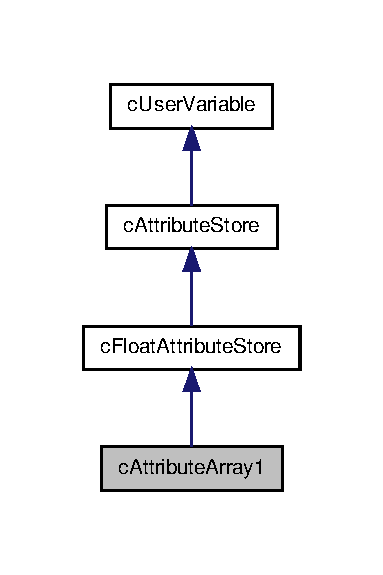
\includegraphics[width=184pt]{classc_attribute_array1__coll__graph}
\end{center}
\end{figure}
\subsection*{Public Member Functions}
\begin{DoxyCompactItemize}
\item 
\hypertarget{classc_attribute_array1_a8020ff4b776221c74f00efc1087344ba}{
void \hyperlink{classc_attribute_array1_a8020ff4b776221c74f00efc1087344ba}{Buffer} ()}
\label{classc_attribute_array1_a8020ff4b776221c74f00efc1087344ba}

\begin{DoxyCompactList}\small\item\em This will Buffer the Data to the graphics card. \end{DoxyCompactList}\end{DoxyCompactItemize}


\subsection{Detailed Description}
This is a specific type of \hyperlink{classc_user_variable}{cUserVariable} for Controlling an array of Attribute with a single value per vertex. See \hyperlink{classc_attribute_store}{cAttributeStore}. 

This Object holds an array of single floats with total number of elements equal to verteces in the object. 
\hypertarget{classc_attribute_array2}{
\section{cAttributeArray2 Class Reference}
\label{classc_attribute_array2}\index{cAttributeArray2@{cAttributeArray2}}
}


This is a specific type of \hyperlink{classc_user_variable}{cUserVariable} for Controlling an array of Attribute with two values per vertex. See \hyperlink{classc_attribute_store}{cAttributeStore}.  




Collaboration diagram for cAttributeArray2:\nopagebreak
\begin{figure}[H]
\begin{center}
\leavevmode
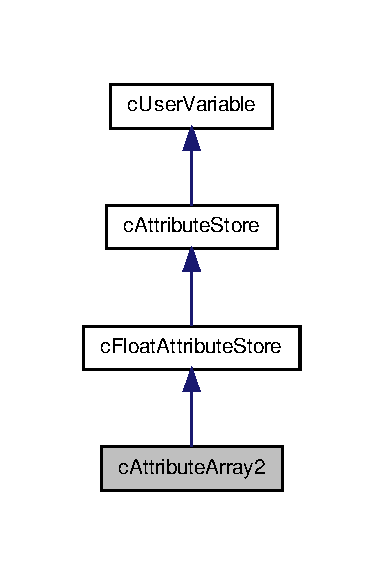
\includegraphics[width=184pt]{classc_attribute_array2__coll__graph}
\end{center}
\end{figure}
\subsection*{Public Member Functions}
\begin{DoxyCompactItemize}
\item 
\hypertarget{classc_attribute_array2_ab668d78ce789f131bb4335ae1f7312df}{
void \hyperlink{classc_attribute_array2_ab668d78ce789f131bb4335ae1f7312df}{Buffer} ()}
\label{classc_attribute_array2_ab668d78ce789f131bb4335ae1f7312df}

\begin{DoxyCompactList}\small\item\em This will Buffer the Data to the graphics card. \end{DoxyCompactList}\end{DoxyCompactItemize}


\subsection{Detailed Description}
This is a specific type of \hyperlink{classc_user_variable}{cUserVariable} for Controlling an array of Attribute with two values per vertex. See \hyperlink{classc_attribute_store}{cAttributeStore}. 

This Object holds an array of two floats with total number of elements equal to twice the verteces in the object. 
\hypertarget{classc_attribute_array3}{
\section{cAttributeArray3 Class Reference}
\label{classc_attribute_array3}\index{cAttributeArray3@{cAttributeArray3}}
}


This is a specific type of \hyperlink{classc_user_variable}{cUserVariable} for Controlling an array of Attribute with three values per vertex. See \hyperlink{classc_attribute_store}{cAttributeStore}.  




Collaboration diagram for cAttributeArray3:\nopagebreak
\begin{figure}[H]
\begin{center}
\leavevmode
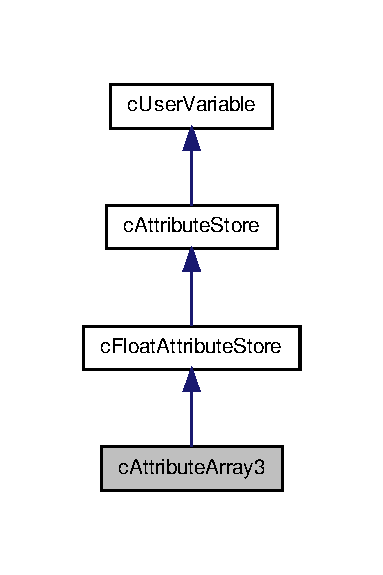
\includegraphics[width=184pt]{classc_attribute_array3__coll__graph}
\end{center}
\end{figure}
\subsection*{Public Member Functions}
\begin{DoxyCompactItemize}
\item 
\hypertarget{classc_attribute_array3_a2c31ff21d2cc86613b8e2fa8da1683e3}{
void \hyperlink{classc_attribute_array3_a2c31ff21d2cc86613b8e2fa8da1683e3}{Buffer} ()}
\label{classc_attribute_array3_a2c31ff21d2cc86613b8e2fa8da1683e3}

\begin{DoxyCompactList}\small\item\em This will Buffer the Data to the graphics card. \end{DoxyCompactList}\end{DoxyCompactItemize}


\subsection{Detailed Description}
This is a specific type of \hyperlink{classc_user_variable}{cUserVariable} for Controlling an array of Attribute with three values per vertex. See \hyperlink{classc_attribute_store}{cAttributeStore}. 

This Object holds an array of three floats with total number of elements equal to three times the verteces in the object. 
\hypertarget{classc_attribute_array4}{
\section{cAttributeArray4 Class Reference}
\label{classc_attribute_array4}\index{cAttributeArray4@{cAttributeArray4}}
}


This is a specific type of \hyperlink{classc_user_variable}{cUserVariable} for Controlling an array of Attribute with four values per vertex. See \hyperlink{classc_attribute_store}{cAttributeStore}.  




Collaboration diagram for cAttributeArray4:\nopagebreak
\begin{figure}[H]
\begin{center}
\leavevmode
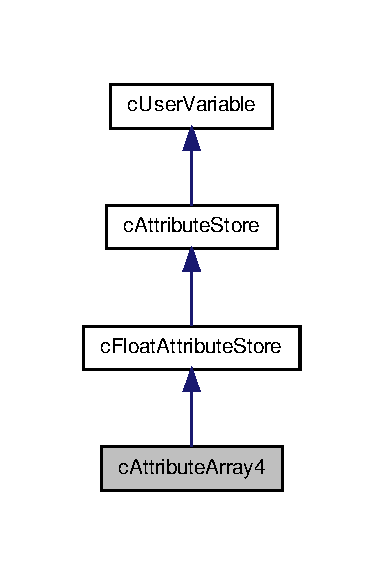
\includegraphics[width=184pt]{classc_attribute_array4__coll__graph}
\end{center}
\end{figure}
\subsection*{Public Member Functions}
\begin{DoxyCompactItemize}
\item 
\hypertarget{classc_attribute_array4_a1ae92d86ffc8e252373d0d316004aafb}{
void \hyperlink{classc_attribute_array4_a1ae92d86ffc8e252373d0d316004aafb}{Buffer} ()}
\label{classc_attribute_array4_a1ae92d86ffc8e252373d0d316004aafb}

\begin{DoxyCompactList}\small\item\em This will Buffer the Data to the graphics card. \end{DoxyCompactList}\end{DoxyCompactItemize}


\subsection{Detailed Description}
This is a specific type of \hyperlink{classc_user_variable}{cUserVariable} for Controlling an array of Attribute with four values per vertex. See \hyperlink{classc_attribute_store}{cAttributeStore}. 

This Object holds an array of four floats with total number of elements equal to four times the verteces in the object. 
\hypertarget{classc_attribute_boolean_array1}{
\section{cAttributeBooleanArray1 Class Reference}
\label{classc_attribute_boolean_array1}\index{cAttributeBooleanArray1@{cAttributeBooleanArray1}}
}


This is a specific type of \hyperlink{classc_user_variable}{cUserVariable} for Controlling an array of Attribute with a single value per vertex. See \hyperlink{classc_attribute_store}{cAttributeStore}.  




Collaboration diagram for cAttributeBooleanArray1:\nopagebreak
\begin{figure}[H]
\begin{center}
\leavevmode
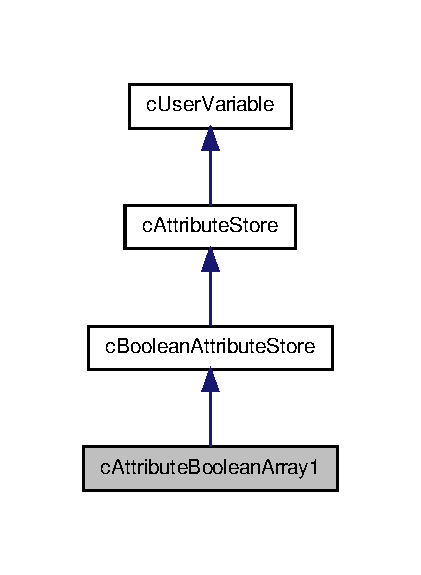
\includegraphics[width=202pt]{classc_attribute_boolean_array1__coll__graph}
\end{center}
\end{figure}
\subsection*{Public Member Functions}
\begin{DoxyCompactItemize}
\item 
\hypertarget{classc_attribute_boolean_array1_aec7dcc6e13a59c1bc4c3b1330d873777}{
void \hyperlink{classc_attribute_boolean_array1_aec7dcc6e13a59c1bc4c3b1330d873777}{Buffer} ()}
\label{classc_attribute_boolean_array1_aec7dcc6e13a59c1bc4c3b1330d873777}

\begin{DoxyCompactList}\small\item\em This will Buffer the Data to the graphics card. \end{DoxyCompactList}\end{DoxyCompactItemize}


\subsection{Detailed Description}
This is a specific type of \hyperlink{classc_user_variable}{cUserVariable} for Controlling an array of Attribute with a single value per vertex. See \hyperlink{classc_attribute_store}{cAttributeStore}. 

This Object holds an array of single booleans with total number of elements equal to verteces in the object. 
\hypertarget{classc_attribute_boolean_array2}{
\section{cAttributeBooleanArray2 Class Reference}
\label{classc_attribute_boolean_array2}\index{cAttributeBooleanArray2@{cAttributeBooleanArray2}}
}


This is a specific type of \hyperlink{classc_user_variable}{cUserVariable} for Controlling an array of Attribute with two values per vertex. See \hyperlink{classc_attribute_store}{cAttributeStore}.  




Collaboration diagram for cAttributeBooleanArray2:\nopagebreak
\begin{figure}[H]
\begin{center}
\leavevmode
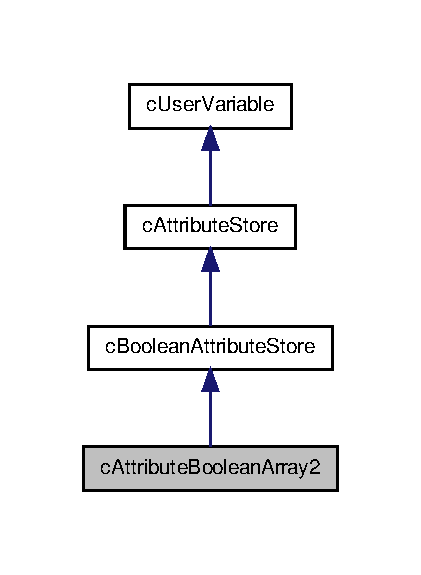
\includegraphics[width=202pt]{classc_attribute_boolean_array2__coll__graph}
\end{center}
\end{figure}
\subsection*{Public Member Functions}
\begin{DoxyCompactItemize}
\item 
\hypertarget{classc_attribute_boolean_array2_a6c979a10c0d436f862211a42908a8acc}{
void \hyperlink{classc_attribute_boolean_array2_a6c979a10c0d436f862211a42908a8acc}{Buffer} ()}
\label{classc_attribute_boolean_array2_a6c979a10c0d436f862211a42908a8acc}

\begin{DoxyCompactList}\small\item\em This will Buffer the Data to the graphics card. \end{DoxyCompactList}\end{DoxyCompactItemize}


\subsection{Detailed Description}
This is a specific type of \hyperlink{classc_user_variable}{cUserVariable} for Controlling an array of Attribute with two values per vertex. See \hyperlink{classc_attribute_store}{cAttributeStore}. 

This Object holds an array of two booleans with total number of elements equal to twice the verteces in the object. 
\hypertarget{classc_attribute_boolean_array3}{
\section{cAttributeBooleanArray3 Class Reference}
\label{classc_attribute_boolean_array3}\index{cAttributeBooleanArray3@{cAttributeBooleanArray3}}
}


This is a specific type of \hyperlink{classc_user_variable}{cUserVariable} for Controlling an array of Attribute with three values per vertex. See \hyperlink{classc_attribute_store}{cAttributeStore}.  




Collaboration diagram for cAttributeBooleanArray3:\nopagebreak
\begin{figure}[H]
\begin{center}
\leavevmode
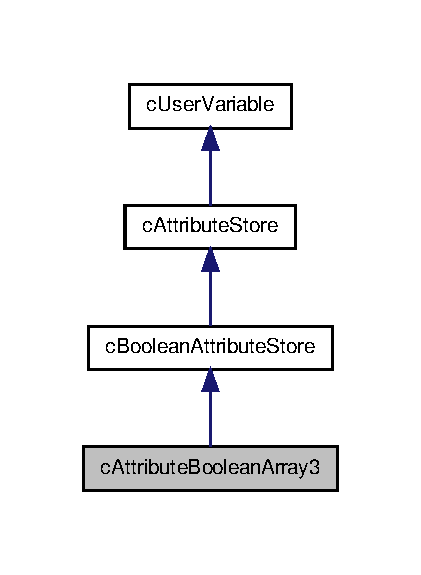
\includegraphics[width=202pt]{classc_attribute_boolean_array3__coll__graph}
\end{center}
\end{figure}
\subsection*{Public Member Functions}
\begin{DoxyCompactItemize}
\item 
\hypertarget{classc_attribute_boolean_array3_a5641b070ad97efab41b2c3aa5337ccab}{
void \hyperlink{classc_attribute_boolean_array3_a5641b070ad97efab41b2c3aa5337ccab}{Buffer} ()}
\label{classc_attribute_boolean_array3_a5641b070ad97efab41b2c3aa5337ccab}

\begin{DoxyCompactList}\small\item\em This will Buffer the Data to the graphics card. \end{DoxyCompactList}\end{DoxyCompactItemize}


\subsection{Detailed Description}
This is a specific type of \hyperlink{classc_user_variable}{cUserVariable} for Controlling an array of Attribute with three values per vertex. See \hyperlink{classc_attribute_store}{cAttributeStore}. 

This Object holds an array of three booleans with total number of elements equal to three times the verteces in the object. 
\hypertarget{classc_attribute_boolean_array4}{
\section{cAttributeBooleanArray4 Class Reference}
\label{classc_attribute_boolean_array4}\index{cAttributeBooleanArray4@{cAttributeBooleanArray4}}
}


This is a specific type of \hyperlink{classc_user_variable}{cUserVariable} for Controlling an array of Attribute with four values per vertex. See \hyperlink{classc_attribute_store}{cAttributeStore}.  




Collaboration diagram for cAttributeBooleanArray4:\nopagebreak
\begin{figure}[H]
\begin{center}
\leavevmode
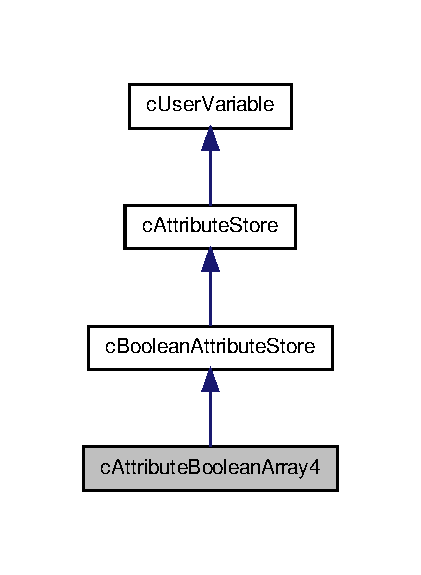
\includegraphics[width=202pt]{classc_attribute_boolean_array4__coll__graph}
\end{center}
\end{figure}
\subsection*{Public Member Functions}
\begin{DoxyCompactItemize}
\item 
\hypertarget{classc_attribute_boolean_array4_a00b56272020a2ca0b4b6e5b8c7b93bf8}{
void \hyperlink{classc_attribute_boolean_array4_a00b56272020a2ca0b4b6e5b8c7b93bf8}{Buffer} ()}
\label{classc_attribute_boolean_array4_a00b56272020a2ca0b4b6e5b8c7b93bf8}

\begin{DoxyCompactList}\small\item\em This will Buffer the Data to the graphics card. \end{DoxyCompactList}\end{DoxyCompactItemize}


\subsection{Detailed Description}
This is a specific type of \hyperlink{classc_user_variable}{cUserVariable} for Controlling an array of Attribute with four values per vertex. See \hyperlink{classc_attribute_store}{cAttributeStore}. 

This Object holds an array of four booleans with total number of elements equal to four times the verteces in the object. 
\hypertarget{classc_attribute_int_array1}{
\section{cAttributeIntArray1 Class Reference}
\label{classc_attribute_int_array1}\index{cAttributeIntArray1@{cAttributeIntArray1}}
}


This is a specific type of \hyperlink{classc_user_variable}{cUserVariable} for Controlling an array of Attribute with a single value per vertex. See \hyperlink{classc_attribute_store}{cAttributeStore}.  




Collaboration diagram for cAttributeIntArray1:\nopagebreak
\begin{figure}[H]
\begin{center}
\leavevmode
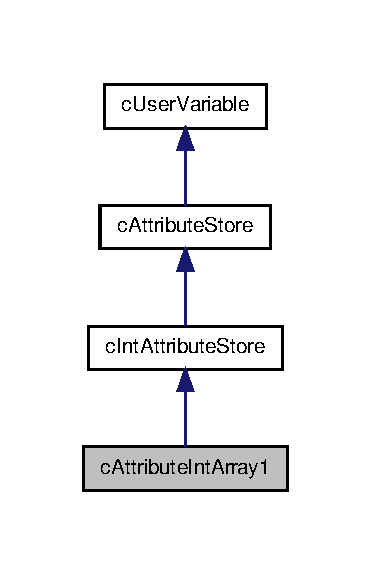
\includegraphics[width=178pt]{classc_attribute_int_array1__coll__graph}
\end{center}
\end{figure}
\subsection*{Public Member Functions}
\begin{DoxyCompactItemize}
\item 
\hypertarget{classc_attribute_int_array1_ab75b77d17c0a0ab5e34fc35d471ace59}{
void \hyperlink{classc_attribute_int_array1_ab75b77d17c0a0ab5e34fc35d471ace59}{Buffer} ()}
\label{classc_attribute_int_array1_ab75b77d17c0a0ab5e34fc35d471ace59}

\begin{DoxyCompactList}\small\item\em This will Buffer the Data to the graphics card. \end{DoxyCompactList}\end{DoxyCompactItemize}


\subsection{Detailed Description}
This is a specific type of \hyperlink{classc_user_variable}{cUserVariable} for Controlling an array of Attribute with a single value per vertex. See \hyperlink{classc_attribute_store}{cAttributeStore}. 

This Object holds an array of single GLint with total number of elements equal to verteces in the object. 
\hypertarget{classc_attribute_int_array2}{
\section{cAttributeIntArray2 Class Reference}
\label{classc_attribute_int_array2}\index{cAttributeIntArray2@{cAttributeIntArray2}}
}


This is a specific type of \hyperlink{classc_user_variable}{cUserVariable} for Controlling an array of Attribute with two values per vertex. See \hyperlink{classc_attribute_store}{cAttributeStore}.  




Collaboration diagram for cAttributeIntArray2:\nopagebreak
\begin{figure}[H]
\begin{center}
\leavevmode
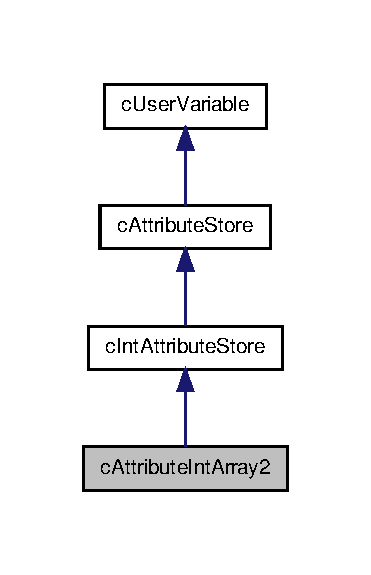
\includegraphics[width=178pt]{classc_attribute_int_array2__coll__graph}
\end{center}
\end{figure}
\subsection*{Public Member Functions}
\begin{DoxyCompactItemize}
\item 
\hypertarget{classc_attribute_int_array2_a7165fa2567c9a78f406b8c2e9d5a82e8}{
void \hyperlink{classc_attribute_int_array2_a7165fa2567c9a78f406b8c2e9d5a82e8}{Buffer} ()}
\label{classc_attribute_int_array2_a7165fa2567c9a78f406b8c2e9d5a82e8}

\begin{DoxyCompactList}\small\item\em This will Buffer the Data to the graphics card. \end{DoxyCompactList}\end{DoxyCompactItemize}


\subsection{Detailed Description}
This is a specific type of \hyperlink{classc_user_variable}{cUserVariable} for Controlling an array of Attribute with two values per vertex. See \hyperlink{classc_attribute_store}{cAttributeStore}. 

This Object holds an array of two GLints with total number of elements equal to twice the verteces in the object. 
\hypertarget{classc_attribute_int_array3}{
\section{cAttributeIntArray3 Class Reference}
\label{classc_attribute_int_array3}\index{cAttributeIntArray3@{cAttributeIntArray3}}
}


This is a specific type of \hyperlink{classc_user_variable}{cUserVariable} for Controlling an array of Attribute with three values per vertex. See \hyperlink{classc_attribute_store}{cAttributeStore}.  




Collaboration diagram for cAttributeIntArray3:\nopagebreak
\begin{figure}[H]
\begin{center}
\leavevmode
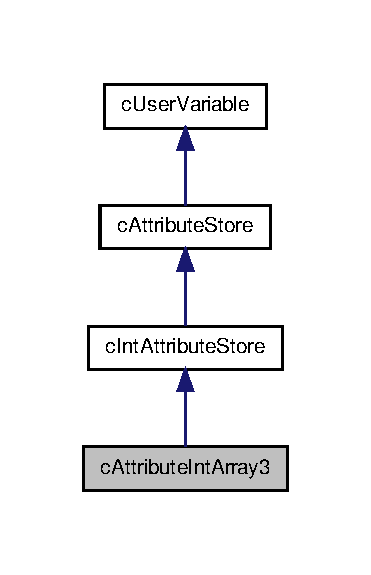
\includegraphics[width=178pt]{classc_attribute_int_array3__coll__graph}
\end{center}
\end{figure}
\subsection*{Public Member Functions}
\begin{DoxyCompactItemize}
\item 
\hypertarget{classc_attribute_int_array3_a53325ec4bacecc7e016061ddab411c23}{
void \hyperlink{classc_attribute_int_array3_a53325ec4bacecc7e016061ddab411c23}{Buffer} ()}
\label{classc_attribute_int_array3_a53325ec4bacecc7e016061ddab411c23}

\begin{DoxyCompactList}\small\item\em This will Buffer the Data to the graphics card. \end{DoxyCompactList}\end{DoxyCompactItemize}


\subsection{Detailed Description}
This is a specific type of \hyperlink{classc_user_variable}{cUserVariable} for Controlling an array of Attribute with three values per vertex. See \hyperlink{classc_attribute_store}{cAttributeStore}. 

This Object holds an array of three GLints with total number of elements equal to three times the verteces in the object. 
\hypertarget{classc_attribute_int_array4}{
\section{cAttributeIntArray4 Class Reference}
\label{classc_attribute_int_array4}\index{cAttributeIntArray4@{cAttributeIntArray4}}
}


This is a specific type of \hyperlink{classc_user_variable}{cUserVariable} for Controlling an array of Attribute with four values per vertex. See \hyperlink{classc_attribute_store}{cAttributeStore}.  




Collaboration diagram for cAttributeIntArray4:\nopagebreak
\begin{figure}[H]
\begin{center}
\leavevmode
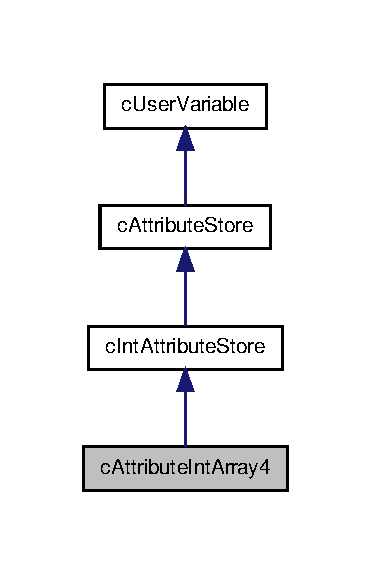
\includegraphics[width=178pt]{classc_attribute_int_array4__coll__graph}
\end{center}
\end{figure}
\subsection*{Public Member Functions}
\begin{DoxyCompactItemize}
\item 
\hypertarget{classc_attribute_int_array4_a5c819b31a4b3966b50b35fe388a1f712}{
void \hyperlink{classc_attribute_int_array4_a5c819b31a4b3966b50b35fe388a1f712}{Buffer} ()}
\label{classc_attribute_int_array4_a5c819b31a4b3966b50b35fe388a1f712}

\begin{DoxyCompactList}\small\item\em This will Buffer the Data to the graphics card. \end{DoxyCompactList}\end{DoxyCompactItemize}


\subsection{Detailed Description}
This is a specific type of \hyperlink{classc_user_variable}{cUserVariable} for Controlling an array of Attribute with four values per vertex. See \hyperlink{classc_attribute_store}{cAttributeStore}. 

This Object holds an array of four GLints with total number of elements equal to four times the verteces in the object. 
\hypertarget{classc_attribute_store}{
\section{cAttributeStore Class Reference}
\label{classc_attribute_store}\index{cAttributeStore@{cAttributeStore}}
}


This is a specific type of \hyperlink{classc_user_variable}{cUserVariable} for Controlling an array of Attribute Values. This is a virtual class type of \hyperlink{classc_user_variable}{cUserVariable}. It is still virtual but is specialised for Attribute variables. This will store a pointer to the array of data. This means the user can hand the array to the class and update it, resulting in update every frame. The user must not delete the array or the system will end up reading random data. Attribute Variables are variables which are set for every vertex in the object.  




Collaboration diagram for cAttributeStore:\nopagebreak
\begin{figure}[H]
\begin{center}
\leavevmode
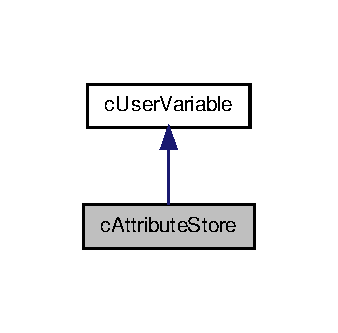
\includegraphics[width=162pt]{classc_attribute_store__coll__graph}
\end{center}
\end{figure}
\subsection*{Public Member Functions}
\begin{DoxyCompactItemize}
\item 
\hypertarget{classc_attribute_store_a459866aef786182597d456dc79e26e58}{
void \hyperlink{classc_attribute_store_a459866aef786182597d456dc79e26e58}{Write} ()}
\label{classc_attribute_store_a459866aef786182597d456dc79e26e58}

\begin{DoxyCompactList}\small\item\em Function to write the buffered value to the graphics card. \end{DoxyCompactList}\item 
\hypertarget{classc_attribute_store_a69cb1bcc9f595cd720314c244d6d793a}{
void \hyperlink{classc_attribute_store_a69cb1bcc9f595cd720314c244d6d793a}{DataValue} (void $\ast$lpData, uint32 liElements)=0}
\label{classc_attribute_store_a69cb1bcc9f595cd720314c244d6d793a}

\begin{DoxyCompactList}\small\item\em This will Set the Array of Data an Attribute Variable will Use. This will copy the data. It will not automatically update, but the data can be deallocated at any time. \end{DoxyCompactList}\item 
\hypertarget{classc_attribute_store_a7acc5153925532b260f26b90fcfeeb32}{
void \hyperlink{classc_attribute_store_a7acc5153925532b260f26b90fcfeeb32}{DataValue} (void $\ast$lpData)}
\label{classc_attribute_store_a7acc5153925532b260f26b90fcfeeb32}

\begin{DoxyCompactList}\small\item\em This will Set the Data a Uniform Variable will Use. This will copy the data. It will not automatically update, but the data can be deallocated at any time. \end{DoxyCompactList}\item 
\hypertarget{classc_attribute_store_a07f2f617cc6fb0bad9ba6337e0b0991e}{
void \hyperlink{classc_attribute_store_a07f2f617cc6fb0bad9ba6337e0b0991e}{DataPointer} (void $\ast$lpData)}
\label{classc_attribute_store_a07f2f617cc6fb0bad9ba6337e0b0991e}

\begin{DoxyCompactList}\small\item\em This will Set the Data a Uniform Variable will Use. This will not copy the data, but will store a pointer to the data. It will automatically update, but the data passed to it should not be deallocated while the shader is in use. \end{DoxyCompactList}\item 
\hypertarget{classc_attribute_store_a2cafff0276874cf2b4be95ae2ed194fe}{
void \hyperlink{classc_attribute_store_a2cafff0276874cf2b4be95ae2ed194fe}{DataPointer} (void $\ast$lpData, uint32 liElements)=0}
\label{classc_attribute_store_a2cafff0276874cf2b4be95ae2ed194fe}

\begin{DoxyCompactList}\small\item\em This will Set the Array of Data an Attribute Variable will Use. This will not copy the data, but will store a pointer to the data. It will automatically update, but the data passed to it should not be deallocated while the shader is in use. \end{DoxyCompactList}\end{DoxyCompactItemize}


\subsection{Detailed Description}
This is a specific type of \hyperlink{classc_user_variable}{cUserVariable} for Controlling an array of Attribute Values. This is a virtual class type of \hyperlink{classc_user_variable}{cUserVariable}. It is still virtual but is specialised for Attribute variables. This will store a pointer to the array of data. This means the user can hand the array to the class and update it, resulting in update every frame. The user must not delete the array or the system will end up reading random data. Attribute Variables are variables which are set for every vertex in the object. 
\hypertarget{classc_audio_buffer}{
\section{cAudioBuffer Class Reference}
\label{classc_audio_buffer}\index{cAudioBuffer@{cAudioBuffer}}
}


This class will create a buffer space to store sound data. This class will create and initialise an OpenAL buffer. The Buffer stores the sound data and is linked to a \hyperlink{classc_audio_object}{cAudioObject} to allow it to be played.  


\subsection*{Public Member Functions}
\begin{DoxyCompactItemize}
\item 
\hypertarget{classc_audio_buffer_adae216a1c736e8474f8db45319f97467}{
\hyperlink{classc_audio_buffer_adae216a1c736e8474f8db45319f97467}{cAudioBuffer} ()}
\label{classc_audio_buffer_adae216a1c736e8474f8db45319f97467}

\begin{DoxyCompactList}\small\item\em Constructor to Initialise a Buffer. \end{DoxyCompactList}\item 
\hypertarget{classc_audio_buffer_a4fb260df2f23cf5c8ec4b557555df89b}{
ALuint \hyperlink{classc_audio_buffer_a4fb260df2f23cf5c8ec4b557555df89b}{Buffer} ()}
\label{classc_audio_buffer_a4fb260df2f23cf5c8ec4b557555df89b}

\begin{DoxyCompactList}\small\item\em This will return the ID of the buffer owned by this class. \end{DoxyCompactList}\end{DoxyCompactItemize}


\subsection{Detailed Description}
This class will create a buffer space to store sound data. This class will create and initialise an OpenAL buffer. The Buffer stores the sound data and is linked to a \hyperlink{classc_audio_object}{cAudioObject} to allow it to be played. 
\hypertarget{classc_audio_device}{
\section{cAudioDevice Class Reference}
\label{classc_audio_device}\index{cAudioDevice@{cAudioDevice}}
}


This class will initialise the sound card. This class will initialise an audio device so sounds can be played on the system.  




Collaboration diagram for cAudioDevice:\nopagebreak
\begin{figure}[H]
\begin{center}
\leavevmode
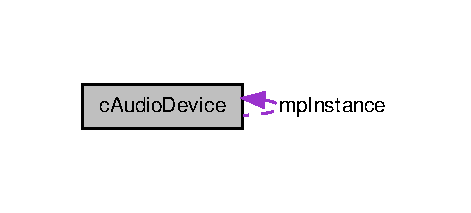
\includegraphics[width=226pt]{classc_audio_device__coll__graph}
\end{center}
\end{figure}
\subsection*{Public Member Functions}
\begin{DoxyCompactItemize}
\item 
\hypertarget{classc_audio_device_a66ac901442496247a1e9a9ea7ef44120}{
\hyperlink{classc_audio_device_a66ac901442496247a1e9a9ea7ef44120}{cAudioDevice} ()}
\label{classc_audio_device_a66ac901442496247a1e9a9ea7ef44120}

\begin{DoxyCompactList}\small\item\em Constructor will start and initialise an OpenAL system. \end{DoxyCompactList}\end{DoxyCompactItemize}
\subsection*{Static Public Member Functions}
\begin{DoxyCompactItemize}
\item 
\hypertarget{classc_audio_device_aebae28f8c27622a408e616c50e096e85}{
static \hyperlink{classc_audio_device}{cAudioDevice} $\ast$ \hyperlink{classc_audio_device_aebae28f8c27622a408e616c50e096e85}{Instance} ()}
\label{classc_audio_device_aebae28f8c27622a408e616c50e096e85}

\begin{DoxyCompactList}\small\item\em This Function will return a pointer to the current OpenAL Audio Device. \end{DoxyCompactList}\end{DoxyCompactItemize}


\subsection{Detailed Description}
This class will initialise the sound card. This class will initialise an audio device so sounds can be played on the system. 
\hypertarget{classc_audio_listener}{
\section{cAudioListener Class Reference}
\label{classc_audio_listener}\index{cAudioListener@{cAudioListener}}
}


This controls the state of the Listener. This is the assumed position, facing and velocity of the user for the purposes of Sound.  




Collaboration diagram for cAudioListener:\nopagebreak
\begin{figure}[H]
\begin{center}
\leavevmode
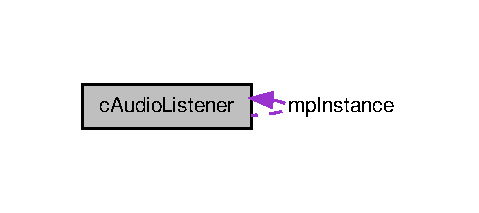
\includegraphics[width=230pt]{classc_audio_listener__coll__graph}
\end{center}
\end{figure}
\subsection*{Static Public Member Functions}
\begin{DoxyCompactItemize}
\item 
\hypertarget{classc_audio_listener_a2269493a4603684e6effdf9427fee175}{
static \hyperlink{classc_audio_listener}{cAudioListener} $\ast$ \hyperlink{classc_audio_listener_a2269493a4603684e6effdf9427fee175}{Instance} ()}
\label{classc_audio_listener_a2269493a4603684e6effdf9427fee175}

\begin{DoxyCompactList}\small\item\em Gets a pointer to the \hyperlink{classc_audio_listener}{cAudioListener} singleton. \end{DoxyCompactList}\end{DoxyCompactItemize}
\subsection*{Friends}
\begin{DoxyCompactItemize}
\item 
\hypertarget{classc_audio_listener_a62507a4ca159e2ef51ac9bc1bc5bfeb6}{
class \hyperlink{classc_audio_listener_a62507a4ca159e2ef51ac9bc1bc5bfeb6}{cAudioObject}}
\label{classc_audio_listener_a62507a4ca159e2ef51ac9bc1bc5bfeb6}

\end{DoxyCompactItemize}


\subsection{Detailed Description}
This controls the state of the Listener. This is the assumed position, facing and velocity of the user for the purposes of Sound. 
\hypertarget{classc_audio_object}{
\section{cAudioObject Class Reference}
\label{classc_audio_object}\index{cAudioObject@{cAudioObject}}
}


This class will allow a sound to be played. This class will link an audio source and a buffer, This allows the sound data stored in the buffer to be played through the source. Each source is an audio channel and can only play one sound at a time.  




Collaboration diagram for cAudioObject:
\nopagebreak
\begin{figure}[H]
\begin{center}
\leavevmode
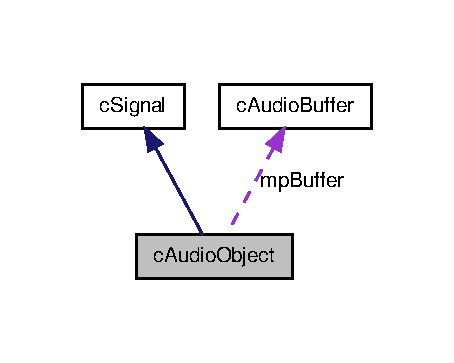
\includegraphics[width=157pt]{classc_audio_object__coll__graph}
\end{center}
\end{figure}
\subsection*{Public Member Functions}
\begin{DoxyCompactItemize}
\item 
\hyperlink{classc_audio_object_a1a44ae87c2bf5e43aff66624a42771fe}{cAudioObject} ()
\begin{DoxyCompactList}\small\item\em This will create an OpenAL source for this object, without linking any cAudioBuffers to it. \item\end{DoxyCompactList}\item 
\hyperlink{classc_audio_object_a172d5d9e89376a0c505fa051e9d02919}{cAudioObject} (\hyperlink{classc_audio_buffer}{cAudioBuffer} $\ast$lpBuffer)
\begin{DoxyCompactList}\small\item\em This will create an OpenAL source and link this object to a buffer. \item\end{DoxyCompactList}\item 
\hyperlink{classc_audio_object_a57baf1e1384c3307ce8db629c9b2a59f}{$\sim$cAudioObject} ()
\item 
void \hyperlink{classc_audio_object_aaa2c81875452c51ecd3979a0b1b2c8b1}{SetBuffer} (\hyperlink{classc_audio_buffer}{cAudioBuffer} $\ast$lpBuffer)
\begin{DoxyCompactList}\small\item\em This will link the OpenAL buffer pointed to by lpBuffer to this Audio Object ready to be played. \item\end{DoxyCompactList}\item 
void \hyperlink{classc_audio_object_a2e7c8dc824eef10006f0f1c2824f10cd}{Play} ()
\begin{DoxyCompactList}\small\item\em This will play a sound through the OpenAL source from the buffer. \item\end{DoxyCompactList}\item 
ALuint \hyperlink{classc_audio_object_adb134027851226f2f5a446a3d885f26e}{Source} ()
\begin{DoxyCompactList}\small\item\em This will return the ID of the OpenAL ID. \item\end{DoxyCompactList}\end{DoxyCompactItemize}


\subsection{Detailed Description}
This class will allow a sound to be played. This class will link an audio source and a buffer, This allows the sound data stored in the buffer to be played through the source. Each source is an audio channel and can only play one sound at a time. 

Definition at line 7 of file WTcAudioObject.h.



\subsection{Constructor \& Destructor Documentation}
\hypertarget{classc_audio_object_a1a44ae87c2bf5e43aff66624a42771fe}{
\index{cAudioObject@{cAudioObject}!cAudioObject@{cAudioObject}}
\index{cAudioObject@{cAudioObject}!cAudioObject@{cAudioObject}}
\subsubsection[{cAudioObject}]{\setlength{\rightskip}{0pt plus 5cm}cAudioObject::cAudioObject (
\begin{DoxyParamCaption}
{}
\end{DoxyParamCaption}
)}}
\label{classc_audio_object_a1a44ae87c2bf5e43aff66624a42771fe}


This will create an OpenAL source for this object, without linking any cAudioBuffers to it. 



Definition at line 3 of file WTcAudioObject.cpp.

\hypertarget{classc_audio_object_a172d5d9e89376a0c505fa051e9d02919}{
\index{cAudioObject@{cAudioObject}!cAudioObject@{cAudioObject}}
\index{cAudioObject@{cAudioObject}!cAudioObject@{cAudioObject}}
\subsubsection[{cAudioObject}]{\setlength{\rightskip}{0pt plus 5cm}cAudioObject::cAudioObject (
\begin{DoxyParamCaption}
\item[{{\bf cAudioBuffer} $\ast$}]{lpBuffer}
\end{DoxyParamCaption}
)}}
\label{classc_audio_object_a172d5d9e89376a0c505fa051e9d02919}


This will create an OpenAL source and link this object to a buffer. 



Definition at line 9 of file WTcAudioObject.cpp.

\hypertarget{classc_audio_object_a57baf1e1384c3307ce8db629c9b2a59f}{
\index{cAudioObject@{cAudioObject}!$\sim$cAudioObject@{$\sim$cAudioObject}}
\index{$\sim$cAudioObject@{$\sim$cAudioObject}!cAudioObject@{cAudioObject}}
\subsubsection[{$\sim$cAudioObject}]{\setlength{\rightskip}{0pt plus 5cm}cAudioObject::$\sim$cAudioObject (
\begin{DoxyParamCaption}
{}
\end{DoxyParamCaption}
)}}
\label{classc_audio_object_a57baf1e1384c3307ce8db629c9b2a59f}


Definition at line 17 of file WTcAudioObject.cpp.



\subsection{Member Function Documentation}
\hypertarget{classc_audio_object_a2e7c8dc824eef10006f0f1c2824f10cd}{
\index{cAudioObject@{cAudioObject}!Play@{Play}}
\index{Play@{Play}!cAudioObject@{cAudioObject}}
\subsubsection[{Play}]{\setlength{\rightskip}{0pt plus 5cm}void cAudioObject::Play (
\begin{DoxyParamCaption}
{}
\end{DoxyParamCaption}
)}}
\label{classc_audio_object_a2e7c8dc824eef10006f0f1c2824f10cd}


This will play a sound through the OpenAL source from the buffer. 



Definition at line 22 of file WTcAudioObject.cpp.

\hypertarget{classc_audio_object_aaa2c81875452c51ecd3979a0b1b2c8b1}{
\index{cAudioObject@{cAudioObject}!SetBuffer@{SetBuffer}}
\index{SetBuffer@{SetBuffer}!cAudioObject@{cAudioObject}}
\subsubsection[{SetBuffer}]{\setlength{\rightskip}{0pt plus 5cm}void cAudioObject::SetBuffer (
\begin{DoxyParamCaption}
\item[{{\bf cAudioBuffer} $\ast$}]{lpBuffer}
\end{DoxyParamCaption}
)}}
\label{classc_audio_object_aaa2c81875452c51ecd3979a0b1b2c8b1}


This will link the OpenAL buffer pointed to by lpBuffer to this Audio Object ready to be played. 



Definition at line 27 of file WTcAudioObject.cpp.

\hypertarget{classc_audio_object_adb134027851226f2f5a446a3d885f26e}{
\index{cAudioObject@{cAudioObject}!Source@{Source}}
\index{Source@{Source}!cAudioObject@{cAudioObject}}
\subsubsection[{Source}]{\setlength{\rightskip}{0pt plus 5cm}ALuint cAudioObject::Source (
\begin{DoxyParamCaption}
{}
\end{DoxyParamCaption}
)}}
\label{classc_audio_object_adb134027851226f2f5a446a3d885f26e}


This will return the ID of the OpenAL ID. 



Definition at line 35 of file WTcAudioObject.cpp.


\hypertarget{classc_beam_collision}{
\section{cBeamCollision Class Reference}
\label{classc_beam_collision}\index{cBeamCollision@{cBeamCollision}}
}


Collaboration diagram for cBeamCollision:\nopagebreak
\begin{figure}[H]
\begin{center}
\leavevmode
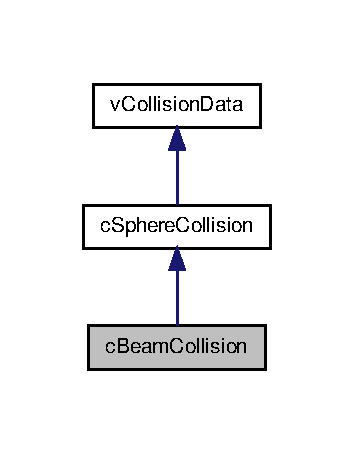
\includegraphics[width=170pt]{classc_beam_collision__coll__graph}
\end{center}
\end{figure}
\subsection*{Public Member Functions}
\begin{DoxyCompactItemize}
\item 
\hypertarget{classc_beam_collision_a8341836a9d69ea56fa119276b6ed29f4}{
void \hyperlink{classc_beam_collision_a8341836a9d69ea56fa119276b6ed29f4}{BuildObject} (float lfLength, float lfRadius)}
\label{classc_beam_collision_a8341836a9d69ea56fa119276b6ed29f4}

\begin{DoxyCompactList}\small\item\em This will generate a \hyperlink{classc_beam_collision}{cBeamCollision} data set of length lfength and Radius lfRadius. \end{DoxyCompactList}\item 
\hypertarget{classc_beam_collision_ae2cb900aab3fc1562c1162e6b5ab98f5}{
virtual \hyperlink{classc_beam_collision}{cBeamCollision} $\ast$ \hyperlink{classc_beam_collision_ae2cb900aab3fc1562c1162e6b5ab98f5}{Beam} ()}
\label{classc_beam_collision_ae2cb900aab3fc1562c1162e6b5ab98f5}

\begin{DoxyCompactList}\small\item\em Will return a pointer if this object contains a Beam collision data object. Otherwise returns 0;. \end{DoxyCompactList}\item 
\hypertarget{classc_beam_collision_a26f8662d41bc325dd14e3be9e7f1d1e9}{
virtual \hyperlink{classc_ray_collision}{cRayCollision} $\ast$ \hyperlink{classc_beam_collision_a26f8662d41bc325dd14e3be9e7f1d1e9}{Ray} ()}
\label{classc_beam_collision_a26f8662d41bc325dd14e3be9e7f1d1e9}

\begin{DoxyCompactList}\small\item\em Will return a pointer if this object contains a Ray collision data object. Otherwise returns 0;. \end{DoxyCompactList}\item 
\hypertarget{classc_beam_collision_a9c4fdda013d88c516edbb470ce9fab01}{
float $\ast$ \hyperlink{classc_beam_collision_a9c4fdda013d88c516edbb470ce9fab01}{RayVector} ()}
\label{classc_beam_collision_a9c4fdda013d88c516edbb470ce9fab01}

\begin{DoxyCompactList}\small\item\em Will return a float array with the beams global vector representing the direction it is pointing in. This should be normalised. \end{DoxyCompactList}\item 
\hypertarget{classc_beam_collision_a2eb26dfd4255ce8a2a10a7b142fb7f42}{
float \hyperlink{classc_beam_collision_a2eb26dfd4255ce8a2a10a7b142fb7f42}{Length} ()}
\label{classc_beam_collision_a2eb26dfd4255ce8a2a10a7b142fb7f42}

\begin{DoxyCompactList}\small\item\em Will return the length of the beam. \end{DoxyCompactList}\item 
\hypertarget{classc_beam_collision_ab7a645cc905fc9c62bfd6a1440d349b1}{
uint8 \hyperlink{classc_beam_collision_ab7a645cc905fc9c62bfd6a1440d349b1}{Type} ()}
\label{classc_beam_collision_ab7a645cc905fc9c62bfd6a1440d349b1}

\begin{DoxyCompactList}\small\item\em Will return the Objects Type. \end{DoxyCompactList}\end{DoxyCompactItemize}
\subsection*{Friends}
\begin{DoxyCompactItemize}
\item 
\hypertarget{classc_beam_collision_a70bfdc2c4682463db2e7755ec3e6440e}{
class \hyperlink{classc_beam_collision_a70bfdc2c4682463db2e7755ec3e6440e}{cMouse}}
\label{classc_beam_collision_a70bfdc2c4682463db2e7755ec3e6440e}

\end{DoxyCompactItemize}


\subsection{Detailed Description}
This class is for representing beams. Think energy beams. The system will assume that the object is a sphere of radius equal to the value set in SetSize(float $\ast$lfSize). The system will project the beam from the centrepoint of the beams current position in the direction of the Z-\/axis for a distance of mfLength. This is a fast and perfect (if the beam is a cylinder capped with hemi-\/spheres) way of colliding straight energy beams. See \hyperlink{classv_collision_data}{vCollisionData} for more information. 
\hypertarget{classc_beam_mesh}{
\section{cBeamMesh Class Reference}
\label{classc_beam_mesh}\index{cBeamMesh@{cBeamMesh}}
}


A Procedurally generated cylindrical Renderable Object. This class will generate a cylinder with specified dimensions and segments. The origin for the cylinder is in the radial center of one end of the cylinder.  




Collaboration diagram for cBeamMesh:\nopagebreak
\begin{figure}[H]
\begin{center}
\leavevmode
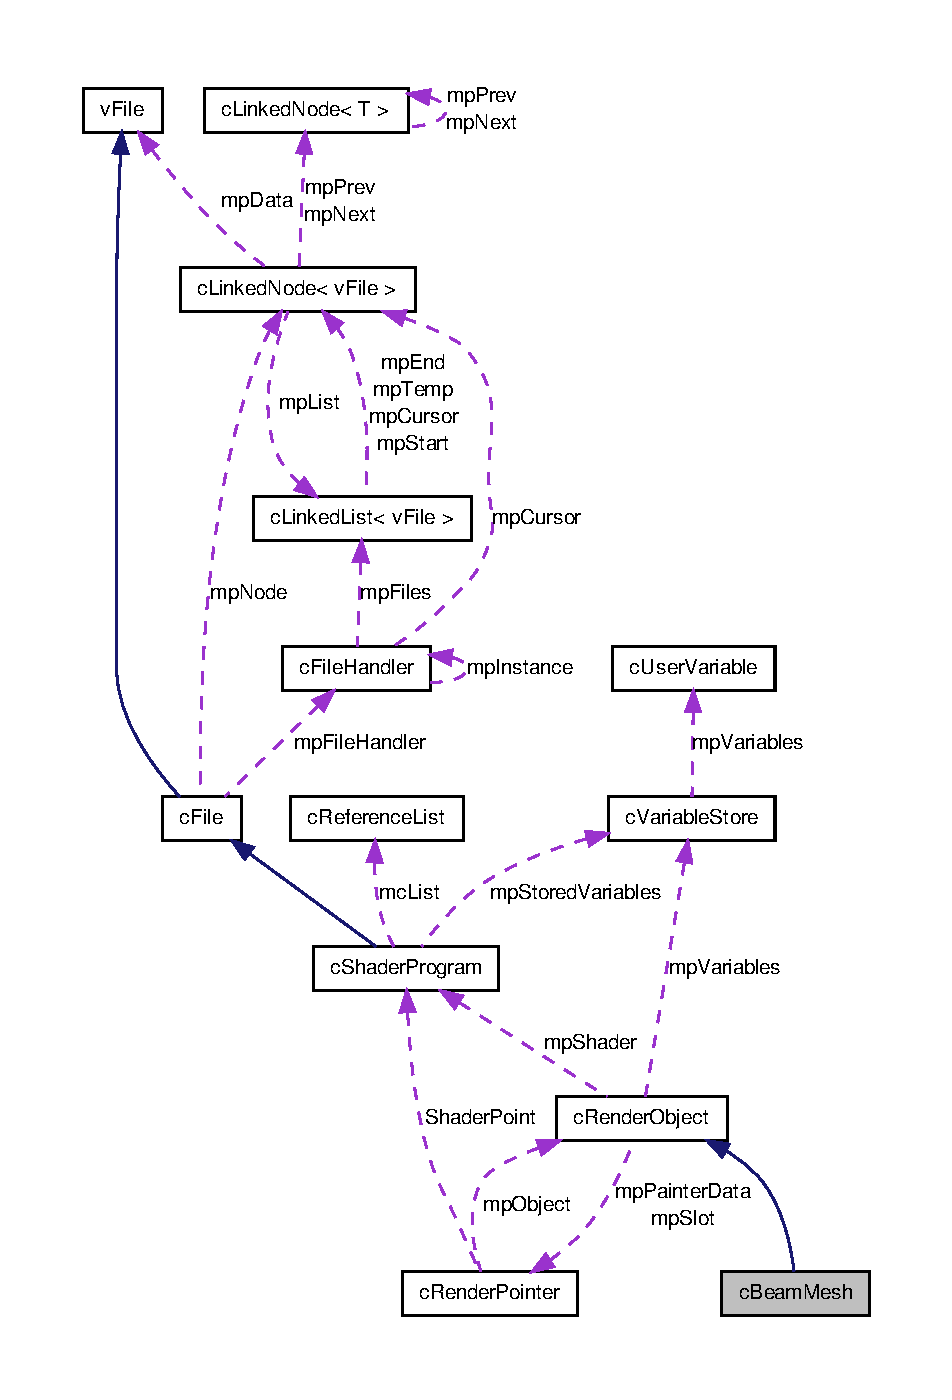
\includegraphics[width=400pt]{classc_beam_mesh__coll__graph}
\end{center}
\end{figure}
\subsection*{Public Member Functions}
\begin{DoxyCompactItemize}
\item 
\hypertarget{classc_beam_mesh_acf82cda9d282def977903ff877f36a26}{
\hyperlink{classc_beam_mesh_acf82cda9d282def977903ff877f36a26}{cBeamMesh} (float Radius=0.1f, float Length=1.0f, uint16 Segments=6, vRenderNode $\ast$lpNode=cCamera::Instance()-\/$>$RenderList())}
\label{classc_beam_mesh_acf82cda9d282def977903ff877f36a26}

\begin{DoxyCompactList}\small\item\em Constructor to Create a Beam with the specified Dimensions. Segments must be an even integer. \end{DoxyCompactList}\item 
\hypertarget{classc_beam_mesh_a1d2f2bfef0e3f96597ae6e1e73072030}{
void \hyperlink{classc_beam_mesh_a1d2f2bfef0e3f96597ae6e1e73072030}{Length} (float Length)}
\label{classc_beam_mesh_a1d2f2bfef0e3f96597ae6e1e73072030}

\begin{DoxyCompactList}\small\item\em Sets the Length of the Cylinder. \end{DoxyCompactList}\item 
\hypertarget{classc_beam_mesh_ac11934e813765321e76405cd96304088}{
void \hyperlink{classc_beam_mesh_ac11934e813765321e76405cd96304088}{Radius} (float Radius)}
\label{classc_beam_mesh_ac11934e813765321e76405cd96304088}

\begin{DoxyCompactList}\small\item\em Sets the Radius of the Cylinder. \end{DoxyCompactList}\item 
\hypertarget{classc_beam_mesh_ab59d3bb8c0a5c2944a206deaca3d2022}{
void \hyperlink{classc_beam_mesh_ab59d3bb8c0a5c2944a206deaca3d2022}{GenerateData} (float Radius, float Length, uint16 Segments)}
\label{classc_beam_mesh_ab59d3bb8c0a5c2944a206deaca3d2022}

\begin{DoxyCompactList}\small\item\em Will regenerate the cylinder with the specified Specifications. \end{DoxyCompactList}\item 
\hypertarget{classc_beam_mesh_aa4daa383162c2560c1c5ed47d22484e5}{
float \hyperlink{classc_beam_mesh_aa4daa383162c2560c1c5ed47d22484e5}{Length} ()}
\label{classc_beam_mesh_aa4daa383162c2560c1c5ed47d22484e5}

\begin{DoxyCompactList}\small\item\em Returns the current Length of the Cylinder. \end{DoxyCompactList}\item 
\hypertarget{classc_beam_mesh_a6068db701b4835449bd40a437e3ee908}{
float \hyperlink{classc_beam_mesh_a6068db701b4835449bd40a437e3ee908}{Radius} ()}
\label{classc_beam_mesh_a6068db701b4835449bd40a437e3ee908}

\begin{DoxyCompactList}\small\item\em Returns the current Radius of the Cylinder. \end{DoxyCompactList}\end{DoxyCompactItemize}


\subsection{Detailed Description}
A Procedurally generated cylindrical Renderable Object. This class will generate a cylinder with specified dimensions and segments. The origin for the cylinder is in the radial center of one end of the cylinder. 
\hypertarget{classc_boolean_attribute_store}{
\section{cBooleanAttributeStore Class Reference}
\label{classc_boolean_attribute_store}\index{cBooleanAttributeStore@{cBooleanAttributeStore}}
}


More Specific Base class for Attribute Handling classes. Suitable for bool Variables. see \hyperlink{classc_attribute_boolean_array1}{cAttributeBooleanArray1}, \hyperlink{classc_attribute_boolean_array2}{cAttributeBooleanArray2}, \hyperlink{classc_attribute_boolean_array3}{cAttributeBooleanArray3}, \hyperlink{classc_attribute_boolean_array4}{cAttributeBooleanArray4}.  




Collaboration diagram for cBooleanAttributeStore:\nopagebreak
\begin{figure}[H]
\begin{center}
\leavevmode
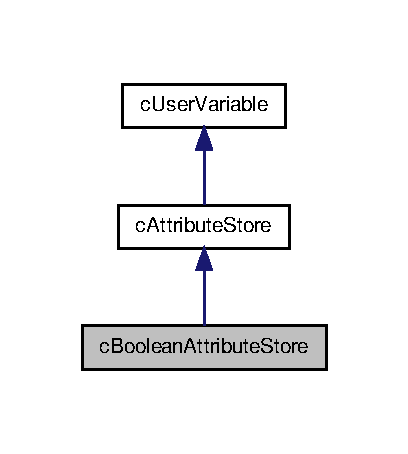
\includegraphics[width=196pt]{classc_boolean_attribute_store__coll__graph}
\end{center}
\end{figure}
\subsection*{Public Member Functions}
\begin{DoxyCompactItemize}
\item 
\hypertarget{classc_boolean_attribute_store_af1ea16395c02827582c8aac43a713fa1}{
void \hyperlink{classc_boolean_attribute_store_af1ea16395c02827582c8aac43a713fa1}{DataValue} (void $\ast$lpData, uint32 liElements)}
\label{classc_boolean_attribute_store_af1ea16395c02827582c8aac43a713fa1}

\begin{DoxyCompactList}\small\item\em This will Set the Array of Data an Attribute Variable will Use. This will copy the data. It will not automatically update, but the data can be deallocated at any time. \end{DoxyCompactList}\item 
\hypertarget{classc_boolean_attribute_store_a17ae26d7f4a3d7edfeb9748d20296e13}{
void \hyperlink{classc_boolean_attribute_store_a17ae26d7f4a3d7edfeb9748d20296e13}{DataPointer} (void $\ast$lpData, uint32 liElements)}
\label{classc_boolean_attribute_store_a17ae26d7f4a3d7edfeb9748d20296e13}

\begin{DoxyCompactList}\small\item\em This will Set the Array of Data an Attribute Variable will Use. This will not copy the data, but will store a pointer to the data. It will automatically update, but the data passed to it should not be deallocated while the shader is in use. \end{DoxyCompactList}\item 
\hypertarget{classc_boolean_attribute_store_a5acc1279e3327f694a39f486b33f41c8}{
void $\ast$ \hyperlink{classc_boolean_attribute_store_a5acc1279e3327f694a39f486b33f41c8}{Data} ()}
\label{classc_boolean_attribute_store_a5acc1279e3327f694a39f486b33f41c8}

\begin{DoxyCompactList}\small\item\em This will return the data the Function is pointing at. \end{DoxyCompactList}\end{DoxyCompactItemize}


\subsection{Detailed Description}
More Specific Base class for Attribute Handling classes. Suitable for bool Variables. see \hyperlink{classc_attribute_boolean_array1}{cAttributeBooleanArray1}, \hyperlink{classc_attribute_boolean_array2}{cAttributeBooleanArray2}, \hyperlink{classc_attribute_boolean_array3}{cAttributeBooleanArray3}, \hyperlink{classc_attribute_boolean_array4}{cAttributeBooleanArray4}. 
\hypertarget{classc_boolean_uniform_store}{
\section{cBooleanUniformStore Class Reference}
\label{classc_boolean_uniform_store}\index{cBooleanUniformStore@{cBooleanUniformStore}}
}


More Specific Base class for Uniform Handling classes. Suitable for Boolean Variables see \hyperlink{classc_uniform_boolean_vector1}{cUniformBooleanVector1}, \hyperlink{classc_uniform_boolean_vector2}{cUniformBooleanVector2}, \hyperlink{classc_uniform_boolean_vector3}{cUniformBooleanVector3}, \hyperlink{classc_uniform_boolean_vector4}{cUniformBooleanVector4}.  




Collaboration diagram for cBooleanUniformStore:\nopagebreak
\begin{figure}[H]
\begin{center}
\leavevmode
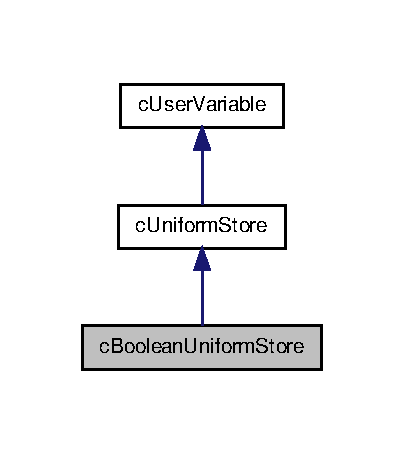
\includegraphics[width=194pt]{classc_boolean_uniform_store__coll__graph}
\end{center}
\end{figure}
\subsection*{Public Member Functions}
\begin{DoxyCompactItemize}
\item 
\hypertarget{classc_boolean_uniform_store_af080d19e87d31b65879ed4e2facd2330}{
void \hyperlink{classc_boolean_uniform_store_af080d19e87d31b65879ed4e2facd2330}{DataPointer} (void $\ast$lpData)}
\label{classc_boolean_uniform_store_af080d19e87d31b65879ed4e2facd2330}

\begin{DoxyCompactList}\small\item\em This will Set the Data a Uniform Variable will Use. This will not copy the data, but will store a pointer to the data. It will automatically update, but the data passed to it should not be deallocated while the shader is in use. \end{DoxyCompactList}\end{DoxyCompactItemize}


\subsection{Detailed Description}
More Specific Base class for Uniform Handling classes. Suitable for Boolean Variables see \hyperlink{classc_uniform_boolean_vector1}{cUniformBooleanVector1}, \hyperlink{classc_uniform_boolean_vector2}{cUniformBooleanVector2}, \hyperlink{classc_uniform_boolean_vector3}{cUniformBooleanVector3}, \hyperlink{classc_uniform_boolean_vector4}{cUniformBooleanVector4}. 
\hypertarget{classc_button}{
\section{cButton Class Reference}
\label{classc_button}\index{cButton@{cButton}}
}


Renderable Button object for displaying an object as a rendered image. Takes an image and will render it as a 2D image. Will check for mouse collisions and mouse button clicks to determine how user has interacted with the button. see \hyperlink{classc_button_base}{cButtonBase} for Mouse Interaction Functions.  




Collaboration diagram for cButton:\nopagebreak
\begin{figure}[H]
\begin{center}
\leavevmode
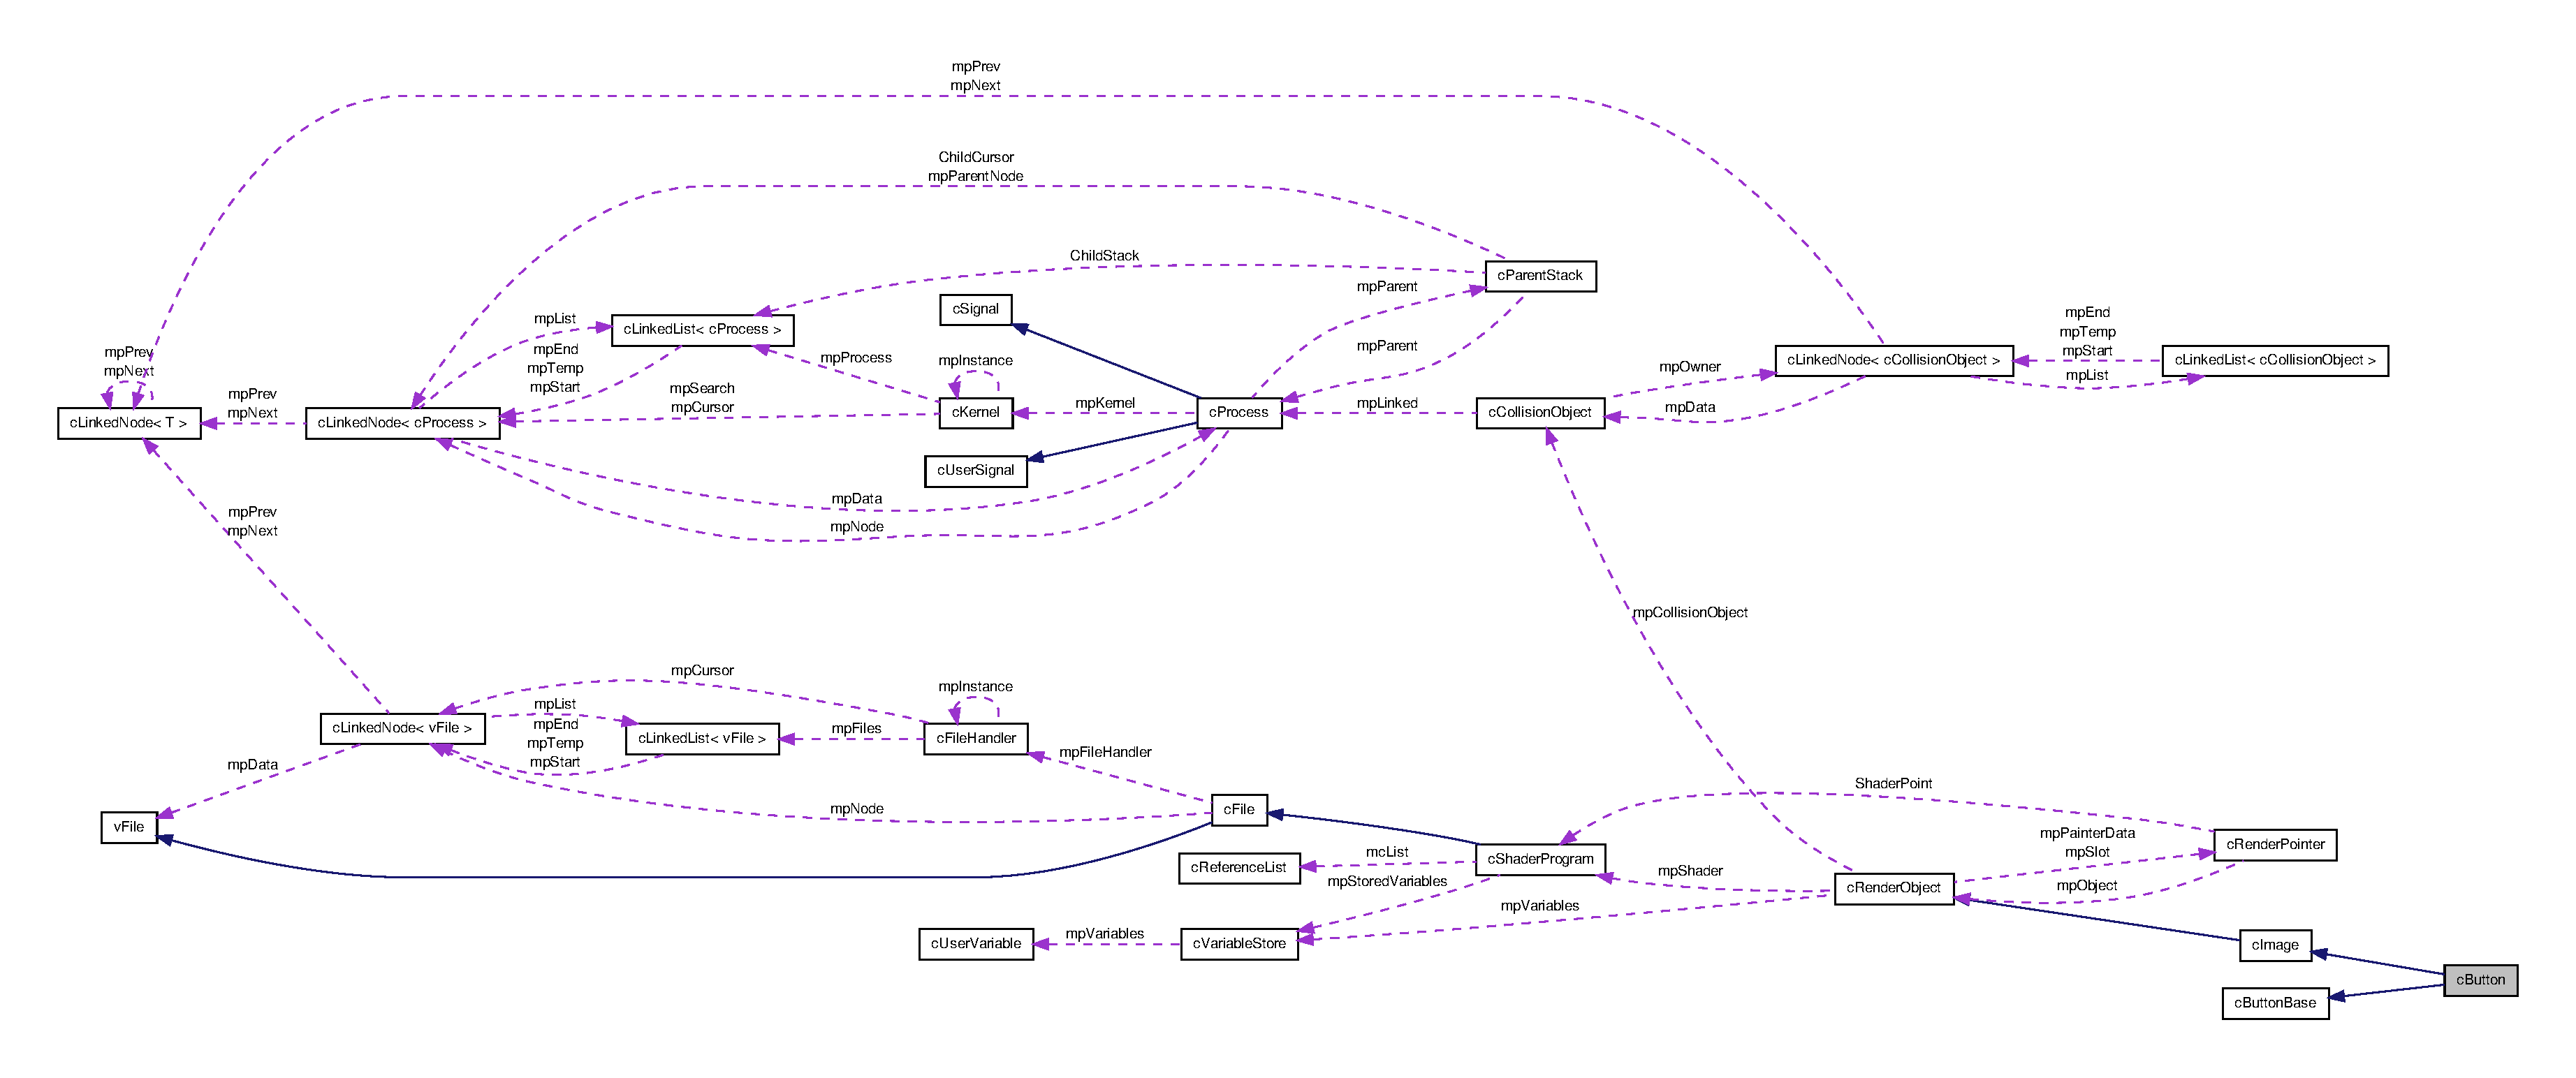
\includegraphics[width=400pt]{classc_button__coll__graph}
\end{center}
\end{figure}
\subsection*{Public Member Functions}
\begin{DoxyCompactItemize}
\item 
\hypertarget{classc_button_a3b61f8df02def1ec8ec86f4429c39022}{
void \hyperlink{classc_button_a3b61f8df02def1ec8ec86f4429c39022}{Position} (float lfX, float lfY)}
\label{classc_button_a3b61f8df02def1ec8ec86f4429c39022}

\begin{DoxyCompactList}\small\item\em Sets the Position of the Image in 2D Pixels. Measured from the center of the screen. \end{DoxyCompactList}\item 
\hypertarget{classc_button_a6b5a847fa39c2b54fa8aa93e96b34a57}{
void \hyperlink{classc_button_a6b5a847fa39c2b54fa8aa93e96b34a57}{Width} (float lfWidth)}
\label{classc_button_a6b5a847fa39c2b54fa8aa93e96b34a57}

\begin{DoxyCompactList}\small\item\em Sets the Width of the Image in Pixels to lfWidth. \end{DoxyCompactList}\item 
\hypertarget{classc_button_a30dd633ba50bf2fdb01d91129c19ce33}{
void \hyperlink{classc_button_a30dd633ba50bf2fdb01d91129c19ce33}{Height} (float lfHeight)}
\label{classc_button_a30dd633ba50bf2fdb01d91129c19ce33}

\begin{DoxyCompactList}\small\item\em Sets the Height of the Image in Pixels to lfHeight. \end{DoxyCompactList}\item 
\hypertarget{classc_button_ade80c2385df8d1c599bcdf647fa3cc42}{
void \hyperlink{classc_button_ade80c2385df8d1c599bcdf647fa3cc42}{Size} (float lfSize)}
\label{classc_button_ade80c2385df8d1c599bcdf647fa3cc42}

\begin{DoxyCompactList}\small\item\em Sets the Width of the Image in Pixels to lfSize. Will make the height the appropriate height to make the box square on screen. \end{DoxyCompactList}\end{DoxyCompactItemize}


\subsection{Detailed Description}
Renderable Button object for displaying an object as a rendered image. Takes an image and will render it as a 2D image. Will check for mouse collisions and mouse button clicks to determine how user has interacted with the button. see \hyperlink{classc_button_base}{cButtonBase} for Mouse Interaction Functions. 
\hypertarget{classc_button_base}{
\section{cButtonBase Class Reference}
\label{classc_button_base}\index{cButtonBase@{cButtonBase}}
}


Base Class for Buttons. Contains code for detecting Mouse Hover, Button is Pressed and Clicked. Contains basic code for Button functionality. See \hyperlink{classc_button}{cButton} and \hyperlink{classc_text_button}{cTextButton} for specific instances.  


\subsection*{Public Member Functions}
\begin{DoxyCompactItemize}
\item 
\hypertarget{classc_button_base_a3892d82fdc13e373d1b4474ddc0270c3}{
bool \hyperlink{classc_button_base_a3892d82fdc13e373d1b4474ddc0270c3}{Hover} ()}
\label{classc_button_base_a3892d82fdc13e373d1b4474ddc0270c3}

\begin{DoxyCompactList}\small\item\em Will return true if the mouse cursor is over this button, irrespective of whether Mouse buttons are depressed. \end{DoxyCompactList}\item 
\hypertarget{classc_button_base_ac57abb1adc326c84d2398404f9209acd}{
bool \hyperlink{classc_button_base_ac57abb1adc326c84d2398404f9209acd}{Pressed} ()}
\label{classc_button_base_ac57abb1adc326c84d2398404f9209acd}

\begin{DoxyCompactList}\small\item\em Will return true if the mouse cursor is over this button and the left mouse button is depressed. Will be updated to include all mosue buttons. \end{DoxyCompactList}\item 
\hypertarget{classc_button_base_a29e4b282201b863b55a80fd8844f39b4}{
bool \hyperlink{classc_button_base_a29e4b282201b863b55a80fd8844f39b4}{Clicked} ()}
\label{classc_button_base_a29e4b282201b863b55a80fd8844f39b4}

\begin{DoxyCompactList}\small\item\em Will return true if the user has clicked on the button and released the mouse while still over the button. Rigorous button clicking detection. Will only return true for a single frame. \end{DoxyCompactList}\end{DoxyCompactItemize}


\subsection{Detailed Description}
Base Class for Buttons. Contains code for detecting Mouse Hover, Button is Pressed and Clicked. Contains basic code for Button functionality. See \hyperlink{classc_button}{cButton} and \hyperlink{classc_text_button}{cTextButton} for specific instances. 
\hypertarget{classc_camera}{
\section{cCamera Class Reference}
\label{classc_camera}\index{cCamera@{cCamera}}
}


This class will control the rendering of the render tree. It will handle all the render objects and how to render to the screen. \hyperlink{classc_camera}{cCamera} is the renderer for a single Render List. It will contain a scene graph, and inherits \hyperlink{classc_perspective_control}{cPerspectiveControl} and \hyperlink{classc_signal}{cSignal}. It also inherits \hyperlink{classc_viewport_control}{cViewportControl} and \hyperlink{classc_camera_matrix4}{cCameraMatrix4} through \hyperlink{classc_perspective_control}{cPerspectiveControl} It can be considered as a set of renderable objects with a camera, and will render every thing in its scene graph to the screen. It will not render any objects in another cCamera's scene graph. cRenderObjects and those inheriting it can be passed a \hyperlink{classc_camera}{cCamera} as a parameter on creation to make them exist in the camera. cViewports can be created which will render the same scene graph as their owning \hyperlink{classc_camera}{cCamera} object but from another perspective. The \hyperlink{classc_camera}{cCamera} object renders first, followed by the \hyperlink{classc_viewport}{cViewport} objects in the order they were created. \hyperlink{classc_camera}{cCamera} objects can be positioned and rotated using the functions in \hyperlink{classc_camera_matrix4}{cCameraMatrix4}. The region of the screen it renders to (the viewport) is set using the functions in \hyperlink{classc_viewport_control}{cViewportControl}. The perspective (field of view etc) is set by the functions in \hyperlink{classc_perspective_control}{cPerspectiveControl}.  




Collaboration diagram for cCamera:\nopagebreak
\begin{figure}[H]
\begin{center}
\leavevmode
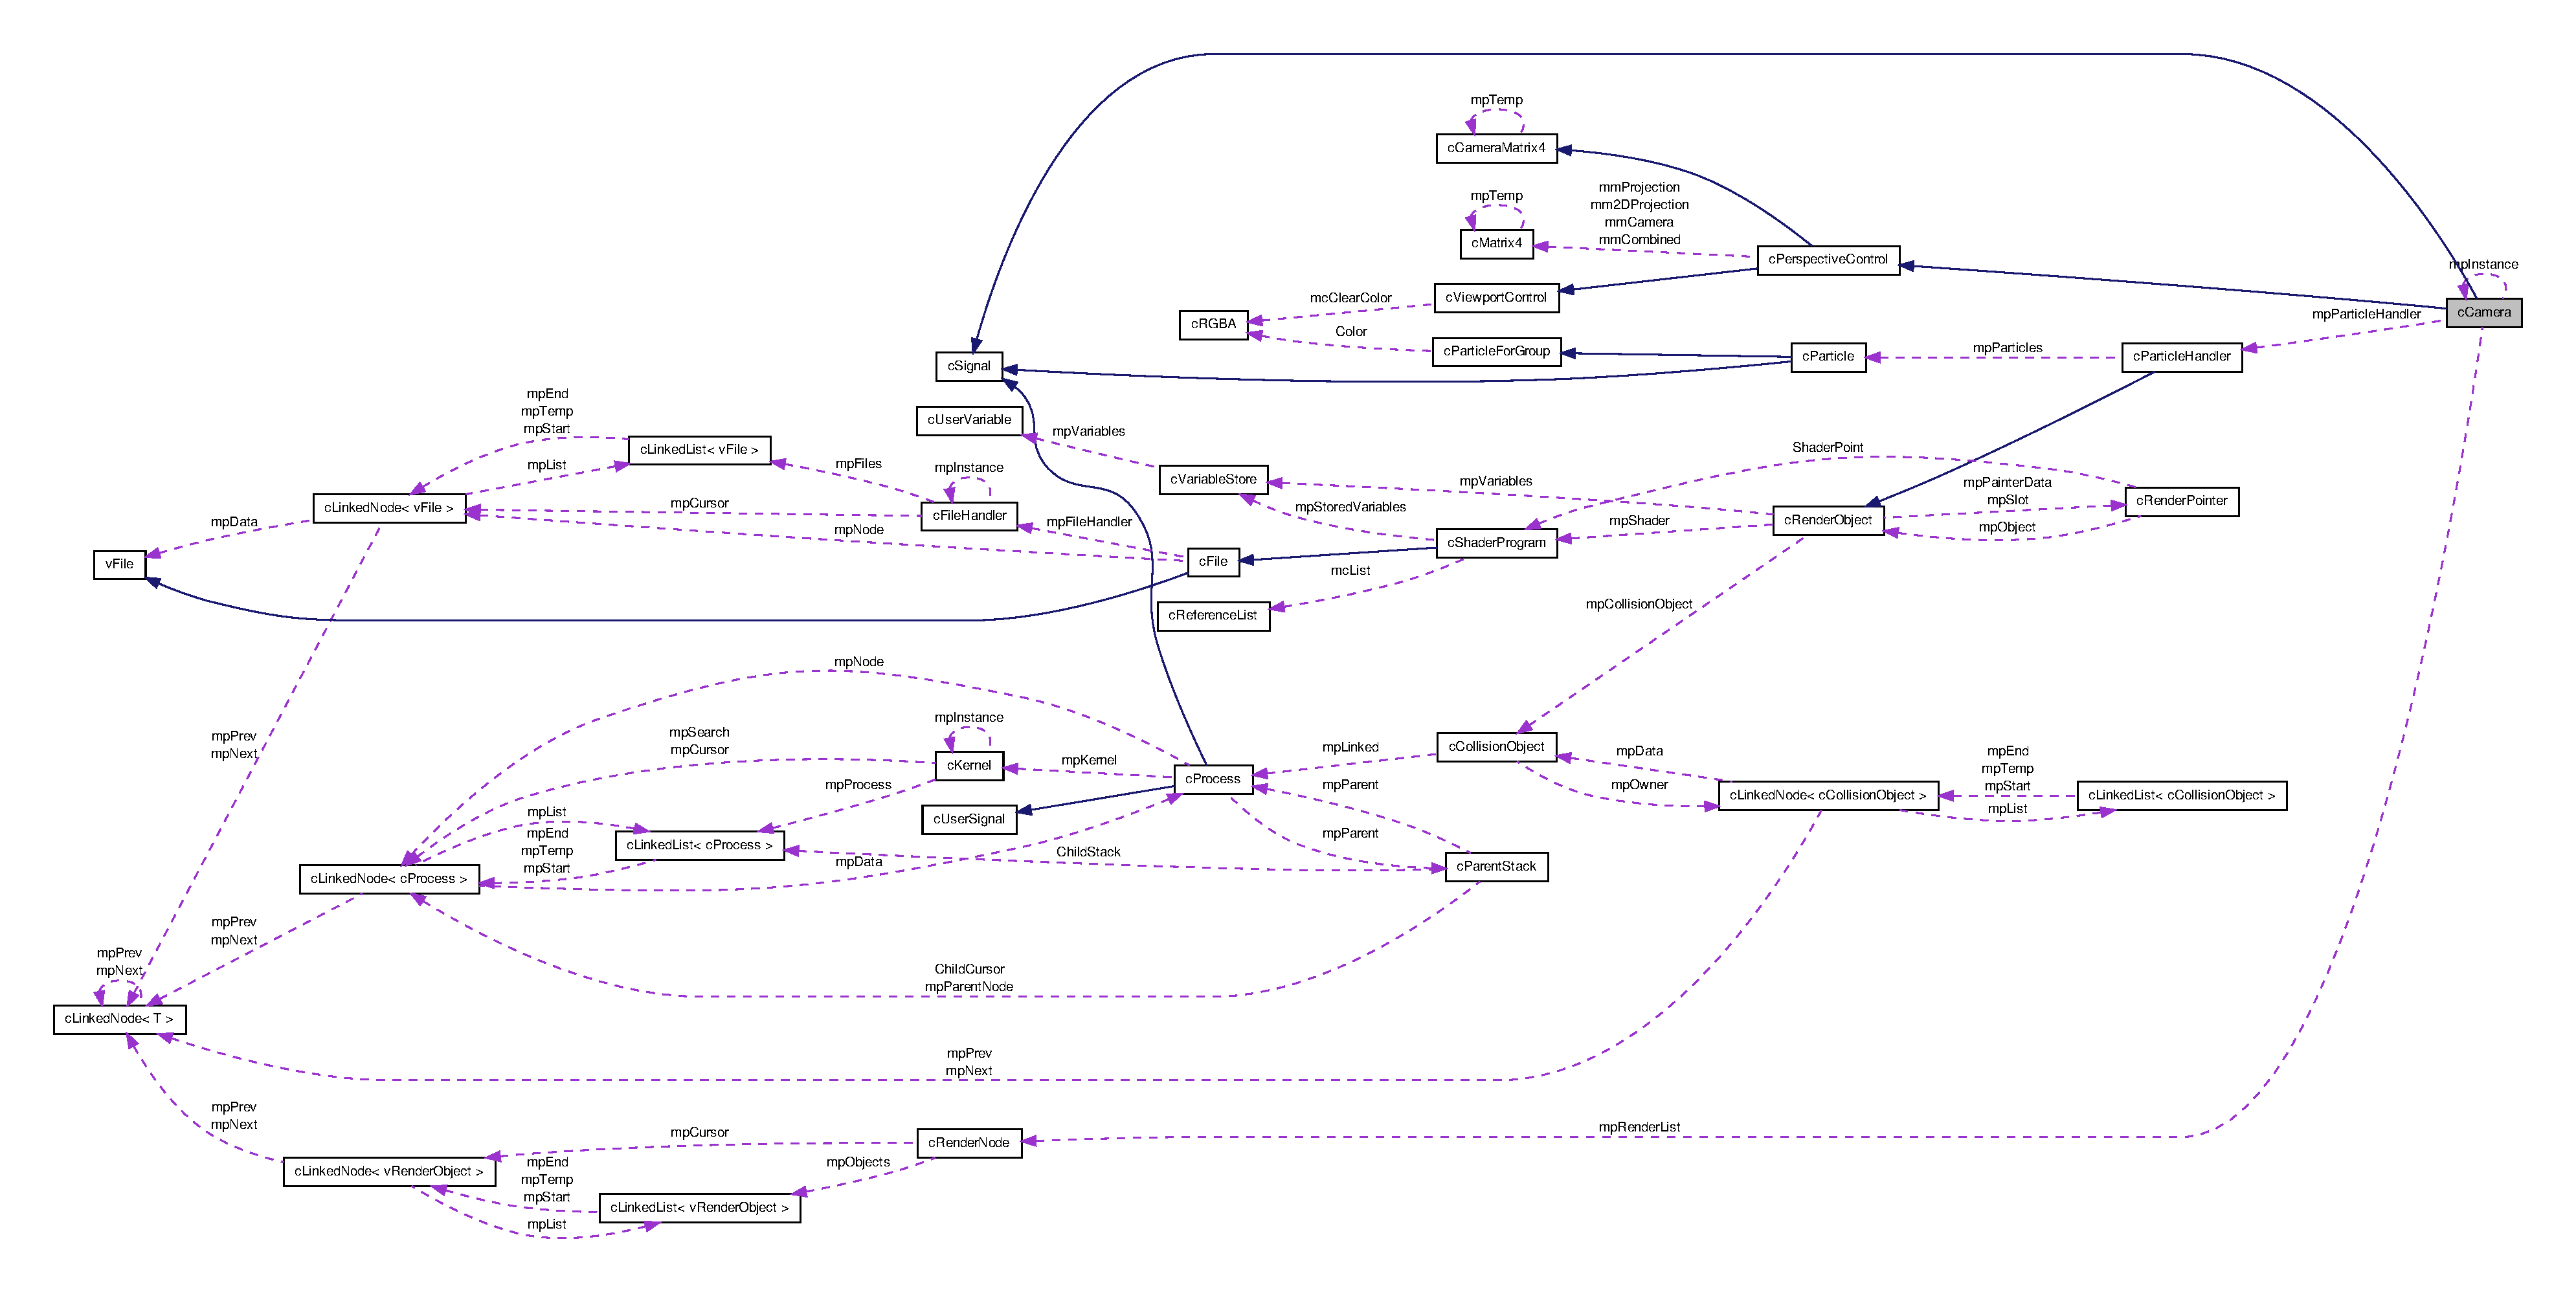
\includegraphics[width=400pt]{classc_camera__coll__graph}
\end{center}
\end{figure}
\subsection*{Public Member Functions}
\begin{DoxyCompactItemize}
\item 
\hypertarget{classc_camera_a1dbeb4e752d2a4cb50073a43c8c2132f}{
void \hyperlink{classc_camera_a1dbeb4e752d2a4cb50073a43c8c2132f}{RecalculateTotalMatrices} ()}
\label{classc_camera_a1dbeb4e752d2a4cb50073a43c8c2132f}

\begin{DoxyCompactList}\small\item\em Will recalculate all the total matrices (Projection$\ast$Camera$\ast$Global) in \hyperlink{classc_render_object}{cRenderObject} objects in this \hyperlink{classc_camera}{cCamera} objects render tree. \end{DoxyCompactList}\item 
\hypertarget{classc_camera_a4b27d2d3296c628615dc06b312459d70}{
void \hyperlink{classc_camera_a4b27d2d3296c628615dc06b312459d70}{RecalculateAllMatrices} ()}
\label{classc_camera_a4b27d2d3296c628615dc06b312459d70}

\begin{DoxyCompactList}\small\item\em Will recalculate all teh matrices in \hyperlink{classc_render_object}{cRenderObject} objects in this \hyperlink{classc_camera}{cCamera} objects render tree. \end{DoxyCompactList}\item 
\hypertarget{classc_camera_a9f2dcf74c52d7d3d0f4199b9e0d491c6}{
\hyperlink{classc_render_node}{cRenderNode} $\ast$ \hyperlink{classc_camera_a9f2dcf74c52d7d3d0f4199b9e0d491c6}{RenderList} ()}
\label{classc_camera_a9f2dcf74c52d7d3d0f4199b9e0d491c6}

\begin{DoxyCompactList}\small\item\em This will return a pointer to the scene graph. \end{DoxyCompactList}\item 
\hypertarget{classc_camera_ac63b2c284eee4b9b7182d85390279336}{
vRenderObject $\ast$ \hyperlink{classc_camera_ac63b2c284eee4b9b7182d85390279336}{vRenderList} ()}
\label{classc_camera_ac63b2c284eee4b9b7182d85390279336}

\begin{DoxyCompactList}\small\item\em This will return a virtual pointer to the the scene graph. \end{DoxyCompactList}\item 
\hypertarget{classc_camera_a6701644b2d73e607cee85dbc866ba6d9}{
void \hyperlink{classc_camera_a6701644b2d73e607cee85dbc866ba6d9}{Stop} ()}
\label{classc_camera_a6701644b2d73e607cee85dbc866ba6d9}

\begin{DoxyCompactList}\small\item\em Function for performing \hyperlink{classc_camera}{cCamera} specific actions after receiving a kill signal from via \hyperlink{classc_signal_a545074be1da41d00050bed3cd2fb2305}{cSignal::Signal(SIGNAL)}. \end{DoxyCompactList}\item 
\hypertarget{classc_camera_ab798297d6aa91192e45f7910da1e0f9b}{
\hyperlink{classc_particle_handler}{cParticleHandler} $\ast$ \hyperlink{classc_camera_ab798297d6aa91192e45f7910da1e0f9b}{ParticleHandler} ()}
\label{classc_camera_ab798297d6aa91192e45f7910da1e0f9b}

\begin{DoxyCompactList}\small\item\em Function for returning a pointer to the \hyperlink{classc_particle_handler}{cParticleHandler} for this \hyperlink{classc_camera}{cCamera}. \end{DoxyCompactList}\end{DoxyCompactItemize}
\subsection*{Static Public Member Functions}
\begin{DoxyCompactItemize}
\item 
\hypertarget{classc_camera_a06efab78c09ce37c375837242719bf58}{
static \hyperlink{classc_camera}{cCamera} $\ast$ \hyperlink{classc_camera_a06efab78c09ce37c375837242719bf58}{Instance} ()}
\label{classc_camera_a06efab78c09ce37c375837242719bf58}

\begin{DoxyCompactList}\small\item\em This function will return a pointer to the first \hyperlink{classc_camera}{cCamera} object. This can be accessed by calling tjhe macro \_\-CAMERA. \end{DoxyCompactList}\end{DoxyCompactItemize}
\subsection*{Friends}
\begin{DoxyCompactItemize}
\item 
\hypertarget{classc_camera_a36b5bd53c16eecf39974e65e00bd408e}{
class \hyperlink{classc_camera_a36b5bd53c16eecf39974e65e00bd408e}{cViewport}}
\label{classc_camera_a36b5bd53c16eecf39974e65e00bd408e}

\end{DoxyCompactItemize}


\subsection{Detailed Description}
This class will control the rendering of the render tree. It will handle all the render objects and how to render to the screen. \hyperlink{classc_camera}{cCamera} is the renderer for a single Render List. It will contain a scene graph, and inherits \hyperlink{classc_perspective_control}{cPerspectiveControl} and \hyperlink{classc_signal}{cSignal}. It also inherits \hyperlink{classc_viewport_control}{cViewportControl} and \hyperlink{classc_camera_matrix4}{cCameraMatrix4} through \hyperlink{classc_perspective_control}{cPerspectiveControl} It can be considered as a set of renderable objects with a camera, and will render every thing in its scene graph to the screen. It will not render any objects in another cCamera's scene graph. cRenderObjects and those inheriting it can be passed a \hyperlink{classc_camera}{cCamera} as a parameter on creation to make them exist in the camera. cViewports can be created which will render the same scene graph as their owning \hyperlink{classc_camera}{cCamera} object but from another perspective. The \hyperlink{classc_camera}{cCamera} object renders first, followed by the \hyperlink{classc_viewport}{cViewport} objects in the order they were created. \hyperlink{classc_camera}{cCamera} objects can be positioned and rotated using the functions in \hyperlink{classc_camera_matrix4}{cCameraMatrix4}. The region of the screen it renders to (the viewport) is set using the functions in \hyperlink{classc_viewport_control}{cViewportControl}. The perspective (field of view etc) is set by the functions in \hyperlink{classc_perspective_control}{cPerspectiveControl}. 
\hypertarget{classc_camera_handler}{
\section{cCameraHandler Class Reference}
\label{classc_camera_handler}\index{cCameraHandler@{cCameraHandler}}
}


This class is designed to own and control multiple \hyperlink{classc_camera}{cCamera} objects. All \hyperlink{classc_camera}{cCamera} objects are owned by this class. The cCameras are rendered in the order they were created and will render ontop of any previous \hyperlink{classc_camera}{cCamera} objects.  




Collaboration diagram for cCameraHandler:
\nopagebreak
\begin{figure}[H]
\begin{center}
\leavevmode
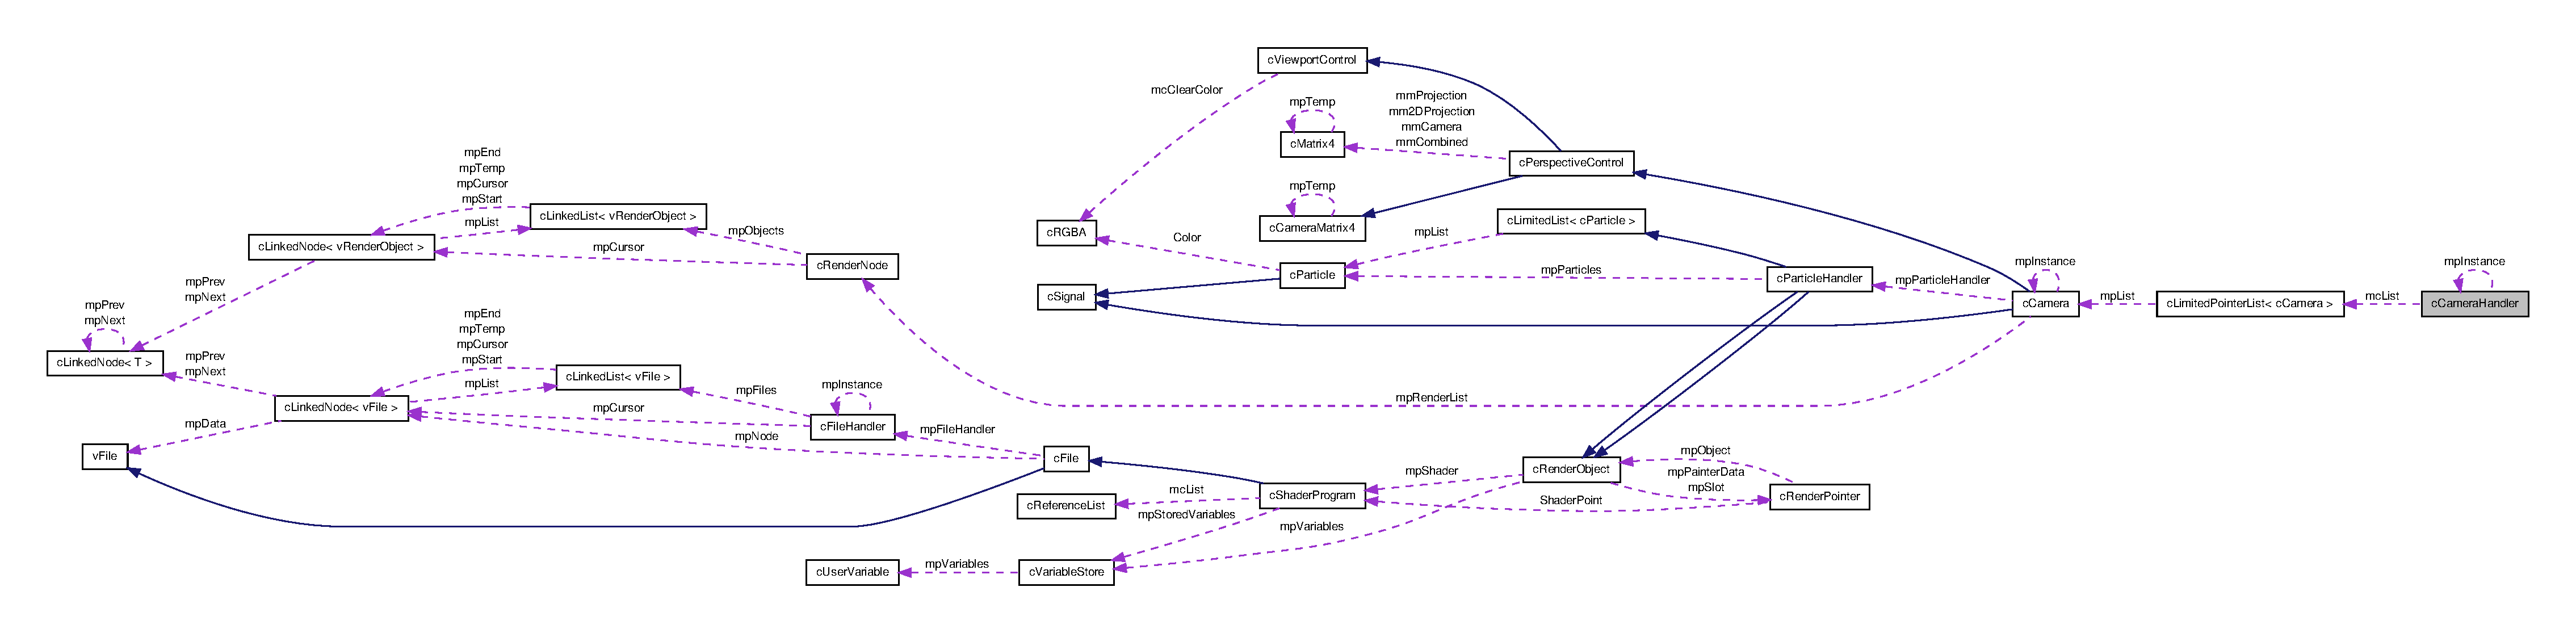
\includegraphics[width=400pt]{classc_camera_handler__coll__graph}
\end{center}
\end{figure}


\subsection{Detailed Description}
This class is designed to own and control multiple \hyperlink{classc_camera}{cCamera} objects. All \hyperlink{classc_camera}{cCamera} objects are owned by this class. The cCameras are rendered in the order they were created and will render ontop of any previous \hyperlink{classc_camera}{cCamera} objects. 
\hypertarget{classc_camera_matrix4}{
\section{cCameraMatrix4 Class Reference}
\label{classc_camera_matrix4}\index{cCameraMatrix4@{cCameraMatrix4}}
}


This is a translation matrix for a camera object. This is a translation matrix for a camera. All the translations are inverted. Distances are 'reversed', Local rotations are 'globalised' and Global roatations are 'localised'. Effectively all the translations are inverted before they are applied to this matrix.  




Inheritance diagram for cCameraMatrix4:
\nopagebreak
\begin{figure}[H]
\begin{center}
\leavevmode
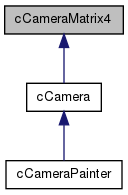
\includegraphics[width=168pt]{classc_camera_matrix4__inherit__graph}
\end{center}
\end{figure}


Collaboration diagram for cCameraMatrix4:
\nopagebreak
\begin{figure}[H]
\begin{center}
\leavevmode
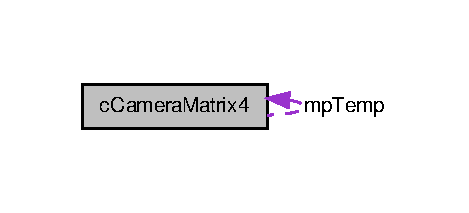
\includegraphics[width=225pt]{classc_camera_matrix4__coll__graph}
\end{center}
\end{figure}
\subsection*{Public Member Functions}
\begin{DoxyCompactItemize}
\item 
\hyperlink{classc_camera_matrix4_a99df6d312702e5474c5fedad42c95026}{cCameraMatrix4} ()
\begin{DoxyCompactList}\small\item\em This will create this matrix, and initialise all the static data for operations. \item\end{DoxyCompactList}\item 
float \hyperlink{classc_camera_matrix4_a4f3456fc67fbd37692a8daa9d11d5fc6}{Determinant} ()
\begin{DoxyCompactList}\small\item\em This will return the determinant of this matrix. \item\end{DoxyCompactList}\item 
\hyperlink{classc_camera_matrix4}{cCameraMatrix4} \hyperlink{classc_camera_matrix4_ac1fa4dd9add669a8faecd0ca79713278}{Transpose} ()
\begin{DoxyCompactList}\small\item\em This will return the transpose of this objects matrix ready for multiplications etc. \item\end{DoxyCompactList}\item 
void \hyperlink{classc_camera_matrix4_a97d111c444dd87ecec278e585fe058a7}{InvSign} ()
\begin{DoxyCompactList}\small\item\em This will make all terms of the matrix, the opposite sign to what they area. \item\end{DoxyCompactList}\item 
float $\ast$ \hyperlink{classc_camera_matrix4_ad8aad043cd8c21d5323b56cbcc90ef78}{Matrix} ()
\begin{DoxyCompactList}\small\item\em This will return a pointer to this objects matrix. \item\end{DoxyCompactList}\item 
float $\ast$ \hyperlink{classc_camera_matrix4_a89fba901320f6dda9a6b92bac09db915}{Position} ()
\begin{DoxyCompactList}\small\item\em This will return the position vector of this objects matrix. \item\end{DoxyCompactList}\item 
float \hyperlink{classc_camera_matrix4_a0133c16b734fa93e767ea89964799fb5}{X} ()
\begin{DoxyCompactList}\small\item\em This will return the X position of this objects matrix. \item\end{DoxyCompactList}\item 
float \hyperlink{classc_camera_matrix4_aec72cb78c62b2e0970824262b0b4aa1f}{Y} ()
\begin{DoxyCompactList}\small\item\em This will return the Y position of this objects matrix. \item\end{DoxyCompactList}\item 
float \hyperlink{classc_camera_matrix4_a7e3030fcedbd3b74270b26ea2b61904c}{Z} ()
\begin{DoxyCompactList}\small\item\em This will return the Z position of this objects matrix. \item\end{DoxyCompactList}\item 
void \hyperlink{classc_camera_matrix4_a23a05c1aff8a58dc662f5b871b422c17}{Identity} ()
\begin{DoxyCompactList}\small\item\em This will restore this objects matrix to an Identity matrix. \item\end{DoxyCompactList}\item 
void \hyperlink{classc_camera_matrix4_a1ec81a7ec3274f89d2b8fb94923345c0}{Zero} ()
\begin{DoxyCompactList}\small\item\em This will make the entire objects matrix equal to zero. \item\end{DoxyCompactList}\item 
\hyperlink{classc_camera_matrix4}{cCameraMatrix4} \hyperlink{classc_camera_matrix4_a975232c74548b9af68354bf6c19351d8}{operator$\ast$} (float \&lVal)
\begin{DoxyCompactList}\small\item\em This will multiplty the matrix by a float. \item\end{DoxyCompactList}\item 
\hyperlink{classc_camera_matrix4}{cCameraMatrix4} \hyperlink{classc_camera_matrix4_a41e56ee4a22ed37543c120d663e4bc3c}{operator$\ast$} (const float lVal)
\begin{DoxyCompactList}\small\item\em This will multiplty the matrix by a float. \item\end{DoxyCompactList}\item 
\hyperlink{classc_camera_matrix4}{cCameraMatrix4} \hyperlink{classc_camera_matrix4_ac3ca3f392c5046dd428cfe8cde194d37}{operator$\ast$} (\hyperlink{classc_camera_matrix4}{cCameraMatrix4} \&lVal)
\begin{DoxyCompactList}\small\item\em This will multiply this matrix by the matrix lVal. \item\end{DoxyCompactList}\item 
\hyperlink{classc_camera_matrix4}{cCameraMatrix4} $\ast$ \hyperlink{classc_camera_matrix4_a67a5947084f07eae0dd698477e1a7689}{operator$\ast$} (\hyperlink{classc_camera_matrix4}{cCameraMatrix4} $\ast$lVal)
\begin{DoxyCompactList}\small\item\em This will multiply this matrix by the matrix pointed to by lVal. \item\end{DoxyCompactList}\item 
\hyperlink{classc_camera_matrix4}{cCameraMatrix4} \hyperlink{classc_camera_matrix4_a71c4f0d6ee680f0cd511354de0033c64}{operator/} (float \&lVal)
\begin{DoxyCompactList}\small\item\em This will devide this objects matrix by the float lVal. \item\end{DoxyCompactList}\item 
\hyperlink{classc_camera_matrix4}{cCameraMatrix4} \hyperlink{classc_camera_matrix4_ab8d3c0c3df306102db000c37323692a3}{operator/} (const float lVal)
\begin{DoxyCompactList}\small\item\em This will devide this objects matrix by the float lVal. \item\end{DoxyCompactList}\item 
\hyperlink{classc_camera_matrix4}{cCameraMatrix4} \hyperlink{classc_camera_matrix4_a97ada5a5b0698d4e8f383754f30cbd2b}{operator+} (float \&lVal)
\begin{DoxyCompactList}\small\item\em This will add lVal to this objects matrix. lVal is added to every position in the matrix. \item\end{DoxyCompactList}\item 
\hyperlink{classc_camera_matrix4}{cCameraMatrix4} \hyperlink{classc_camera_matrix4_adb619821208a735d6fd262770d0dbf8a}{operator+} (const float lVal)
\begin{DoxyCompactList}\small\item\em This will add lVal to this objects matrix. lVal is added to every position in the matrix. \item\end{DoxyCompactList}\item 
\hyperlink{classc_camera_matrix4}{cCameraMatrix4} \hyperlink{classc_camera_matrix4_a4456564f6c57e7a9072ab31c242bef49}{operator+} (\hyperlink{classc_camera_matrix4}{cCameraMatrix4} \&lVal)
\begin{DoxyCompactList}\small\item\em This will add this objects matrix and the matrix lVal. \item\end{DoxyCompactList}\item 
\hyperlink{classc_camera_matrix4}{cCameraMatrix4} \hyperlink{classc_camera_matrix4_a42eb30055c9b58f2fc3fabf8201e7929}{operator-\/} (float \&lVal)
\begin{DoxyCompactList}\small\item\em This will deduct lVal from this objects matrix. lVal is deducted from every position in the matrix. \item\end{DoxyCompactList}\item 
\hyperlink{classc_camera_matrix4}{cCameraMatrix4} \hyperlink{classc_camera_matrix4_a3f13c8e5f71d9c158332fe87a49f1b61}{operator-\/} (const float lVal)
\begin{DoxyCompactList}\small\item\em This will deduct lVal from this objects matrix. lVal is deducted from every position in the matrix. \item\end{DoxyCompactList}\item 
\hyperlink{classc_camera_matrix4}{cCameraMatrix4} \hyperlink{classc_camera_matrix4_a97c7f6820b87ea9a217c4412e0c89e49}{operator-\/} (\hyperlink{classc_camera_matrix4}{cCameraMatrix4} \&lVal)
\begin{DoxyCompactList}\small\item\em This will deduct the matrix lVal from this objects matrix. \item\end{DoxyCompactList}\item 
float \& \hyperlink{classc_camera_matrix4_a57bce39e1e5ff464edd9dd1c32fcdd3b}{operator\mbox{[}$\,$\mbox{]}} (uint16 liPos)
\begin{DoxyCompactList}\small\item\em This will return the float in the position liPos in this objects matrix. \item\end{DoxyCompactList}\item 
float \& \hyperlink{classc_camera_matrix4_aeae4d353c1153e9eb15461eac399a29f}{operator()} (uint16 liColumn, uint16 liRow)
\begin{DoxyCompactList}\small\item\em This will return the float in the position \mbox{[}liColumn,liRow\mbox{]} in this objects matrix. \item\end{DoxyCompactList}\item 
float \hyperlink{classc_camera_matrix4_a21020ff4493a379b107a98c8a699d5f7}{operator=} (float \&lVal)
\begin{DoxyCompactList}\small\item\em This will set every float in this objects matrix to lVal. \item\end{DoxyCompactList}\item 
float \hyperlink{classc_camera_matrix4_a13c2e801ef13951525908a0985cf2ba7}{operator=} (const float lVal)
\begin{DoxyCompactList}\small\item\em This will set every float in this objects matrix to lVal. \item\end{DoxyCompactList}\item 
\hyperlink{classc_camera_matrix4}{cCameraMatrix4} \hyperlink{classc_camera_matrix4_a570900cf46a3c6e8a31e957a4dd24103}{operator=} (\hyperlink{classc_camera_matrix4}{cCameraMatrix4} \&lVal)
\begin{DoxyCompactList}\small\item\em This will set this objects matrix to be the same as the matrix lVal. \item\end{DoxyCompactList}\item 
\hyperlink{classc_camera_matrix4}{cCameraMatrix4} $\ast$ \hyperlink{classc_camera_matrix4_aabdb9adddb777e59ae8594cb62b0e02e}{operator=} (\hyperlink{classc_camera_matrix4}{cCameraMatrix4} $\ast$lVal)
\begin{DoxyCompactList}\small\item\em This will set this objects matrix to be the same as the matrix lVal. \item\end{DoxyCompactList}\item 
void \hyperlink{classc_camera_matrix4_a62fa2879539cc733e661d02b8a898578}{Position} (\hyperlink{classc2_d_vf}{c2DVf} $\ast$lpPosition)
\begin{DoxyCompactList}\small\item\em This will set this objects matrix position (2D -\/ X,Y) vector to be the same as lpPosition. \item\end{DoxyCompactList}\item 
void \hyperlink{classc_camera_matrix4_a293ac7d2919eae7205b568ea56fa104c}{Position} (float lfX, float lfY)
\begin{DoxyCompactList}\small\item\em This will set this objects matrix position vector to be lfX,lfY. \item\end{DoxyCompactList}\item 
void \hyperlink{classc_camera_matrix4_a7110b0f3aa924a2cfefe8ca149e0b41f}{Position} (\hyperlink{classc3_d_vf}{c3DVf} $\ast$lpPosition)
\begin{DoxyCompactList}\small\item\em This will set this objects matrix position vector to be the same as lpPosition. \item\end{DoxyCompactList}\item 
void \hyperlink{classc_camera_matrix4_a1aa471464a30ce27fe339b743b840516}{Position} (float lfX, float lfY, float lfZ)
\begin{DoxyCompactList}\small\item\em This will set this objects matrix position vector to be lfX,lfY,lfZ. \item\end{DoxyCompactList}\item 
void \hyperlink{classc_camera_matrix4_af130ddef040458f01b9a2365f41c567a}{PositionX} (float lfX)
\begin{DoxyCompactList}\small\item\em This will set this objects X position to he lfX. \item\end{DoxyCompactList}\item 
void \hyperlink{classc_camera_matrix4_adce3f6365faf3af907994f50c004c736}{PositionY} (float lfY)
\begin{DoxyCompactList}\small\item\em This will set this objects Y position to he lfY. \item\end{DoxyCompactList}\item 
void \hyperlink{classc_camera_matrix4_a6ea814a92ce2d7fcc1ba66490127b2f2}{PositionZ} (float lfZ)
\begin{DoxyCompactList}\small\item\em This will set this objects Z position to he lfZ. \item\end{DoxyCompactList}\item 
void \hyperlink{classc_camera_matrix4_a4a07cdf5cb578378193487a1ac304380}{AdvanceX} (float lfDistance)
\begin{DoxyCompactList}\small\item\em This will advance the position of this objects X position by lfDistance along local axis. \item\end{DoxyCompactList}\item 
void \hyperlink{classc_camera_matrix4_a1c644144c6673fad0d45ac2a28065edb}{AdvanceY} (float lfDistance)
\begin{DoxyCompactList}\small\item\em This will advance the position of this objects Y position by lfDistance along local axis. \item\end{DoxyCompactList}\item 
void \hyperlink{classc_camera_matrix4_a18915056c461b31b5ea916715fa2582f}{AdvanceZ} (float lfDistance)
\begin{DoxyCompactList}\small\item\em This will advance the position of this objects Z position by lfDistance along local axis. \item\end{DoxyCompactList}\item 
void \hyperlink{classc_camera_matrix4_acd0e691c270f18c80965bf8da4442d5b}{Advance} (float lfX, float lfY, float lfZ)
\begin{DoxyCompactList}\small\item\em This will advance the position of this objects X,Y and Z positions by lfX,lfY and lfZ along local axis. \item\end{DoxyCompactList}\item 
void \hyperlink{classc_camera_matrix4_a69ef5c53bd239d2f1041ac9330c2cc08}{GAdvanceX} (float lfDistance)
\begin{DoxyCompactList}\small\item\em This will advance the position of this objects X position by lfDistance along global axis. \item\end{DoxyCompactList}\item 
void \hyperlink{classc_camera_matrix4_a7cb5d64085acdcc74dcad1e965a52b3b}{GAdvanceY} (float lfDistance)
\begin{DoxyCompactList}\small\item\em This will advance the position of this objects Y position by lfDistance along global axis. \item\end{DoxyCompactList}\item 
void \hyperlink{classc_camera_matrix4_afd68814e78dd2ffaec2f9bc4289aca36}{GAdvanceZ} (float lfDistance)
\begin{DoxyCompactList}\small\item\em This will advance the position of this objects Z position by lfDistance along global axis. \item\end{DoxyCompactList}\item 
void \hyperlink{classc_camera_matrix4_a342b888f43a65b6c4a14b818c2519157}{GAdvance} (float lfX, float lfY, float lfZ)
\begin{DoxyCompactList}\small\item\em This will advance the position of this objects X,Y and Z positions by lfX,lfY and lfZ along global axis. \item\end{DoxyCompactList}\item 
void \hyperlink{classc_camera_matrix4_ab9ea2ea9b429824586d4fa74e709426e}{LRotate} (float lfAngle)
\begin{DoxyCompactList}\small\item\em This will localy rotate the object by lfAngle radians about the Z axis. This is suitable to be used by 2D objects. \item\end{DoxyCompactList}\item 
void \hyperlink{classc_camera_matrix4_a08ffa3e8e4622821ba80aaa51300e645}{LRotateX} (float lfAngle)
\begin{DoxyCompactList}\small\item\em This will rotate the object by lfAngle radians about its local X axis. This is suitable for use by 3D objects. \item\end{DoxyCompactList}\item 
void \hyperlink{classc_camera_matrix4_a369f1a97e289850afffd03302bb5bd0f}{LRotateY} (float lfAngle)
\begin{DoxyCompactList}\small\item\em This will rotate the object by lfAngle radians about its local Y axis. This is suitable for use by 3D objects. \item\end{DoxyCompactList}\item 
void \hyperlink{classc_camera_matrix4_ad4574f0b96ef29472ca6a286f4d8204d}{LRotateZ} (float lfAngle)
\begin{DoxyCompactList}\small\item\em This will rotate the object by lfAngle radians about its local Z axis. This is suitable for use by 3D objects. \item\end{DoxyCompactList}\item 
void \hyperlink{classc_camera_matrix4_a09c8d44629bf63643c8f09ccdc2294bc}{GRotateX} (float lfAngle)
\begin{DoxyCompactList}\small\item\em This will rotate the object by lfAngle radians about its global X axis. This is suitable for use by 3D objects. \item\end{DoxyCompactList}\item 
void \hyperlink{classc_camera_matrix4_a48eb5374c0e7fa4eca25f48a6411052d}{GRotateY} (float lfAngle)
\begin{DoxyCompactList}\small\item\em This will rotate the object by lfAngle radians about its global Y axis. This is suitable for use by 3D objects. \item\end{DoxyCompactList}\item 
void \hyperlink{classc_camera_matrix4_a993d7410719b1fd7d871f728527a3947}{GRotateZ} (float lfAngle)
\begin{DoxyCompactList}\small\item\em This will rotate the object by lfAngle radians about its global Z axis. This is suitable for use by 3D objects. \item\end{DoxyCompactList}\item 
void \hyperlink{classc_camera_matrix4_a2fc16f6a7aa3ffec1317f71645aa857b}{GRotateX} (float lfAngle, float lfX, float lfY, float lfZ)
\begin{DoxyCompactList}\small\item\em This will rotate the object by lfAngle radians about the global X axis of the point lfX,lfY,lfZ. This is suitable for use by 3D objects. \item\end{DoxyCompactList}\item 
void \hyperlink{classc_camera_matrix4_a775326e51bf492340e8768d219a4e5e2}{GRotateY} (float lfAngle, float lfX, float lfY, float lfZ)
\begin{DoxyCompactList}\small\item\em This will rotate the object by lfAngle radians about the global Y axis of the point lfX,lfY,lfZ. This is suitable for use by 3D objects. \item\end{DoxyCompactList}\item 
void \hyperlink{classc_camera_matrix4_a8c99ce20f8594e9a66e0a7b2830ec9e9}{GRotateZ} (float lfAngle, float lfX, float lfY, float lfZ)
\begin{DoxyCompactList}\small\item\em This will rotate the object by lfAngle radians about the global Z axis of the point lfX,lfY,lfZ. This is suitable for use by 3D objects. \item\end{DoxyCompactList}\item 
void \hyperlink{classc_camera_matrix4_a6be0f1f82cc4ee5a5953cb3b569b4285}{Angle} (float lfAngle)
\begin{DoxyCompactList}\small\item\em This will set the current objects matrix to be rotated to the absolute angle lfAngle. This is suitable for 2D objects. \item\end{DoxyCompactList}\item 
void \hyperlink{classc_camera_matrix4_a620ba52edfd711f011d43a441eece9bc}{Resize} (float lfScale)
\begin{DoxyCompactList}\small\item\em This will scale this objects matrix by a factor of lfScale. \item\end{DoxyCompactList}\item 
void \hyperlink{classc_camera_matrix4_a53c3d81781d403c9bf9671879f79a838}{LResizeX} (float lfScale)
\begin{DoxyCompactList}\small\item\em This will scale this objects local X axis by a factor of lfScale. \item\end{DoxyCompactList}\item 
void \hyperlink{classc_camera_matrix4_a12eda8948b16c1a2818093016d8ef755}{LResizeY} (float lfScale)
\begin{DoxyCompactList}\small\item\em This will scale this objects local Y axis by a factor of lfScale. \item\end{DoxyCompactList}\item 
void \hyperlink{classc_camera_matrix4_a6f1fbcfe585f86002cb586eab9df7c7d}{LResizeZ} (float lfScale)
\begin{DoxyCompactList}\small\item\em This will scale this objects local Z axis by a factor of lfScale. \item\end{DoxyCompactList}\item 
void \hyperlink{classc_camera_matrix4_a9984a8427cd90e77a2fb6462ecf99ecc}{GResizeX} (float lfScale)
\begin{DoxyCompactList}\small\item\em This will scale this objects globally along the X axis by a factor of lfScale. \item\end{DoxyCompactList}\item 
void \hyperlink{classc_camera_matrix4_aa2a9326b7f2a6f00aa5b45057c69ecd3}{GResizeY} (float lfScale)
\begin{DoxyCompactList}\small\item\em This will scale this objects globally along the Y axis by a factor of lfScale. \item\end{DoxyCompactList}\item 
void \hyperlink{classc_camera_matrix4_a1ab7808cf06ddf7ec373b926c77f85c6}{GResizeZ} (float lfScale)
\begin{DoxyCompactList}\small\item\em This will scale this objects globally along the Z axis by a factor of lfScale. \item\end{DoxyCompactList}\item 
uint32 \hyperlink{classc_camera_matrix4_adf5481b8c761008b9611e0b071e70914}{Distance3D} (float $\ast$lpOther)
\begin{DoxyCompactList}\small\item\em This will return the 3D distance between this matrix and the matrix pointed to by lpOther. \item\end{DoxyCompactList}\item 
uint32 \hyperlink{classc_camera_matrix4_a02c68197ed3c64c95985269f5b9f66a4}{Distance2D} (float $\ast$lpOther)
\begin{DoxyCompactList}\small\item\em This will return the 2D distance between this matrix and the matrix pointed to by lpOther. \item\end{DoxyCompactList}\item 
void \hyperlink{classc_camera_matrix4_aeee787e0f5895a613e8be9efbade408f}{Follow} (\hyperlink{classc_matrix4}{cMatrix4} $\ast$lpOther, float lfDist)
\item 
void \hyperlink{classc_camera_matrix4_aa8ca47d59f6b3b454d700329bdbbdeea}{PointAt} (float $\ast$mpPos)
\end{DoxyCompactItemize}
\subsection*{Public Attributes}
\begin{DoxyCompactItemize}
\item 
float \hyperlink{classc_camera_matrix4_afb48ac51e480abcece16e031d8bc300a}{mpPosition} \mbox{[}3\mbox{]}
\begin{DoxyCompactList}\small\item\em The position of this matrix has been seperated from the rest of the matrix as the camera should rotate around 0,0,0, not itself? \item\end{DoxyCompactList}\end{DoxyCompactItemize}


\subsection{Detailed Description}
This is a translation matrix for a camera object. This is a translation matrix for a camera. All the translations are inverted. Distances are 'reversed', Local rotations are 'globalised' and Global roatations are 'localised'. Effectively all the translations are inverted before they are applied to this matrix. 

Definition at line 10 of file WTcCameraMatrix4.h.



\subsection{Constructor \& Destructor Documentation}
\hypertarget{classc_camera_matrix4_a99df6d312702e5474c5fedad42c95026}{
\index{cCameraMatrix4@{cCameraMatrix4}!cCameraMatrix4@{cCameraMatrix4}}
\index{cCameraMatrix4@{cCameraMatrix4}!cCameraMatrix4@{cCameraMatrix4}}
\subsubsection[{cCameraMatrix4}]{\setlength{\rightskip}{0pt plus 5cm}cCameraMatrix4::cCameraMatrix4 (
\begin{DoxyParamCaption}
{}
\end{DoxyParamCaption}
)}}
\label{classc_camera_matrix4_a99df6d312702e5474c5fedad42c95026}


This will create this matrix, and initialise all the static data for operations. 



Definition at line 9 of file WTcCameraMatrix4.cpp.



\subsection{Member Function Documentation}
\hypertarget{classc_camera_matrix4_acd0e691c270f18c80965bf8da4442d5b}{
\index{cCameraMatrix4@{cCameraMatrix4}!Advance@{Advance}}
\index{Advance@{Advance}!cCameraMatrix4@{cCameraMatrix4}}
\subsubsection[{Advance}]{\setlength{\rightskip}{0pt plus 5cm}void cCameraMatrix4::Advance (
\begin{DoxyParamCaption}
\item[{float}]{lfX, }
\item[{float}]{lfY, }
\item[{float}]{lfZ}
\end{DoxyParamCaption}
)}}
\label{classc_camera_matrix4_acd0e691c270f18c80965bf8da4442d5b}


This will advance the position of this objects X,Y and Z positions by lfX,lfY and lfZ along local axis. 



Definition at line 742 of file WTcCameraMatrix4.cpp.

\hypertarget{classc_camera_matrix4_a4a07cdf5cb578378193487a1ac304380}{
\index{cCameraMatrix4@{cCameraMatrix4}!AdvanceX@{AdvanceX}}
\index{AdvanceX@{AdvanceX}!cCameraMatrix4@{cCameraMatrix4}}
\subsubsection[{AdvanceX}]{\setlength{\rightskip}{0pt plus 5cm}void cCameraMatrix4::AdvanceX (
\begin{DoxyParamCaption}
\item[{float}]{lfDistance}
\end{DoxyParamCaption}
)}}
\label{classc_camera_matrix4_a4a07cdf5cb578378193487a1ac304380}


This will advance the position of this objects X position by lfDistance along local axis. 



Definition at line 720 of file WTcCameraMatrix4.cpp.

\hypertarget{classc_camera_matrix4_a1c644144c6673fad0d45ac2a28065edb}{
\index{cCameraMatrix4@{cCameraMatrix4}!AdvanceY@{AdvanceY}}
\index{AdvanceY@{AdvanceY}!cCameraMatrix4@{cCameraMatrix4}}
\subsubsection[{AdvanceY}]{\setlength{\rightskip}{0pt plus 5cm}void cCameraMatrix4::AdvanceY (
\begin{DoxyParamCaption}
\item[{float}]{lfDistance}
\end{DoxyParamCaption}
)}}
\label{classc_camera_matrix4_a1c644144c6673fad0d45ac2a28065edb}


This will advance the position of this objects Y position by lfDistance along local axis. 



Definition at line 727 of file WTcCameraMatrix4.cpp.

\hypertarget{classc_camera_matrix4_a18915056c461b31b5ea916715fa2582f}{
\index{cCameraMatrix4@{cCameraMatrix4}!AdvanceZ@{AdvanceZ}}
\index{AdvanceZ@{AdvanceZ}!cCameraMatrix4@{cCameraMatrix4}}
\subsubsection[{AdvanceZ}]{\setlength{\rightskip}{0pt plus 5cm}void cCameraMatrix4::AdvanceZ (
\begin{DoxyParamCaption}
\item[{float}]{lfDistance}
\end{DoxyParamCaption}
)}}
\label{classc_camera_matrix4_a18915056c461b31b5ea916715fa2582f}


This will advance the position of this objects Z position by lfDistance along local axis. 



Definition at line 734 of file WTcCameraMatrix4.cpp.

\hypertarget{classc_camera_matrix4_a6be0f1f82cc4ee5a5953cb3b569b4285}{
\index{cCameraMatrix4@{cCameraMatrix4}!Angle@{Angle}}
\index{Angle@{Angle}!cCameraMatrix4@{cCameraMatrix4}}
\subsubsection[{Angle}]{\setlength{\rightskip}{0pt plus 5cm}void cCameraMatrix4::Angle (
\begin{DoxyParamCaption}
\item[{float}]{lfAngle}
\end{DoxyParamCaption}
)}}
\label{classc_camera_matrix4_a6be0f1f82cc4ee5a5953cb3b569b4285}


This will set the current objects matrix to be rotated to the absolute angle lfAngle. This is suitable for 2D objects. 



Definition at line 513 of file WTcCameraMatrix4.cpp.

\hypertarget{classc_camera_matrix4_a4f3456fc67fbd37692a8daa9d11d5fc6}{
\index{cCameraMatrix4@{cCameraMatrix4}!Determinant@{Determinant}}
\index{Determinant@{Determinant}!cCameraMatrix4@{cCameraMatrix4}}
\subsubsection[{Determinant}]{\setlength{\rightskip}{0pt plus 5cm}float cCameraMatrix4::Determinant (
\begin{DoxyParamCaption}
{}
\end{DoxyParamCaption}
)}}
\label{classc_camera_matrix4_a4f3456fc67fbd37692a8daa9d11d5fc6}


This will return the determinant of this matrix. 



Definition at line 350 of file WTcCameraMatrix4.cpp.

\hypertarget{classc_camera_matrix4_a02c68197ed3c64c95985269f5b9f66a4}{
\index{cCameraMatrix4@{cCameraMatrix4}!Distance2D@{Distance2D}}
\index{Distance2D@{Distance2D}!cCameraMatrix4@{cCameraMatrix4}}
\subsubsection[{Distance2D}]{\setlength{\rightskip}{0pt plus 5cm}uint32 cCameraMatrix4::Distance2D (
\begin{DoxyParamCaption}
\item[{float $\ast$}]{lpOther}
\end{DoxyParamCaption}
)}}
\label{classc_camera_matrix4_a02c68197ed3c64c95985269f5b9f66a4}


This will return the 2D distance between this matrix and the matrix pointed to by lpOther. 



Definition at line 861 of file WTcCameraMatrix4.cpp.

\hypertarget{classc_camera_matrix4_adf5481b8c761008b9611e0b071e70914}{
\index{cCameraMatrix4@{cCameraMatrix4}!Distance3D@{Distance3D}}
\index{Distance3D@{Distance3D}!cCameraMatrix4@{cCameraMatrix4}}
\subsubsection[{Distance3D}]{\setlength{\rightskip}{0pt plus 5cm}uint32 cCameraMatrix4::Distance3D (
\begin{DoxyParamCaption}
\item[{float $\ast$}]{lpOther}
\end{DoxyParamCaption}
)}}
\label{classc_camera_matrix4_adf5481b8c761008b9611e0b071e70914}


This will return the 3D distance between this matrix and the matrix pointed to by lpOther. 



Definition at line 852 of file WTcCameraMatrix4.cpp.

\hypertarget{classc_camera_matrix4_aeee787e0f5895a613e8be9efbade408f}{
\index{cCameraMatrix4@{cCameraMatrix4}!Follow@{Follow}}
\index{Follow@{Follow}!cCameraMatrix4@{cCameraMatrix4}}
\subsubsection[{Follow}]{\setlength{\rightskip}{0pt plus 5cm}void cCameraMatrix4::Follow (
\begin{DoxyParamCaption}
\item[{{\bf cMatrix4} $\ast$}]{lpOther, }
\item[{float}]{lfDist}
\end{DoxyParamCaption}
)}}
\label{classc_camera_matrix4_aeee787e0f5895a613e8be9efbade408f}


Definition at line 869 of file WTcCameraMatrix4.cpp.

\hypertarget{classc_camera_matrix4_a342b888f43a65b6c4a14b818c2519157}{
\index{cCameraMatrix4@{cCameraMatrix4}!GAdvance@{GAdvance}}
\index{GAdvance@{GAdvance}!cCameraMatrix4@{cCameraMatrix4}}
\subsubsection[{GAdvance}]{\setlength{\rightskip}{0pt plus 5cm}void cCameraMatrix4::GAdvance (
\begin{DoxyParamCaption}
\item[{float}]{lfX, }
\item[{float}]{lfY, }
\item[{float}]{lfZ}
\end{DoxyParamCaption}
)}}
\label{classc_camera_matrix4_a342b888f43a65b6c4a14b818c2519157}


This will advance the position of this objects X,Y and Z positions by lfX,lfY and lfZ along global axis. 



Definition at line 758 of file WTcCameraMatrix4.cpp.

\hypertarget{classc_camera_matrix4_a69ef5c53bd239d2f1041ac9330c2cc08}{
\index{cCameraMatrix4@{cCameraMatrix4}!GAdvanceX@{GAdvanceX}}
\index{GAdvanceX@{GAdvanceX}!cCameraMatrix4@{cCameraMatrix4}}
\subsubsection[{GAdvanceX}]{\setlength{\rightskip}{0pt plus 5cm}void cCameraMatrix4::GAdvanceX (
\begin{DoxyParamCaption}
\item[{float}]{lfDistance}
\end{DoxyParamCaption}
)}}
\label{classc_camera_matrix4_a69ef5c53bd239d2f1041ac9330c2cc08}


This will advance the position of this objects X position by lfDistance along global axis. 



Definition at line 749 of file WTcCameraMatrix4.cpp.

\hypertarget{classc_camera_matrix4_a7cb5d64085acdcc74dcad1e965a52b3b}{
\index{cCameraMatrix4@{cCameraMatrix4}!GAdvanceY@{GAdvanceY}}
\index{GAdvanceY@{GAdvanceY}!cCameraMatrix4@{cCameraMatrix4}}
\subsubsection[{GAdvanceY}]{\setlength{\rightskip}{0pt plus 5cm}void cCameraMatrix4::GAdvanceY (
\begin{DoxyParamCaption}
\item[{float}]{lfDistance}
\end{DoxyParamCaption}
)}}
\label{classc_camera_matrix4_a7cb5d64085acdcc74dcad1e965a52b3b}


This will advance the position of this objects Y position by lfDistance along global axis. 



Definition at line 752 of file WTcCameraMatrix4.cpp.

\hypertarget{classc_camera_matrix4_afd68814e78dd2ffaec2f9bc4289aca36}{
\index{cCameraMatrix4@{cCameraMatrix4}!GAdvanceZ@{GAdvanceZ}}
\index{GAdvanceZ@{GAdvanceZ}!cCameraMatrix4@{cCameraMatrix4}}
\subsubsection[{GAdvanceZ}]{\setlength{\rightskip}{0pt plus 5cm}void cCameraMatrix4::GAdvanceZ (
\begin{DoxyParamCaption}
\item[{float}]{lfDistance}
\end{DoxyParamCaption}
)}}
\label{classc_camera_matrix4_afd68814e78dd2ffaec2f9bc4289aca36}


This will advance the position of this objects Z position by lfDistance along global axis. 



Definition at line 755 of file WTcCameraMatrix4.cpp.

\hypertarget{classc_camera_matrix4_a9984a8427cd90e77a2fb6462ecf99ecc}{
\index{cCameraMatrix4@{cCameraMatrix4}!GResizeX@{GResizeX}}
\index{GResizeX@{GResizeX}!cCameraMatrix4@{cCameraMatrix4}}
\subsubsection[{GResizeX}]{\setlength{\rightskip}{0pt plus 5cm}void cCameraMatrix4::GResizeX (
\begin{DoxyParamCaption}
\item[{float}]{lfScale}
\end{DoxyParamCaption}
)}}
\label{classc_camera_matrix4_a9984a8427cd90e77a2fb6462ecf99ecc}


This will scale this objects globally along the X axis by a factor of lfScale. 



Definition at line 637 of file WTcCameraMatrix4.cpp.

\hypertarget{classc_camera_matrix4_aa2a9326b7f2a6f00aa5b45057c69ecd3}{
\index{cCameraMatrix4@{cCameraMatrix4}!GResizeY@{GResizeY}}
\index{GResizeY@{GResizeY}!cCameraMatrix4@{cCameraMatrix4}}
\subsubsection[{GResizeY}]{\setlength{\rightskip}{0pt plus 5cm}void cCameraMatrix4::GResizeY (
\begin{DoxyParamCaption}
\item[{float}]{lfScale}
\end{DoxyParamCaption}
)}}
\label{classc_camera_matrix4_aa2a9326b7f2a6f00aa5b45057c69ecd3}


This will scale this objects globally along the Y axis by a factor of lfScale. 



Definition at line 645 of file WTcCameraMatrix4.cpp.

\hypertarget{classc_camera_matrix4_a1ab7808cf06ddf7ec373b926c77f85c6}{
\index{cCameraMatrix4@{cCameraMatrix4}!GResizeZ@{GResizeZ}}
\index{GResizeZ@{GResizeZ}!cCameraMatrix4@{cCameraMatrix4}}
\subsubsection[{GResizeZ}]{\setlength{\rightskip}{0pt plus 5cm}void cCameraMatrix4::GResizeZ (
\begin{DoxyParamCaption}
\item[{float}]{lfScale}
\end{DoxyParamCaption}
)}}
\label{classc_camera_matrix4_a1ab7808cf06ddf7ec373b926c77f85c6}


This will scale this objects globally along the Z axis by a factor of lfScale. 



Definition at line 653 of file WTcCameraMatrix4.cpp.

\hypertarget{classc_camera_matrix4_a09c8d44629bf63643c8f09ccdc2294bc}{
\index{cCameraMatrix4@{cCameraMatrix4}!GRotateX@{GRotateX}}
\index{GRotateX@{GRotateX}!cCameraMatrix4@{cCameraMatrix4}}
\subsubsection[{GRotateX}]{\setlength{\rightskip}{0pt plus 5cm}void cCameraMatrix4::GRotateX (
\begin{DoxyParamCaption}
\item[{float}]{lfAngle}
\end{DoxyParamCaption}
)}}
\label{classc_camera_matrix4_a09c8d44629bf63643c8f09ccdc2294bc}


This will rotate the object by lfAngle radians about its global X axis. This is suitable for use by 3D objects. 



Definition at line 661 of file WTcCameraMatrix4.cpp.

\hypertarget{classc_camera_matrix4_a2fc16f6a7aa3ffec1317f71645aa857b}{
\index{cCameraMatrix4@{cCameraMatrix4}!GRotateX@{GRotateX}}
\index{GRotateX@{GRotateX}!cCameraMatrix4@{cCameraMatrix4}}
\subsubsection[{GRotateX}]{\setlength{\rightskip}{0pt plus 5cm}void cCameraMatrix4::GRotateX (
\begin{DoxyParamCaption}
\item[{float}]{lfAngle, }
\item[{float}]{lfX, }
\item[{float}]{lfY, }
\item[{float}]{lfZ}
\end{DoxyParamCaption}
)}}
\label{classc_camera_matrix4_a2fc16f6a7aa3ffec1317f71645aa857b}


This will rotate the object by lfAngle radians about the global X axis of the point lfX,lfY,lfZ. This is suitable for use by 3D objects. 



Definition at line 765 of file WTcCameraMatrix4.cpp.

\hypertarget{classc_camera_matrix4_a48eb5374c0e7fa4eca25f48a6411052d}{
\index{cCameraMatrix4@{cCameraMatrix4}!GRotateY@{GRotateY}}
\index{GRotateY@{GRotateY}!cCameraMatrix4@{cCameraMatrix4}}
\subsubsection[{GRotateY}]{\setlength{\rightskip}{0pt plus 5cm}void cCameraMatrix4::GRotateY (
\begin{DoxyParamCaption}
\item[{float}]{lfAngle}
\end{DoxyParamCaption}
)}}
\label{classc_camera_matrix4_a48eb5374c0e7fa4eca25f48a6411052d}


This will rotate the object by lfAngle radians about its global Y axis. This is suitable for use by 3D objects. 



Definition at line 681 of file WTcCameraMatrix4.cpp.

\hypertarget{classc_camera_matrix4_a775326e51bf492340e8768d219a4e5e2}{
\index{cCameraMatrix4@{cCameraMatrix4}!GRotateY@{GRotateY}}
\index{GRotateY@{GRotateY}!cCameraMatrix4@{cCameraMatrix4}}
\subsubsection[{GRotateY}]{\setlength{\rightskip}{0pt plus 5cm}void cCameraMatrix4::GRotateY (
\begin{DoxyParamCaption}
\item[{float}]{lfAngle, }
\item[{float}]{lfX, }
\item[{float}]{lfY, }
\item[{float}]{lfZ}
\end{DoxyParamCaption}
)}}
\label{classc_camera_matrix4_a775326e51bf492340e8768d219a4e5e2}


This will rotate the object by lfAngle radians about the global Y axis of the point lfX,lfY,lfZ. This is suitable for use by 3D objects. 



Definition at line 795 of file WTcCameraMatrix4.cpp.

\hypertarget{classc_camera_matrix4_a993d7410719b1fd7d871f728527a3947}{
\index{cCameraMatrix4@{cCameraMatrix4}!GRotateZ@{GRotateZ}}
\index{GRotateZ@{GRotateZ}!cCameraMatrix4@{cCameraMatrix4}}
\subsubsection[{GRotateZ}]{\setlength{\rightskip}{0pt plus 5cm}void cCameraMatrix4::GRotateZ (
\begin{DoxyParamCaption}
\item[{float}]{lfAngle}
\end{DoxyParamCaption}
)}}
\label{classc_camera_matrix4_a993d7410719b1fd7d871f728527a3947}


This will rotate the object by lfAngle radians about its global Z axis. This is suitable for use by 3D objects. 



Definition at line 702 of file WTcCameraMatrix4.cpp.

\hypertarget{classc_camera_matrix4_a8c99ce20f8594e9a66e0a7b2830ec9e9}{
\index{cCameraMatrix4@{cCameraMatrix4}!GRotateZ@{GRotateZ}}
\index{GRotateZ@{GRotateZ}!cCameraMatrix4@{cCameraMatrix4}}
\subsubsection[{GRotateZ}]{\setlength{\rightskip}{0pt plus 5cm}void cCameraMatrix4::GRotateZ (
\begin{DoxyParamCaption}
\item[{float}]{lfAngle, }
\item[{float}]{lfX, }
\item[{float}]{lfY, }
\item[{float}]{lfZ}
\end{DoxyParamCaption}
)}}
\label{classc_camera_matrix4_a8c99ce20f8594e9a66e0a7b2830ec9e9}


This will rotate the object by lfAngle radians about the global Z axis of the point lfX,lfY,lfZ. This is suitable for use by 3D objects. 



Definition at line 825 of file WTcCameraMatrix4.cpp.

\hypertarget{classc_camera_matrix4_a23a05c1aff8a58dc662f5b871b422c17}{
\index{cCameraMatrix4@{cCameraMatrix4}!Identity@{Identity}}
\index{Identity@{Identity}!cCameraMatrix4@{cCameraMatrix4}}
\subsubsection[{Identity}]{\setlength{\rightskip}{0pt plus 5cm}void cCameraMatrix4::Identity (
\begin{DoxyParamCaption}
{}
\end{DoxyParamCaption}
)}}
\label{classc_camera_matrix4_a23a05c1aff8a58dc662f5b871b422c17}


This will restore this objects matrix to an Identity matrix. 



Definition at line 302 of file WTcCameraMatrix4.cpp.

\hypertarget{classc_camera_matrix4_a97d111c444dd87ecec278e585fe058a7}{
\index{cCameraMatrix4@{cCameraMatrix4}!InvSign@{InvSign}}
\index{InvSign@{InvSign}!cCameraMatrix4@{cCameraMatrix4}}
\subsubsection[{InvSign}]{\setlength{\rightskip}{0pt plus 5cm}void cCameraMatrix4::InvSign (
\begin{DoxyParamCaption}
{}
\end{DoxyParamCaption}
)}}
\label{classc_camera_matrix4_a97d111c444dd87ecec278e585fe058a7}


This will make all terms of the matrix, the opposite sign to what they area. 



Definition at line 903 of file WTcCameraMatrix4.cpp.

\hypertarget{classc_camera_matrix4_a53c3d81781d403c9bf9671879f79a838}{
\index{cCameraMatrix4@{cCameraMatrix4}!LResizeX@{LResizeX}}
\index{LResizeX@{LResizeX}!cCameraMatrix4@{cCameraMatrix4}}
\subsubsection[{LResizeX}]{\setlength{\rightskip}{0pt plus 5cm}void cCameraMatrix4::LResizeX (
\begin{DoxyParamCaption}
\item[{float}]{lfScale}
\end{DoxyParamCaption}
)}}
\label{classc_camera_matrix4_a53c3d81781d403c9bf9671879f79a838}


This will scale this objects local X axis by a factor of lfScale. 



Definition at line 610 of file WTcCameraMatrix4.cpp.

\hypertarget{classc_camera_matrix4_a12eda8948b16c1a2818093016d8ef755}{
\index{cCameraMatrix4@{cCameraMatrix4}!LResizeY@{LResizeY}}
\index{LResizeY@{LResizeY}!cCameraMatrix4@{cCameraMatrix4}}
\subsubsection[{LResizeY}]{\setlength{\rightskip}{0pt plus 5cm}void cCameraMatrix4::LResizeY (
\begin{DoxyParamCaption}
\item[{float}]{lfScale}
\end{DoxyParamCaption}
)}}
\label{classc_camera_matrix4_a12eda8948b16c1a2818093016d8ef755}


This will scale this objects local Y axis by a factor of lfScale. 



Definition at line 618 of file WTcCameraMatrix4.cpp.

\hypertarget{classc_camera_matrix4_a6f1fbcfe585f86002cb586eab9df7c7d}{
\index{cCameraMatrix4@{cCameraMatrix4}!LResizeZ@{LResizeZ}}
\index{LResizeZ@{LResizeZ}!cCameraMatrix4@{cCameraMatrix4}}
\subsubsection[{LResizeZ}]{\setlength{\rightskip}{0pt plus 5cm}void cCameraMatrix4::LResizeZ (
\begin{DoxyParamCaption}
\item[{float}]{lfScale}
\end{DoxyParamCaption}
)}}
\label{classc_camera_matrix4_a6f1fbcfe585f86002cb586eab9df7c7d}


This will scale this objects local Z axis by a factor of lfScale. 



Definition at line 627 of file WTcCameraMatrix4.cpp.

\hypertarget{classc_camera_matrix4_ab9ea2ea9b429824586d4fa74e709426e}{
\index{cCameraMatrix4@{cCameraMatrix4}!LRotate@{LRotate}}
\index{LRotate@{LRotate}!cCameraMatrix4@{cCameraMatrix4}}
\subsubsection[{LRotate}]{\setlength{\rightskip}{0pt plus 5cm}void cCameraMatrix4::LRotate (
\begin{DoxyParamCaption}
\item[{float}]{lfAngle}
\end{DoxyParamCaption}
)}}
\label{classc_camera_matrix4_ab9ea2ea9b429824586d4fa74e709426e}


This will localy rotate the object by lfAngle radians about the Z axis. This is suitable to be used by 2D objects. 



Definition at line 489 of file WTcCameraMatrix4.cpp.

\hypertarget{classc_camera_matrix4_a08ffa3e8e4622821ba80aaa51300e645}{
\index{cCameraMatrix4@{cCameraMatrix4}!LRotateX@{LRotateX}}
\index{LRotateX@{LRotateX}!cCameraMatrix4@{cCameraMatrix4}}
\subsubsection[{LRotateX}]{\setlength{\rightskip}{0pt plus 5cm}void cCameraMatrix4::LRotateX (
\begin{DoxyParamCaption}
\item[{float}]{lfAngle}
\end{DoxyParamCaption}
)}}
\label{classc_camera_matrix4_a08ffa3e8e4622821ba80aaa51300e645}


This will rotate the object by lfAngle radians about its local X axis. This is suitable for use by 3D objects. 



Definition at line 520 of file WTcCameraMatrix4.cpp.

\hypertarget{classc_camera_matrix4_a369f1a97e289850afffd03302bb5bd0f}{
\index{cCameraMatrix4@{cCameraMatrix4}!LRotateY@{LRotateY}}
\index{LRotateY@{LRotateY}!cCameraMatrix4@{cCameraMatrix4}}
\subsubsection[{LRotateY}]{\setlength{\rightskip}{0pt plus 5cm}void cCameraMatrix4::LRotateY (
\begin{DoxyParamCaption}
\item[{float}]{lfAngle}
\end{DoxyParamCaption}
)}}
\label{classc_camera_matrix4_a369f1a97e289850afffd03302bb5bd0f}


This will rotate the object by lfAngle radians about its local Y axis. This is suitable for use by 3D objects. 



Definition at line 544 of file WTcCameraMatrix4.cpp.

\hypertarget{classc_camera_matrix4_ad4574f0b96ef29472ca6a286f4d8204d}{
\index{cCameraMatrix4@{cCameraMatrix4}!LRotateZ@{LRotateZ}}
\index{LRotateZ@{LRotateZ}!cCameraMatrix4@{cCameraMatrix4}}
\subsubsection[{LRotateZ}]{\setlength{\rightskip}{0pt plus 5cm}void cCameraMatrix4::LRotateZ (
\begin{DoxyParamCaption}
\item[{float}]{lfAngle}
\end{DoxyParamCaption}
)}}
\label{classc_camera_matrix4_ad4574f0b96ef29472ca6a286f4d8204d}


This will rotate the object by lfAngle radians about its local Z axis. This is suitable for use by 3D objects. 



Definition at line 568 of file WTcCameraMatrix4.cpp.

\hypertarget{classc_camera_matrix4_ad8aad043cd8c21d5323b56cbcc90ef78}{
\index{cCameraMatrix4@{cCameraMatrix4}!Matrix@{Matrix}}
\index{Matrix@{Matrix}!cCameraMatrix4@{cCameraMatrix4}}
\subsubsection[{Matrix}]{\setlength{\rightskip}{0pt plus 5cm}float$\ast$ cCameraMatrix4::Matrix (
\begin{DoxyParamCaption}
{}
\end{DoxyParamCaption}
)\hspace{0.3cm}{\ttfamily  \mbox{[}inline\mbox{]}}}}
\label{classc_camera_matrix4_ad8aad043cd8c21d5323b56cbcc90ef78}


This will return a pointer to this objects matrix. 



Definition at line 38 of file WTcCameraMatrix4.h.

\hypertarget{classc_camera_matrix4_aeae4d353c1153e9eb15461eac399a29f}{
\index{cCameraMatrix4@{cCameraMatrix4}!operator()@{operator()}}
\index{operator()@{operator()}!cCameraMatrix4@{cCameraMatrix4}}
\subsubsection[{operator()}]{\setlength{\rightskip}{0pt plus 5cm}float \& cCameraMatrix4::operator() (
\begin{DoxyParamCaption}
\item[{uint16}]{liColumn, }
\item[{uint16}]{liRow}
\end{DoxyParamCaption}
)}}
\label{classc_camera_matrix4_aeae4d353c1153e9eb15461eac399a29f}


This will return the float in the position \mbox{[}liColumn,liRow\mbox{]} in this objects matrix. 



Definition at line 443 of file WTcCameraMatrix4.cpp.

\hypertarget{classc_camera_matrix4_a975232c74548b9af68354bf6c19351d8}{
\index{cCameraMatrix4@{cCameraMatrix4}!operator$\ast$@{operator$\ast$}}
\index{operator$\ast$@{operator$\ast$}!cCameraMatrix4@{cCameraMatrix4}}
\subsubsection[{operator$\ast$}]{\setlength{\rightskip}{0pt plus 5cm}{\bf cCameraMatrix4} cCameraMatrix4::operator$\ast$ (
\begin{DoxyParamCaption}
\item[{float \&}]{lVal}
\end{DoxyParamCaption}
)}}
\label{classc_camera_matrix4_a975232c74548b9af68354bf6c19351d8}


This will multiplty the matrix by a float. 



Definition at line 148 of file WTcCameraMatrix4.cpp.

\hypertarget{classc_camera_matrix4_a41e56ee4a22ed37543c120d663e4bc3c}{
\index{cCameraMatrix4@{cCameraMatrix4}!operator$\ast$@{operator$\ast$}}
\index{operator$\ast$@{operator$\ast$}!cCameraMatrix4@{cCameraMatrix4}}
\subsubsection[{operator$\ast$}]{\setlength{\rightskip}{0pt plus 5cm}{\bf cCameraMatrix4} cCameraMatrix4::operator$\ast$ (
\begin{DoxyParamCaption}
\item[{const float}]{lVal}
\end{DoxyParamCaption}
)}}
\label{classc_camera_matrix4_a41e56ee4a22ed37543c120d663e4bc3c}


This will multiplty the matrix by a float. 



Definition at line 171 of file WTcCameraMatrix4.cpp.

\hypertarget{classc_camera_matrix4_a67a5947084f07eae0dd698477e1a7689}{
\index{cCameraMatrix4@{cCameraMatrix4}!operator$\ast$@{operator$\ast$}}
\index{operator$\ast$@{operator$\ast$}!cCameraMatrix4@{cCameraMatrix4}}
\subsubsection[{operator$\ast$}]{\setlength{\rightskip}{0pt plus 5cm}{\bf cCameraMatrix4} $\ast$ cCameraMatrix4::operator$\ast$ (
\begin{DoxyParamCaption}
\item[{{\bf cCameraMatrix4} $\ast$}]{lVal}
\end{DoxyParamCaption}
)}}
\label{classc_camera_matrix4_a67a5947084f07eae0dd698477e1a7689}


This will multiply this matrix by the matrix pointed to by lVal. 


\begin{DoxyParams}{Parameters}
{\em lVal} & is a pointer to a \hyperlink{classc_camera_matrix4}{cCameraMatrix4} object to be multiplied by this matrix. This will multiply the \hyperlink{classc_camera_matrix4}{cCameraMatrix4} object pointed to by lVal by this objects matrix. This.lVal \\
\hline
\end{DoxyParams}


Definition at line 412 of file WTcCameraMatrix4.cpp.

\hypertarget{classc_camera_matrix4_ac3ca3f392c5046dd428cfe8cde194d37}{
\index{cCameraMatrix4@{cCameraMatrix4}!operator$\ast$@{operator$\ast$}}
\index{operator$\ast$@{operator$\ast$}!cCameraMatrix4@{cCameraMatrix4}}
\subsubsection[{operator$\ast$}]{\setlength{\rightskip}{0pt plus 5cm}{\bf cCameraMatrix4} cCameraMatrix4::operator$\ast$ (
\begin{DoxyParamCaption}
\item[{{\bf cCameraMatrix4} \&}]{lVal}
\end{DoxyParamCaption}
)}}
\label{classc_camera_matrix4_ac3ca3f392c5046dd428cfe8cde194d37}


This will multiply this matrix by the matrix lVal. 


\begin{DoxyParams}{Parameters}
{\em lVal} & is a \hyperlink{classc_camera_matrix4}{cCameraMatrix4} object to be multiplied by this matrix. This will multiply a \hyperlink{classc_camera_matrix4}{cCameraMatrix4} object by this objects matrix. This.lVal \\
\hline
\end{DoxyParams}


Definition at line 386 of file WTcCameraMatrix4.cpp.

\hypertarget{classc_camera_matrix4_a97ada5a5b0698d4e8f383754f30cbd2b}{
\index{cCameraMatrix4@{cCameraMatrix4}!operator+@{operator+}}
\index{operator+@{operator+}!cCameraMatrix4@{cCameraMatrix4}}
\subsubsection[{operator+}]{\setlength{\rightskip}{0pt plus 5cm}{\bf cCameraMatrix4} cCameraMatrix4::operator+ (
\begin{DoxyParamCaption}
\item[{float \&}]{lVal}
\end{DoxyParamCaption}
)}}
\label{classc_camera_matrix4_a97ada5a5b0698d4e8f383754f30cbd2b}


This will add lVal to this objects matrix. lVal is added to every position in the matrix. 



Definition at line 61 of file WTcCameraMatrix4.cpp.

\hypertarget{classc_camera_matrix4_adb619821208a735d6fd262770d0dbf8a}{
\index{cCameraMatrix4@{cCameraMatrix4}!operator+@{operator+}}
\index{operator+@{operator+}!cCameraMatrix4@{cCameraMatrix4}}
\subsubsection[{operator+}]{\setlength{\rightskip}{0pt plus 5cm}{\bf cCameraMatrix4} cCameraMatrix4::operator+ (
\begin{DoxyParamCaption}
\item[{const float}]{lVal}
\end{DoxyParamCaption}
)}}
\label{classc_camera_matrix4_adb619821208a735d6fd262770d0dbf8a}


This will add lVal to this objects matrix. lVal is added to every position in the matrix. 



Definition at line 83 of file WTcCameraMatrix4.cpp.

\hypertarget{classc_camera_matrix4_a4456564f6c57e7a9072ab31c242bef49}{
\index{cCameraMatrix4@{cCameraMatrix4}!operator+@{operator+}}
\index{operator+@{operator+}!cCameraMatrix4@{cCameraMatrix4}}
\subsubsection[{operator+}]{\setlength{\rightskip}{0pt plus 5cm}{\bf cCameraMatrix4} cCameraMatrix4::operator+ (
\begin{DoxyParamCaption}
\item[{{\bf cCameraMatrix4} \&}]{lVal}
\end{DoxyParamCaption}
)}}
\label{classc_camera_matrix4_a4456564f6c57e7a9072ab31c242bef49}


This will add this objects matrix and the matrix lVal. 



Definition at line 307 of file WTcCameraMatrix4.cpp.

\hypertarget{classc_camera_matrix4_a42eb30055c9b58f2fc3fabf8201e7929}{
\index{cCameraMatrix4@{cCameraMatrix4}!operator-\/@{operator-\/}}
\index{operator-\/@{operator-\/}!cCameraMatrix4@{cCameraMatrix4}}
\subsubsection[{operator-\/}]{\setlength{\rightskip}{0pt plus 5cm}{\bf cCameraMatrix4} cCameraMatrix4::operator-\/ (
\begin{DoxyParamCaption}
\item[{float \&}]{lVal}
\end{DoxyParamCaption}
)}}
\label{classc_camera_matrix4_a42eb30055c9b58f2fc3fabf8201e7929}


This will deduct lVal from this objects matrix. lVal is deducted from every position in the matrix. 



Definition at line 104 of file WTcCameraMatrix4.cpp.

\hypertarget{classc_camera_matrix4_a3f13c8e5f71d9c158332fe87a49f1b61}{
\index{cCameraMatrix4@{cCameraMatrix4}!operator-\/@{operator-\/}}
\index{operator-\/@{operator-\/}!cCameraMatrix4@{cCameraMatrix4}}
\subsubsection[{operator-\/}]{\setlength{\rightskip}{0pt plus 5cm}{\bf cCameraMatrix4} cCameraMatrix4::operator-\/ (
\begin{DoxyParamCaption}
\item[{const float}]{lVal}
\end{DoxyParamCaption}
)}}
\label{classc_camera_matrix4_a3f13c8e5f71d9c158332fe87a49f1b61}


This will deduct lVal from this objects matrix. lVal is deducted from every position in the matrix. 



Definition at line 127 of file WTcCameraMatrix4.cpp.

\hypertarget{classc_camera_matrix4_a97c7f6820b87ea9a217c4412e0c89e49}{
\index{cCameraMatrix4@{cCameraMatrix4}!operator-\/@{operator-\/}}
\index{operator-\/@{operator-\/}!cCameraMatrix4@{cCameraMatrix4}}
\subsubsection[{operator-\/}]{\setlength{\rightskip}{0pt plus 5cm}{\bf cCameraMatrix4} cCameraMatrix4::operator-\/ (
\begin{DoxyParamCaption}
\item[{{\bf cCameraMatrix4} \&}]{lVal}
\end{DoxyParamCaption}
)}}
\label{classc_camera_matrix4_a97c7f6820b87ea9a217c4412e0c89e49}


This will deduct the matrix lVal from this objects matrix. 



Definition at line 328 of file WTcCameraMatrix4.cpp.

\hypertarget{classc_camera_matrix4_a71c4f0d6ee680f0cd511354de0033c64}{
\index{cCameraMatrix4@{cCameraMatrix4}!operator/@{operator/}}
\index{operator/@{operator/}!cCameraMatrix4@{cCameraMatrix4}}
\subsubsection[{operator/}]{\setlength{\rightskip}{0pt plus 5cm}{\bf cCameraMatrix4} cCameraMatrix4::operator/ (
\begin{DoxyParamCaption}
\item[{float \&}]{lVal}
\end{DoxyParamCaption}
)}}
\label{classc_camera_matrix4_a71c4f0d6ee680f0cd511354de0033c64}


This will devide this objects matrix by the float lVal. 



Definition at line 193 of file WTcCameraMatrix4.cpp.

\hypertarget{classc_camera_matrix4_ab8d3c0c3df306102db000c37323692a3}{
\index{cCameraMatrix4@{cCameraMatrix4}!operator/@{operator/}}
\index{operator/@{operator/}!cCameraMatrix4@{cCameraMatrix4}}
\subsubsection[{operator/}]{\setlength{\rightskip}{0pt plus 5cm}{\bf cCameraMatrix4} cCameraMatrix4::operator/ (
\begin{DoxyParamCaption}
\item[{const float}]{lVal}
\end{DoxyParamCaption}
)}}
\label{classc_camera_matrix4_ab8d3c0c3df306102db000c37323692a3}


This will devide this objects matrix by the float lVal. 



Definition at line 215 of file WTcCameraMatrix4.cpp.

\hypertarget{classc_camera_matrix4_a570900cf46a3c6e8a31e957a4dd24103}{
\index{cCameraMatrix4@{cCameraMatrix4}!operator=@{operator=}}
\index{operator=@{operator=}!cCameraMatrix4@{cCameraMatrix4}}
\subsubsection[{operator=}]{\setlength{\rightskip}{0pt plus 5cm}{\bf cCameraMatrix4} cCameraMatrix4::operator= (
\begin{DoxyParamCaption}
\item[{{\bf cCameraMatrix4} \&}]{lVal}
\end{DoxyParamCaption}
)}}
\label{classc_camera_matrix4_a570900cf46a3c6e8a31e957a4dd24103}


This will set this objects matrix to be the same as the matrix lVal. 



Definition at line 285 of file WTcCameraMatrix4.cpp.

\hypertarget{classc_camera_matrix4_a13c2e801ef13951525908a0985cf2ba7}{
\index{cCameraMatrix4@{cCameraMatrix4}!operator=@{operator=}}
\index{operator=@{operator=}!cCameraMatrix4@{cCameraMatrix4}}
\subsubsection[{operator=}]{\setlength{\rightskip}{0pt plus 5cm}float cCameraMatrix4::operator= (
\begin{DoxyParamCaption}
\item[{const float}]{lVal}
\end{DoxyParamCaption}
)}}
\label{classc_camera_matrix4_a13c2e801ef13951525908a0985cf2ba7}


This will set every float in this objects matrix to lVal. 



Definition at line 262 of file WTcCameraMatrix4.cpp.

\hypertarget{classc_camera_matrix4_a21020ff4493a379b107a98c8a699d5f7}{
\index{cCameraMatrix4@{cCameraMatrix4}!operator=@{operator=}}
\index{operator=@{operator=}!cCameraMatrix4@{cCameraMatrix4}}
\subsubsection[{operator=}]{\setlength{\rightskip}{0pt plus 5cm}float cCameraMatrix4::operator= (
\begin{DoxyParamCaption}
\item[{float \&}]{lVal}
\end{DoxyParamCaption}
)}}
\label{classc_camera_matrix4_a21020ff4493a379b107a98c8a699d5f7}


This will set every float in this objects matrix to lVal. 



Definition at line 238 of file WTcCameraMatrix4.cpp.

\hypertarget{classc_camera_matrix4_aabdb9adddb777e59ae8594cb62b0e02e}{
\index{cCameraMatrix4@{cCameraMatrix4}!operator=@{operator=}}
\index{operator=@{operator=}!cCameraMatrix4@{cCameraMatrix4}}
\subsubsection[{operator=}]{\setlength{\rightskip}{0pt plus 5cm}{\bf cCameraMatrix4} $\ast$ cCameraMatrix4::operator= (
\begin{DoxyParamCaption}
\item[{{\bf cCameraMatrix4} $\ast$}]{lVal}
\end{DoxyParamCaption}
)}}
\label{classc_camera_matrix4_aabdb9adddb777e59ae8594cb62b0e02e}


This will set this objects matrix to be the same as the matrix lVal. 



Definition at line 291 of file WTcCameraMatrix4.cpp.

\hypertarget{classc_camera_matrix4_a57bce39e1e5ff464edd9dd1c32fcdd3b}{
\index{cCameraMatrix4@{cCameraMatrix4}!operator\mbox{[}\mbox{]}@{operator[]}}
\index{operator\mbox{[}\mbox{]}@{operator[]}!cCameraMatrix4@{cCameraMatrix4}}
\subsubsection[{operator[]}]{\setlength{\rightskip}{0pt plus 5cm}float \& cCameraMatrix4::operator\mbox{[}$\,$\mbox{]} (
\begin{DoxyParamCaption}
\item[{uint16}]{liPos}
\end{DoxyParamCaption}
)}}
\label{classc_camera_matrix4_a57bce39e1e5ff464edd9dd1c32fcdd3b}


This will return the float in the position liPos in this objects matrix. 



Definition at line 438 of file WTcCameraMatrix4.cpp.

\hypertarget{classc_camera_matrix4_aa8ca47d59f6b3b454d700329bdbbdeea}{
\index{cCameraMatrix4@{cCameraMatrix4}!PointAt@{PointAt}}
\index{PointAt@{PointAt}!cCameraMatrix4@{cCameraMatrix4}}
\subsubsection[{PointAt}]{\setlength{\rightskip}{0pt plus 5cm}void cCameraMatrix4::PointAt (
\begin{DoxyParamCaption}
\item[{float $\ast$}]{mpPos}
\end{DoxyParamCaption}
)}}
\label{classc_camera_matrix4_aa8ca47d59f6b3b454d700329bdbbdeea}


Definition at line 884 of file WTcCameraMatrix4.cpp.

\hypertarget{classc_camera_matrix4_a62fa2879539cc733e661d02b8a898578}{
\index{cCameraMatrix4@{cCameraMatrix4}!Position@{Position}}
\index{Position@{Position}!cCameraMatrix4@{cCameraMatrix4}}
\subsubsection[{Position}]{\setlength{\rightskip}{0pt plus 5cm}void cCameraMatrix4::Position (
\begin{DoxyParamCaption}
\item[{{\bf c2DVf} $\ast$}]{lpPosition}
\end{DoxyParamCaption}
)}}
\label{classc_camera_matrix4_a62fa2879539cc733e661d02b8a898578}


This will set this objects matrix position (2D -\/ X,Y) vector to be the same as lpPosition. 



Definition at line 462 of file WTcCameraMatrix4.cpp.

\hypertarget{classc_camera_matrix4_a1aa471464a30ce27fe339b743b840516}{
\index{cCameraMatrix4@{cCameraMatrix4}!Position@{Position}}
\index{Position@{Position}!cCameraMatrix4@{cCameraMatrix4}}
\subsubsection[{Position}]{\setlength{\rightskip}{0pt plus 5cm}void cCameraMatrix4::Position (
\begin{DoxyParamCaption}
\item[{float}]{lfX, }
\item[{float}]{lfY, }
\item[{float}]{lfZ}
\end{DoxyParamCaption}
)}}
\label{classc_camera_matrix4_a1aa471464a30ce27fe339b743b840516}


This will set this objects matrix position vector to be lfX,lfY,lfZ. 



Definition at line 454 of file WTcCameraMatrix4.cpp.

\hypertarget{classc_camera_matrix4_a89fba901320f6dda9a6b92bac09db915}{
\index{cCameraMatrix4@{cCameraMatrix4}!Position@{Position}}
\index{Position@{Position}!cCameraMatrix4@{cCameraMatrix4}}
\subsubsection[{Position}]{\setlength{\rightskip}{0pt plus 5cm}float$\ast$ cCameraMatrix4::Position (
\begin{DoxyParamCaption}
{}
\end{DoxyParamCaption}
)\hspace{0.3cm}{\ttfamily  \mbox{[}inline\mbox{]}}}}
\label{classc_camera_matrix4_a89fba901320f6dda9a6b92bac09db915}


This will return the position vector of this objects matrix. 



Definition at line 40 of file WTcCameraMatrix4.h.

\hypertarget{classc_camera_matrix4_a293ac7d2919eae7205b568ea56fa104c}{
\index{cCameraMatrix4@{cCameraMatrix4}!Position@{Position}}
\index{Position@{Position}!cCameraMatrix4@{cCameraMatrix4}}
\subsubsection[{Position}]{\setlength{\rightskip}{0pt plus 5cm}void cCameraMatrix4::Position (
\begin{DoxyParamCaption}
\item[{float}]{lfX, }
\item[{float}]{lfY}
\end{DoxyParamCaption}
)}}
\label{classc_camera_matrix4_a293ac7d2919eae7205b568ea56fa104c}


This will set this objects matrix position vector to be lfX,lfY. 



Definition at line 448 of file WTcCameraMatrix4.cpp.

\hypertarget{classc_camera_matrix4_a7110b0f3aa924a2cfefe8ca149e0b41f}{
\index{cCameraMatrix4@{cCameraMatrix4}!Position@{Position}}
\index{Position@{Position}!cCameraMatrix4@{cCameraMatrix4}}
\subsubsection[{Position}]{\setlength{\rightskip}{0pt plus 5cm}void cCameraMatrix4::Position (
\begin{DoxyParamCaption}
\item[{{\bf c3DVf} $\ast$}]{lpPosition}
\end{DoxyParamCaption}
)}}
\label{classc_camera_matrix4_a7110b0f3aa924a2cfefe8ca149e0b41f}


This will set this objects matrix position vector to be the same as lpPosition. 



Definition at line 469 of file WTcCameraMatrix4.cpp.

\hypertarget{classc_camera_matrix4_af130ddef040458f01b9a2365f41c567a}{
\index{cCameraMatrix4@{cCameraMatrix4}!PositionX@{PositionX}}
\index{PositionX@{PositionX}!cCameraMatrix4@{cCameraMatrix4}}
\subsubsection[{PositionX}]{\setlength{\rightskip}{0pt plus 5cm}void cCameraMatrix4::PositionX (
\begin{DoxyParamCaption}
\item[{float}]{lfX}
\end{DoxyParamCaption}
)}}
\label{classc_camera_matrix4_af130ddef040458f01b9a2365f41c567a}


This will set this objects X position to he lfX. 



Definition at line 476 of file WTcCameraMatrix4.cpp.

\hypertarget{classc_camera_matrix4_adce3f6365faf3af907994f50c004c736}{
\index{cCameraMatrix4@{cCameraMatrix4}!PositionY@{PositionY}}
\index{PositionY@{PositionY}!cCameraMatrix4@{cCameraMatrix4}}
\subsubsection[{PositionY}]{\setlength{\rightskip}{0pt plus 5cm}void cCameraMatrix4::PositionY (
\begin{DoxyParamCaption}
\item[{float}]{lfY}
\end{DoxyParamCaption}
)}}
\label{classc_camera_matrix4_adce3f6365faf3af907994f50c004c736}


This will set this objects Y position to he lfY. 



Definition at line 480 of file WTcCameraMatrix4.cpp.

\hypertarget{classc_camera_matrix4_a6ea814a92ce2d7fcc1ba66490127b2f2}{
\index{cCameraMatrix4@{cCameraMatrix4}!PositionZ@{PositionZ}}
\index{PositionZ@{PositionZ}!cCameraMatrix4@{cCameraMatrix4}}
\subsubsection[{PositionZ}]{\setlength{\rightskip}{0pt plus 5cm}void cCameraMatrix4::PositionZ (
\begin{DoxyParamCaption}
\item[{float}]{lfZ}
\end{DoxyParamCaption}
)}}
\label{classc_camera_matrix4_a6ea814a92ce2d7fcc1ba66490127b2f2}


This will set this objects Z position to he lfZ. 



Definition at line 484 of file WTcCameraMatrix4.cpp.

\hypertarget{classc_camera_matrix4_a620ba52edfd711f011d43a441eece9bc}{
\index{cCameraMatrix4@{cCameraMatrix4}!Resize@{Resize}}
\index{Resize@{Resize}!cCameraMatrix4@{cCameraMatrix4}}
\subsubsection[{Resize}]{\setlength{\rightskip}{0pt plus 5cm}void cCameraMatrix4::Resize (
\begin{DoxyParamCaption}
\item[{float}]{lfScale}
\end{DoxyParamCaption}
)}}
\label{classc_camera_matrix4_a620ba52edfd711f011d43a441eece9bc}


This will scale this objects matrix by a factor of lfScale. 



Definition at line 593 of file WTcCameraMatrix4.cpp.

\hypertarget{classc_camera_matrix4_ac1fa4dd9add669a8faecd0ca79713278}{
\index{cCameraMatrix4@{cCameraMatrix4}!Transpose@{Transpose}}
\index{Transpose@{Transpose}!cCameraMatrix4@{cCameraMatrix4}}
\subsubsection[{Transpose}]{\setlength{\rightskip}{0pt plus 5cm}{\bf cCameraMatrix4} cCameraMatrix4::Transpose (
\begin{DoxyParamCaption}
{}
\end{DoxyParamCaption}
)}}
\label{classc_camera_matrix4_ac1fa4dd9add669a8faecd0ca79713278}


This will return the transpose of this objects matrix ready for multiplications etc. 



Definition at line 359 of file WTcCameraMatrix4.cpp.

\hypertarget{classc_camera_matrix4_a0133c16b734fa93e767ea89964799fb5}{
\index{cCameraMatrix4@{cCameraMatrix4}!X@{X}}
\index{X@{X}!cCameraMatrix4@{cCameraMatrix4}}
\subsubsection[{X}]{\setlength{\rightskip}{0pt plus 5cm}float cCameraMatrix4::X (
\begin{DoxyParamCaption}
{}
\end{DoxyParamCaption}
)\hspace{0.3cm}{\ttfamily  \mbox{[}inline\mbox{]}}}}
\label{classc_camera_matrix4_a0133c16b734fa93e767ea89964799fb5}


This will return the X position of this objects matrix. 



Definition at line 46 of file WTcCameraMatrix4.h.

\hypertarget{classc_camera_matrix4_aec72cb78c62b2e0970824262b0b4aa1f}{
\index{cCameraMatrix4@{cCameraMatrix4}!Y@{Y}}
\index{Y@{Y}!cCameraMatrix4@{cCameraMatrix4}}
\subsubsection[{Y}]{\setlength{\rightskip}{0pt plus 5cm}float cCameraMatrix4::Y (
\begin{DoxyParamCaption}
{}
\end{DoxyParamCaption}
)\hspace{0.3cm}{\ttfamily  \mbox{[}inline\mbox{]}}}}
\label{classc_camera_matrix4_aec72cb78c62b2e0970824262b0b4aa1f}


This will return the Y position of this objects matrix. 



Definition at line 48 of file WTcCameraMatrix4.h.

\hypertarget{classc_camera_matrix4_a7e3030fcedbd3b74270b26ea2b61904c}{
\index{cCameraMatrix4@{cCameraMatrix4}!Z@{Z}}
\index{Z@{Z}!cCameraMatrix4@{cCameraMatrix4}}
\subsubsection[{Z}]{\setlength{\rightskip}{0pt plus 5cm}float cCameraMatrix4::Z (
\begin{DoxyParamCaption}
{}
\end{DoxyParamCaption}
)\hspace{0.3cm}{\ttfamily  \mbox{[}inline\mbox{]}}}}
\label{classc_camera_matrix4_a7e3030fcedbd3b74270b26ea2b61904c}


This will return the Z position of this objects matrix. 



Definition at line 50 of file WTcCameraMatrix4.h.

\hypertarget{classc_camera_matrix4_a1ec81a7ec3274f89d2b8fb94923345c0}{
\index{cCameraMatrix4@{cCameraMatrix4}!Zero@{Zero}}
\index{Zero@{Zero}!cCameraMatrix4@{cCameraMatrix4}}
\subsubsection[{Zero}]{\setlength{\rightskip}{0pt plus 5cm}void cCameraMatrix4::Zero (
\begin{DoxyParamCaption}
{}
\end{DoxyParamCaption}
)}}
\label{classc_camera_matrix4_a1ec81a7ec3274f89d2b8fb94923345c0}


This will make the entire objects matrix equal to zero. 



Definition at line 297 of file WTcCameraMatrix4.cpp.



\subsection{Member Data Documentation}
\hypertarget{classc_camera_matrix4_afb48ac51e480abcece16e031d8bc300a}{
\index{cCameraMatrix4@{cCameraMatrix4}!mpPosition@{mpPosition}}
\index{mpPosition@{mpPosition}!cCameraMatrix4@{cCameraMatrix4}}
\subsubsection[{mpPosition}]{\setlength{\rightskip}{0pt plus 5cm}float {\bf cCameraMatrix4::mpPosition}\mbox{[}3\mbox{]}}}
\label{classc_camera_matrix4_afb48ac51e480abcece16e031d8bc300a}


The position of this matrix has been seperated from the rest of the matrix as the camera should rotate around 0,0,0, not itself? 



Definition at line 40 of file WTcCameraMatrix4.h.


\hypertarget{classc_cluster}{
\section{cCluster Class Reference}
\label{classc_cluster}\index{cCluster@{cCluster}}
}


This class is an array of \hyperlink{classc_face}{cFace}. This is often used.  




Collaboration diagram for cCluster:\nopagebreak
\begin{figure}[H]
\begin{center}
\leavevmode
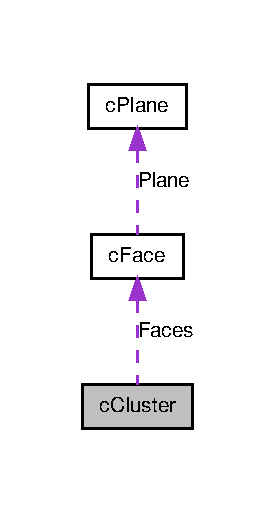
\includegraphics[width=134pt]{classc_cluster__coll__graph}
\end{center}
\end{figure}


\subsection{Detailed Description}
This class is an array of \hyperlink{classc_face}{cFace}. This is often used. 
\hypertarget{classc_collision_handler}{
\section{cCollisionHandler Class Reference}
\label{classc_collision_handler}\index{cCollisionHandler@{cCollisionHandler}}
}


This is the Collision Handler. It will control any collision search the user performs. This Collision handler is created by using the \hyperlink{classc_collision_handler_a04d5c8d5b7ac854b4958dca195bf1c1b}{Instance()} and can ONLY be created using \hyperlink{classc_collision_handler_a04d5c8d5b7ac854b4958dca195bf1c1b}{Instance()}. \_\-COLLISION\_\-HANDLER is a quick pointer to the \hyperlink{classc_collision_handler_a04d5c8d5b7ac854b4958dca195bf1c1b}{cCollisionHandler::Instance()} pointer. This will store data for the search and will store the current position to resume searches. Calling the Function GenerateCollisionList() wil create a comprehensive list of pointers to cRenderobjects() that meet the collision parameters of GenerateCollisionList(). This list can be accessed by using NextCollisionItem().  




Collaboration diagram for cCollisionHandler:\nopagebreak
\begin{figure}[H]
\begin{center}
\leavevmode
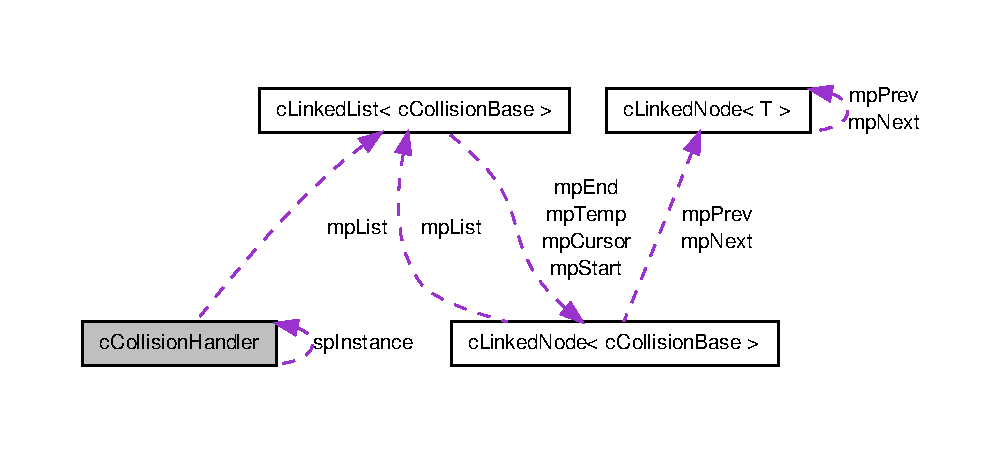
\includegraphics[width=400pt]{classc_collision_handler__coll__graph}
\end{center}
\end{figure}
\subsection*{Public Member Functions}
\begin{DoxyCompactItemize}
\item 
\hypertarget{classc_collision_handler_a5810098e3ca35eac5cb23936840787ef}{
virtual \hyperlink{classc_collision_handler_a5810098e3ca35eac5cb23936840787ef}{$\sim$cCollisionHandler} ()}
\label{classc_collision_handler_a5810098e3ca35eac5cb23936840787ef}

\begin{DoxyCompactList}\small\item\em This will deconstruct the class. \end{DoxyCompactList}\item 
\hypertarget{classc_collision_handler_a4fe00bffd2defe0a71a17c5fadd3b890}{
virtual void \hyperlink{classc_collision_handler_a4fe00bffd2defe0a71a17c5fadd3b890}{ResetCursors} ()=0}
\label{classc_collision_handler_a4fe00bffd2defe0a71a17c5fadd3b890}

\begin{DoxyCompactList}\small\item\em This will reset both the cursors used to track position through the collision object lists. \end{DoxyCompactList}\end{DoxyCompactItemize}
\subsection*{Static Public Member Functions}
\begin{DoxyCompactItemize}
\item 
\hypertarget{classc_collision_handler_a04d5c8d5b7ac854b4958dca195bf1c1b}{
static \hyperlink{classc_collision_handler}{cCollisionHandler} $\ast$ \hyperlink{classc_collision_handler_a04d5c8d5b7ac854b4958dca195bf1c1b}{Instance} ()}
\label{classc_collision_handler_a04d5c8d5b7ac854b4958dca195bf1c1b}

\begin{DoxyCompactList}\small\item\em This will return a pointer to the classes current instance and if there is none it will create one. \end{DoxyCompactList}\end{DoxyCompactItemize}
\subsection*{Protected Member Functions}
\begin{DoxyCompactItemize}
\item 
\hypertarget{classc_collision_handler_ae966359105ed5e144f62e36dd85d1f03}{
virtual \hyperlink{classc_linked_node}{cLinkedNode}$<$ \hyperlink{classc_collision_object}{cCollisionObject} $>$ $\ast$ \hyperlink{classc_collision_handler_ae966359105ed5e144f62e36dd85d1f03}{Add} (\hyperlink{classc_collision_object}{cCollisionObject} $\ast$lpTemp)=0}
\label{classc_collision_handler_ae966359105ed5e144f62e36dd85d1f03}

\begin{DoxyCompactList}\small\item\em This will add the \hyperlink{classc_collision_object}{cCollisionObject} pointed to by lpObject to the list mpList. \end{DoxyCompactList}\item 
\hypertarget{classc_collision_handler_aec2e30bb6be227d30daef0b6eb36d3b3}{
virtual void \hyperlink{classc_collision_handler_aec2e30bb6be227d30daef0b6eb36d3b3}{Remove} (\hyperlink{classc_linked_node}{cLinkedNode}$<$ \hyperlink{classc_collision_object}{cCollisionObject} $>$ $\ast$lpOld)}
\label{classc_collision_handler_aec2e30bb6be227d30daef0b6eb36d3b3}

\begin{DoxyCompactList}\small\item\em This will turn off Collisions for the \hyperlink{classc_linked_node}{cLinkedNode} lpOld. This should in turn call \hyperlink{classc_collision_handler_ad2d0933b78c692a5d2b3885242fa0911}{RemoveFromList()}. \end{DoxyCompactList}\item 
\hypertarget{classc_collision_handler_ad2d0933b78c692a5d2b3885242fa0911}{
virtual void \hyperlink{classc_collision_handler_ad2d0933b78c692a5d2b3885242fa0911}{RemoveFromList} (\hyperlink{classc_linked_node}{cLinkedNode}$<$ \hyperlink{classc_collision_object}{cCollisionObject} $>$ $\ast$lpOld)}
\label{classc_collision_handler_ad2d0933b78c692a5d2b3885242fa0911}

\begin{DoxyCompactList}\small\item\em This will acutally remove the clinkedNode from the relevant list. \end{DoxyCompactList}\item 
\hypertarget{classc_collision_handler_a906305fe520cefc195f3948458aba941}{
virtual bool \hyperlink{classc_collision_handler_a906305fe520cefc195f3948458aba941}{NextListItem} ()}
\label{classc_collision_handler_a906305fe520cefc195f3948458aba941}

\begin{DoxyCompactList}\small\item\em This will return the Next item in the lists in order. (The item is pointed to by mpColCur). If an item is found will return true, else will return false. \end{DoxyCompactList}\item 
\hypertarget{classc_collision_handler_a58b636db8343b7f4bbb27f3a93799e8b}{
virtual bool \hyperlink{classc_collision_handler_a58b636db8343b7f4bbb27f3a93799e8b}{NextListItem} (uint32 lpType)}
\label{classc_collision_handler_a58b636db8343b7f4bbb27f3a93799e8b}

\begin{DoxyCompactList}\small\item\em This will return the Next item in the list storing lpType in order. (the item is pointed to by mpColCur).If an item is found will return true, else will return false. \end{DoxyCompactList}\item 
\hypertarget{classc_collision_handler_ad2b079e234f956301fe83f5a5938cad0}{
virtual uint32 \hyperlink{classc_collision_handler_ad2b079e234f956301fe83f5a5938cad0}{FindSlot} (\hyperlink{classc_collision_object}{cCollisionObject} $\ast$lpObj)}
\label{classc_collision_handler_ad2b079e234f956301fe83f5a5938cad0}

\begin{DoxyCompactList}\small\item\em This will find the appropriate array slot for the \hyperlink{classc_collision_object}{cCollisionObject} lpObj. It will return the array position of the slot. \end{DoxyCompactList}\item 
\hypertarget{classc_collision_handler_aa6f7ca9d10b078ba11fcc3c0d266ab8e}{
virtual \hyperlink{classc_linked_list}{cLinkedList}$<$ \hyperlink{classc_collision_object}{cCollisionObject} $>$ $\ast$ \hyperlink{classc_collision_handler_aa6f7ca9d10b078ba11fcc3c0d266ab8e}{FindSlot} (uint32 $\ast$lpPos)}
\label{classc_collision_handler_aa6f7ca9d10b078ba11fcc3c0d266ab8e}

\begin{DoxyCompactList}\small\item\em This will return the list for the spatial slot lpPos\mbox{[}0\mbox{]},lpPos\mbox{[}1\mbox{]},lpPos\mbox{[}2\mbox{]}. (Array slots not spatial co-\/ordinates). \end{DoxyCompactList}\item 
\hypertarget{classc_collision_handler_aae512b7a5c7abb7307e7d25f22aa9fd0}{
virtual void \hyperlink{classc_collision_handler_aae512b7a5c7abb7307e7d25f22aa9fd0}{Position} (float $\ast$lpTemp)}
\label{classc_collision_handler_aae512b7a5c7abb7307e7d25f22aa9fd0}

\begin{DoxyCompactList}\small\item\em This will set the current Position of the Spatial Array. \end{DoxyCompactList}\item 
\hypertarget{classc_collision_handler_af02385e0c91e4c73c521e65477efed2c}{
virtual float $\ast$ \hyperlink{classc_collision_handler_af02385e0c91e4c73c521e65477efed2c}{Position} ()}
\label{classc_collision_handler_af02385e0c91e4c73c521e65477efed2c}

\begin{DoxyCompactList}\small\item\em This will return the current Position of the Spatial Array. \end{DoxyCompactList}\end{DoxyCompactItemize}
\subsection*{Protected Attributes}
\begin{DoxyCompactItemize}
\item 
\hypertarget{classc_collision_handler_a959870d5beee77a014b29e45bf153723}{
\hyperlink{classc_linked_list}{cLinkedList}$<$ \hyperlink{classc_collision_object}{cCollisionObject} $>$ $\ast$ \hyperlink{classc_collision_handler_a959870d5beee77a014b29e45bf153723}{mpList}}
\label{classc_collision_handler_a959870d5beee77a014b29e45bf153723}

\begin{DoxyCompactList}\small\item\em This is an array for storing all Collision Objects, that are currently on. The size of the array is set by WT\_\-COLLISION\_\-HANDLER\_\-ARRAY\_\-SIZE. \end{DoxyCompactList}\end{DoxyCompactItemize}
\subsection*{Static Protected Attributes}
\begin{DoxyCompactItemize}
\item 
\hypertarget{classc_collision_handler_ae020327c284763548d259a3d35a8f537}{
static \hyperlink{classc_collision_handler}{cCollisionHandler} $\ast$ \hyperlink{classc_collision_handler_ae020327c284763548d259a3d35a8f537}{spInstance}}
\label{classc_collision_handler_ae020327c284763548d259a3d35a8f537}

\begin{DoxyCompactList}\small\item\em This is a pointer to the classes current instance. There can only be one... \end{DoxyCompactList}\end{DoxyCompactItemize}
\subsection*{Friends}
\begin{DoxyCompactItemize}
\item 
\hypertarget{classc_collision_handler_a3fc30c810c62135f498c47205c853e30}{
class \hyperlink{classc_collision_handler_a3fc30c810c62135f498c47205c853e30}{cCollisionObject}}
\label{classc_collision_handler_a3fc30c810c62135f498c47205c853e30}

\end{DoxyCompactItemize}


\subsection{Detailed Description}
This is the Collision Handler. It will control any collision search the user performs. This Collision handler is created by using the \hyperlink{classc_collision_handler_a04d5c8d5b7ac854b4958dca195bf1c1b}{Instance()} and can ONLY be created using \hyperlink{classc_collision_handler_a04d5c8d5b7ac854b4958dca195bf1c1b}{Instance()}. \_\-COLLISION\_\-HANDLER is a quick pointer to the \hyperlink{classc_collision_handler_a04d5c8d5b7ac854b4958dca195bf1c1b}{cCollisionHandler::Instance()} pointer. This will store data for the search and will store the current position to resume searches. Calling the Function GenerateCollisionList() wil create a comprehensive list of pointers to cRenderobjects() that meet the collision parameters of GenerateCollisionList(). This list can be accessed by using NextCollisionItem(). 

The sizes and positions of objects are calculated during a render cycle. ????Objects will not collide until after their first render cycle.

There are three types of Collision Searches. Tree, Type and Binary Spatial Position. (defined by setting WT\_\-COLLISION\_\-HANDLER\_\-TYPE to WT\_\-COLLISION\_\-HANDLER\_\-TYPE\_\-TYPE or WT\_\-COLLISION\_\-HANDLER\_\-TYPE\_\-BSP.

Tree searches are performed by traversing the render tree. Each objects size is based on the size of the objects beneath it so if a Node does not collide all objects beneath that node can be ignored.

Type searches are filtered by type. cCollisionObject's are given a \hyperlink{classc_collision_object_a2a527f445a899adafbf18dddf140e179}{cCollisionObject::CollisionFilter(uint32 liID)} using which they are sorted into seperate lists of Collision objects. If a search is performed with a defined ID term, only the list containing objects with the desired filter value are searched.

Binary Spatial Position Collision Handlers sort cCollisionObjects into the spatial boxes they contact with. This means it is only neccessary to check other objects within the boxes the current object resides within. 
\hypertarget{classc_collision_list}{
\section{cCollisionList Class Reference}
\label{classc_collision_list}\index{cCollisionList@{cCollisionList}}
}


This is generated by doing Collision Detection with an object. This will cache all the detected collisions with the object used for the collision detection. This allows the user to access the collisions in a different order to the order they were detected or to cache it for use later. The list is composed of a list of \hyperlink{classc_collision_list_object}{cCollisionListObject}.  




Collaboration diagram for cCollisionList:\nopagebreak
\begin{figure}[H]
\begin{center}
\leavevmode
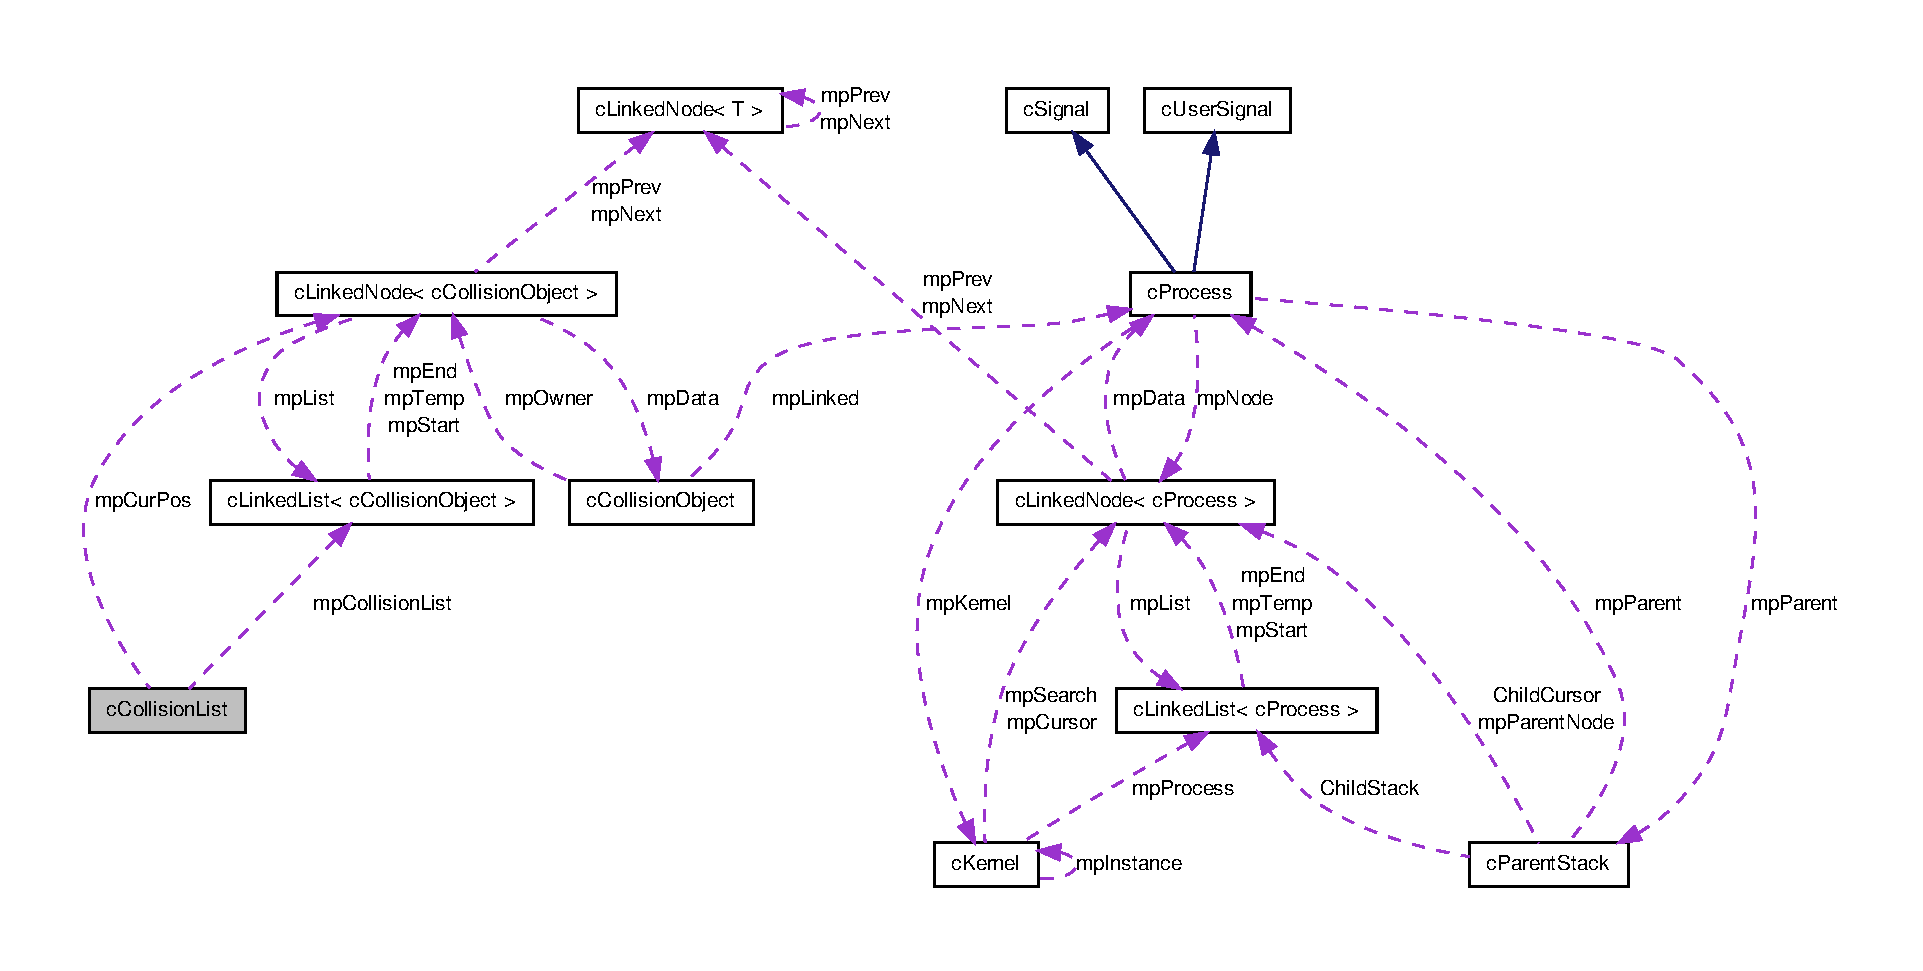
\includegraphics[width=400pt]{classc_collision_list__coll__graph}
\end{center}
\end{figure}
\subsection*{Public Member Functions}
\begin{DoxyCompactItemize}
\item 
\hypertarget{classc_collision_list_a1b84b682ec105262682532b0a90754c2}{
\hyperlink{classc_collision_list_a1b84b682ec105262682532b0a90754c2}{cCollisionList} ()}
\label{classc_collision_list_a1b84b682ec105262682532b0a90754c2}

\begin{DoxyCompactList}\small\item\em The Constructor for \hyperlink{classc_collision_list}{cCollisionList}. \end{DoxyCompactList}\item 
\hypertarget{classc_collision_list_ace525d10fc1a38477cee11e14714b476}{
void \hyperlink{classc_collision_list_ace525d10fc1a38477cee11e14714b476}{AddCollision} (\hyperlink{classc_collision_object}{cCollisionObject} $\ast$lpObject)}
\label{classc_collision_list_ace525d10fc1a38477cee11e14714b476}

\begin{DoxyCompactList}\small\item\em This will Add the object lpObject to the list of objects colliding with the current searching object. \end{DoxyCompactList}\item 
\hypertarget{classc_collision_list_adeef80e9e181e81dc073ebcfa1d8bec4}{
\hyperlink{classc_collision_object}{cCollisionObject} $\ast$ \hyperlink{classc_collision_list_adeef80e9e181e81dc073ebcfa1d8bec4}{NextCollisionItem} ()}
\label{classc_collision_list_adeef80e9e181e81dc073ebcfa1d8bec4}

\begin{DoxyCompactList}\small\item\em This will return the next item from the list mpCollisionList that has been stocked by GenerateCollisionList() as a CollisionObject pointer. \end{DoxyCompactList}\item 
\hypertarget{classc_collision_list_ac641346bbc7e3d3b84880ae03b0496c5}{
\hyperlink{classc_process}{cProcess} $\ast$ \hyperlink{classc_collision_list_ac641346bbc7e3d3b84880ae03b0496c5}{NextCollisionP} ()}
\label{classc_collision_list_ac641346bbc7e3d3b84880ae03b0496c5}

\begin{DoxyCompactList}\small\item\em This will return the process owning renderable object creating the next detected collision. \end{DoxyCompactList}\item 
\hypertarget{classc_collision_list_a87c8ee3baa85ff002030c83bd1784192}{
vRenderObject $\ast$ \hyperlink{classc_collision_list_a87c8ee3baa85ff002030c83bd1784192}{NextCollisionR} ()}
\label{classc_collision_list_a87c8ee3baa85ff002030c83bd1784192}

\begin{DoxyCompactList}\small\item\em This will return the renderable object involved in the next detected collision. \end{DoxyCompactList}\item 
\hypertarget{classc_collision_list_ac04316a4e8d0e3c5c3213c20bd7897cc}{
void \hyperlink{classc_collision_list_ac04316a4e8d0e3c5c3213c20bd7897cc}{ResetList} ()}
\label{classc_collision_list_ac04316a4e8d0e3c5c3213c20bd7897cc}

\begin{DoxyCompactList}\small\item\em This will reset the collision search to the start of mpList. \end{DoxyCompactList}\item 
\hypertarget{classc_collision_list_a628ed6510cd89c192a402be0a64ea111}{
\hyperlink{classc_collision_list_a628ed6510cd89c192a402be0a64ea111}{$\sim$cCollisionList} ()}
\label{classc_collision_list_a628ed6510cd89c192a402be0a64ea111}

\begin{DoxyCompactList}\small\item\em This is the destructor for \hyperlink{classc_collision_list}{cCollisionList}. \end{DoxyCompactList}\item 
\hypertarget{classc_collision_list_ae279c0239ead11e2d6c3647495347cc4}{
void \hyperlink{classc_collision_list_ae279c0239ead11e2d6c3647495347cc4}{SortByDistance} ()}
\label{classc_collision_list_ae279c0239ead11e2d6c3647495347cc4}

\begin{DoxyCompactList}\small\item\em This will sort the list of collisionobjects into distance from the colliding object order. This allows the user to resolve the collisions in 'Chronological' order. \end{DoxyCompactList}\end{DoxyCompactItemize}


\subsection{Detailed Description}
This is generated by doing Collision Detection with an object. This will cache all the detected collisions with the object used for the collision detection. This allows the user to access the collisions in a different order to the order they were detected or to cache it for use later. The list is composed of a list of \hyperlink{classc_collision_list_object}{cCollisionListObject}. 
\hypertarget{classc_collision_list_object}{
\section{cCollisionListObject Class Reference}
\label{classc_collision_list_object}\index{cCollisionListObject@{cCollisionListObject}}
}


Collaboration diagram for cCollisionListObject:
\nopagebreak
\begin{figure}[H]
\begin{center}
\leavevmode
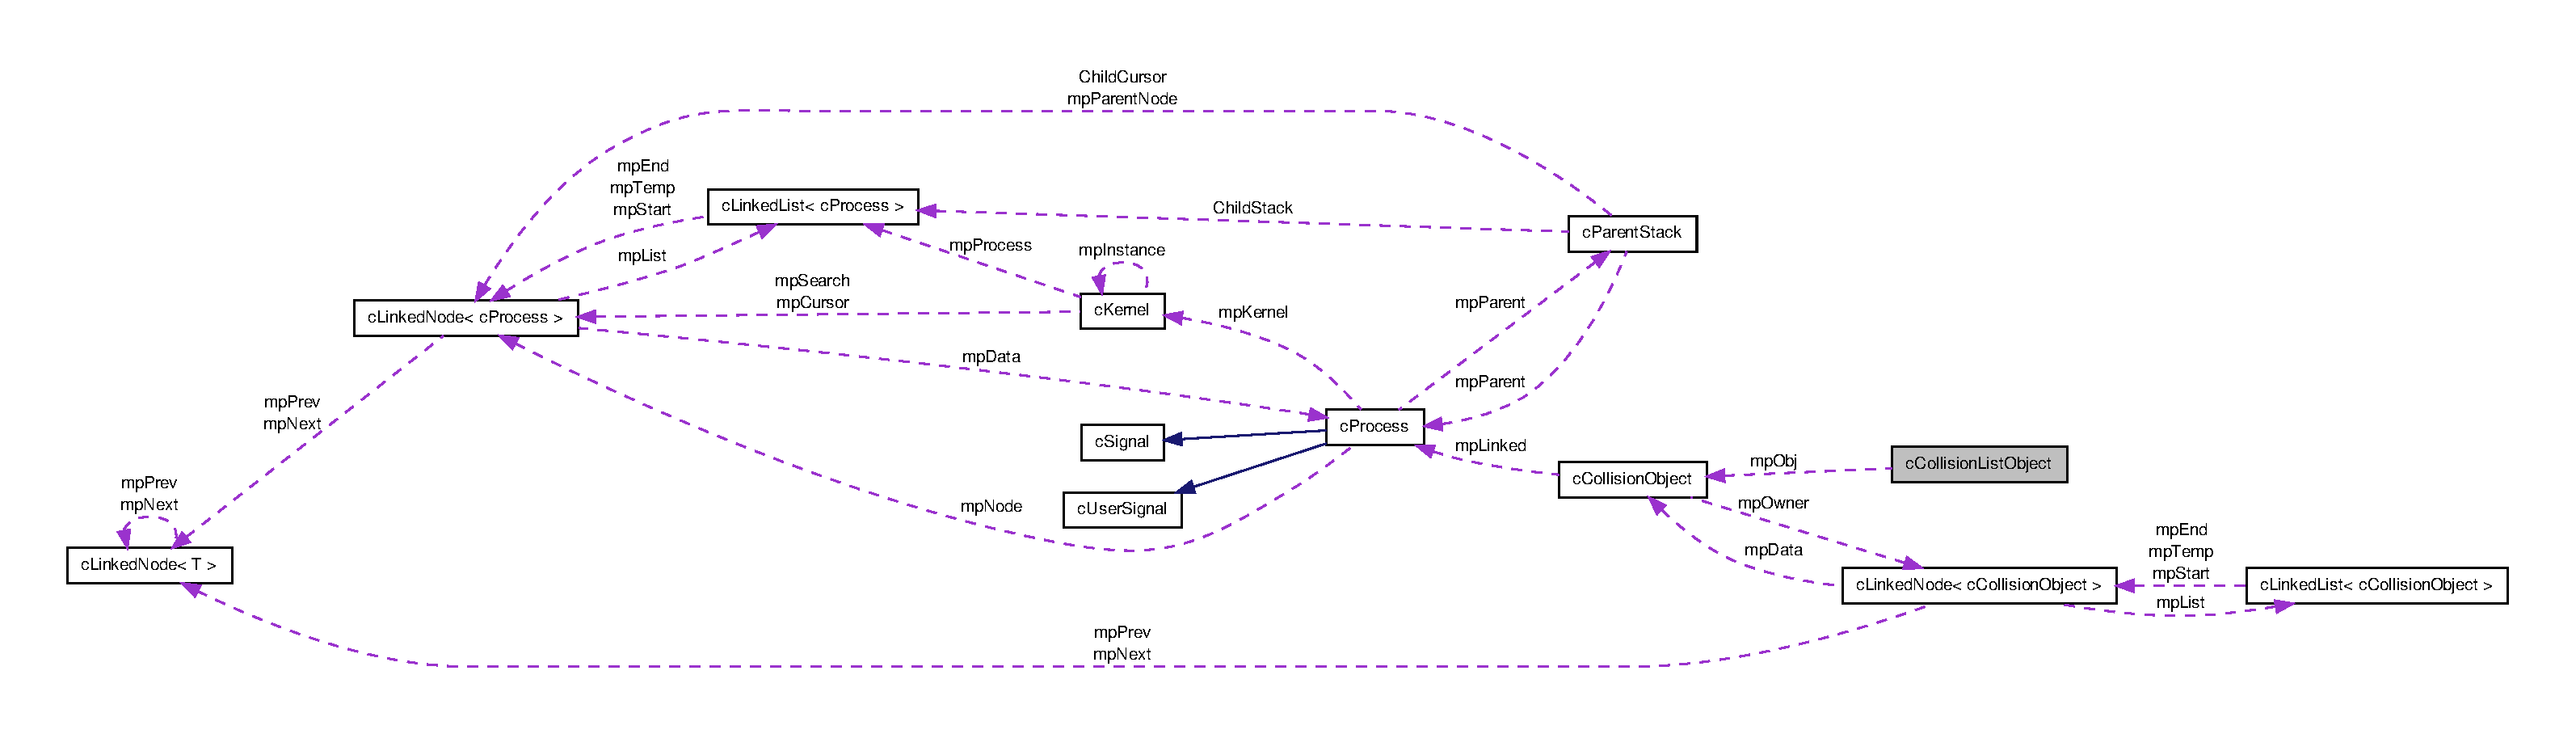
\includegraphics[width=400pt]{classc_collision_list_object__coll__graph}
\end{center}
\end{figure}
\subsection*{Public Member Functions}
\begin{DoxyCompactItemize}
\item 
\hyperlink{classc_collision_list_object_a08d25f1e82853098b07ad9c30c8b21a8}{cCollisionListObject} (\hyperlink{classc_collision_object}{cCollisionObject} $\ast$lpObj)
\item 
float \hyperlink{classc_collision_list_object_a1f78164f5389c06744a447c9caf86372}{GetDistance} ()
\end{DoxyCompactItemize}


\subsection{Detailed Description}


Definition at line 4 of file WTcCollisionList.h.



\subsection{Constructor \& Destructor Documentation}
\hypertarget{classc_collision_list_object_a08d25f1e82853098b07ad9c30c8b21a8}{
\index{cCollisionListObject@{cCollisionListObject}!cCollisionListObject@{cCollisionListObject}}
\index{cCollisionListObject@{cCollisionListObject}!cCollisionListObject@{cCollisionListObject}}
\subsubsection[{cCollisionListObject}]{\setlength{\rightskip}{0pt plus 5cm}cCollisionListObject::cCollisionListObject (
\begin{DoxyParamCaption}
\item[{{\bf cCollisionObject} $\ast$}]{lpObj}
\end{DoxyParamCaption}
)\hspace{0.3cm}{\ttfamily  \mbox{[}inline\mbox{]}}}}
\label{classc_collision_list_object_a08d25f1e82853098b07ad9c30c8b21a8}


Definition at line 9 of file WTcCollisionList.h.



\subsection{Member Function Documentation}
\hypertarget{classc_collision_list_object_a1f78164f5389c06744a447c9caf86372}{
\index{cCollisionListObject@{cCollisionListObject}!GetDistance@{GetDistance}}
\index{GetDistance@{GetDistance}!cCollisionListObject@{cCollisionListObject}}
\subsubsection[{GetDistance}]{\setlength{\rightskip}{0pt plus 5cm}float cCollisionListObject::GetDistance (
\begin{DoxyParamCaption}
{}
\end{DoxyParamCaption}
)\hspace{0.3cm}{\ttfamily  \mbox{[}inline\mbox{]}}}}
\label{classc_collision_list_object_a1f78164f5389c06744a447c9caf86372}


Definition at line 10 of file WTcCollisionList.h.


\hypertarget{classc_collision_object}{
\section{cCollisionObject Class Reference}
\label{classc_collision_object}\index{cCollisionObject@{cCollisionObject}}
}


Inheritance diagram for cCollisionObject:
\nopagebreak
\begin{figure}[H]
\begin{center}
\leavevmode
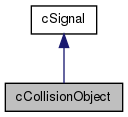
\includegraphics[width=168pt]{classc_collision_object__inherit__graph}
\end{center}
\end{figure}


Collaboration diagram for cCollisionObject:
\nopagebreak
\begin{figure}[H]
\begin{center}
\leavevmode
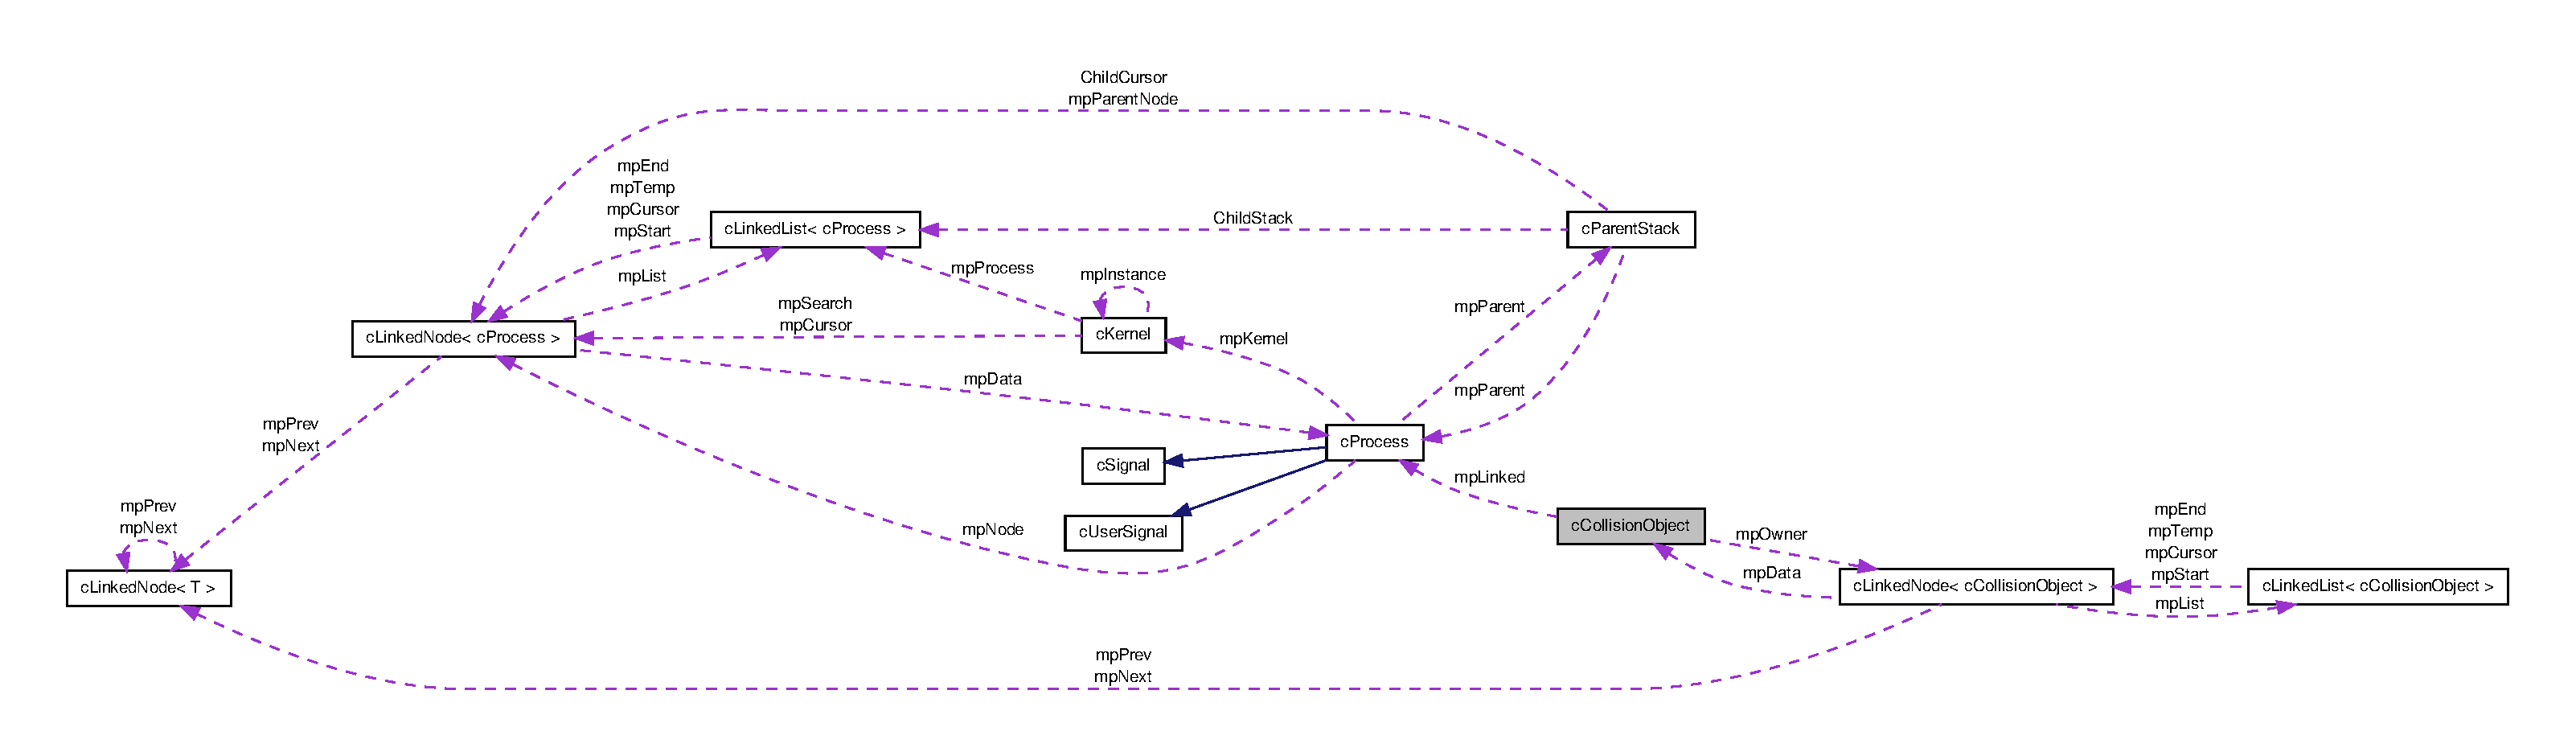
\includegraphics[width=400pt]{classc_collision_object__coll__graph}
\end{center}
\end{figure}
\subsection*{Public Member Functions}
\begin{DoxyCompactItemize}
\item 
\hyperlink{classc_collision_object_a90f4a7fe0445396ddf49e14bda27f2dc}{cCollisionObject} (\hyperlink{classv_render_object}{vRenderObject} $\ast$lpFollow, \hyperlink{classv_process}{vProcess} $\ast$lpLinked=0, uint32 liFilterType=0)
\item 
\hyperlink{classc_collision_object_a38fc1abcd7a0f240d7ce41aca108bb43}{cCollisionObject} (\hyperlink{classc_beam_mesh}{cBeamMesh} $\ast$lpFollow, \hyperlink{classv_process}{vProcess} $\ast$lpLinked=0, uint32 liFilterType=0)
\item 
void \hyperlink{classc_collision_object_a4aaae58a85bd7c1e6b5601a4e4cac3c1}{Initialise} (\hyperlink{classv_render_object}{vRenderObject} $\ast$lpFollow, \hyperlink{classv_process}{vProcess} $\ast$lpLinked, uint32 liFilterType)
\item 
\hyperlink{classc_collision_object_ac01e53c6dadd3ab8036f485b9115aedd}{$\sim$cCollisionObject} ()
\item 
bool \hyperlink{classc_collision_object_ac56988f3641d39409fbf4ccba3525282}{CreatedThisFrame} ()
\item 
void \hyperlink{classc_collision_object_a31156a5bfff63de45daa32893a30697c}{NotCreatedThisFrame} ()
\item 
\hyperlink{classv_collision_data}{vCollisionData} $\ast$ \hyperlink{classc_collision_object_a58a3680126c2d7e405ec80402cb8208e}{CollisionData} ()
\item 
void \hyperlink{classc_collision_object_abec1a68ab54f2e80244c8b336bca3626}{Signal} (SIGNAL liFlags)
\begin{DoxyCompactList}\small\item\em This is the function that will handle a system signal. Possible signals to be passed in are \_\-S\_\-SLEEP,\_\-S\_\-WAKE,\_\-S\_\-KILL,\_\-S\_\-SLEEP\_\-TREE, \_\-S\_\-WAKE\_\-TREE,\_\-S\_\-KILL\_\-TREE. \item\end{DoxyCompactList}\item 
bool \hyperlink{classc_collision_object_a9d4e4fe61df1af3479247611d605e897}{Procedural} ()
\item 
bool \hyperlink{classc_collision_object_a695516ede632cf0e02ddbcd7b6e539a7}{Loaded} ()
\item 
void \hyperlink{classc_collision_object_a908a1cbe39b07c53849f60fecb5230dc}{ClearProcedural} ()
\item 
\hyperlink{classc_sphere_collision}{cSphereCollision} $\ast$ \hyperlink{classc_collision_object_afe43e12c0ea0da5c3653450cb8dfb047}{Sphere} ()
\item 
\hyperlink{classc_mesh_collision}{cMeshCollision} $\ast$ \hyperlink{classc_collision_object_a6ea07e3f2501b7092fed0130f150c4f4}{Mesh} ()
\item 
\hyperlink{classc_ray_collision}{cRayCollision} $\ast$ \hyperlink{classc_collision_object_ac46982867551f6dd05c0dbcae0e57796}{Ray} ()
\item 
\hyperlink{classc_beam_collision}{cBeamCollision} $\ast$ \hyperlink{classc_collision_object_a8a5a6900686ac3ac88cf6bdac71569ad}{Beam} ()
\item 
void \hyperlink{classc_collision_object_ae465362052ff2026ed31c2fa3664d209}{SetType} (\hyperlink{classc_sphere_collision}{cSphereCollision} $\ast$lpSphere)
\begin{DoxyCompactList}\small\item\em This will take a SphereCollision Object loaded from a file, and set this Collision Object to use it. \item\end{DoxyCompactList}\item 
void \hyperlink{classc_collision_object_a5c46dea7134fa466293938c22a780529}{SetType} (\hyperlink{classc_mesh_collision}{cMeshCollision} $\ast$lpMesh)
\begin{DoxyCompactList}\small\item\em This will take a MeshCollision Object loaded from a file, and set this Collision Object to use it. \item\end{DoxyCompactList}\item 
void \hyperlink{classc_collision_object_a4282627cb1818f66842f3c8ff91cd20e}{SetType} (\hyperlink{classc_beam_collision}{cBeamCollision} $\ast$lpBeam)
\begin{DoxyCompactList}\small\item\em This will take a BeamCollision Object loaded from a file, and set this Collision Object to use it. \item\end{DoxyCompactList}\item 
void \hyperlink{classc_collision_object_a8ef73a19857e4a35470502776b0f03f8}{OnFile} (\hyperlink{classv_collision_data}{vCollisionData} $\ast$lpPoint)
\item 
void \hyperlink{classc_collision_object_a6ea3e10f69f7a2d5cae2bd4471461137}{OnProcedural} ()
\item 
\hyperlink{classc_sphere_collision}{cSphereCollision} $\ast$ \hyperlink{classc_collision_object_a22e6f4f5c722b6d45629d92488e5d925}{SetType} (float lfSize)
\begin{DoxyCompactList}\small\item\em This will procedurally generate a Sphere or radius 1.0f;. \item\end{DoxyCompactList}\item 
\hyperlink{classc_beam_collision}{cBeamCollision} $\ast$ \hyperlink{classc_collision_object_ab5fc1f36d50ea87a69b4879076a92533}{SetType} (float lfLength, float lfRadius)
\begin{DoxyCompactList}\small\item\em This will procedurally generate a Beam of Radius lfRadius and Length lfLength. \item\end{DoxyCompactList}\item 
\hyperlink{classc_mesh_collision}{cMeshCollision} $\ast$ \hyperlink{classc_collision_object_a40b80411356222997bb94fae10796c93}{SetType} (float $\ast$lpBounds)
\begin{DoxyCompactList}\small\item\em This will procedureally generate a Box collision object from the array of 6 floats lpBounds. see cGeneratedBoxCollision::BuildObject(float $\ast$lpBounds) for more information. \item\end{DoxyCompactList}\item 
\hyperlink{classc_ray_collision}{cRayCollision} $\ast$ \hyperlink{classc_collision_object_a761dae3de0ea58d4d60b98348177b7ed}{SetType} (\hyperlink{classc_render_object}{cRenderObject} $\ast$lpObj)
\begin{DoxyCompactList}\small\item\em This will make a ray object. See cRayCollision::BuildObject(float $\ast$lpBounds) for more information. Makes Ray radius to be same as object and ray to follow it's movement. \item\end{DoxyCompactList}\item 
\hyperlink{classc_beam_collision}{cBeamCollision} $\ast$ \hyperlink{classc_collision_object_a0d08a63b8b7a3bcf6eb1c6617ec71e91}{SetType} (\hyperlink{classc_beam_mesh}{cBeamMesh} $\ast$lpBeam)
\begin{DoxyCompactList}\small\item\em This will make a Beam object to match a rendered Beam. (Nice and easy eh?) \item\end{DoxyCompactList}\item 
\hyperlink{classc_sphere_collision}{cSphereCollision} $\ast$ \hyperlink{classc_collision_object_add80d08291b6c162bdf9b5f7408d6617}{GetCollisionData} ()
\item 
uint8 \hyperlink{classc_collision_object_ae1274b9a69dfa081cda23a840c9e2df4}{Type} ()
\begin{DoxyCompactList}\small\item\em This is the accurate way of determining the type of these objects. \item\end{DoxyCompactList}\item 
bool \hyperlink{classc_collision_object_a6f5b5341a726cb0a54fe3271b110dc8c}{CheckCollision} (\hyperlink{classc_collision_object}{cCollisionObject} $\ast$lpOther)
\begin{DoxyCompactList}\small\item\em This will check for a collision between this object and the object lpOther. \item\end{DoxyCompactList}\item 
bool \hyperlink{classc_collision_object_a1d93858e03da25f8656ae688c4dedbce}{TouchCollision} (\hyperlink{classc_collision_object}{cCollisionObject} $\ast$lpOther)
\item 
\hyperlink{classc_matrix4}{cMatrix4} \& \hyperlink{classc_collision_object_abc47ab584910cc877b5e723be4e09eac}{CacheMatrix} ()
\begin{DoxyCompactList}\small\item\em This will return the Objects Cached Matrix mmCache. \item\end{DoxyCompactList}\item 
\hyperlink{classv_render_object}{vRenderObject} $\ast$ \hyperlink{classc_collision_object_a959994c60b68de6be85dcc663228bab8}{RenderObject} ()
\begin{DoxyCompactList}\small\item\em This will return a pointer the \hyperlink{classc_render_object}{cRenderObject} linked to this. \item\end{DoxyCompactList}\item 
uint32 \hyperlink{classc_collision_object_a1490cdf75c8037049bfa7891aa8756b7}{CollisionFilter} ()
\begin{DoxyCompactList}\small\item\em This will return the current Collision Filter ID of this object. \item\end{DoxyCompactList}\item 
void \hyperlink{classc_collision_object_a2a527f445a899adafbf18dddf140e179}{CollisionFilter} (uint32 liID)
\begin{DoxyCompactList}\small\item\em This will set the Collision Filter ID of this object. \item\end{DoxyCompactList}\item 
bool \hyperlink{classc_collision_object_ae9f62c64221d8cc347010fed3cf6e8d1}{Collision} (\hyperlink{classc_collision_object}{cCollisionObject} $\ast$lpOther, uint32 lpCol)
\item 
bool \hyperlink{classc_collision_object_abf62376a5806d878b5810acfd40bc450}{Collision} (\hyperlink{classc_collision_object}{cCollisionObject} $\ast$lpOther)
\item 
bool \hyperlink{classc_collision_object_acc8e58a747eba8e5c7903c8d769b9b31}{CompareRanges} (float lf1, float lf2, float lfR)
\begin{DoxyCompactList}\small\item\em This will do a sphere collision between two points. lf1 and lf2 are x$\ast$x+y$\ast$y+z$\ast$z. lfR is (Sum of Radii)$\ast$(Sum of Radii). \item\end{DoxyCompactList}\item 
void \hyperlink{classc_collision_object_a30475084c3b15f9bf8dc8818ed486c7d}{SetLink} (\hyperlink{classv_process}{vProcess} $\ast$lpLink)
\begin{DoxyCompactList}\small\item\em This sets the process that this renderable object will return collision signals to. \item\end{DoxyCompactList}\item 
\hyperlink{classv_process}{vProcess} $\ast$ \hyperlink{classc_collision_object_a7b501c8848f32131eb36b1f7f69c21ec}{GetLink} ()
\begin{DoxyCompactList}\small\item\em Returns the process currently linked to this renderable object. \item\end{DoxyCompactList}\item 
void \hyperlink{classc_collision_object_a40afa697b7e09e716b471725e6e33805}{GenerateCollisionList} (uint32 liType=0)
\begin{DoxyCompactList}\small\item\em This will generate a collision list of all objects colliding with this object filtered by type liType. \item\end{DoxyCompactList}\item 
float $\ast$ \hyperlink{classc_collision_object_a66f5ab6f3e5b3d618625b8c254f477ab}{GetPos} ()
\begin{DoxyCompactList}\small\item\em This will return the position of the selected object. \item\end{DoxyCompactList}\item 
void \hyperlink{classc_collision_object_a86932ba04099dd34874fd3ada314168c}{PreUpdateCache} ()
\begin{DoxyCompactList}\small\item\em This will remove the \hyperlink{classc_collision_object}{cCollisionObject} from it's Spatial Slots before its position is updated. \item\end{DoxyCompactList}\item 
void \hyperlink{classc_collision_object_a7719840f3fcc5bf3dcef08d123066739}{PostUpdateCache} ()
\begin{DoxyCompactList}\small\item\em This will Add the \hyperlink{classc_collision_object}{cCollisionObject} to the relevant Spatial Slots after it has found it's new position. \item\end{DoxyCompactList}\item 
bool \hyperlink{classc_collision_object_a53623f53b0ac497bfa1c794a76d2f818}{SphereSphere} (\hyperlink{classc_collision_object}{cCollisionObject} $\ast$lpOther)
\item 
bool \hyperlink{classc_collision_object_ae87264d7ecd143a67244c95b10c07ab7}{ModelModel} (\hyperlink{classc_collision_object}{cCollisionObject} $\ast$lpOther)
\item 
bool \hyperlink{classc_collision_object_aa4500b5834736e5abeabe71c300e64e8}{RayRay} (\hyperlink{classc_collision_object}{cCollisionObject} $\ast$lpOther)
\item 
bool \hyperlink{classc_collision_object_a299e49b5d78e1e7dbe5e801c7760462a}{SphereModel} (\hyperlink{classc_collision_object}{cCollisionObject} $\ast$lpOther)
\item 
bool \hyperlink{classc_collision_object_ae4761ec4a0f60667e83cb6d4cf39d359}{SphereRay} (\hyperlink{classc_collision_object}{cCollisionObject} $\ast$lpOther)
\item 
bool \hyperlink{classc_collision_object_a7ccea939e1f91fa7eeda4c31128901c3}{RayModel} (\hyperlink{classc_collision_object}{cCollisionObject} $\ast$lpOther)
\item 
float \hyperlink{classc_collision_object_ae6c320e7a3361fbbc4796463d777daab}{GetCollisionSize} ()
\end{DoxyCompactItemize}
\subsection*{Static Public Attributes}
\begin{DoxyCompactItemize}
\item 
static float \hyperlink{classc_collision_object_a3afac28cfda77f7ed63605e604c1139a}{mfStaticSize} \mbox{[}3\mbox{]} = \{0.0f,0.0f,0.0f\}
\begin{DoxyCompactList}\small\item\em This is a temporary storage for transfering sizes between objects. \item\end{DoxyCompactList}\end{DoxyCompactItemize}


\subsection{Detailed Description}


Definition at line 14 of file WTcCollisionObject.h.



\subsection{Constructor \& Destructor Documentation}
\hypertarget{classc_collision_object_a90f4a7fe0445396ddf49e14bda27f2dc}{
\index{cCollisionObject@{cCollisionObject}!cCollisionObject@{cCollisionObject}}
\index{cCollisionObject@{cCollisionObject}!cCollisionObject@{cCollisionObject}}
\subsubsection[{cCollisionObject}]{\setlength{\rightskip}{0pt plus 5cm}cCollisionObject::cCollisionObject (
\begin{DoxyParamCaption}
\item[{{\bf vRenderObject} $\ast$}]{lpFollow, }
\item[{{\bf vProcess} $\ast$}]{lpLinked = {\ttfamily 0}, }
\item[{uint32}]{liFilterType = {\ttfamily 0}}
\end{DoxyParamCaption}
)}}
\label{classc_collision_object_a90f4a7fe0445396ddf49e14bda27f2dc}


Definition at line 839 of file WTcCollisionObject.cpp.

\hypertarget{classc_collision_object_a38fc1abcd7a0f240d7ce41aca108bb43}{
\index{cCollisionObject@{cCollisionObject}!cCollisionObject@{cCollisionObject}}
\index{cCollisionObject@{cCollisionObject}!cCollisionObject@{cCollisionObject}}
\subsubsection[{cCollisionObject}]{\setlength{\rightskip}{0pt plus 5cm}cCollisionObject::cCollisionObject (
\begin{DoxyParamCaption}
\item[{{\bf cBeamMesh} $\ast$}]{lpFollow, }
\item[{{\bf vProcess} $\ast$}]{lpLinked = {\ttfamily 0}, }
\item[{uint32}]{liFilterType = {\ttfamily 0}}
\end{DoxyParamCaption}
)}}
\label{classc_collision_object_a38fc1abcd7a0f240d7ce41aca108bb43}


Definition at line 856 of file WTcCollisionObject.cpp.

\hypertarget{classc_collision_object_ac01e53c6dadd3ab8036f485b9115aedd}{
\index{cCollisionObject@{cCollisionObject}!$\sim$cCollisionObject@{$\sim$cCollisionObject}}
\index{$\sim$cCollisionObject@{$\sim$cCollisionObject}!cCollisionObject@{cCollisionObject}}
\subsubsection[{$\sim$cCollisionObject}]{\setlength{\rightskip}{0pt plus 5cm}cCollisionObject::$\sim$cCollisionObject (
\begin{DoxyParamCaption}
{}
\end{DoxyParamCaption}
)}}
\label{classc_collision_object_ac01e53c6dadd3ab8036f485b9115aedd}


Definition at line 754 of file WTcCollisionObject.cpp.



\subsection{Member Function Documentation}
\hypertarget{classc_collision_object_a8a5a6900686ac3ac88cf6bdac71569ad}{
\index{cCollisionObject@{cCollisionObject}!Beam@{Beam}}
\index{Beam@{Beam}!cCollisionObject@{cCollisionObject}}
\subsubsection[{Beam}]{\setlength{\rightskip}{0pt plus 5cm}{\bf cBeamCollision}$\ast$ cCollisionObject::Beam (
\begin{DoxyParamCaption}
{}
\end{DoxyParamCaption}
)\hspace{0.3cm}{\ttfamily  \mbox{[}inline\mbox{]}}}}
\label{classc_collision_object_a8a5a6900686ac3ac88cf6bdac71569ad}
This is a dynamic cast on the type of collision object this is. Note ALL cCollisionData objects return true to Sphere. This applies to all the functions \hyperlink{classc_collision_object_afe43e12c0ea0da5c3653450cb8dfb047}{Sphere()},Box(),\hyperlink{classc_collision_object_a6ea07e3f2501b7092fed0130f150c4f4}{Mesh()},\hyperlink{classc_collision_object_ac46982867551f6dd05c0dbcae0e57796}{Ray()} and \hyperlink{classc_collision_object_a8a5a6900686ac3ac88cf6bdac71569ad}{Beam()}. 

Definition at line 74 of file WTcCollisionObject.h.

\hypertarget{classc_collision_object_abc47ab584910cc877b5e723be4e09eac}{
\index{cCollisionObject@{cCollisionObject}!CacheMatrix@{CacheMatrix}}
\index{CacheMatrix@{CacheMatrix}!cCollisionObject@{cCollisionObject}}
\subsubsection[{CacheMatrix}]{\setlength{\rightskip}{0pt plus 5cm}{\bf cMatrix4}\& cCollisionObject::CacheMatrix (
\begin{DoxyParamCaption}
{}
\end{DoxyParamCaption}
)\hspace{0.3cm}{\ttfamily  \mbox{[}inline\mbox{]}}}}
\label{classc_collision_object_abc47ab584910cc877b5e723be4e09eac}


This will return the Objects Cached Matrix mmCache. 



Definition at line 142 of file WTcCollisionObject.h.

\hypertarget{classc_collision_object_a6f5b5341a726cb0a54fe3271b110dc8c}{
\index{cCollisionObject@{cCollisionObject}!CheckCollision@{CheckCollision}}
\index{CheckCollision@{CheckCollision}!cCollisionObject@{cCollisionObject}}
\subsubsection[{CheckCollision}]{\setlength{\rightskip}{0pt plus 5cm}bool cCollisionObject::CheckCollision (
\begin{DoxyParamCaption}
\item[{{\bf cCollisionObject} $\ast$}]{lpOther}
\end{DoxyParamCaption}
)}}
\label{classc_collision_object_a6f5b5341a726cb0a54fe3271b110dc8c}


This will check for a collision between this object and the object lpOther. 

$\ast$ 
\begin{DoxyParams}{Parameters}
{\em lpOther} & is a pointer to the other collision object to check against. It will check both objects have collisions on. Then it will do an initial quick check to see if a collision is a possibility. Finally if required it will do a much more detailed collision check. \\
\hline
\end{DoxyParams}


Definition at line 673 of file WTcCollisionObject.cpp.

\hypertarget{classc_collision_object_a908a1cbe39b07c53849f60fecb5230dc}{
\index{cCollisionObject@{cCollisionObject}!ClearProcedural@{ClearProcedural}}
\index{ClearProcedural@{ClearProcedural}!cCollisionObject@{cCollisionObject}}
\subsubsection[{ClearProcedural}]{\setlength{\rightskip}{0pt plus 5cm}void cCollisionObject::ClearProcedural (
\begin{DoxyParamCaption}
{}
\end{DoxyParamCaption}
)}}
\label{classc_collision_object_a908a1cbe39b07c53849f60fecb5230dc}


Definition at line 871 of file WTcCollisionObject.cpp.

\hypertarget{classc_collision_object_abf62376a5806d878b5810acfd40bc450}{
\index{cCollisionObject@{cCollisionObject}!Collision@{Collision}}
\index{Collision@{Collision}!cCollisionObject@{cCollisionObject}}
\subsubsection[{Collision}]{\setlength{\rightskip}{0pt plus 5cm}bool cCollisionObject::Collision (
\begin{DoxyParamCaption}
\item[{{\bf cCollisionObject} $\ast$}]{lpOther}
\end{DoxyParamCaption}
)}}
\label{classc_collision_object_abf62376a5806d878b5810acfd40bc450}


Definition at line 665 of file WTcCollisionObject.cpp.

\hypertarget{classc_collision_object_ae9f62c64221d8cc347010fed3cf6e8d1}{
\index{cCollisionObject@{cCollisionObject}!Collision@{Collision}}
\index{Collision@{Collision}!cCollisionObject@{cCollisionObject}}
\subsubsection[{Collision}]{\setlength{\rightskip}{0pt plus 5cm}bool cCollisionObject::Collision (
\begin{DoxyParamCaption}
\item[{{\bf cCollisionObject} $\ast$}]{lpOther, }
\item[{uint32}]{lpCol}
\end{DoxyParamCaption}
)}}
\label{classc_collision_object_ae9f62c64221d8cc347010fed3cf6e8d1}
This Function will control the collision detection between this object and lpOther. It will check the filter lpCol to cehck that the other object is of a suitable type. Then will call \hyperlink{classc_collision_object_a6f5b5341a726cb0a54fe3271b110dc8c}{CheckCollision(cCollisionObject $\ast$lpOther)} 

Definition at line 654 of file WTcCollisionObject.cpp.

\hypertarget{classc_collision_object_a58a3680126c2d7e405ec80402cb8208e}{
\index{cCollisionObject@{cCollisionObject}!CollisionData@{CollisionData}}
\index{CollisionData@{CollisionData}!cCollisionObject@{cCollisionObject}}
\subsubsection[{CollisionData}]{\setlength{\rightskip}{0pt plus 5cm}{\bf vCollisionData}$\ast$ cCollisionObject::CollisionData (
\begin{DoxyParamCaption}
{}
\end{DoxyParamCaption}
)\hspace{0.3cm}{\ttfamily  \mbox{[}inline\mbox{]}}}}
\label{classc_collision_object_a58a3680126c2d7e405ec80402cb8208e}


Definition at line 53 of file WTcCollisionObject.h.

\hypertarget{classc_collision_object_a1490cdf75c8037049bfa7891aa8756b7}{
\index{cCollisionObject@{cCollisionObject}!CollisionFilter@{CollisionFilter}}
\index{CollisionFilter@{CollisionFilter}!cCollisionObject@{cCollisionObject}}
\subsubsection[{CollisionFilter}]{\setlength{\rightskip}{0pt plus 5cm}uint32 cCollisionObject::CollisionFilter (
\begin{DoxyParamCaption}
{}
\end{DoxyParamCaption}
)\hspace{0.3cm}{\ttfamily  \mbox{[}inline\mbox{]}}}}
\label{classc_collision_object_a1490cdf75c8037049bfa7891aa8756b7}


This will return the current Collision Filter ID of this object. 



Definition at line 152 of file WTcCollisionObject.h.

\hypertarget{classc_collision_object_a2a527f445a899adafbf18dddf140e179}{
\index{cCollisionObject@{cCollisionObject}!CollisionFilter@{CollisionFilter}}
\index{CollisionFilter@{CollisionFilter}!cCollisionObject@{cCollisionObject}}
\subsubsection[{CollisionFilter}]{\setlength{\rightskip}{0pt plus 5cm}void cCollisionObject::CollisionFilter (
\begin{DoxyParamCaption}
\item[{uint32}]{liID}
\end{DoxyParamCaption}
)}}
\label{classc_collision_object_a2a527f445a899adafbf18dddf140e179}


This will set the Collision Filter ID of this object. 



Definition at line 616 of file WTcCollisionObject.cpp.

\hypertarget{classc_collision_object_acc8e58a747eba8e5c7903c8d769b9b31}{
\index{cCollisionObject@{cCollisionObject}!CompareRanges@{CompareRanges}}
\index{CompareRanges@{CompareRanges}!cCollisionObject@{cCollisionObject}}
\subsubsection[{CompareRanges}]{\setlength{\rightskip}{0pt plus 5cm}bool cCollisionObject::CompareRanges (
\begin{DoxyParamCaption}
\item[{float}]{lf1, }
\item[{float}]{lf2, }
\item[{float}]{lfR}
\end{DoxyParamCaption}
)}}
\label{classc_collision_object_acc8e58a747eba8e5c7903c8d769b9b31}


This will do a sphere collision between two points. lf1 and lf2 are x$\ast$x+y$\ast$y+z$\ast$z. lfR is (Sum of Radii)$\ast$(Sum of Radii). 

\hypertarget{classc_collision_object_ac56988f3641d39409fbf4ccba3525282}{
\index{cCollisionObject@{cCollisionObject}!CreatedThisFrame@{CreatedThisFrame}}
\index{CreatedThisFrame@{CreatedThisFrame}!cCollisionObject@{cCollisionObject}}
\subsubsection[{CreatedThisFrame}]{\setlength{\rightskip}{0pt plus 5cm}bool cCollisionObject::CreatedThisFrame (
\begin{DoxyParamCaption}
{}
\end{DoxyParamCaption}
)\hspace{0.3cm}{\ttfamily  \mbox{[}inline\mbox{]}}}}
\label{classc_collision_object_ac56988f3641d39409fbf4ccba3525282}


Definition at line 49 of file WTcCollisionObject.h.

\hypertarget{classc_collision_object_a40afa697b7e09e716b471725e6e33805}{
\index{cCollisionObject@{cCollisionObject}!GenerateCollisionList@{GenerateCollisionList}}
\index{GenerateCollisionList@{GenerateCollisionList}!cCollisionObject@{cCollisionObject}}
\subsubsection[{GenerateCollisionList}]{\setlength{\rightskip}{0pt plus 5cm}void cCollisionObject::GenerateCollisionList (
\begin{DoxyParamCaption}
\item[{uint32}]{liType = {\ttfamily 0}}
\end{DoxyParamCaption}
)}}
\label{classc_collision_object_a40afa697b7e09e716b471725e6e33805}


This will generate a collision list of all objects colliding with this object filtered by type liType. 



Definition at line 605 of file WTcCollisionObject.cpp.

\hypertarget{classc_collision_object_add80d08291b6c162bdf9b5f7408d6617}{
\index{cCollisionObject@{cCollisionObject}!GetCollisionData@{GetCollisionData}}
\index{GetCollisionData@{GetCollisionData}!cCollisionObject@{cCollisionObject}}
\subsubsection[{GetCollisionData}]{\setlength{\rightskip}{0pt plus 5cm}{\bf cSphereCollision}$\ast$ cCollisionObject::GetCollisionData (
\begin{DoxyParamCaption}
{}
\end{DoxyParamCaption}
)\hspace{0.3cm}{\ttfamily  \mbox{[}inline\mbox{]}}}}
\label{classc_collision_object_add80d08291b6c162bdf9b5f7408d6617}


Definition at line 97 of file WTcCollisionObject.h.

\hypertarget{classc_collision_object_ae6c320e7a3361fbbc4796463d777daab}{
\index{cCollisionObject@{cCollisionObject}!GetCollisionSize@{GetCollisionSize}}
\index{GetCollisionSize@{GetCollisionSize}!cCollisionObject@{cCollisionObject}}
\subsubsection[{GetCollisionSize}]{\setlength{\rightskip}{0pt plus 5cm}float cCollisionObject::GetCollisionSize (
\begin{DoxyParamCaption}
{}
\end{DoxyParamCaption}
)}}
\label{classc_collision_object_ae6c320e7a3361fbbc4796463d777daab}


Definition at line 610 of file WTcCollisionObject.cpp.

\hypertarget{classc_collision_object_a7b501c8848f32131eb36b1f7f69c21ec}{
\index{cCollisionObject@{cCollisionObject}!GetLink@{GetLink}}
\index{GetLink@{GetLink}!cCollisionObject@{cCollisionObject}}
\subsubsection[{GetLink}]{\setlength{\rightskip}{0pt plus 5cm}{\bf vProcess}$\ast$ cCollisionObject::GetLink (
\begin{DoxyParamCaption}
{}
\end{DoxyParamCaption}
)\hspace{0.3cm}{\ttfamily  \mbox{[}inline\mbox{]}}}}
\label{classc_collision_object_a7b501c8848f32131eb36b1f7f69c21ec}


Returns the process currently linked to this renderable object. 



Definition at line 174 of file WTcCollisionObject.h.

\hypertarget{classc_collision_object_a66f5ab6f3e5b3d618625b8c254f477ab}{
\index{cCollisionObject@{cCollisionObject}!GetPos@{GetPos}}
\index{GetPos@{GetPos}!cCollisionObject@{cCollisionObject}}
\subsubsection[{GetPos}]{\setlength{\rightskip}{0pt plus 5cm}float $\ast$ cCollisionObject::GetPos (
\begin{DoxyParamCaption}
{}
\end{DoxyParamCaption}
)}}
\label{classc_collision_object_a66f5ab6f3e5b3d618625b8c254f477ab}


This will return the position of the selected object. 



Definition at line 600 of file WTcCollisionObject.cpp.

\hypertarget{classc_collision_object_a4aaae58a85bd7c1e6b5601a4e4cac3c1}{
\index{cCollisionObject@{cCollisionObject}!Initialise@{Initialise}}
\index{Initialise@{Initialise}!cCollisionObject@{cCollisionObject}}
\subsubsection[{Initialise}]{\setlength{\rightskip}{0pt plus 5cm}void cCollisionObject::Initialise (
\begin{DoxyParamCaption}
\item[{{\bf vRenderObject} $\ast$}]{lpFollow, }
\item[{{\bf vProcess} $\ast$}]{lpLinked, }
\item[{uint32}]{liFilterType}
\end{DoxyParamCaption}
)}}
\label{classc_collision_object_a4aaae58a85bd7c1e6b5601a4e4cac3c1}


Definition at line 883 of file WTcCollisionObject.cpp.

\hypertarget{classc_collision_object_a695516ede632cf0e02ddbcd7b6e539a7}{
\index{cCollisionObject@{cCollisionObject}!Loaded@{Loaded}}
\index{Loaded@{Loaded}!cCollisionObject@{cCollisionObject}}
\subsubsection[{Loaded}]{\setlength{\rightskip}{0pt plus 5cm}bool cCollisionObject::Loaded (
\begin{DoxyParamCaption}
{}
\end{DoxyParamCaption}
)\hspace{0.3cm}{\ttfamily  \mbox{[}inline\mbox{]}}}}
\label{classc_collision_object_a695516ede632cf0e02ddbcd7b6e539a7}


Definition at line 58 of file WTcCollisionObject.h.

\hypertarget{classc_collision_object_a6ea07e3f2501b7092fed0130f150c4f4}{
\index{cCollisionObject@{cCollisionObject}!Mesh@{Mesh}}
\index{Mesh@{Mesh}!cCollisionObject@{cCollisionObject}}
\subsubsection[{Mesh}]{\setlength{\rightskip}{0pt plus 5cm}{\bf cMeshCollision}$\ast$ cCollisionObject::Mesh (
\begin{DoxyParamCaption}
{}
\end{DoxyParamCaption}
)\hspace{0.3cm}{\ttfamily  \mbox{[}inline\mbox{]}}}}
\label{classc_collision_object_a6ea07e3f2501b7092fed0130f150c4f4}
This is a dynamic cast on the type of collision object this is. Note ALL cCollisionData objects return true to Sphere. This applies to all the functions \hyperlink{classc_collision_object_afe43e12c0ea0da5c3653450cb8dfb047}{Sphere()},Box(),\hyperlink{classc_collision_object_a6ea07e3f2501b7092fed0130f150c4f4}{Mesh()},\hyperlink{classc_collision_object_ac46982867551f6dd05c0dbcae0e57796}{Ray()} and \hyperlink{classc_collision_object_a8a5a6900686ac3ac88cf6bdac71569ad}{Beam()}. 

Definition at line 67 of file WTcCollisionObject.h.

\hypertarget{classc_collision_object_ae87264d7ecd143a67244c95b10c07ab7}{
\index{cCollisionObject@{cCollisionObject}!ModelModel@{ModelModel}}
\index{ModelModel@{ModelModel}!cCollisionObject@{cCollisionObject}}
\subsubsection[{ModelModel}]{\setlength{\rightskip}{0pt plus 5cm}bool cCollisionObject::ModelModel (
\begin{DoxyParamCaption}
\item[{{\bf cCollisionObject} $\ast$}]{lpOther}
\end{DoxyParamCaption}
)}}
\label{classc_collision_object_ae87264d7ecd143a67244c95b10c07ab7}


Definition at line 11 of file WTcCollisionObject.cpp.

\hypertarget{classc_collision_object_a31156a5bfff63de45daa32893a30697c}{
\index{cCollisionObject@{cCollisionObject}!NotCreatedThisFrame@{NotCreatedThisFrame}}
\index{NotCreatedThisFrame@{NotCreatedThisFrame}!cCollisionObject@{cCollisionObject}}
\subsubsection[{NotCreatedThisFrame}]{\setlength{\rightskip}{0pt plus 5cm}void cCollisionObject::NotCreatedThisFrame (
\begin{DoxyParamCaption}
{}
\end{DoxyParamCaption}
)\hspace{0.3cm}{\ttfamily  \mbox{[}inline\mbox{]}}}}
\label{classc_collision_object_a31156a5bfff63de45daa32893a30697c}


Definition at line 51 of file WTcCollisionObject.h.

\hypertarget{classc_collision_object_a8ef73a19857e4a35470502776b0f03f8}{
\index{cCollisionObject@{cCollisionObject}!OnFile@{OnFile}}
\index{OnFile@{OnFile}!cCollisionObject@{cCollisionObject}}
\subsubsection[{OnFile}]{\setlength{\rightskip}{0pt plus 5cm}void cCollisionObject::OnFile (
\begin{DoxyParamCaption}
\item[{{\bf vCollisionData} $\ast$}]{lpPoint}
\end{DoxyParamCaption}
)}}
\label{classc_collision_object_a8ef73a19857e4a35470502776b0f03f8}


Definition at line 777 of file WTcCollisionObject.cpp.

\hypertarget{classc_collision_object_a6ea3e10f69f7a2d5cae2bd4471461137}{
\index{cCollisionObject@{cCollisionObject}!OnProcedural@{OnProcedural}}
\index{OnProcedural@{OnProcedural}!cCollisionObject@{cCollisionObject}}
\subsubsection[{OnProcedural}]{\setlength{\rightskip}{0pt plus 5cm}void cCollisionObject::OnProcedural (
\begin{DoxyParamCaption}
{}
\end{DoxyParamCaption}
)}}
\label{classc_collision_object_a6ea3e10f69f7a2d5cae2bd4471461137}


Definition at line 778 of file WTcCollisionObject.cpp.

\hypertarget{classc_collision_object_a7719840f3fcc5bf3dcef08d123066739}{
\index{cCollisionObject@{cCollisionObject}!PostUpdateCache@{PostUpdateCache}}
\index{PostUpdateCache@{PostUpdateCache}!cCollisionObject@{cCollisionObject}}
\subsubsection[{PostUpdateCache}]{\setlength{\rightskip}{0pt plus 5cm}void cCollisionObject::PostUpdateCache (
\begin{DoxyParamCaption}
{}
\end{DoxyParamCaption}
)}}
\label{classc_collision_object_a7719840f3fcc5bf3dcef08d123066739}


This will Add the \hyperlink{classc_collision_object}{cCollisionObject} to the relevant Spatial Slots after it has found it's new position. 



Definition at line 637 of file WTcCollisionObject.cpp.

\hypertarget{classc_collision_object_a86932ba04099dd34874fd3ada314168c}{
\index{cCollisionObject@{cCollisionObject}!PreUpdateCache@{PreUpdateCache}}
\index{PreUpdateCache@{PreUpdateCache}!cCollisionObject@{cCollisionObject}}
\subsubsection[{PreUpdateCache}]{\setlength{\rightskip}{0pt plus 5cm}void cCollisionObject::PreUpdateCache (
\begin{DoxyParamCaption}
{}
\end{DoxyParamCaption}
)}}
\label{classc_collision_object_a86932ba04099dd34874fd3ada314168c}


This will remove the \hyperlink{classc_collision_object}{cCollisionObject} from it's Spatial Slots before its position is updated. 



Definition at line 630 of file WTcCollisionObject.cpp.

\hypertarget{classc_collision_object_a9d4e4fe61df1af3479247611d605e897}{
\index{cCollisionObject@{cCollisionObject}!Procedural@{Procedural}}
\index{Procedural@{Procedural}!cCollisionObject@{cCollisionObject}}
\subsubsection[{Procedural}]{\setlength{\rightskip}{0pt plus 5cm}bool cCollisionObject::Procedural (
\begin{DoxyParamCaption}
{}
\end{DoxyParamCaption}
)\hspace{0.3cm}{\ttfamily  \mbox{[}inline\mbox{]}}}}
\label{classc_collision_object_a9d4e4fe61df1af3479247611d605e897}


Definition at line 57 of file WTcCollisionObject.h.

\hypertarget{classc_collision_object_ac46982867551f6dd05c0dbcae0e57796}{
\index{cCollisionObject@{cCollisionObject}!Ray@{Ray}}
\index{Ray@{Ray}!cCollisionObject@{cCollisionObject}}
\subsubsection[{Ray}]{\setlength{\rightskip}{0pt plus 5cm}{\bf cRayCollision}$\ast$ cCollisionObject::Ray (
\begin{DoxyParamCaption}
{}
\end{DoxyParamCaption}
)\hspace{0.3cm}{\ttfamily  \mbox{[}inline\mbox{]}}}}
\label{classc_collision_object_ac46982867551f6dd05c0dbcae0e57796}
This is a dynamic cast on the type of collision object this is. Note ALL cCollisionData objects return true to Sphere. This applies to all the functions \hyperlink{classc_collision_object_afe43e12c0ea0da5c3653450cb8dfb047}{Sphere()},Box(),\hyperlink{classc_collision_object_a6ea07e3f2501b7092fed0130f150c4f4}{Mesh()},\hyperlink{classc_collision_object_ac46982867551f6dd05c0dbcae0e57796}{Ray()} and \hyperlink{classc_collision_object_a8a5a6900686ac3ac88cf6bdac71569ad}{Beam()}. \hyperlink{classc_ray_collision}{cRayCollision} Objects will also return true to \hyperlink{classc_collision_object_a8a5a6900686ac3ac88cf6bdac71569ad}{Beam()}. 

Definition at line 71 of file WTcCollisionObject.h.

\hypertarget{classc_collision_object_a7ccea939e1f91fa7eeda4c31128901c3}{
\index{cCollisionObject@{cCollisionObject}!RayModel@{RayModel}}
\index{RayModel@{RayModel}!cCollisionObject@{cCollisionObject}}
\subsubsection[{RayModel}]{\setlength{\rightskip}{0pt plus 5cm}bool cCollisionObject::RayModel (
\begin{DoxyParamCaption}
\item[{{\bf cCollisionObject} $\ast$}]{lpOther}
\end{DoxyParamCaption}
)}}
\label{classc_collision_object_a7ccea939e1f91fa7eeda4c31128901c3}


Definition at line 504 of file WTcCollisionObject.cpp.

\hypertarget{classc_collision_object_aa4500b5834736e5abeabe71c300e64e8}{
\index{cCollisionObject@{cCollisionObject}!RayRay@{RayRay}}
\index{RayRay@{RayRay}!cCollisionObject@{cCollisionObject}}
\subsubsection[{RayRay}]{\setlength{\rightskip}{0pt plus 5cm}bool cCollisionObject::RayRay (
\begin{DoxyParamCaption}
\item[{{\bf cCollisionObject} $\ast$}]{lpOther}
\end{DoxyParamCaption}
)}}
\label{classc_collision_object_aa4500b5834736e5abeabe71c300e64e8}


Definition at line 68 of file WTcCollisionObject.cpp.

\hypertarget{classc_collision_object_a959994c60b68de6be85dcc663228bab8}{
\index{cCollisionObject@{cCollisionObject}!RenderObject@{RenderObject}}
\index{RenderObject@{RenderObject}!cCollisionObject@{cCollisionObject}}
\subsubsection[{RenderObject}]{\setlength{\rightskip}{0pt plus 5cm}{\bf vRenderObject}$\ast$ cCollisionObject::RenderObject (
\begin{DoxyParamCaption}
{}
\end{DoxyParamCaption}
)\hspace{0.3cm}{\ttfamily  \mbox{[}inline\mbox{]}}}}
\label{classc_collision_object_a959994c60b68de6be85dcc663228bab8}


This will return a pointer the \hyperlink{classc_render_object}{cRenderObject} linked to this. 



Definition at line 146 of file WTcCollisionObject.h.

\hypertarget{classc_collision_object_a30475084c3b15f9bf8dc8818ed486c7d}{
\index{cCollisionObject@{cCollisionObject}!SetLink@{SetLink}}
\index{SetLink@{SetLink}!cCollisionObject@{cCollisionObject}}
\subsubsection[{SetLink}]{\setlength{\rightskip}{0pt plus 5cm}void cCollisionObject::SetLink (
\begin{DoxyParamCaption}
\item[{{\bf vProcess} $\ast$}]{lpLink}
\end{DoxyParamCaption}
)\hspace{0.3cm}{\ttfamily  \mbox{[}inline\mbox{]}}}}
\label{classc_collision_object_a30475084c3b15f9bf8dc8818ed486c7d}


This sets the process that this renderable object will return collision signals to. 


\begin{DoxyParams}{Parameters}
{\em lpLink} & Points to the process that this renderable object will return collision signals to. \\
\hline
\end{DoxyParams}


Definition at line 172 of file WTcCollisionObject.h.

\hypertarget{classc_collision_object_a5c46dea7134fa466293938c22a780529}{
\index{cCollisionObject@{cCollisionObject}!SetType@{SetType}}
\index{SetType@{SetType}!cCollisionObject@{cCollisionObject}}
\subsubsection[{SetType}]{\setlength{\rightskip}{0pt plus 5cm}void cCollisionObject::SetType (
\begin{DoxyParamCaption}
\item[{{\bf cMeshCollision} $\ast$}]{lpMesh}
\end{DoxyParamCaption}
)}}
\label{classc_collision_object_a5c46dea7134fa466293938c22a780529}


This will take a MeshCollision Object loaded from a file, and set this Collision Object to use it. 



Definition at line 773 of file WTcCollisionObject.cpp.

\hypertarget{classc_collision_object_a761dae3de0ea58d4d60b98348177b7ed}{
\index{cCollisionObject@{cCollisionObject}!SetType@{SetType}}
\index{SetType@{SetType}!cCollisionObject@{cCollisionObject}}
\subsubsection[{SetType}]{\setlength{\rightskip}{0pt plus 5cm}{\bf cRayCollision} $\ast$ cCollisionObject::SetType (
\begin{DoxyParamCaption}
\item[{{\bf cRenderObject} $\ast$}]{lpObj}
\end{DoxyParamCaption}
)}}
\label{classc_collision_object_a761dae3de0ea58d4d60b98348177b7ed}


This will make a ray object. See cRayCollision::BuildObject(float $\ast$lpBounds) for more information. Makes Ray radius to be same as object and ray to follow it's movement. 



Definition at line 735 of file WTcCollisionObject.cpp.

\hypertarget{classc_collision_object_a22e6f4f5c722b6d45629d92488e5d925}{
\index{cCollisionObject@{cCollisionObject}!SetType@{SetType}}
\index{SetType@{SetType}!cCollisionObject@{cCollisionObject}}
\subsubsection[{SetType}]{\setlength{\rightskip}{0pt plus 5cm}{\bf cSphereCollision} $\ast$ cCollisionObject::SetType (
\begin{DoxyParamCaption}
\item[{float}]{lfSize}
\end{DoxyParamCaption}
)}}
\label{classc_collision_object_a22e6f4f5c722b6d45629d92488e5d925}


This will procedurally generate a Sphere or radius 1.0f;. 



Definition at line 780 of file WTcCollisionObject.cpp.

\hypertarget{classc_collision_object_a0d08a63b8b7a3bcf6eb1c6617ec71e91}{
\index{cCollisionObject@{cCollisionObject}!SetType@{SetType}}
\index{SetType@{SetType}!cCollisionObject@{cCollisionObject}}
\subsubsection[{SetType}]{\setlength{\rightskip}{0pt plus 5cm}{\bf cBeamCollision} $\ast$ cCollisionObject::SetType (
\begin{DoxyParamCaption}
\item[{{\bf cBeamMesh} $\ast$}]{lpBeam}
\end{DoxyParamCaption}
)}}
\label{classc_collision_object_a0d08a63b8b7a3bcf6eb1c6617ec71e91}


This will make a Beam object to match a rendered Beam. (Nice and easy eh?) 



Definition at line 724 of file WTcCollisionObject.cpp.

\hypertarget{classc_collision_object_a40b80411356222997bb94fae10796c93}{
\index{cCollisionObject@{cCollisionObject}!SetType@{SetType}}
\index{SetType@{SetType}!cCollisionObject@{cCollisionObject}}
\subsubsection[{SetType}]{\setlength{\rightskip}{0pt plus 5cm}{\bf cMeshCollision} $\ast$ cCollisionObject::SetType (
\begin{DoxyParamCaption}
\item[{float $\ast$}]{lpBounds}
\end{DoxyParamCaption}
)}}
\label{classc_collision_object_a40b80411356222997bb94fae10796c93}


This will procedureally generate a Box collision object from the array of 6 floats lpBounds. see cGeneratedBoxCollision::BuildObject(float $\ast$lpBounds) for more information. 

This will procedureally generate a Box collision object from the array of 6 floats lpBounds. see \hyperlink{classc_mesh_collision_a49a69f58cf68f61f995119c077c26a75}{cMeshCollision::BuildObject(float $\ast$lpBounds)} for more information. 

Definition at line 794 of file WTcCollisionObject.cpp.

\hypertarget{classc_collision_object_ab5fc1f36d50ea87a69b4879076a92533}{
\index{cCollisionObject@{cCollisionObject}!SetType@{SetType}}
\index{SetType@{SetType}!cCollisionObject@{cCollisionObject}}
\subsubsection[{SetType}]{\setlength{\rightskip}{0pt plus 5cm}{\bf cBeamCollision} $\ast$ cCollisionObject::SetType (
\begin{DoxyParamCaption}
\item[{float}]{lfLength, }
\item[{float}]{lfRadius}
\end{DoxyParamCaption}
)}}
\label{classc_collision_object_ab5fc1f36d50ea87a69b4879076a92533}


This will procedurally generate a Beam of Radius lfRadius and Length lfLength. 



Definition at line 792 of file WTcCollisionObject.cpp.

\hypertarget{classc_collision_object_ae465362052ff2026ed31c2fa3664d209}{
\index{cCollisionObject@{cCollisionObject}!SetType@{SetType}}
\index{SetType@{SetType}!cCollisionObject@{cCollisionObject}}
\subsubsection[{SetType}]{\setlength{\rightskip}{0pt plus 5cm}void cCollisionObject::SetType (
\begin{DoxyParamCaption}
\item[{{\bf cSphereCollision} $\ast$}]{lpSphere}
\end{DoxyParamCaption}
)}}
\label{classc_collision_object_ae465362052ff2026ed31c2fa3664d209}


This will take a SphereCollision Object loaded from a file, and set this Collision Object to use it. 



Definition at line 771 of file WTcCollisionObject.cpp.

\hypertarget{classc_collision_object_a4282627cb1818f66842f3c8ff91cd20e}{
\index{cCollisionObject@{cCollisionObject}!SetType@{SetType}}
\index{SetType@{SetType}!cCollisionObject@{cCollisionObject}}
\subsubsection[{SetType}]{\setlength{\rightskip}{0pt plus 5cm}void cCollisionObject::SetType (
\begin{DoxyParamCaption}
\item[{{\bf cBeamCollision} $\ast$}]{lpBeam}
\end{DoxyParamCaption}
)}}
\label{classc_collision_object_a4282627cb1818f66842f3c8ff91cd20e}


This will take a BeamCollision Object loaded from a file, and set this Collision Object to use it. 



Definition at line 775 of file WTcCollisionObject.cpp.

\hypertarget{classc_collision_object_abec1a68ab54f2e80244c8b336bca3626}{
\index{cCollisionObject@{cCollisionObject}!Signal@{Signal}}
\index{Signal@{Signal}!cCollisionObject@{cCollisionObject}}
\subsubsection[{Signal}]{\setlength{\rightskip}{0pt plus 5cm}void cCollisionObject::Signal (
\begin{DoxyParamCaption}
\item[{SIGNAL}]{lsSignal}
\end{DoxyParamCaption}
)\hspace{0.3cm}{\ttfamily  \mbox{[}virtual\mbox{]}}}}
\label{classc_collision_object_abec1a68ab54f2e80244c8b336bca3626}


This is the function that will handle a system signal. Possible signals to be passed in are \_\-S\_\-SLEEP,\_\-S\_\-WAKE,\_\-S\_\-KILL,\_\-S\_\-SLEEP\_\-TREE, \_\-S\_\-WAKE\_\-TREE,\_\-S\_\-KILL\_\-TREE. 



Reimplemented from \hyperlink{classc_signal_a77af8271fc7ffb8696ba73a01e213808}{cSignal}.



Definition at line 808 of file WTcCollisionObject.cpp.

\hypertarget{classc_collision_object_afe43e12c0ea0da5c3653450cb8dfb047}{
\index{cCollisionObject@{cCollisionObject}!Sphere@{Sphere}}
\index{Sphere@{Sphere}!cCollisionObject@{cCollisionObject}}
\subsubsection[{Sphere}]{\setlength{\rightskip}{0pt plus 5cm}{\bf cSphereCollision}$\ast$ cCollisionObject::Sphere (
\begin{DoxyParamCaption}
{}
\end{DoxyParamCaption}
)\hspace{0.3cm}{\ttfamily  \mbox{[}inline\mbox{]}}}}
\label{classc_collision_object_afe43e12c0ea0da5c3653450cb8dfb047}
This is a dynamic cast on the type of collision object this is. Note ALL cCollisionData objects return true to Sphere. This applies to all the functions \hyperlink{classc_collision_object_afe43e12c0ea0da5c3653450cb8dfb047}{Sphere()},Box(),\hyperlink{classc_collision_object_a6ea07e3f2501b7092fed0130f150c4f4}{Mesh()},\hyperlink{classc_collision_object_ac46982867551f6dd05c0dbcae0e57796}{Ray()} and \hyperlink{classc_collision_object_a8a5a6900686ac3ac88cf6bdac71569ad}{Beam()}. 

Definition at line 64 of file WTcCollisionObject.h.

\hypertarget{classc_collision_object_a299e49b5d78e1e7dbe5e801c7760462a}{
\index{cCollisionObject@{cCollisionObject}!SphereModel@{SphereModel}}
\index{SphereModel@{SphereModel}!cCollisionObject@{cCollisionObject}}
\subsubsection[{SphereModel}]{\setlength{\rightskip}{0pt plus 5cm}bool cCollisionObject::SphereModel (
\begin{DoxyParamCaption}
\item[{{\bf cCollisionObject} $\ast$}]{lpOther}
\end{DoxyParamCaption}
)}}
\label{classc_collision_object_a299e49b5d78e1e7dbe5e801c7760462a}


Definition at line 400 of file WTcCollisionObject.cpp.

\hypertarget{classc_collision_object_ae4761ec4a0f60667e83cb6d4cf39d359}{
\index{cCollisionObject@{cCollisionObject}!SphereRay@{SphereRay}}
\index{SphereRay@{SphereRay}!cCollisionObject@{cCollisionObject}}
\subsubsection[{SphereRay}]{\setlength{\rightskip}{0pt plus 5cm}bool cCollisionObject::SphereRay (
\begin{DoxyParamCaption}
\item[{{\bf cCollisionObject} $\ast$}]{lpOther}
\end{DoxyParamCaption}
)}}
\label{classc_collision_object_ae4761ec4a0f60667e83cb6d4cf39d359}


Definition at line 446 of file WTcCollisionObject.cpp.

\hypertarget{classc_collision_object_a53623f53b0ac497bfa1c794a76d2f818}{
\index{cCollisionObject@{cCollisionObject}!SphereSphere@{SphereSphere}}
\index{SphereSphere@{SphereSphere}!cCollisionObject@{cCollisionObject}}
\subsubsection[{SphereSphere}]{\setlength{\rightskip}{0pt plus 5cm}bool cCollisionObject::SphereSphere (
\begin{DoxyParamCaption}
\item[{{\bf cCollisionObject} $\ast$}]{lpOther}
\end{DoxyParamCaption}
)}}
\label{classc_collision_object_a53623f53b0ac497bfa1c794a76d2f818}


Definition at line 747 of file WTcCollisionObject.cpp.

\hypertarget{classc_collision_object_a1d93858e03da25f8656ae688c4dedbce}{
\index{cCollisionObject@{cCollisionObject}!TouchCollision@{TouchCollision}}
\index{TouchCollision@{TouchCollision}!cCollisionObject@{cCollisionObject}}
\subsubsection[{TouchCollision}]{\setlength{\rightskip}{0pt plus 5cm}bool cCollisionObject::TouchCollision (
\begin{DoxyParamCaption}
\item[{{\bf cCollisionObject} $\ast$}]{lpOther}
\end{DoxyParamCaption}
)}}
\label{classc_collision_object_a1d93858e03da25f8656ae688c4dedbce}
It is used for quickly detecting if two objects MAY be colliding. This function is will assume all objects are either Spheres or Beams. This is a highly inaccurate way of colliding objects, but should filter the majority of collisions from the much slower more accurate collision detection performed elsewhere. 

Definition at line 704 of file WTcCollisionObject.cpp.

\hypertarget{classc_collision_object_ae1274b9a69dfa081cda23a840c9e2df4}{
\index{cCollisionObject@{cCollisionObject}!Type@{Type}}
\index{Type@{Type}!cCollisionObject@{cCollisionObject}}
\subsubsection[{Type}]{\setlength{\rightskip}{0pt plus 5cm}uint8 cCollisionObject::Type (
\begin{DoxyParamCaption}
{}
\end{DoxyParamCaption}
)\hspace{0.3cm}{\ttfamily  \mbox{[}inline\mbox{]}}}}
\label{classc_collision_object_ae1274b9a69dfa081cda23a840c9e2df4}


This is the accurate way of determining the type of these objects. 



Definition at line 107 of file WTcCollisionObject.h.



\subsection{Member Data Documentation}
\hypertarget{classc_collision_object_a3afac28cfda77f7ed63605e604c1139a}{
\index{cCollisionObject@{cCollisionObject}!mfStaticSize@{mfStaticSize}}
\index{mfStaticSize@{mfStaticSize}!cCollisionObject@{cCollisionObject}}
\subsubsection[{mfStaticSize}]{\setlength{\rightskip}{0pt plus 5cm}float {\bf cCollisionObject::mfStaticSize} = \{0.0f,0.0f,0.0f\}\hspace{0.3cm}{\ttfamily  \mbox{[}static\mbox{]}}}}
\label{classc_collision_object_a3afac28cfda77f7ed63605e604c1139a}


This is a temporary storage for transfering sizes between objects. 



Definition at line 139 of file WTcCollisionObject.h.


\hypertarget{classc_compound_collision}{
\section{cCompoundCollision Class Reference}
\label{classc_compound_collision}\index{cCompoundCollision@{cCompoundCollision}}
}


The \hyperlink{classc_compound_collision}{cCompoundCollision} object is a type of \hyperlink{classv_collision_data}{vCollisionData} for combining multiple Collision Objects into a single object. This allows the user to construct a collision object out of several simpler objects. This makes it possible to produce 'concave' faces by using several objects with exclusively convex faces. It is a \hyperlink{classc_limited_pointer_list}{cLimitedPointerList} so can have the size of the array adjusted to store as many objects as are required. If there is a collision with any object within this compound Object then the \hyperlink{classc_compound_collision}{cCompoundCollision} object has collided. Negative Collision Objects will be added at a future date. Each Object within the \hyperlink{classc_compound_collision}{cCompoundCollision} Object has a \hyperlink{classc_matrix4}{cMatrix4} to allow it to be positioned and rotated as required. This class should either be started with a list size -\/ \hyperlink{classc_compound_collision_a8769934e6b4193ad31663288f8f55d0a}{cCompoundCollision(uint32 liSize)} -\/ or call the function \hyperlink{classc_limited_pointer_list_ab72b03a5d82ee318bf21d3102bdfecda}{Init(uint32 liSize)} before it is used.  




Collaboration diagram for cCompoundCollision:\nopagebreak
\begin{figure}[H]
\begin{center}
\leavevmode
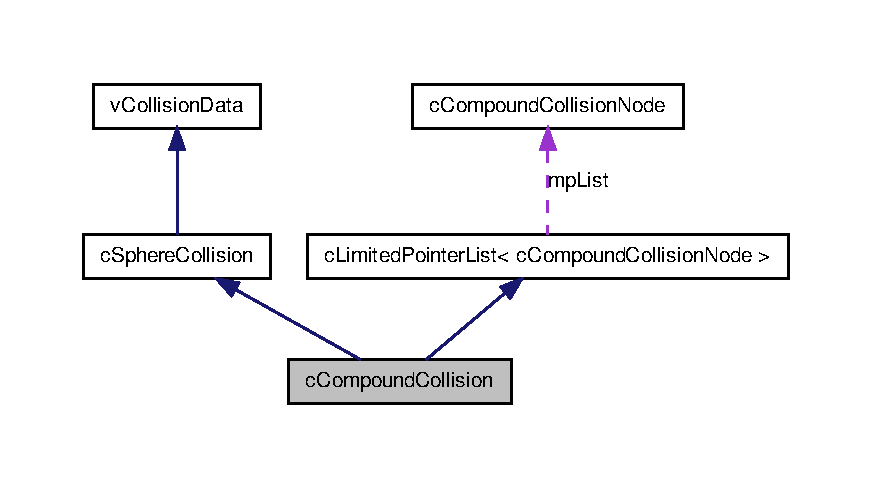
\includegraphics[width=400pt]{classc_compound_collision__coll__graph}
\end{center}
\end{figure}
\subsection*{Public Member Functions}
\begin{DoxyCompactItemize}
\item 
\hypertarget{classc_compound_collision_a6b8a94a617eb5198133d0759aeb3de02}{
\hyperlink{classc_compound_collision_a6b8a94a617eb5198133d0759aeb3de02}{cCompoundCollision} ()}
\label{classc_compound_collision_a6b8a94a617eb5198133d0759aeb3de02}

\begin{DoxyCompactList}\small\item\em Constructor creting a 0 length list. \end{DoxyCompactList}\item 
\hypertarget{classc_compound_collision_a8769934e6b4193ad31663288f8f55d0a}{
\hyperlink{classc_compound_collision_a8769934e6b4193ad31663288f8f55d0a}{cCompoundCollision} (uint32 liSize)}
\label{classc_compound_collision_a8769934e6b4193ad31663288f8f55d0a}

\begin{DoxyCompactList}\small\item\em Constructor creating a list of length liSize. \end{DoxyCompactList}\item 
\hypertarget{classc_compound_collision_ac95481f434fe511808ed362139442056}{
virtual \hyperlink{classc_compound_collision_ac95481f434fe511808ed362139442056}{$\sim$cCompoundCollision} ()}
\label{classc_compound_collision_ac95481f434fe511808ed362139442056}

\begin{DoxyCompactList}\small\item\em Destructor. \end{DoxyCompactList}\item 
\hypertarget{classc_compound_collision_ad54119082da305da69cce7c9b58e7135}{
\hyperlink{classc_compound_collision}{cCompoundCollision} $\ast$ \hyperlink{classc_compound_collision_ad54119082da305da69cce7c9b58e7135}{Compound} ()}
\label{classc_compound_collision_ad54119082da305da69cce7c9b58e7135}

\begin{DoxyCompactList}\small\item\em Will return a pointer if this object contains a Compound collision data objecty. Otherwise returns 0;. \end{DoxyCompactList}\item 
\hypertarget{classc_compound_collision_a0f0b6cd5120d20e6ad65a5ba2b27fc97}{
\hyperlink{classv_collision_data}{vCollisionData} $\ast$ \hyperlink{classc_compound_collision_a0f0b6cd5120d20e6ad65a5ba2b27fc97}{operator\mbox{[}$\,$\mbox{]}} (uint32 liPos)}
\label{classc_compound_collision_a0f0b6cd5120d20e6ad65a5ba2b27fc97}

\begin{DoxyCompactList}\small\item\em \mbox{[}\mbox{]} operator to access the \hyperlink{classv_collision_data}{vCollisionData} Objects within this \hyperlink{classc_compound_collision}{cCompoundCollision} Object. \end{DoxyCompactList}\item 
\hypertarget{classc_compound_collision_a0561694de30328b4aa20058ab36896a8}{
void \hyperlink{classc_compound_collision_a0561694de30328b4aa20058ab36896a8}{AddType} (\hyperlink{classv_collision_data}{vCollisionData} $\ast$lpOther)}
\label{classc_compound_collision_a0561694de30328b4aa20058ab36896a8}

\begin{DoxyCompactList}\small\item\em For adding a created \hyperlink{classv_collision_data}{vCollisionData} object. \hyperlink{classc_sphere_collision}{cSphereCollision}, \hyperlink{classc_mesh_collision}{cMeshCollision}, \hyperlink{classc_beam_collision}{cBeamCollision} etc. \end{DoxyCompactList}\item 
\hypertarget{classc_compound_collision_a83f2917503be59a302ffe5ac7ea5b83d}{
\hyperlink{classc_sphere_collision}{cSphereCollision} $\ast$ \hyperlink{classc_compound_collision_a83f2917503be59a302ffe5ac7ea5b83d}{AddType} (float lfSize)}
\label{classc_compound_collision_a83f2917503be59a302ffe5ac7ea5b83d}

\begin{DoxyCompactList}\small\item\em This will procedurally generate a Sphere or radius 1.0f;. \end{DoxyCompactList}\item 
\hypertarget{classc_compound_collision_ac3ab2e52fd2ea45debe26100e29183e4}{
\hyperlink{classc_beam_collision}{cBeamCollision} $\ast$ \hyperlink{classc_compound_collision_ac3ab2e52fd2ea45debe26100e29183e4}{AddType} (float lfLength, float lfRadius)}
\label{classc_compound_collision_ac3ab2e52fd2ea45debe26100e29183e4}

\begin{DoxyCompactList}\small\item\em This will procedurally generate a Beam of Radius lfRadius and Length lfLength. \end{DoxyCompactList}\item 
\hypertarget{classc_compound_collision_ab30aa4fa5730514f1c046676523b9f19}{
\hyperlink{classc_mesh_collision}{cMeshCollision} $\ast$ \hyperlink{classc_compound_collision_ab30aa4fa5730514f1c046676523b9f19}{AddType} (float $\ast$lpBounds)}
\label{classc_compound_collision_ab30aa4fa5730514f1c046676523b9f19}

\begin{DoxyCompactList}\small\item\em This will procedureally generate a Box collision object from the array of 6 floats lpBounds. see cGeneratedBoxCollision::BuildObject(float $\ast$lpBounds) for more information. \end{DoxyCompactList}\item 
\hypertarget{classc_compound_collision_a094a1e2b828fc8bd1ce0e5ab903125d6}{
\hyperlink{classc_mesh_collision}{cMeshCollision} $\ast$ \hyperlink{classc_compound_collision_a094a1e2b828fc8bd1ce0e5ab903125d6}{AddType} (float lfXP, float lfXN, float lfYP, float lfYN, float lfZP, float lfZN)}
\label{classc_compound_collision_a094a1e2b828fc8bd1ce0e5ab903125d6}

\begin{DoxyCompactList}\small\item\em This will procedurally generate a Box Collision object. This is the same as handing it a float pointer. \end{DoxyCompactList}\item 
\hypertarget{classc_compound_collision_a8b37e865b51fd5864582f8388ab4f1c4}{
\hyperlink{classc_beam_collision}{cBeamCollision} $\ast$ \hyperlink{classc_compound_collision_a8b37e865b51fd5864582f8388ab4f1c4}{AddType} (\hyperlink{classc_beam_mesh}{cBeamMesh} $\ast$lpBeam)}
\label{classc_compound_collision_a8b37e865b51fd5864582f8388ab4f1c4}

\begin{DoxyCompactList}\small\item\em This will make a Beam object to match a rendered Beam. (Nice and easy eh?) \end{DoxyCompactList}\item 
\hypertarget{classc_compound_collision_ad96f10a72496cb8879cf7b82d5403f81}{
uint8 \hyperlink{classc_compound_collision_ad96f10a72496cb8879cf7b82d5403f81}{Type} ()}
\label{classc_compound_collision_ad96f10a72496cb8879cf7b82d5403f81}

\begin{DoxyCompactList}\small\item\em Will return the Objects Type. \end{DoxyCompactList}\end{DoxyCompactItemize}


\subsection{Detailed Description}
The \hyperlink{classc_compound_collision}{cCompoundCollision} object is a type of \hyperlink{classv_collision_data}{vCollisionData} for combining multiple Collision Objects into a single object. This allows the user to construct a collision object out of several simpler objects. This makes it possible to produce 'concave' faces by using several objects with exclusively convex faces. It is a \hyperlink{classc_limited_pointer_list}{cLimitedPointerList} so can have the size of the array adjusted to store as many objects as are required. If there is a collision with any object within this compound Object then the \hyperlink{classc_compound_collision}{cCompoundCollision} object has collided. Negative Collision Objects will be added at a future date. Each Object within the \hyperlink{classc_compound_collision}{cCompoundCollision} Object has a \hyperlink{classc_matrix4}{cMatrix4} to allow it to be positioned and rotated as required. This class should either be started with a list size -\/ \hyperlink{classc_compound_collision_a8769934e6b4193ad31663288f8f55d0a}{cCompoundCollision(uint32 liSize)} -\/ or call the function \hyperlink{classc_limited_pointer_list_ab72b03a5d82ee318bf21d3102bdfecda}{Init(uint32 liSize)} before it is used. 
\hypertarget{classc_compound_collision_node}{
\section{cCompoundCollisionNode Class Reference}
\label{classc_compound_collision_node}\index{cCompoundCollisionNode@{cCompoundCollisionNode}}
}


This is the storage class for cCompouncCollision objects. You will not interact with it directly, but it should be mentioned to explain where the \hyperlink{classc_matrix4}{cMatrix4} comes from for objects within a \hyperlink{classc_compound_collision}{cCompoundCollision} Object.  


\subsection*{Public Member Functions}
\begin{DoxyCompactItemize}
\item 
\hypertarget{classc_compound_collision_node_ab3c55081c67d9cac8ea79f8b524ec696}{
\hyperlink{classc_compound_collision_node_ab3c55081c67d9cac8ea79f8b524ec696}{cCompoundCollisionNode} ()}
\label{classc_compound_collision_node_ab3c55081c67d9cac8ea79f8b524ec696}

\begin{DoxyCompactList}\small\item\em Constructor. \end{DoxyCompactList}\item 
\hypertarget{classc_compound_collision_node_acf2c370d49bf0f1b4be04c04348f4b4e}{
\hyperlink{classc_compound_collision_node_acf2c370d49bf0f1b4be04c04348f4b4e}{$\sim$cCompoundCollisionNode} ()}
\label{classc_compound_collision_node_acf2c370d49bf0f1b4be04c04348f4b4e}

\begin{DoxyCompactList}\small\item\em Destructor. \end{DoxyCompactList}\end{DoxyCompactItemize}
\subsection*{Friends}
\begin{DoxyCompactItemize}
\item 
\hypertarget{classc_compound_collision_node_adac1704bd2ebfcd3d16228685997db63}{
class \hyperlink{classc_compound_collision_node_adac1704bd2ebfcd3d16228685997db63}{cCompoundCollision}}
\label{classc_compound_collision_node_adac1704bd2ebfcd3d16228685997db63}

\end{DoxyCompactItemize}


\subsection{Detailed Description}
This is the storage class for cCompouncCollision objects. You will not interact with it directly, but it should be mentioned to explain where the \hyperlink{classc_matrix4}{cMatrix4} comes from for objects within a \hyperlink{classc_compound_collision}{cCompoundCollision} Object. 
\hypertarget{classc_event_handler}{
\section{cEventHandler Class Reference}
\label{classc_event_handler}\index{cEventHandler@{cEventHandler}}
}


This will handle events from the OS. Actually this will just store the Input data for the keyboard and mouse. It is easiest to access the input data using \_\-KEY and \_\-MOUSE. There can only be one \hyperlink{classc_event_handler}{cEventHandler}, created using \hyperlink{classc_event_handler_a8cf5519e1f3c5f6a6f79f9da75fb2750}{Instance()}.  




Collaboration diagram for cEventHandler:\nopagebreak
\begin{figure}[H]
\begin{center}
\leavevmode
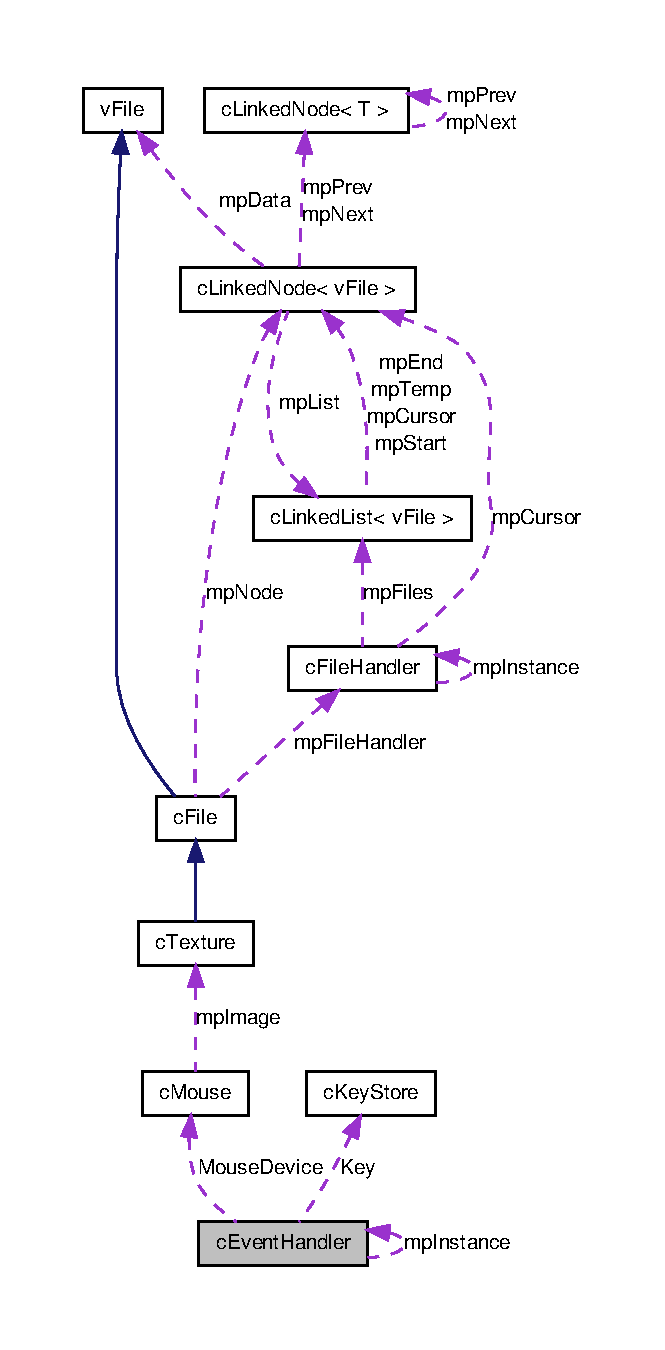
\includegraphics[width=257pt]{classc_event_handler__coll__graph}
\end{center}
\end{figure}
\subsection*{Static Public Member Functions}
\begin{DoxyCompactItemize}
\item 
\hypertarget{classc_event_handler_a8cf5519e1f3c5f6a6f79f9da75fb2750}{
static \hyperlink{classc_event_handler}{cEventHandler} $\ast$ \hyperlink{classc_event_handler_a8cf5519e1f3c5f6a6f79f9da75fb2750}{Instance} ()}
\label{classc_event_handler_a8cf5519e1f3c5f6a6f79f9da75fb2750}

\begin{DoxyCompactList}\small\item\em This will return a pointer to the current cEventhandler instance. If there is no instance it will create one. \end{DoxyCompactList}\end{DoxyCompactItemize}
\subsection*{Public Attributes}
\begin{DoxyCompactItemize}
\item 
\hypertarget{classc_event_handler_a53ba15cada383fb64c9918d8ce923585}{
\hyperlink{classc_key_store}{cKeyStore} \hyperlink{classc_event_handler_a53ba15cada383fb64c9918d8ce923585}{Key}}
\label{classc_event_handler_a53ba15cada383fb64c9918d8ce923585}

\begin{DoxyCompactList}\small\item\em This will store all the keyboard input data. see \_\-KEY. \end{DoxyCompactList}\item 
\hypertarget{classc_event_handler_a5d871cf2ddea710db2b4daed30cd1866}{
\hyperlink{classc_mouse}{cMouse} \hyperlink{classc_event_handler_a5d871cf2ddea710db2b4daed30cd1866}{MouseDevice}}
\label{classc_event_handler_a5d871cf2ddea710db2b4daed30cd1866}

\begin{DoxyCompactList}\small\item\em This will store the mouse input data. see \_\-MOUSE. \end{DoxyCompactList}\end{DoxyCompactItemize}


\subsection{Detailed Description}
This will handle events from the OS. Actually this will just store the Input data for the keyboard and mouse. It is easiest to access the input data using \_\-KEY and \_\-MOUSE. There can only be one \hyperlink{classc_event_handler}{cEventHandler}, created using \hyperlink{classc_event_handler_a8cf5519e1f3c5f6a6f79f9da75fb2750}{Instance()}. 
\hypertarget{classc_face}{
\section{cFace Class Reference}
\label{classc_face}\index{cFace@{cFace}}
}


This class will store data about faces for a 3D Mesh. This can be used for Models, Collision Meshes or any other object using 3D Faces. Includes code for loading and saving the object types to and from IMF Files. Uses \hyperlink{classc_vertex}{cVertex} and \hyperlink{classc_plane}{cPlane} to store the data.  




Inheritance diagram for cFace:
\nopagebreak
\begin{figure}[H]
\begin{center}
\leavevmode
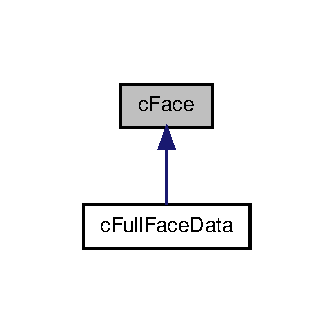
\includegraphics[width=160pt]{classc_face__inherit__graph}
\end{center}
\end{figure}


Collaboration diagram for cFace:
\nopagebreak
\begin{figure}[H]
\begin{center}
\leavevmode
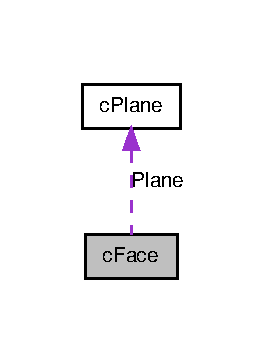
\includegraphics[width=194pt]{classc_face__coll__graph}
\end{center}
\end{figure}
\subsection*{Public Member Functions}
\begin{DoxyCompactItemize}
\item 
\hyperlink{classc_face}{cFace} \& \hyperlink{classc_face_aff51f522716a340fe0f0b3c55ab68bff}{operator=} (\hyperlink{classc_face}{cFace} \&lpOther)
\item 
uint32 \hyperlink{classc_face_ac2da0ca5e4269e12016b74c6443cde32}{FileSize} ()
\item 
void \hyperlink{classc_face_a1b1ff8e5ec5f30b1140e7f1e71086ed5}{OutputIMFFace} (ofstream \&FileStream)
\item 
void \hyperlink{classc_face_a8a39f8e4a8bf051dc67c7f55a88d636b}{LoadIMFFace} (ifstream \&FileStream)
\end{DoxyCompactItemize}
\subsection*{Public Attributes}
\begin{DoxyCompactItemize}
\item 
\hyperlink{classc_vertex}{cVertex} \hyperlink{classc_face_ae08ccc2952b022dce6848628649d61c8}{Verteces} \mbox{[}3\mbox{]}
\item 
\hyperlink{classc_plane}{cPlane} \hyperlink{classc_face_aa61d6dca6df8211a1a816edbf303bd27}{Plane}
\end{DoxyCompactItemize}


\subsection{Detailed Description}
This class will store data about faces for a 3D Mesh. This can be used for Models, Collision Meshes or any other object using 3D Faces. Includes code for loading and saving the object types to and from IMF Files. Uses \hyperlink{classc_vertex}{cVertex} and \hyperlink{classc_plane}{cPlane} to store the data. 

Definition at line 7 of file WTcFace.h.



\subsection{Member Function Documentation}
\hypertarget{classc_face_ac2da0ca5e4269e12016b74c6443cde32}{
\index{cFace@{cFace}!FileSize@{FileSize}}
\index{FileSize@{FileSize}!cFace@{cFace}}
\subsubsection[{FileSize}]{\setlength{\rightskip}{0pt plus 5cm}uint32 cFace::FileSize (
\begin{DoxyParamCaption}
{}
\end{DoxyParamCaption}
)}}
\label{classc_face_ac2da0ca5e4269e12016b74c6443cde32}


Reimplemented in \hyperlink{classc_full_face_data_a53a99ced9de4ecdede38b2e8d63458e9}{cFullFaceData}.



Definition at line 12 of file WTcFace.cpp.

\hypertarget{classc_face_a8a39f8e4a8bf051dc67c7f55a88d636b}{
\index{cFace@{cFace}!LoadIMFFace@{LoadIMFFace}}
\index{LoadIMFFace@{LoadIMFFace}!cFace@{cFace}}
\subsubsection[{LoadIMFFace}]{\setlength{\rightskip}{0pt plus 5cm}void cFace::LoadIMFFace (
\begin{DoxyParamCaption}
\item[{ifstream \&}]{FileStream}
\end{DoxyParamCaption}
)}}
\label{classc_face_a8a39f8e4a8bf051dc67c7f55a88d636b}


Definition at line 33 of file WTcFace.cpp.

\hypertarget{classc_face_aff51f522716a340fe0f0b3c55ab68bff}{
\index{cFace@{cFace}!operator=@{operator=}}
\index{operator=@{operator=}!cFace@{cFace}}
\subsubsection[{operator=}]{\setlength{\rightskip}{0pt plus 5cm}{\bf cFace} \& cFace::operator= (
\begin{DoxyParamCaption}
\item[{{\bf cFace} \&}]{lpOther}
\end{DoxyParamCaption}
)}}
\label{classc_face_aff51f522716a340fe0f0b3c55ab68bff}


Definition at line 3 of file WTcFace.cpp.

\hypertarget{classc_face_a1b1ff8e5ec5f30b1140e7f1e71086ed5}{
\index{cFace@{cFace}!OutputIMFFace@{OutputIMFFace}}
\index{OutputIMFFace@{OutputIMFFace}!cFace@{cFace}}
\subsubsection[{OutputIMFFace}]{\setlength{\rightskip}{0pt plus 5cm}void cFace::OutputIMFFace (
\begin{DoxyParamCaption}
\item[{ofstream \&}]{FileStream}
\end{DoxyParamCaption}
)}}
\label{classc_face_a1b1ff8e5ec5f30b1140e7f1e71086ed5}


Definition at line 24 of file WTcFace.cpp.



\subsection{Member Data Documentation}
\hypertarget{classc_face_aa61d6dca6df8211a1a816edbf303bd27}{
\index{cFace@{cFace}!Plane@{Plane}}
\index{Plane@{Plane}!cFace@{cFace}}
\subsubsection[{Plane}]{\setlength{\rightskip}{0pt plus 5cm}{\bf cPlane} {\bf cFace::Plane}}}
\label{classc_face_aa61d6dca6df8211a1a816edbf303bd27}


Definition at line 12 of file WTcFace.h.

\hypertarget{classc_face_ae08ccc2952b022dce6848628649d61c8}{
\index{cFace@{cFace}!Verteces@{Verteces}}
\index{Verteces@{Verteces}!cFace@{cFace}}
\subsubsection[{Verteces}]{\setlength{\rightskip}{0pt plus 5cm}{\bf cVertex} {\bf cFace::Verteces}\mbox{[}3\mbox{]}}}
\label{classc_face_ae08ccc2952b022dce6848628649d61c8}


Definition at line 11 of file WTcFace.h.


\hypertarget{classc_file}{
\section{cFile Class Reference}
\label{classc_file}\index{cFile@{cFile}}
}


This is the base code for files to be loaded from a hdd. Any file object loaded from a hddvshould inherit this class. It is best used for media files. This code will automatically add newly loaded files to \hyperlink{classc_file_handler}{cFileHandler}. The files can be loaded using the filename or if loaded from an IMF file using the reference for each file.  




Collaboration diagram for cFile:\nopagebreak
\begin{figure}[H]
\begin{center}
\leavevmode
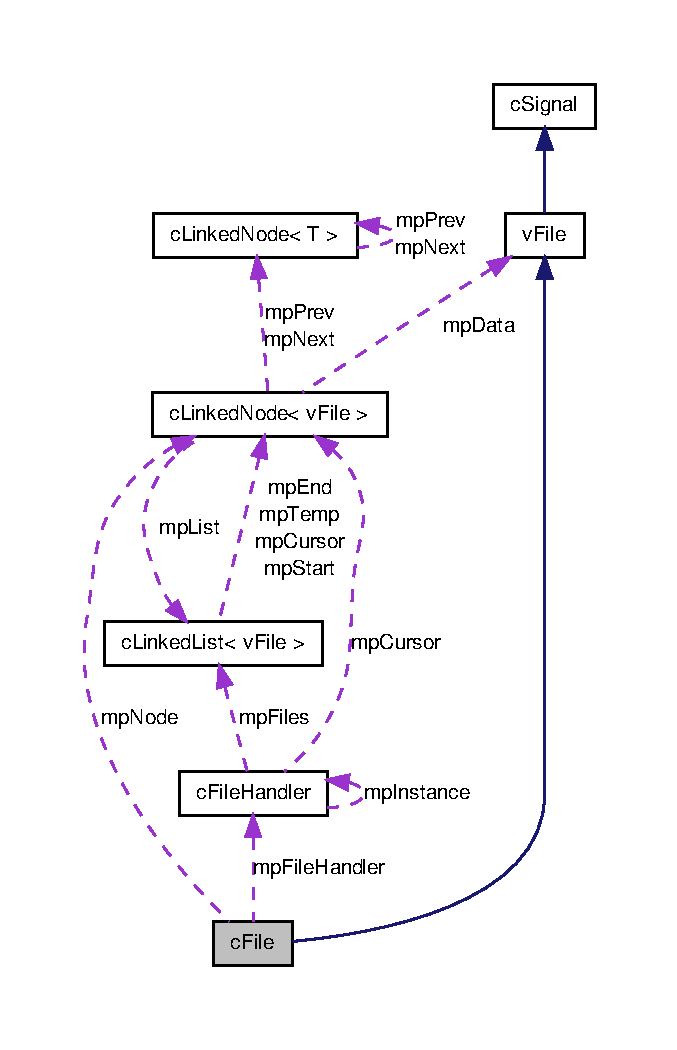
\includegraphics[width=320pt]{classc_file__coll__graph}
\end{center}
\end{figure}
\subsection*{Public Member Functions}
\begin{DoxyCompactItemize}
\item 
\hypertarget{classc_file_a5bb81f36e954af61b581e3c1fd06e0de}{
\hyperlink{classc_file_a5bb81f36e954af61b581e3c1fd06e0de}{cFile} ()}
\label{classc_file_a5bb81f36e954af61b581e3c1fd06e0de}

\begin{DoxyCompactList}\small\item\em This constructor will automatically load the file from memory and add it to the list in cFilehandler. \end{DoxyCompactList}\item 
\hypertarget{classc_file_a7224559b2485e53608bd6ba9e21d1122}{
char $\ast$ \hyperlink{classc_file_a7224559b2485e53608bd6ba9e21d1122}{FileName} ()}
\label{classc_file_a7224559b2485e53608bd6ba9e21d1122}

\begin{DoxyCompactList}\small\item\em This will return the files filename. \end{DoxyCompactList}\item 
\hypertarget{classc_file_aa5891f6208183a26e7fde7d8dee62ffc}{
void \hyperlink{classc_file_aa5891f6208183a26e7fde7d8dee62ffc}{Load} ()}
\label{classc_file_aa5891f6208183a26e7fde7d8dee62ffc}

\begin{DoxyCompactList}\small\item\em This is the function that will actually load the file from a hdd. \end{DoxyCompactList}\item 
\hypertarget{classc_file_ab2e74ccc027ccb92ea577cd7bb9b5f5c}{
void \hyperlink{classc_file_ab2e74ccc027ccb92ea577cd7bb9b5f5c}{Delete} ()}
\label{classc_file_ab2e74ccc027ccb92ea577cd7bb9b5f5c}

\begin{DoxyCompactList}\small\item\em This will delete the file from memory. \end{DoxyCompactList}\end{DoxyCompactItemize}
\subsection*{Public Attributes}
\begin{DoxyCompactItemize}
\item 
\hypertarget{classc_file_aed51bea596b50e6c8a03dd1593298681}{
\hyperlink{classc_linked_node}{cLinkedNode}$<$ \hyperlink{classv_file}{vFile} $>$ $\ast$ \hyperlink{classc_file_aed51bea596b50e6c8a03dd1593298681}{mpNode}}
\label{classc_file_aed51bea596b50e6c8a03dd1593298681}

\begin{DoxyCompactList}\small\item\em This is a pointer to the \hyperlink{classc_linked_node}{cLinkedNode} which owns this file. \end{DoxyCompactList}\item 
\hypertarget{classc_file_a5e3add41cacddcc489ca9aa185e3b066}{
char \hyperlink{classc_file_a5e3add41cacddcc489ca9aa185e3b066}{mpFileName} \mbox{[}64\mbox{]}}
\label{classc_file_a5e3add41cacddcc489ca9aa185e3b066}

\begin{DoxyCompactList}\small\item\em This will store the files filename. \end{DoxyCompactList}\end{DoxyCompactItemize}
\subsection*{Protected Attributes}
\begin{DoxyCompactItemize}
\item 
\hypertarget{classc_file_ae54eca20c29d2fcd5649aac33d1dba9a}{
\hyperlink{classc_file_handler}{cFileHandler} $\ast$ \hyperlink{classc_file_ae54eca20c29d2fcd5649aac33d1dba9a}{mpFileHandler}}
\label{classc_file_ae54eca20c29d2fcd5649aac33d1dba9a}

\begin{DoxyCompactList}\small\item\em This is a pointer to the \hyperlink{classc_file_handler}{cFileHandler} which owns this file. \end{DoxyCompactList}\end{DoxyCompactItemize}
\subsection*{Friends}
\begin{DoxyCompactItemize}
\item 
\hypertarget{classc_file_a70d0eacda2243b6345feb400aef70378}{
class \hyperlink{classc_file_a70d0eacda2243b6345feb400aef70378}{cFileHandler}}
\label{classc_file_a70d0eacda2243b6345feb400aef70378}

\end{DoxyCompactItemize}


\subsection{Detailed Description}
This is the base code for files to be loaded from a hdd. Any file object loaded from a hddvshould inherit this class. It is best used for media files. This code will automatically add newly loaded files to \hyperlink{classc_file_handler}{cFileHandler}. The files can be loaded using the filename or if loaded from an IMF file using the reference for each file. 
\hypertarget{classc_file_handler}{
\section{cFileHandler Class Reference}
\label{classc_file_handler}\index{cFileHandler@{cFileHandler}}
}


This is the handler for the file system. This handles all files loaded from a hdd. It will give allow processes to use files loaded else where, using either the filenames or if loaded from an IMF a file reference. The files are stored in the list mpFiles.  




Collaboration diagram for cFileHandler:
\nopagebreak
\begin{figure}[H]
\begin{center}
\leavevmode
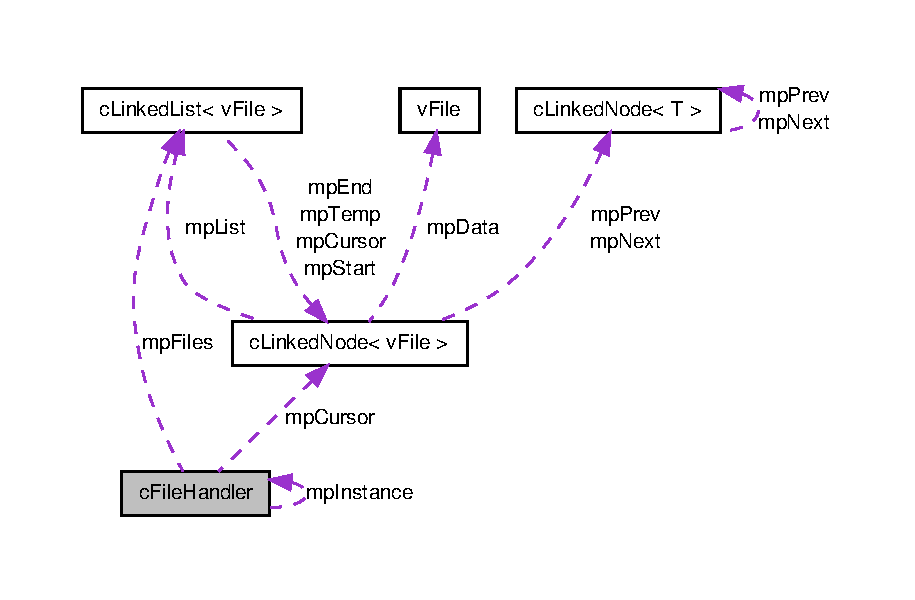
\includegraphics[width=400pt]{classc_file_handler__coll__graph}
\end{center}
\end{figure}
\subsection*{Public Member Functions}
\begin{DoxyCompactItemize}
\item 
\hyperlink{classc_file_handler_a88dd9099f9332245a2f2fc8a3eb8abc5}{$\sim$cFileHandler} ()
\item 
void \hyperlink{classc_file_handler_a87ff1f0cc36ef46514f77826eaf04453}{Reload} ()
\begin{DoxyCompactList}\small\item\em This will reload all the files from a hdd into memory. (Note this is not currently complete). \item\end{DoxyCompactList}\item 
void \hyperlink{classc_file_handler_a610399fa5d6bdb45de1d3cdc4dcb4c3c}{Unload} ()
\begin{DoxyCompactList}\small\item\em This will remove all the files from memory. (Note this is not currently complete). \item\end{DoxyCompactList}\item 
void $\ast$ \hyperlink{classc_file_handler_a3d2432f40a2d8f2fed223b6ad508b7df}{File} (const char $\ast$lpFilename)
\begin{DoxyCompactList}\small\item\em This will return a pointer to a file with the filename or file refernce lpFilename. \item\end{DoxyCompactList}\item 
\hyperlink{classc_linked_node}{cLinkedNode}$<$ \hyperlink{classv_file}{vFile} $>$ $\ast$ \hyperlink{classc_file_handler_a30b1285eaca092f8417c3f1750f60559}{Add} (\hyperlink{classv_file}{vFile} $\ast$lpNew)
\begin{DoxyCompactList}\small\item\em This will add the file pointed to by lpNew to the current file list mpFile. \item\end{DoxyCompactList}\item 
void \hyperlink{classc_file_handler_a2701aa77518747a401b51e0c38ba1cd1}{Delete} (\hyperlink{classc_linked_node}{cLinkedNode}$<$ \hyperlink{classv_file}{vFile} $>$ $\ast$lpNode)
\begin{DoxyCompactList}\small\item\em This will delete the file owned by lpNode from the file list mpFile. \item\end{DoxyCompactList}\end{DoxyCompactItemize}
\subsection*{Static Public Member Functions}
\begin{DoxyCompactItemize}
\item 
static \hyperlink{classc_file_handler}{cFileHandler} $\ast$ \hyperlink{classc_file_handler_a99495051a1a41a763113aca5292023b9}{Instance} ()
\begin{DoxyCompactList}\small\item\em This will return a pointer to the current \hyperlink{classc_file_handler}{cFileHandler}. If there is no current instance it will create one and return the pointer. \item\end{DoxyCompactList}\end{DoxyCompactItemize}


\subsection{Detailed Description}
This is the handler for the file system. This handles all files loaded from a hdd. It will give allow processes to use files loaded else where, using either the filenames or if loaded from an IMF a file reference. The files are stored in the list mpFiles. 

Definition at line 10 of file WTcFileHandler.h.



\subsection{Constructor \& Destructor Documentation}
\hypertarget{classc_file_handler_a88dd9099f9332245a2f2fc8a3eb8abc5}{
\index{cFileHandler@{cFileHandler}!$\sim$cFileHandler@{$\sim$cFileHandler}}
\index{$\sim$cFileHandler@{$\sim$cFileHandler}!cFileHandler@{cFileHandler}}
\subsubsection[{$\sim$cFileHandler}]{\setlength{\rightskip}{0pt plus 5cm}cFileHandler::$\sim$cFileHandler (
\begin{DoxyParamCaption}
{}
\end{DoxyParamCaption}
)}}
\label{classc_file_handler_a88dd9099f9332245a2f2fc8a3eb8abc5}


Definition at line 24 of file WTcFileHandler.cpp.



\subsection{Member Function Documentation}
\hypertarget{classc_file_handler_a30b1285eaca092f8417c3f1750f60559}{
\index{cFileHandler@{cFileHandler}!Add@{Add}}
\index{Add@{Add}!cFileHandler@{cFileHandler}}
\subsubsection[{Add}]{\setlength{\rightskip}{0pt plus 5cm}{\bf cLinkedNode}$<$ {\bf vFile} $>$ $\ast$ cFileHandler::Add (
\begin{DoxyParamCaption}
\item[{{\bf vFile} $\ast$}]{lpNew}
\end{DoxyParamCaption}
)}}
\label{classc_file_handler_a30b1285eaca092f8417c3f1750f60559}


This will add the file pointed to by lpNew to the current file list mpFile. 



Definition at line 43 of file WTcFileHandler.cpp.

\hypertarget{classc_file_handler_a2701aa77518747a401b51e0c38ba1cd1}{
\index{cFileHandler@{cFileHandler}!Delete@{Delete}}
\index{Delete@{Delete}!cFileHandler@{cFileHandler}}
\subsubsection[{Delete}]{\setlength{\rightskip}{0pt plus 5cm}void cFileHandler::Delete (
\begin{DoxyParamCaption}
\item[{{\bf cLinkedNode}$<$ {\bf vFile} $>$ $\ast$}]{lpNode}
\end{DoxyParamCaption}
)}}
\label{classc_file_handler_a2701aa77518747a401b51e0c38ba1cd1}


This will delete the file owned by lpNode from the file list mpFile. 



Definition at line 52 of file WTcFileHandler.cpp.

\hypertarget{classc_file_handler_a3d2432f40a2d8f2fed223b6ad508b7df}{
\index{cFileHandler@{cFileHandler}!File@{File}}
\index{File@{File}!cFileHandler@{cFileHandler}}
\subsubsection[{File}]{\setlength{\rightskip}{0pt plus 5cm}void $\ast$ cFileHandler::File (
\begin{DoxyParamCaption}
\item[{const char $\ast$}]{lpFilename}
\end{DoxyParamCaption}
)}}
\label{classc_file_handler_a3d2432f40a2d8f2fed223b6ad508b7df}


This will return a pointer to a file with the filename or file refernce lpFilename. 



Definition at line 9 of file WTcFileHandler.cpp.

\hypertarget{classc_file_handler_a99495051a1a41a763113aca5292023b9}{
\index{cFileHandler@{cFileHandler}!Instance@{Instance}}
\index{Instance@{Instance}!cFileHandler@{cFileHandler}}
\subsubsection[{Instance}]{\setlength{\rightskip}{0pt plus 5cm}{\bf cFileHandler} $\ast$ cFileHandler::Instance (
\begin{DoxyParamCaption}
{}
\end{DoxyParamCaption}
)\hspace{0.3cm}{\ttfamily  \mbox{[}static\mbox{]}}}}
\label{classc_file_handler_a99495051a1a41a763113aca5292023b9}


This will return a pointer to the current \hyperlink{classc_file_handler}{cFileHandler}. If there is no current instance it will create one and return the pointer. 



Definition at line 33 of file WTcFileHandler.cpp.

\hypertarget{classc_file_handler_a87ff1f0cc36ef46514f77826eaf04453}{
\index{cFileHandler@{cFileHandler}!Reload@{Reload}}
\index{Reload@{Reload}!cFileHandler@{cFileHandler}}
\subsubsection[{Reload}]{\setlength{\rightskip}{0pt plus 5cm}void cFileHandler::Reload (
\begin{DoxyParamCaption}
{}
\end{DoxyParamCaption}
)}}
\label{classc_file_handler_a87ff1f0cc36ef46514f77826eaf04453}


This will reload all the files from a hdd into memory. (Note this is not currently complete). 



Definition at line 39 of file WTcFileHandler.cpp.

\hypertarget{classc_file_handler_a610399fa5d6bdb45de1d3cdc4dcb4c3c}{
\index{cFileHandler@{cFileHandler}!Unload@{Unload}}
\index{Unload@{Unload}!cFileHandler@{cFileHandler}}
\subsubsection[{Unload}]{\setlength{\rightskip}{0pt plus 5cm}void cFileHandler::Unload (
\begin{DoxyParamCaption}
{}
\end{DoxyParamCaption}
)}}
\label{classc_file_handler_a610399fa5d6bdb45de1d3cdc4dcb4c3c}


This will remove all the files from memory. (Note this is not currently complete). 



Definition at line 41 of file WTcFileHandler.cpp.


\hypertarget{classc_float_attribute_store}{
\section{cFloatAttributeStore Class Reference}
\label{classc_float_attribute_store}\index{cFloatAttributeStore@{cFloatAttributeStore}}
}


More Specific Base class for Attribute Handling classes. Suitable for float Variables. see \hyperlink{classc_attribute_array1}{cAttributeArray1}, \hyperlink{classc_attribute_array2}{cAttributeArray2}, \hyperlink{classc_attribute_array3}{cAttributeArray3}, \hyperlink{classc_attribute_array4}{cAttributeArray4}.  




Collaboration diagram for cFloatAttributeStore:\nopagebreak
\begin{figure}[H]
\begin{center}
\leavevmode
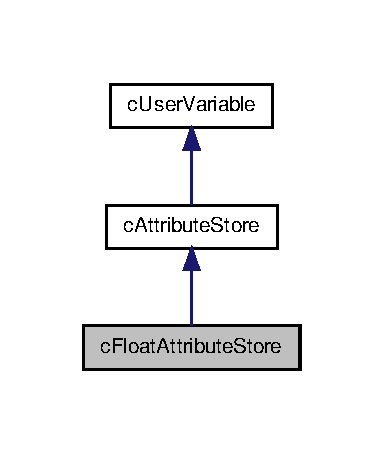
\includegraphics[width=184pt]{classc_float_attribute_store__coll__graph}
\end{center}
\end{figure}
\subsection*{Public Member Functions}
\begin{DoxyCompactItemize}
\item 
\hypertarget{classc_float_attribute_store_af9721a74ced818c5ae1aee3043b9a6bb}{
void \hyperlink{classc_float_attribute_store_af9721a74ced818c5ae1aee3043b9a6bb}{DataValue} (void $\ast$lpData, uint32 liElements)}
\label{classc_float_attribute_store_af9721a74ced818c5ae1aee3043b9a6bb}

\begin{DoxyCompactList}\small\item\em This will Set the Array of Data an Attribute Variable will Use. This will copy the data. It will not automatically update, but the data can be deallocated at any time. \end{DoxyCompactList}\item 
\hypertarget{classc_float_attribute_store_a930627974932e8bca72f6c4dd70c68a8}{
void \hyperlink{classc_float_attribute_store_a930627974932e8bca72f6c4dd70c68a8}{DataPointer} (void $\ast$lpData, uint32 liElements)}
\label{classc_float_attribute_store_a930627974932e8bca72f6c4dd70c68a8}

\begin{DoxyCompactList}\small\item\em This will Set the Array of Data an Attribute Variable will Use. This will not copy the data, but will store a pointer to the data. It will automatically update, but the data passed to it should not be deallocated while the shader is in use. \end{DoxyCompactList}\item 
\hypertarget{classc_float_attribute_store_acf7c84372c2259cd6921013083730e4b}{
void $\ast$ \hyperlink{classc_float_attribute_store_acf7c84372c2259cd6921013083730e4b}{Data} ()}
\label{classc_float_attribute_store_acf7c84372c2259cd6921013083730e4b}

\begin{DoxyCompactList}\small\item\em This will return the data the Function is pointing at. \end{DoxyCompactList}\end{DoxyCompactItemize}


\subsection{Detailed Description}
More Specific Base class for Attribute Handling classes. Suitable for float Variables. see \hyperlink{classc_attribute_array1}{cAttributeArray1}, \hyperlink{classc_attribute_array2}{cAttributeArray2}, \hyperlink{classc_attribute_array3}{cAttributeArray3}, \hyperlink{classc_attribute_array4}{cAttributeArray4}. 
\hypertarget{classc_float_uniform_store}{
\section{cFloatUniformStore Class Reference}
\label{classc_float_uniform_store}\index{cFloatUniformStore@{cFloatUniformStore}}
}


More Specific Base class for Uniform Handling classes. Suitable for float Variables. see \hyperlink{classc_uniform_vector1}{cUniformVector1}, \hyperlink{classc_uniform_vector2}{cUniformVector2}, \hyperlink{classc_uniform_vector3}{cUniformVector3}, \hyperlink{classc_uniform_vector4}{cUniformVector4}.  




Collaboration diagram for cFloatUniformStore:\nopagebreak
\begin{figure}[H]
\begin{center}
\leavevmode
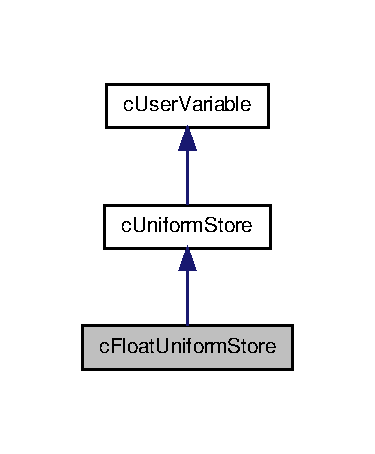
\includegraphics[width=180pt]{classc_float_uniform_store__coll__graph}
\end{center}
\end{figure}
\subsection*{Public Member Functions}
\begin{DoxyCompactItemize}
\item 
\hypertarget{classc_float_uniform_store_a95ff7fe17352d7da93382001706db97d}{
void \hyperlink{classc_float_uniform_store_a95ff7fe17352d7da93382001706db97d}{DataPointer} (void $\ast$lpData)}
\label{classc_float_uniform_store_a95ff7fe17352d7da93382001706db97d}

\begin{DoxyCompactList}\small\item\em This will Set the Data a Uniform Variable will Use. This will not copy the data, but will store a pointer to the data. It will automatically update, but the data passed to it should not be deallocated while the shader is in use. \end{DoxyCompactList}\item 
\hypertarget{classc_float_uniform_store_acdd11db6d22fbcd1005053c327fb93ba}{
void $\ast$ \hyperlink{classc_float_uniform_store_acdd11db6d22fbcd1005053c327fb93ba}{Data} ()}
\label{classc_float_uniform_store_acdd11db6d22fbcd1005053c327fb93ba}

\begin{DoxyCompactList}\small\item\em This will return the data the Function is pointing at. \end{DoxyCompactList}\end{DoxyCompactItemize}


\subsection{Detailed Description}
More Specific Base class for Uniform Handling classes. Suitable for float Variables. see \hyperlink{classc_uniform_vector1}{cUniformVector1}, \hyperlink{classc_uniform_vector2}{cUniformVector2}, \hyperlink{classc_uniform_vector3}{cUniformVector3}, \hyperlink{classc_uniform_vector4}{cUniformVector4}. 
\hypertarget{classc_font}{
\section{cFont Class Reference}
\label{classc_font}\index{cFont@{cFont}}
}


This class will store the data for a Font ready to be used for rendering \hyperlink{classc_text}{cText}. This should come from an IMF file and be composed of an image of 93 character images stacked vertically. This is a file class and should be handled entirely by the engine.  




Collaboration diagram for cFont:\nopagebreak
\begin{figure}[H]
\begin{center}
\leavevmode
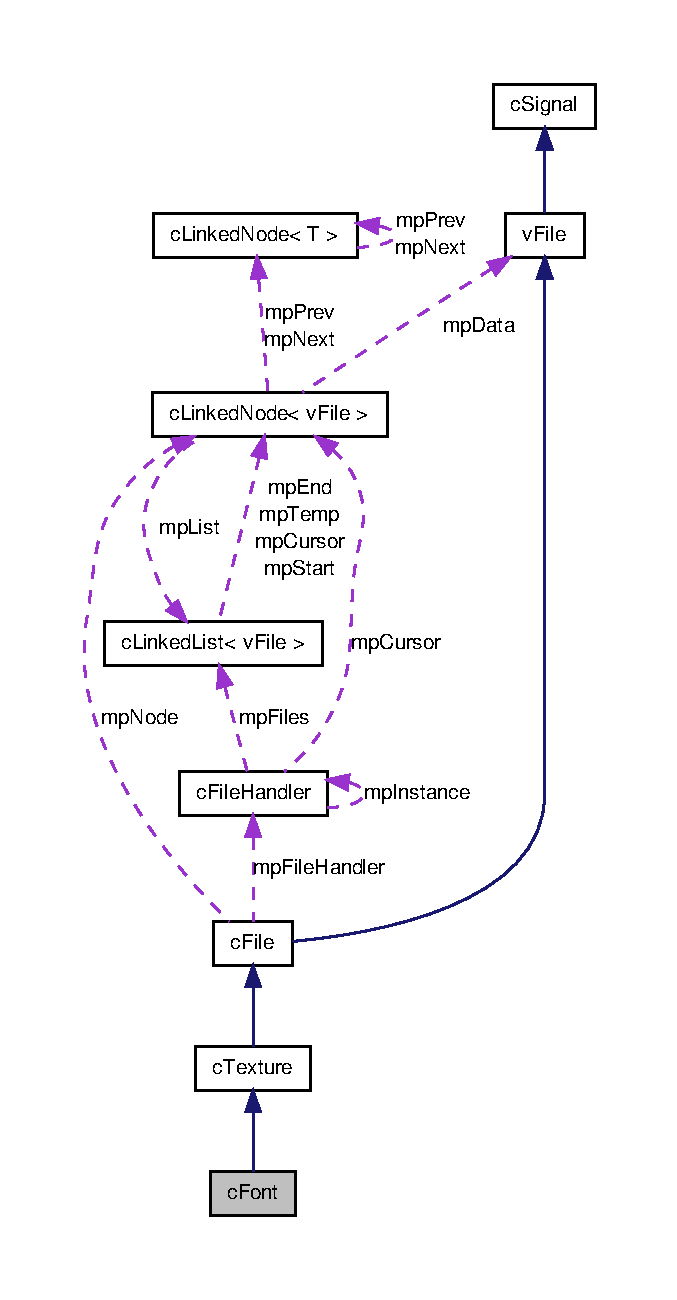
\includegraphics[width=320pt]{classc_font__coll__graph}
\end{center}
\end{figure}
\subsection*{Public Member Functions}
\begin{DoxyCompactItemize}
\item 
\hypertarget{classc_font_a3fa379c0126af4edd8c4f7bb39507a13}{
uint32 \hyperlink{classc_font_a3fa379c0126af4edd8c4f7bb39507a13}{Height} ()}
\label{classc_font_a3fa379c0126af4edd8c4f7bb39507a13}

\begin{DoxyCompactList}\small\item\em Returns the \hyperlink{classc_texture}{cTexture} Height. \end{DoxyCompactList}\end{DoxyCompactItemize}


\subsection{Detailed Description}
This class will store the data for a Font ready to be used for rendering \hyperlink{classc_text}{cText}. This should come from an IMF file and be composed of an image of 93 character images stacked vertically. This is a file class and should be handled entirely by the engine. 
\hypertarget{classc_frame_rate}{
\section{cFrameRate Class Reference}
\label{classc_frame_rate}\index{cFrameRate@{cFrameRate}}
}


This class will store data for controlling the Frame Rate. There are several settings that can be adjusted:\par
 Processes Per Frame:\par
 \par
 Frames Per Second:\par
 \par
 Frame Time and Process Time:\par
 These are the amount of time that passes every Frame and Process Cycle measured in seconds. Multiplying any distances moved by this will convert them into distance per second. This allows the user to change the running frame rate without affecting the speed the user experiences. If the Frame rate and Process Rate are not going to be changed this can be ignored.  




Collaboration diagram for cFrameRate:
\nopagebreak
\begin{figure}[H]
\begin{center}
\leavevmode
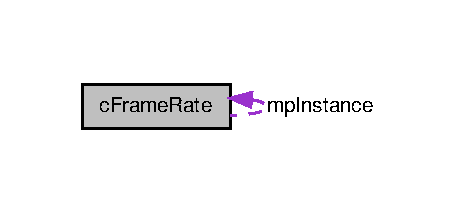
\includegraphics[width=220pt]{classc_frame_rate__coll__graph}
\end{center}
\end{figure}
\subsection*{Public Member Functions}
\begin{DoxyCompactItemize}
\item 
void \hyperlink{classc_frame_rate_a11d2578dfcb6eb2fea0bb331b7188dfe}{SetFrameRate} (uint8 lfFramesPerSecond)
\begin{DoxyCompactList}\small\item\em This is the number of Frames that will be rendered each second. This results in smooth consistent timings for every Process Cycle and Rendered Frame. This is best set to 60 / 70 though in extreme cases it can be set to 30. Rendering is very compoutationally expensive, so should be maintained at the lowest rate to produce a smooth visual image. \item\end{DoxyCompactList}\item 
void \hyperlink{classc_frame_rate_afb2bce05079fe1bc1e7b3ac3295fd692}{SetProcessesPerFrame} (uint8 liPPS)
\begin{DoxyCompactList}\small\item\em This is the number of times the Process cycle will be run for every rendered frame. Rendering is very slow and CPU intensive compared to the Procesing cycle. The Human eye cannot differentiate between very fast rendering rates, but increased numbers of processing cycles will increase accuracy of collisions and make events smoother. \item\end{DoxyCompactList}\item 
float \hyperlink{classc_frame_rate_a6af788062fd7f1cff658e19ca790219c}{FrameTime} ()
\begin{DoxyCompactList}\small\item\em this will return the amount of time that passes for every rendered frame. \item\end{DoxyCompactList}\item 
float \hyperlink{classc_frame_rate_ac314f1e240949dc74bd51730748ce1b2}{ProcessTime} ()
\begin{DoxyCompactList}\small\item\em This is the amount of time that passes every Process Cycle measured in seconds. Multiplying any distances moved by this will convert them into distance per second. This allows the user to change the running frame rate without affecting the speed the user experiences. If the Frame rate and Process Rate are not going to be changed this can be ignored. \item\end{DoxyCompactList}\item 
uint8 \hyperlink{classc_frame_rate_ab450d4c204172469695433474227bd19}{FramesPerSecond} ()
\begin{DoxyCompactList}\small\item\em This will return the current set number of Frames per Second. \item\end{DoxyCompactList}\item 
uint8 \hyperlink{classc_frame_rate_ab1b0bc7a9801cbea5d8036203a0a9ee4}{ProcessesPerFrame} ()
\begin{DoxyCompactList}\small\item\em this will return the current set number of Process Cycles per Rendered Frame. \item\end{DoxyCompactList}\end{DoxyCompactItemize}
\subsection*{Static Public Member Functions}
\begin{DoxyCompactItemize}
\item 
static \hyperlink{classc_frame_rate}{cFrameRate} $\ast$ \hyperlink{classc_frame_rate_a843b42d98bb70a1bc566a367b47d7fc3}{Instance} ()
\begin{DoxyCompactList}\small\item\em This will return a pointer to the current \hyperlink{classc_frame_rate}{cFrameRate} Object. \item\end{DoxyCompactList}\end{DoxyCompactItemize}


\subsection{Detailed Description}
This class will store data for controlling the Frame Rate. There are several settings that can be adjusted:\par
 Processes Per Frame:\par
 \par
 Frames Per Second:\par
 \par
 Frame Time and Process Time:\par
 These are the amount of time that passes every Frame and Process Cycle measured in seconds. Multiplying any distances moved by this will convert them into distance per second. This allows the user to change the running frame rate without affecting the speed the user experiences. If the Frame rate and Process Rate are not going to be changed this can be ignored. 

Definition at line 13 of file WTcFrameRate.h.



\subsection{Member Function Documentation}
\hypertarget{classc_frame_rate_ab450d4c204172469695433474227bd19}{
\index{cFrameRate@{cFrameRate}!FramesPerSecond@{FramesPerSecond}}
\index{FramesPerSecond@{FramesPerSecond}!cFrameRate@{cFrameRate}}
\subsubsection[{FramesPerSecond}]{\setlength{\rightskip}{0pt plus 5cm}uint8 cFrameRate::FramesPerSecond (
\begin{DoxyParamCaption}
{}
\end{DoxyParamCaption}
)}}
\label{classc_frame_rate_ab450d4c204172469695433474227bd19}


This will return the current set number of Frames per Second. 



Definition at line 23 of file WTcFrameRate.cpp.

\hypertarget{classc_frame_rate_a6af788062fd7f1cff658e19ca790219c}{
\index{cFrameRate@{cFrameRate}!FrameTime@{FrameTime}}
\index{FrameTime@{FrameTime}!cFrameRate@{cFrameRate}}
\subsubsection[{FrameTime}]{\setlength{\rightskip}{0pt plus 5cm}float cFrameRate::FrameTime (
\begin{DoxyParamCaption}
{}
\end{DoxyParamCaption}
)}}
\label{classc_frame_rate_a6af788062fd7f1cff658e19ca790219c}


this will return the amount of time that passes for every rendered frame. 



Definition at line 21 of file WTcFrameRate.cpp.

\hypertarget{classc_frame_rate_a843b42d98bb70a1bc566a367b47d7fc3}{
\index{cFrameRate@{cFrameRate}!Instance@{Instance}}
\index{Instance@{Instance}!cFrameRate@{cFrameRate}}
\subsubsection[{Instance}]{\setlength{\rightskip}{0pt plus 5cm}{\bf cFrameRate} $\ast$ cFrameRate::Instance (
\begin{DoxyParamCaption}
{}
\end{DoxyParamCaption}
)\hspace{0.3cm}{\ttfamily  \mbox{[}static\mbox{]}}}}
\label{classc_frame_rate_a843b42d98bb70a1bc566a367b47d7fc3}


This will return a pointer to the current \hyperlink{classc_frame_rate}{cFrameRate} Object. 



Definition at line 5 of file WTcFrameRate.cpp.

\hypertarget{classc_frame_rate_ab1b0bc7a9801cbea5d8036203a0a9ee4}{
\index{cFrameRate@{cFrameRate}!ProcessesPerFrame@{ProcessesPerFrame}}
\index{ProcessesPerFrame@{ProcessesPerFrame}!cFrameRate@{cFrameRate}}
\subsubsection[{ProcessesPerFrame}]{\setlength{\rightskip}{0pt plus 5cm}uint8 cFrameRate::ProcessesPerFrame (
\begin{DoxyParamCaption}
{}
\end{DoxyParamCaption}
)}}
\label{classc_frame_rate_ab1b0bc7a9801cbea5d8036203a0a9ee4}


this will return the current set number of Process Cycles per Rendered Frame. 



Definition at line 24 of file WTcFrameRate.cpp.

\hypertarget{classc_frame_rate_ac314f1e240949dc74bd51730748ce1b2}{
\index{cFrameRate@{cFrameRate}!ProcessTime@{ProcessTime}}
\index{ProcessTime@{ProcessTime}!cFrameRate@{cFrameRate}}
\subsubsection[{ProcessTime}]{\setlength{\rightskip}{0pt plus 5cm}float cFrameRate::ProcessTime (
\begin{DoxyParamCaption}
{}
\end{DoxyParamCaption}
)}}
\label{classc_frame_rate_ac314f1e240949dc74bd51730748ce1b2}


This is the amount of time that passes every Process Cycle measured in seconds. Multiplying any distances moved by this will convert them into distance per second. This allows the user to change the running frame rate without affecting the speed the user experiences. If the Frame rate and Process Rate are not going to be changed this can be ignored. 



Definition at line 22 of file WTcFrameRate.cpp.

\hypertarget{classc_frame_rate_a11d2578dfcb6eb2fea0bb331b7188dfe}{
\index{cFrameRate@{cFrameRate}!SetFrameRate@{SetFrameRate}}
\index{SetFrameRate@{SetFrameRate}!cFrameRate@{cFrameRate}}
\subsubsection[{SetFrameRate}]{\setlength{\rightskip}{0pt plus 5cm}void cFrameRate::SetFrameRate (
\begin{DoxyParamCaption}
\item[{uint8}]{lfFramesPerSecond}
\end{DoxyParamCaption}
)}}
\label{classc_frame_rate_a11d2578dfcb6eb2fea0bb331b7188dfe}


This is the number of Frames that will be rendered each second. This results in smooth consistent timings for every Process Cycle and Rendered Frame. This is best set to 60 / 70 though in extreme cases it can be set to 30. Rendering is very compoutationally expensive, so should be maintained at the lowest rate to produce a smooth visual image. 



Definition at line 19 of file WTcFrameRate.cpp.

\hypertarget{classc_frame_rate_afb2bce05079fe1bc1e7b3ac3295fd692}{
\index{cFrameRate@{cFrameRate}!SetProcessesPerFrame@{SetProcessesPerFrame}}
\index{SetProcessesPerFrame@{SetProcessesPerFrame}!cFrameRate@{cFrameRate}}
\subsubsection[{SetProcessesPerFrame}]{\setlength{\rightskip}{0pt plus 5cm}void cFrameRate::SetProcessesPerFrame (
\begin{DoxyParamCaption}
\item[{uint8}]{liPPS}
\end{DoxyParamCaption}
)}}
\label{classc_frame_rate_afb2bce05079fe1bc1e7b3ac3295fd692}


This is the number of times the Process cycle will be run for every rendered frame. Rendering is very slow and CPU intensive compared to the Procesing cycle. The Human eye cannot differentiate between very fast rendering rates, but increased numbers of processing cycles will increase accuracy of collisions and make events smoother. 



Definition at line 20 of file WTcFrameRate.cpp.


\hypertarget{classc_gravity_particle}{
\section{cGravityParticle Class Reference}
\label{classc_gravity_particle}\index{cGravityParticle@{cGravityParticle}}
}


cParticles which are affected by Gravity. These Particles have the code to be affected by the variables \_\-GRAVITY\_\-X,\_\-GRAVITY\_\-Y and \_\-GRAVITY\_\-Z. UpdatePos() will account use the current Gravity settings to calculate the speed and position.  


\subsection*{Friends}
\begin{DoxyCompactItemize}
\item 
\hypertarget{classc_gravity_particle_ad810bc5f0330a0154ffaabe8d256379c}{
class \hyperlink{classc_gravity_particle_ad810bc5f0330a0154ffaabe8d256379c}{cParticleHandler}}
\label{classc_gravity_particle_ad810bc5f0330a0154ffaabe8d256379c}

\end{DoxyCompactItemize}


\subsection{Detailed Description}
cParticles which are affected by Gravity. These Particles have the code to be affected by the variables \_\-GRAVITY\_\-X,\_\-GRAVITY\_\-Y and \_\-GRAVITY\_\-Z. UpdatePos() will account use the current Gravity settings to calculate the speed and position. 
\hypertarget{classc_image}{
\section{cImage Class Reference}
\label{classc_image}\index{cImage@{cImage}}
}


A 2D renderable object.  




Collaboration diagram for cImage:\nopagebreak
\begin{figure}[H]
\begin{center}
\leavevmode
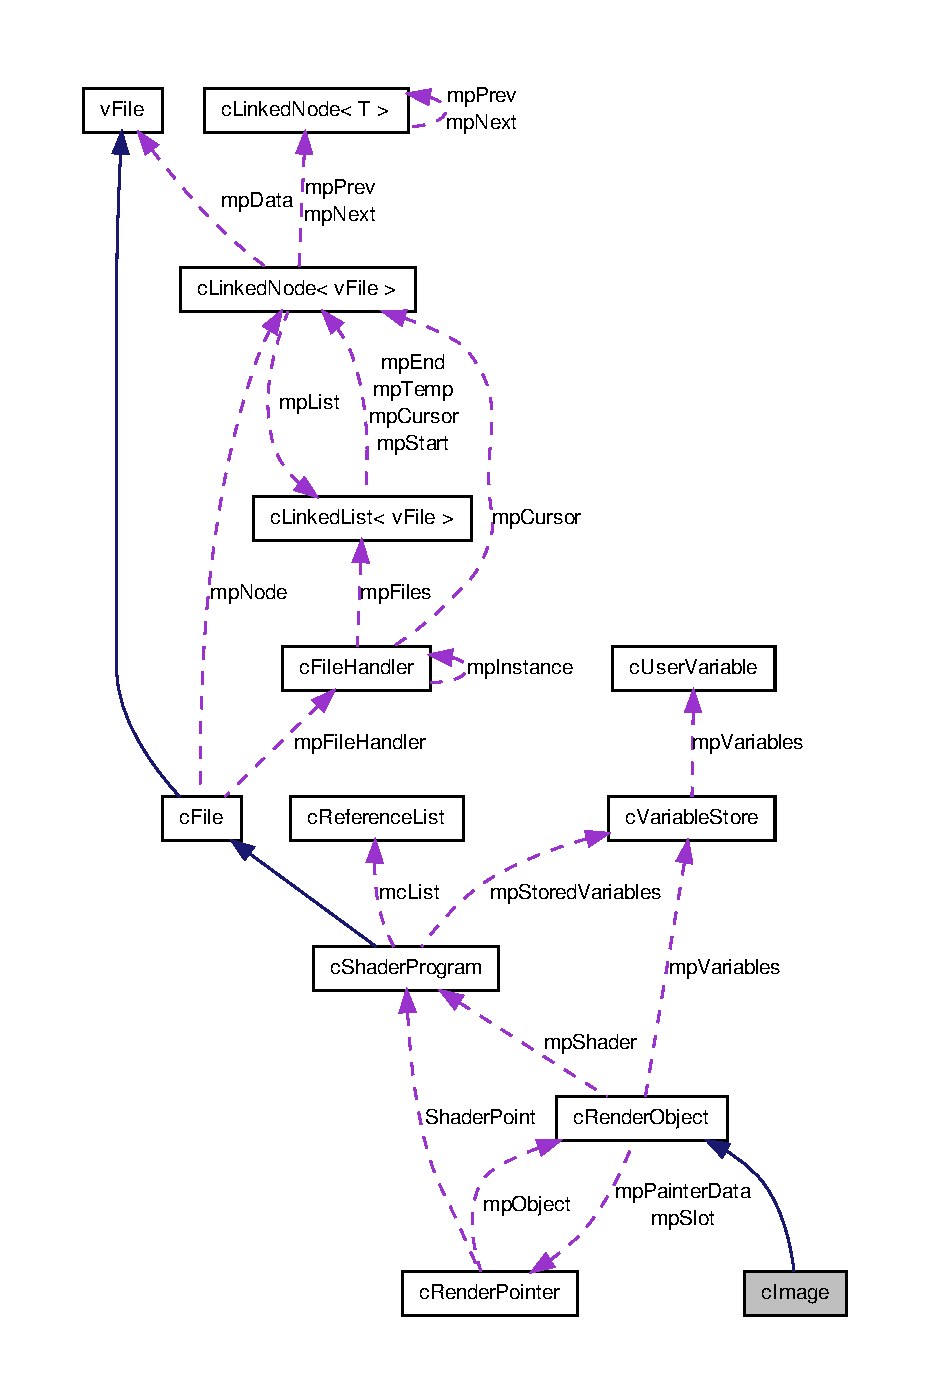
\includegraphics[width=400pt]{classc_image__coll__graph}
\end{center}
\end{figure}
\subsection*{Public Member Functions}
\begin{DoxyCompactItemize}
\item 
\hypertarget{classc_image_a7acf286a86645d8acb39a7b02b06ac0a}{
\hyperlink{classc_image_a7acf286a86645d8acb39a7b02b06ac0a}{cImage} ()}
\label{classc_image_a7acf286a86645d8acb39a7b02b06ac0a}

\begin{DoxyCompactList}\small\item\em Constructor for \hyperlink{classc_image}{cImage}. Will Create an Empty \hyperlink{classc_image}{cImage} Object. \end{DoxyCompactList}\item 
\hypertarget{classc_image_a39864db63ddc349351463e511b7ab433}{
virtual void \hyperlink{classc_image_a39864db63ddc349351463e511b7ab433}{Size} (float lfSize)}
\label{classc_image_a39864db63ddc349351463e511b7ab433}

\begin{DoxyCompactList}\small\item\em Sets the size of the image on screen. Makes the width be lfSize pixels and makes the height to make it appear square. \end{DoxyCompactList}\item 
\hypertarget{classc_image_a3abd5e2a010875c08e08add7e224008e}{
virtual void \hyperlink{classc_image_a3abd5e2a010875c08e08add7e224008e}{Width} (float lfWidth)}
\label{classc_image_a3abd5e2a010875c08e08add7e224008e}

\begin{DoxyCompactList}\small\item\em Sets the size of the image on screen. Makes the width be lfSize pixels and makes the height to make it appear square. \end{DoxyCompactList}\item 
\hypertarget{classc_image_a165ba2ed14e5bf1913357f34ca3a9403}{
virtual void \hyperlink{classc_image_a165ba2ed14e5bf1913357f34ca3a9403}{Height} (float lfHeight)}
\label{classc_image_a165ba2ed14e5bf1913357f34ca3a9403}

\begin{DoxyCompactList}\small\item\em Sets the size of the image on screen. Makes the width be lfSize pixels and makes the height to make it appear square. \end{DoxyCompactList}\item 
\hypertarget{classc_image_aacc1a4884b4fc04b936a1695a393d26a}{
float \hyperlink{classc_image_aacc1a4884b4fc04b936a1695a393d26a}{Width} ()}
\label{classc_image_aacc1a4884b4fc04b936a1695a393d26a}

\begin{DoxyCompactList}\small\item\em Will return the Width of this image in pixels. \end{DoxyCompactList}\item 
\hypertarget{classc_image_adfccfa4a2893b805bf231d5039c27f05}{
float \hyperlink{classc_image_adfccfa4a2893b805bf231d5039c27f05}{Height} ()}
\label{classc_image_adfccfa4a2893b805bf231d5039c27f05}

\begin{DoxyCompactList}\small\item\em Will return the Height of this image in pixels. \end{DoxyCompactList}\end{DoxyCompactItemize}
\subsection*{Friends}
\begin{DoxyCompactItemize}
\item 
\hypertarget{classc_image_ac3e18951e9137b17e506e36253a11cb7}{
class \hyperlink{classc_image_ac3e18951e9137b17e506e36253a11cb7}{cImage3D}}
\label{classc_image_ac3e18951e9137b17e506e36253a11cb7}

\end{DoxyCompactItemize}


\subsection{Detailed Description}
A 2D renderable object. 


\begin{DoxyParams}{Parameters}
{\em lpTexture} & pointer to the texture to bind to this 2D object This is actually a 3D polygon, which has a texture bound to it. it can be used as an OpenGL accelerated sprite. \\
\hline
\end{DoxyParams}

\hypertarget{classc_image3_d}{
\section{cImage3D Class Reference}
\label{classc_image3_d}\index{cImage3D@{cImage3D}}
}


This is a Texture rendered onto a plane, which can be moved as a 3D object. This literally produces a 2D image on a plane in 3D. This can be mvoed like any other object This is good for producing billboards or in game HUDS or screens. Other than specified functions operates in the same way as the class \hyperlink{classc_image}{cImage}. Check the facing of the plane to be sure it displays.  




Collaboration diagram for cImage3D:\nopagebreak
\begin{figure}[H]
\begin{center}
\leavevmode
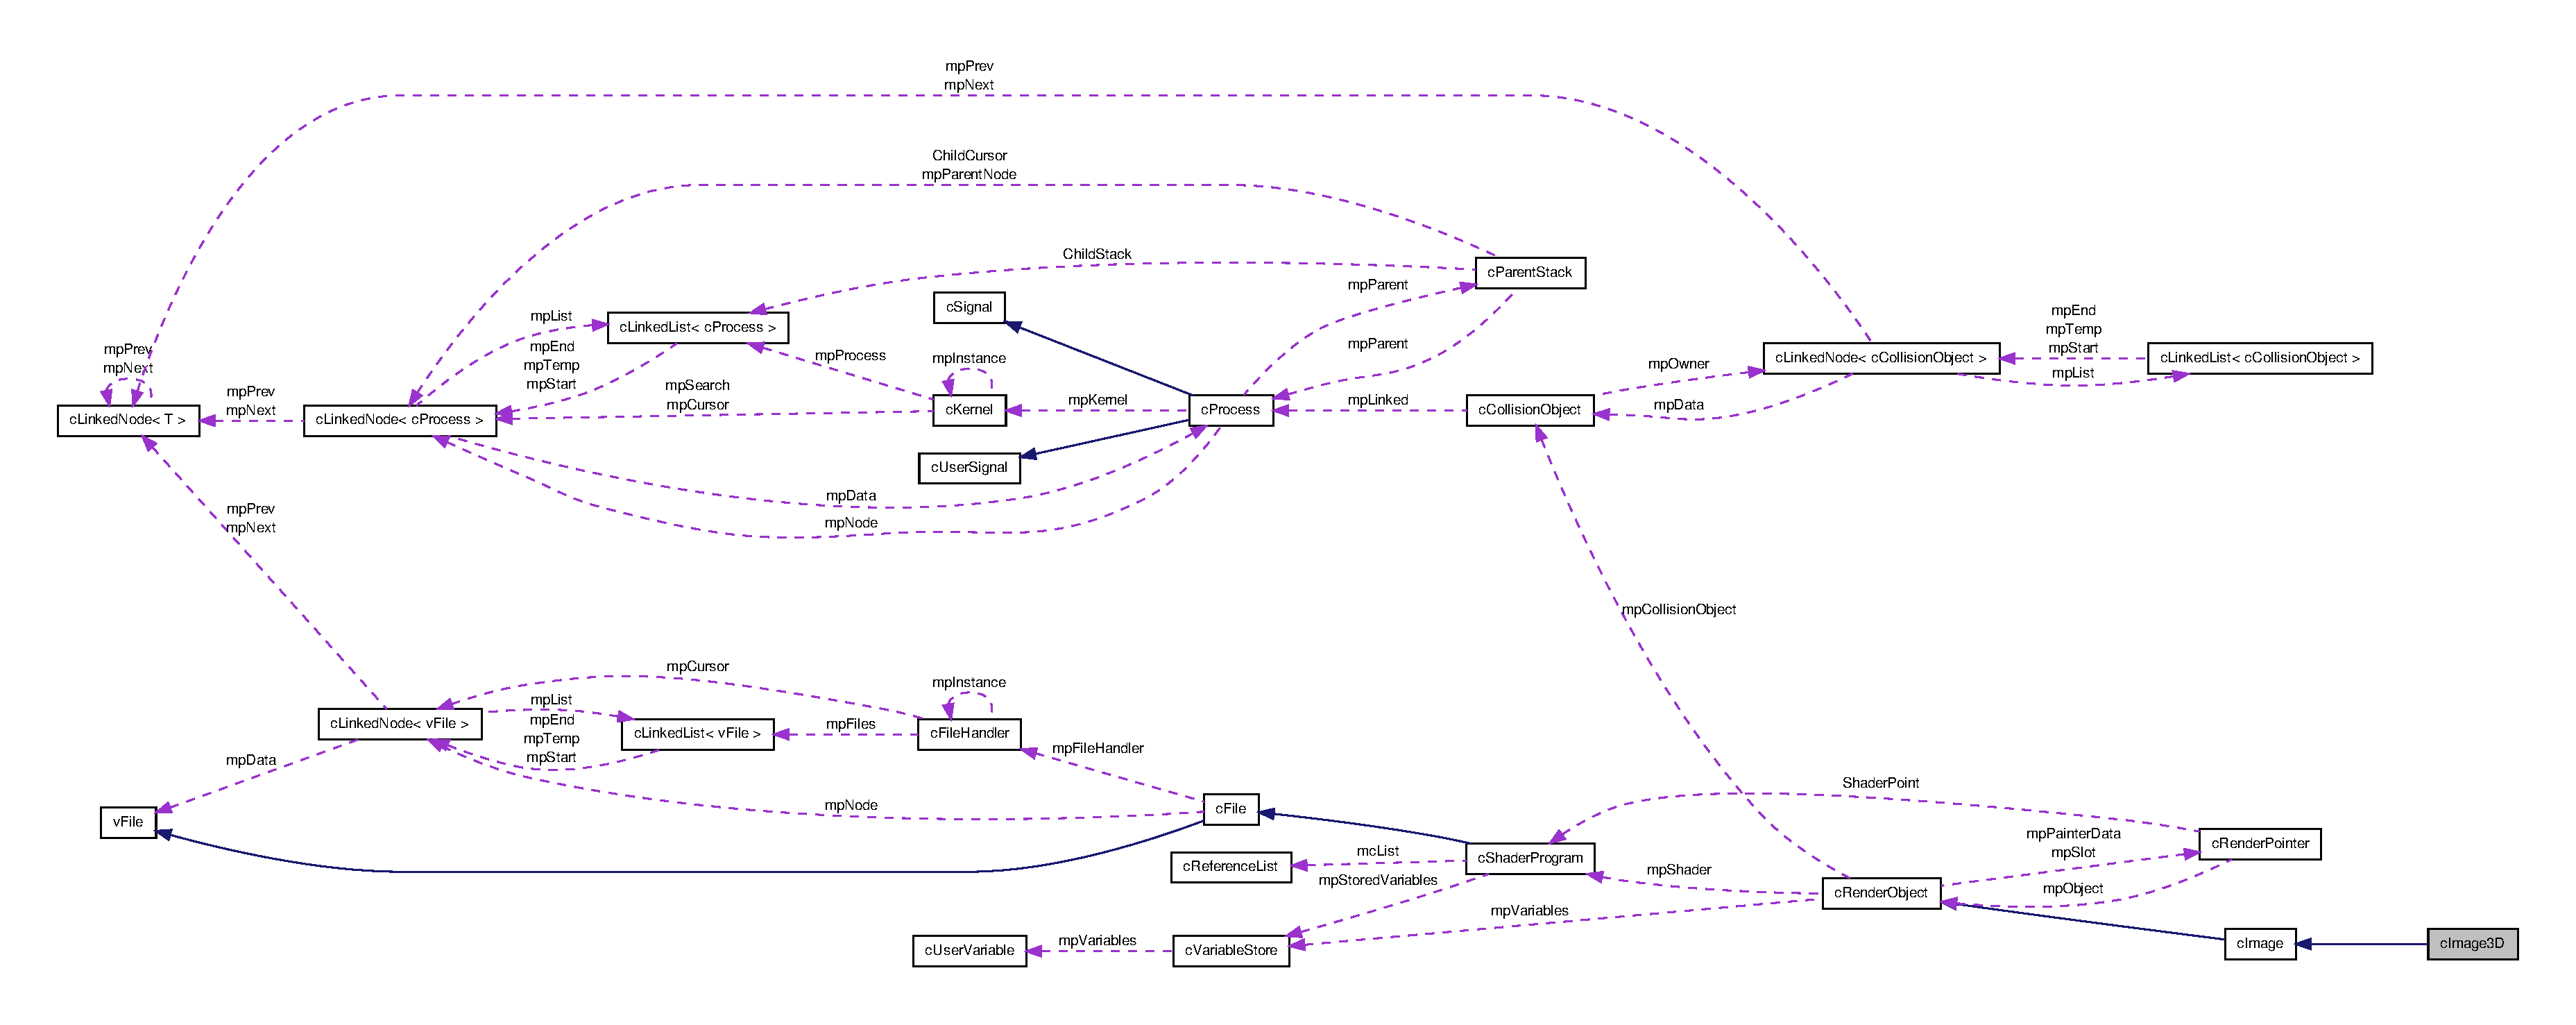
\includegraphics[height=600pt]{classc_image3_d__coll__graph}
\end{center}
\end{figure}


\subsection{Detailed Description}
This is a Texture rendered onto a plane, which can be moved as a 3D object. This literally produces a 2D image on a plane in 3D. This can be mvoed like any other object This is good for producing billboards or in game HUDS or screens. Other than specified functions operates in the same way as the class \hyperlink{classc_image}{cImage}. Check the facing of the plane to be sure it displays. 
\hypertarget{classc_int_attribute_store}{
\section{cIntAttributeStore Class Reference}
\label{classc_int_attribute_store}\index{cIntAttributeStore@{cIntAttributeStore}}
}


More Specific Base class for Attribute Handling classes. Suitable for integer Variables. see \hyperlink{classc_attribute_int_array1}{cAttributeIntArray1}, \hyperlink{classc_attribute_int_array2}{cAttributeIntArray2}, \hyperlink{classc_attribute_int_array3}{cAttributeIntArray3}, \hyperlink{classc_attribute_int_array4}{cAttributeIntArray4}.  




Collaboration diagram for cIntAttributeStore:\nopagebreak
\begin{figure}[H]
\begin{center}
\leavevmode
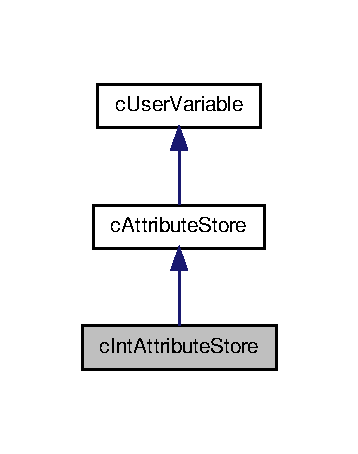
\includegraphics[width=172pt]{classc_int_attribute_store__coll__graph}
\end{center}
\end{figure}
\subsection*{Public Member Functions}
\begin{DoxyCompactItemize}
\item 
\hypertarget{classc_int_attribute_store_a259389363c8795340625fb46de6f1ab0}{
void \hyperlink{classc_int_attribute_store_a259389363c8795340625fb46de6f1ab0}{DataValue} (void $\ast$lpData, uint32 liElements)}
\label{classc_int_attribute_store_a259389363c8795340625fb46de6f1ab0}

\begin{DoxyCompactList}\small\item\em This will Set the Array of Data an Attribute Variable will Use. This will copy the data. It will not automatically update, but the data can be deallocated at any time. \end{DoxyCompactList}\item 
\hypertarget{classc_int_attribute_store_acc2f82fd0dbaab535be958132bf39c6e}{
void \hyperlink{classc_int_attribute_store_acc2f82fd0dbaab535be958132bf39c6e}{DataPointer} (void $\ast$lpData, uint32 liElements)}
\label{classc_int_attribute_store_acc2f82fd0dbaab535be958132bf39c6e}

\begin{DoxyCompactList}\small\item\em This will Set the Array of Data an Attribute Variable will Use. This will not copy the data, but will store a pointer to the data. It will automatically update, but the data passed to it should not be deallocated while the shader is in use. \end{DoxyCompactList}\item 
\hypertarget{classc_int_attribute_store_aecb0e3f10117f4d85e184537a4cc512a}{
void $\ast$ \hyperlink{classc_int_attribute_store_aecb0e3f10117f4d85e184537a4cc512a}{Data} ()}
\label{classc_int_attribute_store_aecb0e3f10117f4d85e184537a4cc512a}

\begin{DoxyCompactList}\small\item\em This will return the data the Function is pointing at. \end{DoxyCompactList}\end{DoxyCompactItemize}


\subsection{Detailed Description}
More Specific Base class for Attribute Handling classes. Suitable for integer Variables. see \hyperlink{classc_attribute_int_array1}{cAttributeIntArray1}, \hyperlink{classc_attribute_int_array2}{cAttributeIntArray2}, \hyperlink{classc_attribute_int_array3}{cAttributeIntArray3}, \hyperlink{classc_attribute_int_array4}{cAttributeIntArray4}. 
\hypertarget{classc_int_uniform_store}{
\section{cIntUniformStore Class Reference}
\label{classc_int_uniform_store}\index{cIntUniformStore@{cIntUniformStore}}
}


More Specific Base class for Uniform Handling classes. Suitable for Integer Variables. see \hyperlink{classc_uniform_int_vector1}{cUniformIntVector1}, \hyperlink{classc_uniform_int_vector2}{cUniformIntVector2}, \hyperlink{classc_uniform_int_vector3}{cUniformIntVector3}, \hyperlink{classc_uniform_int_vector4}{cUniformIntVector4}.  




Collaboration diagram for cIntUniformStore:\nopagebreak
\begin{figure}[H]
\begin{center}
\leavevmode
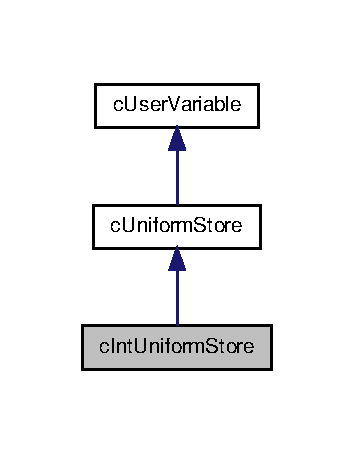
\includegraphics[width=170pt]{classc_int_uniform_store__coll__graph}
\end{center}
\end{figure}
\subsection*{Public Member Functions}
\begin{DoxyCompactItemize}
\item 
\hypertarget{classc_int_uniform_store_a1a55824498ebea1af11f4e89c8868e77}{
void \hyperlink{classc_int_uniform_store_a1a55824498ebea1af11f4e89c8868e77}{DataPointer} (void $\ast$lpData)}
\label{classc_int_uniform_store_a1a55824498ebea1af11f4e89c8868e77}

\begin{DoxyCompactList}\small\item\em This will Set the Data a Uniform Variable will Use. This will not copy the data, but will store a pointer to the data. It will automatically update, but the data passed to it should not be deallocated while the shader is in use. \end{DoxyCompactList}\item 
\hypertarget{classc_int_uniform_store_aac23b6807a6fec5f9f723cedd8b3457b}{
void $\ast$ \hyperlink{classc_int_uniform_store_aac23b6807a6fec5f9f723cedd8b3457b}{Data} ()}
\label{classc_int_uniform_store_aac23b6807a6fec5f9f723cedd8b3457b}

\begin{DoxyCompactList}\small\item\em This will return the data the Function is pointing at. \end{DoxyCompactList}\end{DoxyCompactItemize}


\subsection{Detailed Description}
More Specific Base class for Uniform Handling classes. Suitable for Integer Variables. see \hyperlink{classc_uniform_int_vector1}{cUniformIntVector1}, \hyperlink{classc_uniform_int_vector2}{cUniformIntVector2}, \hyperlink{classc_uniform_int_vector3}{cUniformIntVector3}, \hyperlink{classc_uniform_int_vector4}{cUniformIntVector4}. 
\hypertarget{classc_kernel}{
\section{cKernel Class Reference}
\label{classc_kernel}\index{cKernel@{cKernel}}
}


Kernel Object. Handles Processes. Tracks, runs and deletes current processes. Has complete control over every \hyperlink{classc_process}{cProcess} object. Will run all awake alive processes every process cycle, will delete dead processes. Also controls the activation of rendering frames and handling interactions with the operating system.  




Collaboration diagram for cKernel:
\nopagebreak
\begin{figure}[H]
\begin{center}
\leavevmode
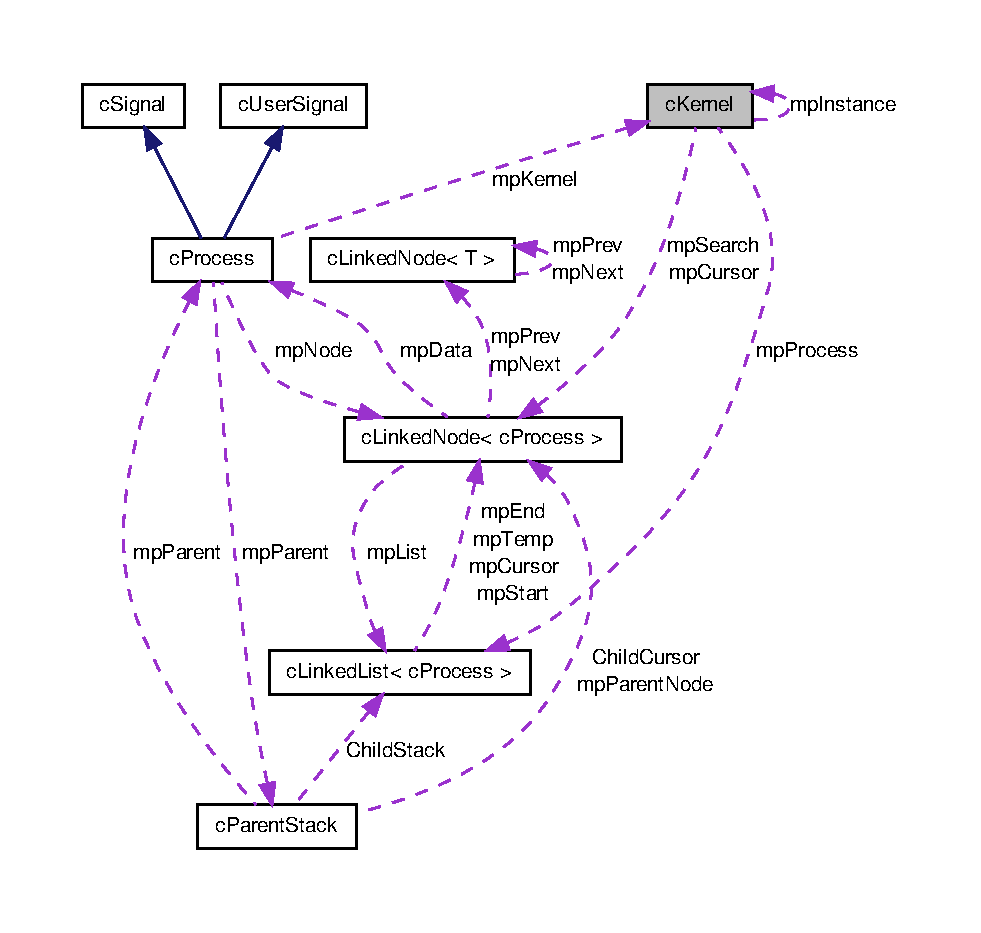
\includegraphics[width=400pt]{classc_kernel__coll__graph}
\end{center}
\end{figure}
\subsection*{Public Member Functions}
\begin{DoxyCompactItemize}
\item 
void \hyperlink{classc_kernel_a721f5ad665c512b511ff8d344010385e}{KillProgram} ()
\begin{DoxyCompactList}\small\item\em Will kill the entire program. Will delete every process and then exit. \item\end{DoxyCompactList}\item 
\hyperlink{classc_kernel_aa17d85bb9118c9de59fe0c6301301a39}{$\sim$cKernel} ()
\item 
void \hyperlink{classc_kernel_afbbf3ca5d7f5db9c91f1c279c0109b2f}{Update} ()
\item 
\hyperlink{classc_linked_node}{cLinkedNode}$<$ \hyperlink{classv_process}{vProcess} $>$ $\ast$ \hyperlink{classc_kernel_a4ec4faedede9de3cae4fc5fbc4469a1b}{Add} (\hyperlink{classv_process}{vProcess} $\ast$lpNew)
\item 
void \hyperlink{classc_kernel_a59c9a956e6a6666a57c2d85e463381d8}{Remove} (\hyperlink{classc_linked_node}{cLinkedNode}$<$ \hyperlink{classv_process}{vProcess} $>$ $\ast$lpOld)
\item 
void \hyperlink{classc_kernel_af4c3e32a55fdef58236378eed46afdfe}{DeleteAll} ()
\begin{DoxyCompactList}\small\item\em Will Delete all the processes in the current process list. This will effectively end the program. \item\end{DoxyCompactList}\item 
{\footnotesize template$<$class tType $>$ }\\tType $\ast$ \hyperlink{classc_kernel_a56083c090177a8a2a9bb50ad58e712c3}{FindProcess} ()
\begin{DoxyCompactList}\small\item\em This Function will search for a process of either tType OR a type which has uses the type tType as a base type. \item\end{DoxyCompactList}\item 
void \hyperlink{classc_kernel_a42d5d224af7acfe4aee27b7cee2b0a02}{ResetFindProcess} ()
\begin{DoxyCompactList}\small\item\em This Function will reset \hyperlink{classc_kernel_a56083c090177a8a2a9bb50ad58e712c3}{FindProcess()} to search from the start of the process List. \item\end{DoxyCompactList}\end{DoxyCompactItemize}
\subsection*{Static Public Member Functions}
\begin{DoxyCompactItemize}
\item 
static \hyperlink{classc_kernel}{cKernel} $\ast$ \hyperlink{classc_kernel_a5bd65ef494632b9fd585a6f6cae375e7}{Instance} ()
\begin{DoxyCompactList}\small\item\em Function which returns current Kernel Instance. Will Create a new instance if one does not already exist. \item\end{DoxyCompactList}\end{DoxyCompactItemize}


\subsection{Detailed Description}
Kernel Object. Handles Processes. Tracks, runs and deletes current processes. Has complete control over every \hyperlink{classc_process}{cProcess} object. Will run all awake alive processes every process cycle, will delete dead processes. Also controls the activation of rendering frames and handling interactions with the operating system. 

Definition at line 15 of file WTKernel.h.



\subsection{Constructor \& Destructor Documentation}
\hypertarget{classc_kernel_aa17d85bb9118c9de59fe0c6301301a39}{
\index{cKernel@{cKernel}!$\sim$cKernel@{$\sim$cKernel}}
\index{$\sim$cKernel@{$\sim$cKernel}!cKernel@{cKernel}}
\subsubsection[{$\sim$cKernel}]{\setlength{\rightskip}{0pt plus 5cm}cKernel::$\sim$cKernel (
\begin{DoxyParamCaption}
{}
\end{DoxyParamCaption}
)}}
\label{classc_kernel_aa17d85bb9118c9de59fe0c6301301a39}


Definition at line 94 of file WTKernel.cpp.



\subsection{Member Function Documentation}
\hypertarget{classc_kernel_a4ec4faedede9de3cae4fc5fbc4469a1b}{
\index{cKernel@{cKernel}!Add@{Add}}
\index{Add@{Add}!cKernel@{cKernel}}
\subsubsection[{Add}]{\setlength{\rightskip}{0pt plus 5cm}{\bf cLinkedNode}$<$ {\bf vProcess} $>$ $\ast$ cKernel::Add (
\begin{DoxyParamCaption}
\item[{{\bf vProcess} $\ast$}]{lpNew}
\end{DoxyParamCaption}
)}}
\label{classc_kernel_a4ec4faedede9de3cae4fc5fbc4469a1b}


Definition at line 123 of file WTKernel.cpp.

\hypertarget{classc_kernel_af4c3e32a55fdef58236378eed46afdfe}{
\index{cKernel@{cKernel}!DeleteAll@{DeleteAll}}
\index{DeleteAll@{DeleteAll}!cKernel@{cKernel}}
\subsubsection[{DeleteAll}]{\setlength{\rightskip}{0pt plus 5cm}void cKernel::DeleteAll (
\begin{DoxyParamCaption}
{}
\end{DoxyParamCaption}
)}}
\label{classc_kernel_af4c3e32a55fdef58236378eed46afdfe}


Will Delete all the processes in the current process list. This will effectively end the program. 



Definition at line 12 of file WTKernel.cpp.

\hypertarget{classc_kernel_a56083c090177a8a2a9bb50ad58e712c3}{
\index{cKernel@{cKernel}!FindProcess@{FindProcess}}
\index{FindProcess@{FindProcess}!cKernel@{cKernel}}
\subsubsection[{FindProcess}]{\setlength{\rightskip}{0pt plus 5cm}template$<$class tType $>$ tType $\ast$ cKernel::FindProcess (
\begin{DoxyParamCaption}
{}
\end{DoxyParamCaption}
)}}
\label{classc_kernel_a56083c090177a8a2a9bb50ad58e712c3}


This Function will search for a process of either tType OR a type which has uses the type tType as a base type. 


\begin{DoxyParams}{Parameters}
{\em mpType} & is a pointer of the type (or base type) of the desired process. \\
\hline
\end{DoxyParams}
\begin{DoxyReturn}{Returns}
Will return a pointer to a process currently in the process list of the correct type.
\end{DoxyReturn}
This Function takes the type of the pointer handed to the function and will search for a process which is of type tType or inherits tType. Can be used to find processes of a certain type or genus. Each call of this function will continue searching from the position stored in mpSearch. Between searches for processes of different types use the function \hyperlink{classc_kernel_a42d5d224af7acfe4aee27b7cee2b0a02}{ResetFindProcess()}. 
\begin{DoxyCode}
        cGunShip *mpGunShip;
        cBattleShip *mpBattleShip;

        mpGunShip = FindProcess(mpGunShip);
        ResetFindProcess();
        mpBattleShip = FindProcess(mpBattleShip);
\end{DoxyCode}
 

Definition at line 92 of file WTKernel.h.

\hypertarget{classc_kernel_a5bd65ef494632b9fd585a6f6cae375e7}{
\index{cKernel@{cKernel}!Instance@{Instance}}
\index{Instance@{Instance}!cKernel@{cKernel}}
\subsubsection[{Instance}]{\setlength{\rightskip}{0pt plus 5cm}{\bf cKernel} $\ast$ cKernel::Instance (
\begin{DoxyParamCaption}
{}
\end{DoxyParamCaption}
)\hspace{0.3cm}{\ttfamily  \mbox{[}static\mbox{]}}}}
\label{classc_kernel_a5bd65ef494632b9fd585a6f6cae375e7}


Function which returns current Kernel Instance. Will Create a new instance if one does not already exist. 



Definition at line 139 of file WTKernel.cpp.

\hypertarget{classc_kernel_a721f5ad665c512b511ff8d344010385e}{
\index{cKernel@{cKernel}!KillProgram@{KillProgram}}
\index{KillProgram@{KillProgram}!cKernel@{cKernel}}
\subsubsection[{KillProgram}]{\setlength{\rightskip}{0pt plus 5cm}void cKernel::KillProgram (
\begin{DoxyParamCaption}
{}
\end{DoxyParamCaption}
)}}
\label{classc_kernel_a721f5ad665c512b511ff8d344010385e}


Will kill the entire program. Will delete every process and then exit. 



Definition at line 162 of file WTKernel.cpp.

\hypertarget{classc_kernel_a59c9a956e6a6666a57c2d85e463381d8}{
\index{cKernel@{cKernel}!Remove@{Remove}}
\index{Remove@{Remove}!cKernel@{cKernel}}
\subsubsection[{Remove}]{\setlength{\rightskip}{0pt plus 5cm}void cKernel::Remove (
\begin{DoxyParamCaption}
\item[{{\bf cLinkedNode}$<$ {\bf vProcess} $>$ $\ast$}]{lpOld}
\end{DoxyParamCaption}
)}}
\label{classc_kernel_a59c9a956e6a6666a57c2d85e463381d8}


Definition at line 134 of file WTKernel.cpp.

\hypertarget{classc_kernel_a42d5d224af7acfe4aee27b7cee2b0a02}{
\index{cKernel@{cKernel}!ResetFindProcess@{ResetFindProcess}}
\index{ResetFindProcess@{ResetFindProcess}!cKernel@{cKernel}}
\subsubsection[{ResetFindProcess}]{\setlength{\rightskip}{0pt plus 5cm}void cKernel::ResetFindProcess (
\begin{DoxyParamCaption}
{}
\end{DoxyParamCaption}
)}}
\label{classc_kernel_a42d5d224af7acfe4aee27b7cee2b0a02}


This Function will reset \hyperlink{classc_kernel_a56083c090177a8a2a9bb50ad58e712c3}{FindProcess()} to search from the start of the process List. 



Definition at line 160 of file WTKernel.cpp.

\hypertarget{classc_kernel_afbbf3ca5d7f5db9c91f1c279c0109b2f}{
\index{cKernel@{cKernel}!Update@{Update}}
\index{Update@{Update}!cKernel@{cKernel}}
\subsubsection[{Update}]{\setlength{\rightskip}{0pt plus 5cm}void cKernel::Update (
\begin{DoxyParamCaption}
{}
\end{DoxyParamCaption}
)}}
\label{classc_kernel_afbbf3ca5d7f5db9c91f1c279c0109b2f}


Definition at line 18 of file WTKernel.cpp.


\hypertarget{classc_key_store}{
\section{cKeyStore Class Reference}
\label{classc_key_store}\index{cKeyStore@{cKeyStore}}
}


This class stores all the input data for a single keyboard.  


\subsection*{Public Member Functions}
\begin{DoxyCompactItemize}
\item 
\hypertarget{classc_key_store_a338766086dd09a48b8cefd33fb35bc7a}{
\hyperlink{classc_key_store_a338766086dd09a48b8cefd33fb35bc7a}{cKeyStore} ()}
\label{classc_key_store_a338766086dd09a48b8cefd33fb35bc7a}

\begin{DoxyCompactList}\small\item\em This will return a specific key state, using the relevant key code. \end{DoxyCompactList}\end{DoxyCompactItemize}
\subsection*{Public Attributes}
\begin{DoxyCompactItemize}
\item 
\hypertarget{classc_key_store_a1b0760ec36eafb3c3ef74b21e60e4009}{
bool \hyperlink{classc_key_store_a1b0760ec36eafb3c3ef74b21e60e4009}{key} \mbox{[}2\mbox{]}\mbox{[}256\mbox{]}}
\label{classc_key_store_a1b0760ec36eafb3c3ef74b21e60e4009}

\begin{DoxyCompactList}\small\item\em This is the array of keystates. \end{DoxyCompactList}\end{DoxyCompactItemize}


\subsection{Detailed Description}
This class stores all the input data for a single keyboard. 
\hypertarget{classc_landscape}{
\section{cLandscape Class Reference}
\label{classc_landscape}\index{cLandscape@{cLandscape}}
}


A height map based, matrix structured Landscape. Landscape is composed of a matrix of square polygons. The heights of each vertex is produced using the packaging software, and is generated from a bitmap.  




Collaboration diagram for cLandscape:\nopagebreak
\begin{figure}[H]
\begin{center}
\leavevmode
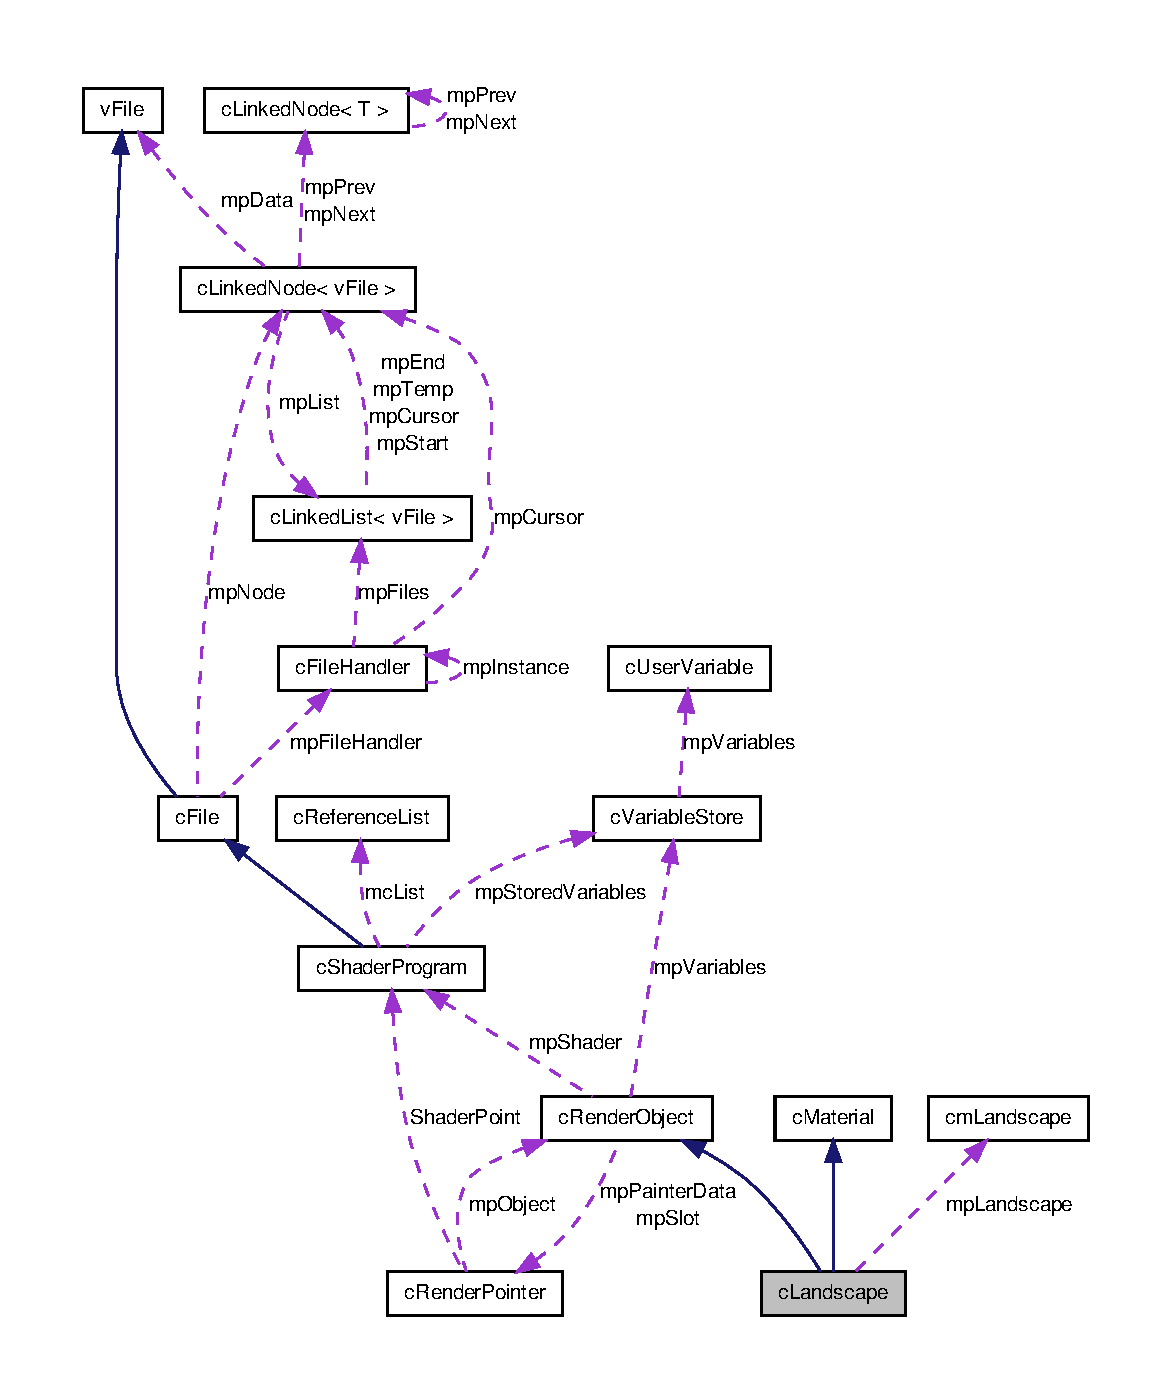
\includegraphics[width=400pt]{classc_landscape__coll__graph}
\end{center}
\end{figure}
\subsection*{Public Member Functions}
\begin{DoxyCompactItemize}
\item 
\hypertarget{classc_landscape_afc86bc9f2d3ce929abc8ef5e6dcd1248}{
\hyperlink{classc_landscape_afc86bc9f2d3ce929abc8ef5e6dcd1248}{cLandscape} (\hyperlink{classcm_landscape}{cmLandscape} $\ast$lpModel, \hyperlink{classc_camera}{cCamera} $\ast$lpCamera)}
\label{classc_landscape_afc86bc9f2d3ce929abc8ef5e6dcd1248}

\begin{DoxyCompactList}\small\item\em Create a landscape object and set its height map and texture. Can also assign the Landscape to a Camera. \end{DoxyCompactList}\item 
\hypertarget{classc_landscape_a1fa3ad374cf96116beb5791cc9aa713e}{
\hyperlink{classc_landscape_a1fa3ad374cf96116beb5791cc9aa713e}{cLandscape} (\hyperlink{classcm_landscape}{cmLandscape} $\ast$lpModel=0)}
\label{classc_landscape_a1fa3ad374cf96116beb5791cc9aa713e}

\begin{DoxyCompactList}\small\item\em Create a landscape object and set its height map and texture. \end{DoxyCompactList}\item 
\hypertarget{classc_landscape_ac945c88a536fee7dd2f499e199225939}{
void \hyperlink{classc_landscape_ac945c88a536fee7dd2f499e199225939}{Landscape} (\hyperlink{classcm_landscape}{cmLandscape} $\ast$lpLandscape)}
\label{classc_landscape_ac945c88a536fee7dd2f499e199225939}

\begin{DoxyCompactList}\small\item\em Set the current height map for this landscape object. \end{DoxyCompactList}\item 
\hypertarget{classc_landscape_ae30d44a1e780ef4f120c4aa4dc460c06}{
void \hyperlink{classc_landscape_ae30d44a1e780ef4f120c4aa4dc460c06}{Landscape} (string lsLandscape)}
\label{classc_landscape_ae30d44a1e780ef4f120c4aa4dc460c06}

\begin{DoxyCompactList}\small\item\em Set the current height map for this landscape object to use. \end{DoxyCompactList}\item 
\hypertarget{classc_landscape_a36f6a35064d14d460f99464181c5c830}{
float \hyperlink{classc_landscape_a36f6a35064d14d460f99464181c5c830}{GetHeight} (float lfX, float lfZ)}
\label{classc_landscape_a36f6a35064d14d460f99464181c5c830}

\begin{DoxyCompactList}\small\item\em Will return the height at Global co-\/ordinates lfX,lfZ. \end{DoxyCompactList}\item 
\hypertarget{classc_landscape_acdb3f590236a85b1423acc47f064e9b7}{
float \hyperlink{classc_landscape_acdb3f590236a85b1423acc47f064e9b7}{GetHeightLocal} (float lfX, float lfZ)}
\label{classc_landscape_acdb3f590236a85b1423acc47f064e9b7}

\begin{DoxyCompactList}\small\item\em Will return the height at the Local position lfX,lfZ (relative to landscapes corner) \end{DoxyCompactList}\item 
\hypertarget{classc_landscape_a7642e8b5062010778a1ad8913077a661}{
float \hyperlink{classc_landscape_a7642e8b5062010778a1ad8913077a661}{GetVertexHeight} (int liX, int liZ)}
\label{classc_landscape_a7642e8b5062010778a1ad8913077a661}

\begin{DoxyCompactList}\small\item\em Will return the height of the vertex at liX,liZ. (position is based on number of segments NOT distance) \end{DoxyCompactList}\end{DoxyCompactItemize}


\subsection{Detailed Description}
A height map based, matrix structured Landscape. Landscape is composed of a matrix of square polygons. The heights of each vertex is produced using the packaging software, and is generated from a bitmap. 
\hypertarget{classc_landscape_mesh_file}{
\section{cLandscapeMeshFile Class Reference}
\label{classc_landscape_mesh_file}\index{cLandscapeMeshFile@{cLandscapeMeshFile}}
}


This is the class which the Landscape File is stored in. This can be passed to any of \hyperlink{classcm_landscape}{cmLandscape}, cLandscapeMeshIndividual or cLandscapeMeshRandom.  




Collaboration diagram for cLandscapeMeshFile:\nopagebreak
\begin{figure}[H]
\begin{center}
\leavevmode
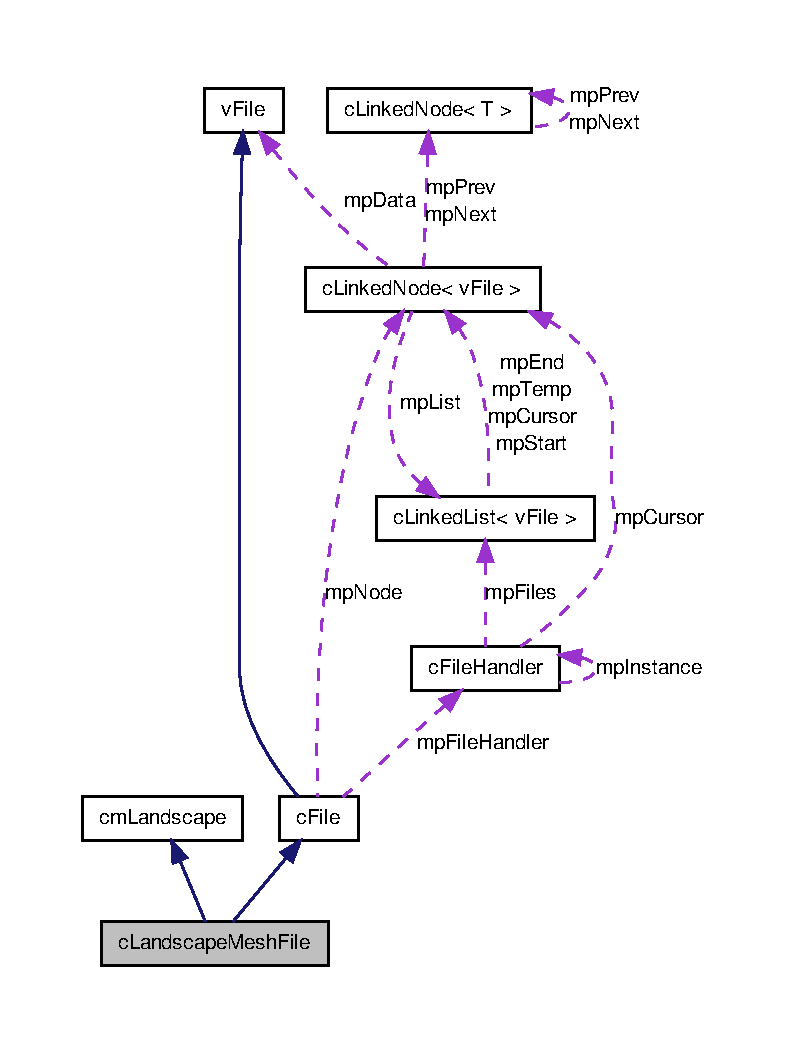
\includegraphics[width=378pt]{classc_landscape_mesh_file__coll__graph}
\end{center}
\end{figure}
\subsection*{Friends}
\begin{DoxyCompactItemize}
\item 
\hypertarget{classc_landscape_mesh_file_a642b5e78056302f99f656983a53beb6d}{
class \hyperlink{classc_landscape_mesh_file_a642b5e78056302f99f656983a53beb6d}{cmLandscape}}
\label{classc_landscape_mesh_file_a642b5e78056302f99f656983a53beb6d}

\end{DoxyCompactItemize}


\subsection{Detailed Description}
This is the class which the Landscape File is stored in. This can be passed to any of \hyperlink{classcm_landscape}{cmLandscape}, cLandscapeMeshIndividual or cLandscapeMeshRandom. 
\hypertarget{classc_light_handler}{
\section{cLightHandler Class Reference}
\label{classc_light_handler}\index{cLightHandler@{cLightHandler}}
}


\hyperlink{classc_light_handler}{cLightHandler} will control the OpenGL Lights. It will turn off lights not required or possible for different renderings to increase speed and circumvent the OpenGL limit of active lights. OpenGL has a limited number of lights that can be used at any one time. This handler identifies the lights which will have the greatest effect on the current object and prepares the optimal selection of lights for rendering the scene.  




Collaboration diagram for cLightHandler:
\nopagebreak
\begin{figure}[H]
\begin{center}
\leavevmode
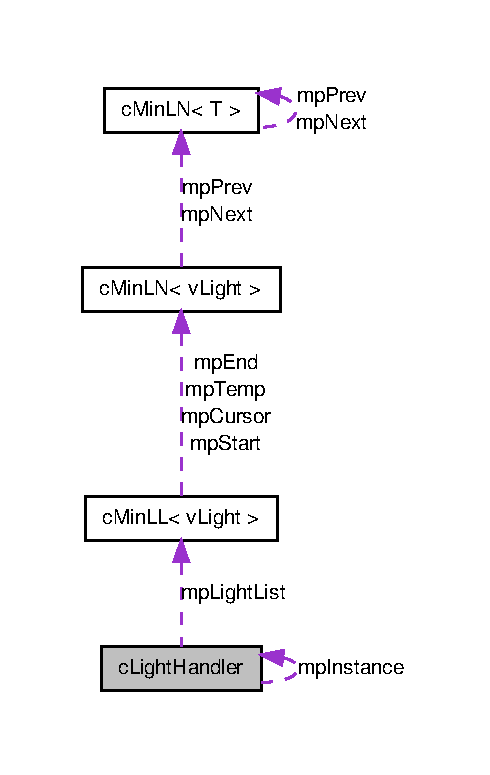
\includegraphics[width=317pt]{classc_light_handler__coll__graph}
\end{center}
\end{figure}
\subsection*{Public Member Functions}
\begin{DoxyCompactItemize}
\item 
\hyperlink{classc_light_handler_a17ed4af735943e71d486ebbe15b70eb8}{$\sim$cLightHandler} ()
\item 
\hyperlink{classc_min_l_n}{cMinLN}$<$ \hyperlink{classv_light}{vLight} $>$ $\ast$ \hyperlink{classc_light_handler_ad11b0b020fe2dbe57e0cdff69e4ccdbe}{Add} (\hyperlink{classv_light}{vLight} $\ast$lpNew)
\item 
void \hyperlink{classc_light_handler_a6961b97a431244a4494e36fe468b67fb}{PrepareLight} ()
\begin{DoxyCompactList}\small\item\em Will Prepare all the Lights for Rendering generally. \item\end{DoxyCompactList}\item 
void \hyperlink{classc_light_handler_af496ab1e05b26dcc1ae5da53a84da271}{PrepareLight} (\hyperlink{classc_matrix4}{cMatrix4} $\ast$mpObj)
\begin{DoxyCompactList}\small\item\em Will Prepare the Lights for Rendering a specific Object. \item\end{DoxyCompactList}\item 
void \hyperlink{classc_light_handler_a8c89de26ed57dca05e0daa5dbf089f8f}{Remove} (\hyperlink{classc_min_l_n}{cMinLN}$<$ \hyperlink{classv_light}{vLight} $>$ $\ast$lpOld)
\item 
void \hyperlink{classc_light_handler_aa3fa6f26deaa89361a703e94224bf641}{DeleteAll} ()
\begin{DoxyCompactList}\small\item\em Will Delete all the processes in the current Light list. \item\end{DoxyCompactList}\end{DoxyCompactItemize}
\subsection*{Static Public Member Functions}
\begin{DoxyCompactItemize}
\item 
static void \hyperlink{classc_light_handler_ac1357d0e2b0a15413a5a6b16e1b3abab}{SetupLights} ()
\item 
static \hyperlink{classc_light_handler}{cLightHandler} $\ast$ \hyperlink{classc_light_handler_ac0473959c255734fa3937f3d09e718a0}{Instance} ()
\begin{DoxyCompactList}\small\item\em This function will return a pointer to the current \hyperlink{classc_light_handler}{cLightHandler} Object. \item\end{DoxyCompactList}\end{DoxyCompactItemize}


\subsection{Detailed Description}
\hyperlink{classc_light_handler}{cLightHandler} will control the OpenGL Lights. It will turn off lights not required or possible for different renderings to increase speed and circumvent the OpenGL limit of active lights. OpenGL has a limited number of lights that can be used at any one time. This handler identifies the lights which will have the greatest effect on the current object and prepares the optimal selection of lights for rendering the scene. 

Definition at line 15 of file WTcLightHandler.h.



\subsection{Constructor \& Destructor Documentation}
\hypertarget{classc_light_handler_a17ed4af735943e71d486ebbe15b70eb8}{
\index{cLightHandler@{cLightHandler}!$\sim$cLightHandler@{$\sim$cLightHandler}}
\index{$\sim$cLightHandler@{$\sim$cLightHandler}!cLightHandler@{cLightHandler}}
\subsubsection[{$\sim$cLightHandler}]{\setlength{\rightskip}{0pt plus 5cm}cLightHandler::$\sim$cLightHandler (
\begin{DoxyParamCaption}
{}
\end{DoxyParamCaption}
)}}
\label{classc_light_handler_a17ed4af735943e71d486ebbe15b70eb8}


Definition at line 9 of file WTcLightHandler.cpp.



\subsection{Member Function Documentation}
\hypertarget{classc_light_handler_ad11b0b020fe2dbe57e0cdff69e4ccdbe}{
\index{cLightHandler@{cLightHandler}!Add@{Add}}
\index{Add@{Add}!cLightHandler@{cLightHandler}}
\subsubsection[{Add}]{\setlength{\rightskip}{0pt plus 5cm}{\bf cMinLN}$<$ {\bf vLight} $>$ $\ast$ cLightHandler::Add (
\begin{DoxyParamCaption}
\item[{{\bf vLight} $\ast$}]{lpNew}
\end{DoxyParamCaption}
)}}
\label{classc_light_handler_ad11b0b020fe2dbe57e0cdff69e4ccdbe}


Definition at line 36 of file WTcLightHandler.cpp.

\hypertarget{classc_light_handler_aa3fa6f26deaa89361a703e94224bf641}{
\index{cLightHandler@{cLightHandler}!DeleteAll@{DeleteAll}}
\index{DeleteAll@{DeleteAll}!cLightHandler@{cLightHandler}}
\subsubsection[{DeleteAll}]{\setlength{\rightskip}{0pt plus 5cm}void cLightHandler::DeleteAll (
\begin{DoxyParamCaption}
{}
\end{DoxyParamCaption}
)}}
\label{classc_light_handler_aa3fa6f26deaa89361a703e94224bf641}


Will Delete all the processes in the current Light list. 



Definition at line 50 of file WTcLightHandler.cpp.

\hypertarget{classc_light_handler_ac0473959c255734fa3937f3d09e718a0}{
\index{cLightHandler@{cLightHandler}!Instance@{Instance}}
\index{Instance@{Instance}!cLightHandler@{cLightHandler}}
\subsubsection[{Instance}]{\setlength{\rightskip}{0pt plus 5cm}{\bf cLightHandler} $\ast$ cLightHandler::Instance (
\begin{DoxyParamCaption}
{}
\end{DoxyParamCaption}
)\hspace{0.3cm}{\ttfamily  \mbox{[}static\mbox{]}}}}
\label{classc_light_handler_ac0473959c255734fa3937f3d09e718a0}


This function will return a pointer to the current \hyperlink{classc_light_handler}{cLightHandler} Object. 



Definition at line 18 of file WTcLightHandler.cpp.

\hypertarget{classc_light_handler_af496ab1e05b26dcc1ae5da53a84da271}{
\index{cLightHandler@{cLightHandler}!PrepareLight@{PrepareLight}}
\index{PrepareLight@{PrepareLight}!cLightHandler@{cLightHandler}}
\subsubsection[{PrepareLight}]{\setlength{\rightskip}{0pt plus 5cm}void cLightHandler::PrepareLight (
\begin{DoxyParamCaption}
\item[{{\bf cMatrix4} $\ast$}]{mpObj}
\end{DoxyParamCaption}
)}}
\label{classc_light_handler_af496ab1e05b26dcc1ae5da53a84da271}


Will Prepare the Lights for Rendering a specific Object. 



Definition at line 72 of file WTcLightHandler.cpp.

\hypertarget{classc_light_handler_a6961b97a431244a4494e36fe468b67fb}{
\index{cLightHandler@{cLightHandler}!PrepareLight@{PrepareLight}}
\index{PrepareLight@{PrepareLight}!cLightHandler@{cLightHandler}}
\subsubsection[{PrepareLight}]{\setlength{\rightskip}{0pt plus 5cm}void cLightHandler::PrepareLight (
\begin{DoxyParamCaption}
{}
\end{DoxyParamCaption}
)}}
\label{classc_light_handler_a6961b97a431244a4494e36fe468b67fb}


Will Prepare all the Lights for Rendering generally. 



Definition at line 61 of file WTcLightHandler.cpp.

\hypertarget{classc_light_handler_a8c89de26ed57dca05e0daa5dbf089f8f}{
\index{cLightHandler@{cLightHandler}!Remove@{Remove}}
\index{Remove@{Remove}!cLightHandler@{cLightHandler}}
\subsubsection[{Remove}]{\setlength{\rightskip}{0pt plus 5cm}void cLightHandler::Remove (
\begin{DoxyParamCaption}
\item[{{\bf cMinLN}$<$ {\bf vLight} $>$ $\ast$}]{lpOld}
\end{DoxyParamCaption}
)}}
\label{classc_light_handler_a8c89de26ed57dca05e0daa5dbf089f8f}


Definition at line 56 of file WTcLightHandler.cpp.

\hypertarget{classc_light_handler_ac1357d0e2b0a15413a5a6b16e1b3abab}{
\index{cLightHandler@{cLightHandler}!SetupLights@{SetupLights}}
\index{SetupLights@{SetupLights}!cLightHandler@{cLightHandler}}
\subsubsection[{SetupLights}]{\setlength{\rightskip}{0pt plus 5cm}void cLightHandler::SetupLights (
\begin{DoxyParamCaption}
{}
\end{DoxyParamCaption}
)\hspace{0.3cm}{\ttfamily  \mbox{[}static\mbox{]}}}}
\label{classc_light_handler_ac1357d0e2b0a15413a5a6b16e1b3abab}


Definition at line 24 of file WTcLightHandler.cpp.


\hypertarget{classc_limited_list}{
\section{cLimitedList$<$ cX $>$ Class Template Reference}
\label{classc_limited_list}\index{cLimitedList@{cLimitedList}}
}


Collaboration diagram for cLimitedList$<$ cX $>$:
\nopagebreak
\begin{figure}[H]
\begin{center}
\leavevmode
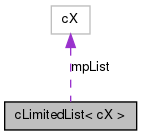
\includegraphics[width=178pt]{classc_limited_list__coll__graph}
\end{center}
\end{figure}
\subsection*{Public Member Functions}
\begin{DoxyCompactItemize}
\item 
void \hyperlink{classc_limited_list_ad909f4fc3256bfa9bc83b9baef8cac80}{ChangeSize} (uint32 liSize)
\item 
\hyperlink{classc_limited_list_a56cdd868a5924449791625ed2e462b03}{cLimitedList} ()
\item 
void \hyperlink{classc_limited_list_a29c4134a24a54d2d57498bb67447446e}{Init} (uint32 liSpaces)
\item 
\hyperlink{classc_limited_list_ae7c757c09f497da319f989e2042d488f}{cLimitedList} (uint32 liSpaces)
\item 
\hyperlink{classc_limited_list_ab7b63990b25112ae8cbf877b4fce7eed}{$\sim$cLimitedList} ()
\item 
cX \& \hyperlink{classc_limited_list_ae11b7c0a82de56c938eaf6d814838048}{operator\mbox{[}$\,$\mbox{]}} (uint32 liItem)
\item 
\hyperlink{classc_limited_list}{cLimitedList}$<$ cX $>$ \& \hyperlink{classc_limited_list_af6efd3116def79b9ca62cccc7ded030f}{operator=} (\hyperlink{classc_limited_list}{cLimitedList}$<$ cX $>$ \&lpOther)
\item 
uint32 \hyperlink{classc_limited_list_a0109c9831d7bf20d5ba259fc188be714}{Items} ()
\item 
void \hyperlink{classc_limited_list_a8a01caffbb1d69abf97481f12e59768d}{SetItems} (uint32 liItems)
\item 
void \hyperlink{classc_limited_list_a71e9c546a89a1be5cd656cc1284b4475}{Add} (cX $\ast$lpTemp)
\item 
void \hyperlink{classc_limited_list_a944c6ae2b1e13a144cc384766f9c12ae}{Remove} (uint32 liPos)
\item 
void \hyperlink{classc_limited_list_a378286ba482d356510d9a7a7b00395d9}{SwitchItems} (uint32 li1, uint32 li2)
\end{DoxyCompactItemize}
\subsection*{Public Attributes}
\begin{DoxyCompactItemize}
\item 
cX $\ast$ \hyperlink{classc_limited_list_aa3b0a10ecf4169b9bd7b41b0152e6a6a}{mpList}
\item 
uint32 \hyperlink{classc_limited_list_add31decc488d48f0037fe57a56c9aa4a}{miSpaces}
\item 
uint32 \hyperlink{classc_limited_list_a9509f6f3a5d9ad28608fbf288e43cf37}{miItems}
\end{DoxyCompactItemize}


\subsection{Detailed Description}
\subsubsection*{template$<$class cX$>$ class cLimitedList$<$ cX $>$}



Definition at line 5 of file WTLimitedList.h.



\subsection{Constructor \& Destructor Documentation}
\hypertarget{classc_limited_list_a56cdd868a5924449791625ed2e462b03}{
\index{cLimitedList@{cLimitedList}!cLimitedList@{cLimitedList}}
\index{cLimitedList@{cLimitedList}!cLimitedList@{cLimitedList}}
\subsubsection[{cLimitedList}]{\setlength{\rightskip}{0pt plus 5cm}template$<$class cX$>$ {\bf cLimitedList}$<$ cX $>$::{\bf cLimitedList} (
\begin{DoxyParamCaption}
{}
\end{DoxyParamCaption}
)\hspace{0.3cm}{\ttfamily  \mbox{[}inline\mbox{]}}}}
\label{classc_limited_list_a56cdd868a5924449791625ed2e462b03}


Definition at line 29 of file WTLimitedList.h.

\hypertarget{classc_limited_list_ae7c757c09f497da319f989e2042d488f}{
\index{cLimitedList@{cLimitedList}!cLimitedList@{cLimitedList}}
\index{cLimitedList@{cLimitedList}!cLimitedList@{cLimitedList}}
\subsubsection[{cLimitedList}]{\setlength{\rightskip}{0pt plus 5cm}template$<$class cX$>$ {\bf cLimitedList}$<$ cX $>$::{\bf cLimitedList} (
\begin{DoxyParamCaption}
\item[{uint32}]{liSpaces}
\end{DoxyParamCaption}
)\hspace{0.3cm}{\ttfamily  \mbox{[}inline\mbox{]}}}}
\label{classc_limited_list_ae7c757c09f497da319f989e2042d488f}


Definition at line 43 of file WTLimitedList.h.

\hypertarget{classc_limited_list_ab7b63990b25112ae8cbf877b4fce7eed}{
\index{cLimitedList@{cLimitedList}!$\sim$cLimitedList@{$\sim$cLimitedList}}
\index{$\sim$cLimitedList@{$\sim$cLimitedList}!cLimitedList@{cLimitedList}}
\subsubsection[{$\sim$cLimitedList}]{\setlength{\rightskip}{0pt plus 5cm}template$<$class cX$>$ {\bf cLimitedList}$<$ cX $>$::$\sim${\bf cLimitedList} (
\begin{DoxyParamCaption}
{}
\end{DoxyParamCaption}
)\hspace{0.3cm}{\ttfamily  \mbox{[}inline\mbox{]}}}}
\label{classc_limited_list_ab7b63990b25112ae8cbf877b4fce7eed}


Definition at line 48 of file WTLimitedList.h.



\subsection{Member Function Documentation}
\hypertarget{classc_limited_list_a71e9c546a89a1be5cd656cc1284b4475}{
\index{cLimitedList@{cLimitedList}!Add@{Add}}
\index{Add@{Add}!cLimitedList@{cLimitedList}}
\subsubsection[{Add}]{\setlength{\rightskip}{0pt plus 5cm}template$<$class cX$>$ void {\bf cLimitedList}$<$ cX $>$::Add (
\begin{DoxyParamCaption}
\item[{cX $\ast$}]{lpTemp}
\end{DoxyParamCaption}
)\hspace{0.3cm}{\ttfamily  \mbox{[}inline\mbox{]}}}}
\label{classc_limited_list_a71e9c546a89a1be5cd656cc1284b4475}


Definition at line 74 of file WTLimitedList.h.

\hypertarget{classc_limited_list_ad909f4fc3256bfa9bc83b9baef8cac80}{
\index{cLimitedList@{cLimitedList}!ChangeSize@{ChangeSize}}
\index{ChangeSize@{ChangeSize}!cLimitedList@{cLimitedList}}
\subsubsection[{ChangeSize}]{\setlength{\rightskip}{0pt plus 5cm}template$<$class cX$>$ void {\bf cLimitedList}$<$ cX $>$::ChangeSize (
\begin{DoxyParamCaption}
\item[{uint32}]{liSize}
\end{DoxyParamCaption}
)\hspace{0.3cm}{\ttfamily  \mbox{[}inline\mbox{]}}}}
\label{classc_limited_list_ad909f4fc3256bfa9bc83b9baef8cac80}


Definition at line 15 of file WTLimitedList.h.

\hypertarget{classc_limited_list_a29c4134a24a54d2d57498bb67447446e}{
\index{cLimitedList@{cLimitedList}!Init@{Init}}
\index{Init@{Init}!cLimitedList@{cLimitedList}}
\subsubsection[{Init}]{\setlength{\rightskip}{0pt plus 5cm}template$<$class cX$>$ void {\bf cLimitedList}$<$ cX $>$::Init (
\begin{DoxyParamCaption}
\item[{uint32}]{liSpaces}
\end{DoxyParamCaption}
)\hspace{0.3cm}{\ttfamily  \mbox{[}inline\mbox{]}}}}
\label{classc_limited_list_a29c4134a24a54d2d57498bb67447446e}


Definition at line 31 of file WTLimitedList.h.

\hypertarget{classc_limited_list_a0109c9831d7bf20d5ba259fc188be714}{
\index{cLimitedList@{cLimitedList}!Items@{Items}}
\index{Items@{Items}!cLimitedList@{cLimitedList}}
\subsubsection[{Items}]{\setlength{\rightskip}{0pt plus 5cm}template$<$class cX$>$ uint32 {\bf cLimitedList}$<$ cX $>$::Items (
\begin{DoxyParamCaption}
{}
\end{DoxyParamCaption}
)\hspace{0.3cm}{\ttfamily  \mbox{[}inline\mbox{]}}}}
\label{classc_limited_list_a0109c9831d7bf20d5ba259fc188be714}


Definition at line 71 of file WTLimitedList.h.

\hypertarget{classc_limited_list_af6efd3116def79b9ca62cccc7ded030f}{
\index{cLimitedList@{cLimitedList}!operator=@{operator=}}
\index{operator=@{operator=}!cLimitedList@{cLimitedList}}
\subsubsection[{operator=}]{\setlength{\rightskip}{0pt plus 5cm}template$<$class cX$>$ {\bf cLimitedList}$<$cX$>$\& {\bf cLimitedList}$<$ cX $>$::operator= (
\begin{DoxyParamCaption}
\item[{{\bf cLimitedList}$<$ cX $>$ \&}]{lpOther}
\end{DoxyParamCaption}
)\hspace{0.3cm}{\ttfamily  \mbox{[}inline\mbox{]}}}}
\label{classc_limited_list_af6efd3116def79b9ca62cccc7ded030f}


Definition at line 57 of file WTLimitedList.h.

\hypertarget{classc_limited_list_ae11b7c0a82de56c938eaf6d814838048}{
\index{cLimitedList@{cLimitedList}!operator\mbox{[}\mbox{]}@{operator[]}}
\index{operator\mbox{[}\mbox{]}@{operator[]}!cLimitedList@{cLimitedList}}
\subsubsection[{operator[]}]{\setlength{\rightskip}{0pt plus 5cm}template$<$class cX$>$ cX\& {\bf cLimitedList}$<$ cX $>$::operator\mbox{[}$\,$\mbox{]} (
\begin{DoxyParamCaption}
\item[{uint32}]{liItem}
\end{DoxyParamCaption}
)\hspace{0.3cm}{\ttfamily  \mbox{[}inline\mbox{]}}}}
\label{classc_limited_list_ae11b7c0a82de56c938eaf6d814838048}


Definition at line 55 of file WTLimitedList.h.

\hypertarget{classc_limited_list_a944c6ae2b1e13a144cc384766f9c12ae}{
\index{cLimitedList@{cLimitedList}!Remove@{Remove}}
\index{Remove@{Remove}!cLimitedList@{cLimitedList}}
\subsubsection[{Remove}]{\setlength{\rightskip}{0pt plus 5cm}template$<$class cX$>$ void {\bf cLimitedList}$<$ cX $>$::Remove (
\begin{DoxyParamCaption}
\item[{uint32}]{liPos}
\end{DoxyParamCaption}
)\hspace{0.3cm}{\ttfamily  \mbox{[}inline\mbox{]}}}}
\label{classc_limited_list_a944c6ae2b1e13a144cc384766f9c12ae}


Definition at line 76 of file WTLimitedList.h.

\hypertarget{classc_limited_list_a8a01caffbb1d69abf97481f12e59768d}{
\index{cLimitedList@{cLimitedList}!SetItems@{SetItems}}
\index{SetItems@{SetItems}!cLimitedList@{cLimitedList}}
\subsubsection[{SetItems}]{\setlength{\rightskip}{0pt plus 5cm}template$<$class cX$>$ void {\bf cLimitedList}$<$ cX $>$::SetItems (
\begin{DoxyParamCaption}
\item[{uint32}]{liItems}
\end{DoxyParamCaption}
)\hspace{0.3cm}{\ttfamily  \mbox{[}inline\mbox{]}}}}
\label{classc_limited_list_a8a01caffbb1d69abf97481f12e59768d}


Definition at line 72 of file WTLimitedList.h.

\hypertarget{classc_limited_list_a378286ba482d356510d9a7a7b00395d9}{
\index{cLimitedList@{cLimitedList}!SwitchItems@{SwitchItems}}
\index{SwitchItems@{SwitchItems}!cLimitedList@{cLimitedList}}
\subsubsection[{SwitchItems}]{\setlength{\rightskip}{0pt plus 5cm}template$<$class cX$>$ void {\bf cLimitedList}$<$ cX $>$::SwitchItems (
\begin{DoxyParamCaption}
\item[{uint32}]{li1, }
\item[{uint32}]{li2}
\end{DoxyParamCaption}
)\hspace{0.3cm}{\ttfamily  \mbox{[}inline\mbox{]}}}}
\label{classc_limited_list_a378286ba482d356510d9a7a7b00395d9}


Definition at line 86 of file WTLimitedList.h.



\subsection{Member Data Documentation}
\hypertarget{classc_limited_list_a9509f6f3a5d9ad28608fbf288e43cf37}{
\index{cLimitedList@{cLimitedList}!miItems@{miItems}}
\index{miItems@{miItems}!cLimitedList@{cLimitedList}}
\subsubsection[{miItems}]{\setlength{\rightskip}{0pt plus 5cm}template$<$class cX$>$ uint32 {\bf cLimitedList}$<$ cX $>$::{\bf miItems}}}
\label{classc_limited_list_a9509f6f3a5d9ad28608fbf288e43cf37}


Definition at line 13 of file WTLimitedList.h.

\hypertarget{classc_limited_list_add31decc488d48f0037fe57a56c9aa4a}{
\index{cLimitedList@{cLimitedList}!miSpaces@{miSpaces}}
\index{miSpaces@{miSpaces}!cLimitedList@{cLimitedList}}
\subsubsection[{miSpaces}]{\setlength{\rightskip}{0pt plus 5cm}template$<$class cX$>$ uint32 {\bf cLimitedList}$<$ cX $>$::{\bf miSpaces}}}
\label{classc_limited_list_add31decc488d48f0037fe57a56c9aa4a}


Definition at line 12 of file WTLimitedList.h.

\hypertarget{classc_limited_list_aa3b0a10ecf4169b9bd7b41b0152e6a6a}{
\index{cLimitedList@{cLimitedList}!mpList@{mpList}}
\index{mpList@{mpList}!cLimitedList@{cLimitedList}}
\subsubsection[{mpList}]{\setlength{\rightskip}{0pt plus 5cm}template$<$class cX$>$ cX$\ast$ {\bf cLimitedList}$<$ cX $>$::{\bf mpList}}}
\label{classc_limited_list_aa3b0a10ecf4169b9bd7b41b0152e6a6a}


Definition at line 11 of file WTLimitedList.h.


\hypertarget{classc_limited_pointer_list}{
\section{cLimitedPointerList$<$ cX $>$ Class Template Reference}
\label{classc_limited_pointer_list}\index{cLimitedPointerList@{cLimitedPointerList}}
}


This is similar to the \hyperlink{classc_limited_list}{cLimitedList} template class, but will uses pointers. The type cX is the base type. When a pointer is handed to the array, the list will store the pointer to the item and 'take ownership' of the object. This means that the item is NOT copied and when the list is deleted Items 'owned' to by the list will be deleted. This also makes array manipulation and size changing quicker. It will expand to accomodate new items added to the array.  


\subsection*{Public Member Functions}
\begin{DoxyCompactItemize}
\item 
\hypertarget{classc_limited_pointer_list_a07bb790fa0cce46a4724f87445278a2a}{
\hyperlink{classc_limited_pointer_list_a07bb790fa0cce46a4724f87445278a2a}{cLimitedPointerList} (uint32 liSpaces)}
\label{classc_limited_pointer_list_a07bb790fa0cce46a4724f87445278a2a}

\begin{DoxyCompactList}\small\item\em Constructor to create a new array of size liSpaces. \end{DoxyCompactList}\item 
\hypertarget{classc_limited_pointer_list_ad423e1b82ff902578d76e1e8ba33407f}{
\hyperlink{classc_limited_pointer_list_ad423e1b82ff902578d76e1e8ba33407f}{cLimitedPointerList} ()}
\label{classc_limited_pointer_list_ad423e1b82ff902578d76e1e8ba33407f}

\begin{DoxyCompactList}\small\item\em Constructor to create a 0 length array. \end{DoxyCompactList}\item 
\hypertarget{classc_limited_pointer_list_ab72b03a5d82ee318bf21d3102bdfecda}{
void \hyperlink{classc_limited_pointer_list_ab72b03a5d82ee318bf21d3102bdfecda}{Init} (uint32 liSpaces)}
\label{classc_limited_pointer_list_ab72b03a5d82ee318bf21d3102bdfecda}

\begin{DoxyCompactList}\small\item\em This will initialise the array to size liSpaces. \end{DoxyCompactList}\item 
\hypertarget{classc_limited_pointer_list_a7d77c2291a85cb39f06776e8d8555030}{
void \hyperlink{classc_limited_pointer_list_a7d77c2291a85cb39f06776e8d8555030}{ChangeSize} (uint32 liSize)}
\label{classc_limited_pointer_list_a7d77c2291a85cb39f06776e8d8555030}

\begin{DoxyCompactList}\small\item\em This will change the array size to liSize. Pointers will be copied across. If the new array is too short to store all the data. The excess objects will be deleted. \end{DoxyCompactList}\item 
\hypertarget{classc_limited_pointer_list_a5cd2eaf04fa51a23e35bb78ba875501f}{
void \hyperlink{classc_limited_pointer_list_a5cd2eaf04fa51a23e35bb78ba875501f}{DeleteAll} ()}
\label{classc_limited_pointer_list_a5cd2eaf04fa51a23e35bb78ba875501f}

\begin{DoxyCompactList}\small\item\em This will delete all items in the list. Clear the list to size 0. It will not delete this list object. \end{DoxyCompactList}\item 
\hypertarget{classc_limited_pointer_list_a4aef178a850d901cefc169cd0f8b1e71}{
\hyperlink{classc_limited_pointer_list_a4aef178a850d901cefc169cd0f8b1e71}{$\sim$cLimitedPointerList} ()}
\label{classc_limited_pointer_list_a4aef178a850d901cefc169cd0f8b1e71}

\begin{DoxyCompactList}\small\item\em Deconstructor for this list object. This will calll \hyperlink{classc_limited_pointer_list_a5cd2eaf04fa51a23e35bb78ba875501f}{DeleteAll()} \end{DoxyCompactList}\item 
\hypertarget{classc_limited_pointer_list_a118f2d5687c97cf122b163dbbdedb56d}{
cX $\ast$ \hyperlink{classc_limited_pointer_list_a118f2d5687c97cf122b163dbbdedb56d}{operator\mbox{[}$\,$\mbox{]}} (uint32 liItem)}
\label{classc_limited_pointer_list_a118f2d5687c97cf122b163dbbdedb56d}

\begin{DoxyCompactList}\small\item\em \mbox{[}\mbox{]} operatr to allow this to be used like a pointer array. \end{DoxyCompactList}\item 
\hypertarget{classc_limited_pointer_list_a00af27280f0a9d3f89fa8b9da36b7554}{
cX $\ast$ \hyperlink{classc_limited_pointer_list_a00af27280f0a9d3f89fa8b9da36b7554}{Item} (uint32 liItem)}
\label{classc_limited_pointer_list_a00af27280f0a9d3f89fa8b9da36b7554}

\begin{DoxyCompactList}\small\item\em Will return the pointer at position liItem in the list. \end{DoxyCompactList}\item 
\hypertarget{classc_limited_pointer_list_a0ba95ea83cbfee5957645c711ccab08c}{
void \hyperlink{classc_limited_pointer_list_a0ba95ea83cbfee5957645c711ccab08c}{Add} (cX $\ast$lpValue)}
\label{classc_limited_pointer_list_a0ba95ea83cbfee5957645c711ccab08c}

\begin{DoxyCompactList}\small\item\em Will Add the pointer lpValue to the list. Once added the Array will control deleting the object pointed to by lpValue. It will also expand the array to acomodate the item as required. \end{DoxyCompactList}\item 
\hypertarget{classc_limited_pointer_list_a61fdd759615a826b5f385ad0b9ddfb0d}{
void \hyperlink{classc_limited_pointer_list_a61fdd759615a826b5f385ad0b9ddfb0d}{Remove} (uint32 liPos)}
\label{classc_limited_pointer_list_a61fdd759615a826b5f385ad0b9ddfb0d}

\begin{DoxyCompactList}\small\item\em This will remove the item liPos from the List. It will delete the item and shuffle all the other items in teh list to the front of the list. \end{DoxyCompactList}\item 
\hypertarget{classc_limited_pointer_list_ad2981a22dcb5e79790b8644125cc7322}{
void \hyperlink{classc_limited_pointer_list_ad2981a22dcb5e79790b8644125cc7322}{SwitchItems} (uint32 li1, uint32 li2)}
\label{classc_limited_pointer_list_ad2981a22dcb5e79790b8644125cc7322}

\begin{DoxyCompactList}\small\item\em This will switch the positions of the items at positions li1 and li2 in the list. \end{DoxyCompactList}\end{DoxyCompactItemize}


\subsection{Detailed Description}
\subsubsection*{template$<$class cX$>$class cLimitedPointerList$<$ cX $>$}

This is similar to the \hyperlink{classc_limited_list}{cLimitedList} template class, but will uses pointers. The type cX is the base type. When a pointer is handed to the array, the list will store the pointer to the item and 'take ownership' of the object. This means that the item is NOT copied and when the list is deleted Items 'owned' to by the list will be deleted. This also makes array manipulation and size changing quicker. It will expand to accomodate new items added to the array. 
\hypertarget{classc_line}{
\section{cLine Class Reference}
\label{classc_line}\index{cLine@{cLine}}
}


A standard renderable Line object.  




Collaboration diagram for cLine:\nopagebreak
\begin{figure}[H]
\begin{center}
\leavevmode
\includegraphics[height=600pt]{classc_line__coll__graph}
\end{center}
\end{figure}
\subsection*{Public Member Functions}
\begin{DoxyCompactItemize}
\item 
\hypertarget{classc_line_afc96602bef17f3d03af9685532af395d}{
\hyperlink{classc_line_afc96602bef17f3d03af9685532af395d}{cLine} ()}
\label{classc_line_afc96602bef17f3d03af9685532af395d}

\begin{DoxyCompactList}\small\item\em \hyperlink{classc_line}{cLine} constructor \end{DoxyCompactList}\item 
\hypertarget{classc_line_aa9c1d8af366fbcd7e5f71e82906a1b2c}{
\hyperlink{classc_line_aa9c1d8af366fbcd7e5f71e82906a1b2c}{cLine} (vRenderNode $\ast$lpRenderer)}
\label{classc_line_aa9c1d8af366fbcd7e5f71e82906a1b2c}

\begin{DoxyCompactList}\small\item\em \hyperlink{classc_line}{cLine} constructor. Will be owned by lpRenderer. \end{DoxyCompactList}\item 
\hypertarget{classc_line_a8a84cc1fe6a5a875faece391612347fc}{
\hyperlink{classc_line_a8a84cc1fe6a5a875faece391612347fc}{cLine} (\hyperlink{classc_camera}{cCamera} $\ast$lpCamera)}
\label{classc_line_a8a84cc1fe6a5a875faece391612347fc}

\begin{DoxyCompactList}\small\item\em \hyperlink{classc_line}{cLine} constructor. Will be owned by the \hyperlink{classc_render_node}{cRenderNode} of the \hyperlink{classc_camera}{cCamera} lpCamera. \end{DoxyCompactList}\item 
\hypertarget{classc_line_a32342ae3b470044b21f38f3fe3e0c232}{
float $\ast$ \hyperlink{classc_line_a32342ae3b470044b21f38f3fe3e0c232}{Position} ()}
\label{classc_line_a32342ae3b470044b21f38f3fe3e0c232}

\begin{DoxyCompactList}\small\item\em Will return a pointer to the position of this line object (XYZ). \end{DoxyCompactList}\item 
\hypertarget{classc_line_acfefe5128253475e8291d110f004095b}{
void \hyperlink{classc_line_acfefe5128253475e8291d110f004095b}{Position} (float $\ast$lfPos)}
\label{classc_line_acfefe5128253475e8291d110f004095b}

\begin{DoxyCompactList}\small\item\em Will set the position of this object to the float array pointed to by lfPos. Expects 3 floats (XYZ). \end{DoxyCompactList}\item 
\hypertarget{classc_line_aedeac0c1874b8212e8cc878b920513d9}{
void \hyperlink{classc_line_aedeac0c1874b8212e8cc878b920513d9}{Position} (float lfX, float lfY, float lfZ=0.0f)}
\label{classc_line_aedeac0c1874b8212e8cc878b920513d9}

\begin{DoxyCompactList}\small\item\em Will set the position of this object to the values specified (XYZ). \end{DoxyCompactList}\item 
\hypertarget{classc_line_a4b37bd0ff6ea3834a2c49d5efbd222c9}{
float $\ast$ \hyperlink{classc_line_a4b37bd0ff6ea3834a2c49d5efbd222c9}{Vector} ()}
\label{classc_line_a4b37bd0ff6ea3834a2c49d5efbd222c9}

\begin{DoxyCompactList}\small\item\em Will return a pointer to the vector of this line object (XYZ). \end{DoxyCompactList}\item 
\hypertarget{classc_line_ad558bfa28a78a6594446ae0c5e11c262}{
void \hyperlink{classc_line_ad558bfa28a78a6594446ae0c5e11c262}{Vector} (float $\ast$lfPos)}
\label{classc_line_ad558bfa28a78a6594446ae0c5e11c262}

\begin{DoxyCompactList}\small\item\em Will set the vector of this object to the float array pointed to by lfPos. Expects 3 floats (XYZ). \end{DoxyCompactList}\item 
\hypertarget{classc_line_abfbbb77ed5b1c9208baf6d38b907b7b5}{
void \hyperlink{classc_line_abfbbb77ed5b1c9208baf6d38b907b7b5}{Vector} (float lfX, float lfY, float lfZ=0.0f)}
\label{classc_line_abfbbb77ed5b1c9208baf6d38b907b7b5}

\begin{DoxyCompactList}\small\item\em Will set the vector of this object to the values specified (XYZ). \end{DoxyCompactList}\item 
\hypertarget{classc_line_a4b02fb7febded866cc8fda351d623811}{
void \hyperlink{classc_line_a4b02fb7febded866cc8fda351d623811}{Width} (float lfWidth)}
\label{classc_line_a4b02fb7febded866cc8fda351d623811}

\begin{DoxyCompactList}\small\item\em Will set the width for the line. \end{DoxyCompactList}\item 
\hypertarget{classc_line_a26247a346a469646b250fa0116e1ec34}{
float \hyperlink{classc_line_a26247a346a469646b250fa0116e1ec34}{Width} ()}
\label{classc_line_a26247a346a469646b250fa0116e1ec34}

\begin{DoxyCompactList}\small\item\em Will return the lines width. \end{DoxyCompactList}\end{DoxyCompactItemize}


\subsection{Detailed Description}
A standard renderable Line object. 
\hypertarget{classc_linked_list}{
\section{cLinkedList$<$ T $>$ Class Template Reference}
\label{classc_linked_list}\index{cLinkedList@{cLinkedList}}
}


This is the control for a linked list. It controls a linked list of cLinkedNodes which each point to their item in the list. Each \hyperlink{classc_linked_node}{cLinkedNode} poitns to the \hyperlink{classc_linked_node}{cLinkedNode} s either side of themselves and the data they own. \hyperlink{classc_linked_list}{cLinkedList} is templated and so can be a linked list of any type.  


\subsection*{Public Member Functions}
\begin{DoxyCompactItemize}
\item 
void \hyperlink{classc_linked_list_a57cda13916eac63747ff70071907d7ca}{StitchOut} (\hyperlink{classc_linked_node}{cLinkedNode}$<$ T $>$ $\ast$lpNode)
\item 
void \hyperlink{classc_linked_list_adf5505edbd4933ccde08183c539e6655}{StitchIn} (\hyperlink{classc_linked_node}{cLinkedNode}$<$ T $>$ $\ast$lpNode)
\item 
void \hyperlink{classc_linked_list_acdd0ec24de3bc0a706e1ec8b4a2cb2ae}{StitchIn} (\hyperlink{classc_linked_node}{cLinkedNode}$<$ T $>$ $\ast$lpNode, \hyperlink{classc_linked_node}{cLinkedNode}$<$ T $>$ $\ast$lpPos)
\item 
\hyperlink{classc_linked_list_adbdde7829ddb9dc0518126d8e0164e10}{cLinkedList} (T $\ast$lpData)
\begin{DoxyCompactList}\small\item\em This holds a pointer of the relevant type for the list and will create the list by making the item lpData the first item in the list. \item\end{DoxyCompactList}\item 
\hyperlink{classc_linked_list_a2aacceb9a6498158af9598cb424977e3}{cLinkedList} ()
\item 
\hyperlink{classc_linked_list_a80aef75883bffae5da5ee7d8b9258502}{$\sim$cLinkedList} ()
\begin{DoxyCompactList}\small\item\em This will delete the list and delete every item in the list. \item\end{DoxyCompactList}\item 
\hyperlink{classc_linked_node}{cLinkedNode}$<$ T $>$ $\ast$ \hyperlink{classc_linked_list_a91593c408e5c5fc719624531f996c29c}{Start} ()
\item 
\hyperlink{classc_linked_node}{cLinkedNode}$<$ T $>$ $\ast$ \hyperlink{classc_linked_list_a95267afd7cde82576255fbde914a7e0d}{End} ()
\item 
\hyperlink{classc_linked_node}{cLinkedNode}$<$ T $>$ $\ast$ \hyperlink{classc_linked_list_a6014141bbd16b32e22b4b7deb873f1ae}{Find} (T $\ast$lpData)
\begin{DoxyCompactList}\small\item\em This is the number of items in the list. \item\end{DoxyCompactList}\item 
\hyperlink{classc_linked_node}{cLinkedNode}$<$ T $>$ $\ast$ \hyperlink{classc_linked_list_ae9bedf047bccf0f63b10b662c809032c}{Insert} (T $\ast$lpData)
\begin{DoxyCompactList}\small\item\em This will create a \hyperlink{classc_linked_node}{cLinkedNode} give it lpData and add that node to the end of the list. \item\end{DoxyCompactList}\item 
void \hyperlink{classc_linked_list_ab4694aa48324f52b8b1c25eb43dc996c}{Delete} (\hyperlink{classc_linked_node}{cLinkedNode}$<$ T $>$ $\ast$lpOld)
\begin{DoxyCompactList}\small\item\em This will delete the \hyperlink{classc_linked_node}{cLinkedNode} pointed to by lpOld and remove it from the list including mpData. \item\end{DoxyCompactList}\item 
void \hyperlink{classc_linked_list_a1806f7d9fcba9d78f54b2787919d5407}{Initialise} ()
\item 
void \hyperlink{classc_linked_list_a4f6cff87d2c90874949757987f6b9748}{Move} (\hyperlink{classc_linked_node}{cLinkedNode}$<$ T $>$ $\ast$lpFrom, \hyperlink{classc_linked_node}{cLinkedNode}$<$ T $>$ $\ast$lpPosition)
\begin{DoxyCompactList}\small\item\em This will Move the node lpFrom to be before lpPosition. \item\end{DoxyCompactList}\item 
void \hyperlink{classc_linked_list_ad62406784a55a3477383c51a59ec7603}{Move} (\hyperlink{classc_linked_node}{cLinkedNode}$<$ T $>$ $\ast$lpFrom, \hyperlink{classc_linked_list}{cLinkedList}$<$ T $>$ $\ast$lpPosition)
\item 
void \hyperlink{classc_linked_list_a48b99bef680a675623c84684c17691a6}{ClearAll} ()
\item 
void \hyperlink{classc_linked_list_a6116806e9435ffde67f1c26f1138e431}{DeleteAll} ()
\item 
void \hyperlink{classc_linked_list_a476170cb815fe62c516fc3fb439d9c19}{Display} ()
\item 
void \hyperlink{classc_linked_list_a676cd3bd124df98773c296ed6f67ba16}{Remove} (\hyperlink{classc_linked_node}{cLinkedNode}$<$ T $>$ $\ast$lpNode)
\begin{DoxyCompactList}\small\item\em This will delete the \hyperlink{classc_linked_node}{cLinkedNode} pointed to by lpOld and remove it from the list, but not delete mpData. \item\end{DoxyCompactList}\end{DoxyCompactItemize}
\subsection*{Static Public Attributes}
\begin{DoxyCompactItemize}
\item 
static \hyperlink{classc_linked_node}{cLinkedNode}$<$ T $>$ $\ast$ \hyperlink{classc_linked_list_abc440dbcbff9bcfb6e538a0e008c27c1}{mpTemp} = 0
\begin{DoxyCompactList}\small\item\em This is a pointer that can be used as a cursor by this linked list. \item\end{DoxyCompactList}\end{DoxyCompactItemize}


\subsection{Detailed Description}
\subsubsection*{template$<$class T$>$ class cLinkedList$<$ T $>$}

This is the control for a linked list. It controls a linked list of cLinkedNodes which each point to their item in the list. Each \hyperlink{classc_linked_node}{cLinkedNode} poitns to the \hyperlink{classc_linked_node}{cLinkedNode} s either side of themselves and the data they own. \hyperlink{classc_linked_list}{cLinkedList} is templated and so can be a linked list of any type. 

Definition at line 50 of file WTLLTemplate.h.



\subsection{Constructor \& Destructor Documentation}
\hypertarget{classc_linked_list_adbdde7829ddb9dc0518126d8e0164e10}{
\index{cLinkedList@{cLinkedList}!cLinkedList@{cLinkedList}}
\index{cLinkedList@{cLinkedList}!cLinkedList@{cLinkedList}}
\subsubsection[{cLinkedList}]{\setlength{\rightskip}{0pt plus 5cm}template$<$class T$>$ {\bf cLinkedList}$<$ T $>$::{\bf cLinkedList} (
\begin{DoxyParamCaption}
\item[{T $\ast$}]{lpData}
\end{DoxyParamCaption}
)}}
\label{classc_linked_list_adbdde7829ddb9dc0518126d8e0164e10}


This holds a pointer of the relevant type for the list and will create the list by making the item lpData the first item in the list. 



Definition at line 276 of file WTLLTemplate.h.

\hypertarget{classc_linked_list_a2aacceb9a6498158af9598cb424977e3}{
\index{cLinkedList@{cLinkedList}!cLinkedList@{cLinkedList}}
\index{cLinkedList@{cLinkedList}!cLinkedList@{cLinkedList}}
\subsubsection[{cLinkedList}]{\setlength{\rightskip}{0pt plus 5cm}template$<$class T$>$ {\bf cLinkedList}$<$ T $>$::{\bf cLinkedList} (
\begin{DoxyParamCaption}
{}
\end{DoxyParamCaption}
)}}
\label{classc_linked_list_a2aacceb9a6498158af9598cb424977e3}


Definition at line 183 of file WTLLTemplate.h.

\hypertarget{classc_linked_list_a80aef75883bffae5da5ee7d8b9258502}{
\index{cLinkedList@{cLinkedList}!$\sim$cLinkedList@{$\sim$cLinkedList}}
\index{$\sim$cLinkedList@{$\sim$cLinkedList}!cLinkedList@{cLinkedList}}
\subsubsection[{$\sim$cLinkedList}]{\setlength{\rightskip}{0pt plus 5cm}template$<$class T$>$ {\bf cLinkedList}$<$ T $>$::$\sim${\bf cLinkedList} (
\begin{DoxyParamCaption}
{}
\end{DoxyParamCaption}
)\hspace{0.3cm}{\ttfamily  \mbox{[}inline\mbox{]}}}}
\label{classc_linked_list_a80aef75883bffae5da5ee7d8b9258502}


This will delete the list and delete every item in the list. 



Definition at line 68 of file WTLLTemplate.h.



\subsection{Member Function Documentation}
\hypertarget{classc_linked_list_a48b99bef680a675623c84684c17691a6}{
\index{cLinkedList@{cLinkedList}!ClearAll@{ClearAll}}
\index{ClearAll@{ClearAll}!cLinkedList@{cLinkedList}}
\subsubsection[{ClearAll}]{\setlength{\rightskip}{0pt plus 5cm}template$<$class T $>$ void {\bf cLinkedList}$<$ T $>$::ClearAll (
\begin{DoxyParamCaption}
{}
\end{DoxyParamCaption}
)}}
\label{classc_linked_list_a48b99bef680a675623c84684c17691a6}


Definition at line 189 of file WTLLTemplate.h.

\hypertarget{classc_linked_list_ab4694aa48324f52b8b1c25eb43dc996c}{
\index{cLinkedList@{cLinkedList}!Delete@{Delete}}
\index{Delete@{Delete}!cLinkedList@{cLinkedList}}
\subsubsection[{Delete}]{\setlength{\rightskip}{0pt plus 5cm}template$<$class T$>$ void {\bf cLinkedList}$<$ T $>$::Delete (
\begin{DoxyParamCaption}
\item[{{\bf cLinkedNode}$<$ T $>$ $\ast$}]{lpOld}
\end{DoxyParamCaption}
)}}
\label{classc_linked_list_ab4694aa48324f52b8b1c25eb43dc996c}


This will delete the \hyperlink{classc_linked_node}{cLinkedNode} pointed to by lpOld and remove it from the list including mpData. 



Definition at line 226 of file WTLLTemplate.h.

\hypertarget{classc_linked_list_a6116806e9435ffde67f1c26f1138e431}{
\index{cLinkedList@{cLinkedList}!DeleteAll@{DeleteAll}}
\index{DeleteAll@{DeleteAll}!cLinkedList@{cLinkedList}}
\subsubsection[{DeleteAll}]{\setlength{\rightskip}{0pt plus 5cm}template$<$class T $>$ void {\bf cLinkedList}$<$ T $>$::DeleteAll (
\begin{DoxyParamCaption}
{}
\end{DoxyParamCaption}
)}}
\label{classc_linked_list_a6116806e9435ffde67f1c26f1138e431}


Definition at line 116 of file WTLLTemplate.h.

\hypertarget{classc_linked_list_a476170cb815fe62c516fc3fb439d9c19}{
\index{cLinkedList@{cLinkedList}!Display@{Display}}
\index{Display@{Display}!cLinkedList@{cLinkedList}}
\subsubsection[{Display}]{\setlength{\rightskip}{0pt plus 5cm}template$<$class T $>$ void {\bf cLinkedList}$<$ T $>$::Display (
\begin{DoxyParamCaption}
{}
\end{DoxyParamCaption}
)}}
\label{classc_linked_list_a476170cb815fe62c516fc3fb439d9c19}


Definition at line 300 of file WTLLTemplate.h.

\hypertarget{classc_linked_list_a95267afd7cde82576255fbde914a7e0d}{
\index{cLinkedList@{cLinkedList}!End@{End}}
\index{End@{End}!cLinkedList@{cLinkedList}}
\subsubsection[{End}]{\setlength{\rightskip}{0pt plus 5cm}template$<$class T$>$ {\bf cLinkedNode}$<$T$>$$\ast$ {\bf cLinkedList}$<$ T $>$::End (
\begin{DoxyParamCaption}
{}
\end{DoxyParamCaption}
)\hspace{0.3cm}{\ttfamily  \mbox{[}inline\mbox{]}}}}
\label{classc_linked_list_a95267afd7cde82576255fbde914a7e0d}


Definition at line 75 of file WTLLTemplate.h.

\hypertarget{classc_linked_list_a6014141bbd16b32e22b4b7deb873f1ae}{
\index{cLinkedList@{cLinkedList}!Find@{Find}}
\index{Find@{Find}!cLinkedList@{cLinkedList}}
\subsubsection[{Find}]{\setlength{\rightskip}{0pt plus 5cm}template$<$class T$>$ {\bf cLinkedNode}$<$ T $>$ $\ast$ {\bf cLinkedList}$<$ T $>$::Find (
\begin{DoxyParamCaption}
\item[{T $\ast$}]{lpData}
\end{DoxyParamCaption}
)}}
\label{classc_linked_list_a6014141bbd16b32e22b4b7deb873f1ae}


This is the number of items in the list. 

This will return the \hyperlink{classc_linked_node}{cLinkedNode} which owns the item lpData in this list. 

Definition at line 219 of file WTLLTemplate.h.

\hypertarget{classc_linked_list_a1806f7d9fcba9d78f54b2787919d5407}{
\index{cLinkedList@{cLinkedList}!Initialise@{Initialise}}
\index{Initialise@{Initialise}!cLinkedList@{cLinkedList}}
\subsubsection[{Initialise}]{\setlength{\rightskip}{0pt plus 5cm}template$<$class T $>$ void {\bf cLinkedList}$<$ T $>$::Initialise (
\begin{DoxyParamCaption}
{}
\end{DoxyParamCaption}
)}}
\label{classc_linked_list_a1806f7d9fcba9d78f54b2787919d5407}


Definition at line 107 of file WTLLTemplate.h.

\hypertarget{classc_linked_list_ae9bedf047bccf0f63b10b662c809032c}{
\index{cLinkedList@{cLinkedList}!Insert@{Insert}}
\index{Insert@{Insert}!cLinkedList@{cLinkedList}}
\subsubsection[{Insert}]{\setlength{\rightskip}{0pt plus 5cm}template$<$class T$>$ {\bf cLinkedNode}$<$ T $>$ $\ast$ {\bf cLinkedList}$<$ T $>$::Insert (
\begin{DoxyParamCaption}
\item[{T $\ast$}]{lpData}
\end{DoxyParamCaption}
)}}
\label{classc_linked_list_ae9bedf047bccf0f63b10b662c809032c}


This will create a \hyperlink{classc_linked_node}{cLinkedNode} give it lpData and add that node to the end of the list. 



Definition at line 289 of file WTLLTemplate.h.

\hypertarget{classc_linked_list_a4f6cff87d2c90874949757987f6b9748}{
\index{cLinkedList@{cLinkedList}!Move@{Move}}
\index{Move@{Move}!cLinkedList@{cLinkedList}}
\subsubsection[{Move}]{\setlength{\rightskip}{0pt plus 5cm}template$<$class T$>$ void {\bf cLinkedList}$<$ T $>$::Move (
\begin{DoxyParamCaption}
\item[{{\bf cLinkedNode}$<$ T $>$ $\ast$}]{lpFrom, }
\item[{{\bf cLinkedNode}$<$ T $>$ $\ast$}]{lpPosition}
\end{DoxyParamCaption}
)}}
\label{classc_linked_list_a4f6cff87d2c90874949757987f6b9748}


This will Move the node lpFrom to be before lpPosition. 

\hypertarget{classc_linked_list_ad62406784a55a3477383c51a59ec7603}{
\index{cLinkedList@{cLinkedList}!Move@{Move}}
\index{Move@{Move}!cLinkedList@{cLinkedList}}
\subsubsection[{Move}]{\setlength{\rightskip}{0pt plus 5cm}template$<$class T$>$ void {\bf cLinkedList}$<$ T $>$::Move (
\begin{DoxyParamCaption}
\item[{{\bf cLinkedNode}$<$ T $>$ $\ast$}]{lpFrom, }
\item[{{\bf cLinkedList}$<$ T $>$ $\ast$}]{lpPosition}
\end{DoxyParamCaption}
)}}
\label{classc_linked_list_ad62406784a55a3477383c51a59ec7603}


Definition at line 208 of file WTLLTemplate.h.

\hypertarget{classc_linked_list_a676cd3bd124df98773c296ed6f67ba16}{
\index{cLinkedList@{cLinkedList}!Remove@{Remove}}
\index{Remove@{Remove}!cLinkedList@{cLinkedList}}
\subsubsection[{Remove}]{\setlength{\rightskip}{0pt plus 5cm}template$<$class T$>$ void {\bf cLinkedList}$<$ T $>$::Remove (
\begin{DoxyParamCaption}
\item[{{\bf cLinkedNode}$<$ T $>$ $\ast$}]{lpNode}
\end{DoxyParamCaption}
)}}
\label{classc_linked_list_a676cd3bd124df98773c296ed6f67ba16}


This will delete the \hyperlink{classc_linked_node}{cLinkedNode} pointed to by lpOld and remove it from the list, but not delete mpData. 



Definition at line 155 of file WTLLTemplate.h.

\hypertarget{classc_linked_list_a91593c408e5c5fc719624531f996c29c}{
\index{cLinkedList@{cLinkedList}!Start@{Start}}
\index{Start@{Start}!cLinkedList@{cLinkedList}}
\subsubsection[{Start}]{\setlength{\rightskip}{0pt plus 5cm}template$<$class T$>$ {\bf cLinkedNode}$<$T$>$$\ast$ {\bf cLinkedList}$<$ T $>$::Start (
\begin{DoxyParamCaption}
{}
\end{DoxyParamCaption}
)\hspace{0.3cm}{\ttfamily  \mbox{[}inline\mbox{]}}}}
\label{classc_linked_list_a91593c408e5c5fc719624531f996c29c}


Definition at line 73 of file WTLLTemplate.h.

\hypertarget{classc_linked_list_adf5505edbd4933ccde08183c539e6655}{
\index{cLinkedList@{cLinkedList}!StitchIn@{StitchIn}}
\index{StitchIn@{StitchIn}!cLinkedList@{cLinkedList}}
\subsubsection[{StitchIn}]{\setlength{\rightskip}{0pt plus 5cm}template$<$class T$>$ void {\bf cLinkedList}$<$ T $>$::StitchIn (
\begin{DoxyParamCaption}
\item[{{\bf cLinkedNode}$<$ T $>$ $\ast$}]{lpNode}
\end{DoxyParamCaption}
)}}
\label{classc_linked_list_adf5505edbd4933ccde08183c539e6655}


Definition at line 235 of file WTLLTemplate.h.

\hypertarget{classc_linked_list_acdd0ec24de3bc0a706e1ec8b4a2cb2ae}{
\index{cLinkedList@{cLinkedList}!StitchIn@{StitchIn}}
\index{StitchIn@{StitchIn}!cLinkedList@{cLinkedList}}
\subsubsection[{StitchIn}]{\setlength{\rightskip}{0pt plus 5cm}template$<$class T$>$ void {\bf cLinkedList}$<$ T $>$::StitchIn (
\begin{DoxyParamCaption}
\item[{{\bf cLinkedNode}$<$ T $>$ $\ast$}]{lpNode, }
\item[{{\bf cLinkedNode}$<$ T $>$ $\ast$}]{lpPos}
\end{DoxyParamCaption}
)}}
\label{classc_linked_list_acdd0ec24de3bc0a706e1ec8b4a2cb2ae}


Definition at line 255 of file WTLLTemplate.h.

\hypertarget{classc_linked_list_a57cda13916eac63747ff70071907d7ca}{
\index{cLinkedList@{cLinkedList}!StitchOut@{StitchOut}}
\index{StitchOut@{StitchOut}!cLinkedList@{cLinkedList}}
\subsubsection[{StitchOut}]{\setlength{\rightskip}{0pt plus 5cm}template$<$class T$>$ void {\bf cLinkedList}$<$ T $>$::StitchOut (
\begin{DoxyParamCaption}
\item[{{\bf cLinkedNode}$<$ T $>$ $\ast$}]{lpNode}
\end{DoxyParamCaption}
)}}
\label{classc_linked_list_a57cda13916eac63747ff70071907d7ca}


Definition at line 163 of file WTLLTemplate.h.



\subsection{Member Data Documentation}
\hypertarget{classc_linked_list_abc440dbcbff9bcfb6e538a0e008c27c1}{
\index{cLinkedList@{cLinkedList}!mpTemp@{mpTemp}}
\index{mpTemp@{mpTemp}!cLinkedList@{cLinkedList}}
\subsubsection[{mpTemp}]{\setlength{\rightskip}{0pt plus 5cm}template$<$class T$>$ {\bf cLinkedNode}$<$ T $>$ $\ast$ {\bf cLinkedList}$<$ T $>$::{\bf mpTemp} = 0\hspace{0.3cm}{\ttfamily  \mbox{[}static\mbox{]}}}}
\label{classc_linked_list_abc440dbcbff9bcfb6e538a0e008c27c1}


This is a pointer that can be used as a cursor by this linked list. 



Definition at line 75 of file WTLLTemplate.h.


\hypertarget{classc_linked_node}{
\section{cLinkedNode$<$ T $>$ Class Template Reference}
\label{classc_linked_node}\index{cLinkedNode@{cLinkedNode}}
}


This is a node class to allow templating of the \hyperlink{classc_linked_list}{cLinkedList} class. This node will store pointers to the nodes either side of this node in the linked list and a pointer to the object his node owns.  




Collaboration diagram for cLinkedNode$<$ T $>$:\nopagebreak
\begin{figure}[H]
\begin{center}
\leavevmode
\includegraphics[width=231pt]{classc_linked_node__coll__graph}
\end{center}
\end{figure}
\subsection*{Public Member Functions}
\begin{DoxyCompactItemize}
\item 
\hypertarget{classc_linked_node_adb8af44378d6d47b439ec7950f579bb3}{
\hyperlink{classc_linked_node_adb8af44378d6d47b439ec7950f579bb3}{$\sim$cLinkedNode} ()}
\label{classc_linked_node_adb8af44378d6d47b439ec7950f579bb3}

\begin{DoxyCompactList}\small\item\em This will delete the data owned by this node as it is deconstructed. \end{DoxyCompactList}\item 
\hypertarget{classc_linked_node_ac375aeade4f13f07a601732e80b49e8b}{
\hyperlink{classc_linked_node}{cLinkedNode}$<$ T $>$ $\ast$ \hyperlink{classc_linked_node_ac375aeade4f13f07a601732e80b49e8b}{Next} ()}
\label{classc_linked_node_ac375aeade4f13f07a601732e80b49e8b}

\begin{DoxyCompactList}\small\item\em This will return a pointer to the next node in the linked list. see \hyperlink{classc_linked_list}{cLinkedList}. \end{DoxyCompactList}\item 
\hypertarget{classc_linked_node_a6481dec71a6adffa72fd9621f366253a}{
\hyperlink{classc_linked_node}{cLinkedNode}$<$ T $>$ $\ast$ \hyperlink{classc_linked_node_a6481dec71a6adffa72fd9621f366253a}{Previous} ()}
\label{classc_linked_node_a6481dec71a6adffa72fd9621f366253a}

\begin{DoxyCompactList}\small\item\em This will return a pointer to the previous node in the linked list. see \hyperlink{classc_linked_list}{cLinkedList}. \end{DoxyCompactList}\end{DoxyCompactItemize}
\subsection*{Friends}
\begin{DoxyCompactItemize}
\item 
\hypertarget{classc_linked_node_a5b538a518f67ed3377a26348f2b536da}{
class \hyperlink{classc_linked_node_a5b538a518f67ed3377a26348f2b536da}{cLinkedList$<$ T $>$}}
\label{classc_linked_node_a5b538a518f67ed3377a26348f2b536da}

\end{DoxyCompactItemize}


\subsection{Detailed Description}
\subsubsection*{template$<$class T$>$class cLinkedNode$<$ T $>$}

This is a node class to allow templating of the \hyperlink{classc_linked_list}{cLinkedList} class. This node will store pointers to the nodes either side of this node in the linked list and a pointer to the object his node owns. 
\hypertarget{classc_main_thread}{
\section{cMainThread$<$ cX, cS $>$ Class Template Reference}
\label{classc_main_thread}\index{cMainThread@{cMainThread}}
}
\subsection*{Public Member Functions}
\begin{DoxyCompactItemize}
\item 
\hyperlink{classc_main_thread_a6eb20e854fb31291be7cd3ca35a2c68c}{$\sim$cMainThread} ()
\item 
\hyperlink{classc_main_thread_a6eb20e854fb31291be7cd3ca35a2c68c}{$\sim$cMainThread} ()
\end{DoxyCompactItemize}
\subsection*{Static Public Member Functions}
\begin{DoxyCompactItemize}
\item 
static uint32 \hyperlink{classc_main_thread_a46319ac6fe2f17e5f8399e1a5ae04b2f}{Start} (HINSTANCE hInstance)
\item 
static uint32 \hyperlink{classc_main_thread_af7a34c0a224a60eb9f1273b9f1e6ddcb}{Start} ()
\end{DoxyCompactItemize}


\subsection{Detailed Description}
\subsubsection*{template$<$class cX, class cS$>$ class cMainThread$<$ cX, cS $>$}



Definition at line 8 of file WTcBase.h.



\subsection{Constructor \& Destructor Documentation}
\hypertarget{classc_main_thread_a6eb20e854fb31291be7cd3ca35a2c68c}{
\index{cMainThread@{cMainThread}!$\sim$cMainThread@{$\sim$cMainThread}}
\index{$\sim$cMainThread@{$\sim$cMainThread}!cMainThread@{cMainThread}}
\subsubsection[{$\sim$cMainThread}]{\setlength{\rightskip}{0pt plus 5cm}template$<$class cX , class cS $>$ {\bf cMainThread}$<$ cX, cS $>$::$\sim${\bf cMainThread} (
\begin{DoxyParamCaption}
{}
\end{DoxyParamCaption}
)\hspace{0.3cm}{\ttfamily  \mbox{[}inline\mbox{]}}}}
\label{classc_main_thread_a6eb20e854fb31291be7cd3ca35a2c68c}


Definition at line 12 of file WTcBase.h.

\hypertarget{classc_main_thread_a6eb20e854fb31291be7cd3ca35a2c68c}{
\index{cMainThread@{cMainThread}!$\sim$cMainThread@{$\sim$cMainThread}}
\index{$\sim$cMainThread@{$\sim$cMainThread}!cMainThread@{cMainThread}}
\subsubsection[{$\sim$cMainThread}]{\setlength{\rightskip}{0pt plus 5cm}template$<$class cX , class cS $>$ {\bf cMainThread}$<$ cX, cS $>$::$\sim${\bf cMainThread} (
\begin{DoxyParamCaption}
{}
\end{DoxyParamCaption}
)\hspace{0.3cm}{\ttfamily  \mbox{[}inline\mbox{]}}}}
\label{classc_main_thread_a6eb20e854fb31291be7cd3ca35a2c68c}


Definition at line 51 of file WTcBase.h.



\subsection{Member Function Documentation}
\hypertarget{classc_main_thread_a46319ac6fe2f17e5f8399e1a5ae04b2f}{
\index{cMainThread@{cMainThread}!Start@{Start}}
\index{Start@{Start}!cMainThread@{cMainThread}}
\subsubsection[{Start}]{\setlength{\rightskip}{0pt plus 5cm}template$<$class cX , class cS $>$ static uint32 {\bf cMainThread}$<$ cX, cS $>$::Start (
\begin{DoxyParamCaption}
\item[{HINSTANCE}]{hInstance}
\end{DoxyParamCaption}
)\hspace{0.3cm}{\ttfamily  \mbox{[}inline, static\mbox{]}}}}
\label{classc_main_thread_a46319ac6fe2f17e5f8399e1a5ae04b2f}


Definition at line 13 of file WTcBase.h.

\hypertarget{classc_main_thread_af7a34c0a224a60eb9f1273b9f1e6ddcb}{
\index{cMainThread@{cMainThread}!Start@{Start}}
\index{Start@{Start}!cMainThread@{cMainThread}}
\subsubsection[{Start}]{\setlength{\rightskip}{0pt plus 5cm}template$<$class cX , class cS $>$ static uint32 {\bf cMainThread}$<$ cX, cS $>$::Start (
\begin{DoxyParamCaption}
{}
\end{DoxyParamCaption}
)\hspace{0.3cm}{\ttfamily  \mbox{[}inline, static\mbox{]}}}}
\label{classc_main_thread_af7a34c0a224a60eb9f1273b9f1e6ddcb}


Definition at line 52 of file WTcBase.h.


\hypertarget{classc_material}{
\section{cMaterial Class Reference}
\label{classc_material}\index{cMaterial@{cMaterial}}
}


A class to store material data for an object. Defines the 'reflectiveness' of the surface.  




Inheritance diagram for cMaterial:
\nopagebreak
\begin{figure}[H]
\begin{center}
\leavevmode
\includegraphics[width=334pt]{classc_material__inherit__graph}
\end{center}
\end{figure}
\subsection*{Public Member Functions}
\begin{DoxyCompactItemize}
\item 
\hyperlink{classc_material_acccfb25dd445a8279f0452dbe53f5079}{cMaterial} ()
\begin{DoxyCompactList}\small\item\em Will create a new material object. \item\end{DoxyCompactList}\item 
void \hyperlink{classc_material_aa08385e14417f023b8529ec491f5df38}{SetSpecular} (float lfRed, float lfGreen, float lfBlue, float lfAlpha)
\begin{DoxyCompactList}\small\item\em Will set the RGBA color of Specular reflections of this material (RGBA). \item\end{DoxyCompactList}\item 
void \hyperlink{classc_material_a7b3a800d84e017b955fd9faa9d7fda15}{SetShine} (float lfShine)
\begin{DoxyCompactList}\small\item\em Will set the shininess of this material (0.0f -\/ 1.0f). \item\end{DoxyCompactList}\item 
void \hyperlink{classc_material_af08e6f579a6c0e41490721320355a2f4}{PrepareMaterial} ()
\begin{DoxyCompactList}\small\item\em Will bind the material to OpenGL ready to be used. Once all the material variables are set, call this to prepare the material. \item\end{DoxyCompactList}\end{DoxyCompactItemize}


\subsection{Detailed Description}
A class to store material data for an object. Defines the 'reflectiveness' of the surface. 

Definition at line 5 of file WTcMaterial.h.



\subsection{Constructor \& Destructor Documentation}
\hypertarget{classc_material_acccfb25dd445a8279f0452dbe53f5079}{
\index{cMaterial@{cMaterial}!cMaterial@{cMaterial}}
\index{cMaterial@{cMaterial}!cMaterial@{cMaterial}}
\subsubsection[{cMaterial}]{\setlength{\rightskip}{0pt plus 5cm}cMaterial::cMaterial (
\begin{DoxyParamCaption}
{}
\end{DoxyParamCaption}
)}}
\label{classc_material_acccfb25dd445a8279f0452dbe53f5079}


Will create a new material object. 



Definition at line 4 of file WTcMaterial.cpp.



\subsection{Member Function Documentation}
\hypertarget{classc_material_af08e6f579a6c0e41490721320355a2f4}{
\index{cMaterial@{cMaterial}!PrepareMaterial@{PrepareMaterial}}
\index{PrepareMaterial@{PrepareMaterial}!cMaterial@{cMaterial}}
\subsubsection[{PrepareMaterial}]{\setlength{\rightskip}{0pt plus 5cm}void cMaterial::PrepareMaterial (
\begin{DoxyParamCaption}
{}
\end{DoxyParamCaption}
)}}
\label{classc_material_af08e6f579a6c0e41490721320355a2f4}


Will bind the material to OpenGL ready to be used. Once all the material variables are set, call this to prepare the material. 



Definition at line 26 of file WTcMaterial.cpp.

\hypertarget{classc_material_a7b3a800d84e017b955fd9faa9d7fda15}{
\index{cMaterial@{cMaterial}!SetShine@{SetShine}}
\index{SetShine@{SetShine}!cMaterial@{cMaterial}}
\subsubsection[{SetShine}]{\setlength{\rightskip}{0pt plus 5cm}void cMaterial::SetShine (
\begin{DoxyParamCaption}
\item[{float}]{lfShine}
\end{DoxyParamCaption}
)}}
\label{classc_material_a7b3a800d84e017b955fd9faa9d7fda15}


Will set the shininess of this material (0.0f -\/ 1.0f). 



Definition at line 21 of file WTcMaterial.cpp.

\hypertarget{classc_material_aa08385e14417f023b8529ec491f5df38}{
\index{cMaterial@{cMaterial}!SetSpecular@{SetSpecular}}
\index{SetSpecular@{SetSpecular}!cMaterial@{cMaterial}}
\subsubsection[{SetSpecular}]{\setlength{\rightskip}{0pt plus 5cm}void cMaterial::SetSpecular (
\begin{DoxyParamCaption}
\item[{float}]{lfRed, }
\item[{float}]{lfGreen, }
\item[{float}]{lfBlue, }
\item[{float}]{lfAlpha}
\end{DoxyParamCaption}
)}}
\label{classc_material_aa08385e14417f023b8529ec491f5df38}


Will set the RGBA color of Specular reflections of this material (RGBA). 



Definition at line 13 of file WTcMaterial.cpp.


\hypertarget{classc_matrix4}{
\section{cMatrix4 Class Reference}
\label{classc_matrix4}\index{cMatrix4@{cMatrix4}}
}


this is a standard 4x4 translation matrix for objects. This is a standard 4x4 translation matrix for objects. It can be used for both 2D and 3D objects. By default it is a 3D matrix, It can be converted to a 2D matrix by using the function \hyperlink{classc_matrix4_ad24236403317622459c3309938be9d21}{Set2D()}. The matrix Layout is four columns, each one representing a different axis or translation. Xx, Xy, Xz, 0.0f, Yx Yy Yz 0.0f, Zx Zy Zx 0.0f, Px, Py, Pz, 1.0f  




Collaboration diagram for cMatrix4:\nopagebreak
\begin{figure}[H]
\begin{center}
\leavevmode
\includegraphics[width=191pt]{classc_matrix4__coll__graph}
\end{center}
\end{figure}
\subsection*{Public Member Functions}
\begin{DoxyCompactItemize}
\item 
\hypertarget{classc_matrix4_af728db2d340a48de20d9f9e143e3a19b}{
void \hyperlink{classc_matrix4_af728db2d340a48de20d9f9e143e3a19b}{Translate} (float lfX, float lfY, float lfZ)}
\label{classc_matrix4_af728db2d340a48de20d9f9e143e3a19b}

\begin{DoxyCompactList}\small\item\em This will move the Object along the local axis the distance of lfX, lfY and lfZ. \end{DoxyCompactList}\item 
\hypertarget{classc_matrix4_a70935a369368c343c32efe6c47877e03}{
void \hyperlink{classc_matrix4_a70935a369368c343c32efe6c47877e03}{Translate} (float $\ast$lpDist)}
\label{classc_matrix4_a70935a369368c343c32efe6c47877e03}

\begin{DoxyCompactList}\small\item\em This will move the Object along the local axis the distance of the array of three floats pointed to by lpDist. \end{DoxyCompactList}\item 
\hypertarget{classc_matrix4_a8697973a28e45b0866cce4cdba2e216d}{
float $\ast$ \hyperlink{classc_matrix4_a8697973a28e45b0866cce4cdba2e216d}{Matrix} ()}
\label{classc_matrix4_a8697973a28e45b0866cce4cdba2e216d}

\begin{DoxyCompactList}\small\item\em This will return a pointer to this objects matrix data. \end{DoxyCompactList}\item 
\hypertarget{classc_matrix4_a1e70788aed256a22cf62b11a12e0db74}{
float $\ast$ \hyperlink{classc_matrix4_a1e70788aed256a22cf62b11a12e0db74}{Matrix} (uint8 lcData)}
\label{classc_matrix4_a1e70788aed256a22cf62b11a12e0db74}

\begin{DoxyCompactList}\small\item\em This will return a pointer to the float numbered lcData in this objects matrix. \end{DoxyCompactList}\item 
\hypertarget{classc_matrix4_a7b0917b0f0a69d73ed41d05fd37d52ac}{
float $\ast$ \hyperlink{classc_matrix4_a7b0917b0f0a69d73ed41d05fd37d52ac}{Position} ()}
\label{classc_matrix4_a7b0917b0f0a69d73ed41d05fd37d52ac}

\begin{DoxyCompactList}\small\item\em This will reutrn a pointer to this objects matrices position vector. \end{DoxyCompactList}\item 
\hypertarget{classc_matrix4_aff5d7d1cf3cf0b9ddb9e55e2f799012f}{
float \hyperlink{classc_matrix4_aff5d7d1cf3cf0b9ddb9e55e2f799012f}{X} ()}
\label{classc_matrix4_aff5d7d1cf3cf0b9ddb9e55e2f799012f}

\begin{DoxyCompactList}\small\item\em This will return this objects X position value. \end{DoxyCompactList}\item 
\hypertarget{classc_matrix4_aa22f36646d19566a438a297cb9a9bfb5}{
float \hyperlink{classc_matrix4_aa22f36646d19566a438a297cb9a9bfb5}{Y} ()}
\label{classc_matrix4_aa22f36646d19566a438a297cb9a9bfb5}

\begin{DoxyCompactList}\small\item\em This will return this objects Y position value. \end{DoxyCompactList}\item 
\hypertarget{classc_matrix4_a8b62f500f8194b06dab12e85e57fd9ef}{
float \hyperlink{classc_matrix4_a8b62f500f8194b06dab12e85e57fd9ef}{Z} ()}
\label{classc_matrix4_a8b62f500f8194b06dab12e85e57fd9ef}

\begin{DoxyCompactList}\small\item\em This will return this objects Z position value. \end{DoxyCompactList}\item 
\hypertarget{classc_matrix4_a958689f28a118eac91104f5a847ac0fd}{
float $\ast$ \hyperlink{classc_matrix4_a958689f28a118eac91104f5a847ac0fd}{XVect} ()}
\label{classc_matrix4_a958689f28a118eac91104f5a847ac0fd}

\begin{DoxyCompactList}\small\item\em This will return the vector along this objects local X axis. \end{DoxyCompactList}\item 
\hypertarget{classc_matrix4_acff0242ac76b2ccd854eeec0d4913abe}{
float $\ast$ \hyperlink{classc_matrix4_acff0242ac76b2ccd854eeec0d4913abe}{YVect} ()}
\label{classc_matrix4_acff0242ac76b2ccd854eeec0d4913abe}

\begin{DoxyCompactList}\small\item\em This will return the vector along this objects local Y axis. \end{DoxyCompactList}\item 
\hypertarget{classc_matrix4_ab3d5e1a9ca6652c84265d4d164494699}{
float $\ast$ \hyperlink{classc_matrix4_ab3d5e1a9ca6652c84265d4d164494699}{ZVect} ()}
\label{classc_matrix4_ab3d5e1a9ca6652c84265d4d164494699}

\begin{DoxyCompactList}\small\item\em This will return the vector along this objects local Z axis. \end{DoxyCompactList}\item 
\hypertarget{classc_matrix4_a46a1fd03c71ffc4554f2a0f611260d84}{
float \hyperlink{classc_matrix4_a46a1fd03c71ffc4554f2a0f611260d84}{Xx} ()}
\label{classc_matrix4_a46a1fd03c71ffc4554f2a0f611260d84}

\begin{DoxyCompactList}\small\item\em X Component of the X axis. \end{DoxyCompactList}\item 
\hypertarget{classc_matrix4_ab345450c98494d70efcc2cdc0bdd90f6}{
float \hyperlink{classc_matrix4_ab345450c98494d70efcc2cdc0bdd90f6}{Xy} ()}
\label{classc_matrix4_ab345450c98494d70efcc2cdc0bdd90f6}

\begin{DoxyCompactList}\small\item\em Y Component of the X axis. \end{DoxyCompactList}\item 
\hypertarget{classc_matrix4_a9acdcdf379f77a0ec47214620e1a5f9a}{
float \hyperlink{classc_matrix4_a9acdcdf379f77a0ec47214620e1a5f9a}{Xz} ()}
\label{classc_matrix4_a9acdcdf379f77a0ec47214620e1a5f9a}

\begin{DoxyCompactList}\small\item\em Z Component of the X axis. \end{DoxyCompactList}\item 
\hypertarget{classc_matrix4_af4dc361f269ecd60238ce0b647313504}{
float \hyperlink{classc_matrix4_af4dc361f269ecd60238ce0b647313504}{Yx} ()}
\label{classc_matrix4_af4dc361f269ecd60238ce0b647313504}

\begin{DoxyCompactList}\small\item\em X Component of the Y axis. \end{DoxyCompactList}\item 
\hypertarget{classc_matrix4_a4f8182f7b1ec729250c500b1ac9c0696}{
float \hyperlink{classc_matrix4_a4f8182f7b1ec729250c500b1ac9c0696}{Yy} ()}
\label{classc_matrix4_a4f8182f7b1ec729250c500b1ac9c0696}

\begin{DoxyCompactList}\small\item\em Y Component of the Y axis. \end{DoxyCompactList}\item 
\hypertarget{classc_matrix4_ad81766f34027dcc5d22d45b927275280}{
float \hyperlink{classc_matrix4_ad81766f34027dcc5d22d45b927275280}{Yz} ()}
\label{classc_matrix4_ad81766f34027dcc5d22d45b927275280}

\begin{DoxyCompactList}\small\item\em Z Component of the Y axis. \end{DoxyCompactList}\item 
\hypertarget{classc_matrix4_a12829c26cfd157917540d7389345a56a}{
float \hyperlink{classc_matrix4_a12829c26cfd157917540d7389345a56a}{Zx} ()}
\label{classc_matrix4_a12829c26cfd157917540d7389345a56a}

\begin{DoxyCompactList}\small\item\em X Component of the Z axis. \end{DoxyCompactList}\item 
\hypertarget{classc_matrix4_a0c2541f2d0050322f2c28e1c5efce327}{
float \hyperlink{classc_matrix4_a0c2541f2d0050322f2c28e1c5efce327}{Zy} ()}
\label{classc_matrix4_a0c2541f2d0050322f2c28e1c5efce327}

\begin{DoxyCompactList}\small\item\em Y Component of the Z axis. \end{DoxyCompactList}\item 
\hypertarget{classc_matrix4_a7d4ef2375b3a6bf5a3d9728aee1ba752}{
float \hyperlink{classc_matrix4_a7d4ef2375b3a6bf5a3d9728aee1ba752}{Zz} ()}
\label{classc_matrix4_a7d4ef2375b3a6bf5a3d9728aee1ba752}

\begin{DoxyCompactList}\small\item\em Z Component of the Z axis. \end{DoxyCompactList}\item 
\hypertarget{classc_matrix4_ae3bb670db30cee45d59aef1599289086}{
void \hyperlink{classc_matrix4_ae3bb670db30cee45d59aef1599289086}{Position} (float $\ast$lpPos)}
\label{classc_matrix4_ae3bb670db30cee45d59aef1599289086}

\begin{DoxyCompactList}\small\item\em This will take 2 or three floats depending if this \hyperlink{classc_matrix4}{cMatrix4} is set to 2D or 3D operations and set the position of the object. \end{DoxyCompactList}\item 
\hypertarget{classc_matrix4_adf27db7265e42ccbbb5a6779800c39ea}{
void \hyperlink{classc_matrix4_adf27db7265e42ccbbb5a6779800c39ea}{PositionX} (float lfX)}
\label{classc_matrix4_adf27db7265e42ccbbb5a6779800c39ea}

\begin{DoxyCompactList}\small\item\em This will set the objects X position to be equal to lfX. \end{DoxyCompactList}\item 
\hypertarget{classc_matrix4_a4f7469486d7557e158ebc70a261c853c}{
void \hyperlink{classc_matrix4_a4f7469486d7557e158ebc70a261c853c}{PositionY} (float lfY)}
\label{classc_matrix4_a4f7469486d7557e158ebc70a261c853c}

\begin{DoxyCompactList}\small\item\em This will set the objects Y position to be equal to lfX. \end{DoxyCompactList}\item 
\hypertarget{classc_matrix4_a6baf253feb5e27b5e3e81971d9f5d718}{
void \hyperlink{classc_matrix4_a6baf253feb5e27b5e3e81971d9f5d718}{PositionZ} (float lfZ)}
\label{classc_matrix4_a6baf253feb5e27b5e3e81971d9f5d718}

\begin{DoxyCompactList}\small\item\em This will set the objects Z position to be equal to lfX. \end{DoxyCompactList}\item 
\hypertarget{classc_matrix4_a79457e17d6ab9a0c5db16c94405be35c}{
void \hyperlink{classc_matrix4_a79457e17d6ab9a0c5db16c94405be35c}{Position} (\hyperlink{classc_matrix4}{cMatrix4} \&lpOther)}
\label{classc_matrix4_a79457e17d6ab9a0c5db16c94405be35c}

\begin{DoxyCompactList}\small\item\em This will make this object have the same Position as the \hyperlink{classc_matrix4}{cMatrix4} lpOther. \end{DoxyCompactList}\item 
\hypertarget{classc_matrix4_a6e0051199566d89193d7c2e07e957eb4}{
void \hyperlink{classc_matrix4_a6e0051199566d89193d7c2e07e957eb4}{Position} (\hyperlink{classc_matrix4}{cMatrix4} $\ast$lpOther)}
\label{classc_matrix4_a6e0051199566d89193d7c2e07e957eb4}

\begin{DoxyCompactList}\small\item\em Will copy the position data from the matrix lpOther. \end{DoxyCompactList}\item 
\hypertarget{classc_matrix4_ac182a447e047d9071b035b374e8abf45}{
void \hyperlink{classc_matrix4_ac182a447e047d9071b035b374e8abf45}{Position} (c2DVf $\ast$lpPosition)}
\label{classc_matrix4_ac182a447e047d9071b035b374e8abf45}

\begin{DoxyCompactList}\small\item\em This will position the current object to the 2D Vector lpPosition. (X,Y) \end{DoxyCompactList}\item 
\hypertarget{classc_matrix4_a81cd364d37dc5eae6f968551331ad7a3}{
void \hyperlink{classc_matrix4_a81cd364d37dc5eae6f968551331ad7a3}{Position} (float lfX, float lfY)}
\label{classc_matrix4_a81cd364d37dc5eae6f968551331ad7a3}

\begin{DoxyCompactList}\small\item\em This will position the current object to lfX,lfY. (X,Y) \end{DoxyCompactList}\item 
\hypertarget{classc_matrix4_a8a49976693c27e4fbb5fce427eb6bcf5}{
void \hyperlink{classc_matrix4_a8a49976693c27e4fbb5fce427eb6bcf5}{Position} (c3DVf $\ast$lpPosition)}
\label{classc_matrix4_a8a49976693c27e4fbb5fce427eb6bcf5}

\begin{DoxyCompactList}\small\item\em This will position the current object to the 3D Vector lpPosition. (X,Y,Z) \end{DoxyCompactList}\item 
\hypertarget{classc_matrix4_ae404d9b94cb676d9896385fef1eda422}{
void \hyperlink{classc_matrix4_ae404d9b94cb676d9896385fef1eda422}{Position} (float lfX, float lfY, float lfZ)}
\label{classc_matrix4_ae404d9b94cb676d9896385fef1eda422}

\begin{DoxyCompactList}\small\item\em This will position the current object to lfX,lfY,lfX. (X,Y,Z) \end{DoxyCompactList}\item 
\hypertarget{classc_matrix4_a91f9e8d79d7721ba35f59c754a5507d1}{
void \hyperlink{classc_matrix4_a91f9e8d79d7721ba35f59c754a5507d1}{Advance} (float $\ast$lfDistance)}
\label{classc_matrix4_a91f9e8d79d7721ba35f59c754a5507d1}

\begin{DoxyCompactList}\small\item\em Will Advance the object along its local axis by the distance of the floats in the array lfDistance. \end{DoxyCompactList}\item 
\hypertarget{classc_matrix4_a6c53b28448e2d2531a19cd49955f5901}{
void \hyperlink{classc_matrix4_a6c53b28448e2d2531a19cd49955f5901}{Advance} (c2DVf $\ast$lfDistances)}
\label{classc_matrix4_a6c53b28448e2d2531a19cd49955f5901}

\begin{DoxyCompactList}\small\item\em Will Advance the object along its local X and Y axis by the Vector lfDistances;. \end{DoxyCompactList}\item 
\hypertarget{classc_matrix4_a86aefa3a444eaabd4ad1a66e4857f40e}{
void \hyperlink{classc_matrix4_a86aefa3a444eaabd4ad1a66e4857f40e}{Advance} (c3DVf $\ast$lfDistances)}
\label{classc_matrix4_a86aefa3a444eaabd4ad1a66e4857f40e}

\begin{DoxyCompactList}\small\item\em Will Advance the object along its local X, Y and Z axis by the Vector lfDistances;. \end{DoxyCompactList}\item 
\hypertarget{classc_matrix4_a07d410e6592dacf244ad118d70443181}{
void \hyperlink{classc_matrix4_a07d410e6592dacf244ad118d70443181}{Advance} (c2DVf \&lfDistances)}
\label{classc_matrix4_a07d410e6592dacf244ad118d70443181}

\begin{DoxyCompactList}\small\item\em Will Advance the object along its local X and Y axis by the Vector lfDistances;. \end{DoxyCompactList}\item 
\hypertarget{classc_matrix4_ac07dd71793d6df522efa2098f9e1daa6}{
void \hyperlink{classc_matrix4_ac07dd71793d6df522efa2098f9e1daa6}{Advance} (c3DVf \&lfDistances)}
\label{classc_matrix4_ac07dd71793d6df522efa2098f9e1daa6}

\begin{DoxyCompactList}\small\item\em Will Advance the object along its local X, Y and Z axis by the Vector lfDistances;. \end{DoxyCompactList}\item 
\hypertarget{classc_matrix4_ad0744229e75d1053c3a2e4bcfe8dc46f}{
void \hyperlink{classc_matrix4_ad0744229e75d1053c3a2e4bcfe8dc46f}{Advance} (float lfDistance)}
\label{classc_matrix4_ad0744229e75d1053c3a2e4bcfe8dc46f}

\begin{DoxyCompactList}\small\item\em This will advance an object along the (2D or 3D) Vector that is its facing by a distance of lfDistance;. \end{DoxyCompactList}\item 
\hypertarget{classc_matrix4_aa23f7d55e4eddcba673f8a6e44f63c3e}{
void \hyperlink{classc_matrix4_aa23f7d55e4eddcba673f8a6e44f63c3e}{AdvanceX} (float lfDistance)}
\label{classc_matrix4_aa23f7d55e4eddcba673f8a6e44f63c3e}

\begin{DoxyCompactList}\small\item\em This will advance the object along its local X axis by lfDistance. \end{DoxyCompactList}\item 
\hypertarget{classc_matrix4_ae28d0f2cfe996ec5422cdaec98f30c9a}{
void \hyperlink{classc_matrix4_ae28d0f2cfe996ec5422cdaec98f30c9a}{AdvanceY} (float lfDistance)}
\label{classc_matrix4_ae28d0f2cfe996ec5422cdaec98f30c9a}

\begin{DoxyCompactList}\small\item\em This will advance the object along its local Y axis by lfDistance. \end{DoxyCompactList}\item 
\hypertarget{classc_matrix4_a31d0d26e3b91628365871ad10dc33f8e}{
void \hyperlink{classc_matrix4_a31d0d26e3b91628365871ad10dc33f8e}{AdvanceZ} (float lfDistance)}
\label{classc_matrix4_a31d0d26e3b91628365871ad10dc33f8e}

\begin{DoxyCompactList}\small\item\em This will advance the object along its local Z axis by lfDistance. \end{DoxyCompactList}\item 
\hypertarget{classc_matrix4_ab956ec27a465b889126632475fd7d703}{
void \hyperlink{classc_matrix4_ab956ec27a465b889126632475fd7d703}{Advance} (float lfX, float lfY)}
\label{classc_matrix4_ab956ec27a465b889126632475fd7d703}

\begin{DoxyCompactList}\small\item\em This will move this matrix along its local X and Y axis by lfX and lfY respectively. Suitable for 2D objects. \end{DoxyCompactList}\item 
\hypertarget{classc_matrix4_a00d27c2daab0e05c403c8fb86445fb81}{
void \hyperlink{classc_matrix4_a00d27c2daab0e05c403c8fb86445fb81}{Advance} (float lfX, float lfY, float lfZ)}
\label{classc_matrix4_a00d27c2daab0e05c403c8fb86445fb81}

\begin{DoxyCompactList}\small\item\em This will advance the object along its local X, Y and Z axis by lfX, lfY and lfZ. \end{DoxyCompactList}\item 
\hypertarget{classc_matrix4_a92335a0e15b30c55f4838f1ab3dea1af}{
void \hyperlink{classc_matrix4_a92335a0e15b30c55f4838f1ab3dea1af}{GAdvance} (float $\ast$lfDistance)}
\label{classc_matrix4_a92335a0e15b30c55f4838f1ab3dea1af}

\begin{DoxyCompactList}\small\item\em Will Advance the object along its global axis by the distance of the floats in the array lfDistance. \end{DoxyCompactList}\item 
\hypertarget{classc_matrix4_a6796b615c465903d48fe0c8094b1f7c1}{
void \hyperlink{classc_matrix4_a6796b615c465903d48fe0c8094b1f7c1}{GAdvanceX} (float lfX)}
\label{classc_matrix4_a6796b615c465903d48fe0c8094b1f7c1}

\begin{DoxyCompactList}\small\item\em This will advance the object along the global X axis by lfX. \end{DoxyCompactList}\item 
\hypertarget{classc_matrix4_af4453f95ef875b0c5002d72bade65bb1}{
void \hyperlink{classc_matrix4_af4453f95ef875b0c5002d72bade65bb1}{GAdvanceY} (float lfX)}
\label{classc_matrix4_af4453f95ef875b0c5002d72bade65bb1}

\begin{DoxyCompactList}\small\item\em This will advance the object along the global Y axis by lfX. \end{DoxyCompactList}\item 
\hypertarget{classc_matrix4_a0fd4e894762e73050e8e2e38acdfaf0d}{
void \hyperlink{classc_matrix4_a0fd4e894762e73050e8e2e38acdfaf0d}{GAdvanceZ} (float lfX)}
\label{classc_matrix4_a0fd4e894762e73050e8e2e38acdfaf0d}

\begin{DoxyCompactList}\small\item\em This will advance the object along the global Z axis by lfX. \end{DoxyCompactList}\item 
\hypertarget{classc_matrix4_a2dc12cbe708c7bc63ca2beff47c0c835}{
void \hyperlink{classc_matrix4_a2dc12cbe708c7bc63ca2beff47c0c835}{GAdvance} (float lfX, float lfY)}
\label{classc_matrix4_a2dc12cbe708c7bc63ca2beff47c0c835}

\begin{DoxyCompactList}\small\item\em This will move this matrix along its global X and Y axis by lfX and lfY respectively. \end{DoxyCompactList}\item 
\hypertarget{classc_matrix4_ac1c16ceb7ac4c2f771fc0d4662df643c}{
void \hyperlink{classc_matrix4_ac1c16ceb7ac4c2f771fc0d4662df643c}{GAdvance} (float lfX, float lfY, float lfZ)}
\label{classc_matrix4_ac1c16ceb7ac4c2f771fc0d4662df643c}

\begin{DoxyCompactList}\small\item\em This will advance the object along the global X, Y and Z axis by lfX, lfY and lfZ. \end{DoxyCompactList}\item 
\hypertarget{classc_matrix4_ac86eb165802e359a11ace5db20b73c72}{
void \hyperlink{classc_matrix4_ac86eb165802e359a11ace5db20b73c72}{Angle} (float lfAngle)}
\label{classc_matrix4_ac86eb165802e359a11ace5db20b73c72}

\begin{DoxyCompactList}\small\item\em This will set the angle of rotation about this matrices X axis to lfAngle radians. Suitable for 2D objects. \end{DoxyCompactList}\item 
\hypertarget{classc_matrix4_a04a196147274eb6b3d1aca1782c26091}{
void \hyperlink{classc_matrix4_a04a196147274eb6b3d1aca1782c26091}{GRotateOrigin} (float lfAngle)}
\label{classc_matrix4_a04a196147274eb6b3d1aca1782c26091}

\begin{DoxyCompactList}\small\item\em This will rotate this matrix in the X axis through 0,0 by lfAngle radians. Suitable for 2D objects. \end{DoxyCompactList}\item 
\hypertarget{classc_matrix4_a5115db44a0c51d97be3d5791fb19d18a}{
void \hyperlink{classc_matrix4_a5115db44a0c51d97be3d5791fb19d18a}{GRotate} (float lfAngle, float lfX, float lfY)}
\label{classc_matrix4_a5115db44a0c51d97be3d5791fb19d18a}

\begin{DoxyCompactList}\small\item\em This will rotate this matrix in the X axis through lfX,lfY by lfAngle radians. Suitable for 2D objects. \end{DoxyCompactList}\item 
\hypertarget{classc_matrix4_aeca3db3711d09781ec4ecf78a0423574}{
void \hyperlink{classc_matrix4_aeca3db3711d09781ec4ecf78a0423574}{Rotation} (float $\ast$lpRotation)}
\label{classc_matrix4_aeca3db3711d09781ec4ecf78a0423574}

\begin{DoxyCompactList}\small\item\em Will copy the rotation of the matrix lpRotation. \end{DoxyCompactList}\item 
\hypertarget{classc_matrix4_a2777b2361f3656d4f8c1413456ea22d2}{
void \hyperlink{classc_matrix4_a2777b2361f3656d4f8c1413456ea22d2}{Rotation} (\hyperlink{classc_matrix4}{cMatrix4} $\ast$lpRotation)}
\label{classc_matrix4_a2777b2361f3656d4f8c1413456ea22d2}

\begin{DoxyCompactList}\small\item\em Will copy the rotation of the matrix lpRotation. \end{DoxyCompactList}\item 
\hypertarget{classc_matrix4_aa3eadfc363f0d3696e8f9468ccd3782b}{
void \hyperlink{classc_matrix4_aa3eadfc363f0d3696e8f9468ccd3782b}{Rotation} (\hyperlink{classc_matrix4}{cMatrix4} \&lpOther)}
\label{classc_matrix4_aa3eadfc363f0d3696e8f9468ccd3782b}

\begin{DoxyCompactList}\small\item\em This will make this object have the same Rotation as the \hyperlink{classc_matrix4}{cMatrix4} lpOther. \end{DoxyCompactList}\item 
\hypertarget{classc_matrix4_ab21d0553250b8ca4b0388105afc79478}{
void \hyperlink{classc_matrix4_ab21d0553250b8ca4b0388105afc79478}{Rotate} (float lfAngle)}
\label{classc_matrix4_ab21d0553250b8ca4b0388105afc79478}

\begin{DoxyCompactList}\small\item\em This will rotate the object around its local Z axis by lfAngle radians. Suitable for 2D objects. \end{DoxyCompactList}\item 
\hypertarget{classc_matrix4_af3c238c3d65276912b3071c33c9a8e59}{
void \hyperlink{classc_matrix4_af3c238c3d65276912b3071c33c9a8e59}{RotateX} (float lfAngle)}
\label{classc_matrix4_af3c238c3d65276912b3071c33c9a8e59}

\begin{DoxyCompactList}\small\item\em This will rotate the object around its local X axis by lfAngle radians. \end{DoxyCompactList}\item 
\hypertarget{classc_matrix4_ac625c531c3644462cc91ed53bef5e1e9}{
void \hyperlink{classc_matrix4_ac625c531c3644462cc91ed53bef5e1e9}{RotateY} (float lfAngle)}
\label{classc_matrix4_ac625c531c3644462cc91ed53bef5e1e9}

\begin{DoxyCompactList}\small\item\em This will rotate the object around its local Y axis by lfAngle radians. \end{DoxyCompactList}\item 
\hypertarget{classc_matrix4_a784f4dd7106e393b654d17ff78cc49a7}{
void \hyperlink{classc_matrix4_a784f4dd7106e393b654d17ff78cc49a7}{RotateZ} (float lfAngle)}
\label{classc_matrix4_a784f4dd7106e393b654d17ff78cc49a7}

\begin{DoxyCompactList}\small\item\em This will rotate the object around its local Z axis by lfAngle radians. \end{DoxyCompactList}\item 
\hypertarget{classc_matrix4_a0be08400d130f819bbedbb35f551d4c7}{
void \hyperlink{classc_matrix4_a0be08400d130f819bbedbb35f551d4c7}{GRotateX} (float lfAngle)}
\label{classc_matrix4_a0be08400d130f819bbedbb35f551d4c7}

\begin{DoxyCompactList}\small\item\em This will rotate the object around its global X axis by lfAngle radians. \end{DoxyCompactList}\item 
\hypertarget{classc_matrix4_a0ae1a3c85f3b00127217b67c7d75a7cc}{
void \hyperlink{classc_matrix4_a0ae1a3c85f3b00127217b67c7d75a7cc}{GRotateY} (float lfAngle)}
\label{classc_matrix4_a0ae1a3c85f3b00127217b67c7d75a7cc}

\begin{DoxyCompactList}\small\item\em This will rotate the object around its global X axis by lfAngle radians. \end{DoxyCompactList}\item 
\hypertarget{classc_matrix4_a1d082ca0f1c634d262309eb75a9e2df5}{
void \hyperlink{classc_matrix4_a1d082ca0f1c634d262309eb75a9e2df5}{GRotateZ} (float lfAngle)}
\label{classc_matrix4_a1d082ca0f1c634d262309eb75a9e2df5}

\begin{DoxyCompactList}\small\item\em This will rotate the object around its global X axis by lfAngle radians. \end{DoxyCompactList}\item 
\hypertarget{classc_matrix4_a517140950c736c74a44d34704b44c83d}{
void \hyperlink{classc_matrix4_a517140950c736c74a44d34704b44c83d}{GRotateX} (float lfAngle, float lfX, float lfY, float lfZ)}
\label{classc_matrix4_a517140950c736c74a44d34704b44c83d}

\begin{DoxyCompactList}\small\item\em This will rotate the object around the global X axis at point lfX,lfY,lfZ by lfAngle radians. \end{DoxyCompactList}\item 
\hypertarget{classc_matrix4_a5b1505c43d9382bc625fc1eb53d44360}{
void \hyperlink{classc_matrix4_a5b1505c43d9382bc625fc1eb53d44360}{GRotateY} (float lfAngle, float lfX, float lfY, float lfZ)}
\label{classc_matrix4_a5b1505c43d9382bc625fc1eb53d44360}

\begin{DoxyCompactList}\small\item\em This will rotate the object around the global Y axis at point lfX,lfY,lfZ by lfAngle radians. \end{DoxyCompactList}\item 
\hypertarget{classc_matrix4_a5b357f5686b74e0feeff7eaae070f566}{
void \hyperlink{classc_matrix4_a5b357f5686b74e0feeff7eaae070f566}{GRotateZ} (float lfAngle, float lfX, float lfY, float lfZ)}
\label{classc_matrix4_a5b357f5686b74e0feeff7eaae070f566}

\begin{DoxyCompactList}\small\item\em This will rotate the object around the global Z axis at point lfX,lfY,lfZ by lfAngle radians. \end{DoxyCompactList}\item 
\hypertarget{classc_matrix4_a3ddcb503ea46911e194a9b881a6f0bee}{
void \hyperlink{classc_matrix4_a3ddcb503ea46911e194a9b881a6f0bee}{GRotateOriginX} (float lfAngle)}
\label{classc_matrix4_a3ddcb503ea46911e194a9b881a6f0bee}

\begin{DoxyCompactList}\small\item\em This will rotate the object around the global X axis at point 0,0,0 by lfAngle radians. \end{DoxyCompactList}\item 
\hypertarget{classc_matrix4_abe68a204b91201b33adc32f5b354631e}{
void \hyperlink{classc_matrix4_abe68a204b91201b33adc32f5b354631e}{GRotateOriginY} (float lfAngle)}
\label{classc_matrix4_abe68a204b91201b33adc32f5b354631e}

\begin{DoxyCompactList}\small\item\em This will rotate the object around the global Y axis at point 0,0,0 by lfAngle radians. \end{DoxyCompactList}\item 
\hypertarget{classc_matrix4_af5ecfcfab719acf23ddb1148ad24825a}{
void \hyperlink{classc_matrix4_af5ecfcfab719acf23ddb1148ad24825a}{GRotateOriginZ} (float lfAngle)}
\label{classc_matrix4_af5ecfcfab719acf23ddb1148ad24825a}

\begin{DoxyCompactList}\small\item\em This will rotate the object around the global Z axis at point 0,0,0 by lfAngle radians. \end{DoxyCompactList}\item 
\hypertarget{classc_matrix4_a0982225c44091485ea386d9cd6cae3f0}{
void \hyperlink{classc_matrix4_a0982225c44091485ea386d9cd6cae3f0}{LookAt} (float $\ast$lfPoint)}
\label{classc_matrix4_a0982225c44091485ea386d9cd6cae3f0}

\begin{DoxyCompactList}\small\item\em This will make the current object look at the point lfPoint in Local Co-\/ordinates. \end{DoxyCompactList}\item 
\hypertarget{classc_matrix4_ade806c1acf4d2b367b5cf3179a93c733}{
void \hyperlink{classc_matrix4_ade806c1acf4d2b367b5cf3179a93c733}{LookAt} (\hyperlink{classc_matrix4}{cMatrix4} $\ast$lfPoint)}
\label{classc_matrix4_ade806c1acf4d2b367b5cf3179a93c733}

\begin{DoxyCompactList}\small\item\em This will make the current object look at the point lfPoint in Local Co-\/ordinates. \end{DoxyCompactList}\item 
\hypertarget{classc_matrix4_ad11efc9975ea8db0d7c728a2c215b532}{
void \hyperlink{classc_matrix4_ad11efc9975ea8db0d7c728a2c215b532}{LookAt} (\hyperlink{classc_matrix4}{cMatrix4} \&lfPoint)}
\label{classc_matrix4_ad11efc9975ea8db0d7c728a2c215b532}

\begin{DoxyCompactList}\small\item\em This will make the current object look at the point lfPoint in Local Co-\/ordinates. \end{DoxyCompactList}\item 
\hypertarget{classc_matrix4_ad6d00603264b64af06f98208978908c9}{
void \hyperlink{classc_matrix4_ad6d00603264b64af06f98208978908c9}{LookAt} (float lfX, float lfY, float lfZ)}
\label{classc_matrix4_ad6d00603264b64af06f98208978908c9}

\begin{DoxyCompactList}\small\item\em This will make the current object look at the point lfPoint in Local Co-\/ordinates. \end{DoxyCompactList}\item 
\hypertarget{classc_matrix4_ab085c6a0964db502efd867ff1b89d567}{
void \hyperlink{classc_matrix4_ab085c6a0964db502efd867ff1b89d567}{LookAt} (c3DVf lfVect)}
\label{classc_matrix4_ab085c6a0964db502efd867ff1b89d567}

\begin{DoxyCompactList}\small\item\em This will make the current object look at the point lfVect in Local Co-\/ordinates. \end{DoxyCompactList}\item 
\hypertarget{classc_matrix4_a3bf4d3fd5053e524f48d2ef03c7ab187}{
void \hyperlink{classc_matrix4_a3bf4d3fd5053e524f48d2ef03c7ab187}{LookVector} (float $\ast$lfVect)}
\label{classc_matrix4_a3bf4d3fd5053e524f48d2ef03c7ab187}

\begin{DoxyCompactList}\small\item\em This will make the current object look in the direction lfVect in Local Co-\/ordinates. \end{DoxyCompactList}\item 
\hypertarget{classc_matrix4_a20184fd23338127b98d617086e12a934}{
void \hyperlink{classc_matrix4_a20184fd23338127b98d617086e12a934}{LookVector} (float lfX, float lfY, float lfZ)}
\label{classc_matrix4_a20184fd23338127b98d617086e12a934}

\begin{DoxyCompactList}\small\item\em This will make the current object look in the direction lfX,lfY,lfZ in Local Co-\/ordinates. \end{DoxyCompactList}\item 
\hypertarget{classc_matrix4_a9a08d629625f1c5f03b51b5739981e08}{
void \hyperlink{classc_matrix4_a9a08d629625f1c5f03b51b5739981e08}{LookVector} (c3DVf lfVect)}
\label{classc_matrix4_a9a08d629625f1c5f03b51b5739981e08}

\begin{DoxyCompactList}\small\item\em This will make the current object look in the direction lfVect in Local Co-\/ordinates. \end{DoxyCompactList}\item 
\hypertarget{classc_matrix4_a5cf9c759a7681810486a1f11f6bc3c64}{
float \hyperlink{classc_matrix4_a5cf9c759a7681810486a1f11f6bc3c64}{RollToPointPitch} (float $\ast$lfPoint)}
\label{classc_matrix4_a5cf9c759a7681810486a1f11f6bc3c64}

\begin{DoxyCompactList}\small\item\em This will give the angle this object must roll (about X Axis) to have the point on its ZY Plane. \end{DoxyCompactList}\item 
\hypertarget{classc_matrix4_af29fcc2d2ac6c266e8c8075944afb8fc}{
float \hyperlink{classc_matrix4_af29fcc2d2ac6c266e8c8075944afb8fc}{RollToPointYaw} (float $\ast$lfPoint)}
\label{classc_matrix4_af29fcc2d2ac6c266e8c8075944afb8fc}

\begin{DoxyCompactList}\small\item\em This will give the angle this object must roll (about X Axis) to have the point on its ZX Plane. \end{DoxyCompactList}\item 
\hypertarget{classc_matrix4_a2838155185f07e02acd1a8e07c532732}{
float \hyperlink{classc_matrix4_a2838155185f07e02acd1a8e07c532732}{YawToPoint} (float $\ast$lfPoint)}
\label{classc_matrix4_a2838155185f07e02acd1a8e07c532732}

\begin{DoxyCompactList}\small\item\em This will give the angle this object must Yaw (about Y Axis) to be 'facing' the Local point lfPoint. \end{DoxyCompactList}\item 
\hypertarget{classc_matrix4_ac1c46f4ef1c8ffff6419222207e26d26}{
float \hyperlink{classc_matrix4_ac1c46f4ef1c8ffff6419222207e26d26}{PitchToPoint} (float $\ast$lfPoint)}
\label{classc_matrix4_ac1c46f4ef1c8ffff6419222207e26d26}

\begin{DoxyCompactList}\small\item\em This will give the angle this object must pitch (about Z Axis) to be 'facing' the Local point lfPoint. \end{DoxyCompactList}\item 
\hypertarget{classc_matrix4_ae58f483946b6f8e973d459594ae9870a}{
float \hyperlink{classc_matrix4_ae58f483946b6f8e973d459594ae9870a}{AngleToPoint} (float $\ast$lfPoint)}
\label{classc_matrix4_ae58f483946b6f8e973d459594ae9870a}

\begin{DoxyCompactList}\small\item\em This will give the angle between this matrices z axis and the vector from this matrix to the point lfPoint. \end{DoxyCompactList}\item 
\hypertarget{classc_matrix4_a0e6077b826b967c94f44183670225b95}{
bool \hyperlink{classc_matrix4_a0e6077b826b967c94f44183670225b95}{AngleToPointCheck} (float $\ast$lfPoint, float lfAngle)}
\label{classc_matrix4_a0e6077b826b967c94f44183670225b95}

\begin{DoxyCompactList}\small\item\em This will return true if the angle between this matrices z axis and the vector from this matrix to the point lfPoint is less than lfAngle. \end{DoxyCompactList}\item 
\hypertarget{classc_matrix4_acb360bcac4f8ec6b2c74f567e10f5bec}{
float \hyperlink{classc_matrix4_acb360bcac4f8ec6b2c74f567e10f5bec}{RollToVectorPitch} (float $\ast$lfVector)}
\label{classc_matrix4_acb360bcac4f8ec6b2c74f567e10f5bec}

\begin{DoxyCompactList}\small\item\em This will give the angle this object must roll (about X Axis) to have the Vector lfVector on its ZY Plane. \end{DoxyCompactList}\item 
\hypertarget{classc_matrix4_aa5c96c056490046056fffcdfe446c5ca}{
float \hyperlink{classc_matrix4_aa5c96c056490046056fffcdfe446c5ca}{RollToVectorYaw} (float $\ast$lfVector)}
\label{classc_matrix4_aa5c96c056490046056fffcdfe446c5ca}

\begin{DoxyCompactList}\small\item\em This will give the angle this object must roll (about X Axis) to have the Vector lfVector on its ZX Plane. \end{DoxyCompactList}\item 
\hypertarget{classc_matrix4_a579148ed3a89f6a02c8487339b64e4e7}{
float \hyperlink{classc_matrix4_a579148ed3a89f6a02c8487339b64e4e7}{YawToVector} (float $\ast$lfVector)}
\label{classc_matrix4_a579148ed3a89f6a02c8487339b64e4e7}

\begin{DoxyCompactList}\small\item\em This will give the angle this object must Yaw (about Y Axis) to be inline with the Local Vector lfVector. \end{DoxyCompactList}\item 
\hypertarget{classc_matrix4_a15b8a8f655f63c36fd3070e7c964b873}{
float \hyperlink{classc_matrix4_a15b8a8f655f63c36fd3070e7c964b873}{PitchToVector} (float $\ast$lfVector)}
\label{classc_matrix4_a15b8a8f655f63c36fd3070e7c964b873}

\begin{DoxyCompactList}\small\item\em This will give the angle this object must pitch (about Z Axis) to be inline with the Local Vector lfVector. \end{DoxyCompactList}\item 
\hypertarget{classc_matrix4_a62ae3bdd1675684e4b75e92d0eb64d38}{
float \hyperlink{classc_matrix4_a62ae3bdd1675684e4b75e92d0eb64d38}{AngleToVector} (float $\ast$lfVector)}
\label{classc_matrix4_a62ae3bdd1675684e4b75e92d0eb64d38}

\begin{DoxyCompactList}\small\item\em This will give the angle between this matrices z axis and the vector lfVector. \end{DoxyCompactList}\item 
\hypertarget{classc_matrix4_a07ec35f3954c866a88cd842acb463656}{
bool \hyperlink{classc_matrix4_a07ec35f3954c866a88cd842acb463656}{AngleToVectorCheck} (float $\ast$lfVector, float lfAngle)}
\label{classc_matrix4_a07ec35f3954c866a88cd842acb463656}

\begin{DoxyCompactList}\small\item\em This will return true if the angle between this matrices z axis and the vector lfVector is less than lfAngle. Otherwise will return false. \end{DoxyCompactList}\item 
\hypertarget{classc_matrix4_ac228aef3d8a951ba471c33255c5c5986}{
float \hyperlink{classc_matrix4_ac228aef3d8a951ba471c33255c5c5986}{RollToPointPitch} (c3DVf lfPoint)}
\label{classc_matrix4_ac228aef3d8a951ba471c33255c5c5986}

\begin{DoxyCompactList}\small\item\em This will give the angle this object must roll (about X Axis) to have the point on its ZY Plane. \end{DoxyCompactList}\item 
\hypertarget{classc_matrix4_a345d305007ab54ff0d1efcb08ef225de}{
float \hyperlink{classc_matrix4_a345d305007ab54ff0d1efcb08ef225de}{RollToPointYaw} (c3DVf lfPoint)}
\label{classc_matrix4_a345d305007ab54ff0d1efcb08ef225de}

\begin{DoxyCompactList}\small\item\em This will give the angle this object must roll (about X Axis) to have the point on its ZX Plane. \end{DoxyCompactList}\item 
\hypertarget{classc_matrix4_a9722060886042fea5579a9dd7e0be915}{
float \hyperlink{classc_matrix4_a9722060886042fea5579a9dd7e0be915}{YawToPoint} (c3DVf lfPoint)}
\label{classc_matrix4_a9722060886042fea5579a9dd7e0be915}

\begin{DoxyCompactList}\small\item\em This will give the angle this object must Yaw (about Y Axis) to be 'facing' the Local point lfPoint. \end{DoxyCompactList}\item 
\hypertarget{classc_matrix4_a2a2f83b86dccf8996b0689e1ca22f932}{
float \hyperlink{classc_matrix4_a2a2f83b86dccf8996b0689e1ca22f932}{PitchToPoint} (c3DVf lfPoint)}
\label{classc_matrix4_a2a2f83b86dccf8996b0689e1ca22f932}

\begin{DoxyCompactList}\small\item\em This will give the angle this object must pitch (about Z Axis) to be 'facing' the Local point lfPoint. \end{DoxyCompactList}\item 
\hypertarget{classc_matrix4_a9c1be26ade96fbcd300fe048ad1b2d36}{
float \hyperlink{classc_matrix4_a9c1be26ade96fbcd300fe048ad1b2d36}{AngleToPoint} (c3DVf lfPoint)}
\label{classc_matrix4_a9c1be26ade96fbcd300fe048ad1b2d36}

\begin{DoxyCompactList}\small\item\em This will give the angle between this matrices z axis and the vector from this matrix to the point lfPoint. \end{DoxyCompactList}\item 
\hypertarget{classc_matrix4_abcc06bf2acc43d27b434d7ef993ca29e}{
bool \hyperlink{classc_matrix4_abcc06bf2acc43d27b434d7ef993ca29e}{AngleToPointCheck} (c3DVf lfPoint, float lfAngle)}
\label{classc_matrix4_abcc06bf2acc43d27b434d7ef993ca29e}

\begin{DoxyCompactList}\small\item\em This will return true if the angle between this matrices z axis and the vector from this matrix to the point lfPoint is less than lfAngle. \end{DoxyCompactList}\item 
\hypertarget{classc_matrix4_aeabdf01d5d98c2a3c9f4b811242656c1}{
float \hyperlink{classc_matrix4_aeabdf01d5d98c2a3c9f4b811242656c1}{RollToVectorPitch} (c3DVf lfVector)}
\label{classc_matrix4_aeabdf01d5d98c2a3c9f4b811242656c1}

\begin{DoxyCompactList}\small\item\em This will give the angle this object must roll (about X Axis) to have the Vector lfVector on its ZY Plane. \end{DoxyCompactList}\item 
\hypertarget{classc_matrix4_ad5f6e431adcf465f7ce01544b251b55c}{
float \hyperlink{classc_matrix4_ad5f6e431adcf465f7ce01544b251b55c}{RollToVectorYaw} (c3DVf lfVector)}
\label{classc_matrix4_ad5f6e431adcf465f7ce01544b251b55c}

\begin{DoxyCompactList}\small\item\em This will give the angle this object must roll (about X Axis) to have the Vector lfVector on its ZX Plane. \end{DoxyCompactList}\item 
\hypertarget{classc_matrix4_a8a902847d50d7e5009f71dc294edf8f0}{
float \hyperlink{classc_matrix4_a8a902847d50d7e5009f71dc294edf8f0}{YawToVector} (c3DVf lfVector)}
\label{classc_matrix4_a8a902847d50d7e5009f71dc294edf8f0}

\begin{DoxyCompactList}\small\item\em This will give the angle this object must Yaw (about Y Axis) to be inline with the Local Vector lfVector. \end{DoxyCompactList}\item 
\hypertarget{classc_matrix4_a3c35e449673c3b186c8a4a03e4584a1d}{
float \hyperlink{classc_matrix4_a3c35e449673c3b186c8a4a03e4584a1d}{PitchToVector} (c3DVf lfVector)}
\label{classc_matrix4_a3c35e449673c3b186c8a4a03e4584a1d}

\begin{DoxyCompactList}\small\item\em This will give the angle this object must pitch (about Z Axis) to be inline with the Local Vector lfVector. \end{DoxyCompactList}\item 
\hypertarget{classc_matrix4_a125f58fe6df0728bf235aed83374214e}{
float \hyperlink{classc_matrix4_a125f58fe6df0728bf235aed83374214e}{AngleToVector} (c3DVf lfVector)}
\label{classc_matrix4_a125f58fe6df0728bf235aed83374214e}

\begin{DoxyCompactList}\small\item\em This will give the angle between this matrices z axis and the vector lfVector. \end{DoxyCompactList}\item 
\hypertarget{classc_matrix4_a49146fe67ef49168a4136816398647dc}{
bool \hyperlink{classc_matrix4_a49146fe67ef49168a4136816398647dc}{AngleToVectorCheck} (c3DVf lfVector, float lfAngle)}
\label{classc_matrix4_a49146fe67ef49168a4136816398647dc}

\begin{DoxyCompactList}\small\item\em This will return true if the angle between this matrices z axis and the vector lfVector is less than lfAngle. Otherwise will return false. \end{DoxyCompactList}\item 
\hypertarget{classc_matrix4_ab118d7f14e3a34e1d65ed105aeea552e}{
float \hyperlink{classc_matrix4_ab118d7f14e3a34e1d65ed105aeea552e}{Roll} ()}
\label{classc_matrix4_ab118d7f14e3a34e1d65ed105aeea552e}

\begin{DoxyCompactList}\small\item\em This will return the objects Roll angle (angle between the Y Axis and the Local objects Identity YZ Plane) \end{DoxyCompactList}\item 
\hypertarget{classc_matrix4_af0b7c2e464763756c11b741d1f1266e4}{
float \hyperlink{classc_matrix4_af0b7c2e464763756c11b741d1f1266e4}{Yaw} ()}
\label{classc_matrix4_af0b7c2e464763756c11b741d1f1266e4}

\begin{DoxyCompactList}\small\item\em This will return the objects Yaw angle (angle between the Z Axis and the Local objects Identity YZ Plane) \end{DoxyCompactList}\item 
\hypertarget{classc_matrix4_a8832e5a8f1173fa0de619186ba13d0c2}{
float \hyperlink{classc_matrix4_a8832e5a8f1173fa0de619186ba13d0c2}{Pitch} ()}
\label{classc_matrix4_a8832e5a8f1173fa0de619186ba13d0c2}

\begin{DoxyCompactList}\small\item\em This will return the objects Pitch angle (angle between the Z Axis and the Local objects Identity XZ Plane) \end{DoxyCompactList}\item 
\hypertarget{classc_matrix4_a943edd1e04048bd2bcb93987a6c47819}{
void \hyperlink{classc_matrix4_a943edd1e04048bd2bcb93987a6c47819}{Equals} (\hyperlink{classc_matrix4}{cMatrix4} $\ast$lpOther)}
\label{classc_matrix4_a943edd1e04048bd2bcb93987a6c47819}

\begin{DoxyCompactList}\small\item\em Makes this matrix Equal the \hyperlink{classc_matrix4}{cMatrix4} pointed to by lpOther. \end{DoxyCompactList}\item 
\hypertarget{classc_matrix4_ac5ed8437aa32a05185d51b9472640a8d}{
void \hyperlink{classc_matrix4_ac5ed8437aa32a05185d51b9472640a8d}{Equals} (\hyperlink{classc_matrix4}{cMatrix4} lpOther)}
\label{classc_matrix4_ac5ed8437aa32a05185d51b9472640a8d}

\begin{DoxyCompactList}\small\item\em Makes this matrix Equal the \hyperlink{classc_matrix4}{cMatrix4} lpOther. \end{DoxyCompactList}\item 
\hypertarget{classc_matrix4_a1343c34e7b128e2bf4cf45c256746324}{
void \hyperlink{classc_matrix4_a1343c34e7b128e2bf4cf45c256746324}{Equals} (\hyperlink{classc_double_matrix4}{cDoubleMatrix4} $\ast$lpOther)}
\label{classc_matrix4_a1343c34e7b128e2bf4cf45c256746324}

\begin{DoxyCompactList}\small\item\em Makes this matrix Equal the \hyperlink{classc_double_matrix4}{cDoubleMatrix4} pointed to by lpOther. \end{DoxyCompactList}\item 
\hypertarget{classc_matrix4_afecfb51e689b472fa6ff3a2cebffa869}{
void \hyperlink{classc_matrix4_afecfb51e689b472fa6ff3a2cebffa869}{Equals} (\hyperlink{classc_double_matrix4}{cDoubleMatrix4} lpOther)}
\label{classc_matrix4_afecfb51e689b472fa6ff3a2cebffa869}

\begin{DoxyCompactList}\small\item\em Makes this matrix Equal the \hyperlink{classc_double_matrix4}{cDoubleMatrix4} lpOther. \end{DoxyCompactList}\item 
\hypertarget{classc_matrix4_a0af5e0b1dbbe6d7f4c512a5f07f1e273}{
void \hyperlink{classc_matrix4_a0af5e0b1dbbe6d7f4c512a5f07f1e273}{Equals} (\hyperlink{classc_camera_matrix4}{cCameraMatrix4} \&lpOther)}
\label{classc_matrix4_a0af5e0b1dbbe6d7f4c512a5f07f1e273}

\begin{DoxyCompactList}\small\item\em Makes this matrix Equal the \hyperlink{classc_camera_matrix4}{cCameraMatrix4} lpOther. \end{DoxyCompactList}\item 
\hypertarget{classc_matrix4_a12b028ad76a776c5a01d695ea620962b}{
void \hyperlink{classc_matrix4_a12b028ad76a776c5a01d695ea620962b}{Equals} (\hyperlink{classc_camera_matrix4}{cCameraMatrix4} $\ast$lpOther)}
\label{classc_matrix4_a12b028ad76a776c5a01d695ea620962b}

\begin{DoxyCompactList}\small\item\em Makes this matrix Equal the cCameraMatrix lpOther. \end{DoxyCompactList}\item 
\hypertarget{classc_matrix4_adb76264fa82ef10ebb24b64d6293bc9d}{
void \hyperlink{classc_matrix4_adb76264fa82ef10ebb24b64d6293bc9d}{Equals} (float $\ast$lpOther)}
\label{classc_matrix4_adb76264fa82ef10ebb24b64d6293bc9d}

\begin{DoxyCompactList}\small\item\em Makes this matrix Equal the 4x4 float matrix pointed to by lpOther. \end{DoxyCompactList}\item 
\hypertarget{classc_matrix4_a4785b8464f65d9784db634f3a6f34e52}{
void \hyperlink{classc_matrix4_a4785b8464f65d9784db634f3a6f34e52}{Resize} (float lfScale)}
\label{classc_matrix4_a4785b8464f65d9784db634f3a6f34e52}

\begin{DoxyCompactList}\small\item\em This will scale the object by a factor of lfScale. \end{DoxyCompactList}\item 
\hypertarget{classc_matrix4_a6f721212ba596c5e80f85eba5b70766d}{
void \hyperlink{classc_matrix4_a6f721212ba596c5e80f85eba5b70766d}{ResizeX} (float lfScale)}
\label{classc_matrix4_a6f721212ba596c5e80f85eba5b70766d}

\begin{DoxyCompactList}\small\item\em This will scale the object along its local X axis by a factor of lfScale. \end{DoxyCompactList}\item 
\hypertarget{classc_matrix4_a77ef7c3392fd4d02ddfa4d206f91265b}{
void \hyperlink{classc_matrix4_a77ef7c3392fd4d02ddfa4d206f91265b}{ResizeY} (float lfScale)}
\label{classc_matrix4_a77ef7c3392fd4d02ddfa4d206f91265b}

\begin{DoxyCompactList}\small\item\em This will scale the object along its local Y axis by a factor of lfScale. \end{DoxyCompactList}\item 
\hypertarget{classc_matrix4_ac2789d9134f4b599f3f79f7b89c05af1}{
void \hyperlink{classc_matrix4_ac2789d9134f4b599f3f79f7b89c05af1}{ResizeZ} (float lfScale)}
\label{classc_matrix4_ac2789d9134f4b599f3f79f7b89c05af1}

\begin{DoxyCompactList}\small\item\em This will scale the object along its local Z axis by a factor of lfScale. \end{DoxyCompactList}\item 
\hypertarget{classc_matrix4_ac2be3e4653b0c8324c6a505e54544043}{
void \hyperlink{classc_matrix4_ac2be3e4653b0c8324c6a505e54544043}{GResizeX} (float lfScale)}
\label{classc_matrix4_ac2be3e4653b0c8324c6a505e54544043}

\begin{DoxyCompactList}\small\item\em This will scale the object along its global X axis by a factor of lfScale. \end{DoxyCompactList}\item 
\hypertarget{classc_matrix4_a13fda6e0dc1b19f7f136c1963bbdac77}{
void \hyperlink{classc_matrix4_a13fda6e0dc1b19f7f136c1963bbdac77}{GResizeY} (float lfScale)}
\label{classc_matrix4_a13fda6e0dc1b19f7f136c1963bbdac77}

\begin{DoxyCompactList}\small\item\em This will scale the object along its global Y axis by a factor of lfScale. \end{DoxyCompactList}\item 
\hypertarget{classc_matrix4_a74217e4c12e8f5623a572535ba443bc4}{
void \hyperlink{classc_matrix4_a74217e4c12e8f5623a572535ba443bc4}{GResizeZ} (float lfScale)}
\label{classc_matrix4_a74217e4c12e8f5623a572535ba443bc4}

\begin{DoxyCompactList}\small\item\em This will scale the object along its global Z axis by a factor of lfScale. \end{DoxyCompactList}\item 
\hypertarget{classc_matrix4_ab9bcc91e12de78a59b4d80c43c3e02ba}{
void \hyperlink{classc_matrix4_ab9bcc91e12de78a59b4d80c43c3e02ba}{ScaleX} (float lfScale)}
\label{classc_matrix4_ab9bcc91e12de78a59b4d80c43c3e02ba}

\begin{DoxyCompactList}\small\item\em This will set the objects X Axis to the scale lfScale. \end{DoxyCompactList}\item 
\hypertarget{classc_matrix4_a1f3a9e6f7112e30b1bdb8613fed6283b}{
void \hyperlink{classc_matrix4_a1f3a9e6f7112e30b1bdb8613fed6283b}{ScaleY} (float lfScale)}
\label{classc_matrix4_a1f3a9e6f7112e30b1bdb8613fed6283b}

\begin{DoxyCompactList}\small\item\em This will set the objects Y Axis to the scale lfScale. \end{DoxyCompactList}\item 
\hypertarget{classc_matrix4_afd1edcc26e0ff510c101b417f8c2dd36}{
void \hyperlink{classc_matrix4_afd1edcc26e0ff510c101b417f8c2dd36}{ScaleZ} (float lfScale)}
\label{classc_matrix4_afd1edcc26e0ff510c101b417f8c2dd36}

\begin{DoxyCompactList}\small\item\em This will set the objects Z Axis to the scale lfScale. \end{DoxyCompactList}\item 
\hypertarget{classc_matrix4_a952f122af09dcc26dae75b137874249c}{
float \hyperlink{classc_matrix4_a952f122af09dcc26dae75b137874249c}{ScaleX} ()}
\label{classc_matrix4_a952f122af09dcc26dae75b137874249c}

\begin{DoxyCompactList}\small\item\em This will get the objects X Axis scale. \end{DoxyCompactList}\item 
\hypertarget{classc_matrix4_abe36828ea2ddcee19612d4f136c49287}{
float \hyperlink{classc_matrix4_abe36828ea2ddcee19612d4f136c49287}{ScaleY} ()}
\label{classc_matrix4_abe36828ea2ddcee19612d4f136c49287}

\begin{DoxyCompactList}\small\item\em This will get the objects Y Axis scale. \end{DoxyCompactList}\item 
\hypertarget{classc_matrix4_a42eda4ea2a974f5b13591f083e45d14c}{
float \hyperlink{classc_matrix4_a42eda4ea2a974f5b13591f083e45d14c}{ScaleZ} ()}
\label{classc_matrix4_a42eda4ea2a974f5b13591f083e45d14c}

\begin{DoxyCompactList}\small\item\em This will get the objects Z Axis scale. \end{DoxyCompactList}\item 
\hypertarget{classc_matrix4_ac69f9e4ee1118580de8972e2b66da868}{
void \hyperlink{classc_matrix4_ac69f9e4ee1118580de8972e2b66da868}{GScaleX} (float lfScale)}
\label{classc_matrix4_ac69f9e4ee1118580de8972e2b66da868}

\begin{DoxyCompactList}\small\item\em This will set the objects Global X Axis to the scale lfScale. \end{DoxyCompactList}\item 
\hypertarget{classc_matrix4_af1cf539a6f87767feb23251fad0289c8}{
void \hyperlink{classc_matrix4_af1cf539a6f87767feb23251fad0289c8}{GScaleY} (float lfScale)}
\label{classc_matrix4_af1cf539a6f87767feb23251fad0289c8}

\begin{DoxyCompactList}\small\item\em This will set the objects Global Y Axis to the scale lfScale. \end{DoxyCompactList}\item 
\hypertarget{classc_matrix4_aa8cf98447437599b613eb491f510ee7d}{
void \hyperlink{classc_matrix4_aa8cf98447437599b613eb491f510ee7d}{GScaleZ} (float lfScale)}
\label{classc_matrix4_aa8cf98447437599b613eb491f510ee7d}

\begin{DoxyCompactList}\small\item\em This will set the objects Global Z Axis to the scale lfScale. \end{DoxyCompactList}\item 
\hypertarget{classc_matrix4_a74c4a8cd7539f99ba2d5c8c98f757748}{
float \hyperlink{classc_matrix4_a74c4a8cd7539f99ba2d5c8c98f757748}{GScaleX} ()}
\label{classc_matrix4_a74c4a8cd7539f99ba2d5c8c98f757748}

\begin{DoxyCompactList}\small\item\em This will get the objects Global X Axis scale. \end{DoxyCompactList}\item 
\hypertarget{classc_matrix4_aa9493e86b746ba33d0135d4adcf74b3e}{
float \hyperlink{classc_matrix4_aa9493e86b746ba33d0135d4adcf74b3e}{GScaleY} ()}
\label{classc_matrix4_aa9493e86b746ba33d0135d4adcf74b3e}

\begin{DoxyCompactList}\small\item\em This will get the objects Global Y Axis scale. \end{DoxyCompactList}\item 
\hypertarget{classc_matrix4_af5ad4a4ea96eb13c9c12b6edfa1f96c2}{
float \hyperlink{classc_matrix4_af5ad4a4ea96eb13c9c12b6edfa1f96c2}{GScaleZ} ()}
\label{classc_matrix4_af5ad4a4ea96eb13c9c12b6edfa1f96c2}

\begin{DoxyCompactList}\small\item\em This will get the objects Global Z Axis scale. \end{DoxyCompactList}\item 
\hypertarget{classc_matrix4_ae9eae21b1f949a96b77968b7d4d68306}{
float \hyperlink{classc_matrix4_ae9eae21b1f949a96b77968b7d4d68306}{Distance} (\hyperlink{classc_matrix4}{cMatrix4} \&lpOther)}
\label{classc_matrix4_ae9eae21b1f949a96b77968b7d4d68306}

\begin{DoxyCompactList}\small\item\em This will return the distance between this matrix and the \hyperlink{classc_matrix4}{cMatrix4} pointed to by lpOther. \end{DoxyCompactList}\item 
\hypertarget{classc_matrix4_acd04bb06d1d12807b203b0aaf9e9b608}{
float \hyperlink{classc_matrix4_acd04bb06d1d12807b203b0aaf9e9b608}{Distance} (\hyperlink{classc_matrix4}{cMatrix4} $\ast$lpOther)}
\label{classc_matrix4_acd04bb06d1d12807b203b0aaf9e9b608}

\begin{DoxyCompactList}\small\item\em This will return the distance between this matrix and the \hyperlink{classc_matrix4}{cMatrix4} pointed to by lpOther. \end{DoxyCompactList}\item 
\hypertarget{classc_matrix4_a83fd4655f67a81cb42f3c50262ec593e}{
float \hyperlink{classc_matrix4_a83fd4655f67a81cb42f3c50262ec593e}{Distance} (float $\ast$lpOther)}
\label{classc_matrix4_a83fd4655f67a81cb42f3c50262ec593e}

\begin{DoxyCompactList}\small\item\em This will return the distance between this matrix and the Global Position lpOther. \end{DoxyCompactList}\item 
\hypertarget{classc_matrix4_a33661efb10e41c9e1f84a399113e235c}{
float \hyperlink{classc_matrix4_a33661efb10e41c9e1f84a399113e235c}{Distance} (c3DVf lpOther)}
\label{classc_matrix4_a33661efb10e41c9e1f84a399113e235c}

\begin{DoxyCompactList}\small\item\em This will return the distance between this matrix and the Global Position lpOther. \end{DoxyCompactList}\item 
\hypertarget{classc_matrix4_afb4a1edc36d2de9330e48bd182fe2a9b}{
double \hyperlink{classc_matrix4_afb4a1edc36d2de9330e48bd182fe2a9b}{DistanceSq} (\hyperlink{classc_matrix4}{cMatrix4} $\ast$lpOther)}
\label{classc_matrix4_afb4a1edc36d2de9330e48bd182fe2a9b}

\begin{DoxyCompactList}\small\item\em This will return the square of the distance between this matrix and the \hyperlink{classc_matrix4}{cMatrix4} pointed to by lpOther. \end{DoxyCompactList}\item 
\hypertarget{classc_matrix4_ad225d8db157a99b593f774e08c266722}{
double \hyperlink{classc_matrix4_ad225d8db157a99b593f774e08c266722}{DistanceSq} (\hyperlink{classc_matrix4}{cMatrix4} lpOther)}
\label{classc_matrix4_ad225d8db157a99b593f774e08c266722}

\begin{DoxyCompactList}\small\item\em This will return the square of the distance between this matrix and the \hyperlink{classc_matrix4}{cMatrix4} pointed to by lpOther. \end{DoxyCompactList}\item 
\hypertarget{classc_matrix4_ac524fac9525c6ff780e95c648b229e41}{
double \hyperlink{classc_matrix4_ac524fac9525c6ff780e95c648b229e41}{DistanceSq} (float $\ast$lpOther)}
\label{classc_matrix4_ac524fac9525c6ff780e95c648b229e41}

\begin{DoxyCompactList}\small\item\em This will return the square of the distance between this matrix and the Global Position lpOther. \end{DoxyCompactList}\item 
\hypertarget{classc_matrix4_a9fcbadde64114136ecf9cccf75eb2838}{
double \hyperlink{classc_matrix4_a9fcbadde64114136ecf9cccf75eb2838}{DistanceSq} (c3DVf lpOther)}
\label{classc_matrix4_a9fcbadde64114136ecf9cccf75eb2838}

\begin{DoxyCompactList}\small\item\em This will return the square of the distance between this matrix and the Global Position lpOther. \end{DoxyCompactList}\item 
\hypertarget{classc_matrix4_ad6b0005cc0a13b2e186bc213ee842a51}{
float \hyperlink{classc_matrix4_ad6b0005cc0a13b2e186bc213ee842a51}{Distance} ()}
\label{classc_matrix4_ad6b0005cc0a13b2e186bc213ee842a51}

\begin{DoxyCompactList}\small\item\em This will return the distance between this matrix and the origin. \end{DoxyCompactList}\item 
\hypertarget{classc_matrix4_a11fc226f72e4dbd6a5428355def33ee5}{
double \hyperlink{classc_matrix4_a11fc226f72e4dbd6a5428355def33ee5}{DistanceSq} ()}
\label{classc_matrix4_a11fc226f72e4dbd6a5428355def33ee5}

\begin{DoxyCompactList}\small\item\em This will return the square of the distance between this matrix and the origin. \end{DoxyCompactList}\item 
\hypertarget{classc_matrix4_a4b91a4d790f5a0decc76d41e54b80049}{
float \& \hyperlink{classc_matrix4_a4b91a4d790f5a0decc76d41e54b80049}{operator\mbox{[}$\,$\mbox{]}} (uint16 liPos)}
\label{classc_matrix4_a4b91a4d790f5a0decc76d41e54b80049}

\begin{DoxyCompactList}\small\item\em This will return the float in position liPos in mpData. \end{DoxyCompactList}\item 
\hypertarget{classc_matrix4_a1e17bf69091f804aec716524dbdec375}{
float \& \hyperlink{classc_matrix4_a1e17bf69091f804aec716524dbdec375}{operator()} (uint16 liColumn, uint16 liRow)}
\label{classc_matrix4_a1e17bf69091f804aec716524dbdec375}

\begin{DoxyCompactList}\small\item\em This will return the float in position \mbox{[}liColumn,liRow\mbox{]} in mpData. \end{DoxyCompactList}\item 
\hypertarget{classc_matrix4_ad24236403317622459c3309938be9d21}{
void \hyperlink{classc_matrix4_ad24236403317622459c3309938be9d21}{Set2D} ()}
\label{classc_matrix4_ad24236403317622459c3309938be9d21}

\begin{DoxyCompactList}\small\item\em This will set the current matrix to operate as if it is a 2D object. \end{DoxyCompactList}\item 
\hypertarget{classc_matrix4_a746ce09337cbf6a3292cbe15991efd79}{
void \hyperlink{classc_matrix4_a746ce09337cbf6a3292cbe15991efd79}{Set3D} ()}
\label{classc_matrix4_a746ce09337cbf6a3292cbe15991efd79}

\begin{DoxyCompactList}\small\item\em This will set the current matrix to operate as if it is a 3D object. \end{DoxyCompactList}\item 
\hypertarget{classc_matrix4_a51d8e6bf6bbb6b998878fe978c748e14}{
\hyperlink{classc_matrix4_a51d8e6bf6bbb6b998878fe978c748e14}{cMatrix4} ()}
\label{classc_matrix4_a51d8e6bf6bbb6b998878fe978c748e14}

\begin{DoxyCompactList}\small\item\em This will create a \hyperlink{classc_matrix4}{cMatrix4} object and will Set the matrix to an Identity Matrix;. \end{DoxyCompactList}\item 
\hypertarget{classc_matrix4_a39cf7cefa0672684e69eb4af89366270}{
float \hyperlink{classc_matrix4_a39cf7cefa0672684e69eb4af89366270}{Determinant} ()}
\label{classc_matrix4_a39cf7cefa0672684e69eb4af89366270}

\begin{DoxyCompactList}\small\item\em This will return the determinant of this objects matrix. \end{DoxyCompactList}\item 
\hypertarget{classc_matrix4_ac39fd297327a7103ff26e227bec5295e}{
\hyperlink{classc_matrix4}{cMatrix4} \& \hyperlink{classc_matrix4_ac39fd297327a7103ff26e227bec5295e}{ThisMatrix} ()}
\label{classc_matrix4_ac39fd297327a7103ff26e227bec5295e}

\begin{DoxyCompactList}\small\item\em Returns this Matrix. For objects which have inherited \hyperlink{classc_matrix4}{cMatrix4}. \end{DoxyCompactList}\item 
\hypertarget{classc_matrix4_a5b57ac77fee2c235af694060361f84d2}{
\hyperlink{classc_matrix4}{cMatrix4} $\ast$ \hyperlink{classc_matrix4_a5b57ac77fee2c235af694060361f84d2}{ThisMatrixPointer} ()}
\label{classc_matrix4_a5b57ac77fee2c235af694060361f84d2}

\begin{DoxyCompactList}\small\item\em Returns a pointer to this matrix. \end{DoxyCompactList}\item 
\hypertarget{classc_matrix4_a88d1247e71bb96965a0e847a7a72e2dc}{
\hyperlink{classc_matrix4}{cMatrix4} \hyperlink{classc_matrix4_a88d1247e71bb96965a0e847a7a72e2dc}{InversionMatrix} ()}
\label{classc_matrix4_a88d1247e71bb96965a0e847a7a72e2dc}

\begin{DoxyCompactList}\small\item\em This will calculate the inversion matrix for this matrix. \end{DoxyCompactList}\item 
\hypertarget{classc_matrix4_ac8b6f1a9352943cd86ef4c088c438307}{
\hyperlink{classc_matrix4}{cMatrix4} \hyperlink{classc_matrix4_ac8b6f1a9352943cd86ef4c088c438307}{Transpose} ()}
\label{classc_matrix4_ac8b6f1a9352943cd86ef4c088c438307}

\begin{DoxyCompactList}\small\item\em This will return the transpose of this objects matrix. \end{DoxyCompactList}\item 
\hypertarget{classc_matrix4_a6aa4f58a001499cd666f9d65f3a821a0}{
void \hyperlink{classc_matrix4_a6aa4f58a001499cd666f9d65f3a821a0}{Identity} ()}
\label{classc_matrix4_a6aa4f58a001499cd666f9d65f3a821a0}

\begin{DoxyCompactList}\small\item\em This will restore this objects matrix to an identity matrix. \end{DoxyCompactList}\item 
\hypertarget{classc_matrix4_acf16f37d849137d2e410ec20f2b4e74d}{
void \hyperlink{classc_matrix4_acf16f37d849137d2e410ec20f2b4e74d}{Zero} ()}
\label{classc_matrix4_acf16f37d849137d2e410ec20f2b4e74d}

\begin{DoxyCompactList}\small\item\em This will set every float in this objects matrix to be equal to zero. \end{DoxyCompactList}\item 
\hypertarget{classc_matrix4_a0d04302f66eb8afc0f2e8d7b880a0873}{
void \hyperlink{classc_matrix4_a0d04302f66eb8afc0f2e8d7b880a0873}{ResetRotations} ()}
\label{classc_matrix4_a0d04302f66eb8afc0f2e8d7b880a0873}

\begin{DoxyCompactList}\small\item\em This will reset the objects Local Rotations. \end{DoxyCompactList}\item 
\hypertarget{classc_matrix4_ac8048c00e45627f5910271ad8eb24c80}{
void \hyperlink{classc_matrix4_ac8048c00e45627f5910271ad8eb24c80}{ResetPosition} ()}
\label{classc_matrix4_ac8048c00e45627f5910271ad8eb24c80}

\begin{DoxyCompactList}\small\item\em This will reset the objects Local Position. \end{DoxyCompactList}\item 
\hypertarget{classc_matrix4_afc8fe82a6dfb40e77abc3117d10c18e5}{
void \hyperlink{classc_matrix4_afc8fe82a6dfb40e77abc3117d10c18e5}{Multiply} (\hyperlink{classc_matrix4}{cMatrix4} \&Other)}
\label{classc_matrix4_afc8fe82a6dfb40e77abc3117d10c18e5}

\begin{DoxyCompactList}\small\item\em This will multiply this matrix by the \hyperlink{classc_matrix4}{cMatrix4} Other. \end{DoxyCompactList}\item 
\hypertarget{classc_matrix4_aa36c01bc7f4f7a7ac47c1e154cd8a4ba}{
void \hyperlink{classc_matrix4_aa36c01bc7f4f7a7ac47c1e154cd8a4ba}{Multiply} (\hyperlink{classc_matrix4}{cMatrix4} $\ast$Other)}
\label{classc_matrix4_aa36c01bc7f4f7a7ac47c1e154cd8a4ba}

\begin{DoxyCompactList}\small\item\em This will multiply this matrix by the \hyperlink{classc_matrix4}{cMatrix4} Other. \end{DoxyCompactList}\item 
\hypertarget{classc_matrix4_a4eddb15044110cb20c1fa8df80bf1e05}{
void \hyperlink{classc_matrix4_a4eddb15044110cb20c1fa8df80bf1e05}{Multiply} (\hyperlink{classc_camera_matrix4}{cCameraMatrix4} $\ast$Other)}
\label{classc_matrix4_a4eddb15044110cb20c1fa8df80bf1e05}

\begin{DoxyCompactList}\small\item\em This will multiply this matrix by the \hyperlink{classc_camera_matrix4}{cCameraMatrix4} Other. \end{DoxyCompactList}\item 
\hypertarget{classc_matrix4_a8cd8d9304a6bc454d635c2e37f340fa7}{
void \hyperlink{classc_matrix4_a8cd8d9304a6bc454d635c2e37f340fa7}{Multiply} (\hyperlink{classc_camera_matrix4}{cCameraMatrix4} \&Other)}
\label{classc_matrix4_a8cd8d9304a6bc454d635c2e37f340fa7}

\begin{DoxyCompactList}\small\item\em This will multiply this matrix by the \hyperlink{classc_camera_matrix4}{cCameraMatrix4} Other. \end{DoxyCompactList}\item 
\hypertarget{classc_matrix4_a67be2f0c0552a8c88ccd25e6fe4c3e4e}{
void \hyperlink{classc_matrix4_a67be2f0c0552a8c88ccd25e6fe4c3e4e}{Multiply} (float $\ast$Other)}
\label{classc_matrix4_a67be2f0c0552a8c88ccd25e6fe4c3e4e}

\begin{DoxyCompactList}\small\item\em This will multiply this matrix by the 4x4 float Matrix pointed to by Other. \end{DoxyCompactList}\item 
\hypertarget{classc_matrix4_a48bd924892489442e2b123f9748b2fd4}{
c4DVf \hyperlink{classc_matrix4_a48bd924892489442e2b123f9748b2fd4}{MultiplyVector} (float $\ast$lfVector)}
\label{classc_matrix4_a48bd924892489442e2b123f9748b2fd4}

\begin{DoxyCompactList}\small\item\em This will multiply this matrix by the 4 dimensional Vector lfVector. \end{DoxyCompactList}\item 
\hypertarget{classc_matrix4_a0ea7f1ee83288bfc09db32d5939f18b1}{
c4DVf \hyperlink{classc_matrix4_a0ea7f1ee83288bfc09db32d5939f18b1}{MultiplyVector} (c4DVf lfVector)}
\label{classc_matrix4_a0ea7f1ee83288bfc09db32d5939f18b1}

\begin{DoxyCompactList}\small\item\em This will multiply this matrix by the 4 dimensional Vector lfVector. \end{DoxyCompactList}\item 
\hypertarget{classc_matrix4_a04a7a29ceff673479de7500fbfe332ae}{
c4DVf \hyperlink{classc_matrix4_a04a7a29ceff673479de7500fbfe332ae}{Multiply} (c4DVf lfVector)}
\label{classc_matrix4_a04a7a29ceff673479de7500fbfe332ae}

\begin{DoxyCompactList}\small\item\em This will multiply this matrix by the 4 dimensional Vector lfVector. \end{DoxyCompactList}\item 
\hypertarget{classc_matrix4_a95d71e1823bbca3ddd9834e2d9af1b46}{
c3DVf \hyperlink{classc_matrix4_a95d71e1823bbca3ddd9834e2d9af1b46}{RotateVectorByAngles} (float $\ast$lfVector)}
\label{classc_matrix4_a95d71e1823bbca3ddd9834e2d9af1b46}

\begin{DoxyCompactList}\small\item\em This will multiply this matrices angles by the 3 dimensional Vector lfVector. \end{DoxyCompactList}\item 
\hypertarget{classc_matrix4_abd6f4049cde35ad7b72d395762c17c0f}{
c3DVf \hyperlink{classc_matrix4_abd6f4049cde35ad7b72d395762c17c0f}{RotateVectorByAngles} (c3DVf lfVector)}
\label{classc_matrix4_abd6f4049cde35ad7b72d395762c17c0f}

\begin{DoxyCompactList}\small\item\em This will multiply this matrices angles by the 3 dimensional Vector lfVector. \end{DoxyCompactList}\item 
\hypertarget{classc_matrix4_a832568da5c48ddd89b5f6feb99f3c528}{
c3DVf \hyperlink{classc_matrix4_a832568da5c48ddd89b5f6feb99f3c528}{Multiply} (c3DVf lfVector)}
\label{classc_matrix4_a832568da5c48ddd89b5f6feb99f3c528}

\begin{DoxyCompactList}\small\item\em This will multiply this matrices angles by the 3 dimensional Vector lfVector. \end{DoxyCompactList}\item 
\hypertarget{classc_matrix4_a011321db92a3b461c46fdbf96e16fe7b}{
c3DVf \hyperlink{classc_matrix4_a011321db92a3b461c46fdbf96e16fe7b}{MultiplyVectorPosition} (float $\ast$lfVector)}
\label{classc_matrix4_a011321db92a3b461c46fdbf96e16fe7b}

\begin{DoxyCompactList}\small\item\em This will multiply this matrices position by the 3 dimensional Vector lfVector. \end{DoxyCompactList}\item 
\hypertarget{classc_matrix4_a802eff4e68910ce08624ec1a9c3258ad}{
c3DVf \hyperlink{classc_matrix4_a802eff4e68910ce08624ec1a9c3258ad}{MultiplyVectorPosition} (c3DVf lfVector)}
\label{classc_matrix4_a802eff4e68910ce08624ec1a9c3258ad}

\begin{DoxyCompactList}\small\item\em This will multiply this matrices position by the 3 dimensional Vector lfVector. \end{DoxyCompactList}\item 
\hypertarget{classc_matrix4_ac6bb495542c08395c26fd412db13a959}{
\hyperlink{classc_camera_matrix4}{cCameraMatrix4} \& \hyperlink{classc_matrix4_ac6bb495542c08395c26fd412db13a959}{ConvertToCameraMatrix} ()}
\label{classc_matrix4_ac6bb495542c08395c26fd412db13a959}

\begin{DoxyCompactList}\small\item\em This will return this \hyperlink{classc_matrix4}{cMatrix4} in the format of a \hyperlink{classc_camera_matrix4}{cCameraMatrix4}. This is because they have different formats. \end{DoxyCompactList}\item 
\hypertarget{classc_matrix4_a1b1f976f0ef9b6dd5570e1f6b376d2c1}{
c3DVf \hyperlink{classc_matrix4_a1b1f976f0ef9b6dd5570e1f6b376d2c1}{FindPointRelative} (c3DVf SameSpace)}
\label{classc_matrix4_a1b1f976f0ef9b6dd5570e1f6b376d2c1}

\begin{DoxyCompactList}\small\item\em This will transpose the point to be relative to this matrix, where the point SameSpace starts in the same space (Global / Camaera / Local) \end{DoxyCompactList}\end{DoxyCompactItemize}
\subsection*{Public Attributes}
\begin{DoxyCompactItemize}
\item 
\hypertarget{classc_matrix4_ac0ebba0d10d97c6657dccd1575f761ab}{
bool \hyperlink{classc_matrix4_ac0ebba0d10d97c6657dccd1575f761ab}{mb3D}}
\label{classc_matrix4_ac0ebba0d10d97c6657dccd1575f761ab}

\begin{DoxyCompactList}\small\item\em This is a boolean flag to define whether the object is 3D or 2D. True is 3D. False is 2D. See \hyperlink{classc_matrix4_a746ce09337cbf6a3292cbe15991efd79}{cMatrix4::Set3D()} and \hyperlink{classc_matrix4_ad24236403317622459c3309938be9d21}{cMatrix4::Set2D()}. \end{DoxyCompactList}\end{DoxyCompactItemize}
\subsection*{Friends}
\begin{DoxyCompactItemize}
\item 
\hypertarget{classc_matrix4_ad892cad8874ae954d2e9de55b17ded93}{
class \hyperlink{classc_matrix4_ad892cad8874ae954d2e9de55b17ded93}{cCameraMatrix4}}
\label{classc_matrix4_ad892cad8874ae954d2e9de55b17ded93}

\end{DoxyCompactItemize}


\subsection{Detailed Description}
this is a standard 4x4 translation matrix for objects. This is a standard 4x4 translation matrix for objects. It can be used for both 2D and 3D objects. By default it is a 3D matrix, It can be converted to a 2D matrix by using the function \hyperlink{classc_matrix4_ad24236403317622459c3309938be9d21}{Set2D()}. The matrix Layout is four columns, each one representing a different axis or translation. Xx, Xy, Xz, 0.0f, Yx Yy Yz 0.0f, Zx Zy Zx 0.0f, Px, Py, Pz, 1.0f 
\hypertarget{classc_mesh}{
\section{cMesh Class Reference}
\label{classc_mesh}\index{cMesh@{cMesh}}
}


This class stores the data for a 3D model.  




Collaboration diagram for cMesh:\nopagebreak
\begin{figure}[H]
\begin{center}
\leavevmode
\includegraphics[width=325pt]{classc_mesh__coll__graph}
\end{center}
\end{figure}
\subsection*{Public Member Functions}
\begin{DoxyCompactItemize}
\item 
\hypertarget{classc_mesh_a1b689b9d00f34fe7e4cbf8910bb310f9}{
\hyperlink{classc_mesh_a1b689b9d00f34fe7e4cbf8910bb310f9}{cMesh} ()}
\label{classc_mesh_a1b689b9d00f34fe7e4cbf8910bb310f9}

\begin{DoxyCompactList}\small\item\em This will create an empty mesh. No verteces, no faces, nothing. \end{DoxyCompactList}\item 
\hypertarget{classc_mesh_ae24161941f8538d55caa144d76b535bc}{
\hyperlink{classc_mesh_ae24161941f8538d55caa144d76b535bc}{cMesh} (\hyperlink{classc_mesh_array}{cMeshArray} $\ast$lpMesh)}
\label{classc_mesh_ae24161941f8538d55caa144d76b535bc}

\begin{DoxyCompactList}\small\item\em This will load the data in lpMesh to be used by this object. \end{DoxyCompactList}\item 
\hypertarget{classc_mesh_a8dd2a8840d8e2c6aaefa95884a2f9f68}{
void \hyperlink{classc_mesh_a8dd2a8840d8e2c6aaefa95884a2f9f68}{SetFormat} ()}
\label{classc_mesh_a8dd2a8840d8e2c6aaefa95884a2f9f68}

\begin{DoxyCompactList}\small\item\em This will return the models rendering format. \end{DoxyCompactList}\item 
\hypertarget{classc_mesh_a5f35c2b9245d765b7958f91379d63e7d}{
void \hyperlink{classc_mesh_a5f35c2b9245d765b7958f91379d63e7d}{CreateNormalArray} ()}
\label{classc_mesh_a5f35c2b9245d765b7958f91379d63e7d}

\begin{DoxyCompactList}\small\item\em This will produce an array of vertex normal data for a mesh. This will require the mesh to have vertex and face data and produces normal vectors for all the verteces. \end{DoxyCompactList}\item 
\hypertarget{classc_mesh_a13513f988b641fb082e6e00d1e6c64e2}{
uint32 \hyperlink{classc_mesh_a13513f988b641fb082e6e00d1e6c64e2}{Verteces} ()}
\label{classc_mesh_a13513f988b641fb082e6e00d1e6c64e2}

\begin{DoxyCompactList}\small\item\em This will return the number of verteces in the vertex position array mpVertex. \end{DoxyCompactList}\item 
\hypertarget{classc_mesh_a5f1b578685730d581301f3b5dbb2f83c}{
uint32 \hyperlink{classc_mesh_a5f1b578685730d581301f3b5dbb2f83c}{Faces} ()}
\label{classc_mesh_a5f1b578685730d581301f3b5dbb2f83c}

\begin{DoxyCompactList}\small\item\em This will return the number of faces in the face array mpFaces. \end{DoxyCompactList}\item 
\hypertarget{classc_mesh_a56283d0c69f6b4987176c8714eb10987}{
float $\ast$ \hyperlink{classc_mesh_a56283d0c69f6b4987176c8714eb10987}{VertexData} ()}
\label{classc_mesh_a56283d0c69f6b4987176c8714eb10987}

\begin{DoxyCompactList}\small\item\em This will return a pointer to the vertex position array. \end{DoxyCompactList}\item 
\hypertarget{classc_mesh_a6bc80e837d5556b84399065c9a21fa79}{
FACE\_\-TYPE $\ast$ \hyperlink{classc_mesh_a6bc80e837d5556b84399065c9a21fa79}{FaceData} ()}
\label{classc_mesh_a6bc80e837d5556b84399065c9a21fa79}

\begin{DoxyCompactList}\small\item\em This will return a pointer to the face array.. \end{DoxyCompactList}\item 
\hypertarget{classc_mesh_a534e2fc01c1ed2319d067cdb2df0c439}{
float $\ast$ \hyperlink{classc_mesh_a534e2fc01c1ed2319d067cdb2df0c439}{NormalData} ()}
\label{classc_mesh_a534e2fc01c1ed2319d067cdb2df0c439}

\begin{DoxyCompactList}\small\item\em This will return a pointer to the array of vertex normals. \end{DoxyCompactList}\item 
\hypertarget{classc_mesh_a98e9d13a984398ecbe18300d435d01d8}{
float $\ast$ \hyperlink{classc_mesh_a98e9d13a984398ecbe18300d435d01d8}{UVData} ()}
\label{classc_mesh_a98e9d13a984398ecbe18300d435d01d8}

\begin{DoxyCompactList}\small\item\em This will return a pointer to the array of texture co-\/ordinates. \end{DoxyCompactList}\item 
\hypertarget{classc_mesh_a022d36f1b2f456b5edb50d32956960e0}{
void \hyperlink{classc_mesh_a022d36f1b2f456b5edb50d32956960e0}{Position} (float lfX, float lfY, float lfZ)}
\label{classc_mesh_a022d36f1b2f456b5edb50d32956960e0}

\begin{DoxyCompactList}\small\item\em This will move the objects centre of rotation by lfX,lfY,lfZ. \end{DoxyCompactList}\item 
\hypertarget{classc_mesh_a4d0f5cbdb12f1bc7fb8899c61d2328d5}{
void \hyperlink{classc_mesh_a4d0f5cbdb12f1bc7fb8899c61d2328d5}{PositionX} (float lfX)}
\label{classc_mesh_a4d0f5cbdb12f1bc7fb8899c61d2328d5}

\begin{DoxyCompactList}\small\item\em This will move the objects centre of rotation along its X axis lfX distance. \end{DoxyCompactList}\item 
\hypertarget{classc_mesh_a031dd39f3c8aa1643a978b42bfc68ddc}{
void \hyperlink{classc_mesh_a031dd39f3c8aa1643a978b42bfc68ddc}{PositionY} (float lfY)}
\label{classc_mesh_a031dd39f3c8aa1643a978b42bfc68ddc}

\begin{DoxyCompactList}\small\item\em This will move the objects centre of rotation along its Y axis lfY distance. \end{DoxyCompactList}\item 
\hypertarget{classc_mesh_a75062dccdd861877dd206f81ac2f9ec0}{
void \hyperlink{classc_mesh_a75062dccdd861877dd206f81ac2f9ec0}{PositionZ} (float lfZ)}
\label{classc_mesh_a75062dccdd861877dd206f81ac2f9ec0}

\begin{DoxyCompactList}\small\item\em This will move the objects centre of rotation along its Z axis lfZ distance. \end{DoxyCompactList}\item 
\hypertarget{classc_mesh_a6b4d72718fa9a90fae3ee30dbe5f2575}{
void \hyperlink{classc_mesh_a6b4d72718fa9a90fae3ee30dbe5f2575}{ResetPosition} ()}
\label{classc_mesh_a6b4d72718fa9a90fae3ee30dbe5f2575}

\begin{DoxyCompactList}\small\item\em This will restore the objects original centre of rotation. \end{DoxyCompactList}\item 
\hypertarget{classc_mesh_a93bdde998cfebc274b7573444dc98d34}{
float \hyperlink{classc_mesh_a93bdde998cfebc274b7573444dc98d34}{GetSize} ()}
\label{classc_mesh_a93bdde998cfebc274b7573444dc98d34}

\begin{DoxyCompactList}\small\item\em This will return the size of the Mesh. Size being the radius of the sphere required to contain the \hyperlink{classc_mesh}{cMesh} object. \end{DoxyCompactList}\item 
\hypertarget{classc_mesh_a47b1bea169448ce42035a82115a6ac48}{
double \hyperlink{classc_mesh_a47b1bea169448ce42035a82115a6ac48}{GetSizeSq} ()}
\label{classc_mesh_a47b1bea169448ce42035a82115a6ac48}

\begin{DoxyCompactList}\small\item\em This will return the size of the Mesh squared. Size being the radius of the sphere required to contain the \hyperlink{classc_mesh}{cMesh} object. \end{DoxyCompactList}\item 
\hypertarget{classc_mesh_abaa10891ab82ca5988bb255fda7cfdae}{
void \hyperlink{classc_mesh_abaa10891ab82ca5988bb255fda7cfdae}{FindSize} ()}
\label{classc_mesh_abaa10891ab82ca5988bb255fda7cfdae}

\begin{DoxyCompactList}\small\item\em This will calculate the size of the Mesh. Size being the radius of the sphere required to contain the \hyperlink{classc_mesh}{cMesh} object. \end{DoxyCompactList}\item 
\hypertarget{classc_mesh_ad3532e19ca542f90797df565b10c2be5}{
c2DVf \hyperlink{classc_mesh_ad3532e19ca542f90797df565b10c2be5}{FindUVCoordinates} (c3DVf ModelPos, float $\ast$lpTangent, float $\ast$lpBinormal, float $\ast$NormalData)}
\label{classc_mesh_ad3532e19ca542f90797df565b10c2be5}

\begin{DoxyCompactList}\small\item\em This will return the closest UV co-\/ordinates to a point in Model Space. Requires TBN Data. \end{DoxyCompactList}\item 
\hypertarget{classc_mesh_a325c1397e0594d3b19b11e4f789f93ca}{
\hyperlink{classc_mesh}{cMesh} $\ast$ \hyperlink{classc_mesh_a325c1397e0594d3b19b11e4f789f93ca}{Duplicate} (string lsFileName=\char`\"{}\char`\"{})}
\label{classc_mesh_a325c1397e0594d3b19b11e4f789f93ca}

\begin{DoxyCompactList}\small\item\em This will duplicate this mesh and return the pointer to the new instance. It can be named with lsFileName, if not it will be named \char`\"{}GeneratedMesh\char`\"{}. \end{DoxyCompactList}\item 
\hypertarget{classc_mesh_a637f8906a64eef54f320b59e8064a725}{
void \hyperlink{classc_mesh_a637f8906a64eef54f320b59e8064a725}{Equals} (\hyperlink{classc_mesh}{cMesh} $\ast$lpMesh, string lsFileName=\char`\"{}\char`\"{})}
\label{classc_mesh_a637f8906a64eef54f320b59e8064a725}

\begin{DoxyCompactList}\small\item\em This will make this \hyperlink{classc_mesh}{cMesh} duplicate lpMesh. It can be named with lsFileName, if not it will be named \char`\"{}GeneratedMesh\char`\"{}. \end{DoxyCompactList}\end{DoxyCompactItemize}
\subsection*{Protected Attributes}
\begin{DoxyCompactItemize}
\item 
\hypertarget{classc_mesh_a6a9c96e41eef3faed3c43ab69e8be5c6}{
uint8 \hyperlink{classc_mesh_a6a9c96e41eef3faed3c43ab69e8be5c6}{miFormat}}
\label{classc_mesh_a6a9c96e41eef3faed3c43ab69e8be5c6}

\begin{DoxyCompactList}\small\item\em This stores the format which determines what data is used to render the model. The flags in this variable determine what data is present to be used by the renderer $\ast$ relative to this object. see flags WT\_\-MESH\_\-FORMAT\_\-VERTECES, WT\_\-MESH\_\-FORMAT\_\-UVS, WT\_\-MESH\_\-FORMAT\_\-NORMALS and WT\_\-MESH\_\-FORMAT\_\-POSITIVE. \end{DoxyCompactList}\end{DoxyCompactItemize}


\subsection{Detailed Description}
This class stores the data for a 3D model. 


\begin{DoxyParams}{Parameters}
{\em lpMesh} & This is a pointer to a \hyperlink{classc_mesh_array}{cMeshArray} object which holds the mesh data for this object. This holds the data for a 3D model in a format suitable for rendering. The data is stored in 2 large arrays with the face data stored in the array mpFaces while all the remaining data stored is stored consecutively in mpVertex. mpVertex points to the start of the array while mpNormals and mpUV point to the start of their respective data blocks. \\
\hline
\end{DoxyParams}

\hypertarget{classc_mesh_array}{
\section{cMeshArray Class Reference}
\label{classc_mesh_array}\index{cMeshArray@{cMeshArray}}
}


This is a temporary storage class to ease transformation of data from the hdd to the \hyperlink{classc_mesh}{cMesh} class.  




Inheritance diagram for cMeshArray:
\nopagebreak
\begin{figure}[H]
\begin{center}
\leavevmode
\includegraphics[width=148pt]{classc_mesh_array__inherit__graph}
\end{center}
\end{figure}


Collaboration diagram for cMeshArray:
\nopagebreak
\begin{figure}[H]
\begin{center}
\leavevmode
\includegraphics[width=148pt]{classc_mesh_array__coll__graph}
\end{center}
\end{figure}
\subsection*{Public Member Functions}
\begin{DoxyCompactItemize}
\item 
\hyperlink{classc_mesh_array_a7f8a0a0053d2a91d5c91bed80ec745ee}{cMeshArray} ()
\item 
void \hyperlink{classc_mesh_array_adce4a1c4b77569227f23d1e4cc46b4bb}{LoadIMF} (ifstream \&FileStream)
\begin{DoxyCompactList}\small\item\em This will load the data from an IMF File. \item\end{DoxyCompactList}\item 
\hyperlink{classc_mesh_array_a142887dc3853e28068cd0ad89aed926c}{$\sim$cMeshArray} ()
\end{DoxyCompactItemize}
\subsection*{Public Attributes}
\begin{DoxyCompactItemize}
\item 
float $\ast$ \hyperlink{classc_mesh_array_a4dce50ad6de11940afa0af53fdcefc27}{mpVertex}
\item 
float $\ast$ \hyperlink{classc_mesh_array_a1c568717706de37f77729a9292ceee42}{mpNormals}
\item 
float $\ast$ \hyperlink{classc_mesh_array_a9119e5c042443437ac22f06775662d4d}{mpUV}
\item 
uint16 $\ast$ \hyperlink{classc_mesh_array_aab7e25f0aaf4c7afb2dd0f0384867766}{mpFaces}
\item 
uint32 \hyperlink{classc_mesh_array_a340440f28957f97372571295422880b3}{miVertex}
\item 
uint32 \hyperlink{classc_mesh_array_ad1fa1c6dbc63102948626412a90cf117}{miFaces}
\item 
char $\ast$ \hyperlink{classc_mesh_array_a31b40f14b026b9957f4ae44b58565061}{mpRef}
\end{DoxyCompactItemize}


\subsection{Detailed Description}
This is a temporary storage class to ease transformation of data from the hdd to the \hyperlink{classc_mesh}{cMesh} class. 

Definition at line 14 of file WTcMesh.h.



\subsection{Constructor \& Destructor Documentation}
\hypertarget{classc_mesh_array_a7f8a0a0053d2a91d5c91bed80ec745ee}{
\index{cMeshArray@{cMeshArray}!cMeshArray@{cMeshArray}}
\index{cMeshArray@{cMeshArray}!cMeshArray@{cMeshArray}}
\subsubsection[{cMeshArray}]{\setlength{\rightskip}{0pt plus 5cm}cMeshArray::cMeshArray (
\begin{DoxyParamCaption}
{}
\end{DoxyParamCaption}
)}}
\label{classc_mesh_array_a7f8a0a0053d2a91d5c91bed80ec745ee}


Definition at line 48 of file WTcMesh.cpp.

\hypertarget{classc_mesh_array_a142887dc3853e28068cd0ad89aed926c}{
\index{cMeshArray@{cMeshArray}!$\sim$cMeshArray@{$\sim$cMeshArray}}
\index{$\sim$cMeshArray@{$\sim$cMeshArray}!cMeshArray@{cMeshArray}}
\subsubsection[{$\sim$cMeshArray}]{\setlength{\rightskip}{0pt plus 5cm}cMeshArray::$\sim$cMeshArray (
\begin{DoxyParamCaption}
{}
\end{DoxyParamCaption}
)}}
\label{classc_mesh_array_a142887dc3853e28068cd0ad89aed926c}


Definition at line 53 of file WTcMesh.cpp.



\subsection{Member Function Documentation}
\hypertarget{classc_mesh_array_adce4a1c4b77569227f23d1e4cc46b4bb}{
\index{cMeshArray@{cMeshArray}!LoadIMF@{LoadIMF}}
\index{LoadIMF@{LoadIMF}!cMeshArray@{cMeshArray}}
\subsubsection[{LoadIMF}]{\setlength{\rightskip}{0pt plus 5cm}void cMeshArray::LoadIMF (
\begin{DoxyParamCaption}
\item[{ifstream \&}]{FileStream}
\end{DoxyParamCaption}
)}}
\label{classc_mesh_array_adce4a1c4b77569227f23d1e4cc46b4bb}


This will load the data from an IMF File. 



Reimplemented from \hyperlink{classc_i_m_f_loader_a219c95a2cfbb5f477b10d9158f77470c}{cIMFLoader}.



Definition at line 3 of file WTcMesh.cpp.



\subsection{Member Data Documentation}
\hypertarget{classc_mesh_array_ad1fa1c6dbc63102948626412a90cf117}{
\index{cMeshArray@{cMeshArray}!miFaces@{miFaces}}
\index{miFaces@{miFaces}!cMeshArray@{cMeshArray}}
\subsubsection[{miFaces}]{\setlength{\rightskip}{0pt plus 5cm}uint32 {\bf cMeshArray::miFaces}}}
\label{classc_mesh_array_ad1fa1c6dbc63102948626412a90cf117}


Definition at line 29 of file WTcMesh.h.

\hypertarget{classc_mesh_array_a340440f28957f97372571295422880b3}{
\index{cMeshArray@{cMeshArray}!miVertex@{miVertex}}
\index{miVertex@{miVertex}!cMeshArray@{cMeshArray}}
\subsubsection[{miVertex}]{\setlength{\rightskip}{0pt plus 5cm}uint32 {\bf cMeshArray::miVertex}}}
\label{classc_mesh_array_a340440f28957f97372571295422880b3}


Definition at line 27 of file WTcMesh.h.

\hypertarget{classc_mesh_array_aab7e25f0aaf4c7afb2dd0f0384867766}{
\index{cMeshArray@{cMeshArray}!mpFaces@{mpFaces}}
\index{mpFaces@{mpFaces}!cMeshArray@{cMeshArray}}
\subsubsection[{mpFaces}]{\setlength{\rightskip}{0pt plus 5cm}uint16$\ast$ {\bf cMeshArray::mpFaces}}}
\label{classc_mesh_array_aab7e25f0aaf4c7afb2dd0f0384867766}


Definition at line 25 of file WTcMesh.h.

\hypertarget{classc_mesh_array_a1c568717706de37f77729a9292ceee42}{
\index{cMeshArray@{cMeshArray}!mpNormals@{mpNormals}}
\index{mpNormals@{mpNormals}!cMeshArray@{cMeshArray}}
\subsubsection[{mpNormals}]{\setlength{\rightskip}{0pt plus 5cm}float$\ast$ {\bf cMeshArray::mpNormals}}}
\label{classc_mesh_array_a1c568717706de37f77729a9292ceee42}


Definition at line 21 of file WTcMesh.h.

\hypertarget{classc_mesh_array_a31b40f14b026b9957f4ae44b58565061}{
\index{cMeshArray@{cMeshArray}!mpRef@{mpRef}}
\index{mpRef@{mpRef}!cMeshArray@{cMeshArray}}
\subsubsection[{mpRef}]{\setlength{\rightskip}{0pt plus 5cm}char$\ast$ {\bf cMeshArray::mpRef}}}
\label{classc_mesh_array_a31b40f14b026b9957f4ae44b58565061}


Definition at line 31 of file WTcMesh.h.

\hypertarget{classc_mesh_array_a9119e5c042443437ac22f06775662d4d}{
\index{cMeshArray@{cMeshArray}!mpUV@{mpUV}}
\index{mpUV@{mpUV}!cMeshArray@{cMeshArray}}
\subsubsection[{mpUV}]{\setlength{\rightskip}{0pt plus 5cm}float$\ast$ {\bf cMeshArray::mpUV}}}
\label{classc_mesh_array_a9119e5c042443437ac22f06775662d4d}


Definition at line 23 of file WTcMesh.h.

\hypertarget{classc_mesh_array_a4dce50ad6de11940afa0af53fdcefc27}{
\index{cMeshArray@{cMeshArray}!mpVertex@{mpVertex}}
\index{mpVertex@{mpVertex}!cMeshArray@{cMeshArray}}
\subsubsection[{mpVertex}]{\setlength{\rightskip}{0pt plus 5cm}float$\ast$ {\bf cMeshArray::mpVertex}}}
\label{classc_mesh_array_a4dce50ad6de11940afa0af53fdcefc27}


Definition at line 19 of file WTcMesh.h.


\hypertarget{classc_mesh_collision}{
\section{cMeshCollision Class Reference}
\label{classc_mesh_collision}\index{cMeshCollision@{cMeshCollision}}
}


Collaboration diagram for cMeshCollision:\nopagebreak
\begin{figure}[H]
\begin{center}
\leavevmode
\includegraphics[width=400pt]{classc_mesh_collision__coll__graph}
\end{center}
\end{figure}
\subsection*{Public Member Functions}
\begin{DoxyCompactItemize}
\item 
void \hyperlink{classc_mesh_collision_a49a69f58cf68f61f995119c077c26a75}{BuildObject} (float $\ast$lpRanges)
\item 
\hypertarget{classc_mesh_collision_a861e58e0eacea406250fa1eef10c9860}{
\hyperlink{classc_mesh_collision}{cMeshCollision} $\ast$ \hyperlink{classc_mesh_collision_a861e58e0eacea406250fa1eef10c9860}{Mesh} ()}
\label{classc_mesh_collision_a861e58e0eacea406250fa1eef10c9860}

\begin{DoxyCompactList}\small\item\em Will return a pointer if this object contains a Mesh collision data object. Otherwise returns 0;. \end{DoxyCompactList}\item 
\hypertarget{classc_mesh_collision_accad5d32a30bb6fe79df75f1702125fd}{
uint8 \hyperlink{classc_mesh_collision_accad5d32a30bb6fe79df75f1702125fd}{Type} ()}
\label{classc_mesh_collision_accad5d32a30bb6fe79df75f1702125fd}

\begin{DoxyCompactList}\small\item\em Will return the Objects Type. \end{DoxyCompactList}\end{DoxyCompactItemize}


\subsection{Detailed Description}
This is the cCollisionData class for Boxes. Boxes can either be loaded from a file or procedurally generated. These boxes actually work as simple Collision Meshes with 6 planes and 8 verteces. Will Rotate as object moves. 

\subsection{Member Function Documentation}
\hypertarget{classc_mesh_collision_a49a69f58cf68f61f995119c077c26a75}{
\index{cMeshCollision@{cMeshCollision}!BuildObject@{BuildObject}}
\index{BuildObject@{BuildObject}!cMeshCollision@{cMeshCollision}}
\subsubsection[{BuildObject}]{\setlength{\rightskip}{0pt plus 5cm}void cMeshCollision::BuildObject (
\begin{DoxyParamCaption}
\item[{float $\ast$}]{lpRanges}
\end{DoxyParamCaption}
)}}
\label{classc_mesh_collision_a49a69f58cf68f61f995119c077c26a75}
This will build a Box collision. Expects an array of 6 float values representing the length of the normal vector for each plane. (-\/X, +X, -\/Y, +Y, -\/Z, +Z). Floats passed to this function which are +ve will produce a plane facing away from 0,0,0 (origin is behind the plane). Floats passed to this function which are -\/ve will produce a plane facing towards 0,0,0 (origin is in front of the plane). This way boxes can be constructed which do not contain the origin. 
\hypertarget{classc_mesh_file_collision}{
\section{cMeshFileCollision Class Reference}
\label{classc_mesh_file_collision}\index{cMeshFileCollision@{cMeshFileCollision}}
}


Mesh Collision Object with functionality to load a Collision Mesh from a file. This inherits \hyperlink{classc_mesh_collision}{cMeshCollision}, so uses that code for defining the Mesh Collision Object.  




Collaboration diagram for cMeshFileCollision:\nopagebreak
\begin{figure}[H]
\begin{center}
\leavevmode
\includegraphics[width=400pt]{classc_mesh_file_collision__coll__graph}
\end{center}
\end{figure}
\subsection*{Public Member Functions}
\begin{DoxyCompactItemize}
\item 
\hypertarget{classc_mesh_file_collision_ac40c927ae3dfecfb2c9a0e40fbcd31b3}{
void \hyperlink{classc_mesh_file_collision_ac40c927ae3dfecfb2c9a0e40fbcd31b3}{LoadIMF} (ifstream \&FileStream)}
\label{classc_mesh_file_collision_ac40c927ae3dfecfb2c9a0e40fbcd31b3}

\begin{DoxyCompactList}\small\item\em Will Load a Collision Mesh Object from an IMF File. \end{DoxyCompactList}\end{DoxyCompactItemize}


\subsection{Detailed Description}
Mesh Collision Object with functionality to load a Collision Mesh from a file. This inherits \hyperlink{classc_mesh_collision}{cMeshCollision}, so uses that code for defining the Mesh Collision Object. 


\hypertarget{classc_mesh_tree}{
\section{cMeshTree Class Reference}
\label{classc_mesh_tree}\index{cMeshTree@{cMeshTree}}
}


This will store the data for a cModelList()  




Collaboration diagram for cMeshTree:\nopagebreak
\begin{figure}[H]
\begin{center}
\leavevmode
\includegraphics[height=600pt]{classc_mesh_tree__coll__graph}
\end{center}
\end{figure}
\subsection*{Public Member Functions}
\begin{DoxyCompactItemize}
\item 
\hypertarget{classc_mesh_tree_a5847e3ca4f4f2531c6b0df1cd2c7a783}{
\hyperlink{classc_mesh_tree_a5847e3ca4f4f2531c6b0df1cd2c7a783}{cMeshTree} (\hyperlink{classc_mesh_tree_array}{cMeshTreeArray} $\ast$lpArray)}
\label{classc_mesh_tree_a5847e3ca4f4f2531c6b0df1cd2c7a783}

\begin{DoxyCompactList}\small\item\em This will extract the data from the cMeshTreeArray() lpArray. \end{DoxyCompactList}\item 
\hypertarget{classc_mesh_tree_af3667772e99dbbff048fc5189af7cf07}{
uint32 \hyperlink{classc_mesh_tree_af3667772e99dbbff048fc5189af7cf07}{TreeSize} ()}
\label{classc_mesh_tree_af3667772e99dbbff048fc5189af7cf07}

\begin{DoxyCompactList}\small\item\em This is actually the length of the Tree. \end{DoxyCompactList}\item 
\hypertarget{classc_mesh_tree_a2af67ab77feaed272985daf8b74ed662}{
\hyperlink{classc_mesh_tree_node}{cMeshTreeNode} $\ast$ \hyperlink{classc_mesh_tree_a2af67ab77feaed272985daf8b74ed662}{NodeList} ()}
\label{classc_mesh_tree_a2af67ab77feaed272985daf8b74ed662}

\begin{DoxyCompactList}\small\item\em This will return a pointer to the first item of mpList. \end{DoxyCompactList}\item 
\hypertarget{classc_mesh_tree_ae7545034b95adcf5e2f77fb009ffd803}{
\hyperlink{classc_mesh_tree_node}{cMeshTreeNode} $\ast$ \hyperlink{classc_mesh_tree_ae7545034b95adcf5e2f77fb009ffd803}{NodeList} (uint32 liCount)}
\label{classc_mesh_tree_ae7545034b95adcf5e2f77fb009ffd803}

\begin{DoxyCompactList}\small\item\em This will return a pointer to the \hyperlink{classc_mesh_tree_node}{cMeshTreeNode} in position liCount in mpList. \end{DoxyCompactList}\item 
\hypertarget{classc_mesh_tree_a3c82682fe2453aed6c5cdcf0316894bd}{
float \hyperlink{classc_mesh_tree_a3c82682fe2453aed6c5cdcf0316894bd}{GetSize} ()}
\label{classc_mesh_tree_a3c82682fe2453aed6c5cdcf0316894bd}

\begin{DoxyCompactList}\small\item\em This will return the spatial size of this \hyperlink{classc_mesh_tree_a5847e3ca4f4f2531c6b0df1cd2c7a783}{cMeshTree()} \end{DoxyCompactList}\item 
\hypertarget{classc_mesh_tree_a66008bdef8db37c172502b0c7de87e31}{
float \hyperlink{classc_mesh_tree_a66008bdef8db37c172502b0c7de87e31}{FindSize} ()}
\label{classc_mesh_tree_a66008bdef8db37c172502b0c7de87e31}

\begin{DoxyCompactList}\small\item\em This will calculate the spatial size of this \hyperlink{classc_mesh_tree_a5847e3ca4f4f2531c6b0df1cd2c7a783}{cMeshTree()} \end{DoxyCompactList}\end{DoxyCompactItemize}


\subsection{Detailed Description}
This will store the data for a cModelList() 
\hypertarget{classc_mesh_tree_array}{
\section{cMeshTreeArray Class Reference}
\label{classc_mesh_tree_array}\index{cMeshTreeArray@{cMeshTreeArray}}
}


This will load the information from an IMF file to be handed to a cMeshTree() This object will store the data for a cMeshTree() object from an IMF file.  




Collaboration diagram for cMeshTreeArray:\nopagebreak
\begin{figure}[H]
\begin{center}
\leavevmode
\includegraphics[width=400pt]{classc_mesh_tree_array__coll__graph}
\end{center}
\end{figure}
\subsection*{Public Member Functions}
\begin{DoxyCompactItemize}
\item 
\hypertarget{classc_mesh_tree_array_af8f0a2e58b086a46e5dd12aca2310377}{
\hyperlink{classc_mesh_tree_array_af8f0a2e58b086a46e5dd12aca2310377}{cMeshTreeArray} ()}
\label{classc_mesh_tree_array_af8f0a2e58b086a46e5dd12aca2310377}

\begin{DoxyCompactList}\small\item\em This is a public constructor, it will initialise the data for this class. \end{DoxyCompactList}\item 
\hypertarget{classc_mesh_tree_array_a98917f5d6920454275acf420d78e3f25}{
\hyperlink{classc_mesh_tree_array_a98917f5d6920454275acf420d78e3f25}{$\sim$cMeshTreeArray} ()}
\label{classc_mesh_tree_array_a98917f5d6920454275acf420d78e3f25}

\begin{DoxyCompactList}\small\item\em This is a public deconstructor. \end{DoxyCompactList}\end{DoxyCompactItemize}
\subsection*{Public Attributes}
\begin{DoxyCompactItemize}
\item 
\hypertarget{classc_mesh_tree_array_a83f4ee5f93ed62e7f939eed3b5e68cda}{
\hyperlink{classc_mesh_tree_node}{cMeshTreeNode} $\ast$ \hyperlink{classc_mesh_tree_array_a83f4ee5f93ed62e7f939eed3b5e68cda}{mpList}}
\label{classc_mesh_tree_array_a83f4ee5f93ed62e7f939eed3b5e68cda}

\begin{DoxyCompactList}\small\item\em This will point to an array of cMeshTreeNode() objects. \end{DoxyCompactList}\item 
\hypertarget{classc_mesh_tree_array_a23d238161a175633f64af87a2bc85984}{
uint32 \hyperlink{classc_mesh_tree_array_a23d238161a175633f64af87a2bc85984}{miTreeLength}}
\label{classc_mesh_tree_array_a23d238161a175633f64af87a2bc85984}

\begin{DoxyCompactList}\small\item\em This is the number of cMeshTreeNode() objects in the tree. \end{DoxyCompactList}\item 
\hypertarget{classc_mesh_tree_array_a1114b12bb1a849122403e0d2e1fb2ec6}{
char $\ast$ \hyperlink{classc_mesh_tree_array_a1114b12bb1a849122403e0d2e1fb2ec6}{mpRef}}
\label{classc_mesh_tree_array_a1114b12bb1a849122403e0d2e1fb2ec6}

\begin{DoxyCompactList}\small\item\em This will point to an array storing the string reference for this object. \end{DoxyCompactList}\end{DoxyCompactItemize}


\subsection{Detailed Description}
This will load the information from an IMF file to be handed to a cMeshTree() This object will store the data for a cMeshTree() object from an IMF file. 
\hypertarget{classc_mesh_tree_node}{
\section{cMeshTreeNode Class Reference}
\label{classc_mesh_tree_node}\index{cMeshTreeNode@{cMeshTreeNode}}
}


This object will store the data for a single item in a cMeshTree(). This stores the Position, Rotation, Mesh, Texture, Tree Level, for this object.  




Collaboration diagram for cMeshTreeNode:
\nopagebreak
\begin{figure}[H]
\begin{center}
\leavevmode
\includegraphics[height=600pt]{classc_mesh_tree_node__coll__graph}
\end{center}
\end{figure}
\subsection*{Public Member Functions}
\begin{DoxyCompactItemize}
\item 
\hyperlink{classc_mesh_tree_node_aa0506651f17427bfdbababeb406eb8f3}{cMeshTreeNode} ()
\item 
\hyperlink{classc_mesh_tree_node_a6879af803641d312d8ba07d5361198b3}{$\sim$cMeshTreeNode} ()
\item 
void \hyperlink{classc_mesh_tree_node_a043efc30a09c9a474d75b7c5e79abccc}{Initialise} ()
\begin{DoxyCompactList}\small\item\em This will Initialise the objects data. \item\end{DoxyCompactList}\item 
void \hyperlink{classc_mesh_tree_node_ac75b9a8974308873997ad6fcc5baa0da}{RemoveMesh} ()
\begin{DoxyCompactList}\small\item\em This will Remove and Delete the Mesh. \item\end{DoxyCompactList}\item 
void \hyperlink{classc_mesh_tree_node_ab3c5c436df69d8f6ef8a5348e76f5784}{RemoveTexture} ()
\begin{DoxyCompactList}\small\item\em This will Remove and Delete the Texture. \item\end{DoxyCompactList}\item 
void \hyperlink{classc_mesh_tree_node_a289e7a882f0304a0e2738a7cca5db60d}{RemoveStackLevel} ()
\begin{DoxyCompactList}\small\item\em This will reset the Tree Level. \item\end{DoxyCompactList}\item 
void \hyperlink{classc_mesh_tree_node_ad9659fb0be5e1300bcda2265d651dd97}{RemovePosition} ()
\begin{DoxyCompactList}\small\item\em This will Reset the Position. \item\end{DoxyCompactList}\item 
void \hyperlink{classc_mesh_tree_node_a9ea8fa642a22c047b2e6d559976b615b}{RemoveRotation} ()
\begin{DoxyCompactList}\small\item\em This will Reset the Rotation. \item\end{DoxyCompactList}\item 
void \hyperlink{classc_mesh_tree_node_a1ca09fa05700321ca076d327fa99220b}{ReadIMF} (ifstream \&FileStream)
\begin{DoxyCompactList}\small\item\em This will Load a \hyperlink{classc_mesh_tree_node_aa0506651f17427bfdbababeb406eb8f3}{cMeshTreeNode()} from an IMF File. FileStream should just have reached the start of the Mesh Tree Node. \item\end{DoxyCompactList}\item 
\hyperlink{classv_mesh}{vMesh} $\ast$ \hyperlink{classc_mesh_tree_node_a3056c26a6ce6ba8565dccef3ea15f5b5}{Mesh} ()
\begin{DoxyCompactList}\small\item\em This will return the Mesh for this object. \item\end{DoxyCompactList}\item 
\hyperlink{classv_texture}{vTexture} $\ast$ \hyperlink{classc_mesh_tree_node_ac0f2bde8c7a25e243841f6b4edcdeb82}{Texture} ()
\begin{DoxyCompactList}\small\item\em This will return the Texture for this object. \item\end{DoxyCompactList}\item 
float \hyperlink{classc_mesh_tree_node_a9e00261118c3ed9076abc38907a2e8d3}{GetSize} ()
\begin{DoxyCompactList}\small\item\em This will return the Spatial Size for this object. \item\end{DoxyCompactList}\end{DoxyCompactItemize}
\subsection*{Public Attributes}
\begin{DoxyCompactItemize}
\item 
uint32 \hyperlink{classc_mesh_tree_node_acba14d5e2688149f7891ea14816392d2}{miFormat}
\item 
char $\ast$ \hyperlink{classc_mesh_tree_node_af94ac50e58c5d1b29f7d971746d2b217}{mpMesh}
\item 
\hyperlink{classv_mesh}{vMesh} $\ast$ \hyperlink{classc_mesh_tree_node_a5207bf917599f81dcdd19877876a3987}{mpMeshPoint}
\item 
char $\ast$ \hyperlink{classc_mesh_tree_node_ade5fa05534442fd9a55a50741ddfd32e}{mpTexture}
\item 
\hyperlink{classv_texture}{vTexture} $\ast$ \hyperlink{classc_mesh_tree_node_a2c26ffbd7a3eade15a8e1943dc5eff40}{mpTexturePoint}
\item 
uint32 \hyperlink{classc_mesh_tree_node_a849588f1cad1d35030b1b7e148e5776b}{miLevel}
\item 
float $\ast$ \hyperlink{classc_mesh_tree_node_a70182df675cd9e665453177ff5959e92}{mpPosition}
\item 
float $\ast$ \hyperlink{classc_mesh_tree_node_a24e4bf28242619afb11daf82bd930a6d}{mpRotation}
\end{DoxyCompactItemize}


\subsection{Detailed Description}
This object will store the data for a single item in a cMeshTree(). This stores the Position, Rotation, Mesh, Texture, Tree Level, for this object. 

Definition at line 7 of file WTcMeshTreeNode.h.



\subsection{Constructor \& Destructor Documentation}
\hypertarget{classc_mesh_tree_node_aa0506651f17427bfdbababeb406eb8f3}{
\index{cMeshTreeNode@{cMeshTreeNode}!cMeshTreeNode@{cMeshTreeNode}}
\index{cMeshTreeNode@{cMeshTreeNode}!cMeshTreeNode@{cMeshTreeNode}}
\subsubsection[{cMeshTreeNode}]{\setlength{\rightskip}{0pt plus 5cm}cMeshTreeNode::cMeshTreeNode (
\begin{DoxyParamCaption}
{}
\end{DoxyParamCaption}
)}}
\label{classc_mesh_tree_node_aa0506651f17427bfdbababeb406eb8f3}


Definition at line 16 of file WTcMeshTreeNode.cpp.

\hypertarget{classc_mesh_tree_node_a6879af803641d312d8ba07d5361198b3}{
\index{cMeshTreeNode@{cMeshTreeNode}!$\sim$cMeshTreeNode@{$\sim$cMeshTreeNode}}
\index{$\sim$cMeshTreeNode@{$\sim$cMeshTreeNode}!cMeshTreeNode@{cMeshTreeNode}}
\subsubsection[{$\sim$cMeshTreeNode}]{\setlength{\rightskip}{0pt plus 5cm}cMeshTreeNode::$\sim$cMeshTreeNode (
\begin{DoxyParamCaption}
{}
\end{DoxyParamCaption}
)}}
\label{classc_mesh_tree_node_a6879af803641d312d8ba07d5361198b3}


Definition at line 21 of file WTcMeshTreeNode.cpp.



\subsection{Member Function Documentation}
\hypertarget{classc_mesh_tree_node_a9e00261118c3ed9076abc38907a2e8d3}{
\index{cMeshTreeNode@{cMeshTreeNode}!GetSize@{GetSize}}
\index{GetSize@{GetSize}!cMeshTreeNode@{cMeshTreeNode}}
\subsubsection[{GetSize}]{\setlength{\rightskip}{0pt plus 5cm}float cMeshTreeNode::GetSize (
\begin{DoxyParamCaption}
{}
\end{DoxyParamCaption}
)}}
\label{classc_mesh_tree_node_a9e00261118c3ed9076abc38907a2e8d3}


This will return the Spatial Size for this object. 



Definition at line 121 of file WTcMeshTreeNode.cpp.

\hypertarget{classc_mesh_tree_node_a043efc30a09c9a474d75b7c5e79abccc}{
\index{cMeshTreeNode@{cMeshTreeNode}!Initialise@{Initialise}}
\index{Initialise@{Initialise}!cMeshTreeNode@{cMeshTreeNode}}
\subsubsection[{Initialise}]{\setlength{\rightskip}{0pt plus 5cm}void cMeshTreeNode::Initialise (
\begin{DoxyParamCaption}
{}
\end{DoxyParamCaption}
)}}
\label{classc_mesh_tree_node_a043efc30a09c9a474d75b7c5e79abccc}


This will Initialise the objects data. 



Definition at line 6 of file WTcMeshTreeNode.cpp.

\hypertarget{classc_mesh_tree_node_a3056c26a6ce6ba8565dccef3ea15f5b5}{
\index{cMeshTreeNode@{cMeshTreeNode}!Mesh@{Mesh}}
\index{Mesh@{Mesh}!cMeshTreeNode@{cMeshTreeNode}}
\subsubsection[{Mesh}]{\setlength{\rightskip}{0pt plus 5cm}{\bf vMesh} $\ast$ cMeshTreeNode::Mesh (
\begin{DoxyParamCaption}
{}
\end{DoxyParamCaption}
)}}
\label{classc_mesh_tree_node_a3056c26a6ce6ba8565dccef3ea15f5b5}


This will return the Mesh for this object. 



Definition at line 98 of file WTcMeshTreeNode.cpp.

\hypertarget{classc_mesh_tree_node_a1ca09fa05700321ca076d327fa99220b}{
\index{cMeshTreeNode@{cMeshTreeNode}!ReadIMF@{ReadIMF}}
\index{ReadIMF@{ReadIMF}!cMeshTreeNode@{cMeshTreeNode}}
\subsubsection[{ReadIMF}]{\setlength{\rightskip}{0pt plus 5cm}void cMeshTreeNode::ReadIMF (
\begin{DoxyParamCaption}
\item[{ifstream \&}]{FileStream}
\end{DoxyParamCaption}
)}}
\label{classc_mesh_tree_node_a1ca09fa05700321ca076d327fa99220b}


This will Load a \hyperlink{classc_mesh_tree_node_aa0506651f17427bfdbababeb406eb8f3}{cMeshTreeNode()} from an IMF File. FileStream should just have reached the start of the Mesh Tree Node. 



Definition at line 48 of file WTcMeshTreeNode.cpp.

\hypertarget{classc_mesh_tree_node_ac75b9a8974308873997ad6fcc5baa0da}{
\index{cMeshTreeNode@{cMeshTreeNode}!RemoveMesh@{RemoveMesh}}
\index{RemoveMesh@{RemoveMesh}!cMeshTreeNode@{cMeshTreeNode}}
\subsubsection[{RemoveMesh}]{\setlength{\rightskip}{0pt plus 5cm}void cMeshTreeNode::RemoveMesh (
\begin{DoxyParamCaption}
{}
\end{DoxyParamCaption}
)}}
\label{classc_mesh_tree_node_ac75b9a8974308873997ad6fcc5baa0da}


This will Remove and Delete the Mesh. 



Definition at line 30 of file WTcMeshTreeNode.cpp.

\hypertarget{classc_mesh_tree_node_ad9659fb0be5e1300bcda2265d651dd97}{
\index{cMeshTreeNode@{cMeshTreeNode}!RemovePosition@{RemovePosition}}
\index{RemovePosition@{RemovePosition}!cMeshTreeNode@{cMeshTreeNode}}
\subsubsection[{RemovePosition}]{\setlength{\rightskip}{0pt plus 5cm}void cMeshTreeNode::RemovePosition (
\begin{DoxyParamCaption}
{}
\end{DoxyParamCaption}
)}}
\label{classc_mesh_tree_node_ad9659fb0be5e1300bcda2265d651dd97}


This will Reset the Position. 



Definition at line 41 of file WTcMeshTreeNode.cpp.

\hypertarget{classc_mesh_tree_node_a9ea8fa642a22c047b2e6d559976b615b}{
\index{cMeshTreeNode@{cMeshTreeNode}!RemoveRotation@{RemoveRotation}}
\index{RemoveRotation@{RemoveRotation}!cMeshTreeNode@{cMeshTreeNode}}
\subsubsection[{RemoveRotation}]{\setlength{\rightskip}{0pt plus 5cm}void cMeshTreeNode::RemoveRotation (
\begin{DoxyParamCaption}
{}
\end{DoxyParamCaption}
)}}
\label{classc_mesh_tree_node_a9ea8fa642a22c047b2e6d559976b615b}


This will Reset the Rotation. 



Definition at line 44 of file WTcMeshTreeNode.cpp.

\hypertarget{classc_mesh_tree_node_a289e7a882f0304a0e2738a7cca5db60d}{
\index{cMeshTreeNode@{cMeshTreeNode}!RemoveStackLevel@{RemoveStackLevel}}
\index{RemoveStackLevel@{RemoveStackLevel}!cMeshTreeNode@{cMeshTreeNode}}
\subsubsection[{RemoveStackLevel}]{\setlength{\rightskip}{0pt plus 5cm}void cMeshTreeNode::RemoveStackLevel (
\begin{DoxyParamCaption}
{}
\end{DoxyParamCaption}
)}}
\label{classc_mesh_tree_node_a289e7a882f0304a0e2738a7cca5db60d}


This will reset the Tree Level. 



Definition at line 36 of file WTcMeshTreeNode.cpp.

\hypertarget{classc_mesh_tree_node_ab3c5c436df69d8f6ef8a5348e76f5784}{
\index{cMeshTreeNode@{cMeshTreeNode}!RemoveTexture@{RemoveTexture}}
\index{RemoveTexture@{RemoveTexture}!cMeshTreeNode@{cMeshTreeNode}}
\subsubsection[{RemoveTexture}]{\setlength{\rightskip}{0pt plus 5cm}void cMeshTreeNode::RemoveTexture (
\begin{DoxyParamCaption}
{}
\end{DoxyParamCaption}
)}}
\label{classc_mesh_tree_node_ab3c5c436df69d8f6ef8a5348e76f5784}


This will Remove and Delete the Texture. 



Definition at line 33 of file WTcMeshTreeNode.cpp.

\hypertarget{classc_mesh_tree_node_ac0f2bde8c7a25e243841f6b4edcdeb82}{
\index{cMeshTreeNode@{cMeshTreeNode}!Texture@{Texture}}
\index{Texture@{Texture}!cMeshTreeNode@{cMeshTreeNode}}
\subsubsection[{Texture}]{\setlength{\rightskip}{0pt plus 5cm}{\bf vTexture} $\ast$ cMeshTreeNode::Texture (
\begin{DoxyParamCaption}
{}
\end{DoxyParamCaption}
)}}
\label{classc_mesh_tree_node_ac0f2bde8c7a25e243841f6b4edcdeb82}


This will return the Texture for this object. 



Definition at line 110 of file WTcMeshTreeNode.cpp.



\subsection{Member Data Documentation}
\hypertarget{classc_mesh_tree_node_acba14d5e2688149f7891ea14816392d2}{
\index{cMeshTreeNode@{cMeshTreeNode}!miFormat@{miFormat}}
\index{miFormat@{miFormat}!cMeshTreeNode@{cMeshTreeNode}}
\subsubsection[{miFormat}]{\setlength{\rightskip}{0pt plus 5cm}uint32 {\bf cMeshTreeNode::miFormat}}}
\label{classc_mesh_tree_node_acba14d5e2688149f7891ea14816392d2}


Definition at line 20 of file WTcMeshTreeNode.h.

\hypertarget{classc_mesh_tree_node_a849588f1cad1d35030b1b7e148e5776b}{
\index{cMeshTreeNode@{cMeshTreeNode}!miLevel@{miLevel}}
\index{miLevel@{miLevel}!cMeshTreeNode@{cMeshTreeNode}}
\subsubsection[{miLevel}]{\setlength{\rightskip}{0pt plus 5cm}uint32 {\bf cMeshTreeNode::miLevel}}}
\label{classc_mesh_tree_node_a849588f1cad1d35030b1b7e148e5776b}


Definition at line 25 of file WTcMeshTreeNode.h.

\hypertarget{classc_mesh_tree_node_af94ac50e58c5d1b29f7d971746d2b217}{
\index{cMeshTreeNode@{cMeshTreeNode}!mpMesh@{mpMesh}}
\index{mpMesh@{mpMesh}!cMeshTreeNode@{cMeshTreeNode}}
\subsubsection[{mpMesh}]{\setlength{\rightskip}{0pt plus 5cm}char$\ast$ {\bf cMeshTreeNode::mpMesh}}}
\label{classc_mesh_tree_node_af94ac50e58c5d1b29f7d971746d2b217}


Definition at line 21 of file WTcMeshTreeNode.h.

\hypertarget{classc_mesh_tree_node_a5207bf917599f81dcdd19877876a3987}{
\index{cMeshTreeNode@{cMeshTreeNode}!mpMeshPoint@{mpMeshPoint}}
\index{mpMeshPoint@{mpMeshPoint}!cMeshTreeNode@{cMeshTreeNode}}
\subsubsection[{mpMeshPoint}]{\setlength{\rightskip}{0pt plus 5cm}{\bf vMesh}$\ast$ {\bf cMeshTreeNode::mpMeshPoint}}}
\label{classc_mesh_tree_node_a5207bf917599f81dcdd19877876a3987}


Definition at line 22 of file WTcMeshTreeNode.h.

\hypertarget{classc_mesh_tree_node_a70182df675cd9e665453177ff5959e92}{
\index{cMeshTreeNode@{cMeshTreeNode}!mpPosition@{mpPosition}}
\index{mpPosition@{mpPosition}!cMeshTreeNode@{cMeshTreeNode}}
\subsubsection[{mpPosition}]{\setlength{\rightskip}{0pt plus 5cm}float$\ast$ {\bf cMeshTreeNode::mpPosition}}}
\label{classc_mesh_tree_node_a70182df675cd9e665453177ff5959e92}


Definition at line 26 of file WTcMeshTreeNode.h.

\hypertarget{classc_mesh_tree_node_a24e4bf28242619afb11daf82bd930a6d}{
\index{cMeshTreeNode@{cMeshTreeNode}!mpRotation@{mpRotation}}
\index{mpRotation@{mpRotation}!cMeshTreeNode@{cMeshTreeNode}}
\subsubsection[{mpRotation}]{\setlength{\rightskip}{0pt plus 5cm}float$\ast$ {\bf cMeshTreeNode::mpRotation}}}
\label{classc_mesh_tree_node_a24e4bf28242619afb11daf82bd930a6d}


Definition at line 27 of file WTcMeshTreeNode.h.

\hypertarget{classc_mesh_tree_node_ade5fa05534442fd9a55a50741ddfd32e}{
\index{cMeshTreeNode@{cMeshTreeNode}!mpTexture@{mpTexture}}
\index{mpTexture@{mpTexture}!cMeshTreeNode@{cMeshTreeNode}}
\subsubsection[{mpTexture}]{\setlength{\rightskip}{0pt plus 5cm}char$\ast$ {\bf cMeshTreeNode::mpTexture}}}
\label{classc_mesh_tree_node_ade5fa05534442fd9a55a50741ddfd32e}


Definition at line 23 of file WTcMeshTreeNode.h.

\hypertarget{classc_mesh_tree_node_a2c26ffbd7a3eade15a8e1943dc5eff40}{
\index{cMeshTreeNode@{cMeshTreeNode}!mpTexturePoint@{mpTexturePoint}}
\index{mpTexturePoint@{mpTexturePoint}!cMeshTreeNode@{cMeshTreeNode}}
\subsubsection[{mpTexturePoint}]{\setlength{\rightskip}{0pt plus 5cm}{\bf vTexture}$\ast$ {\bf cMeshTreeNode::mpTexturePoint}}}
\label{classc_mesh_tree_node_a2c26ffbd7a3eade15a8e1943dc5eff40}


Definition at line 24 of file WTcMeshTreeNode.h.


\hypertarget{classc_min_l_l}{
\section{cMinLL$<$ T $>$ Class Template Reference}
\label{classc_min_l_l}\index{cMinLL@{cMinLL}}
}


Linked List Lite. I'm not sure I use this. But quick small and simple templated Linked List.  


\subsection*{Public Member Functions}
\begin{DoxyCompactItemize}
\item 
\hyperlink{classc_min_l_l_a6d27d969b2ecce0256b756b80a66494c}{cMinLL} (T $\ast$lpData)
\item 
\hyperlink{classc_min_l_l_aaf9ce821eb5ac28809029d5371198e5e}{$\sim$cMinLL} ()
\item 
uint32 \hyperlink{classc_min_l_l_a63ffd046ccd08dd1a5306238c903538c}{Size} ()
\item 
\hyperlink{classc_min_l_n}{cMinLN}$<$ T $>$ $\ast$ \hyperlink{classc_min_l_l_ab1fe6a837560eff766594c17a0afb1a4}{Insert} (int liN, T $\ast$lpData)
\item 
\hyperlink{classc_min_l_n}{cMinLN}$<$ T $>$ $\ast$ \hyperlink{classc_min_l_l_af91aba7fb87c4eee10957318838a0498}{InsertE} (T $\ast$lpData)
\item 
\hyperlink{classc_min_l_n}{cMinLN}$<$ T $>$ $\ast$ \hyperlink{classc_min_l_l_ad0dfb972ede08a5ef0b9b29968ae13e6}{InsertB} (T $\ast$lpData)
\item 
bool \hyperlink{classc_min_l_l_a2fed135e4f06090bed220326b8e1fb68}{Delete} (int liN)
\item 
bool \hyperlink{classc_min_l_l_ada27117ebdc874dc094ae1e339dbf959}{Delete} (\hyperlink{classc_min_l_n}{cMinLN}$<$ T $>$ $\ast$lpOld)
\item 
void \hyperlink{classc_min_l_l_a2a134b214050f245a8bd9d1846af0870}{Sleep} (\hyperlink{classc_min_l_n}{cMinLN}$<$ T $>$ $\ast$lpOld)
\item 
void \hyperlink{classc_min_l_l_a3bc43d25b2b92f369bbaf51c1cec600a}{Wake} (int liN, \hyperlink{classc_min_l_n}{cMinLN}$<$ T $>$ $\ast$lpOld)
\item 
void \hyperlink{classc_min_l_l_a468631315bd5ff7cbf83b81c2a213eba}{Output} ()
\end{DoxyCompactItemize}
\subsection*{Public Attributes}
\begin{DoxyCompactItemize}
\item 
\hyperlink{classc_min_l_n}{cMinLN}$<$ T $>$ $\ast$ \hyperlink{classc_min_l_l_a4ce5199aa6440c0cbcfef8761db52d2a}{mpStart}
\item 
\hyperlink{classc_min_l_n}{cMinLN}$<$ T $>$ $\ast$ \hyperlink{classc_min_l_l_a7db7e101b2a97812eceed815c2860ba2}{mpEnd}
\item 
\hyperlink{classc_min_l_n}{cMinLN}$<$ T $>$ $\ast$ \hyperlink{classc_min_l_l_ac77e47f1340f8041a71c48332033b257}{mpCursor}
\item 
uint32 \hyperlink{classc_min_l_l_a8599d074fd5423f7fcaa227f18112dd8}{miSize}
\end{DoxyCompactItemize}
\subsection*{Static Public Attributes}
\begin{DoxyCompactItemize}
\item 
static \hyperlink{classc_min_l_n}{cMinLN}$<$ T $>$ $\ast$ \hyperlink{classc_min_l_l_ad365aec0c8b0ae9e3fd5f91ad37594fb}{mpTemp}
\end{DoxyCompactItemize}


\subsection{Detailed Description}
\subsubsection*{template$<$class T$>$ class cMinLL$<$ T $>$}

Linked List Lite. I'm not sure I use this. But quick small and simple templated Linked List. 

Definition at line 21 of file WTMinLinkedList.h.



\subsection{Constructor \& Destructor Documentation}
\hypertarget{classc_min_l_l_a6d27d969b2ecce0256b756b80a66494c}{
\index{cMinLL@{cMinLL}!cMinLL@{cMinLL}}
\index{cMinLL@{cMinLL}!cMinLL@{cMinLL}}
\subsubsection[{cMinLL}]{\setlength{\rightskip}{0pt plus 5cm}template$<$class T$>$ {\bf cMinLL}$<$ T $>$::{\bf cMinLL} (
\begin{DoxyParamCaption}
\item[{T $\ast$}]{lpData}
\end{DoxyParamCaption}
)}}
\label{classc_min_l_l_a6d27d969b2ecce0256b756b80a66494c}


Definition at line 130 of file WTMinLinkedList.h.

\hypertarget{classc_min_l_l_aaf9ce821eb5ac28809029d5371198e5e}{
\index{cMinLL@{cMinLL}!$\sim$cMinLL@{$\sim$cMinLL}}
\index{$\sim$cMinLL@{$\sim$cMinLL}!cMinLL@{cMinLL}}
\subsubsection[{$\sim$cMinLL}]{\setlength{\rightskip}{0pt plus 5cm}template$<$class T$>$ {\bf cMinLL}$<$ T $>$::$\sim${\bf cMinLL} (
\begin{DoxyParamCaption}
{}
\end{DoxyParamCaption}
)\hspace{0.3cm}{\ttfamily  \mbox{[}inline\mbox{]}}}}
\label{classc_min_l_l_aaf9ce821eb5ac28809029d5371198e5e}


Definition at line 26 of file WTMinLinkedList.h.



\subsection{Member Function Documentation}
\hypertarget{classc_min_l_l_a2fed135e4f06090bed220326b8e1fb68}{
\index{cMinLL@{cMinLL}!Delete@{Delete}}
\index{Delete@{Delete}!cMinLL@{cMinLL}}
\subsubsection[{Delete}]{\setlength{\rightskip}{0pt plus 5cm}template$<$class T $>$ bool {\bf cMinLL}$<$ T $>$::Delete (
\begin{DoxyParamCaption}
\item[{int}]{liN}
\end{DoxyParamCaption}
)}}
\label{classc_min_l_l_a2fed135e4f06090bed220326b8e1fb68}


Definition at line 247 of file WTMinLinkedList.h.

\hypertarget{classc_min_l_l_ada27117ebdc874dc094ae1e339dbf959}{
\index{cMinLL@{cMinLL}!Delete@{Delete}}
\index{Delete@{Delete}!cMinLL@{cMinLL}}
\subsubsection[{Delete}]{\setlength{\rightskip}{0pt plus 5cm}template$<$class T$>$ bool {\bf cMinLL}$<$ T $>$::Delete (
\begin{DoxyParamCaption}
\item[{{\bf cMinLN}$<$ T $>$ $\ast$}]{lpOld}
\end{DoxyParamCaption}
)}}
\label{classc_min_l_l_ada27117ebdc874dc094ae1e339dbf959}


Definition at line 68 of file WTMinLinkedList.h.

\hypertarget{classc_min_l_l_ab1fe6a837560eff766594c17a0afb1a4}{
\index{cMinLL@{cMinLL}!Insert@{Insert}}
\index{Insert@{Insert}!cMinLL@{cMinLL}}
\subsubsection[{Insert}]{\setlength{\rightskip}{0pt plus 5cm}template$<$class T$>$ {\bf cMinLN}$<$ T $>$ $\ast$ {\bf cMinLL}$<$ T $>$::Insert (
\begin{DoxyParamCaption}
\item[{int}]{liN, }
\item[{T $\ast$}]{lpData}
\end{DoxyParamCaption}
)}}
\label{classc_min_l_l_ab1fe6a837560eff766594c17a0afb1a4}


Definition at line 181 of file WTMinLinkedList.h.

\hypertarget{classc_min_l_l_ad0dfb972ede08a5ef0b9b29968ae13e6}{
\index{cMinLL@{cMinLL}!InsertB@{InsertB}}
\index{InsertB@{InsertB}!cMinLL@{cMinLL}}
\subsubsection[{InsertB}]{\setlength{\rightskip}{0pt plus 5cm}template$<$class T$>$ {\bf cMinLN}$<$ T $>$ $\ast$ {\bf cMinLL}$<$ T $>$::InsertB (
\begin{DoxyParamCaption}
\item[{T $\ast$}]{lpData}
\end{DoxyParamCaption}
)}}
\label{classc_min_l_l_ad0dfb972ede08a5ef0b9b29968ae13e6}


Definition at line 231 of file WTMinLinkedList.h.

\hypertarget{classc_min_l_l_af91aba7fb87c4eee10957318838a0498}{
\index{cMinLL@{cMinLL}!InsertE@{InsertE}}
\index{InsertE@{InsertE}!cMinLL@{cMinLL}}
\subsubsection[{InsertE}]{\setlength{\rightskip}{0pt plus 5cm}template$<$class T$>$ {\bf cMinLN}$<$ T $>$ $\ast$ {\bf cMinLL}$<$ T $>$::InsertE (
\begin{DoxyParamCaption}
\item[{T $\ast$}]{lpData}
\end{DoxyParamCaption}
)}}
\label{classc_min_l_l_af91aba7fb87c4eee10957318838a0498}


Definition at line 215 of file WTMinLinkedList.h.

\hypertarget{classc_min_l_l_a468631315bd5ff7cbf83b81c2a213eba}{
\index{cMinLL@{cMinLL}!Output@{Output}}
\index{Output@{Output}!cMinLL@{cMinLL}}
\subsubsection[{Output}]{\setlength{\rightskip}{0pt plus 5cm}template$<$class T $>$ void {\bf cMinLL}$<$ T $>$::Output (
\begin{DoxyParamCaption}
{}
\end{DoxyParamCaption}
)}}
\label{classc_min_l_l_a468631315bd5ff7cbf83b81c2a213eba}


Definition at line 140 of file WTMinLinkedList.h.

\hypertarget{classc_min_l_l_a63ffd046ccd08dd1a5306238c903538c}{
\index{cMinLL@{cMinLL}!Size@{Size}}
\index{Size@{Size}!cMinLL@{cMinLL}}
\subsubsection[{Size}]{\setlength{\rightskip}{0pt plus 5cm}template$<$class T$>$ uint32 {\bf cMinLL}$<$ T $>$::Size (
\begin{DoxyParamCaption}
{}
\end{DoxyParamCaption}
)\hspace{0.3cm}{\ttfamily  \mbox{[}inline\mbox{]}}}}
\label{classc_min_l_l_a63ffd046ccd08dd1a5306238c903538c}


Definition at line 46 of file WTMinLinkedList.h.

\hypertarget{classc_min_l_l_a2a134b214050f245a8bd9d1846af0870}{
\index{cMinLL@{cMinLL}!Sleep@{Sleep}}
\index{Sleep@{Sleep}!cMinLL@{cMinLL}}
\subsubsection[{Sleep}]{\setlength{\rightskip}{0pt plus 5cm}template$<$class T$>$ void {\bf cMinLL}$<$ T $>$::Sleep (
\begin{DoxyParamCaption}
\item[{{\bf cMinLN}$<$ T $>$ $\ast$}]{lpOld}
\end{DoxyParamCaption}
)}}
\label{classc_min_l_l_a2a134b214050f245a8bd9d1846af0870}


Definition at line 85 of file WTMinLinkedList.h.

\hypertarget{classc_min_l_l_a3bc43d25b2b92f369bbaf51c1cec600a}{
\index{cMinLL@{cMinLL}!Wake@{Wake}}
\index{Wake@{Wake}!cMinLL@{cMinLL}}
\subsubsection[{Wake}]{\setlength{\rightskip}{0pt plus 5cm}template$<$class T$>$ void {\bf cMinLL}$<$ T $>$::Wake (
\begin{DoxyParamCaption}
\item[{int}]{liN, }
\item[{{\bf cMinLN}$<$ T $>$ $\ast$}]{lpOld}
\end{DoxyParamCaption}
)}}
\label{classc_min_l_l_a3bc43d25b2b92f369bbaf51c1cec600a}


Definition at line 99 of file WTMinLinkedList.h.



\subsection{Member Data Documentation}
\hypertarget{classc_min_l_l_a8599d074fd5423f7fcaa227f18112dd8}{
\index{cMinLL@{cMinLL}!miSize@{miSize}}
\index{miSize@{miSize}!cMinLL@{cMinLL}}
\subsubsection[{miSize}]{\setlength{\rightskip}{0pt plus 5cm}template$<$class T$>$ uint32 {\bf cMinLL}$<$ T $>$::{\bf miSize}}}
\label{classc_min_l_l_a8599d074fd5423f7fcaa227f18112dd8}


Definition at line 45 of file WTMinLinkedList.h.

\hypertarget{classc_min_l_l_ac77e47f1340f8041a71c48332033b257}{
\index{cMinLL@{cMinLL}!mpCursor@{mpCursor}}
\index{mpCursor@{mpCursor}!cMinLL@{cMinLL}}
\subsubsection[{mpCursor}]{\setlength{\rightskip}{0pt plus 5cm}template$<$class T$>$ {\bf cMinLN}$<$T$>$$\ast$ {\bf cMinLL}$<$ T $>$::{\bf mpCursor}}}
\label{classc_min_l_l_ac77e47f1340f8041a71c48332033b257}


Definition at line 42 of file WTMinLinkedList.h.

\hypertarget{classc_min_l_l_a7db7e101b2a97812eceed815c2860ba2}{
\index{cMinLL@{cMinLL}!mpEnd@{mpEnd}}
\index{mpEnd@{mpEnd}!cMinLL@{cMinLL}}
\subsubsection[{mpEnd}]{\setlength{\rightskip}{0pt plus 5cm}template$<$class T$>$ {\bf cMinLN}$<$T$>$$\ast$ {\bf cMinLL}$<$ T $>$::{\bf mpEnd}}}
\label{classc_min_l_l_a7db7e101b2a97812eceed815c2860ba2}


Definition at line 41 of file WTMinLinkedList.h.

\hypertarget{classc_min_l_l_a4ce5199aa6440c0cbcfef8761db52d2a}{
\index{cMinLL@{cMinLL}!mpStart@{mpStart}}
\index{mpStart@{mpStart}!cMinLL@{cMinLL}}
\subsubsection[{mpStart}]{\setlength{\rightskip}{0pt plus 5cm}template$<$class T$>$ {\bf cMinLN}$<$T$>$$\ast$ {\bf cMinLL}$<$ T $>$::{\bf mpStart}}}
\label{classc_min_l_l_a4ce5199aa6440c0cbcfef8761db52d2a}


Definition at line 38 of file WTMinLinkedList.h.

\hypertarget{classc_min_l_l_ad365aec0c8b0ae9e3fd5f91ad37594fb}{
\index{cMinLL@{cMinLL}!mpTemp@{mpTemp}}
\index{mpTemp@{mpTemp}!cMinLL@{cMinLL}}
\subsubsection[{mpTemp}]{\setlength{\rightskip}{0pt plus 5cm}template$<$class T$>$ {\bf cMinLN}$<$ T $>$ $\ast$ {\bf cMinLL}$<$ T $>$::{\bf mpTemp}\hspace{0.3cm}{\ttfamily  \mbox{[}static\mbox{]}}}}
\label{classc_min_l_l_ad365aec0c8b0ae9e3fd5f91ad37594fb}


Definition at line 43 of file WTMinLinkedList.h.


\hypertarget{classc_min_l_n}{
\section{cMinLN$<$ T $>$ Class Template Reference}
\label{classc_min_l_n}\index{cMinLN@{cMinLN}}
}


Linked Nodes Lite. I'm not sure I use this. But quick small and simple templated Linked List nodes.  




Collaboration diagram for cMinLN$<$ T $>$:\nopagebreak
\begin{figure}[H]
\begin{center}
\leavevmode
\includegraphics[width=207pt]{classc_min_l_n__coll__graph}
\end{center}
\end{figure}
\subsection*{Friends}
\begin{DoxyCompactItemize}
\item 
\hypertarget{classc_min_l_n_afe8a889f8a2d6d0d7ff40bcf4dcbc024}{
class \hyperlink{classc_min_l_n_afe8a889f8a2d6d0d7ff40bcf4dcbc024}{cMinLL$<$ T $>$}}
\label{classc_min_l_n_afe8a889f8a2d6d0d7ff40bcf4dcbc024}

\end{DoxyCompactItemize}


\subsection{Detailed Description}
\subsubsection*{template$<$class T$>$class cMinLN$<$ T $>$}

Linked Nodes Lite. I'm not sure I use this. But quick small and simple templated Linked List nodes. 
\hypertarget{classcm_landscape}{
\section{cmLandscape Class Reference}
\label{classcm_landscape}\index{cmLandscape@{cmLandscape}}
}


This will store the data for a landscape mesh. The data can be rendered through \hyperlink{classc_landscape}{cLandscape}.  


\subsection*{Public Member Functions}
\begin{DoxyCompactItemize}
\item 
\hypertarget{classcm_landscape_a559d50ea2cd594a12b87f556990043df}{
uint16 $\ast$ \hyperlink{classcm_landscape_a559d50ea2cd594a12b87f556990043df}{FaceData} ()}
\label{classcm_landscape_a559d50ea2cd594a12b87f556990043df}

\begin{DoxyCompactList}\small\item\em This will return a pointer to the landscapes face data array. \end{DoxyCompactList}\item 
\hypertarget{classcm_landscape_adb8e0e4968124d0ddae602ab5a51c147}{
uint32 \hyperlink{classcm_landscape_adb8e0e4968124d0ddae602ab5a51c147}{Faces} ()}
\label{classcm_landscape_adb8e0e4968124d0ddae602ab5a51c147}

\begin{DoxyCompactList}\small\item\em This will return the number of quadrilateral faces in the landscape. (actually this appears to be the number of nodes in the face data array. \end{DoxyCompactList}\item 
\hypertarget{classcm_landscape_a5d46433c68a7a1076ad738a5f0d28dc0}{
\hyperlink{classcm_landscape_a5d46433c68a7a1076ad738a5f0d28dc0}{cmLandscape} (\hyperlink{classcm_landscape_array}{cmLandscapeArray} $\ast$lpArray)}
\label{classcm_landscape_a5d46433c68a7a1076ad738a5f0d28dc0}

\begin{DoxyCompactList}\small\item\em Constructor to make Landscape Mesh out of an IMF File. Will Make a Landscape from an Landscape Array. \end{DoxyCompactList}\item 
\hyperlink{classcm_landscape_aa1df1ae24ed2c5bb8616f21eeee3d036}{cmLandscape} (\hyperlink{classcm_landscape}{cmLandscape} $\ast$lpArray)
\begin{DoxyCompactList}\small\item\em $\ast$ This will create a new landscape mesh using the data in lpArray. \end{DoxyCompactList}\item 
\hyperlink{classcm_landscape_ae3c071c7ee84599c0fa47eba90290615}{cmLandscape} (uint32 liXSteps, uint32 liZSteps, float lfXSize, float lfZSize)
\begin{DoxyCompactList}\small\item\em $\ast$ This will create a new landscape array to the resolution and size specified. \end{DoxyCompactList}\item 
\hypertarget{classcm_landscape_aacdffaddb3fa324b0f2a88d471dea80e}{
virtual void \hyperlink{classcm_landscape_aacdffaddb3fa324b0f2a88d471dea80e}{PrepareLandscape} ()}
\label{classcm_landscape_aacdffaddb3fa324b0f2a88d471dea80e}

\begin{DoxyCompactList}\small\item\em This will create all the absent data for the landscape. Vertex Positions, Normals, UVs and face data. \end{DoxyCompactList}\item 
\hypertarget{classcm_landscape_a89d6a6a810182d712241fa3c17de5d2b}{
virtual float \hyperlink{classcm_landscape_a89d6a6a810182d712241fa3c17de5d2b}{GetHeightLocal} (float lfX, float lfZ)}
\label{classcm_landscape_a89d6a6a810182d712241fa3c17de5d2b}

\begin{DoxyCompactList}\small\item\em This will return the height of the landscape (using interpolation) at the position lfX,lfZ relative to the landscapes 0,0 corner. \end{DoxyCompactList}\item 
\hypertarget{classcm_landscape_af7ad1920fc8458d4c88c062df87325dd}{
float \hyperlink{classcm_landscape_af7ad1920fc8458d4c88c062df87325dd}{GetVertexHeight} (uint32 liX, uint32 liZ)}
\label{classcm_landscape_af7ad1920fc8458d4c88c062df87325dd}

\begin{DoxyCompactList}\small\item\em This will return the height of the landscapes vertex numbered liX,liZ in the array. \end{DoxyCompactList}\item 
\hypertarget{classcm_landscape_a352b08b5196e23102b44faa033776962}{
virtual void \hyperlink{classcm_landscape_a352b08b5196e23102b44faa033776962}{SetHeight} (uint32 liX, uint32 liZ, float lfHeight)}
\label{classcm_landscape_a352b08b5196e23102b44faa033776962}

\begin{DoxyCompactList}\small\item\em This will set the height of the landscapes vertex numbered liX,liZ in the array. \end{DoxyCompactList}\item 
\hypertarget{classcm_landscape_a533445e9429089809658e64114a2b9f7}{
void \hyperlink{classcm_landscape_a533445e9429089809658e64114a2b9f7}{SetHeightRange} (float lfRange)}
\label{classcm_landscape_a533445e9429089809658e64114a2b9f7}

\begin{DoxyCompactList}\small\item\em Will scale the landscape to fit the new height range. \end{DoxyCompactList}\item 
\hypertarget{classcm_landscape_afcb4ebc6f4aa1a61f49ca56bf82ec199}{
void \hyperlink{classcm_landscape_afcb4ebc6f4aa1a61f49ca56bf82ec199}{SetXStep} (float lfStep)}
\label{classcm_landscape_afcb4ebc6f4aa1a61f49ca56bf82ec199}

\begin{DoxyCompactList}\small\item\em Will scale the landscape step size along the X axis to be lfStep. \end{DoxyCompactList}\item 
\hypertarget{classcm_landscape_a552a5c4d887833220f02902ab8a1ffb5}{
void \hyperlink{classcm_landscape_a552a5c4d887833220f02902ab8a1ffb5}{SetZStep} (float lfStep)}
\label{classcm_landscape_a552a5c4d887833220f02902ab8a1ffb5}

\begin{DoxyCompactList}\small\item\em Will scale the landscape step size along the Z axis to be lfStep. \end{DoxyCompactList}\item 
\hypertarget{classcm_landscape_acfa7d1b32173940cfc8a91d6ab5dc370}{
void \hyperlink{classcm_landscape_acfa7d1b32173940cfc8a91d6ab5dc370}{CreateNormalArray} ()}
\label{classcm_landscape_acfa7d1b32173940cfc8a91d6ab5dc370}

\begin{DoxyCompactList}\small\item\em This will reinitialise the landscapes normal values. \end{DoxyCompactList}\item 
\hypertarget{classcm_landscape_a074a4aa5de458c966817b57b8822d470}{
void \hyperlink{classcm_landscape_a074a4aa5de458c966817b57b8822d470}{SetXZStep} (float lfXStep, float lfZStep)}
\label{classcm_landscape_a074a4aa5de458c966817b57b8822d470}

\begin{DoxyCompactList}\small\item\em This will scale the landscape step size along both the X and Z axis to be lfXStep and lfZStep respectively. \end{DoxyCompactList}\item 
\hypertarget{classcm_landscape_a0ee9507ed64e727af58ccfaacd88d333}{
void \hyperlink{classcm_landscape_a0ee9507ed64e727af58ccfaacd88d333}{Randomize} (float liHeight, uint8 liSize)}
\label{classcm_landscape_a0ee9507ed64e727af58ccfaacd88d333}

\begin{DoxyCompactList}\small\item\em This will randomise the landscape to a maximum height of liheight and then smooth the heights within liSize of each vertex. \end{DoxyCompactList}\item 
\hypertarget{classcm_landscape_a3196745ccd7e5d3f37463602732180c2}{
void \hyperlink{classcm_landscape_a3196745ccd7e5d3f37463602732180c2}{Randomize} (float liHeight)}
\label{classcm_landscape_a3196745ccd7e5d3f37463602732180c2}

\begin{DoxyCompactList}\small\item\em This will just randomise the landscape up to a maximum height of liHeight. \end{DoxyCompactList}\item 
\hypertarget{classcm_landscape_a09446d68d55f92099236f2773ab24828}{
void \hyperlink{classcm_landscape_a09446d68d55f92099236f2773ab24828}{Randomize} (uint32 Lines, float lfHeightRange)}
\label{classcm_landscape_a09446d68d55f92099236f2773ab24828}

\begin{DoxyCompactList}\small\item\em This will randomise the landscape, by laying Lines number of random bisecting lines, which raise the landscape by lfHeightRange each. lfHeightRange is 0.001 by default. \end{DoxyCompactList}\item 
\hypertarget{classcm_landscape_af71af80653f52a4a355386f677f1fdc2}{
void \hyperlink{classcm_landscape_af71af80653f52a4a355386f677f1fdc2}{BufferMesh} ()}
\label{classcm_landscape_af71af80653f52a4a355386f677f1fdc2}

\begin{DoxyCompactList}\small\item\em This will move the mesh data to the graphics card memory. \end{DoxyCompactList}\item 
\hypertarget{classcm_landscape_ad067bfe6199f7a42f2a35c72a97d676d}{
virtual void \hyperlink{classcm_landscape_ad067bfe6199f7a42f2a35c72a97d676d}{RenderMesh} ()}
\label{classcm_landscape_ad067bfe6199f7a42f2a35c72a97d676d}

\begin{DoxyCompactList}\small\item\em This will render the mesh directly from graphics memory. \end{DoxyCompactList}\item 
\hypertarget{classcm_landscape_ab6cabac9d07c5eedbbc7ac486923c8a5}{
uint32 \hyperlink{classcm_landscape_ab6cabac9d07c5eedbbc7ac486923c8a5}{Width} ()}
\label{classcm_landscape_ab6cabac9d07c5eedbbc7ac486923c8a5}

\begin{DoxyCompactList}\small\item\em This will return miXSteps. \end{DoxyCompactList}\item 
\hypertarget{classcm_landscape_a52b5ec340ef68b2a601fdca23607c3db}{
uint32 \hyperlink{classcm_landscape_a52b5ec340ef68b2a601fdca23607c3db}{Length} ()}
\label{classcm_landscape_a52b5ec340ef68b2a601fdca23607c3db}

\begin{DoxyCompactList}\small\item\em This will reutrn miZSteps. \end{DoxyCompactList}\end{DoxyCompactItemize}
\subsection*{Friends}
\begin{DoxyCompactItemize}
\item 
\hypertarget{classcm_landscape_aa170c6f782be192b0b2fe0bb3bac46b3}{
class \hyperlink{classcm_landscape_aa170c6f782be192b0b2fe0bb3bac46b3}{cLandscapeMeshFile}}
\label{classcm_landscape_aa170c6f782be192b0b2fe0bb3bac46b3}

\end{DoxyCompactItemize}


\subsection{Detailed Description}
This will store the data for a landscape mesh. The data can be rendered through \hyperlink{classc_landscape}{cLandscape}. 

\subsection{Constructor \& Destructor Documentation}
\hypertarget{classcm_landscape_aa1df1ae24ed2c5bb8616f21eeee3d036}{
\index{cmLandscape@{cmLandscape}!cmLandscape@{cmLandscape}}
\index{cmLandscape@{cmLandscape}!cmLandscape@{cmLandscape}}
\subsubsection[{cmLandscape}]{\setlength{\rightskip}{0pt plus 5cm}cmLandscape::cmLandscape (
\begin{DoxyParamCaption}
\item[{{\bf cmLandscape} $\ast$}]{lpArray}
\end{DoxyParamCaption}
)}}
\label{classcm_landscape_aa1df1ae24ed2c5bb8616f21eeee3d036}


$\ast$ This will create a new landscape mesh using the data in lpArray. 


\begin{DoxyParams}{Parameters}
{\em lpArray} & This is the \hyperlink{classcm_landscape_array}{cmLandscapeArray} holding landscape data for this object. \\
\hline
\end{DoxyParams}
\hypertarget{classcm_landscape_ae3c071c7ee84599c0fa47eba90290615}{
\index{cmLandscape@{cmLandscape}!cmLandscape@{cmLandscape}}
\index{cmLandscape@{cmLandscape}!cmLandscape@{cmLandscape}}
\subsubsection[{cmLandscape}]{\setlength{\rightskip}{0pt plus 5cm}cmLandscape::cmLandscape (
\begin{DoxyParamCaption}
\item[{uint32}]{liXSteps, }
\item[{uint32}]{liZSteps, }
\item[{float}]{lfXSize, }
\item[{float}]{lfZSize}
\end{DoxyParamCaption}
)}}
\label{classcm_landscape_ae3c071c7ee84599c0fa47eba90290615}


$\ast$ This will create a new landscape array to the resolution and size specified. 


\begin{DoxyParams}{Parameters}
{\em liXSteps} & Number of Nodes to form the landscape along the Landscapes X axis. \\
\hline
{\em liZSteps} & Number of Nodes to form the landscape along the Landscapes Z axis. \\
\hline
{\em lfXSize} & Size of landscape polygons along the landscapes X axis. \\
\hline
{\em lfZSize} & Size of landscape polygons along the landscapes Z axis. \\
\hline
\end{DoxyParams}

\hypertarget{classcm_landscape_array}{
\section{cmLandscapeArray Class Reference}
\label{classcm_landscape_array}\index{cmLandscapeArray@{cmLandscapeArray}}
}


This is a class to transfer data from a hdd file to memory in a format that is quick and easy to render. This is a temporary storage class to ease transformation of data from the hdd to the \hyperlink{classcm_landscape}{cmLandscape} class.  




\subsection{Detailed Description}
This is a class to transfer data from a hdd file to memory in a format that is quick and easy to render. This is a temporary storage class to ease transformation of data from the hdd to the \hyperlink{classcm_landscape}{cmLandscape} class. 
\hypertarget{classc_model}{
\section{cModel Class Reference}
\label{classc_model}\index{cModel@{cModel}}
}


A standard Textured Model renderable object.  




Collaboration diagram for cModel:\nopagebreak
\begin{figure}[H]
\begin{center}
\leavevmode
\includegraphics[width=400pt]{classc_model__coll__graph}
\end{center}
\end{figure}
\subsection*{Public Member Functions}
\begin{DoxyCompactItemize}
\item 
\hypertarget{classc_model_a0bf26e188e4bd04e603d00bd2fb48328}{
\hyperlink{classc_model_a0bf26e188e4bd04e603d00bd2fb48328}{cModel} ()}
\label{classc_model_a0bf26e188e4bd04e603d00bd2fb48328}

\begin{DoxyCompactList}\small\item\em \hyperlink{classc_model}{cModel} constructor \end{DoxyCompactList}\item 
\hypertarget{classc_model_a6433402464a1ec4c851e3e4f868d1c6e}{
\hyperlink{classc_model_a6433402464a1ec4c851e3e4f868d1c6e}{cModel} (vRenderNode $\ast$lpRenderer)}
\label{classc_model_a6433402464a1ec4c851e3e4f868d1c6e}

\begin{DoxyCompactList}\small\item\em \hyperlink{classc_model}{cModel} constructor. Will be owned by lpRenderer. \end{DoxyCompactList}\item 
\hypertarget{classc_model_af51858daa3cfe79b70548ba01f0ed6fd}{
\hyperlink{classc_model_af51858daa3cfe79b70548ba01f0ed6fd}{cModel} (\hyperlink{classc_camera}{cCamera} $\ast$lpCamera)}
\label{classc_model_af51858daa3cfe79b70548ba01f0ed6fd}

\begin{DoxyCompactList}\small\item\em \hyperlink{classc_model}{cModel} constructor. Will be owned by the \hyperlink{classc_render_node}{cRenderNode} of the \hyperlink{classc_camera}{cCamera} lpCamera. \end{DoxyCompactList}\item 
\hypertarget{classc_model_aaf5401048d8b857d276ca4821a975009}{
void \hyperlink{classc_model_aaf5401048d8b857d276ca4821a975009}{Mesh} (\hyperlink{classc_mesh}{cMesh} $\ast$lpObject)}
\label{classc_model_aaf5401048d8b857d276ca4821a975009}

\begin{DoxyCompactList}\small\item\em Will set the mesh the model will use. \end{DoxyCompactList}\item 
\hypertarget{classc_model_a2d18b2dd60d8ed6473d782d747662116}{
void \hyperlink{classc_model_a2d18b2dd60d8ed6473d782d747662116}{Mesh} (const char $\ast$lcReference)}
\label{classc_model_a2d18b2dd60d8ed6473d782d747662116}

\begin{DoxyCompactList}\small\item\em Will set the mesh the model will use. Works on a media reference. \end{DoxyCompactList}\item 
\hypertarget{classc_model_ac742f3b754cb8a5634e104529c5e5c55}{
\hyperlink{classc_mesh}{cMesh} $\ast$ \hyperlink{classc_model_ac742f3b754cb8a5634e104529c5e5c55}{Mesh} ()}
\label{classc_model_ac742f3b754cb8a5634e104529c5e5c55}

\begin{DoxyCompactList}\small\item\em Will return the currently set Mesh. \end{DoxyCompactList}\item 
\hypertarget{classc_model_a59f9f54cb72171c93da74cefe008ea2e}{
c2DVf \hyperlink{classc_model_a59f9f54cb72171c93da74cefe008ea2e}{GetUVCoords} (c3DVf GlobalPos)}
\label{classc_model_a59f9f54cb72171c93da74cefe008ea2e}

\begin{DoxyCompactList}\small\item\em Will return the closest UV co-\/ordinates based of a point in Global space. \end{DoxyCompactList}\end{DoxyCompactItemize}


\subsection{Detailed Description}
A standard Textured Model renderable object. 
\hypertarget{classc_mouse}{
\section{cMouse Class Reference}
\label{classc_mouse}\index{cMouse@{cMouse}}
}


This will store all the input data for a single mouse. It also controls the interpretation of the input and controls the cursor. It allows the user to Lock the cursor to the centre of the screen reading mouse position based on the distance moved every frame. The mouse inputs are buffered meaning that the mouse inputs are consistent for an entire process cycle. It also means that the actual cursor speed can be calculated.  




Collaboration diagram for cMouse:\nopagebreak
\begin{figure}[H]
\begin{center}
\leavevmode
\includegraphics[height=600pt]{classc_mouse__coll__graph}
\end{center}
\end{figure}
\subsection*{Public Member Functions}
\begin{DoxyCompactItemize}
\item 
\hypertarget{classc_mouse_a4c39f6fc4be0cce7d3347a5d176e14c5}{
int \hyperlink{classc_mouse_a4c39f6fc4be0cce7d3347a5d176e14c5}{X} ()}
\label{classc_mouse_a4c39f6fc4be0cce7d3347a5d176e14c5}

\begin{DoxyCompactList}\small\item\em Will return the current X Position of the mouse cursor in pixels from the left hand edge of the screen. \end{DoxyCompactList}\item 
\hypertarget{classc_mouse_a58175245ddfa05f779ff6b01be8559b4}{
int \hyperlink{classc_mouse_a58175245ddfa05f779ff6b01be8559b4}{Y} ()}
\label{classc_mouse_a58175245ddfa05f779ff6b01be8559b4}

\begin{DoxyCompactList}\small\item\em Will return the current Y Position of the mouse cursor in pixels from the bottom edge of the screen. \end{DoxyCompactList}\item 
\hypertarget{classc_mouse_ac4723c282e2e7226230a87e06785d10b}{
int \hyperlink{classc_mouse_ac4723c282e2e7226230a87e06785d10b}{Z} ()}
\label{classc_mouse_ac4723c282e2e7226230a87e06785d10b}

\begin{DoxyCompactList}\small\item\em Will return the current Z Position of the mouse cursor. \end{DoxyCompactList}\item 
\hypertarget{classc_mouse_a2d60319fb5361eab17e50434397458c6}{
int \hyperlink{classc_mouse_a2d60319fb5361eab17e50434397458c6}{XSpeed} ()}
\label{classc_mouse_a2d60319fb5361eab17e50434397458c6}

\begin{DoxyCompactList}\small\item\em Will return the number of horizontal pixels the cursor moved last frame. Moving Right is positive. \end{DoxyCompactList}\item 
\hypertarget{classc_mouse_a32d613880fee10cf47e4245b8627b6de}{
int \hyperlink{classc_mouse_a32d613880fee10cf47e4245b8627b6de}{YSpeed} ()}
\label{classc_mouse_a32d613880fee10cf47e4245b8627b6de}

\begin{DoxyCompactList}\small\item\em Will return the number of vertical pixels the cursor moved last frame. Moving Up is positive. \end{DoxyCompactList}\item 
\hypertarget{classc_mouse_a0f6cd75cafc7c7ff7f00947e2f98b092}{
bool \hyperlink{classc_mouse_a0f6cd75cafc7c7ff7f00947e2f98b092}{Left} ()}
\label{classc_mouse_a0f6cd75cafc7c7ff7f00947e2f98b092}

\begin{DoxyCompactList}\small\item\em Will return the pressed state of the mouses left button. \end{DoxyCompactList}\item 
\hypertarget{classc_mouse_a4d84d97d051d920a476e5b300fc38396}{
bool \hyperlink{classc_mouse_a4d84d97d051d920a476e5b300fc38396}{Right} ()}
\label{classc_mouse_a4d84d97d051d920a476e5b300fc38396}

\begin{DoxyCompactList}\small\item\em Will return the pressed state of the mouses right button. \end{DoxyCompactList}\item 
\hypertarget{classc_mouse_ae372f0b8e20928233060adc9a7450a93}{
bool \hyperlink{classc_mouse_ae372f0b8e20928233060adc9a7450a93}{Middle} ()}
\label{classc_mouse_ae372f0b8e20928233060adc9a7450a93}

\begin{DoxyCompactList}\small\item\em Will return the pressed state of the mouses middle button. \end{DoxyCompactList}\item 
\hypertarget{classc_mouse_ac254966f9f860197e4e581066775af74}{
int \hyperlink{classc_mouse_ac254966f9f860197e4e581066775af74}{LockedX} ()}
\label{classc_mouse_ac254966f9f860197e4e581066775af74}

\begin{DoxyCompactList}\small\item\em Will return the current position of the cursor. When mouse is Locked, this will retain the last free position of the cursor. \end{DoxyCompactList}\item 
\hypertarget{classc_mouse_a52df381bb54181ee574fcf4649353b52}{
int \hyperlink{classc_mouse_a52df381bb54181ee574fcf4649353b52}{LockedY} ()}
\label{classc_mouse_a52df381bb54181ee574fcf4649353b52}

\begin{DoxyCompactList}\small\item\em Will return the current position of the cursor. When mouse is Locked, this will retain the last free position of the cursor. \end{DoxyCompactList}\item 
\hypertarget{classc_mouse_a558d192a5c2df1352d1b8de7275a9359}{
void \hyperlink{classc_mouse_a558d192a5c2df1352d1b8de7275a9359}{Update} ()}
\label{classc_mouse_a558d192a5c2df1352d1b8de7275a9359}

\begin{DoxyCompactList}\small\item\em This will Update the mouse variable. Should be called every frame by \hyperlink{classc_kernel}{cKernel}. \end{DoxyCompactList}\item 
\hypertarget{classc_mouse_a65b10c846c3e0ac6d77f398095c66164}{
void \hyperlink{classc_mouse_a65b10c846c3e0ac6d77f398095c66164}{Hide} ()}
\label{classc_mouse_a65b10c846c3e0ac6d77f398095c66164}

\begin{DoxyCompactList}\small\item\em This will hide the mouse cursor. \end{DoxyCompactList}\item 
\hypertarget{classc_mouse_a54300b8fe1f8c5c0ec88e7ae26eff0e0}{
void \hyperlink{classc_mouse_a54300b8fe1f8c5c0ec88e7ae26eff0e0}{Show} ()}
\label{classc_mouse_a54300b8fe1f8c5c0ec88e7ae26eff0e0}

\begin{DoxyCompactList}\small\item\em This will show the mouse cursor. \end{DoxyCompactList}\item 
\hypertarget{classc_mouse_a2653fbbb900967fda6eccf933019ab8d}{
bool \hyperlink{classc_mouse_a2653fbbb900967fda6eccf933019ab8d}{Showing} ()}
\label{classc_mouse_a2653fbbb900967fda6eccf933019ab8d}

\begin{DoxyCompactList}\small\item\em This will return whether the mouse curor is currently showing. \end{DoxyCompactList}\item 
\hypertarget{classc_mouse_abef74e9066d916ec62daf4a440dbbe58}{
void \hyperlink{classc_mouse_abef74e9066d916ec62daf4a440dbbe58}{Lock} ()}
\label{classc_mouse_abef74e9066d916ec62daf4a440dbbe58}

\begin{DoxyCompactList}\small\item\em This will lock the mouse cursor to the centre of the window (allowing unlimited scrolling). \end{DoxyCompactList}\item 
\hypertarget{classc_mouse_a869bb420067947a30b57ad649e3f1f14}{
void \hyperlink{classc_mouse_a869bb420067947a30b57ad649e3f1f14}{Unlock} ()}
\label{classc_mouse_a869bb420067947a30b57ad649e3f1f14}

\begin{DoxyCompactList}\small\item\em This will unlock the mouse cursor from the centre of the window. \end{DoxyCompactList}\item 
\hypertarget{classc_mouse_a606b78beca6e7daee0a2142cdb26f9d6}{
void \hyperlink{classc_mouse_a606b78beca6e7daee0a2142cdb26f9d6}{UnlockPosition} ()}
\label{classc_mouse_a606b78beca6e7daee0a2142cdb26f9d6}

\begin{DoxyCompactList}\small\item\em This will unlock the mouse cursor and reposition the cursor at the last co-\/ordinates. \end{DoxyCompactList}\item 
\hypertarget{classc_mouse_a237297c2d9c3f12df280ab957571fa18}{
\hyperlink{classc_collision_list}{cCollisionList} $\ast$ \hyperlink{classc_mouse_a237297c2d9c3f12df280ab957571fa18}{Selection} (cMouseCollisionObject $\ast$lpMouse, uint32 liFilter=0, \hyperlink{classc_collision_list}{cCollisionList} $\ast$lpList=0)}
\label{classc_mouse_a237297c2d9c3f12df280ab957571fa18}

\begin{DoxyCompactList}\small\item\em This will Generate a detailed Mouse Selection Collision List. This list will do a sphere collision check with a beam of radius lfRadius. The Vector of the mouses collision is determined from the \hyperlink{classc_camera}{cCamera} and it's main viewport. The list produced will fill mfBeamlengths with the length along the beam to reach the colliding item. The mfDistance in the list is automatically generated and is the distance from the closest point on the Mosue vector. The vector is from the cameras position through the mouse co-\/ordinates in the viewport. \end{DoxyCompactList}\end{DoxyCompactItemize}
\subsection*{Public Attributes}
\begin{DoxyCompactItemize}
\item 
\hypertarget{classc_mouse_ad6306d52aba6df1e6496c038db013442}{
tagPOINT \hyperlink{classc_mouse_ad6306d52aba6df1e6496c038db013442}{Pos}}
\label{classc_mouse_ad6306d52aba6df1e6496c038db013442}

\begin{DoxyCompactList}\small\item\em Windows only variable. Windows format for mouse position...? \end{DoxyCompactList}\end{DoxyCompactItemize}
\subsection*{Friends}
\begin{DoxyCompactItemize}
\item 
\hypertarget{classc_mouse_a1e015f676ddfb09a249d209e2fbac01c}{
class \hyperlink{classc_mouse_a1e015f676ddfb09a249d209e2fbac01c}{cWindow}}
\label{classc_mouse_a1e015f676ddfb09a249d209e2fbac01c}

\end{DoxyCompactItemize}


\subsection{Detailed Description}
This will store all the input data for a single mouse. It also controls the interpretation of the input and controls the cursor. It allows the user to Lock the cursor to the centre of the screen reading mouse position based on the distance moved every frame. The mouse inputs are buffered meaning that the mouse inputs are consistent for an entire process cycle. It also means that the actual cursor speed can be calculated. 
\hypertarget{classc_node_list}{
\section{cNodeList Class Reference}
\label{classc_node_list}\index{cNodeList@{cNodeList}}
}


Node list is a 'static' render tree holding data for a series of renderable objects. It counts as a single renderable object.  




Collaboration diagram for cNodeList:\nopagebreak
\begin{figure}[H]
\begin{center}
\leavevmode
\includegraphics[height=600pt]{classc_node_list__coll__graph}
\end{center}
\end{figure}
\subsection*{Public Member Functions}
\begin{DoxyCompactItemize}
\item 
\hyperlink{classc_node_list_a122ac5ad7d8e84968cd4865234c71daf}{cNodeList} (\hyperlink{classc_mesh_tree}{cMeshTree} $\ast$lpTree)
\begin{DoxyCompactList}\small\item\em This is the constructor for \hyperlink{classc_node_list}{cNodeList}. It will create the list based on the \hyperlink{classc_mesh_tree}{cMeshTree} file lpTree. \end{DoxyCompactList}\item 
\hyperlink{classc_node_list_a7cb4e2a08630fa3e255e8d2fa57c9814}{cNodeList} (\hyperlink{classc_mesh_tree}{cMeshTree} $\ast$lpTree, vRenderNode $\ast$lpRenderer)
\begin{DoxyCompactList}\small\item\em This is the constructor for \hyperlink{classc_node_list}{cNodeList}. It will create the list based on the \hyperlink{classc_mesh_tree}{cMeshTree} file lpTree, and will be owned by lpRenderer. \end{DoxyCompactList}\item 
\hypertarget{classc_node_list_a4ea48f3d3f89f9c13bc5819e78fd1a56}{
void \hyperlink{classc_node_list_a4ea48f3d3f89f9c13bc5819e78fd1a56}{LoadTree} (\hyperlink{classc_mesh_tree}{cMeshTree} $\ast$lpTree)}
\label{classc_node_list_a4ea48f3d3f89f9c13bc5819e78fd1a56}

\begin{DoxyCompactList}\small\item\em Will re-\/initialise this \hyperlink{classc_node_list}{cNodeList} using the file lpTree. It will have the structure and models of the file. \end{DoxyCompactList}\item 
\hypertarget{classc_node_list_a1ab2143b5e9ff2fcede3ac0d172dfdf9}{
void \hyperlink{classc_node_list_a1ab2143b5e9ff2fcede3ac0d172dfdf9}{LoadTree} (string lcTree)}
\label{classc_node_list_a1ab2143b5e9ff2fcede3ac0d172dfdf9}

\begin{DoxyCompactList}\small\item\em Will re-\/initialise this \hyperlink{classc_node_list}{cNodeList} using the ModelList with reference lcTree. It will have the structure and models of the file. \end{DoxyCompactList}\item 
\hypertarget{classc_node_list_a90916d3103e324040fe9c8995d067174}{
\hyperlink{classc_node_list_a90916d3103e324040fe9c8995d067174}{cNodeList} (uint32 liLength)}
\label{classc_node_list_a90916d3103e324040fe9c8995d067174}

\begin{DoxyCompactList}\small\item\em Create an empty \hyperlink{classc_node_list}{cNodeList} of size liLength. \end{DoxyCompactList}\item 
\hypertarget{classc_node_list_a8ecb433584d7a475b99a3c9cd60e5e04}{
\hyperlink{classc_node_list_a8ecb433584d7a475b99a3c9cd60e5e04}{cNodeList} (uint32 liLength, vRenderNode $\ast$lpRenderer)}
\label{classc_node_list_a8ecb433584d7a475b99a3c9cd60e5e04}

\begin{DoxyCompactList}\small\item\em Create an empty \hyperlink{classc_node_list}{cNodeList} of size liLength. lpRenderer will own this ModelList. \end{DoxyCompactList}\item 
\hypertarget{classc_node_list_a3faa29a71ceef380e6f20dba604699d2}{
void \hyperlink{classc_node_list_a3faa29a71ceef380e6f20dba604699d2}{InitialiseList} (uint32 liLength)}
\label{classc_node_list_a3faa29a71ceef380e6f20dba604699d2}

\begin{DoxyCompactList}\small\item\em Will reset this object to be an empty \hyperlink{classc_node_list}{cNodeList} of size liLength. \end{DoxyCompactList}\item 
\hypertarget{classc_node_list_ac65144d32e74e45f7b76904cb8f8f28a}{
uint32 \hyperlink{classc_node_list_ac65144d32e74e45f7b76904cb8f8f28a}{ListLength} ()}
\label{classc_node_list_ac65144d32e74e45f7b76904cb8f8f28a}

\begin{DoxyCompactList}\small\item\em Will return the current size of the \hyperlink{classc_node_list}{cNodeList}. \end{DoxyCompactList}\item 
\hypertarget{classc_node_list_a7e735bd25bac7a9c46956b4b93f025f8}{
vRenderObject $\ast$ \hyperlink{classc_node_list_a7e735bd25bac7a9c46956b4b93f025f8}{GetListItem} (uint16 liPos)}
\label{classc_node_list_a7e735bd25bac7a9c46956b4b93f025f8}

\begin{DoxyCompactList}\small\item\em Will return a pointer to the item in Position liPos;. \end{DoxyCompactList}\item 
\hypertarget{classc_node_list_a8fa44ba24901aa9dd318d97e4202f7bb}{
uint8 \hyperlink{classc_node_list_a8fa44ba24901aa9dd318d97e4202f7bb}{GetItemLevel} (uint16 liPos)}
\label{classc_node_list_a8fa44ba24901aa9dd318d97e4202f7bb}

\begin{DoxyCompactList}\small\item\em Will return the level value of the item in Position liPos;. \end{DoxyCompactList}\item 
\hypertarget{classc_node_list_ab5325c93dfc452012453d9294b353ac0}{
void \hyperlink{classc_node_list_ab5325c93dfc452012453d9294b353ac0}{DeleteAll} ()}
\label{classc_node_list_ab5325c93dfc452012453d9294b353ac0}

\begin{DoxyCompactList}\small\item\em Will delete all Render Obnjects inside this object. \end{DoxyCompactList}\item 
void \hyperlink{classc_node_list_a774fe1fa393c33b598b985449525d97c}{SetLevel} (uint16 liPos, uint8 liCom)
\begin{DoxyCompactList}\small\item\em This will set a command for a single model in the model list. \end{DoxyCompactList}\end{DoxyCompactItemize}


\subsection{Detailed Description}
Node list is a 'static' render tree holding data for a series of renderable objects. It counts as a single renderable object. 


\begin{DoxyParams}{Parameters}
{\em lpTree} & a pointer to the \hyperlink{classc_mesh_tree}{cMeshTree} object loaded from \hyperlink{namespacec_i_m_f_a07eaddf0810b846a0190f18e9969f590}{cIMF::LoadIMF()} \\
\hline
{\em lpRenderer} & Places this object beneath lpRenderer in the scene graph. This is another type of Render Node. Similar to \hyperlink{classc_render_node}{cRenderNode}. \hyperlink{classc_render_node}{cRenderNode} is a dynamic Node designed for shallow trees with regularly changing sizes and shapes. \hyperlink{classc_node_list}{cNodeList} is a 'static' Node designed for deep trees which do not regularly change. These can be loaded from files (Mesh Trees). And are suitable for building structures with lots of components glued to other components. Each object is given a depth. The object will base its co-\/ordinate system off the last object with a lower depth value. \hyperlink{classc_node_list}{cNodeList} holds a static array of \hyperlink{classc_node_list_node}{cNodeListNode}. \hyperlink{classc_node_list_node}{cNodeListNode} holds all the relative data about each object in the render tree. \hyperlink{classc_node_list}{cNodeList} objects loaded from files are \hyperlink{classc_model}{cModel} objects. cNodeLists can have cRenderNodes or cNodeLists as parents. They can contain any Render Object which includes cRenderNodes or cNodeLists. Just Pass the pointer to the \hyperlink{classc_node_list}{cNodeList} which you want to parent a new object and it will add itself to the \hyperlink{classc_node_list}{cNodeList}. It is more efficient to build a single large \hyperlink{classc_node_list}{cNodeList} than to put one inside another. Global Rotations are mapped as Local Rotations inside \hyperlink{classc_node_list}{cNodeList} as the objects are deemed to be glued and so are limited to Local Rotations. \hyperlink{classc_render_node}{cRenderNode} s fully support Global Rotations. \\
\hline
\end{DoxyParams}


\subsection{Constructor \& Destructor Documentation}
\hypertarget{classc_node_list_a122ac5ad7d8e84968cd4865234c71daf}{
\index{cNodeList@{cNodeList}!cNodeList@{cNodeList}}
\index{cNodeList@{cNodeList}!cNodeList@{cNodeList}}
\subsubsection[{cNodeList}]{\setlength{\rightskip}{0pt plus 5cm}cNodeList::cNodeList (
\begin{DoxyParamCaption}
\item[{{\bf cMeshTree} $\ast$}]{lpTree}
\end{DoxyParamCaption}
)}}
\label{classc_node_list_a122ac5ad7d8e84968cd4865234c71daf}


This is the constructor for \hyperlink{classc_node_list}{cNodeList}. It will create the list based on the \hyperlink{classc_mesh_tree}{cMeshTree} file lpTree. 


\begin{DoxyParams}{Parameters}
{\em lpTree} & This is the file containing the data for the structure (and models etc.) of the render tree. \\
\hline
\end{DoxyParams}
\hypertarget{classc_node_list_a7cb4e2a08630fa3e255e8d2fa57c9814}{
\index{cNodeList@{cNodeList}!cNodeList@{cNodeList}}
\index{cNodeList@{cNodeList}!cNodeList@{cNodeList}}
\subsubsection[{cNodeList}]{\setlength{\rightskip}{0pt plus 5cm}cNodeList::cNodeList (
\begin{DoxyParamCaption}
\item[{{\bf cMeshTree} $\ast$}]{lpTree, }
\item[{vRenderNode $\ast$}]{lpRenderer}
\end{DoxyParamCaption}
)}}
\label{classc_node_list_a7cb4e2a08630fa3e255e8d2fa57c9814}


This is the constructor for \hyperlink{classc_node_list}{cNodeList}. It will create the list based on the \hyperlink{classc_mesh_tree}{cMeshTree} file lpTree, and will be owned by lpRenderer. 


\begin{DoxyParams}{Parameters}
{\em lpTree} & This is the file containing the data for the structure (and models etc.) of the render tree. \\
\hline
{\em lpRenderer} & This is the vRenderNode which will own this renderable object. \\
\hline
\end{DoxyParams}


\subsection{Member Function Documentation}
\hypertarget{classc_node_list_a774fe1fa393c33b598b985449525d97c}{
\index{cNodeList@{cNodeList}!SetLevel@{SetLevel}}
\index{SetLevel@{SetLevel}!cNodeList@{cNodeList}}
\subsubsection[{SetLevel}]{\setlength{\rightskip}{0pt plus 5cm}void cNodeList::SetLevel (
\begin{DoxyParamCaption}
\item[{uint16}]{liPos, }
\item[{uint8}]{liCom}
\end{DoxyParamCaption}
)}}
\label{classc_node_list_a774fe1fa393c33b598b985449525d97c}


This will set a command for a single model in the model list. 


\begin{DoxyParams}{Parameters}
{\em liPos} & the number of the object in mpList this function will affect. \\
\hline
{\em liCom} & The command to be called before rendering model number liPos. The commands determine how the matrix stack is modified before the object is rendered. WT\_\-MODELLIST\_\-NEW\_\-LEVEL will push the current matrix onto the matrix stack. Anything else is the number of matrices that will be popped off the matrix stack. \\
\hline
\end{DoxyParams}

\hypertarget{classc_node_list_node}{
\section{cNodeListNode Class Reference}
\label{classc_node_list_node}\index{cNodeListNode@{cNodeListNode}}
}


Storage Node class for \hyperlink{classc_node_list}{cNodeList}. This is an interface class for \hyperlink{classc_node_list}{cNodeList} and Renderable Objects. It also stores the objects depth in the current tree.  


\subsection*{Friends}
\begin{DoxyCompactItemize}
\item 
\hypertarget{classc_node_list_node_a1f839716f414e0ddf8a3e225fb58cc44}{
class \hyperlink{classc_node_list_node_a1f839716f414e0ddf8a3e225fb58cc44}{cNodeList}}
\label{classc_node_list_node_a1f839716f414e0ddf8a3e225fb58cc44}

\end{DoxyCompactItemize}


\subsection{Detailed Description}
Storage Node class for \hyperlink{classc_node_list}{cNodeList}. This is an interface class for \hyperlink{classc_node_list}{cNodeList} and Renderable Objects. It also stores the objects depth in the current tree. 
\hypertarget{classc_parent_stack}{
\section{cParentStack Class Reference}
\label{classc_parent_stack}\index{cParentStack@{cParentStack}}
}


This class will automatically track the parents and children of each process. When a new process is created, the process that created is stored as the new processes parent. The new process is added as a child of the creating process. This allows Processes to get their parent (a rather inefficient method). It also allows use of the TREE signal commands to send a signal to a process, all it's children recursively. See \hyperlink{classc_signal}{cSignal} for more information.  




Collaboration diagram for cParentStack:\nopagebreak
\begin{figure}[H]
\begin{center}
\leavevmode
\includegraphics[width=400pt]{classc_parent_stack__coll__graph}
\end{center}
\end{figure}
\subsection*{Public Member Functions}
\begin{DoxyCompactItemize}
\item 
\hypertarget{classc_parent_stack_a5a85e5a848beec2b9f1f706120c62da0}{
\hyperlink{classc_parent_stack_a5a85e5a848beec2b9f1f706120c62da0}{cParentStack} (\hyperlink{classc_process}{cProcess} $\ast$lpChild)}
\label{classc_parent_stack_a5a85e5a848beec2b9f1f706120c62da0}

\begin{DoxyCompactList}\small\item\em Constructor. The process lpChild is a pointer to the newly created process which will become a child of the current process. \end{DoxyCompactList}\item 
\hypertarget{classc_parent_stack_a4b2f2e5f79bf471864f3657acde58e1f}{
\hyperlink{classc_process}{cProcess} $\ast$ \hyperlink{classc_parent_stack_a4b2f2e5f79bf471864f3657acde58e1f}{Parent} ()}
\label{classc_parent_stack_a4b2f2e5f79bf471864f3657acde58e1f}

\begin{DoxyCompactList}\small\item\em Returns the parent for the process which owns this \hyperlink{classc_parent_stack}{cParentStack}. \end{DoxyCompactList}\item 
\hypertarget{classc_parent_stack_a33044759a96875172b5d21b260323cdb}{
\hyperlink{classc_process}{cProcess} $\ast$ \hyperlink{classc_parent_stack_a33044759a96875172b5d21b260323cdb}{Child} ()}
\label{classc_parent_stack_a33044759a96875172b5d21b260323cdb}

\begin{DoxyCompactList}\small\item\em Returns the next child for the process which owns this \hyperlink{classc_parent_stack}{cParentStack}. \end{DoxyCompactList}\item 
\hypertarget{classc_parent_stack_a8c197500963dfbbb0b4dd04abe2b249c}{
void \hyperlink{classc_parent_stack_a8c197500963dfbbb0b4dd04abe2b249c}{Signal} (SIGNAL lsSignal)}
\label{classc_parent_stack_a8c197500963dfbbb0b4dd04abe2b249c}

\begin{DoxyCompactList}\small\item\em Once a signal is identified as containing the TREE flag calling this will apply the Signal as appropriate down the tree. \end{DoxyCompactList}\item 
\hypertarget{classc_parent_stack_ae983b483bbfe6863c70759a61ffb2d3e}{
void \hyperlink{classc_parent_stack_ae983b483bbfe6863c70759a61ffb2d3e}{ChildSignal} (SIGNAL lsSignal)}
\label{classc_parent_stack_ae983b483bbfe6863c70759a61ffb2d3e}

\begin{DoxyCompactList}\small\item\em Once a signal is identified as containing the TREE flag this will apply the Signal to all the Children of this \hyperlink{classc_parent_stack}{cParentStack}. \end{DoxyCompactList}\end{DoxyCompactItemize}


\subsection{Detailed Description}
This class will automatically track the parents and children of each process. When a new process is created, the process that created is stored as the new processes parent. The new process is added as a child of the creating process. This allows Processes to get their parent (a rather inefficient method). It also allows use of the TREE signal commands to send a signal to a process, all it's children recursively. See \hyperlink{classc_signal}{cSignal} for more information. 


\hypertarget{classc_particle}{
\section{cParticle Class Reference}
\label{classc_particle}\index{cParticle@{cParticle}}
}


Collaboration diagram for cParticle:\nopagebreak
\begin{figure}[H]
\begin{center}
\leavevmode
\includegraphics[width=240pt]{classc_particle__coll__graph}
\end{center}
\end{figure}
\subsection*{Public Member Functions}
\begin{DoxyCompactItemize}
\item 
\hypertarget{classc_particle_a208780eb109c709449a2edd3f7867e51}{
void \hyperlink{classc_particle_a208780eb109c709449a2edd3f7867e51}{UpdateSpeed} (float $\ast$lpTemp)}
\label{classc_particle_a208780eb109c709449a2edd3f7867e51}

\begin{DoxyCompactList}\small\item\em This will set a cParticles Speed. \end{DoxyCompactList}\item 
\hypertarget{classc_particle_ac65d80b8caf075482086abd6c5323068}{
virtual void \hyperlink{classc_particle_ac65d80b8caf075482086abd6c5323068}{UpdatePos} ()}
\label{classc_particle_ac65d80b8caf075482086abd6c5323068}

\begin{DoxyCompactList}\small\item\em This is the function that will update a cParticles Position. if WT\_\-PARTICLE\_\-HANDLER\_\-UPDATE\_\-PARTICLE\_\-POSITIONS is true then \hyperlink{classc_particle_handler}{cParticleHandler} will do this automatically. \end{DoxyCompactList}\item 
\hypertarget{classc_particle_a94b9a55ebae44e8f72c96dcc7a3e934c}{
void \hyperlink{classc_particle_a94b9a55ebae44e8f72c96dcc7a3e934c}{Stop} ()}
\label{classc_particle_a94b9a55ebae44e8f72c96dcc7a3e934c}

\begin{DoxyCompactList}\small\item\em Virtual Functions to allow additional commands to be processed when a kill signal is received by an object. This can be user modified for classes inheriting \hyperlink{classc_process}{cProcess}. \end{DoxyCompactList}\item 
\hypertarget{classc_particle_a0585c3c23125de8ffa0ecc3e95c77ea3}{
void \hyperlink{classc_particle_a0585c3c23125de8ffa0ecc3e95c77ea3}{OnSleep} ()}
\label{classc_particle_a0585c3c23125de8ffa0ecc3e95c77ea3}

\begin{DoxyCompactList}\small\item\em Virtual Functions to allow additional commands to be processed when a sleep signal is received by an object. This can be user modified for classes inheriting \hyperlink{classc_process}{cProcess}. \end{DoxyCompactList}\item 
\hypertarget{classc_particle_ac46294a49ce7913343c1452f1c7b4007}{
void \hyperlink{classc_particle_ac46294a49ce7913343c1452f1c7b4007}{OnWake} ()}
\label{classc_particle_ac46294a49ce7913343c1452f1c7b4007}

\begin{DoxyCompactList}\small\item\em Virtual Functions to allow additional commands to be processed when a wake signal is received by an object. This can be user modified for classes inheriting \hyperlink{classc_process}{cProcess}. \end{DoxyCompactList}\end{DoxyCompactItemize}


\subsection{Detailed Description}
This Class is fire and Forget Particles. Find Position based on Global matrix as they will not be parented to a RenderNode. Once position is set they will not be affected by changes to the local matrices. These will automatically be grouped and handled by \hyperlink{classc_particle_handler}{cParticleHandler} for efficiency reasons. Their position can be automatically updated by cParticleGroup if the flag is set 
\hypertarget{classc_particle_for_group}{
\section{cParticleForGroup Class Reference}
\label{classc_particle_for_group}\index{cParticleForGroup@{cParticleForGroup}}
}


Collaboration diagram for cParticleForGroup:\nopagebreak
\begin{figure}[H]
\begin{center}
\leavevmode
\includegraphics[width=174pt]{classc_particle_for_group__coll__graph}
\end{center}
\end{figure}


\subsection{Detailed Description}
These Particles will be controlled by cParticleGRoup. They should never be created by the user. \hyperlink{classc_particle}{cParticle} is for User Creation. They should only be generated by a cParticleGroup Object as this will control them. 
\hypertarget{classc_particle_handler}{
\section{cParticleHandler Class Reference}
\label{classc_particle_handler}\index{cParticleHandler@{cParticleHandler}}
}


Collaboration diagram for cParticleHandler:\nopagebreak
\begin{figure}[H]
\begin{center}
\leavevmode
\includegraphics[width=400pt]{classc_particle_handler__coll__graph}
\end{center}
\end{figure}
\subsection*{Public Member Functions}
\begin{DoxyCompactItemize}
\item 
\hypertarget{classc_particle_handler_ada64d26bf581756c5ecba3a480e678e5}{
void \hyperlink{classc_particle_handler_ada64d26bf581756c5ecba3a480e678e5}{Delete} (uint32 liParticle)}
\label{classc_particle_handler_ada64d26bf581756c5ecba3a480e678e5}

\begin{DoxyCompactList}\small\item\em Will Delete the item in position liPos from the array. All items after the removed item will be shuffled down the array, so all data is continuously at the start of the array. \end{DoxyCompactList}\end{DoxyCompactItemize}
\subsection*{Friends}
\begin{DoxyCompactItemize}
\item 
\hypertarget{classc_particle_handler_a930db2797d94f26b57e430e155ad81ba}{
class \hyperlink{classc_particle_handler_a930db2797d94f26b57e430e155ad81ba}{cCamera}}
\label{classc_particle_handler_a930db2797d94f26b57e430e155ad81ba}

\end{DoxyCompactItemize}


\subsection{Detailed Description}
This call will take all cParticleFree inheriting Particles (Inc cGravityParticle and cWindAndGravityParticle) and will deal with them as a block for efficiency and so the user does not need to track them. All coordinates must be converted to global co-\/ordinates when they are created. This will keep the overheads for particles low as they can be handled as a group. Particles can still be controlled by the Toplevel class. Particles will automatically be updated every frame if WT\_\-PARTICLE\_\-HANDLER\_\-UPDATE\_\-PARTICLE\_\-POSITIONS is true. May be issues with time dependancy. Essentially this class will work in teh background and handle objects of types \hyperlink{classc_particle}{cParticle},cGravityParticle,cWindAndGravityParticle. 
\hypertarget{classc_perspective_control}{
\section{cPerspectiveControl Class Reference}
\label{classc_perspective_control}\index{cPerspectiveControl@{cPerspectiveControl}}
}


\hyperlink{classc_perspective_control}{cPerspectiveControl} affects how a \hyperlink{classc_viewport}{cViewport} or \hyperlink{classc_camera}{cCamera} will render its view. This can be imagined as a lens. The user can set the field of view, both in width and height. You can set a near and far clipping plane. Adjustments to the parameters will only take effect after the function \hyperlink{classc_perspective_control_a21f71c817289e0f250dbe9fa83f269bd}{cPerspectiveControl::UpdateProjectionMatrix()} is called.  




Collaboration diagram for cPerspectiveControl:\nopagebreak
\begin{figure}[H]
\begin{center}
\leavevmode
\includegraphics[width=400pt]{classc_perspective_control__coll__graph}
\end{center}
\end{figure}
\subsection*{Public Member Functions}
\begin{DoxyCompactItemize}
\item 
\hypertarget{classc_perspective_control_af4c9bf530c680788925079d1ed64f7db}{
virtual float \hyperlink{classc_perspective_control_af4c9bf530c680788925079d1ed64f7db}{Near} ()}
\label{classc_perspective_control_af4c9bf530c680788925079d1ed64f7db}

\begin{DoxyCompactList}\small\item\em This will return the closest distance \hyperlink{classc_camera}{cCamera} will render polygons. \end{DoxyCompactList}\item 
\hypertarget{classc_perspective_control_aa2a129ba8718923f805335bdb7661f40}{
virtual float \hyperlink{classc_perspective_control_aa2a129ba8718923f805335bdb7661f40}{Far} ()}
\label{classc_perspective_control_aa2a129ba8718923f805335bdb7661f40}

\begin{DoxyCompactList}\small\item\em This will return the Furthest distance \hyperlink{classc_camera}{cCamera} will render polygons. \end{DoxyCompactList}\item 
\hypertarget{classc_perspective_control_ae40f04af303e00f9abdb21ca9a25581d}{
virtual void \hyperlink{classc_perspective_control_ae40f04af303e00f9abdb21ca9a25581d}{Near} (float lfN)}
\label{classc_perspective_control_ae40f04af303e00f9abdb21ca9a25581d}

\begin{DoxyCompactList}\small\item\em This will set the closest distance \hyperlink{classc_camera}{cCamera} will render polygons. \end{DoxyCompactList}\item 
\hypertarget{classc_perspective_control_a5aa44c5690ac0db66157d8c08ecf0a9b}{
virtual void \hyperlink{classc_perspective_control_a5aa44c5690ac0db66157d8c08ecf0a9b}{Far} (float lfF)}
\label{classc_perspective_control_a5aa44c5690ac0db66157d8c08ecf0a9b}

\begin{DoxyCompactList}\small\item\em This will set the Furthest distance \hyperlink{classc_camera}{cCamera} will render polygons. \end{DoxyCompactList}\item 
\hypertarget{classc_perspective_control_af7fffa87f50863a388a5b5b7cc914ce9}{
virtual float \hyperlink{classc_perspective_control_af7fffa87f50863a388a5b5b7cc914ce9}{Near2D} ()}
\label{classc_perspective_control_af7fffa87f50863a388a5b5b7cc914ce9}

\begin{DoxyCompactList}\small\item\em This will return the closest distance \hyperlink{classc_camera}{cCamera} will render polygons in Orthographic space. \end{DoxyCompactList}\item 
\hypertarget{classc_perspective_control_a0acd5b79c090814ee300e68a39d742ee}{
virtual float \hyperlink{classc_perspective_control_a0acd5b79c090814ee300e68a39d742ee}{Far2D} ()}
\label{classc_perspective_control_a0acd5b79c090814ee300e68a39d742ee}

\begin{DoxyCompactList}\small\item\em This will return the Furthest distance \hyperlink{classc_camera}{cCamera} will render polygons in Orthographic space. \end{DoxyCompactList}\item 
\hypertarget{classc_perspective_control_ae2beedc86ad1003705ae54f0127ca049}{
virtual void \hyperlink{classc_perspective_control_ae2beedc86ad1003705ae54f0127ca049}{Near2D} (float lfN)}
\label{classc_perspective_control_ae2beedc86ad1003705ae54f0127ca049}

\begin{DoxyCompactList}\small\item\em This will set the closest distance \hyperlink{classc_camera}{cCamera} will render polygons in Orthographic space. \end{DoxyCompactList}\item 
\hypertarget{classc_perspective_control_a6cf6d8072de5e8c5b4e54a79ad1f0e25}{
virtual void \hyperlink{classc_perspective_control_a6cf6d8072de5e8c5b4e54a79ad1f0e25}{Far2D} (float lfF)}
\label{classc_perspective_control_a6cf6d8072de5e8c5b4e54a79ad1f0e25}

\begin{DoxyCompactList}\small\item\em This will set the Furthest distance \hyperlink{classc_camera}{cCamera} will render polygons in Orthographic space. \end{DoxyCompactList}\item 
\hypertarget{classc_perspective_control_add5f74b61fe689841d0de7cfcaad56f9}{
virtual void \hyperlink{classc_perspective_control_add5f74b61fe689841d0de7cfcaad56f9}{Width} (float lfZoom)}
\label{classc_perspective_control_add5f74b61fe689841d0de7cfcaad56f9}

\begin{DoxyCompactList}\small\item\em This will set the width of the closest viewing space. \end{DoxyCompactList}\item 
\hypertarget{classc_perspective_control_a9c22ac8a598cf9c6c732bb4fbb5bd333}{
virtual float \hyperlink{classc_perspective_control_a9c22ac8a598cf9c6c732bb4fbb5bd333}{Width} ()}
\label{classc_perspective_control_a9c22ac8a598cf9c6c732bb4fbb5bd333}

\begin{DoxyCompactList}\small\item\em This will return the width of the closest viewing space. \end{DoxyCompactList}\item 
\hypertarget{classc_perspective_control_a83d8c55d372776fad7c3f50e491fed0c}{
virtual void \hyperlink{classc_perspective_control_a83d8c55d372776fad7c3f50e491fed0c}{Height} (float lfHeight)}
\label{classc_perspective_control_a83d8c55d372776fad7c3f50e491fed0c}

\begin{DoxyCompactList}\small\item\em This will set the height of the closest viewing space. \end{DoxyCompactList}\item 
\hypertarget{classc_perspective_control_a86ce18eca9d81e0b3efa11585c582f64}{
virtual float \hyperlink{classc_perspective_control_a86ce18eca9d81e0b3efa11585c582f64}{Height} ()}
\label{classc_perspective_control_a86ce18eca9d81e0b3efa11585c582f64}

\begin{DoxyCompactList}\small\item\em This will return the height of the closest viewing space. \end{DoxyCompactList}\item 
\hypertarget{classc_perspective_control_ab6a66dcb1252a08b6bd5de5ab7ef54dc}{
virtual void \hyperlink{classc_perspective_control_ab6a66dcb1252a08b6bd5de5ab7ef54dc}{Ratio} (float lfRatio)}
\label{classc_perspective_control_ab6a66dcb1252a08b6bd5de5ab7ef54dc}

\begin{DoxyCompactList}\small\item\em This will set the ratio of the closest viewing space (Height will equal Width $\ast$ Ratio). \end{DoxyCompactList}\item 
\hypertarget{classc_perspective_control_a04c6bbe06bfc7830c5111317bdd14f2e}{
virtual float \hyperlink{classc_perspective_control_a04c6bbe06bfc7830c5111317bdd14f2e}{Ratio} ()}
\label{classc_perspective_control_a04c6bbe06bfc7830c5111317bdd14f2e}

\begin{DoxyCompactList}\small\item\em This will return the ratio of the closest viewing space. \end{DoxyCompactList}\item 
\hypertarget{classc_perspective_control_a21f71c817289e0f250dbe9fa83f269bd}{
virtual void \hyperlink{classc_perspective_control_a21f71c817289e0f250dbe9fa83f269bd}{UpdateProjectionMatrix} ()}
\label{classc_perspective_control_a21f71c817289e0f250dbe9fa83f269bd}

\begin{DoxyCompactList}\small\item\em This Updates the perspective matrices with the specified parameters. \end{DoxyCompactList}\end{DoxyCompactItemize}
\subsection*{Static Public Member Functions}
\begin{DoxyCompactItemize}
\item 
\hypertarget{classc_perspective_control_a1a7781d158a255d67d95924345f2230e}{
static float $\ast$ \hyperlink{classc_perspective_control_a1a7781d158a255d67d95924345f2230e}{CameraMatrix} ()}
\label{classc_perspective_control_a1a7781d158a255d67d95924345f2230e}

\begin{DoxyCompactList}\small\item\em This will return the pointer to the Corrected Camera Matrix. \end{DoxyCompactList}\end{DoxyCompactItemize}
\subsection*{Public Attributes}
\begin{DoxyCompactItemize}
\item 
\hypertarget{classc_perspective_control_a6386c5032f9471f652f1444070a09e03}{
cPerspectiveMatrix \hyperlink{classc_perspective_control_a6386c5032f9471f652f1444070a09e03}{mmPerspective}}
\label{classc_perspective_control_a6386c5032f9471f652f1444070a09e03}

\begin{DoxyCompactList}\small\item\em This object builds and controls the Perspective Matrix for the system. \end{DoxyCompactList}\item 
\hypertarget{classc_perspective_control_abdd9b35aa9410e08fe3608b42a7e011c}{
cPerspectiveMatrix \hyperlink{classc_perspective_control_abdd9b35aa9410e08fe3608b42a7e011c}{mmPerspective2D}}
\label{classc_perspective_control_abdd9b35aa9410e08fe3608b42a7e011c}

\begin{DoxyCompactList}\small\item\em This controls the projection matrix for 2D objects. Best not to play with. \end{DoxyCompactList}\end{DoxyCompactItemize}


\subsection{Detailed Description}
\hyperlink{classc_perspective_control}{cPerspectiveControl} affects how a \hyperlink{classc_viewport}{cViewport} or \hyperlink{classc_camera}{cCamera} will render its view. This can be imagined as a lens. The user can set the field of view, both in width and height. You can set a near and far clipping plane. Adjustments to the parameters will only take effect after the function \hyperlink{classc_perspective_control_a21f71c817289e0f250dbe9fa83f269bd}{cPerspectiveControl::UpdateProjectionMatrix()} is called. 
\hypertarget{classc_plane}{
\section{cPlane Class Reference}
\label{classc_plane}\index{cPlane@{cPlane}}
}


A class for handling plane data fir 3D mesh objects. Is composed of 4 floats, X,Y,Z,N. X,Y,Z components of the Normalised normal vector and distance above the origin along the line of the Normal.  


\subsection*{Public Member Functions}
\begin{DoxyCompactItemize}
\item 
\hypertarget{classc_plane_a0d4a4743e3c41a97e2b5362291acf7f1}{
float \hyperlink{classc_plane_a0d4a4743e3c41a97e2b5362291acf7f1}{X} ()}
\label{classc_plane_a0d4a4743e3c41a97e2b5362291acf7f1}

\begin{DoxyCompactList}\small\item\em Returns the X component of the Planes Normal. \end{DoxyCompactList}\item 
\hypertarget{classc_plane_a02c37b8c5e26034bf8112c0a67297449}{
float \hyperlink{classc_plane_a02c37b8c5e26034bf8112c0a67297449}{Y} ()}
\label{classc_plane_a02c37b8c5e26034bf8112c0a67297449}

\begin{DoxyCompactList}\small\item\em Returns the Y component of the Planes Normal. \end{DoxyCompactList}\item 
\hypertarget{classc_plane_a25cc6fd781fa6d55abe248221f0b78f8}{
float \hyperlink{classc_plane_a25cc6fd781fa6d55abe248221f0b78f8}{Z} ()}
\label{classc_plane_a25cc6fd781fa6d55abe248221f0b78f8}

\begin{DoxyCompactList}\small\item\em Returns the Z component of the Planes Normal. \end{DoxyCompactList}\item 
\hypertarget{classc_plane_a1135839bb472839f1ad4d3ed54b8d905}{
float \hyperlink{classc_plane_a1135839bb472839f1ad4d3ed54b8d905}{Dist} ()}
\label{classc_plane_a1135839bb472839f1ad4d3ed54b8d905}

\begin{DoxyCompactList}\small\item\em Return the length of the Planes Normal. \end{DoxyCompactList}\item 
\hypertarget{classc_plane_ae17fc24badba2a6d390be29d8184e5a8}{
void \hyperlink{classc_plane_ae17fc24badba2a6d390be29d8184e5a8}{SetPlane} (float x, float y, float z, float dist)}
\label{classc_plane_ae17fc24badba2a6d390be29d8184e5a8}

\begin{DoxyCompactList}\small\item\em Sets the values for the plane. The Normal vector should be normalised. \end{DoxyCompactList}\item 
\hypertarget{classc_plane_ace00104af4d7800e6055398e118433cd}{
float $\ast$ \hyperlink{classc_plane_ace00104af4d7800e6055398e118433cd}{Planes} ()}
\label{classc_plane_ace00104af4d7800e6055398e118433cd}

\begin{DoxyCompactList}\small\item\em Will return a pointer to the float array (Normalvector and length, X,Y,Z,L) which stores the data for this object. \end{DoxyCompactList}\item 
\hypertarget{classc_plane_a5a1e7a6390968cc282d8dc6b9ca2efaa}{
void \hyperlink{classc_plane_a5a1e7a6390968cc282d8dc6b9ca2efaa}{Display} ()}
\label{classc_plane_a5a1e7a6390968cc282d8dc6b9ca2efaa}

\begin{DoxyCompactList}\small\item\em Will Display this object to the terminal. \end{DoxyCompactList}\item 
\hypertarget{classc_plane_aea27ac3d572231c9a3f0e3a26d7ca55e}{
\hyperlink{classc_plane}{cPlane} \& \hyperlink{classc_plane_aea27ac3d572231c9a3f0e3a26d7ca55e}{operator=} (\hyperlink{classc_plane}{cPlane} \&lpOther)}
\label{classc_plane_aea27ac3d572231c9a3f0e3a26d7ca55e}

\begin{DoxyCompactList}\small\item\em Will set this object equal to the \hyperlink{classc_plane}{cPlane} lpOther. \end{DoxyCompactList}\item 
\hypertarget{classc_plane_a16b9cf3f2c8d0192fb77fd10a7458584}{
cFullFaceData \& \hyperlink{classc_plane_a16b9cf3f2c8d0192fb77fd10a7458584}{operator=} (cFullFaceData \&lpOther)}
\label{classc_plane_a16b9cf3f2c8d0192fb77fd10a7458584}

\begin{DoxyCompactList}\small\item\em Will set this plane equal to the Plane of cFullFaceData. \end{DoxyCompactList}\item 
\hypertarget{classc_plane_a0b21c98214762e53d072962a16eb39cf}{
void \hyperlink{classc_plane_a0b21c98214762e53d072962a16eb39cf}{Normalise} ()}
\label{classc_plane_a0b21c98214762e53d072962a16eb39cf}

\begin{DoxyCompactList}\small\item\em Will Normalise the Normal Vector of this object. This ignores the Length set. \end{DoxyCompactList}\item 
\hypertarget{classc_plane_a54a4b9d1cc5624882862ea31f3d0df47}{
bool \hyperlink{classc_plane_a54a4b9d1cc5624882862ea31f3d0df47}{Similar} (\hyperlink{classc_plane}{cPlane} \&lpOther, float lfRange)}
\label{classc_plane_a54a4b9d1cc5624882862ea31f3d0df47}

\begin{DoxyCompactList}\small\item\em Will return true if all values (X,Y,Z,L) of this \hyperlink{classc_plane}{cPlane} and the \hyperlink{classc_plane}{cPlane} lpOther are within +/-\/ the range lfRange. \end{DoxyCompactList}\item 
\hypertarget{classc_plane_a1861b4a3e79e16889324f0c9e580fc06}{
double \hyperlink{classc_plane_a1861b4a3e79e16889324f0c9e580fc06}{DotProduct} (cVertex \&lpOther)}
\label{classc_plane_a1861b4a3e79e16889324f0c9e580fc06}

\begin{DoxyCompactList}\small\item\em Will Dot prod$<$cPolygon$>$uct the vector cVertex with the Normal Vector of this plane. \end{DoxyCompactList}\item 
\hypertarget{classc_plane_a44e9d118b30acf0b618ada7de16aa905}{
bool \hyperlink{classc_plane_a44e9d118b30acf0b618ada7de16aa905}{AbovePlane} (cVertex \&lpOther)}
\label{classc_plane_a44e9d118b30acf0b618ada7de16aa905}

\begin{DoxyCompactList}\small\item\em Will return true if the 3D Position lpOther is in front of the faceing of this \hyperlink{classc_plane}{cPlane}. \end{DoxyCompactList}\item 
\hypertarget{classc_plane_a791c2367a99bb9818e4235962bfe504f}{
float \hyperlink{classc_plane_a791c2367a99bb9818e4235962bfe504f}{Distance} ()}
\label{classc_plane_a791c2367a99bb9818e4235962bfe504f}

\begin{DoxyCompactList}\small\item\em Will Return the Distance this Plane sits from the origin. (Can be +ve or -\/ve) \end{DoxyCompactList}\item 
\hypertarget{classc_plane_a041eaa860e54ab87fb06adc08d43fc2d}{
double \hyperlink{classc_plane_a041eaa860e54ab87fb06adc08d43fc2d}{AbsoluteDistance} (\hyperlink{classc_plane}{cPlane} \&lpOther)}
\label{classc_plane_a041eaa860e54ab87fb06adc08d43fc2d}

\begin{DoxyCompactList}\small\item\em Returns the distance between the points on the two planes that lie on their normal vectors from the origin. \end{DoxyCompactList}\item 
\hypertarget{classc_plane_af1f640b742cafe760cb28d8c851b87cf}{
void \hyperlink{classc_plane_af1f640b742cafe760cb28d8c851b87cf}{OutputIMFPlane} (ofstream \&FileStream)}
\label{classc_plane_af1f640b742cafe760cb28d8c851b87cf}

\begin{DoxyCompactList}\small\item\em Will Output this Object to ofstream in the IMF format. \end{DoxyCompactList}\item 
\hypertarget{classc_plane_acca967533621602e8721bc8101a40f0a}{
void \hyperlink{classc_plane_acca967533621602e8721bc8101a40f0a}{LoadIMFPlane} (ifstream \&FileStream)}
\label{classc_plane_acca967533621602e8721bc8101a40f0a}

\begin{DoxyCompactList}\small\item\em Will Load a \hyperlink{classc_plane}{cPlane} from ifstream FileStream in the IMF format. \end{DoxyCompactList}\end{DoxyCompactItemize}


\subsection{Detailed Description}
A class for handling plane data fir 3D mesh objects. Is composed of 4 floats, X,Y,Z,N. X,Y,Z components of the Normalised normal vector and distance above the origin along the line of the Normal. 
\hypertarget{classc_plane_list}{
\section{cPlaneList Class Reference}
\label{classc_plane_list}\index{cPlaneList@{cPlaneList}}
}


A resizable array of \hyperlink{classc_plane}{cPlane} Objects. Stores and Handles a list of \hyperlink{classc_plane}{cPlane} objects using \hyperlink{classc_limited_list}{cLimitedList}.  




Inheritance diagram for cPlaneList:
\nopagebreak
\begin{figure}[H]
\begin{center}
\leavevmode
\includegraphics[width=196pt]{classc_plane_list__inherit__graph}
\end{center}
\end{figure}


Collaboration diagram for cPlaneList:
\nopagebreak
\begin{figure}[H]
\begin{center}
\leavevmode
\includegraphics[width=196pt]{classc_plane_list__coll__graph}
\end{center}
\end{figure}
\subsection*{Public Member Functions}
\begin{DoxyCompactItemize}
\item 
\hyperlink{classc_plane_list_a1fc903c730312ac882ed67388e4501a8}{cPlaneList} ()
\item 
\hyperlink{classc_plane_list_a527c8da158d36f6378bbbd5380f66ae0}{$\sim$cPlaneList} ()
\item 
void \hyperlink{classc_plane_list_aa59eb08cabf77a8556a968164078548a}{Display} ()
\begin{DoxyCompactList}\small\item\em Display this object to the Terminal. \item\end{DoxyCompactList}\item 
void \hyperlink{classc_plane_list_a4ab2d73d6d19172d102ae6b567838f40}{OutputIMFPlanes} (ofstream \&FileStream)
\begin{DoxyCompactList}\small\item\em Will Output the list of planes to ofstream FileStream in the IMF format. \item\end{DoxyCompactList}\item 
void \hyperlink{classc_plane_list_aaef4989b858a7f403b23acc209bb70d9}{LoadIMFPlanes} (ifstream \&FileStream)
\begin{DoxyCompactList}\small\item\em Will Load the list of planes from ifstream FileStream in the IMF format. \item\end{DoxyCompactList}\item 
uint32 \hyperlink{classc_plane_list_a7789059ebbee4e08469ee870ca63b56c}{FileSize} ()
\begin{DoxyCompactList}\small\item\em Will return the size of this object in Bytes when written in IMF format. \item\end{DoxyCompactList}\end{DoxyCompactItemize}


\subsection{Detailed Description}
A resizable array of \hyperlink{classc_plane}{cPlane} Objects. Stores and Handles a list of \hyperlink{classc_plane}{cPlane} objects using \hyperlink{classc_limited_list}{cLimitedList}. 

Definition at line 72 of file WTcPlane.h.



\subsection{Constructor \& Destructor Documentation}
\hypertarget{classc_plane_list_a1fc903c730312ac882ed67388e4501a8}{
\index{cPlaneList@{cPlaneList}!cPlaneList@{cPlaneList}}
\index{cPlaneList@{cPlaneList}!cPlaneList@{cPlaneList}}
\subsubsection[{cPlaneList}]{\setlength{\rightskip}{0pt plus 5cm}cPlaneList::cPlaneList (
\begin{DoxyParamCaption}
{}
\end{DoxyParamCaption}
)\hspace{0.3cm}{\ttfamily  \mbox{[}inline\mbox{]}}}}
\label{classc_plane_list_a1fc903c730312ac882ed67388e4501a8}


Definition at line 75 of file WTcPlane.h.

\hypertarget{classc_plane_list_a527c8da158d36f6378bbbd5380f66ae0}{
\index{cPlaneList@{cPlaneList}!$\sim$cPlaneList@{$\sim$cPlaneList}}
\index{$\sim$cPlaneList@{$\sim$cPlaneList}!cPlaneList@{cPlaneList}}
\subsubsection[{$\sim$cPlaneList}]{\setlength{\rightskip}{0pt plus 5cm}cPlaneList::$\sim$cPlaneList (
\begin{DoxyParamCaption}
{}
\end{DoxyParamCaption}
)\hspace{0.3cm}{\ttfamily  \mbox{[}inline\mbox{]}}}}
\label{classc_plane_list_a527c8da158d36f6378bbbd5380f66ae0}


Definition at line 76 of file WTcPlane.h.



\subsection{Member Function Documentation}
\hypertarget{classc_plane_list_aa59eb08cabf77a8556a968164078548a}{
\index{cPlaneList@{cPlaneList}!Display@{Display}}
\index{Display@{Display}!cPlaneList@{cPlaneList}}
\subsubsection[{Display}]{\setlength{\rightskip}{0pt plus 5cm}void cPlaneList::Display (
\begin{DoxyParamCaption}
{}
\end{DoxyParamCaption}
)}}
\label{classc_plane_list_aa59eb08cabf77a8556a968164078548a}


Display this object to the Terminal. 



Definition at line 64 of file WTcPlane.cpp.

\hypertarget{classc_plane_list_a7789059ebbee4e08469ee870ca63b56c}{
\index{cPlaneList@{cPlaneList}!FileSize@{FileSize}}
\index{FileSize@{FileSize}!cPlaneList@{cPlaneList}}
\subsubsection[{FileSize}]{\setlength{\rightskip}{0pt plus 5cm}uint32 cPlaneList::FileSize (
\begin{DoxyParamCaption}
{}
\end{DoxyParamCaption}
)}}
\label{classc_plane_list_a7789059ebbee4e08469ee870ca63b56c}


Will return the size of this object in Bytes when written in IMF format. 



Definition at line 95 of file WTcPlane.cpp.

\hypertarget{classc_plane_list_aaef4989b858a7f403b23acc209bb70d9}{
\index{cPlaneList@{cPlaneList}!LoadIMFPlanes@{LoadIMFPlanes}}
\index{LoadIMFPlanes@{LoadIMFPlanes}!cPlaneList@{cPlaneList}}
\subsubsection[{LoadIMFPlanes}]{\setlength{\rightskip}{0pt plus 5cm}void cPlaneList::LoadIMFPlanes (
\begin{DoxyParamCaption}
\item[{ifstream \&}]{FileStream}
\end{DoxyParamCaption}
)}}
\label{classc_plane_list_aaef4989b858a7f403b23acc209bb70d9}


Will Load the list of planes from ifstream FileStream in the IMF format. 



Definition at line 84 of file WTcPlane.cpp.

\hypertarget{classc_plane_list_a4ab2d73d6d19172d102ae6b567838f40}{
\index{cPlaneList@{cPlaneList}!OutputIMFPlanes@{OutputIMFPlanes}}
\index{OutputIMFPlanes@{OutputIMFPlanes}!cPlaneList@{cPlaneList}}
\subsubsection[{OutputIMFPlanes}]{\setlength{\rightskip}{0pt plus 5cm}void cPlaneList::OutputIMFPlanes (
\begin{DoxyParamCaption}
\item[{ofstream \&}]{FileStream}
\end{DoxyParamCaption}
)}}
\label{classc_plane_list_a4ab2d73d6d19172d102ae6b567838f40}


Will Output the list of planes to ofstream FileStream in the IMF format. 



Definition at line 73 of file WTcPlane.cpp.


\hypertarget{classc_point}{
\section{cPoint Class Reference}
\label{classc_point}\index{cPoint@{cPoint}}
}


A Renderable object for rendering single points.  




Inheritance diagram for cPoint:
\nopagebreak
\begin{figure}[H]
\begin{center}
\leavevmode
\includegraphics[width=200pt]{classc_point__inherit__graph}
\end{center}
\end{figure}


Collaboration diagram for cPoint:
\nopagebreak
\begin{figure}[H]
\begin{center}
\leavevmode
\includegraphics[width=400pt]{classc_point__coll__graph}
\end{center}
\end{figure}
\subsection*{Public Member Functions}
\begin{DoxyCompactItemize}
\item 
\hyperlink{classc_point_a2a1ced307ad76494d92cc2f7a97cf747}{cPoint} ()
\begin{DoxyCompactList}\small\item\em \hyperlink{classc_point}{cPoint} constructor \item\end{DoxyCompactList}\item 
\hyperlink{classc_point_ac5ecbbafc3d716abec2d9629a7b59f08}{cPoint} (\hyperlink{classc_render_node}{cRenderNode} $\ast$lpRenderer)
\begin{DoxyCompactList}\small\item\em \hyperlink{classc_point}{cPoint} constructor. Will be owned by lpRenderer. \item\end{DoxyCompactList}\item 
void \hyperlink{classc_point_a51b99266661d1cf35c04d6e93b681ade}{RenderPainter} (uint8 liLevel)
\begin{DoxyCompactList}\small\item\em virtual function to allow polymorphism. see cCamera::RenderPainter(); \item\end{DoxyCompactList}\item 
void \hyperlink{classc_point_a67e471d5f9c67ede9e3357910eda4dc5}{RenderToPainter} ()
\begin{DoxyCompactList}\small\item\em virtual function to allow polymorphism. see cCamera::RenderToPainter(); \item\end{DoxyCompactList}\item 
void \hyperlink{classc_point_a695f51244ffde2e5d4d932ccbde443c7}{Render} ()
\begin{DoxyCompactList}\small\item\em virtual function to allow polymorphiss. see \hyperlink{classc_camera_acfe96d0953540fa3938e4d415d7cb791}{cCamera::Render()}; \item\end{DoxyCompactList}\item 
float $\ast$ \hyperlink{classc_point_abc98333d99e69787ecf46e642d4dce48}{Color} ()
\begin{DoxyCompactList}\small\item\em Will return the color of this point object. \item\end{DoxyCompactList}\item 
void \hyperlink{classc_point_a47275a9dc45a1085e2a26e3ccb4a4912}{Color} (float $\ast$lfColor)
\begin{DoxyCompactList}\small\item\em Will set the color of this point object. Expects 4 floats (RGBA). \item\end{DoxyCompactList}\item 
void \hyperlink{classc_point_aeafdf585e3334eb0dc1c2afabae2df10}{Color} (float lfR, float lfG, float lfB, float lfA)
\begin{DoxyCompactList}\small\item\em Will set the color of this point object. (RGBA). \item\end{DoxyCompactList}\item 
float \hyperlink{classc_point_a1fe0ddb9d044eabfadbaa4da74b65e50}{PointSize} ()
\begin{DoxyCompactList}\small\item\em Will return the size of this point in pixels (Distance does not affect size without using an appropriate \hyperlink{classc_shader_program}{cShaderProgram}). \item\end{DoxyCompactList}\item 
void \hyperlink{classc_point_a13875c5036a0449b5f37d6edfb312b82}{PointSize} (float lfPointSize)
\begin{DoxyCompactList}\small\item\em Will set the size of this point in pixels. \item\end{DoxyCompactList}\end{DoxyCompactItemize}


\subsection{Detailed Description}
A Renderable object for rendering single points. 

Definition at line 6 of file WTcPoint.h.



\subsection{Constructor \& Destructor Documentation}
\hypertarget{classc_point_a2a1ced307ad76494d92cc2f7a97cf747}{
\index{cPoint@{cPoint}!cPoint@{cPoint}}
\index{cPoint@{cPoint}!cPoint@{cPoint}}
\subsubsection[{cPoint}]{\setlength{\rightskip}{0pt plus 5cm}cPoint::cPoint (
\begin{DoxyParamCaption}
{}
\end{DoxyParamCaption}
)}}
\label{classc_point_a2a1ced307ad76494d92cc2f7a97cf747}


\hyperlink{classc_point}{cPoint} constructor 



Definition at line 4 of file WTcPoint.cpp.

\hypertarget{classc_point_ac5ecbbafc3d716abec2d9629a7b59f08}{
\index{cPoint@{cPoint}!cPoint@{cPoint}}
\index{cPoint@{cPoint}!cPoint@{cPoint}}
\subsubsection[{cPoint}]{\setlength{\rightskip}{0pt plus 5cm}cPoint::cPoint (
\begin{DoxyParamCaption}
\item[{{\bf cRenderNode} $\ast$}]{lpRenderer}
\end{DoxyParamCaption}
)}}
\label{classc_point_ac5ecbbafc3d716abec2d9629a7b59f08}


\hyperlink{classc_point}{cPoint} constructor. Will be owned by lpRenderer. 



Definition at line 13 of file WTcPoint.cpp.



\subsection{Member Function Documentation}
\hypertarget{classc_point_abc98333d99e69787ecf46e642d4dce48}{
\index{cPoint@{cPoint}!Color@{Color}}
\index{Color@{Color}!cPoint@{cPoint}}
\subsubsection[{Color}]{\setlength{\rightskip}{0pt plus 5cm}float $\ast$ cPoint::Color (
\begin{DoxyParamCaption}
{}
\end{DoxyParamCaption}
)}}
\label{classc_point_abc98333d99e69787ecf46e642d4dce48}


Will return the color of this point object. 



Definition at line 76 of file WTcPoint.cpp.

\hypertarget{classc_point_a47275a9dc45a1085e2a26e3ccb4a4912}{
\index{cPoint@{cPoint}!Color@{Color}}
\index{Color@{Color}!cPoint@{cPoint}}
\subsubsection[{Color}]{\setlength{\rightskip}{0pt plus 5cm}void cPoint::Color (
\begin{DoxyParamCaption}
\item[{float $\ast$}]{lfColor}
\end{DoxyParamCaption}
)}}
\label{classc_point_a47275a9dc45a1085e2a26e3ccb4a4912}


Will set the color of this point object. Expects 4 floats (RGBA). 



Definition at line 71 of file WTcPoint.cpp.

\hypertarget{classc_point_aeafdf585e3334eb0dc1c2afabae2df10}{
\index{cPoint@{cPoint}!Color@{Color}}
\index{Color@{Color}!cPoint@{cPoint}}
\subsubsection[{Color}]{\setlength{\rightskip}{0pt plus 5cm}void cPoint::Color (
\begin{DoxyParamCaption}
\item[{float}]{lfR, }
\item[{float}]{lfG, }
\item[{float}]{lfB, }
\item[{float}]{lfA}
\end{DoxyParamCaption}
)}}
\label{classc_point_aeafdf585e3334eb0dc1c2afabae2df10}


Will set the color of this point object. (RGBA). 



Definition at line 63 of file WTcPoint.cpp.

\hypertarget{classc_point_a13875c5036a0449b5f37d6edfb312b82}{
\index{cPoint@{cPoint}!PointSize@{PointSize}}
\index{PointSize@{PointSize}!cPoint@{cPoint}}
\subsubsection[{PointSize}]{\setlength{\rightskip}{0pt plus 5cm}void cPoint::PointSize (
\begin{DoxyParamCaption}
\item[{float}]{lfPointSize}
\end{DoxyParamCaption}
)}}
\label{classc_point_a13875c5036a0449b5f37d6edfb312b82}


Will set the size of this point in pixels. 



Definition at line 81 of file WTcPoint.cpp.

\hypertarget{classc_point_a1fe0ddb9d044eabfadbaa4da74b65e50}{
\index{cPoint@{cPoint}!PointSize@{PointSize}}
\index{PointSize@{PointSize}!cPoint@{cPoint}}
\subsubsection[{PointSize}]{\setlength{\rightskip}{0pt plus 5cm}float cPoint::PointSize (
\begin{DoxyParamCaption}
{}
\end{DoxyParamCaption}
)\hspace{0.3cm}{\ttfamily  \mbox{[}inline\mbox{]}}}}
\label{classc_point_a1fe0ddb9d044eabfadbaa4da74b65e50}


Will return the size of this point in pixels (Distance does not affect size without using an appropriate \hyperlink{classc_shader_program}{cShaderProgram}). 



Definition at line 31 of file WTcPoint.h.

\hypertarget{classc_point_a695f51244ffde2e5d4d932ccbde443c7}{
\index{cPoint@{cPoint}!Render@{Render}}
\index{Render@{Render}!cPoint@{cPoint}}
\subsubsection[{Render}]{\setlength{\rightskip}{0pt plus 5cm}void cPoint::Render (
\begin{DoxyParamCaption}
{}
\end{DoxyParamCaption}
)\hspace{0.3cm}{\ttfamily  \mbox{[}virtual\mbox{]}}}}
\label{classc_point_a695f51244ffde2e5d4d932ccbde443c7}


virtual function to allow polymorphiss. see \hyperlink{classc_camera_acfe96d0953540fa3938e4d415d7cb791}{cCamera::Render()}; 



Implements \hyperlink{classc_render_object_ab0db1b7db1a1d4210511d9d95634fcce}{cRenderObject}.



Definition at line 46 of file WTcPoint.cpp.

\hypertarget{classc_point_a51b99266661d1cf35c04d6e93b681ade}{
\index{cPoint@{cPoint}!RenderPainter@{RenderPainter}}
\index{RenderPainter@{RenderPainter}!cPoint@{cPoint}}
\subsubsection[{RenderPainter}]{\setlength{\rightskip}{0pt plus 5cm}void cPoint::RenderPainter (
\begin{DoxyParamCaption}
\item[{uint8}]{liLevel}
\end{DoxyParamCaption}
)\hspace{0.3cm}{\ttfamily  \mbox{[}virtual\mbox{]}}}}
\label{classc_point_a51b99266661d1cf35c04d6e93b681ade}


virtual function to allow polymorphism. see cCamera::RenderPainter(); 



Implements \hyperlink{classc_render_object_a16beccc30dfea79c3988508c1420d54b}{cRenderObject}.



Definition at line 19 of file WTcPoint.cpp.

\hypertarget{classc_point_a67e471d5f9c67ede9e3357910eda4dc5}{
\index{cPoint@{cPoint}!RenderToPainter@{RenderToPainter}}
\index{RenderToPainter@{RenderToPainter}!cPoint@{cPoint}}
\subsubsection[{RenderToPainter}]{\setlength{\rightskip}{0pt plus 5cm}void cPoint::RenderToPainter (
\begin{DoxyParamCaption}
{}
\end{DoxyParamCaption}
)\hspace{0.3cm}{\ttfamily  \mbox{[}virtual\mbox{]}}}}
\label{classc_point_a67e471d5f9c67ede9e3357910eda4dc5}


virtual function to allow polymorphism. see cCamera::RenderToPainter(); 



Implements \hyperlink{classc_render_object_a130139cc8e1f5219ddabc6192f98afa8}{cRenderObject}.



Definition at line 32 of file WTcPoint.cpp.


\hypertarget{classc_polygon}{
\section{cPolygon Class Reference}
\label{classc_polygon}\index{cPolygon@{cPolygon}}
}


This class stores Polygon Data for 3D Meshes. A Polygon is a single convex boundaried Face in a single Plane with any number of verteces above 3. cFaces which are sharing an edge and in the same plane can be combined into a single \hyperlink{classc_polygon}{cPolygon}. This allows models to be represented with less Planes for the purposes of calculating Collisions. Uses \hyperlink{classc_plane}{cPlane} and \hyperlink{classc_vertex}{cVertex} Objects.  




Collaboration diagram for cPolygon:
\nopagebreak
\begin{figure}[H]
\begin{center}
\leavevmode
\includegraphics[width=246pt]{classc_polygon__coll__graph}
\end{center}
\end{figure}
\subsection*{Public Member Functions}
\begin{DoxyCompactItemize}
\item 
\hyperlink{classc_polygon_a0d3ef6dd759397e328528a4cb099c13c}{cPolygon} ()
\item 
\hyperlink{classc_polygon_a4aba6e9981515eb94ff17111552b44f5}{cPolygon} (uint32 liSpaces)
\begin{DoxyCompactList}\small\item\em Constructor, creates a \hyperlink{classc_polygon}{cPolygon} with enough spaces for liSpaces cVertexes. \item\end{DoxyCompactList}\item 
\hyperlink{classc_polygon_a4ce079379d6634982b00e0ab9c6d4c27}{$\sim$cPolygon} ()
\item 
uint32 \hyperlink{classc_polygon_ad5cc06e0ed44f34edee4b06cf42f3c17}{FileSize} ()
\item 
\hyperlink{classc_vertex}{cVertex} \& \hyperlink{classc_polygon_aba3627354a5ff0e391f2bfd20a00b2a5}{operator\mbox{[}$\,$\mbox{]}} (uint8 liPos)
\begin{DoxyCompactList}\small\item\em Will Return \hyperlink{classc_vertex}{cVertex} number liPos. \item\end{DoxyCompactList}\item 
\hyperlink{classc_polygon}{cPolygon} \& \hyperlink{classc_polygon_ae59b861d902cc11c7931c78d9f1ff1c7}{operator=} (\hyperlink{classc_polygon}{cPolygon} \&lpOther)
\begin{DoxyCompactList}\small\item\em Will make this equal to another \hyperlink{classc_polygon}{cPolygon} object lpOther. \item\end{DoxyCompactList}\item 
\hyperlink{classc_plane}{cPlane} \hyperlink{classc_polygon_afccff80dc9b3aec37599e5fbf46744d0}{PlaneData} ()
\begin{DoxyCompactList}\small\item\em Will return the \hyperlink{classc_plane}{cPlane} object storing the plane for this object. \item\end{DoxyCompactList}\item 
void \hyperlink{classc_polygon_ab19723e70e61e86d8384e5e96f0ac3e3}{Init} (uint32 liSize)
\item 
void \hyperlink{classc_polygon_a7f96c3fb610f648922ed0ef2a2aede43}{GeneratePolygon} (\hyperlink{classc_full_face_data}{cFullFaceData} \&lpFace)
\item 
void \hyperlink{classc_polygon_ad2bcad0ae337eba5d3ce34ba05bd34ec}{AddVertex} (\hyperlink{classc_vertex}{cVertex} $\ast$lpOther)
\item 
void \hyperlink{classc_polygon_a37fbda18b7056088f53fb72445fa40af}{RemoveVertex} (uint32 liPos)
\item 
uint8 \hyperlink{classc_polygon_a75b10057e205d8b86ad691f6ad816616}{SharesVertex} (\hyperlink{classc_full_face_data}{cFullFaceData} \&lpOther)
\begin{DoxyCompactList}\small\item\em Returns the number of Verteces that are shared with the \hyperlink{classc_full_face_data}{cFullFaceData} object lpOther. \item\end{DoxyCompactList}\item 
uint32 \hyperlink{classc_polygon_a1593da884bcb8f734c53bc92fb387291}{SharesVertex} (\hyperlink{classc_polygon}{cPolygon} \&lpOther)
\begin{DoxyCompactList}\small\item\em Returns the number of Verteces that are shared with the \hyperlink{classc_polygon}{cPolygon} object lpOther. \item\end{DoxyCompactList}\item 
bool \hyperlink{classc_polygon_a0e886ad06cb8f49ae903e5456a54be4a}{SharesVertex} (\hyperlink{classc_vertex}{cVertex} \&lpOther)
\begin{DoxyCompactList}\small\item\em Returns the true if \hyperlink{classc_vertex}{cVertex} lpOther is the same as any vertex in this object. \item\end{DoxyCompactList}\item 
uint8 \hyperlink{classc_polygon_a1a034ce510c2bbe6c9de1a4999c6efc1}{NotSharedVertex} (\hyperlink{classc_full_face_data}{cFullFaceData} \&lpOther)
\begin{DoxyCompactList}\small\item\em Returns the position (0,1,2) of the Vertex which is NOT shared with this object. \item\end{DoxyCompactList}\item 
void \hyperlink{classc_polygon_ac9992796dcbe51dbf26e4ffddaa57514}{OrderClockwise} ()
\item 
float \hyperlink{classc_polygon_a4ef25bebffda1b61ea7f373432d9de4c}{Area} ()
\begin{DoxyCompactList}\small\item\em Will return the Area of this object. \item\end{DoxyCompactList}\item 
void \hyperlink{classc_polygon_a7670adccfeb0f099d6d2dd87f44ed68a}{OutputIMFPolygon} (ofstream \&FileStream)
\begin{DoxyCompactList}\small\item\em Will Output this object to the ofstream FileStream in IMF format. \item\end{DoxyCompactList}\item 
uint32 \hyperlink{classc_polygon_ad35523f4fecebb667516825697497b21}{GetSmallestAngle} (uint32 liStart)
\item 
double \hyperlink{classc_polygon_aa0ca7310cd7a5e4928545b0f4848dc76}{GetAngleSum} (float $\ast$lpPos)
\begin{DoxyCompactList}\small\item\em Will return the sum of angles from the point lpPos (Array of 3 float 3D Position, X,Y,Z). if this is 2$\ast$pi or very close the point is on the plane and within the boundaries of the \hyperlink{classc_polygon}{cPolygon}. \item\end{DoxyCompactList}\item 
void \hyperlink{classc_polygon_a68b5ed2b38f57344d31dcbd0fe99d8c7}{CalculateCenter} ()
\begin{DoxyCompactList}\small\item\em Will Calculate the Center point from all the \hyperlink{classc_vertex}{cVertex} objects in the List. \item\end{DoxyCompactList}\item 
\hyperlink{classc_vertex}{cVertex} \hyperlink{classc_polygon_a44133af3a1fd4779487b4703494da7e9}{Center} ()
\begin{DoxyCompactList}\small\item\em Will return the \hyperlink{classc_vertex}{cVertex} storing the Central point of the polygon. This will be on the plane. \item\end{DoxyCompactList}\item 
void \hyperlink{classc_polygon_aae45292be740b2b71214b40f1254b591}{LoadIMFPolygon} (ifstream \&FileStream)
\begin{DoxyCompactList}\small\item\em Will Load this object in IMF format from the ifstream FileStream. \item\end{DoxyCompactList}\item 
void \hyperlink{classc_polygon_ac846df7e8241cb4ea008996363345b0e}{Display} ()
\begin{DoxyCompactList}\small\item\em Will Display this object top the screen. \item\end{DoxyCompactList}\end{DoxyCompactItemize}
\subsection*{Public Attributes}
\begin{DoxyCompactItemize}
\item 
\hyperlink{classc_plane}{cPlane} \hyperlink{classc_polygon_abae0517c9cf05c63519a2fb89ef95a52}{Plane}
\item 
\hyperlink{classc_vertex_list}{cVertexList} \hyperlink{classc_polygon_a9076b067a2e7c9cb7ac42ea6ab8b55c6}{Verteces}
\item 
\hyperlink{classc_vertex}{cVertex} \hyperlink{classc_polygon_a3c46ee1e83c3eadba91bb0e03abf3f4f}{mlCenter}
\end{DoxyCompactItemize}


\subsection{Detailed Description}
This class stores Polygon Data for 3D Meshes. A Polygon is a single convex boundaried Face in a single Plane with any number of verteces above 3. cFaces which are sharing an edge and in the same plane can be combined into a single \hyperlink{classc_polygon}{cPolygon}. This allows models to be represented with less Planes for the purposes of calculating Collisions. Uses \hyperlink{classc_plane}{cPlane} and \hyperlink{classc_vertex}{cVertex} Objects. 

Definition at line 8 of file WTcPolygon.h.



\subsection{Constructor \& Destructor Documentation}
\hypertarget{classc_polygon_a0d3ef6dd759397e328528a4cb099c13c}{
\index{cPolygon@{cPolygon}!cPolygon@{cPolygon}}
\index{cPolygon@{cPolygon}!cPolygon@{cPolygon}}
\subsubsection[{cPolygon}]{\setlength{\rightskip}{0pt plus 5cm}cPolygon::cPolygon (
\begin{DoxyParamCaption}
{}
\end{DoxyParamCaption}
)}}
\label{classc_polygon_a0d3ef6dd759397e328528a4cb099c13c}


Definition at line 427 of file WTcPolygon.cpp.

\hypertarget{classc_polygon_a4aba6e9981515eb94ff17111552b44f5}{
\index{cPolygon@{cPolygon}!cPolygon@{cPolygon}}
\index{cPolygon@{cPolygon}!cPolygon@{cPolygon}}
\subsubsection[{cPolygon}]{\setlength{\rightskip}{0pt plus 5cm}cPolygon::cPolygon (
\begin{DoxyParamCaption}
\item[{uint32}]{liSpaces}
\end{DoxyParamCaption}
)}}
\label{classc_polygon_a4aba6e9981515eb94ff17111552b44f5}


Constructor, creates a \hyperlink{classc_polygon}{cPolygon} with enough spaces for liSpaces cVertexes. 



Definition at line 429 of file WTcPolygon.cpp.

\hypertarget{classc_polygon_a4ce079379d6634982b00e0ab9c6d4c27}{
\index{cPolygon@{cPolygon}!$\sim$cPolygon@{$\sim$cPolygon}}
\index{$\sim$cPolygon@{$\sim$cPolygon}!cPolygon@{cPolygon}}
\subsubsection[{$\sim$cPolygon}]{\setlength{\rightskip}{0pt plus 5cm}cPolygon::$\sim$cPolygon (
\begin{DoxyParamCaption}
{}
\end{DoxyParamCaption}
)}}
\label{classc_polygon_a4ce079379d6634982b00e0ab9c6d4c27}


Definition at line 434 of file WTcPolygon.cpp.



\subsection{Member Function Documentation}
\hypertarget{classc_polygon_ad2bcad0ae337eba5d3ce34ba05bd34ec}{
\index{cPolygon@{cPolygon}!AddVertex@{AddVertex}}
\index{AddVertex@{AddVertex}!cPolygon@{cPolygon}}
\subsubsection[{AddVertex}]{\setlength{\rightskip}{0pt plus 5cm}void cPolygon::AddVertex (
\begin{DoxyParamCaption}
\item[{{\bf cVertex} $\ast$}]{lpOther}
\end{DoxyParamCaption}
)}}
\label{classc_polygon_ad2bcad0ae337eba5d3ce34ba05bd34ec}


Definition at line 423 of file WTcPolygon.cpp.

\hypertarget{classc_polygon_a4ef25bebffda1b61ea7f373432d9de4c}{
\index{cPolygon@{cPolygon}!Area@{Area}}
\index{Area@{Area}!cPolygon@{cPolygon}}
\subsubsection[{Area}]{\setlength{\rightskip}{0pt plus 5cm}float cPolygon::Area (
\begin{DoxyParamCaption}
{}
\end{DoxyParamCaption}
)}}
\label{classc_polygon_a4ef25bebffda1b61ea7f373432d9de4c}


Will return the Area of this object. 



Definition at line 20 of file WTcPolygon.cpp.

\hypertarget{classc_polygon_a68b5ed2b38f57344d31dcbd0fe99d8c7}{
\index{cPolygon@{cPolygon}!CalculateCenter@{CalculateCenter}}
\index{CalculateCenter@{CalculateCenter}!cPolygon@{cPolygon}}
\subsubsection[{CalculateCenter}]{\setlength{\rightskip}{0pt plus 5cm}void cPolygon::CalculateCenter (
\begin{DoxyParamCaption}
{}
\end{DoxyParamCaption}
)}}
\label{classc_polygon_a68b5ed2b38f57344d31dcbd0fe99d8c7}


Will Calculate the Center point from all the \hyperlink{classc_vertex}{cVertex} objects in the List. 



Definition at line 239 of file WTcPolygon.cpp.

\hypertarget{classc_polygon_a44133af3a1fd4779487b4703494da7e9}{
\index{cPolygon@{cPolygon}!Center@{Center}}
\index{Center@{Center}!cPolygon@{cPolygon}}
\subsubsection[{Center}]{\setlength{\rightskip}{0pt plus 5cm}{\bf cVertex} cPolygon::Center (
\begin{DoxyParamCaption}
{}
\end{DoxyParamCaption}
)}}
\label{classc_polygon_a44133af3a1fd4779487b4703494da7e9}


Will return the \hyperlink{classc_vertex}{cVertex} storing the Central point of the polygon. This will be on the plane. 



Definition at line 409 of file WTcPolygon.cpp.

\hypertarget{classc_polygon_ac846df7e8241cb4ea008996363345b0e}{
\index{cPolygon@{cPolygon}!Display@{Display}}
\index{Display@{Display}!cPolygon@{cPolygon}}
\subsubsection[{Display}]{\setlength{\rightskip}{0pt plus 5cm}void cPolygon::Display (
\begin{DoxyParamCaption}
{}
\end{DoxyParamCaption}
)}}
\label{classc_polygon_ac846df7e8241cb4ea008996363345b0e}


Will Display this object top the screen. 



Definition at line 417 of file WTcPolygon.cpp.

\hypertarget{classc_polygon_ad5cc06e0ed44f34edee4b06cf42f3c17}{
\index{cPolygon@{cPolygon}!FileSize@{FileSize}}
\index{FileSize@{FileSize}!cPolygon@{cPolygon}}
\subsubsection[{FileSize}]{\setlength{\rightskip}{0pt plus 5cm}uint32 cPolygon::FileSize (
\begin{DoxyParamCaption}
{}
\end{DoxyParamCaption}
)}}
\label{classc_polygon_ad5cc06e0ed44f34edee4b06cf42f3c17}


Definition at line 3 of file WTcPolygon.cpp.

\hypertarget{classc_polygon_a7f96c3fb610f648922ed0ef2a2aede43}{
\index{cPolygon@{cPolygon}!GeneratePolygon@{GeneratePolygon}}
\index{GeneratePolygon@{GeneratePolygon}!cPolygon@{cPolygon}}
\subsubsection[{GeneratePolygon}]{\setlength{\rightskip}{0pt plus 5cm}void cPolygon::GeneratePolygon (
\begin{DoxyParamCaption}
\item[{{\bf cFullFaceData} \&}]{lpFace}
\end{DoxyParamCaption}
)}}
\label{classc_polygon_a7f96c3fb610f648922ed0ef2a2aede43}


Definition at line 182 of file WTcPolygon.cpp.

\hypertarget{classc_polygon_aa0ca7310cd7a5e4928545b0f4848dc76}{
\index{cPolygon@{cPolygon}!GetAngleSum@{GetAngleSum}}
\index{GetAngleSum@{GetAngleSum}!cPolygon@{cPolygon}}
\subsubsection[{GetAngleSum}]{\setlength{\rightskip}{0pt plus 5cm}double cPolygon::GetAngleSum (
\begin{DoxyParamCaption}
\item[{float $\ast$}]{lpPos}
\end{DoxyParamCaption}
)}}
\label{classc_polygon_aa0ca7310cd7a5e4928545b0f4848dc76}


Will return the sum of angles from the point lpPos (Array of 3 float 3D Position, X,Y,Z). if this is 2$\ast$pi or very close the point is on the plane and within the boundaries of the \hyperlink{classc_polygon}{cPolygon}. 



Definition at line 110 of file WTcPolygon.cpp.

\hypertarget{classc_polygon_ad35523f4fecebb667516825697497b21}{
\index{cPolygon@{cPolygon}!GetSmallestAngle@{GetSmallestAngle}}
\index{GetSmallestAngle@{GetSmallestAngle}!cPolygon@{cPolygon}}
\subsubsection[{GetSmallestAngle}]{\setlength{\rightskip}{0pt plus 5cm}uint32 cPolygon::GetSmallestAngle (
\begin{DoxyParamCaption}
\item[{uint32}]{liStart}
\end{DoxyParamCaption}
)}}
\label{classc_polygon_ad35523f4fecebb667516825697497b21}


Definition at line 73 of file WTcPolygon.cpp.

\hypertarget{classc_polygon_ab19723e70e61e86d8384e5e96f0ac3e3}{
\index{cPolygon@{cPolygon}!Init@{Init}}
\index{Init@{Init}!cPolygon@{cPolygon}}
\subsubsection[{Init}]{\setlength{\rightskip}{0pt plus 5cm}void cPolygon::Init (
\begin{DoxyParamCaption}
\item[{uint32}]{liSize}
\end{DoxyParamCaption}
)}}
\label{classc_polygon_ab19723e70e61e86d8384e5e96f0ac3e3}


Definition at line 176 of file WTcPolygon.cpp.

\hypertarget{classc_polygon_aae45292be740b2b71214b40f1254b591}{
\index{cPolygon@{cPolygon}!LoadIMFPolygon@{LoadIMFPolygon}}
\index{LoadIMFPolygon@{LoadIMFPolygon}!cPolygon@{cPolygon}}
\subsubsection[{LoadIMFPolygon}]{\setlength{\rightskip}{0pt plus 5cm}void cPolygon::LoadIMFPolygon (
\begin{DoxyParamCaption}
\item[{ifstream \&}]{FileStream}
\end{DoxyParamCaption}
)}}
\label{classc_polygon_aae45292be740b2b71214b40f1254b591}


Will Load this object in IMF format from the ifstream FileStream. 



Definition at line 411 of file WTcPolygon.cpp.

\hypertarget{classc_polygon_a1a034ce510c2bbe6c9de1a4999c6efc1}{
\index{cPolygon@{cPolygon}!NotSharedVertex@{NotSharedVertex}}
\index{NotSharedVertex@{NotSharedVertex}!cPolygon@{cPolygon}}
\subsubsection[{NotSharedVertex}]{\setlength{\rightskip}{0pt plus 5cm}uint8 cPolygon::NotSharedVertex (
\begin{DoxyParamCaption}
\item[{{\bf cFullFaceData} \&}]{lpOther}
\end{DoxyParamCaption}
)}}
\label{classc_polygon_a1a034ce510c2bbe6c9de1a4999c6efc1}


Returns the position (0,1,2) of the Vertex which is NOT shared with this object. 



Definition at line 220 of file WTcPolygon.cpp.

\hypertarget{classc_polygon_ae59b861d902cc11c7931c78d9f1ff1c7}{
\index{cPolygon@{cPolygon}!operator=@{operator=}}
\index{operator=@{operator=}!cPolygon@{cPolygon}}
\subsubsection[{operator=}]{\setlength{\rightskip}{0pt plus 5cm}{\bf cPolygon} \& cPolygon::operator= (
\begin{DoxyParamCaption}
\item[{{\bf cPolygon} \&}]{lpOther}
\end{DoxyParamCaption}
)}}
\label{classc_polygon_ae59b861d902cc11c7931c78d9f1ff1c7}


Will make this equal to another \hyperlink{classc_polygon}{cPolygon} object lpOther. 



Definition at line 12 of file WTcPolygon.cpp.

\hypertarget{classc_polygon_aba3627354a5ff0e391f2bfd20a00b2a5}{
\index{cPolygon@{cPolygon}!operator\mbox{[}\mbox{]}@{operator[]}}
\index{operator\mbox{[}\mbox{]}@{operator[]}!cPolygon@{cPolygon}}
\subsubsection[{operator[]}]{\setlength{\rightskip}{0pt plus 5cm}{\bf cVertex} \& cPolygon::operator\mbox{[}$\,$\mbox{]} (
\begin{DoxyParamCaption}
\item[{uint8}]{liPos}
\end{DoxyParamCaption}
)}}
\label{classc_polygon_aba3627354a5ff0e391f2bfd20a00b2a5}


Will Return \hyperlink{classc_vertex}{cVertex} number liPos. 



Definition at line 426 of file WTcPolygon.cpp.

\hypertarget{classc_polygon_ac9992796dcbe51dbf26e4ffddaa57514}{
\index{cPolygon@{cPolygon}!OrderClockwise@{OrderClockwise}}
\index{OrderClockwise@{OrderClockwise}!cPolygon@{cPolygon}}
\subsubsection[{OrderClockwise}]{\setlength{\rightskip}{0pt plus 5cm}void cPolygon::OrderClockwise (
\begin{DoxyParamCaption}
{}
\end{DoxyParamCaption}
)}}
\label{classc_polygon_ac9992796dcbe51dbf26e4ffddaa57514}


Definition at line 325 of file WTcPolygon.cpp.

\hypertarget{classc_polygon_a7670adccfeb0f099d6d2dd87f44ed68a}{
\index{cPolygon@{cPolygon}!OutputIMFPolygon@{OutputIMFPolygon}}
\index{OutputIMFPolygon@{OutputIMFPolygon}!cPolygon@{cPolygon}}
\subsubsection[{OutputIMFPolygon}]{\setlength{\rightskip}{0pt plus 5cm}void cPolygon::OutputIMFPolygon (
\begin{DoxyParamCaption}
\item[{ofstream \&}]{FileStream}
\end{DoxyParamCaption}
)}}
\label{classc_polygon_a7670adccfeb0f099d6d2dd87f44ed68a}


Will Output this object to the ofstream FileStream in IMF format. 



Definition at line 67 of file WTcPolygon.cpp.

\hypertarget{classc_polygon_afccff80dc9b3aec37599e5fbf46744d0}{
\index{cPolygon@{cPolygon}!PlaneData@{PlaneData}}
\index{PlaneData@{PlaneData}!cPolygon@{cPolygon}}
\subsubsection[{PlaneData}]{\setlength{\rightskip}{0pt plus 5cm}{\bf cPlane} cPolygon::PlaneData (
\begin{DoxyParamCaption}
{}
\end{DoxyParamCaption}
)}}
\label{classc_polygon_afccff80dc9b3aec37599e5fbf46744d0}


Will return the \hyperlink{classc_plane}{cPlane} object storing the plane for this object. 



Definition at line 425 of file WTcPolygon.cpp.

\hypertarget{classc_polygon_a37fbda18b7056088f53fb72445fa40af}{
\index{cPolygon@{cPolygon}!RemoveVertex@{RemoveVertex}}
\index{RemoveVertex@{RemoveVertex}!cPolygon@{cPolygon}}
\subsubsection[{RemoveVertex}]{\setlength{\rightskip}{0pt plus 5cm}void cPolygon::RemoveVertex (
\begin{DoxyParamCaption}
\item[{uint32}]{liPos}
\end{DoxyParamCaption}
)}}
\label{classc_polygon_a37fbda18b7056088f53fb72445fa40af}


Definition at line 424 of file WTcPolygon.cpp.

\hypertarget{classc_polygon_a1593da884bcb8f734c53bc92fb387291}{
\index{cPolygon@{cPolygon}!SharesVertex@{SharesVertex}}
\index{SharesVertex@{SharesVertex}!cPolygon@{cPolygon}}
\subsubsection[{SharesVertex}]{\setlength{\rightskip}{0pt plus 5cm}uint32 cPolygon::SharesVertex (
\begin{DoxyParamCaption}
\item[{{\bf cPolygon} \&}]{lpOther}
\end{DoxyParamCaption}
)}}
\label{classc_polygon_a1593da884bcb8f734c53bc92fb387291}


Returns the number of Verteces that are shared with the \hyperlink{classc_polygon}{cPolygon} object lpOther. 



Definition at line 206 of file WTcPolygon.cpp.

\hypertarget{classc_polygon_a75b10057e205d8b86ad691f6ad816616}{
\index{cPolygon@{cPolygon}!SharesVertex@{SharesVertex}}
\index{SharesVertex@{SharesVertex}!cPolygon@{cPolygon}}
\subsubsection[{SharesVertex}]{\setlength{\rightskip}{0pt plus 5cm}uint8 cPolygon::SharesVertex (
\begin{DoxyParamCaption}
\item[{{\bf cFullFaceData} \&}]{lpOther}
\end{DoxyParamCaption}
)}}
\label{classc_polygon_a75b10057e205d8b86ad691f6ad816616}


Returns the number of Verteces that are shared with the \hyperlink{classc_full_face_data}{cFullFaceData} object lpOther. 



Definition at line 193 of file WTcPolygon.cpp.

\hypertarget{classc_polygon_a0e886ad06cb8f49ae903e5456a54be4a}{
\index{cPolygon@{cPolygon}!SharesVertex@{SharesVertex}}
\index{SharesVertex@{SharesVertex}!cPolygon@{cPolygon}}
\subsubsection[{SharesVertex}]{\setlength{\rightskip}{0pt plus 5cm}bool cPolygon::SharesVertex (
\begin{DoxyParamCaption}
\item[{{\bf cVertex} \&}]{lpOther}
\end{DoxyParamCaption}
)}}
\label{classc_polygon_a0e886ad06cb8f49ae903e5456a54be4a}


Returns the true if \hyperlink{classc_vertex}{cVertex} lpOther is the same as any vertex in this object. 



Definition at line 152 of file WTcPolygon.cpp.



\subsection{Member Data Documentation}
\hypertarget{classc_polygon_a3c46ee1e83c3eadba91bb0e03abf3f4f}{
\index{cPolygon@{cPolygon}!mlCenter@{mlCenter}}
\index{mlCenter@{mlCenter}!cPolygon@{cPolygon}}
\subsubsection[{mlCenter}]{\setlength{\rightskip}{0pt plus 5cm}{\bf cVertex} {\bf cPolygon::mlCenter}}}
\label{classc_polygon_a3c46ee1e83c3eadba91bb0e03abf3f4f}


Definition at line 14 of file WTcPolygon.h.

\hypertarget{classc_polygon_abae0517c9cf05c63519a2fb89ef95a52}{
\index{cPolygon@{cPolygon}!Plane@{Plane}}
\index{Plane@{Plane}!cPolygon@{cPolygon}}
\subsubsection[{Plane}]{\setlength{\rightskip}{0pt plus 5cm}{\bf cPlane} {\bf cPolygon::Plane}}}
\label{classc_polygon_abae0517c9cf05c63519a2fb89ef95a52}


Definition at line 12 of file WTcPolygon.h.

\hypertarget{classc_polygon_a9076b067a2e7c9cb7ac42ea6ab8b55c6}{
\index{cPolygon@{cPolygon}!Verteces@{Verteces}}
\index{Verteces@{Verteces}!cPolygon@{cPolygon}}
\subsubsection[{Verteces}]{\setlength{\rightskip}{0pt plus 5cm}{\bf cVertexList} {\bf cPolygon::Verteces}}}
\label{classc_polygon_a9076b067a2e7c9cb7ac42ea6ab8b55c6}


Definition at line 13 of file WTcPolygon.h.


\hypertarget{classc_polygon_list}{
\section{cPolygonList Class Reference}
\label{classc_polygon_list}\index{cPolygonList@{cPolygonList}}
}


An array of \hyperlink{classc_polygon}{cPolygon} Objects. Creates an array of \hyperlink{classc_polygon}{cPolygon} objects using the class \hyperlink{classc_limited_list}{cLimitedList}.  




Inheritance diagram for cPolygonList:
\nopagebreak
\begin{figure}[H]
\begin{center}
\leavevmode
\includegraphics[width=208pt]{classc_polygon_list__inherit__graph}
\end{center}
\end{figure}


Collaboration diagram for cPolygonList:
\nopagebreak
\begin{figure}[H]
\begin{center}
\leavevmode
\includegraphics[width=246pt]{classc_polygon_list__coll__graph}
\end{center}
\end{figure}
\subsection*{Public Member Functions}
\begin{DoxyCompactItemize}
\item 
\hyperlink{classc_polygon_list_a5b25d94df3f23aa62a142f554a00131d}{cPolygonList} ()
\item 
\hyperlink{classc_polygon_list_aa088f845f366651dcc31282b92c3d94d}{$\sim$cPolygonList} ()
\item 
void \hyperlink{classc_polygon_list_aee102d8feb7c36a8bead496f1d16678c}{GeneratePolygonList} (\hyperlink{classc_full_face_list}{cFullFaceList} \&lpFaces)
\item 
void \hyperlink{classc_polygon_list_a91cd1f95d714e3c2fbdac38d3cfc76df}{OptimiseRays} ()
\begin{DoxyCompactList}\small\item\em Will Optimise the order of the Polygons for collisions. First it will \hyperlink{classc_polygon_list_a00ec90ea8f6e2850bf58d582032f34cf}{Combine()} objects to reduce the number of planes. It will sort the Verteces into CW order and then Call \hyperlink{classc_polygon_list_ab5fdfa559211464c3b1627c91515679b}{OrderArea()} to optimise for Beam / Ray collisions. \item\end{DoxyCompactList}\item 
void \hyperlink{classc_polygon_list_a3c6b265a4d2071846aad8a2cdb284152}{OptimiseMeshes} ()
\begin{DoxyCompactList}\small\item\em Will Optimise the order of the Polygons for collisions. First it will \hyperlink{classc_polygon_list_a00ec90ea8f6e2850bf58d582032f34cf}{Combine()} objects to reduce the number of planes. It will sort the Verteces into CW order and then Call \hyperlink{classc_polygon_list_a2f4430692e4a4c7bf3b074581d078900}{OrderDistance()} to optimise for Mesh Collsiions. \item\end{DoxyCompactList}\item 
void \hyperlink{classc_polygon_list_a2f4430692e4a4c7bf3b074581d078900}{OrderDistance} ()
\item 
void \hyperlink{classc_polygon_list_ab5fdfa559211464c3b1627c91515679b}{OrderArea} ()
\item 
void \hyperlink{classc_polygon_list_a26d7b4b90f532c19f2bf3b8c72e845b5}{OrderVerteces} ()
\item 
void \hyperlink{classc_polygon_list_a00ec90ea8f6e2850bf58d582032f34cf}{Combine} ()
\item 
void \hyperlink{classc_polygon_list_a58e083905fc9056c63509c070e1b19a1}{OutputIMFPolygons} (ofstream \&FileStream)
\begin{DoxyCompactList}\small\item\em Will output all the cPolygons in the list to the ofstream FileStream. \item\end{DoxyCompactList}\item 
void \hyperlink{classc_polygon_list_a4d02fe5180fbc38003c67fa39d0f4c8e}{LoadIMFPolygons} (ifstream \&FileStream)
\begin{DoxyCompactList}\small\item\em Will Load a \hyperlink{classc_polygon}{cPolygon} list from the ifstream FileStream. \item\end{DoxyCompactList}\item 
uint32 \hyperlink{classc_polygon_list_a60a8bc75f5667021d9e377ff75a5a31d}{FileSize} ()
\item 
void \hyperlink{classc_polygon_list_a5ce346e9acdb586e230c30845b27888a}{Display} ()
\begin{DoxyCompactList}\small\item\em Will Display the list of cPolygons to the terminal. \item\end{DoxyCompactList}\end{DoxyCompactItemize}


\subsection{Detailed Description}
An array of \hyperlink{classc_polygon}{cPolygon} Objects. Creates an array of \hyperlink{classc_polygon}{cPolygon} objects using the class \hyperlink{classc_limited_list}{cLimitedList}. 

Definition at line 86 of file WTcPolygon.h.



\subsection{Constructor \& Destructor Documentation}
\hypertarget{classc_polygon_list_a5b25d94df3f23aa62a142f554a00131d}{
\index{cPolygonList@{cPolygonList}!cPolygonList@{cPolygonList}}
\index{cPolygonList@{cPolygonList}!cPolygonList@{cPolygonList}}
\subsubsection[{cPolygonList}]{\setlength{\rightskip}{0pt plus 5cm}cPolygonList::cPolygonList (
\begin{DoxyParamCaption}
{}
\end{DoxyParamCaption}
)}}
\label{classc_polygon_list_a5b25d94df3f23aa62a142f554a00131d}


Definition at line 440 of file WTcPolygon.cpp.

\hypertarget{classc_polygon_list_aa088f845f366651dcc31282b92c3d94d}{
\index{cPolygonList@{cPolygonList}!$\sim$cPolygonList@{$\sim$cPolygonList}}
\index{$\sim$cPolygonList@{$\sim$cPolygonList}!cPolygonList@{cPolygonList}}
\subsubsection[{$\sim$cPolygonList}]{\setlength{\rightskip}{0pt plus 5cm}cPolygonList::$\sim$cPolygonList (
\begin{DoxyParamCaption}
{}
\end{DoxyParamCaption}
)}}
\label{classc_polygon_list_aa088f845f366651dcc31282b92c3d94d}


Definition at line 441 of file WTcPolygon.cpp.



\subsection{Member Function Documentation}
\hypertarget{classc_polygon_list_a00ec90ea8f6e2850bf58d582032f34cf}{
\index{cPolygonList@{cPolygonList}!Combine@{Combine}}
\index{Combine@{Combine}!cPolygonList@{cPolygonList}}
\subsubsection[{Combine}]{\setlength{\rightskip}{0pt plus 5cm}void cPolygonList::Combine (
\begin{DoxyParamCaption}
{}
\end{DoxyParamCaption}
)}}
\label{classc_polygon_list_a00ec90ea8f6e2850bf58d582032f34cf}


Definition at line 263 of file WTcPolygon.cpp.

\hypertarget{classc_polygon_list_a5ce346e9acdb586e230c30845b27888a}{
\index{cPolygonList@{cPolygonList}!Display@{Display}}
\index{Display@{Display}!cPolygonList@{cPolygonList}}
\subsubsection[{Display}]{\setlength{\rightskip}{0pt plus 5cm}void cPolygonList::Display (
\begin{DoxyParamCaption}
{}
\end{DoxyParamCaption}
)}}
\label{classc_polygon_list_a5ce346e9acdb586e230c30845b27888a}


Will Display the list of cPolygons to the terminal. 



Definition at line 399 of file WTcPolygon.cpp.

\hypertarget{classc_polygon_list_a60a8bc75f5667021d9e377ff75a5a31d}{
\index{cPolygonList@{cPolygonList}!FileSize@{FileSize}}
\index{FileSize@{FileSize}!cPolygonList@{cPolygonList}}
\subsubsection[{FileSize}]{\setlength{\rightskip}{0pt plus 5cm}uint32 cPolygonList::FileSize (
\begin{DoxyParamCaption}
{}
\end{DoxyParamCaption}
)}}
\label{classc_polygon_list_a60a8bc75f5667021d9e377ff75a5a31d}


Definition at line 387 of file WTcPolygon.cpp.

\hypertarget{classc_polygon_list_aee102d8feb7c36a8bead496f1d16678c}{
\index{cPolygonList@{cPolygonList}!GeneratePolygonList@{GeneratePolygonList}}
\index{GeneratePolygonList@{GeneratePolygonList}!cPolygonList@{cPolygonList}}
\subsubsection[{GeneratePolygonList}]{\setlength{\rightskip}{0pt plus 5cm}void cPolygonList::GeneratePolygonList (
\begin{DoxyParamCaption}
\item[{{\bf cFullFaceList} \&}]{lpFaces}
\end{DoxyParamCaption}
)}}
\label{classc_polygon_list_aee102d8feb7c36a8bead496f1d16678c}


Definition at line 160 of file WTcPolygon.cpp.

\hypertarget{classc_polygon_list_a4d02fe5180fbc38003c67fa39d0f4c8e}{
\index{cPolygonList@{cPolygonList}!LoadIMFPolygons@{LoadIMFPolygons}}
\index{LoadIMFPolygons@{LoadIMFPolygons}!cPolygonList@{cPolygonList}}
\subsubsection[{LoadIMFPolygons}]{\setlength{\rightskip}{0pt plus 5cm}void cPolygonList::LoadIMFPolygons (
\begin{DoxyParamCaption}
\item[{ifstream \&}]{FileStream}
\end{DoxyParamCaption}
)}}
\label{classc_polygon_list_a4d02fe5180fbc38003c67fa39d0f4c8e}


Will Load a \hyperlink{classc_polygon}{cPolygon} list from the ifstream FileStream. 



Definition at line 375 of file WTcPolygon.cpp.

\hypertarget{classc_polygon_list_a3c6b265a4d2071846aad8a2cdb284152}{
\index{cPolygonList@{cPolygonList}!OptimiseMeshes@{OptimiseMeshes}}
\index{OptimiseMeshes@{OptimiseMeshes}!cPolygonList@{cPolygonList}}
\subsubsection[{OptimiseMeshes}]{\setlength{\rightskip}{0pt plus 5cm}void cPolygonList::OptimiseMeshes (
\begin{DoxyParamCaption}
{}
\end{DoxyParamCaption}
)}}
\label{classc_polygon_list_a3c6b265a4d2071846aad8a2cdb284152}


Will Optimise the order of the Polygons for collisions. First it will \hyperlink{classc_polygon_list_a00ec90ea8f6e2850bf58d582032f34cf}{Combine()} objects to reduce the number of planes. It will sort the Verteces into CW order and then Call \hyperlink{classc_polygon_list_a2f4430692e4a4c7bf3b074581d078900}{OrderDistance()} to optimise for Mesh Collsiions. 



Definition at line 345 of file WTcPolygon.cpp.

\hypertarget{classc_polygon_list_a91cd1f95d714e3c2fbdac38d3cfc76df}{
\index{cPolygonList@{cPolygonList}!OptimiseRays@{OptimiseRays}}
\index{OptimiseRays@{OptimiseRays}!cPolygonList@{cPolygonList}}
\subsubsection[{OptimiseRays}]{\setlength{\rightskip}{0pt plus 5cm}void cPolygonList::OptimiseRays (
\begin{DoxyParamCaption}
{}
\end{DoxyParamCaption}
)}}
\label{classc_polygon_list_a91cd1f95d714e3c2fbdac38d3cfc76df}


Will Optimise the order of the Polygons for collisions. First it will \hyperlink{classc_polygon_list_a00ec90ea8f6e2850bf58d582032f34cf}{Combine()} objects to reduce the number of planes. It will sort the Verteces into CW order and then Call \hyperlink{classc_polygon_list_ab5fdfa559211464c3b1627c91515679b}{OrderArea()} to optimise for Beam / Ray collisions. 



Definition at line 338 of file WTcPolygon.cpp.

\hypertarget{classc_polygon_list_ab5fdfa559211464c3b1627c91515679b}{
\index{cPolygonList@{cPolygonList}!OrderArea@{OrderArea}}
\index{OrderArea@{OrderArea}!cPolygonList@{cPolygonList}}
\subsubsection[{OrderArea}]{\setlength{\rightskip}{0pt plus 5cm}void cPolygonList::OrderArea (
\begin{DoxyParamCaption}
{}
\end{DoxyParamCaption}
)}}
\label{classc_polygon_list_ab5fdfa559211464c3b1627c91515679b}


Definition at line 307 of file WTcPolygon.cpp.

\hypertarget{classc_polygon_list_a2f4430692e4a4c7bf3b074581d078900}{
\index{cPolygonList@{cPolygonList}!OrderDistance@{OrderDistance}}
\index{OrderDistance@{OrderDistance}!cPolygonList@{cPolygonList}}
\subsubsection[{OrderDistance}]{\setlength{\rightskip}{0pt plus 5cm}void cPolygonList::OrderDistance (
\begin{DoxyParamCaption}
{}
\end{DoxyParamCaption}
)}}
\label{classc_polygon_list_a2f4430692e4a4c7bf3b074581d078900}


Definition at line 291 of file WTcPolygon.cpp.

\hypertarget{classc_polygon_list_a26d7b4b90f532c19f2bf3b8c72e845b5}{
\index{cPolygonList@{cPolygonList}!OrderVerteces@{OrderVerteces}}
\index{OrderVerteces@{OrderVerteces}!cPolygonList@{cPolygonList}}
\subsubsection[{OrderVerteces}]{\setlength{\rightskip}{0pt plus 5cm}void cPolygonList::OrderVerteces (
\begin{DoxyParamCaption}
{}
\end{DoxyParamCaption}
)}}
\label{classc_polygon_list_a26d7b4b90f532c19f2bf3b8c72e845b5}


Definition at line 354 of file WTcPolygon.cpp.

\hypertarget{classc_polygon_list_a58e083905fc9056c63509c070e1b19a1}{
\index{cPolygonList@{cPolygonList}!OutputIMFPolygons@{OutputIMFPolygons}}
\index{OutputIMFPolygons@{OutputIMFPolygons}!cPolygonList@{cPolygonList}}
\subsubsection[{OutputIMFPolygons}]{\setlength{\rightskip}{0pt plus 5cm}void cPolygonList::OutputIMFPolygons (
\begin{DoxyParamCaption}
\item[{ofstream \&}]{FileStream}
\end{DoxyParamCaption}
)}}
\label{classc_polygon_list_a58e083905fc9056c63509c070e1b19a1}


Will output all the cPolygons in the list to the ofstream FileStream. 



Definition at line 365 of file WTcPolygon.cpp.


\hypertarget{classc_process}{
\section{cProcess Class Reference}
\label{classc_process}\index{cProcess@{cProcess}}
}


This is the base code for a process. This will automatically create a new process. It will hand itself to \hyperlink{classc_kernel}{cKernel} to be processed every frame. Any Processes created by the user should inherit this type to be handled by \hyperlink{classc_kernel}{cKernel} automatically. Initialisation code should go in the constructor of the user type. Linking to \hyperlink{classc_kernel}{cKernel} is performed automatically by \hyperlink{classc_process}{cProcess}. Update code should go in the function \hyperlink{classc_process_a3e0fab4ccc0a8fb065d50eb88b6a0dd5}{Run()}. Coed performed when a process is killed should go in the function \hyperlink{classc_process_ab967568c0892c868c5904d27a91072c7}{Stop()}. NOT the destructor. Code to handle Sleeping and Waking signals should go in \hyperlink{classc_process_ad9e66e8d1965e8974ef98121dc123bc5}{OnSleep()} and \hyperlink{classc_process_a5d5c0f3e58dbe50b7859394f16102257}{OnWake()}. Code to handle interaction of two processes should go in either processes \hyperlink{classc_process_a4e343b6a636669dc14103ff0d037f6f6}{UserSignal()} function.  




Collaboration diagram for cProcess:\nopagebreak
\begin{figure}[H]
\begin{center}
\leavevmode
\includegraphics[width=400pt]{classc_process__coll__graph}
\end{center}
\end{figure}
\subsection*{Public Member Functions}
\begin{DoxyCompactItemize}
\item 
\hypertarget{classc_process_a3e0fab4ccc0a8fb065d50eb88b6a0dd5}{
virtual void \hyperlink{classc_process_a3e0fab4ccc0a8fb065d50eb88b6a0dd5}{Run} ()=0}
\label{classc_process_a3e0fab4ccc0a8fb065d50eb88b6a0dd5}

\begin{DoxyCompactList}\small\item\em This Function stores the code which will update this process by a single frame. This user defined function is the single most important function for any \hyperlink{classc_process}{cProcess} object. Every object which inherits \hyperlink{classc_process}{cProcess} MUST define this function. This Function will be called on every currently running process every frame. This should contain the code which tells the Process how to update every frame. It should not contain initialisation or deconstruction code. It is likely to direct the cRenderableObjects which represent this process. It should contain AI. I should process the state of the object. It should control generation of \hyperlink{classc_signal}{cSignal} calls and search for collisions as appropriate. \end{DoxyCompactList}\item 
virtual void \hyperlink{classc_process_a866c2958baab074f14015c04d263ba6f}{Signal} (SIGNAL lbSignal)
\begin{DoxyCompactList}\small\item\em This is an engine defined inter-\/Process Signal. It will change the run state of the current \hyperlink{classc_process}{cProcess} by lbSignal. \end{DoxyCompactList}\item 
\hypertarget{classc_process_a7790410ef974a65c7227b83f3d0cd709}{
void \hyperlink{classc_process_a7790410ef974a65c7227b83f3d0cd709}{KillAll} ()}
\label{classc_process_a7790410ef974a65c7227b83f3d0cd709}

\begin{DoxyCompactList}\small\item\em This Function will kill all currently running \hyperlink{classc_process}{cProcess} and start the end of the program. \end{DoxyCompactList}\item 
virtual void \hyperlink{classc_process_a4e343b6a636669dc14103ff0d037f6f6}{UserSignal} (SIGNAL lsSignal, void $\ast$lpData)
\begin{DoxyCompactList}\small\item\em This is a user defined function allowing the user to add Process specific inter-\/process signals. This Function should include the code for processing the signal as there is no signal buffer. It is useful to ensure a single detection and activation of process interactions. One Process shoudl detect the interaction and signal the other to respond. This way the order of Process evaluation is unimportant. \end{DoxyCompactList}\item 
\hypertarget{classc_process_ab967568c0892c868c5904d27a91072c7}{
virtual void \hyperlink{classc_process_ab967568c0892c868c5904d27a91072c7}{Stop} ()}
\label{classc_process_ab967568c0892c868c5904d27a91072c7}

\begin{DoxyCompactList}\small\item\em Virtual function called when a Process is \_\-KILL(). This is called when a process receives the \_\-S\_\-KILL SIGNAL. This allows you to make your renderable objects disappear, spawn new processes such as shrapnel or explosions. This does not need to be defined in a User defined process, but without it renderable objects will persist. This must be public. \end{DoxyCompactList}\item 
\hypertarget{classc_process_ad9e66e8d1965e8974ef98121dc123bc5}{
virtual void \hyperlink{classc_process_ad9e66e8d1965e8974ef98121dc123bc5}{OnSleep} ()}
\label{classc_process_ad9e66e8d1965e8974ef98121dc123bc5}

\begin{DoxyCompactList}\small\item\em Virtual function called when a Process is \_\-SLEEP(). Should Sleep renderable objects in the Process and similar. This is called when a process receives the \_\-S\_\-SLEEP Process. No code will be run in the process until it is sent \_\-S\_\-WAKE so it is important to do any code to prepare for sleeping here. This must be public. \end{DoxyCompactList}\item 
\hypertarget{classc_process_a5d5c0f3e58dbe50b7859394f16102257}{
virtual void \hyperlink{classc_process_a5d5c0f3e58dbe50b7859394f16102257}{OnWake} ()}
\label{classc_process_a5d5c0f3e58dbe50b7859394f16102257}

\begin{DoxyCompactList}\small\item\em Virtual function called when a Process is \_\-WAKE(). Should Wake renderable objects in the Process and similar. This is called when a process receives the \_\-S\_\-WAKE Process. It should undo the effects of \_\-S\_\-SLEEP so that objects controlled by this process wake as well. This must be public. \end{DoxyCompactList}\item 
\hyperlink{classc_process_aacef3df3ad7e22197c4360c4b791f2e1}{cProcess} ()
\begin{DoxyCompactList}\small\item\em \hyperlink{classc_process}{cProcess} Constructor. Will Initialise all generic \hyperlink{classc_process}{cProcess} variables and add the current process to the process list held by \hyperlink{classc_kernel}{cKernel}. In a user defined class this will have the same name as the class name of the user defined class. \par
 I.E. \end{DoxyCompactList}\end{DoxyCompactItemize}
\subsection*{Friends}
\begin{DoxyCompactItemize}
\item 
\hypertarget{classc_process_ad3a3477f115d2be6d39a69bdff272ca5}{
class \hyperlink{classc_process_ad3a3477f115d2be6d39a69bdff272ca5}{cKernel}}
\label{classc_process_ad3a3477f115d2be6d39a69bdff272ca5}

\item 
\hypertarget{classc_process_a2cba6e2ae7f78602e68baab0f91b26a1}{
class \hyperlink{classc_process_a2cba6e2ae7f78602e68baab0f91b26a1}{cLinkedNode$<$ cProcess $>$}}
\label{classc_process_a2cba6e2ae7f78602e68baab0f91b26a1}

\begin{DoxyCompactList}\small\item\em \hyperlink{classc_process}{cProcess} destructor. Should not be called by User. Will delete all generic \hyperlink{classc_process}{cProcess} variables and remove the current process from the process list held by ckernel. This should only be called by \hyperlink{classc_kernel}{cKernel}. Instead use \_\-KILL() or Signal(\_\-S\_\-KILL). This should not contain any user code. \end{DoxyCompactList}\end{DoxyCompactItemize}


\subsection{Detailed Description}
This is the base code for a process. This will automatically create a new process. It will hand itself to \hyperlink{classc_kernel}{cKernel} to be processed every frame. Any Processes created by the user should inherit this type to be handled by \hyperlink{classc_kernel}{cKernel} automatically. Initialisation code should go in the constructor of the user type. Linking to \hyperlink{classc_kernel}{cKernel} is performed automatically by \hyperlink{classc_process}{cProcess}. Update code should go in the function \hyperlink{classc_process_a3e0fab4ccc0a8fb065d50eb88b6a0dd5}{Run()}. Coed performed when a process is killed should go in the function \hyperlink{classc_process_ab967568c0892c868c5904d27a91072c7}{Stop()}. NOT the destructor. Code to handle Sleeping and Waking signals should go in \hyperlink{classc_process_ad9e66e8d1965e8974ef98121dc123bc5}{OnSleep()} and \hyperlink{classc_process_a5d5c0f3e58dbe50b7859394f16102257}{OnWake()}. Code to handle interaction of two processes should go in either processes \hyperlink{classc_process_a4e343b6a636669dc14103ff0d037f6f6}{UserSignal()} function. 


\begin{DoxyCode}
 class cUserProcess : cProcess
 {
  cTexturedModel *Model;
  int32 LifeSpan;
 public:

 cUserProcess()
 {
 //Initialise the Process LifeSpan
  LifeSpan=100;
 //Create a Model for this process.
  Model=new cTexturedModel;
 //Give the Model some media to use.
 Model->Mesh(_GET_FILE(vMesh*,"UserMesh"));
 Model->Texture(_GET_FILE(vTexture*,"UserTexture"));
 Model->Shader(_GET_SHADER("UserShaderProgram"));
 };

 void Run()
 {
 //Move the Model in the direction it is facing.
  Model->Advance(0.1f);
 //Reduce the remaining LifeSpan of this object.
  --LifeSpan;
 //If the object is out of Lifespan it is dead.
  if(!LifeSpan) _KILL(this);
 };

 void Stop()
 {
 //Clean Up the Object.
  _KILL(MODEL);
 };

 }
\end{DoxyCode}
 

\subsection{Constructor \& Destructor Documentation}
\hypertarget{classc_process_aacef3df3ad7e22197c4360c4b791f2e1}{
\index{cProcess@{cProcess}!cProcess@{cProcess}}
\index{cProcess@{cProcess}!cProcess@{cProcess}}
\subsubsection[{cProcess}]{\setlength{\rightskip}{0pt plus 5cm}cProcess::cProcess (
\begin{DoxyParamCaption}
{}
\end{DoxyParamCaption}
)}}
\label{classc_process_aacef3df3ad7e22197c4360c4b791f2e1}


\hyperlink{classc_process}{cProcess} Constructor. Will Initialise all generic \hyperlink{classc_process}{cProcess} variables and add the current process to the process list held by \hyperlink{classc_kernel}{cKernel}. In a user defined class this will have the same name as the class name of the user defined class. \par
 I.E. 


\begin{DoxyCode}
 _PROCESS(UserDefinedClass);
 {
 public:
  UserDefinedClass();
 void Run();
 void Stop();
 };
\end{DoxyCode}
 This function must be public. It can take any arguments specified by the user. 

\subsection{Member Function Documentation}
\hypertarget{classc_process_a866c2958baab074f14015c04d263ba6f}{
\index{cProcess@{cProcess}!Signal@{Signal}}
\index{Signal@{Signal}!cProcess@{cProcess}}
\subsubsection[{Signal}]{\setlength{\rightskip}{0pt plus 5cm}virtual void cProcess::Signal (
\begin{DoxyParamCaption}
\item[{SIGNAL}]{lbSignal}
\end{DoxyParamCaption}
)\hspace{0.3cm}{\ttfamily  \mbox{[}virtual\mbox{]}}}}
\label{classc_process_a866c2958baab074f14015c04d263ba6f}


This is an engine defined inter-\/Process Signal. It will change the run state of the current \hyperlink{classc_process}{cProcess} by lbSignal. 


\begin{DoxyParams}{Parameters}
{\em lbSignal} & lbSignal hands the type of signal to send. Applicable signal types are listed in WTcFlags.h. This function will change the run state of the current \hyperlink{classc_process}{cProcess}. It allows other processes to force this process to \_\-S\_\-SLEEP or \_\-S\_\-WAKE or \_\-S\_\-KILL. Any System State signal will be processed in this function. \\
\hline
\end{DoxyParams}


Reimplemented from \hyperlink{classc_signal_a545074be1da41d00050bed3cd2fb2305}{cSignal}.

\hypertarget{classc_process_a4e343b6a636669dc14103ff0d037f6f6}{
\index{cProcess@{cProcess}!UserSignal@{UserSignal}}
\index{UserSignal@{UserSignal}!cProcess@{cProcess}}
\subsubsection[{UserSignal}]{\setlength{\rightskip}{0pt plus 5cm}virtual void cProcess::UserSignal (
\begin{DoxyParamCaption}
\item[{SIGNAL}]{lsSignal, }
\item[{void $\ast$}]{lpData}
\end{DoxyParamCaption}
)\hspace{0.3cm}{\ttfamily  \mbox{[}virtual\mbox{]}}}}
\label{classc_process_a4e343b6a636669dc14103ff0d037f6f6}


This is a user defined function allowing the user to add Process specific inter-\/process signals. This Function should include the code for processing the signal as there is no signal buffer. It is useful to ensure a single detection and activation of process interactions. One Process shoudl detect the interaction and signal the other to respond. This way the order of Process evaluation is unimportant. 



Reimplemented from \hyperlink{classc_user_signal_ab11af50af566f1df2a8cf41902e1ac9f}{cUserSignal}.


\hypertarget{classc_ray_collision}{
\section{cRayCollision Class Reference}
\label{classc_ray_collision}\index{cRayCollision@{cRayCollision}}
}


Collaboration diagram for cRayCollision:\nopagebreak
\begin{figure}[H]
\begin{center}
\leavevmode
\includegraphics[width=170pt]{classc_ray_collision__coll__graph}
\end{center}
\end{figure}
\subsection*{Public Member Functions}
\begin{DoxyCompactItemize}
\item 
\hypertarget{classc_ray_collision_a15c115d29c701b9e6e02ce5da6d12735}{
\hyperlink{classc_ray_collision}{cRayCollision} $\ast$ \hyperlink{classc_ray_collision_a15c115d29c701b9e6e02ce5da6d12735}{Ray} ()}
\label{classc_ray_collision_a15c115d29c701b9e6e02ce5da6d12735}

\begin{DoxyCompactList}\small\item\em Will return a pointer if this object contains a Ray collision data object. Otherwise returns 0;. \end{DoxyCompactList}\item 
\hypertarget{classc_ray_collision_a1f52b727d99d7abcc21196a65f8f4a25}{
uint8 \hyperlink{classc_ray_collision_a1f52b727d99d7abcc21196a65f8f4a25}{Type} ()}
\label{classc_ray_collision_a1f52b727d99d7abcc21196a65f8f4a25}

\begin{DoxyCompactList}\small\item\em Will return the Objects Type. \end{DoxyCompactList}\end{DoxyCompactItemize}


\subsection{Detailed Description}
This class is for representing objects moving very fast. The system will assume that the object is a sphere of radius equal to the value set in SetSize(float $\ast$lfSize). It will move the object in a straight line from it's previous position to the position it is in at the start of this frame. This is a fast and perfect (after the assumption that the object is a sphere) way of colliding fast moving objects. Best used for projectiles. Note: Drastic camera manipulations can interfere with this class. 
\hypertarget{classc_reference_list}{
\section{cReferenceList Class Reference}
\label{classc_reference_list}\index{cReferenceList@{cReferenceList}}
}


This will Load from an IMF and store a list of string type references. This will load a list of string type references from an IMF filestream. The References can be accessed as if they were an array.  


\subsection*{Public Member Functions}
\begin{DoxyCompactItemize}
\item 
\hypertarget{classc_reference_list_ab32c457ba5f81df31104e72401f971d0}{
\hyperlink{classc_reference_list_ab32c457ba5f81df31104e72401f971d0}{cReferenceList} ()}
\label{classc_reference_list_ab32c457ba5f81df31104e72401f971d0}

\begin{DoxyCompactList}\small\item\em This is a public constructor and will initialise the function. \end{DoxyCompactList}\item 
\hypertarget{classc_reference_list_a80fa096249122d31be380c795ed04f23}{
\hyperlink{classc_reference_list_a80fa096249122d31be380c795ed04f23}{$\sim$cReferenceList} ()}
\label{classc_reference_list_a80fa096249122d31be380c795ed04f23}

\begin{DoxyCompactList}\small\item\em This is a public deconstructor and will delete the all the references and mpReferenceList. \end{DoxyCompactList}\item 
\hypertarget{classc_reference_list_a7ef296a2936e85cc648c52401662d38d}{
void \hyperlink{classc_reference_list_a7ef296a2936e85cc648c52401662d38d}{LoadIMF} (ifstream \&FileStream)}
\label{classc_reference_list_a7ef296a2936e85cc648c52401662d38d}

\begin{DoxyCompactList}\small\item\em This will load a Reference List from an IMF file. FileStream should have just reached the start of a Reference List. \end{DoxyCompactList}\item 
\hypertarget{classc_reference_list_a5973a3c0fb616e62087d167330b720a0}{
int8 $\ast$ \hyperlink{classc_reference_list_a5973a3c0fb616e62087d167330b720a0}{Reference} (uint32 liID)}
\label{classc_reference_list_a5973a3c0fb616e62087d167330b720a0}

\begin{DoxyCompactList}\small\item\em This will return a pointer to the Reference at position liID in the array mpReferenceList. \end{DoxyCompactList}\item 
\hypertarget{classc_reference_list_a62594e7b164aa1f430a928cd9af655e3}{
uint32 \hyperlink{classc_reference_list_a62594e7b164aa1f430a928cd9af655e3}{Size} ()}
\label{classc_reference_list_a62594e7b164aa1f430a928cd9af655e3}

\begin{DoxyCompactList}\small\item\em This will return the number of references stored by this reference list. \end{DoxyCompactList}\end{DoxyCompactItemize}


\subsection{Detailed Description}
This will Load from an IMF and store a list of string type references. This will load a list of string type references from an IMF filestream. The References can be accessed as if they were an array. 
\hypertarget{classc_render_node}{
\section{cRenderNode Class Reference}
\label{classc_render_node}\index{cRenderNode@{cRenderNode}}
}


This is a dynamic render tree branch. This class stores a dynamic list of cRenderObjects called mpObjects. \hyperlink{classc_render_node}{cRenderNode} inherits \hyperlink{classc_render_object}{cRenderObject} and so can be stored in mpObjects of other cRenderNodes. Any translations applied to this \hyperlink{classc_render_node}{cRenderNode} will modify the base coordinates of any objects stored in mpObjects. This allows objects to be grouped for the purposes of translations. A \hyperlink{classc_render_node}{cRenderNode} volume encompasses all objects beneath it in the render tree, this increases the speed of collision searches as a \hyperlink{classc_render_node}{cRenderNode} can remove all it's sub objects from the search. \hyperlink{classc_render_node}{cRenderNode} is the dynamic equivalent of cNodeList. \hyperlink{classc_render_node}{cRenderNode} is good for building structures which regularly change or are hard to predict the shape of.  




Collaboration diagram for cRenderNode:\nopagebreak
\begin{figure}[H]
\begin{center}
\leavevmode
\includegraphics[width=397pt]{classc_render_node__coll__graph}
\end{center}
\end{figure}
\subsection*{Public Member Functions}
\begin{DoxyCompactItemize}
\item 
\hypertarget{classc_render_node_aeb068139475cb6af0aa41efc656e331d}{
\hyperlink{classc_render_node_aeb068139475cb6af0aa41efc656e331d}{cRenderNode} ()}
\label{classc_render_node_aeb068139475cb6af0aa41efc656e331d}

\begin{DoxyCompactList}\small\item\em Constructor for \hyperlink{classc_render_node}{cRenderNode}. \end{DoxyCompactList}\item 
\hypertarget{classc_render_node_a488098aa448aecae1524a56795f9512b}{
\hyperlink{classc_render_node_a488098aa448aecae1524a56795f9512b}{cRenderNode} (vRenderNode $\ast$lpRenderer)}
\label{classc_render_node_a488098aa448aecae1524a56795f9512b}

\begin{DoxyCompactList}\small\item\em Constructs a new \hyperlink{classc_render_node}{cRenderNode} which is owned by lpRenderer. \end{DoxyCompactList}\item 
\hypertarget{classc_render_node_a8babcc73316758de50745139f2a56923}{
cRenderOwner \hyperlink{classc_render_node_a8babcc73316758de50745139f2a56923}{MoveItem} (vRenderObject $\ast$lpObj, vRenderNode $\ast$lpRenderer)}
\label{classc_render_node_a8babcc73316758de50745139f2a56923}

\begin{DoxyCompactList}\small\item\em Will Move the Item pointed to by lpObj so it is owned by the vRenderNode lpRenderer. \end{DoxyCompactList}\end{DoxyCompactItemize}


\subsection{Detailed Description}
This is a dynamic render tree branch. This class stores a dynamic list of cRenderObjects called mpObjects. \hyperlink{classc_render_node}{cRenderNode} inherits \hyperlink{classc_render_object}{cRenderObject} and so can be stored in mpObjects of other cRenderNodes. Any translations applied to this \hyperlink{classc_render_node}{cRenderNode} will modify the base coordinates of any objects stored in mpObjects. This allows objects to be grouped for the purposes of translations. A \hyperlink{classc_render_node}{cRenderNode} volume encompasses all objects beneath it in the render tree, this increases the speed of collision searches as a \hyperlink{classc_render_node}{cRenderNode} can remove all it's sub objects from the search. \hyperlink{classc_render_node}{cRenderNode} is the dynamic equivalent of cNodeList. \hyperlink{classc_render_node}{cRenderNode} is good for building structures which regularly change or are hard to predict the shape of. 
\hypertarget{classc_render_object}{
\section{cRenderObject Class Reference}
\label{classc_render_object}\index{cRenderObject@{cRenderObject}}
}


This class contains the base code for all renderable objects. Any renderable object should inherit this class.  




Collaboration diagram for cRenderObject:\nopagebreak
\begin{figure}[H]
\begin{center}
\leavevmode
\includegraphics[width=400pt]{classc_render_object__coll__graph}
\end{center}
\end{figure}
\subsection*{Public Member Functions}
\begin{DoxyCompactItemize}
\item 
\hypertarget{classc_render_object_abd47a58de22adfe1e9a1970f66a2f4cd}{
void \hyperlink{classc_render_object_abd47a58de22adfe1e9a1970f66a2f4cd}{Shader} (\hyperlink{classc_shader_program}{cShaderProgram} $\ast$lpShader)}
\label{classc_render_object_abd47a58de22adfe1e9a1970f66a2f4cd}

\begin{DoxyCompactList}\small\item\em Will set the shader this object will use. \end{DoxyCompactList}\item 
\hypertarget{classc_render_object_a75f92ce4ba7b36a07e24be0643e4f020}{
void \hyperlink{classc_render_object_a75f92ce4ba7b36a07e24be0643e4f020}{Shader} (string lcString)}
\label{classc_render_object_a75f92ce4ba7b36a07e24be0643e4f020}

\begin{DoxyCompactList}\small\item\em Will set the shader to use the Shader Program with the specified reference. \end{DoxyCompactList}\item 
\hypertarget{classc_render_object_a46f43819b5b1d7a3796e5cb25cf26687}{
\hyperlink{classc_shader_program}{cShaderProgram} $\ast$ \hyperlink{classc_render_object_a46f43819b5b1d7a3796e5cb25cf26687}{Shader} ()}
\label{classc_render_object_a46f43819b5b1d7a3796e5cb25cf26687}

\begin{DoxyCompactList}\small\item\em Will return a pointer to the Shader Program that is currently bound to this model. \end{DoxyCompactList}\item 
\hypertarget{classc_render_object_a4c53fe5d3df67ba2e15001e9c939f94f}{
\hyperlink{classc_render_object_a4c53fe5d3df67ba2e15001e9c939f94f}{cRenderObject} ()}
\label{classc_render_object_a4c53fe5d3df67ba2e15001e9c939f94f}

\begin{DoxyCompactList}\small\item\em Constructor for \hyperlink{classc_render_object}{cRenderObject}. Creates a new render object and adds itself to cCamera::mpRenderList. \end{DoxyCompactList}\item 
\hypertarget{classc_render_object_ac2f9afc83efee8f326bf4f746e59d759}{
\hyperlink{classc_render_object_ac2f9afc83efee8f326bf4f746e59d759}{cRenderObject} (vRenderNode $\ast$lpNode)}
\label{classc_render_object_ac2f9afc83efee8f326bf4f746e59d759}

\begin{DoxyCompactList}\small\item\em Constructor for \hyperlink{classc_render_object}{cRenderObject}. Creates a new render object and adds itself to lpNode. \end{DoxyCompactList}\item 
\hypertarget{classc_render_object_a5721ec744bfaf97aed8f5ec9e212aa39}{
\hyperlink{classc_render_object_a5721ec744bfaf97aed8f5ec9e212aa39}{cRenderObject} (bool lbNoTextures)}
\label{classc_render_object_a5721ec744bfaf97aed8f5ec9e212aa39}

\begin{DoxyCompactList}\small\item\em Constructor for \hyperlink{classc_render_object}{cRenderObject}. Creates a new render object and adds itself to cCamera::mpRenderList. \end{DoxyCompactList}\item 
\hypertarget{classc_render_object_a9a0f0cb2996914f11569fbf215ab7306}{
\hyperlink{classc_render_object_a9a0f0cb2996914f11569fbf215ab7306}{cRenderObject} (vRenderNode $\ast$lpNode, bool lbNoTextures)}
\label{classc_render_object_a9a0f0cb2996914f11569fbf215ab7306}

\begin{DoxyCompactList}\small\item\em Constructor for \hyperlink{classc_render_object}{cRenderObject}. Creates a new render object and adds itself to lpNode. \end{DoxyCompactList}\item 
\hypertarget{classc_render_object_a22971185fccf5b0ea77761eca31fc1eb}{
\hyperlink{classc_render_object_a22971185fccf5b0ea77761eca31fc1eb}{cRenderObject} (\hyperlink{classc_camera}{cCamera} $\ast$lpCamera)}
\label{classc_render_object_a22971185fccf5b0ea77761eca31fc1eb}

\begin{DoxyCompactList}\small\item\em Constructor for \hyperlink{classc_render_object}{cRenderObject}. Creates a new render object and adds itself to the \hyperlink{classc_render_node}{cRenderNode} of the \hyperlink{classc_camera}{cCamera} lpCamera. \end{DoxyCompactList}\item 
\hypertarget{classc_render_object_a1a654b5029882db9175593b1f717c798}{
\hyperlink{classc_render_object_a1a654b5029882db9175593b1f717c798}{cRenderObject} (\hyperlink{classc_camera}{cCamera} $\ast$lpCamera, bool lbNoTextures)}
\label{classc_render_object_a1a654b5029882db9175593b1f717c798}

\begin{DoxyCompactList}\small\item\em Constructor for \hyperlink{classc_render_object}{cRenderObject}. Creates a new render object and adds itself to the \hyperlink{classc_render_node}{cRenderNode} of the \hyperlink{classc_camera}{cCamera} lpCamera. \end{DoxyCompactList}\item 
\hypertarget{classc_render_object_a9cd352514159783b312cf9d3a6168e8e}{
void \hyperlink{classc_render_object_a9cd352514159783b312cf9d3a6168e8e}{LinkCollisionObject} (\hyperlink{classc_collision_object}{cCollisionObject} $\ast$lpObj)}
\label{classc_render_object_a9cd352514159783b312cf9d3a6168e8e}

\begin{DoxyCompactList}\small\item\em This will set the Collision Object that is linked to this renderable object. This should be called automatically when a \hyperlink{classc_collision_object}{cCollisionObject} is created. \end{DoxyCompactList}\item 
\hypertarget{classc_render_object_a532344b60df3ebd0cf893fa550df318e}{
vRenderNode $\ast$ \hyperlink{classc_render_object_a532344b60df3ebd0cf893fa550df318e}{Renderer} ()}
\label{classc_render_object_a532344b60df3ebd0cf893fa550df318e}

\begin{DoxyCompactList}\small\item\em Returns the vRenderNode which owns this renderable process. \end{DoxyCompactList}\item 
\hypertarget{classc_render_object_a7f1424d2badbe9e09bc6fd4af6616fa0}{
void \hyperlink{classc_render_object_a7f1424d2badbe9e09bc6fd4af6616fa0}{Delete} ()}
\label{classc_render_object_a7f1424d2badbe9e09bc6fd4af6616fa0}

\begin{DoxyCompactList}\small\item\em Will remove this object from the render list owned by mpRenderer. \end{DoxyCompactList}\item 
cRenderOwner \& \hyperlink{classc_render_object_a247947b8d810bf556af4677dd5165983}{SetRenderNode} (vRenderNode $\ast$lpNode)
\begin{DoxyCompactList}\small\item\em Will return a pointer to the Shader Program that is currently bound to this model. \end{DoxyCompactList}\item 
\hypertarget{classc_render_object_a4e4d06cfc220b466c5057105c10d658c}{
virtual void \hyperlink{classc_render_object_a4e4d06cfc220b466c5057105c10d658c}{Stop} ()}
\label{classc_render_object_a4e4d06cfc220b466c5057105c10d658c}

\begin{DoxyCompactList}\small\item\em Virtual Functions to allow additional commands to be processed when a kill signal is received by an object. This can be user modified for classes inheriting \hyperlink{classc_process}{cProcess}. \end{DoxyCompactList}\item 
\hypertarget{classc_render_object_a59b3e3fc3d973b88483db3a802fc4744}{
virtual void \hyperlink{classc_render_object_a59b3e3fc3d973b88483db3a802fc4744}{OnSleep} ()}
\label{classc_render_object_a59b3e3fc3d973b88483db3a802fc4744}

\begin{DoxyCompactList}\small\item\em Virtual Functions to allow additional commands to be processed when a sleep signal is received by an object. This can be user modified for classes inheriting \hyperlink{classc_process}{cProcess}. \end{DoxyCompactList}\item 
\hypertarget{classc_render_object_ae64dcff609168192347a8fd833325bcb}{
virtual void \hyperlink{classc_render_object_ae64dcff609168192347a8fd833325bcb}{OnWake} ()}
\label{classc_render_object_ae64dcff609168192347a8fd833325bcb}

\begin{DoxyCompactList}\small\item\em Virtual Functions to allow additional commands to be processed when a wake signal is received by an object. This can be user modified for classes inheriting \hyperlink{classc_process}{cProcess}. \end{DoxyCompactList}\item 
\hypertarget{classc_render_object_aeeb8da742f1a844179a74a99e9aa4433}{
void \hyperlink{classc_render_object_aeeb8da742f1a844179a74a99e9aa4433}{UpdateCache} ()}
\label{classc_render_object_aeeb8da742f1a844179a74a99e9aa4433}

\begin{DoxyCompactList}\small\item\em This function will update the object cache. For consistency all Renderable Objects must update the cache as they are rendered. This will be the global position of the object and is used to get consistent positions throughout a frame for collision detection. \end{DoxyCompactList}\item 
void \hyperlink{classc_render_object_ae6383e70912480e39209e5ed6297380c}{AddTexture} (string lsTextureSlot, cTexture $\ast$lpTexture)
\begin{DoxyCompactList}\small\item\em Will Add the Texture lpTexture to the Texture slot with the name matching lsTextureSlot. Multitexturing in shaders is controlled using uniform sampler types: \end{DoxyCompactList}\item 
void \hyperlink{classc_render_object_ad45b379f57731d803f7a52e58d91d3aa}{AddTexture} (cTexture $\ast$lpTexture)
\item 
\hypertarget{classc_render_object_a6e353a1713c4c6c46922a42e950f0d5a}{
void \hyperlink{classc_render_object_a6e353a1713c4c6c46922a42e950f0d5a}{RemoveTexture} (string lsTextureSlot)}
\label{classc_render_object_a6e353a1713c4c6c46922a42e950f0d5a}

\begin{DoxyCompactList}\small\item\em Will remove the texture in TextureSlot labelled lsTextureSlot. \end{DoxyCompactList}\item 
\hypertarget{classc_render_object_afd3f36d943e2438f52afb11133a526ca}{
void \hyperlink{classc_render_object_afd3f36d943e2438f52afb11133a526ca}{RemoveTexture} (uint8 liTexSlot)}
\label{classc_render_object_afd3f36d943e2438f52afb11133a526ca}

\begin{DoxyCompactList}\small\item\em Will remove the texture in Textureslot number liTexSlot. (Texture0 Texture1 Texture2 etc.) \end{DoxyCompactList}\item 
\hypertarget{classc_render_object_aed36706b1114b4ed11f2e5d8e8dd3ace}{
float $\ast$ \hyperlink{classc_render_object_aed36706b1114b4ed11f2e5d8e8dd3ace}{GetPos} ()}
\label{classc_render_object_aed36706b1114b4ed11f2e5d8e8dd3ace}

\begin{DoxyCompactList}\small\item\em This will return the Local position of the selected object. \end{DoxyCompactList}\item 
\hypertarget{classc_render_object_a7b3312f28505306fa8610d9e097f7b0e}{
float $\ast$ \hyperlink{classc_render_object_a7b3312f28505306fa8610d9e097f7b0e}{GetCachedGlobalMatrix} ()}
\label{classc_render_object_a7b3312f28505306fa8610d9e097f7b0e}

\begin{DoxyCompactList}\small\item\em This will return the global position of the object as rendered at the end of last frame. This will return the cached Global position matrix as it was at the end of the last frame. This will only be updated when rendering occurs. For a 'current' global matrix the function cCameraMatrix4::CalculateGlobalMatrix() will actually calculate the current matrix. However it is very slow. \end{DoxyCompactList}\item 
\hypertarget{classc_render_object_a2c8ef4ef4f7a005caae010b3e287a588}{
void \hyperlink{classc_render_object_a2c8ef4ef4f7a005caae010b3e287a588}{Transparency} (bool lbTrans)}
\label{classc_render_object_a2c8ef4ef4f7a005caae010b3e287a588}

\begin{DoxyCompactList}\small\item\em This will set whether this object uses transparency (Transparent objects are rendered after all other objects and in reverse distance order). \end{DoxyCompactList}\item 
\hypertarget{classc_render_object_a740268aff52c1fa6cc5fde5122da35fa}{
bool \hyperlink{classc_render_object_a740268aff52c1fa6cc5fde5122da35fa}{Transparency} ()}
\label{classc_render_object_a740268aff52c1fa6cc5fde5122da35fa}

\begin{DoxyCompactList}\small\item\em This will return whether this object is using transparency. \end{DoxyCompactList}\item 
\hypertarget{classc_render_object_a67191d0fe8aceaa10052a542b3c34650}{
void \hyperlink{classc_render_object_a67191d0fe8aceaa10052a542b3c34650}{Lighting} (bool lbLighting)}
\label{classc_render_object_a67191d0fe8aceaa10052a542b3c34650}

\begin{DoxyCompactList}\small\item\em This will set whether lighting is used for the object. \end{DoxyCompactList}\item 
\hypertarget{classc_render_object_a11fd3f36150b07198b069d8d9461b370}{
bool \hyperlink{classc_render_object_a11fd3f36150b07198b069d8d9461b370}{Lighting} ()}
\label{classc_render_object_a11fd3f36150b07198b069d8d9461b370}

\begin{DoxyCompactList}\small\item\em This will return whether lighting is enabled for the object. \end{DoxyCompactList}\item 
\hypertarget{classc_render_object_afd82d3c16f9f42165e94c343eb6c671e}{
void \hyperlink{classc_render_object_afd82d3c16f9f42165e94c343eb6c671e}{SetUniform} (string lcString, void $\ast$Data)}
\label{classc_render_object_afd82d3c16f9f42165e94c343eb6c671e}

\begin{DoxyCompactList}\small\item\em This will set a Uniform Variable named lcString. This will store the data and not automatically update. The data can be deallocated at any time. \end{DoxyCompactList}\item 
\hypertarget{classc_render_object_a3b22fe9279c0fe21c28f65c3777318aa}{
void \hyperlink{classc_render_object_a3b22fe9279c0fe21c28f65c3777318aa}{SetAttribute} (string lcString, void $\ast$Data, uint32 liElements)}
\label{classc_render_object_a3b22fe9279c0fe21c28f65c3777318aa}

\begin{DoxyCompactList}\small\item\em This will set an Attribute Array Variable named lcString. This will store the data and not automatically update. The data can be deallocated at any time. \end{DoxyCompactList}\item 
\hypertarget{classc_render_object_a4682c572a677af8b63883e7e01bbdb1c}{
void \hyperlink{classc_render_object_a4682c572a677af8b63883e7e01bbdb1c}{SetVariable} (string lcString, void $\ast$Data)}
\label{classc_render_object_a4682c572a677af8b63883e7e01bbdb1c}

\begin{DoxyCompactList}\small\item\em This will set a Uniform Variable named lcString. This will store the data and not automatically update. The data can be deallocated at any time. \end{DoxyCompactList}\item 
\hypertarget{classc_render_object_a2ac23f3c4b20c29a46be82b015ef67cb}{
void \hyperlink{classc_render_object_a2ac23f3c4b20c29a46be82b015ef67cb}{SetVariable} (string lcString, void $\ast$Data, uint32 liElements)}
\label{classc_render_object_a2ac23f3c4b20c29a46be82b015ef67cb}

\begin{DoxyCompactList}\small\item\em This will set an Attribute Array Variable named lcString. This will store the data and not automatically update. The data can be deallocated at any time. \end{DoxyCompactList}\item 
\hypertarget{classc_render_object_a000b32ac1da318565314489ca596601c}{
void \hyperlink{classc_render_object_a000b32ac1da318565314489ca596601c}{SetUniformPointer} (string lcString, void $\ast$Data)}
\label{classc_render_object_a000b32ac1da318565314489ca596601c}

\begin{DoxyCompactList}\small\item\em This will set the pointer for the Variable named lcString. This will not store the data and will automatically update with changes to the data stored in Data. The data should not be deallocated while the Shader is in use. \end{DoxyCompactList}\item 
\hypertarget{classc_render_object_a3add8b05fc1d7f4d910149a4f86e2877}{
void \hyperlink{classc_render_object_a3add8b05fc1d7f4d910149a4f86e2877}{SetAttributePointer} (string lcString, void $\ast$Data, uint32 liElements)}
\label{classc_render_object_a3add8b05fc1d7f4d910149a4f86e2877}

\begin{DoxyCompactList}\small\item\em This will set the pointer for the Attribute Array Variable named lcString. This will not store the data and will automatically update with changes to the data stored in Data. The data should not be deallocated while the Shader is in use. \end{DoxyCompactList}\item 
\hypertarget{classc_render_object_a5b2c5a5e573530b243e1d1017bac0d80}{
void \hyperlink{classc_render_object_a5b2c5a5e573530b243e1d1017bac0d80}{SetVariablePointer} (string lcString, void $\ast$Data)}
\label{classc_render_object_a5b2c5a5e573530b243e1d1017bac0d80}

\begin{DoxyCompactList}\small\item\em This will set the pointer for the Variable named lcString. This will not store the data and will automatically update with changes to the data stored in Data. The data should not be deallocated while the Shader is in use. \end{DoxyCompactList}\item 
\hypertarget{classc_render_object_a6a5096bbe100657432f3d5d33cc837d3}{
void \hyperlink{classc_render_object_a6a5096bbe100657432f3d5d33cc837d3}{SetVariablePointer} (string lcString, void $\ast$Data, uint32 liElements)}
\label{classc_render_object_a6a5096bbe100657432f3d5d33cc837d3}

\begin{DoxyCompactList}\small\item\em This will set the pointer for the Attribute Array Variable named lcString. This will not store the data and will automatically update with changes to the data stored in Data. The data should not be deallocated while the Shader is in use. \end{DoxyCompactList}\item 
\hypertarget{classc_render_object_a2ef2b6f9daee8fe9c8f9c9cd65f4fea4}{
{\footnotesize template$<$class cType $>$ }\\cType $\ast$ \hyperlink{classc_render_object_a2ef2b6f9daee8fe9c8f9c9cd65f4fea4}{GetVariable} (string lcString)}
\label{classc_render_object_a2ef2b6f9daee8fe9c8f9c9cd65f4fea4}

\begin{DoxyCompactList}\small\item\em This will return a pointer to the Variable of Type cType with the reference lcString. \end{DoxyCompactList}\item 
\hypertarget{classc_render_object_a1a10a22c158e96f72a8971ae52f69f38}{
{\footnotesize template$<$class cType $>$ }\\cType $\ast$ \hyperlink{classc_render_object_a1a10a22c158e96f72a8971ae52f69f38}{GetVariable} (uint32 liPos)}
\label{classc_render_object_a1a10a22c158e96f72a8971ae52f69f38}

\begin{DoxyCompactList}\small\item\em This will return a pointer to the Variable of Type cType in position liPos of the Variable List. \end{DoxyCompactList}\end{DoxyCompactItemize}


\subsection{Detailed Description}
This class contains the base code for all renderable objects. Any renderable object should inherit this class. 


\begin{DoxyParams}{Parameters}
{\em lpNode} & lpNode is not required, but will add the renderable object to the \hyperlink{classc_render_node}{cRenderNode} pointed to by lpNode. This class should be inherited by any renderable object. If it is handed no parameters then it will add itself to cCamera::mpRenderList, which is owned by \hyperlink{classc_camera}{cCamera}. If you wish to produce a scene graph, the new renderable object can be handed a pointer to a \hyperlink{classc_render_node}{cRenderNode}. Any translations applied to lpNode will change the co-\/ordinate system for this renderable object. 
\begin{DoxyCode}
        cRenderNode mpNode=new cRenderNode;
        cModel mpObject=new cModel(mpNode);
        mpNode.Advance(1.0f,0.0f,0.0f);
        mpObject.Advance(1.0f,0.0f,0.0f);
\end{DoxyCode}
 After this code mpObject will be at 2.0f,0.0f,0.0. This Function should only be used for Creating New Renderable Object Types. It should be virtual. \\
\hline
\end{DoxyParams}


\subsection{Member Function Documentation}
\hypertarget{classc_render_object_ae6383e70912480e39209e5ed6297380c}{
\index{cRenderObject@{cRenderObject}!AddTexture@{AddTexture}}
\index{AddTexture@{AddTexture}!cRenderObject@{cRenderObject}}
\subsubsection[{AddTexture}]{\setlength{\rightskip}{0pt plus 5cm}void cRenderObject::AddTexture (
\begin{DoxyParamCaption}
\item[{string}]{lsTextureSlot, }
\item[{cTexture $\ast$}]{lpTexture}
\end{DoxyParamCaption}
)}}
\label{classc_render_object_ae6383e70912480e39209e5ed6297380c}


Will Add the Texture lpTexture to the Texture slot with the name matching lsTextureSlot. Multitexturing in shaders is controlled using uniform sampler types: 


\begin{DoxyCode}
 uniform sampler2D Texture0;
\end{DoxyCode}
 This takes a 2D Texture and names it Texture0. By default Bamboo shaders use the names Texture0, Texture1 ,Texture2 etc. If you use different names for your texture samplers they will need to be linked to the correct sampler name using this function. This is faster than \hyperlink{classc_render_object_ad45b379f57731d803f7a52e58d91d3aa}{AddTexture(cTexture$\ast$)} \hypertarget{classc_render_object_ad45b379f57731d803f7a52e58d91d3aa}{
\index{cRenderObject@{cRenderObject}!AddTexture@{AddTexture}}
\index{AddTexture@{AddTexture}!cRenderObject@{cRenderObject}}
\subsubsection[{AddTexture}]{\setlength{\rightskip}{0pt plus 5cm}void cRenderObject::AddTexture (
\begin{DoxyParamCaption}
\item[{cTexture $\ast$}]{lpTexture}
\end{DoxyParamCaption}
)}}
\label{classc_render_object_ad45b379f57731d803f7a52e58d91d3aa}
This will Add the Texture to the next free Texture sampler following the default rules (default is \char`\"{}Texture0\char`\"{} \char`\"{}Texture1\char`\"{} \char`\"{}Texture2\char`\"{}) This is a slow compared to \hyperlink{classc_render_object_ae6383e70912480e39209e5ed6297380c}{AddTexture(string,cTexture$\ast$)} It also allows for mistakes in naming of samplers in the shader if the samplers are not named \char`\"{}Texture0\char`\"{} \char`\"{}Texture1\char`\"{} \char`\"{}Texture2\char`\"{} etc. \hypertarget{classc_render_object_a247947b8d810bf556af4677dd5165983}{
\index{cRenderObject@{cRenderObject}!SetRenderNode@{SetRenderNode}}
\index{SetRenderNode@{SetRenderNode}!cRenderObject@{cRenderObject}}
\subsubsection[{SetRenderNode}]{\setlength{\rightskip}{0pt plus 5cm}cRenderOwner\& cRenderObject::SetRenderNode (
\begin{DoxyParamCaption}
\item[{vRenderNode $\ast$}]{lpNode}
\end{DoxyParamCaption}
)}}
\label{classc_render_object_a247947b8d810bf556af4677dd5165983}


Will return a pointer to the Shader Program that is currently bound to this model. 

Will move the current renderable object from the current \hyperlink{classc_render_node}{cRenderNode} to lpNode. 
\begin{DoxyParams}{Parameters}
{\em lpNode} & The \hyperlink{classc_render_node}{cRenderNode} which will now own this renderable object. \\
\hline
\end{DoxyParams}
\begin{DoxyReturn}{Returns}
This function returns the new \hyperlink{classc_linked_node}{cLinkedNode} which now owns this renderable object. 
\end{DoxyReturn}

\hypertarget{classc_render_pointer}{
\section{cRenderPointer Class Reference}
\label{classc_render_pointer}\index{cRenderPointer@{cRenderPointer}}
}


This class is a temporary store for a cRenderObjects data. This is the complete render matrix and all other data required to render the object.  




Collaboration diagram for cRenderPointer:\nopagebreak
\begin{figure}[H]
\begin{center}
\leavevmode
\includegraphics[height=600pt]{classc_render_pointer__coll__graph}
\end{center}
\end{figure}
\subsection*{Public Member Functions}
\begin{DoxyCompactItemize}
\item 
\hypertarget{classc_render_pointer_a896535cf0d3f8282aac2c2a1694f554e}{
void \hyperlink{classc_render_pointer_a896535cf0d3f8282aac2c2a1694f554e}{SetObject} (\hyperlink{classc_render_object}{cRenderObject} $\ast$lpObject)}
\label{classc_render_pointer_a896535cf0d3f8282aac2c2a1694f554e}

\begin{DoxyCompactList}\small\item\em Will Set the \hyperlink{classc_render_object}{cRenderObject} that this will link to. \end{DoxyCompactList}\item 
\hypertarget{classc_render_pointer_a7a20298c7c71e5eada122331d3ea95e5}{
void \hyperlink{classc_render_pointer_a7a20298c7c71e5eada122331d3ea95e5}{SetShader} (\hyperlink{classc_shader_program}{cShaderProgram} $\ast$lpShader)}
\label{classc_render_pointer_a7a20298c7c71e5eada122331d3ea95e5}

\begin{DoxyCompactList}\small\item\em This will set the shader to be used by the object. \end{DoxyCompactList}\item 
\hypertarget{classc_render_pointer_ab3ce6cb1be6ce831cff714e6a34a90bb}{
void \hyperlink{classc_render_pointer_ab3ce6cb1be6ce831cff714e6a34a90bb}{SetAlpha} (uint8 lbAlpha)}
\label{classc_render_pointer_ab3ce6cb1be6ce831cff714e6a34a90bb}

\begin{DoxyCompactList}\small\item\em This will set the Alpha of the object. \end{DoxyCompactList}\item 
\hypertarget{classc_render_pointer_ae4214302885c3ee6185e10ca42f6422e}{
void \hyperlink{classc_render_pointer_ae4214302885c3ee6185e10ca42f6422e}{SetAll} (\hyperlink{classc_render_object}{cRenderObject} $\ast$lpObject, \hyperlink{classc_shader_program}{cShaderProgram} $\ast$lpShader=0, uint8 lbAlpha=0)}
\label{classc_render_pointer_ae4214302885c3ee6185e10ca42f6422e}

\begin{DoxyCompactList}\small\item\em This will all the user to set some / all of the parameters for this object. \end{DoxyCompactList}\end{DoxyCompactItemize}


\subsection{Detailed Description}
This class is a temporary store for a cRenderObjects data. This is the complete render matrix and all other data required to render the object. 

This is a storage class for the cPainter class. It stores all the relevant data about a Renderable Object to allow it to be processed by cPainter. 
\hypertarget{classc_r_g_b}{
\section{cRGB Class Reference}
\label{classc_r_g_b}\index{cRGB@{cRGB}}
}


This is a Color Variable. It can Store 3 components: Red, Green, Blue. It is assumed the color is opaque. This is a standardised 3 component color vector. It can be passed to functions to represent a color. It can also be used and assigned as if a standard variable. If this is passed a \hyperlink{classc_r_g_b_a}{cRGBA} Color the Alpha will be discarded.  


\subsection*{Public Member Functions}
\begin{DoxyCompactItemize}
\item 
\hypertarget{classc_r_g_b_a833a818aae27ee4dde171f2e317585d4}{
\hyperlink{classc_r_g_b_a833a818aae27ee4dde171f2e317585d4}{cRGB} (float lfR=0.0f, float lfG=0.0f, float lfB=0.0f)}
\label{classc_r_g_b_a833a818aae27ee4dde171f2e317585d4}

\begin{DoxyCompactList}\small\item\em Constructor which allows 0-\/3 components to be set. \end{DoxyCompactList}\item 
\hypertarget{classc_r_g_b_a9f0e889346aaec9a19b1a7fd2400a53e}{
\hyperlink{classc_r_g_b_a9f0e889346aaec9a19b1a7fd2400a53e}{cRGB} (float $\ast$lfRGB)}
\label{classc_r_g_b_a9f0e889346aaec9a19b1a7fd2400a53e}

\begin{DoxyCompactList}\small\item\em Constructor taking a pointer to an array of three floats. \end{DoxyCompactList}\item 
\hypertarget{classc_r_g_b_a1206513bc7e2a45214aa0daa8ecf0cc9}{
\hyperlink{classc_r_g_b_a1206513bc7e2a45214aa0daa8ecf0cc9}{cRGB} (uint8 $\ast$lfRGB)}
\label{classc_r_g_b_a1206513bc7e2a45214aa0daa8ecf0cc9}

\begin{DoxyCompactList}\small\item\em Constructor taking a pointer to an array of four unsigned ints. Range 0-\/255. \end{DoxyCompactList}\item 
\hypertarget{classc_r_g_b_a701ca35633538dad46c30e2932543f1d}{
float \hyperlink{classc_r_g_b_a701ca35633538dad46c30e2932543f1d}{R} ()}
\label{classc_r_g_b_a701ca35633538dad46c30e2932543f1d}

\begin{DoxyCompactList}\small\item\em Returns the Red component of the color. \end{DoxyCompactList}\item 
\hypertarget{classc_r_g_b_a1e34ef9bd5e4379d6289600ce2c105ae}{
float \hyperlink{classc_r_g_b_a1e34ef9bd5e4379d6289600ce2c105ae}{G} ()}
\label{classc_r_g_b_a1e34ef9bd5e4379d6289600ce2c105ae}

\begin{DoxyCompactList}\small\item\em Returns the Blue component of the color. \end{DoxyCompactList}\item 
\hypertarget{classc_r_g_b_a41d85feae44ddfa8af7244d57a43b284}{
float \hyperlink{classc_r_g_b_a41d85feae44ddfa8af7244d57a43b284}{B} ()}
\label{classc_r_g_b_a41d85feae44ddfa8af7244d57a43b284}

\begin{DoxyCompactList}\small\item\em Returns the Green component of the color. \end{DoxyCompactList}\item 
\hypertarget{classc_r_g_b_a8ec1a9e2678f1cdc1d8c7bd85273dcfa}{
void \hyperlink{classc_r_g_b_a8ec1a9e2678f1cdc1d8c7bd85273dcfa}{R} (float lfR)}
\label{classc_r_g_b_a8ec1a9e2678f1cdc1d8c7bd85273dcfa}

\begin{DoxyCompactList}\small\item\em Sets the Red Component. \end{DoxyCompactList}\item 
\hypertarget{classc_r_g_b_aaccf70ef2ddad7617f123d84e6242392}{
void \hyperlink{classc_r_g_b_aaccf70ef2ddad7617f123d84e6242392}{G} (float lfG)}
\label{classc_r_g_b_aaccf70ef2ddad7617f123d84e6242392}

\begin{DoxyCompactList}\small\item\em Sets the Green Component. \end{DoxyCompactList}\item 
\hypertarget{classc_r_g_b_a5c7ceecce5f8c558cebf7bd214d304db}{
void \hyperlink{classc_r_g_b_a5c7ceecce5f8c558cebf7bd214d304db}{B} (float lfB)}
\label{classc_r_g_b_a5c7ceecce5f8c558cebf7bd214d304db}

\begin{DoxyCompactList}\small\item\em Sets the Blue Component. \end{DoxyCompactList}\item 
\hypertarget{classc_r_g_b_a4e1d05eb87499169150216067361c53c}{
float $\ast$ \hyperlink{classc_r_g_b_a4e1d05eb87499169150216067361c53c}{Color} ()}
\label{classc_r_g_b_a4e1d05eb87499169150216067361c53c}

\begin{DoxyCompactList}\small\item\em Returns a float pointer to the array of components. \end{DoxyCompactList}\item 
\hypertarget{classc_r_g_b_ad24f57ecec4046a4580436f2c63462cb}{
float \& \hyperlink{classc_r_g_b_ad24f57ecec4046a4580436f2c63462cb}{operator\mbox{[}$\,$\mbox{]}} (uint32)}
\label{classc_r_g_b_ad24f57ecec4046a4580436f2c63462cb}

\begin{DoxyCompactList}\small\item\em Array operator to allow the user to access components by position. R=0, G=1, B=2;. \end{DoxyCompactList}\item 
\hypertarget{classc_r_g_b_a59ec50d713ed372b57125ef1f5c58d06}{
void \hyperlink{classc_r_g_b_a59ec50d713ed372b57125ef1f5c58d06}{Set} (float lfR=0.0f, float lfG=0.0f, float lfB=0.0f)}
\label{classc_r_g_b_a59ec50d713ed372b57125ef1f5c58d06}

\begin{DoxyCompactList}\small\item\em Set the values with floats. \end{DoxyCompactList}\end{DoxyCompactItemize}


\subsection{Detailed Description}
This is a Color Variable. It can Store 3 components: Red, Green, Blue. It is assumed the color is opaque. This is a standardised 3 component color vector. It can be passed to functions to represent a color. It can also be used and assigned as if a standard variable. If this is passed a \hyperlink{classc_r_g_b_a}{cRGBA} Color the Alpha will be discarded. 
\hypertarget{classc_r_g_b_a}{
\section{cRGBA Class Reference}
\label{classc_r_g_b_a}\index{cRGBA@{cRGBA}}
}


this is a Color Variable. It can Store 4 components: Red, Green, Blue and Alpha. Alpha of 0.0f is Transparent. This is a standardised 4 component color vector. It can be passed to functions to represent a color. It can also be used and assigned as if a standard variable. If this is passed a \hyperlink{classc_r_g_b}{cRGB} Color the Alpha will be assumed to be 1.0f;  


\subsection*{Public Member Functions}
\begin{DoxyCompactItemize}
\item 
\hypertarget{classc_r_g_b_a_a29ab987874e4fee0e66aa13bfa17a354}{
\hyperlink{classc_r_g_b_a_a29ab987874e4fee0e66aa13bfa17a354}{cRGBA} (float lfR=0.0f, float lfG=0.0f, float lfB=0.0f, float lfA=1.0f)}
\label{classc_r_g_b_a_a29ab987874e4fee0e66aa13bfa17a354}

\begin{DoxyCompactList}\small\item\em Constructor which allows 0-\/4 components to be set. \end{DoxyCompactList}\item 
\hypertarget{classc_r_g_b_a_a4df387999bb45a92c1ac4ec39585e58c}{
\hyperlink{classc_r_g_b_a_a4df387999bb45a92c1ac4ec39585e58c}{cRGBA} (float $\ast$lfRGB)}
\label{classc_r_g_b_a_a4df387999bb45a92c1ac4ec39585e58c}

\begin{DoxyCompactList}\small\item\em Constructor taking a pointer to an array of four floats. \end{DoxyCompactList}\item 
\hypertarget{classc_r_g_b_a_a4e9071d7007764db7114a2841608c7d9}{
float \hyperlink{classc_r_g_b_a_a4e9071d7007764db7114a2841608c7d9}{R} ()}
\label{classc_r_g_b_a_a4e9071d7007764db7114a2841608c7d9}

\begin{DoxyCompactList}\small\item\em Returns the Red component of the color. \end{DoxyCompactList}\item 
\hypertarget{classc_r_g_b_a_ad475dab144bb13a5ae4f39263783f357}{
float \hyperlink{classc_r_g_b_a_ad475dab144bb13a5ae4f39263783f357}{G} ()}
\label{classc_r_g_b_a_ad475dab144bb13a5ae4f39263783f357}

\begin{DoxyCompactList}\small\item\em Returns the Blue component of the color. \end{DoxyCompactList}\item 
\hypertarget{classc_r_g_b_a_aa2083970f51969b73f0d17ff3cbb64fa}{
float \hyperlink{classc_r_g_b_a_aa2083970f51969b73f0d17ff3cbb64fa}{B} ()}
\label{classc_r_g_b_a_aa2083970f51969b73f0d17ff3cbb64fa}

\begin{DoxyCompactList}\small\item\em Returns the Green component of the color. \end{DoxyCompactList}\item 
\hypertarget{classc_r_g_b_a_a2d3cd53de12cb0fc8a7d5fbf6806058d}{
float \hyperlink{classc_r_g_b_a_a2d3cd53de12cb0fc8a7d5fbf6806058d}{A} ()}
\label{classc_r_g_b_a_a2d3cd53de12cb0fc8a7d5fbf6806058d}

\begin{DoxyCompactList}\small\item\em Returns the Alpha component of the color. \end{DoxyCompactList}\item 
\hypertarget{classc_r_g_b_a_a2a3ea2dda2ee1081011795f650955370}{
float $\ast$ \hyperlink{classc_r_g_b_a_a2a3ea2dda2ee1081011795f650955370}{Color} ()}
\label{classc_r_g_b_a_a2a3ea2dda2ee1081011795f650955370}

\begin{DoxyCompactList}\small\item\em Returns a float pointer to the array of components. \end{DoxyCompactList}\item 
\hypertarget{classc_r_g_b_a_aa6b05808b1fa55cb21cbcb6fba301580}{
float \& \hyperlink{classc_r_g_b_a_aa6b05808b1fa55cb21cbcb6fba301580}{operator\mbox{[}$\,$\mbox{]}} (uint32)}
\label{classc_r_g_b_a_aa6b05808b1fa55cb21cbcb6fba301580}

\begin{DoxyCompactList}\small\item\em Array operator to allow the user to access components by position. R=0, G=1, B=2, A=3. \end{DoxyCompactList}\item 
\hypertarget{classc_r_g_b_a_a22087ddfe6b9ae99617cbe5090d5439e}{
void \hyperlink{classc_r_g_b_a_a22087ddfe6b9ae99617cbe5090d5439e}{Set} (float lfR=0.0f, float lfG=0.0f, float lfB=0.0f, float lfA=1.0f)}
\label{classc_r_g_b_a_a22087ddfe6b9ae99617cbe5090d5439e}

\begin{DoxyCompactList}\small\item\em Set the values with floats. \end{DoxyCompactList}\end{DoxyCompactItemize}


\subsection{Detailed Description}
this is a Color Variable. It can Store 4 components: Red, Green, Blue and Alpha. Alpha of 0.0f is Transparent. This is a standardised 4 component color vector. It can be passed to functions to represent a color. It can also be used and assigned as if a standard variable. If this is passed a \hyperlink{classc_r_g_b}{cRGB} Color the Alpha will be assumed to be 1.0f; 
\hypertarget{classc_shader_program}{
\section{cShaderProgram Class Reference}
\label{classc_shader_program}\index{cShaderProgram@{cShaderProgram}}
}


A \hyperlink{classc_shader_program_ab032906ae85885362543784fea60cc87}{cShaderProgram()} is a series of cShader() objects compiled into a program. \hyperlink{classc_shader_program}{cShaderProgram} is a \hyperlink{classc_file_a5bb81f36e954af61b581e3c1fd06e0de}{cFile()} object. The \hyperlink{classc_shader_program_ab032906ae85885362543784fea60cc87}{cShaderProgram()} finds a pointer to all the Shaders that compose it and compile them into a program. A cShader() object can be used in many different programs. The \hyperlink{classc_shader_program_ab032906ae85885362543784fea60cc87}{cShaderProgram()} can be produced manually using the \hyperlink{classc_shader_program_a0f0adf11f436c0d8149b6c5e196fe859}{AttachShader()} and \hyperlink{classc_shader_program_a2e6bc46c158959bcea66b4e321416b72}{Link()} functions. The \hyperlink{classc_shader_program_ab032906ae85885362543784fea60cc87}{cShaderProgram()} can be turned on with the use function.  




Inheritance diagram for cShaderProgram:
\nopagebreak
\begin{figure}[H]
\begin{center}
\leavevmode
\includegraphics[width=224pt]{classc_shader_program__inherit__graph}
\end{center}
\end{figure}


Collaboration diagram for cShaderProgram:
\nopagebreak
\begin{figure}[H]
\begin{center}
\leavevmode
\includegraphics[height=600pt]{classc_shader_program__coll__graph}
\end{center}
\end{figure}
\subsection*{Public Member Functions}
\begin{DoxyCompactItemize}
\item 
\hyperlink{classc_shader_program_ab032906ae85885362543784fea60cc87}{cShaderProgram} ()
\begin{DoxyCompactList}\small\item\em Public Constructor. \item\end{DoxyCompactList}\item 
\hyperlink{classc_shader_program_acc07aad8793b71f3bbd389bb56ff2415}{$\sim$cShaderProgram} ()
\begin{DoxyCompactList}\small\item\em Public Destructor. \item\end{DoxyCompactList}\item 
uint32 \hyperlink{classc_shader_program_a1affe56cbdde65835335cc1aeb21a851}{ID} ()
\begin{DoxyCompactList}\small\item\em This will return the OpenGL Shader Program ID for this \hyperlink{classc_shader_program_ab032906ae85885362543784fea60cc87}{cShaderProgram()} object. \item\end{DoxyCompactList}\item 
void \hyperlink{classc_shader_program_a0f0adf11f436c0d8149b6c5e196fe859}{AttachShader} (\hyperlink{classc_shader}{cShader} $\ast$lpShader)
\begin{DoxyCompactList}\small\item\em This will manually Attach the cShader() object lpShader to the OpenGL Shader Program miProgramID. \item\end{DoxyCompactList}\item 
void \hyperlink{classc_shader_program_af9df3e552dd368f2a17bc2cd9629c94b}{DetachShader} (\hyperlink{classc_shader}{cShader} $\ast$lpShader)
\begin{DoxyCompactList}\small\item\em This will manually remove the cShader() object lpShader from the OpenGL Shader Program miProgramID. \item\end{DoxyCompactList}\item 
void \hyperlink{classc_shader_program_a2e6bc46c158959bcea66b4e321416b72}{Link} ()
\begin{DoxyCompactList}\small\item\em This will \hyperlink{classc_shader_program_a2e6bc46c158959bcea66b4e321416b72}{Link()} the compiled cShader() objects together. \item\end{DoxyCompactList}\item 
void \hyperlink{classc_shader_program_a875d9dca579f3b2ea1d81b65faf80738}{Use} ()
\begin{DoxyCompactList}\small\item\em This will turn on shaders and make this shader the current shader system. \item\end{DoxyCompactList}\item 
uint32 \hyperlink{classc_shader_program_a1f3e7bf1c63c0bde8e537981ed555933}{Size} ()
\begin{DoxyCompactList}\small\item\em This will return the number of cShader() objects used by this system. \item\end{DoxyCompactList}\item 
\hyperlink{classc_shader}{cShader} $\ast$ \hyperlink{classc_shader_program_a1a75e17e0116f72f0079c6097f66ac22}{operator\mbox{[}$\,$\mbox{]}} (uint32 liCount)
\begin{DoxyCompactList}\small\item\em This will return a pointer to the cShader() object in position liCount of the cShader() List;. \item\end{DoxyCompactList}\item 
void \hyperlink{classc_shader_program_ac8f1caa093d9651daf5e303e877ed47d}{LoadIMF} (ifstream \&FileStream)
\begin{DoxyCompactList}\small\item\em This will allow the \hyperlink{classc_shader_program_ab032906ae85885362543784fea60cc87}{cShaderProgram()} to extract a list of string references for Shaders. It will then find pointers to the cShader() objects and compile the program using them. \item\end{DoxyCompactList}\end{DoxyCompactItemize}
\subsection*{Static Public Member Functions}
\begin{DoxyCompactItemize}
\item 
static void \hyperlink{classc_shader_program_ae17497a7f5f41dca55671be34994ed22}{UseFixedFunction} ()
\begin{DoxyCompactList}\small\item\em This will turn off the usuage of shaders and return the system to using the Fixed Function Pipeline. \item\end{DoxyCompactList}\end{DoxyCompactItemize}


\subsection{Detailed Description}
A \hyperlink{classc_shader_program_ab032906ae85885362543784fea60cc87}{cShaderProgram()} is a series of cShader() objects compiled into a program. \hyperlink{classc_shader_program}{cShaderProgram} is a \hyperlink{classc_file_a5bb81f36e954af61b581e3c1fd06e0de}{cFile()} object. The \hyperlink{classc_shader_program_ab032906ae85885362543784fea60cc87}{cShaderProgram()} finds a pointer to all the Shaders that compose it and compile them into a program. A cShader() object can be used in many different programs. The \hyperlink{classc_shader_program_ab032906ae85885362543784fea60cc87}{cShaderProgram()} can be produced manually using the \hyperlink{classc_shader_program_a0f0adf11f436c0d8149b6c5e196fe859}{AttachShader()} and \hyperlink{classc_shader_program_a2e6bc46c158959bcea66b4e321416b72}{Link()} functions. The \hyperlink{classc_shader_program_ab032906ae85885362543784fea60cc87}{cShaderProgram()} can be turned on with the use function. 

Definition at line 11 of file WTcShaderProgram.h.



\subsection{Constructor \& Destructor Documentation}
\hypertarget{classc_shader_program_ab032906ae85885362543784fea60cc87}{
\index{cShaderProgram@{cShaderProgram}!cShaderProgram@{cShaderProgram}}
\index{cShaderProgram@{cShaderProgram}!cShaderProgram@{cShaderProgram}}
\subsubsection[{cShaderProgram}]{\setlength{\rightskip}{0pt plus 5cm}cShaderProgram::cShaderProgram (
\begin{DoxyParamCaption}
{}
\end{DoxyParamCaption}
)}}
\label{classc_shader_program_ab032906ae85885362543784fea60cc87}


Public Constructor. 



Definition at line 32 of file WTcShaderProgram.cpp.

\hypertarget{classc_shader_program_acc07aad8793b71f3bbd389bb56ff2415}{
\index{cShaderProgram@{cShaderProgram}!$\sim$cShaderProgram@{$\sim$cShaderProgram}}
\index{$\sim$cShaderProgram@{$\sim$cShaderProgram}!cShaderProgram@{cShaderProgram}}
\subsubsection[{$\sim$cShaderProgram}]{\setlength{\rightskip}{0pt plus 5cm}cShaderProgram::$\sim$cShaderProgram (
\begin{DoxyParamCaption}
{}
\end{DoxyParamCaption}
)}}
\label{classc_shader_program_acc07aad8793b71f3bbd389bb56ff2415}


Public Destructor. 



Definition at line 39 of file WTcShaderProgram.cpp.



\subsection{Member Function Documentation}
\hypertarget{classc_shader_program_a0f0adf11f436c0d8149b6c5e196fe859}{
\index{cShaderProgram@{cShaderProgram}!AttachShader@{AttachShader}}
\index{AttachShader@{AttachShader}!cShaderProgram@{cShaderProgram}}
\subsubsection[{AttachShader}]{\setlength{\rightskip}{0pt plus 5cm}void cShaderProgram::AttachShader (
\begin{DoxyParamCaption}
\item[{{\bf cShader} $\ast$}]{lpShader}
\end{DoxyParamCaption}
)}}
\label{classc_shader_program_a0f0adf11f436c0d8149b6c5e196fe859}


This will manually Attach the cShader() object lpShader to the OpenGL Shader Program miProgramID. 



Definition at line 46 of file WTcShaderProgram.cpp.

\hypertarget{classc_shader_program_af9df3e552dd368f2a17bc2cd9629c94b}{
\index{cShaderProgram@{cShaderProgram}!DetachShader@{DetachShader}}
\index{DetachShader@{DetachShader}!cShaderProgram@{cShaderProgram}}
\subsubsection[{DetachShader}]{\setlength{\rightskip}{0pt plus 5cm}void cShaderProgram::DetachShader (
\begin{DoxyParamCaption}
\item[{{\bf cShader} $\ast$}]{lpShader}
\end{DoxyParamCaption}
)}}
\label{classc_shader_program_af9df3e552dd368f2a17bc2cd9629c94b}


This will manually remove the cShader() object lpShader from the OpenGL Shader Program miProgramID. 



Definition at line 52 of file WTcShaderProgram.cpp.

\hypertarget{classc_shader_program_a1affe56cbdde65835335cc1aeb21a851}{
\index{cShaderProgram@{cShaderProgram}!ID@{ID}}
\index{ID@{ID}!cShaderProgram@{cShaderProgram}}
\subsubsection[{ID}]{\setlength{\rightskip}{0pt plus 5cm}uint32 cShaderProgram::ID (
\begin{DoxyParamCaption}
{}
\end{DoxyParamCaption}
)\hspace{0.3cm}{\ttfamily  \mbox{[}inline, virtual\mbox{]}}}}
\label{classc_shader_program_a1affe56cbdde65835335cc1aeb21a851}


This will return the OpenGL Shader Program ID for this \hyperlink{classc_shader_program_ab032906ae85885362543784fea60cc87}{cShaderProgram()} object. 



Implements \hyperlink{classv_shader_program_a707a85109ebb61f0fc7bb1aa36a0d8bc}{vShaderProgram}.



Definition at line 25 of file WTcShaderProgram.h.

\hypertarget{classc_shader_program_a2e6bc46c158959bcea66b4e321416b72}{
\index{cShaderProgram@{cShaderProgram}!Link@{Link}}
\index{Link@{Link}!cShaderProgram@{cShaderProgram}}
\subsubsection[{Link}]{\setlength{\rightskip}{0pt plus 5cm}void cShaderProgram::Link (
\begin{DoxyParamCaption}
{}
\end{DoxyParamCaption}
)}}
\label{classc_shader_program_a2e6bc46c158959bcea66b4e321416b72}


This will \hyperlink{classc_shader_program_a2e6bc46c158959bcea66b4e321416b72}{Link()} the compiled cShader() objects together. 



Definition at line 57 of file WTcShaderProgram.cpp.

\hypertarget{classc_shader_program_ac8f1caa093d9651daf5e303e877ed47d}{
\index{cShaderProgram@{cShaderProgram}!LoadIMF@{LoadIMF}}
\index{LoadIMF@{LoadIMF}!cShaderProgram@{cShaderProgram}}
\subsubsection[{LoadIMF}]{\setlength{\rightskip}{0pt plus 5cm}void cShaderProgram::LoadIMF (
\begin{DoxyParamCaption}
\item[{ifstream \&}]{FileStream}
\end{DoxyParamCaption}
)}}
\label{classc_shader_program_ac8f1caa093d9651daf5e303e877ed47d}


This will allow the \hyperlink{classc_shader_program_ab032906ae85885362543784fea60cc87}{cShaderProgram()} to extract a list of string references for Shaders. It will then find pointers to the cShader() objects and compile the program using them. 



Definition at line 3 of file WTcShaderProgram.cpp.

\hypertarget{classc_shader_program_a1a75e17e0116f72f0079c6097f66ac22}{
\index{cShaderProgram@{cShaderProgram}!operator\mbox{[}\mbox{]}@{operator[]}}
\index{operator\mbox{[}\mbox{]}@{operator[]}!cShaderProgram@{cShaderProgram}}
\subsubsection[{operator[]}]{\setlength{\rightskip}{0pt plus 5cm}{\bf cShader}$\ast$ cShaderProgram::operator\mbox{[}$\,$\mbox{]} (
\begin{DoxyParamCaption}
\item[{uint32}]{liCount}
\end{DoxyParamCaption}
)\hspace{0.3cm}{\ttfamily  \mbox{[}inline\mbox{]}}}}
\label{classc_shader_program_a1a75e17e0116f72f0079c6097f66ac22}


This will return a pointer to the cShader() object in position liCount of the cShader() List;. 



Definition at line 40 of file WTcShaderProgram.h.

\hypertarget{classc_shader_program_a1f3e7bf1c63c0bde8e537981ed555933}{
\index{cShaderProgram@{cShaderProgram}!Size@{Size}}
\index{Size@{Size}!cShaderProgram@{cShaderProgram}}
\subsubsection[{Size}]{\setlength{\rightskip}{0pt plus 5cm}uint32 cShaderProgram::Size (
\begin{DoxyParamCaption}
{}
\end{DoxyParamCaption}
)\hspace{0.3cm}{\ttfamily  \mbox{[}inline\mbox{]}}}}
\label{classc_shader_program_a1f3e7bf1c63c0bde8e537981ed555933}


This will return the number of cShader() objects used by this system. 



Definition at line 35 of file WTcShaderProgram.h.

\hypertarget{classc_shader_program_a875d9dca579f3b2ea1d81b65faf80738}{
\index{cShaderProgram@{cShaderProgram}!Use@{Use}}
\index{Use@{Use}!cShaderProgram@{cShaderProgram}}
\subsubsection[{Use}]{\setlength{\rightskip}{0pt plus 5cm}void cShaderProgram::Use (
\begin{DoxyParamCaption}
{}
\end{DoxyParamCaption}
)\hspace{0.3cm}{\ttfamily  \mbox{[}virtual\mbox{]}}}}
\label{classc_shader_program_a875d9dca579f3b2ea1d81b65faf80738}


This will turn on shaders and make this shader the current shader system. 



Implements \hyperlink{classv_shader_program_a9772ed9e4d99d064e6bf4cd59207c361}{vShaderProgram}.



Definition at line 66 of file WTcShaderProgram.cpp.

\hypertarget{classc_shader_program_ae17497a7f5f41dca55671be34994ed22}{
\index{cShaderProgram@{cShaderProgram}!UseFixedFunction@{UseFixedFunction}}
\index{UseFixedFunction@{UseFixedFunction}!cShaderProgram@{cShaderProgram}}
\subsubsection[{UseFixedFunction}]{\setlength{\rightskip}{0pt plus 5cm}static void cShaderProgram::UseFixedFunction (
\begin{DoxyParamCaption}
{}
\end{DoxyParamCaption}
)\hspace{0.3cm}{\ttfamily  \mbox{[}inline, static\mbox{]}}}}
\label{classc_shader_program_ae17497a7f5f41dca55671be34994ed22}


This will turn off the usuage of shaders and return the system to using the Fixed Function Pipeline. 



Definition at line 37 of file WTcShaderProgram.h.


\hypertarget{classc_signal}{
\section{cSignal Class Reference}
\label{classc_signal}\index{cSignal@{cSignal}}
}


Class for handling Signals sent between objects (\hyperlink{classc_process}{cProcess}, \hyperlink{classc_render_object}{cRenderObject}, \hyperlink{classc_collision_object}{cCollisionObject}). Allows the user to wake, sleep and kill objects. For \hyperlink{classc_process}{cProcess} (while \hyperlink{classc_parent_stack}{cParentStack} is enabled) also allows signals to be sent to a process that will recursively affect all the children of that process. Possible signals to be passed in are \_\-S\_\-SLEEP,\_\-S\_\-WAKE,\_\-S\_\-KILL,\_\-S\_\-SLEEP\_\-TREE, \_\-S\_\-WAKE\_\-TREE,\_\-S\_\-KILL\_\-TREE User Specified Signals are controlled by the class \hyperlink{classc_user_signal}{cUserSignal}.  




Inheritance diagram for cSignal:
\nopagebreak
\begin{figure}[H]
\begin{center}
\leavevmode
\includegraphics[width=400pt]{classc_signal__inherit__graph}
\end{center}
\end{figure}
\subsection*{Public Member Functions}
\begin{DoxyCompactItemize}
\item 
virtual void \hyperlink{classc_signal_a77af8271fc7ffb8696ba73a01e213808}{Signal} (SIGNAL lsSignal)
\begin{DoxyCompactList}\small\item\em This is the function that will handle a system signal. Possible signals to be passed in are \_\-S\_\-SLEEP,\_\-S\_\-WAKE,\_\-S\_\-KILL,\_\-S\_\-SLEEP\_\-TREE, \_\-S\_\-WAKE\_\-TREE,\_\-S\_\-KILL\_\-TREE. \item\end{DoxyCompactList}\item 
bool \hyperlink{classc_signal_a64e6fb4aee9b3a6bee5b56c7b86294cd}{Awake} ()
\begin{DoxyCompactList}\small\item\em This will return true if the object is Awake. \item\end{DoxyCompactList}\item 
bool \hyperlink{classc_signal_a90286da3e933e6fe2560fd0dfec777b2}{Asleep} ()
\begin{DoxyCompactList}\small\item\em This will return true if the object is Asleep. \item\end{DoxyCompactList}\item 
bool \hyperlink{classc_signal_aff5636e7aacacc05512c121610e3ec5e}{Alive} ()
\begin{DoxyCompactList}\small\item\em This will return true if the object is Alive. \item\end{DoxyCompactList}\item 
bool \hyperlink{classc_signal_a85f403bacc2e87bb16f4282bd145484b}{Dead} ()
\begin{DoxyCompactList}\small\item\em This will return true if the object is Dead. \item\end{DoxyCompactList}\item 
virtual void \hyperlink{classc_signal_a3770218c9b8481600e0ab180d90029c5}{AdditionalKillFunctionality} ()
\begin{DoxyCompactList}\small\item\em Virtual Functions to allow additional commands to be processed when a kill signal is received by an object. This can be user modified for classes inheriting \hyperlink{classc_process}{cProcess}. \item\end{DoxyCompactList}\item 
virtual void \hyperlink{classc_signal_a0943743d387620716dc6f183d605f08d}{AdditionalSleepFunctionality} ()
\begin{DoxyCompactList}\small\item\em Virtual Functions to allow additional commands to be processed when a sleep signal is received by an object. This can be user modified for classes inheriting \hyperlink{classc_process}{cProcess}. \item\end{DoxyCompactList}\item 
virtual void \hyperlink{classc_signal_a26071844c0570b95a49c4b17974a6ae7}{AdditionalWakeFunctionality} ()
\begin{DoxyCompactList}\small\item\em Virtual Functions to allow additional commands to be processed when a wake signal is received by an object. This can be user modified for classes inheriting \hyperlink{classc_process}{cProcess}. \item\end{DoxyCompactList}\end{DoxyCompactItemize}
\subsection*{Protected Attributes}
\begin{DoxyCompactItemize}
\item 
bool \hyperlink{classc_signal_a25c364b54cb364ed6e96366a3e06cf73}{mbAwake}
\item 
bool \hyperlink{classc_signal_a81f676eca534ecd98897fd9ec5d4ce7c}{mbAlive}
\end{DoxyCompactItemize}


\subsection{Detailed Description}
Class for handling Signals sent between objects (\hyperlink{classc_process}{cProcess}, \hyperlink{classc_render_object}{cRenderObject}, \hyperlink{classc_collision_object}{cCollisionObject}). Allows the user to wake, sleep and kill objects. For \hyperlink{classc_process}{cProcess} (while \hyperlink{classc_parent_stack}{cParentStack} is enabled) also allows signals to be sent to a process that will recursively affect all the children of that process. Possible signals to be passed in are \_\-S\_\-SLEEP,\_\-S\_\-WAKE,\_\-S\_\-KILL,\_\-S\_\-SLEEP\_\-TREE, \_\-S\_\-WAKE\_\-TREE,\_\-S\_\-KILL\_\-TREE User Specified Signals are controlled by the class \hyperlink{classc_user_signal}{cUserSignal}. 

Definition at line 11 of file WTcSignal.h.



\subsection{Member Function Documentation}
\hypertarget{classc_signal_a3770218c9b8481600e0ab180d90029c5}{
\index{cSignal@{cSignal}!AdditionalKillFunctionality@{AdditionalKillFunctionality}}
\index{AdditionalKillFunctionality@{AdditionalKillFunctionality}!cSignal@{cSignal}}
\subsubsection[{AdditionalKillFunctionality}]{\setlength{\rightskip}{0pt plus 5cm}virtual void cSignal::AdditionalKillFunctionality (
\begin{DoxyParamCaption}
{}
\end{DoxyParamCaption}
)\hspace{0.3cm}{\ttfamily  \mbox{[}inline, virtual\mbox{]}}}}
\label{classc_signal_a3770218c9b8481600e0ab180d90029c5}


Virtual Functions to allow additional commands to be processed when a kill signal is received by an object. This can be user modified for classes inheriting \hyperlink{classc_process}{cProcess}. 



Reimplemented in \hyperlink{classc_particle_a56f58d6b6ce25a544c252f54fccd1445}{cParticle}, \hyperlink{classc_render_object_ae05caabd6783700f4ed50c8224690645}{cRenderObject}, \hyperlink{classc_process_a36360c0e5cce8170540623f1ddf52f99}{cProcess}, and \hyperlink{classv_process_a85cf6af1cf0e6c787fc74f96c98ceb5c}{vProcess}.



Definition at line 28 of file WTcSignal.h.

\hypertarget{classc_signal_a0943743d387620716dc6f183d605f08d}{
\index{cSignal@{cSignal}!AdditionalSleepFunctionality@{AdditionalSleepFunctionality}}
\index{AdditionalSleepFunctionality@{AdditionalSleepFunctionality}!cSignal@{cSignal}}
\subsubsection[{AdditionalSleepFunctionality}]{\setlength{\rightskip}{0pt plus 5cm}virtual void cSignal::AdditionalSleepFunctionality (
\begin{DoxyParamCaption}
{}
\end{DoxyParamCaption}
)\hspace{0.3cm}{\ttfamily  \mbox{[}inline, virtual\mbox{]}}}}
\label{classc_signal_a0943743d387620716dc6f183d605f08d}


Virtual Functions to allow additional commands to be processed when a sleep signal is received by an object. This can be user modified for classes inheriting \hyperlink{classc_process}{cProcess}. 



Reimplemented in \hyperlink{classc_particle_ae3b8183f12164033d6fddd81b1f33d7b}{cParticle}, \hyperlink{classc_render_object_a86cedd6452174f7f091e0cdd0fcb3721}{cRenderObject}, \hyperlink{classc_process_a2574289ef0d498ec61a9b7ad9b0fd0c5}{cProcess}, and \hyperlink{classv_process_a1cde6e05b052df01dcafa92f546e403e}{vProcess}.



Definition at line 30 of file WTcSignal.h.

\hypertarget{classc_signal_a26071844c0570b95a49c4b17974a6ae7}{
\index{cSignal@{cSignal}!AdditionalWakeFunctionality@{AdditionalWakeFunctionality}}
\index{AdditionalWakeFunctionality@{AdditionalWakeFunctionality}!cSignal@{cSignal}}
\subsubsection[{AdditionalWakeFunctionality}]{\setlength{\rightskip}{0pt plus 5cm}virtual void cSignal::AdditionalWakeFunctionality (
\begin{DoxyParamCaption}
{}
\end{DoxyParamCaption}
)\hspace{0.3cm}{\ttfamily  \mbox{[}inline, virtual\mbox{]}}}}
\label{classc_signal_a26071844c0570b95a49c4b17974a6ae7}


Virtual Functions to allow additional commands to be processed when a wake signal is received by an object. This can be user modified for classes inheriting \hyperlink{classc_process}{cProcess}. 



Reimplemented in \hyperlink{classc_particle_a52ccd8d113be2829771155c14f447507}{cParticle}, \hyperlink{classc_render_object_acd23438575c9a3bcbe77e8e96c348f33}{cRenderObject}, \hyperlink{classc_process_a15b63d6b6a07fff977d8915a84e68ebf}{cProcess}, and \hyperlink{classv_process_ae85b4a809032841b553a7f2e7440750b}{vProcess}.



Definition at line 32 of file WTcSignal.h.

\hypertarget{classc_signal_aff5636e7aacacc05512c121610e3ec5e}{
\index{cSignal@{cSignal}!Alive@{Alive}}
\index{Alive@{Alive}!cSignal@{cSignal}}
\subsubsection[{Alive}]{\setlength{\rightskip}{0pt plus 5cm}bool cSignal::Alive (
\begin{DoxyParamCaption}
{}
\end{DoxyParamCaption}
)}}
\label{classc_signal_aff5636e7aacacc05512c121610e3ec5e}


This will return true if the object is Alive. 



Definition at line 16 of file WTcSignal.cpp.

\hypertarget{classc_signal_a90286da3e933e6fe2560fd0dfec777b2}{
\index{cSignal@{cSignal}!Asleep@{Asleep}}
\index{Asleep@{Asleep}!cSignal@{cSignal}}
\subsubsection[{Asleep}]{\setlength{\rightskip}{0pt plus 5cm}bool cSignal::Asleep (
\begin{DoxyParamCaption}
{}
\end{DoxyParamCaption}
)}}
\label{classc_signal_a90286da3e933e6fe2560fd0dfec777b2}


This will return true if the object is Asleep. 



Definition at line 15 of file WTcSignal.cpp.

\hypertarget{classc_signal_a64e6fb4aee9b3a6bee5b56c7b86294cd}{
\index{cSignal@{cSignal}!Awake@{Awake}}
\index{Awake@{Awake}!cSignal@{cSignal}}
\subsubsection[{Awake}]{\setlength{\rightskip}{0pt plus 5cm}bool cSignal::Awake (
\begin{DoxyParamCaption}
{}
\end{DoxyParamCaption}
)}}
\label{classc_signal_a64e6fb4aee9b3a6bee5b56c7b86294cd}


This will return true if the object is Awake. 



Definition at line 14 of file WTcSignal.cpp.

\hypertarget{classc_signal_a85f403bacc2e87bb16f4282bd145484b}{
\index{cSignal@{cSignal}!Dead@{Dead}}
\index{Dead@{Dead}!cSignal@{cSignal}}
\subsubsection[{Dead}]{\setlength{\rightskip}{0pt plus 5cm}bool cSignal::Dead (
\begin{DoxyParamCaption}
{}
\end{DoxyParamCaption}
)}}
\label{classc_signal_a85f403bacc2e87bb16f4282bd145484b}


This will return true if the object is Dead. 



Definition at line 17 of file WTcSignal.cpp.

\hypertarget{classc_signal_a77af8271fc7ffb8696ba73a01e213808}{
\index{cSignal@{cSignal}!Signal@{Signal}}
\index{Signal@{Signal}!cSignal@{cSignal}}
\subsubsection[{Signal}]{\setlength{\rightskip}{0pt plus 5cm}void cSignal::Signal (
\begin{DoxyParamCaption}
\item[{SIGNAL}]{lsSignal}
\end{DoxyParamCaption}
)\hspace{0.3cm}{\ttfamily  \mbox{[}virtual\mbox{]}}}}
\label{classc_signal_a77af8271fc7ffb8696ba73a01e213808}


This is the function that will handle a system signal. Possible signals to be passed in are \_\-S\_\-SLEEP,\_\-S\_\-WAKE,\_\-S\_\-KILL,\_\-S\_\-SLEEP\_\-TREE, \_\-S\_\-WAKE\_\-TREE,\_\-S\_\-KILL\_\-TREE. 



Reimplemented in \hyperlink{classc_process_a784d2db8f81b9e258bd1662fecb8e068}{cProcess}, and \hyperlink{classc_collision_object_abec1a68ab54f2e80244c8b336bca3626}{cCollisionObject}.



Definition at line 3 of file WTcSignal.cpp.



\subsection{Member Data Documentation}
\hypertarget{classc_signal_a81f676eca534ecd98897fd9ec5d4ce7c}{
\index{cSignal@{cSignal}!mbAlive@{mbAlive}}
\index{mbAlive@{mbAlive}!cSignal@{cSignal}}
\subsubsection[{mbAlive}]{\setlength{\rightskip}{0pt plus 5cm}bool {\bf cSignal::mbAlive}\hspace{0.3cm}{\ttfamily  \mbox{[}protected\mbox{]}}}}
\label{classc_signal_a81f676eca534ecd98897fd9ec5d4ce7c}


Definition at line 15 of file WTcSignal.h.

\hypertarget{classc_signal_a25c364b54cb364ed6e96366a3e06cf73}{
\index{cSignal@{cSignal}!mbAwake@{mbAwake}}
\index{mbAwake@{mbAwake}!cSignal@{cSignal}}
\subsubsection[{mbAwake}]{\setlength{\rightskip}{0pt plus 5cm}bool {\bf cSignal::mbAwake}\hspace{0.3cm}{\ttfamily  \mbox{[}protected\mbox{]}}}}
\label{classc_signal_a25c364b54cb364ed6e96366a3e06cf73}


Definition at line 14 of file WTcSignal.h.


\hypertarget{classc_sphere_collision}{
\section{cSphereCollision Class Reference}
\label{classc_sphere_collision}\index{cSphereCollision@{cSphereCollision}}
}


Collaboration diagram for cSphereCollision:\nopagebreak
\begin{figure}[H]
\begin{center}
\leavevmode
\includegraphics[width=170pt]{classc_sphere_collision__coll__graph}
\end{center}
\end{figure}
\subsection*{Public Member Functions}
\begin{DoxyCompactItemize}
\item 
\hypertarget{classc_sphere_collision_a1bf8cc6c5c448614f770cd4e20490672}{
\hyperlink{classc_sphere_collision_a1bf8cc6c5c448614f770cd4e20490672}{cSphereCollision} ()}
\label{classc_sphere_collision_a1bf8cc6c5c448614f770cd4e20490672}

\begin{DoxyCompactList}\small\item\em Initialisation of the \hyperlink{classc_sphere_collision}{cSphereCollision} Object. Will initialise the size of the collision to 0. \end{DoxyCompactList}\item 
\hypertarget{classc_sphere_collision_ae4380fc994c031dbf950ab3dd9a95de7}{
void \hyperlink{classc_sphere_collision_ae4380fc994c031dbf950ab3dd9a95de7}{SetSize} (float lfSize)}
\label{classc_sphere_collision_ae4380fc994c031dbf950ab3dd9a95de7}

\begin{DoxyCompactList}\small\item\em Will Set the Size of the Collision (For the Sphere aspect of collisions.) This should be the radius of the collison Sphere. \end{DoxyCompactList}\item 
\hypertarget{classc_sphere_collision_aa06ac2f2047589d7d5d3b42500324dd5}{
float \hyperlink{classc_sphere_collision_aa06ac2f2047589d7d5d3b42500324dd5}{CollisionSize} ()}
\label{classc_sphere_collision_aa06ac2f2047589d7d5d3b42500324dd5}

\begin{DoxyCompactList}\small\item\em Will return the Collision Size Value, which is the radius of the Collision Sphere squared. \end{DoxyCompactList}\item 
\hypertarget{classc_sphere_collision_a901bc0b42bdb8acb82a9fad1dbee430a}{
\hyperlink{classc_sphere_collision}{cSphereCollision} $\ast$ \hyperlink{classc_sphere_collision_a901bc0b42bdb8acb82a9fad1dbee430a}{Sphere} ()}
\label{classc_sphere_collision_a901bc0b42bdb8acb82a9fad1dbee430a}

\begin{DoxyCompactList}\small\item\em Will return a pointer if this object contains a sphere collision data object. Otherwise returns 0;. \end{DoxyCompactList}\end{DoxyCompactItemize}


\subsection{Detailed Description}
This is the class for storing the data for Sphere collisions. All \hyperlink{classv_collision_data}{vCollisionData} inherits \hyperlink{classc_sphere_collision}{cSphereCollision}. This is because everyobject will attempt a sphere collision before refining the collisions to the appropriate type (for speed). See \hyperlink{classv_collision_data}{vCollisionData} for more information. 
\hypertarget{classc_sync}{
\section{cSync Class Reference}
\label{classc_sync}\index{cSync@{cSync}}
}


This is the timer class. It allows the user to time events and pause the system.  




Collaboration diagram for cSync:\nopagebreak
\begin{figure}[H]
\begin{center}
\leavevmode
\includegraphics[width=194pt]{classc_sync__coll__graph}
\end{center}
\end{figure}
\subsection*{Public Member Functions}
\begin{DoxyCompactItemize}
\item 
\hypertarget{classc_sync_ae0599d8020e8169a1a7a874a5b96499c}{
void \hyperlink{classc_sync_ae0599d8020e8169a1a7a874a5b96499c}{Tick} ()}
\label{classc_sync_ae0599d8020e8169a1a7a874a5b96499c}

\begin{DoxyCompactList}\small\item\em This will tick the system and recalculate the current system speed. \end{DoxyCompactList}\item 
\hypertarget{classc_sync_a59d51ce11e57b7829cbb00ec27b2869d}{
void \hyperlink{classc_sync_a59d51ce11e57b7829cbb00ec27b2869d}{SleepWrap} (uint32 lMS)}
\label{classc_sync_a59d51ce11e57b7829cbb00ec27b2869d}

\begin{DoxyCompactList}\small\item\em This will will sleep wrap the system by liMS miliseconds. \end{DoxyCompactList}\item 
\hypertarget{classc_sync_ac0a3f43667b9046a51860c2aa6140265}{
float \hyperlink{classc_sync_ac0a3f43667b9046a51860c2aa6140265}{GetTimeMod} ()}
\label{classc_sync_ac0a3f43667b9046a51860c2aa6140265}

\begin{DoxyCompactList}\small\item\em This will return mfTimeMod. \end{DoxyCompactList}\item 
\hypertarget{classc_sync_a44cc58ad37a1a59e4ccfcf1900ca0f61}{
float \hyperlink{classc_sync_a44cc58ad37a1a59e4ccfcf1900ca0f61}{GetTimeAcc} ()}
\label{classc_sync_a44cc58ad37a1a59e4ccfcf1900ca0f61}

\begin{DoxyCompactList}\small\item\em This will reutrn mfTimeAcc. \end{DoxyCompactList}\item 
\hypertarget{classc_sync_aab98fbafcb5f4a59d697b0225edaaa3c}{
float \hyperlink{classc_sync_aab98fbafcb5f4a59d697b0225edaaa3c}{GetCPS} ()}
\label{classc_sync_aab98fbafcb5f4a59d697b0225edaaa3c}

\begin{DoxyCompactList}\small\item\em This will return mfCPS. \end{DoxyCompactList}\end{DoxyCompactItemize}


\subsection{Detailed Description}
This is the timer class. It allows the user to time events and pause the system. 
\hypertarget{classc_text}{
\section{cText Class Reference}
\label{classc_text}\index{cText@{cText}}
}


This class is a text renderable object.  




Collaboration diagram for cText:\nopagebreak
\begin{figure}[H]
\begin{center}
\leavevmode
\includegraphics[height=600pt]{classc_text__coll__graph}
\end{center}
\end{figure}
\subsection*{Public Member Functions}
\begin{DoxyCompactItemize}
\item 
\hypertarget{classc_text_a22c63dd27464b40ed6e30ce5e4244334}{
\hyperlink{classc_text_a22c63dd27464b40ed6e30ce5e4244334}{cText} (const char $\ast$lsText)}
\label{classc_text_a22c63dd27464b40ed6e30ce5e4244334}

\begin{DoxyCompactList}\small\item\em Creates a text object and gives it a text string to use. \end{DoxyCompactList}\item 
\hypertarget{classc_text_a9784e9fa562a9b942a24e1dbfda0f485}{
\hyperlink{classc_text_a9784e9fa562a9b942a24e1dbfda0f485}{cText} ()}
\label{classc_text_a9784e9fa562a9b942a24e1dbfda0f485}

\begin{DoxyCompactList}\small\item\em Creates an empty text object with no text string. \end{DoxyCompactList}\item 
\hypertarget{classc_text_aa9a88fc57967e17f83aaa5466a449b99}{
void \hyperlink{classc_text_aa9a88fc57967e17f83aaa5466a449b99}{Text} (string lsText)}
\label{classc_text_aa9a88fc57967e17f83aaa5466a449b99}

\begin{DoxyCompactList}\small\item\em Will set the text string the \hyperlink{classc_text}{cText} object will render. \end{DoxyCompactList}\item 
\hypertarget{classc_text_a9d26fcb781ea4f2100e428aaf8b19610}{
{\footnotesize template$<$class T $>$ }\\void \hyperlink{classc_text_a9d26fcb781ea4f2100e428aaf8b19610}{Value} (T t)}
\label{classc_text_a9d26fcb781ea4f2100e428aaf8b19610}

\begin{DoxyCompactList}\small\item\em Will accept a generic data type to render to the screen (will convert to a string). \end{DoxyCompactList}\item 
\hypertarget{classc_text_ad6654133a7bf960abb97207d07726978}{
{\footnotesize template$<$class T $>$ }\\void \hyperlink{classc_text_ad6654133a7bf960abb97207d07726978}{Add} (T t)}
\label{classc_text_ad6654133a7bf960abb97207d07726978}

\begin{DoxyCompactList}\small\item\em Will add a generic data type to render to the screen. \end{DoxyCompactList}\item 
\hypertarget{classc_text_a0f1c0a62d77c5c4879d181979b1d906d}{
{\footnotesize template$<$class T $>$ }\\void \hyperlink{classc_text_a0f1c0a62d77c5c4879d181979b1d906d}{Value} (T t, uint8 liPrecision)}
\label{classc_text_a0f1c0a62d77c5c4879d181979b1d906d}

\begin{DoxyCompactList}\small\item\em Will accept a generic data type to render to the screen (will convert to a string). Will use the specified amount of precision. \end{DoxyCompactList}\item 
\hypertarget{classc_text_adc344cacdb992ba7c9c1b0d63feb4c27}{
{\footnotesize template$<$class T $>$ }\\void \hyperlink{classc_text_adc344cacdb992ba7c9c1b0d63feb4c27}{Add} (T t, uint8 liPrecision)}
\label{classc_text_adc344cacdb992ba7c9c1b0d63feb4c27}

\begin{DoxyCompactList}\small\item\em Will add a generic data type to render to the screen. Will use the specified amount of precision. \end{DoxyCompactList}\item 
\hypertarget{classc_text_ac44668d1b105b37f62e5386ce9c62969}{
void \hyperlink{classc_text_ac44668d1b105b37f62e5386ce9c62969}{AddFont} (string lsFontSlot, \hyperlink{classc_font}{cFont} $\ast$lcFont)}
\label{classc_text_ac44668d1b105b37f62e5386ce9c62969}

\begin{DoxyCompactList}\small\item\em Will Add the Font lcFont to this object using the uniform variable labelled lsFontSlot. \end{DoxyCompactList}\item 
\hypertarget{classc_text_a9fa922feeb34018a9756ca2ef6f06fff}{
void \hyperlink{classc_text_a9fa922feeb34018a9756ca2ef6f06fff}{AddFont} (string lsFontSlot, string lcFont)}
\label{classc_text_a9fa922feeb34018a9756ca2ef6f06fff}

\begin{DoxyCompactList}\small\item\em Will Add the Font with reference lcFont to this object using the uniform variable labelled lsFontSlot. \end{DoxyCompactList}\item 
\hypertarget{classc_text_ae144cad4649fe01e6164c073b14b37ac}{
void \hyperlink{classc_text_ae144cad4649fe01e6164c073b14b37ac}{AddFont} (\hyperlink{classc_font}{cFont} $\ast$lcFont)}
\label{classc_text_ae144cad4649fe01e6164c073b14b37ac}

\begin{DoxyCompactList}\small\item\em Will Add the Font lcFont to the first free default Font slot (\char`\"{}Font0\char`\"{} \char`\"{}Font1\char`\"{} \char`\"{}Font2\char`\"{}). This is slower than \hyperlink{classc_text_ac44668d1b105b37f62e5386ce9c62969}{AddFont(string,cFont$\ast$)}. Also it allows for mistakes in the naming of samplers in the shader. \end{DoxyCompactList}\item 
\hypertarget{classc_text_aa9e8247389d16ace03973ae34cca343f}{
void \hyperlink{classc_text_aa9e8247389d16ace03973ae34cca343f}{AddFont} (string lcFont)}
\label{classc_text_aa9e8247389d16ace03973ae34cca343f}

\begin{DoxyCompactList}\small\item\em Will Add the Font with Reference lcFont to the first free default Font slot (\char`\"{}Font0\char`\"{} \char`\"{}Font1\char`\"{} \char`\"{}Font2\char`\"{}). This is slower than \hyperlink{classc_text_ac44668d1b105b37f62e5386ce9c62969}{AddFont(string,cFont$\ast$)}. Also it allows for mistakes in the naming of samplers in the shader. \end{DoxyCompactList}\end{DoxyCompactItemize}


\subsection{Detailed Description}
This class is a text renderable object. 
\hypertarget{classc_text_button}{
\section{cTextButton Class Reference}
\label{classc_text_button}\index{cTextButton@{cTextButton}}
}


Renderable Button object for displaying a button as a string of text. Takes a font and will render as \hyperlink{classc_text}{cText}. Will check for mouse collisions and mouse button clicks to determine how user has interacted with the button. Sizing for this object will size the individual characters. The Buttons size will be the size of the entire string with a blank character on either end of the string. see \hyperlink{classc_button_base}{cButtonBase} for Mouse Interaction Functions.  




Collaboration diagram for cTextButton:\nopagebreak
\begin{figure}[H]
\begin{center}
\leavevmode
\includegraphics[width=400pt]{classc_text_button__coll__graph}
\end{center}
\end{figure}
\subsection*{Public Member Functions}
\begin{DoxyCompactItemize}
\item 
\hypertarget{classc_text_button_a7f46d45c0852a2e60d78996db1830fea}{
void \hyperlink{classc_text_button_a7f46d45c0852a2e60d78996db1830fea}{Width} (float lfWidth)}
\label{classc_text_button_a7f46d45c0852a2e60d78996db1830fea}

\begin{DoxyCompactList}\small\item\em Sets the Width of a single character in Pixels to lfWidth. \end{DoxyCompactList}\item 
\hypertarget{classc_text_button_a2b8e69d02715711770cf6ad685a022cd}{
void \hyperlink{classc_text_button_a2b8e69d02715711770cf6ad685a022cd}{Height} (float lfHeight)}
\label{classc_text_button_a2b8e69d02715711770cf6ad685a022cd}

\begin{DoxyCompactList}\small\item\em Sets the Height of a single character in Pixels to lfHeight. \end{DoxyCompactList}\item 
\hypertarget{classc_text_button_a89fd814570016d1b95b1dedeef43d55a}{
void \hyperlink{classc_text_button_a89fd814570016d1b95b1dedeef43d55a}{Size} (float lfSize)}
\label{classc_text_button_a89fd814570016d1b95b1dedeef43d55a}

\begin{DoxyCompactList}\small\item\em Sets the Width of a single character in Pixels to lfSize. Will make the height the appropriate height to make the characters square onscreen. \end{DoxyCompactList}\item 
\hypertarget{classc_text_button_acba9a18614900289764237319992c0af}{
bool \hyperlink{classc_text_button_acba9a18614900289764237319992c0af}{Hover} ()}
\label{classc_text_button_acba9a18614900289764237319992c0af}

\begin{DoxyCompactList}\small\item\em Will return true if the mouse cursor is over this button, irrespective of whether Mouse buttons are depressed. \end{DoxyCompactList}\end{DoxyCompactItemize}


\subsection{Detailed Description}
Renderable Button object for displaying a button as a string of text. Takes a font and will render as \hyperlink{classc_text}{cText}. Will check for mouse collisions and mouse button clicks to determine how user has interacted with the button. Sizing for this object will size the individual characters. The Buttons size will be the size of the entire string with a blank character on either end of the string. see \hyperlink{classc_button_base}{cButtonBase} for Mouse Interaction Functions. 
\hypertarget{classc_uniform_boolean_vector1}{
\section{cUniformBooleanVector1 Class Reference}
\label{classc_uniform_boolean_vector1}\index{cUniformBooleanVector1@{cUniformBooleanVector1}}
}


This is a specific type of \hyperlink{classc_uniform_store}{cUniformStore} for Controlling Uniform variable from a \hyperlink{classc_shader_program}{cShaderProgram}. See \hyperlink{classc_uniform_store}{cUniformStore}. $\ast$ This Object holds a single boolean to be used by \hyperlink{classc_shader_program}{cShaderProgram}. Data must be updated by the end of every frame if the data is changed.  




Collaboration diagram for cUniformBooleanVector1:\nopagebreak
\begin{figure}[H]
\begin{center}
\leavevmode
\includegraphics[width=204pt]{classc_uniform_boolean_vector1__coll__graph}
\end{center}
\end{figure}
\subsection*{Public Member Functions}
\begin{DoxyCompactItemize}
\item 
\hypertarget{classc_uniform_boolean_vector1_a277b15698b3273bc0dbaac21b160982d}{
void \hyperlink{classc_uniform_boolean_vector1_a277b15698b3273bc0dbaac21b160982d}{Write} ()}
\label{classc_uniform_boolean_vector1_a277b15698b3273bc0dbaac21b160982d}

\begin{DoxyCompactList}\small\item\em This will Write the buffered value to the Graphics card. \end{DoxyCompactList}\item 
\hypertarget{classc_uniform_boolean_vector1_a3218f935ae7cdc32679db5eed40f6936}{
void \hyperlink{classc_uniform_boolean_vector1_a3218f935ae7cdc32679db5eed40f6936}{DataValue} (void $\ast$lpData)}
\label{classc_uniform_boolean_vector1_a3218f935ae7cdc32679db5eed40f6936}

\begin{DoxyCompactList}\small\item\em This will Set the Data a Uniform Variable will Use. This will copy the data. It will not automatically update, but the data can be deallocated at any time. \end{DoxyCompactList}\end{DoxyCompactItemize}


\subsection{Detailed Description}
This is a specific type of \hyperlink{classc_uniform_store}{cUniformStore} for Controlling Uniform variable from a \hyperlink{classc_shader_program}{cShaderProgram}. See \hyperlink{classc_uniform_store}{cUniformStore}. $\ast$ This Object holds a single boolean to be used by \hyperlink{classc_shader_program}{cShaderProgram}. Data must be updated by the end of every frame if the data is changed. 
\hypertarget{classc_uniform_boolean_vector2}{
\section{cUniformBooleanVector2 Class Reference}
\label{classc_uniform_boolean_vector2}\index{cUniformBooleanVector2@{cUniformBooleanVector2}}
}


This is a specific type of \hyperlink{classc_uniform_store}{cUniformStore} for Controlling Uniform variable from a \hyperlink{classc_shader_program}{cShaderProgram}. See \hyperlink{classc_uniform_store}{cUniformStore}.  




Collaboration diagram for cUniformBooleanVector2:\nopagebreak
\begin{figure}[H]
\begin{center}
\leavevmode
\includegraphics[width=204pt]{classc_uniform_boolean_vector2__coll__graph}
\end{center}
\end{figure}
\subsection*{Public Member Functions}
\begin{DoxyCompactItemize}
\item 
\hypertarget{classc_uniform_boolean_vector2_ac7c0a871c95d1f9bf53253de697799ff}{
void \hyperlink{classc_uniform_boolean_vector2_ac7c0a871c95d1f9bf53253de697799ff}{Write} ()}
\label{classc_uniform_boolean_vector2_ac7c0a871c95d1f9bf53253de697799ff}

\begin{DoxyCompactList}\small\item\em This will Write the buffered value to the Graphics card. \end{DoxyCompactList}\item 
\hypertarget{classc_uniform_boolean_vector2_a45f7683ae9ce8efb3fe529daff65a428}{
void \hyperlink{classc_uniform_boolean_vector2_a45f7683ae9ce8efb3fe529daff65a428}{DataValue} (void $\ast$lpData)}
\label{classc_uniform_boolean_vector2_a45f7683ae9ce8efb3fe529daff65a428}

\begin{DoxyCompactList}\small\item\em This will Set the Data a Uniform Variable will Use. This will copy the data. It will not automatically update, but the data can be deallocated at any time. \end{DoxyCompactList}\end{DoxyCompactItemize}


\subsection{Detailed Description}
This is a specific type of \hyperlink{classc_uniform_store}{cUniformStore} for Controlling Uniform variable from a \hyperlink{classc_shader_program}{cShaderProgram}. See \hyperlink{classc_uniform_store}{cUniformStore}. 

This Object holds a two Boolean vector to be used by \hyperlink{classc_shader_program}{cShaderProgram}. Data must be updated by the end of every frame if the data is changed. 
\hypertarget{classc_uniform_boolean_vector3}{
\section{cUniformBooleanVector3 Class Reference}
\label{classc_uniform_boolean_vector3}\index{cUniformBooleanVector3@{cUniformBooleanVector3}}
}


This is a specific type of \hyperlink{classc_uniform_store}{cUniformStore} for Controlling Uniform variable from a \hyperlink{classc_shader_program}{cShaderProgram}. See \hyperlink{classc_uniform_store}{cUniformStore}.  




Collaboration diagram for cUniformBooleanVector3:\nopagebreak
\begin{figure}[H]
\begin{center}
\leavevmode
\includegraphics[width=204pt]{classc_uniform_boolean_vector3__coll__graph}
\end{center}
\end{figure}
\subsection*{Public Member Functions}
\begin{DoxyCompactItemize}
\item 
\hypertarget{classc_uniform_boolean_vector3_a719a4289e1bf1a41b4b7c3880acb3f45}{
void \hyperlink{classc_uniform_boolean_vector3_a719a4289e1bf1a41b4b7c3880acb3f45}{Write} ()}
\label{classc_uniform_boolean_vector3_a719a4289e1bf1a41b4b7c3880acb3f45}

\begin{DoxyCompactList}\small\item\em This will Write the buffered value to the Graphics card. \end{DoxyCompactList}\item 
\hypertarget{classc_uniform_boolean_vector3_aaa91a701507c86c58b3e7f5a9cddc4b8}{
void \hyperlink{classc_uniform_boolean_vector3_aaa91a701507c86c58b3e7f5a9cddc4b8}{DataValue} (void $\ast$lpData)}
\label{classc_uniform_boolean_vector3_aaa91a701507c86c58b3e7f5a9cddc4b8}

\begin{DoxyCompactList}\small\item\em This will Set the Data a Uniform Variable will Use. This will copy the data. It will not automatically update, but the data can be deallocated at any time. \end{DoxyCompactList}\end{DoxyCompactItemize}


\subsection{Detailed Description}
This is a specific type of \hyperlink{classc_uniform_store}{cUniformStore} for Controlling Uniform variable from a \hyperlink{classc_shader_program}{cShaderProgram}. See \hyperlink{classc_uniform_store}{cUniformStore}. 

This Object holds a three Boolean vector to be used by \hyperlink{classc_shader_program}{cShaderProgram}. Data must be updated by the end of every frame if the data is changed. 
\hypertarget{classc_uniform_boolean_vector4}{
\section{cUniformBooleanVector4 Class Reference}
\label{classc_uniform_boolean_vector4}\index{cUniformBooleanVector4@{cUniformBooleanVector4}}
}


This is a specific type of \hyperlink{classc_uniform_store}{cUniformStore} for Controlling Uniform variable from a \hyperlink{classc_shader_program}{cShaderProgram}. See \hyperlink{classc_uniform_store}{cUniformStore}.  




Collaboration diagram for cUniformBooleanVector4:\nopagebreak
\begin{figure}[H]
\begin{center}
\leavevmode
\includegraphics[width=204pt]{classc_uniform_boolean_vector4__coll__graph}
\end{center}
\end{figure}
\subsection*{Public Member Functions}
\begin{DoxyCompactItemize}
\item 
\hypertarget{classc_uniform_boolean_vector4_a593a59d870851e5df8e25f7473d5905a}{
void \hyperlink{classc_uniform_boolean_vector4_a593a59d870851e5df8e25f7473d5905a}{Write} ()}
\label{classc_uniform_boolean_vector4_a593a59d870851e5df8e25f7473d5905a}

\begin{DoxyCompactList}\small\item\em This will Write the buffered value to the Graphics card. \end{DoxyCompactList}\item 
\hypertarget{classc_uniform_boolean_vector4_a59291e25e3b2a6264c45934e3e5b91aa}{
void \hyperlink{classc_uniform_boolean_vector4_a59291e25e3b2a6264c45934e3e5b91aa}{DataValue} (void $\ast$lpData)}
\label{classc_uniform_boolean_vector4_a59291e25e3b2a6264c45934e3e5b91aa}

\begin{DoxyCompactList}\small\item\em This will Set the Data a Uniform Variable will Use. This will copy the data. It will not automatically update, but the data can be deallocated at any time. \end{DoxyCompactList}\end{DoxyCompactItemize}


\subsection{Detailed Description}
This is a specific type of \hyperlink{classc_uniform_store}{cUniformStore} for Controlling Uniform variable from a \hyperlink{classc_shader_program}{cShaderProgram}. See \hyperlink{classc_uniform_store}{cUniformStore}. 

This Object holds a four Boolean vector to be used by \hyperlink{classc_shader_program}{cShaderProgram}. Data must be updated by the end of every frame if the data is changed. 
\hypertarget{classc_uniform_int_vector1}{
\section{cUniformIntVector1 Class Reference}
\label{classc_uniform_int_vector1}\index{cUniformIntVector1@{cUniformIntVector1}}
}


This is a specific type of \hyperlink{classc_uniform_store}{cUniformStore} for Controlling Uniform variable from a \hyperlink{classc_shader_program}{cShaderProgram}. See \hyperlink{classc_uniform_store}{cUniformStore}. $\ast$ This Object holds a single GLint to be used by \hyperlink{classc_shader_program}{cShaderProgram}. Data must be updated by the end of every frame if the data is changed.  




Collaboration diagram for cUniformIntVector1:\nopagebreak
\begin{figure}[H]
\begin{center}
\leavevmode
\includegraphics[width=180pt]{classc_uniform_int_vector1__coll__graph}
\end{center}
\end{figure}
\subsection*{Public Member Functions}
\begin{DoxyCompactItemize}
\item 
\hypertarget{classc_uniform_int_vector1_ae150c2b2533deb8d05f2a6b59139fd50}{
void \hyperlink{classc_uniform_int_vector1_ae150c2b2533deb8d05f2a6b59139fd50}{Write} ()}
\label{classc_uniform_int_vector1_ae150c2b2533deb8d05f2a6b59139fd50}

\begin{DoxyCompactList}\small\item\em This will Write the buffered value to the Graphics card. \end{DoxyCompactList}\item 
\hypertarget{classc_uniform_int_vector1_aa233d1efbd3a588ca3ddc89c503d4462}{
void \hyperlink{classc_uniform_int_vector1_aa233d1efbd3a588ca3ddc89c503d4462}{DataValue} (void $\ast$lpData)}
\label{classc_uniform_int_vector1_aa233d1efbd3a588ca3ddc89c503d4462}

\begin{DoxyCompactList}\small\item\em This will Set the Data a Uniform Variable will Use. This will copy the data. It will not automatically update, but the data can be deallocated at any time. \end{DoxyCompactList}\end{DoxyCompactItemize}


\subsection{Detailed Description}
This is a specific type of \hyperlink{classc_uniform_store}{cUniformStore} for Controlling Uniform variable from a \hyperlink{classc_shader_program}{cShaderProgram}. See \hyperlink{classc_uniform_store}{cUniformStore}. $\ast$ This Object holds a single GLint to be used by \hyperlink{classc_shader_program}{cShaderProgram}. Data must be updated by the end of every frame if the data is changed. 
\hypertarget{classc_uniform_int_vector2}{
\section{cUniformIntVector2 Class Reference}
\label{classc_uniform_int_vector2}\index{cUniformIntVector2@{cUniformIntVector2}}
}


This is a specific type of \hyperlink{classc_uniform_store}{cUniformStore} for Controlling Uniform variable from a \hyperlink{classc_shader_program}{cShaderProgram}. See \hyperlink{classc_uniform_store}{cUniformStore}.  




Collaboration diagram for cUniformIntVector2:\nopagebreak
\begin{figure}[H]
\begin{center}
\leavevmode
\includegraphics[width=180pt]{classc_uniform_int_vector2__coll__graph}
\end{center}
\end{figure}
\subsection*{Public Member Functions}
\begin{DoxyCompactItemize}
\item 
\hypertarget{classc_uniform_int_vector2_ae3d8d47f6b6ef6d73e9f8c7dd96447d6}{
void \hyperlink{classc_uniform_int_vector2_ae3d8d47f6b6ef6d73e9f8c7dd96447d6}{Write} ()}
\label{classc_uniform_int_vector2_ae3d8d47f6b6ef6d73e9f8c7dd96447d6}

\begin{DoxyCompactList}\small\item\em This will Write the buffered value to the Graphics card. \end{DoxyCompactList}\item 
\hypertarget{classc_uniform_int_vector2_a4f51dcaee76f717893e827739faa9839}{
void \hyperlink{classc_uniform_int_vector2_a4f51dcaee76f717893e827739faa9839}{DataValue} (void $\ast$lpData)}
\label{classc_uniform_int_vector2_a4f51dcaee76f717893e827739faa9839}

\begin{DoxyCompactList}\small\item\em This will Set the Data a Uniform Variable will Use. This will copy the data. It will not automatically update, but the data can be deallocated at any time. \end{DoxyCompactList}\end{DoxyCompactItemize}


\subsection{Detailed Description}
This is a specific type of \hyperlink{classc_uniform_store}{cUniformStore} for Controlling Uniform variable from a \hyperlink{classc_shader_program}{cShaderProgram}. See \hyperlink{classc_uniform_store}{cUniformStore}. 

This Object holds a two GLint vector to be used by \hyperlink{classc_shader_program}{cShaderProgram}. Data must be updated by the end of every frame if the data is changed. 
\hypertarget{classc_uniform_int_vector3}{
\section{cUniformIntVector3 Class Reference}
\label{classc_uniform_int_vector3}\index{cUniformIntVector3@{cUniformIntVector3}}
}


This is a specific type of \hyperlink{classc_uniform_store}{cUniformStore} for Controlling Uniform variable from a \hyperlink{classc_shader_program}{cShaderProgram}. See \hyperlink{classc_uniform_store}{cUniformStore}.  




Collaboration diagram for cUniformIntVector3:\nopagebreak
\begin{figure}[H]
\begin{center}
\leavevmode
\includegraphics[width=180pt]{classc_uniform_int_vector3__coll__graph}
\end{center}
\end{figure}
\subsection*{Public Member Functions}
\begin{DoxyCompactItemize}
\item 
\hypertarget{classc_uniform_int_vector3_adf6a41b1b33887f1dfcd19807f981627}{
void \hyperlink{classc_uniform_int_vector3_adf6a41b1b33887f1dfcd19807f981627}{Write} ()}
\label{classc_uniform_int_vector3_adf6a41b1b33887f1dfcd19807f981627}

\begin{DoxyCompactList}\small\item\em This will Write the buffered value to the Graphics card. \end{DoxyCompactList}\item 
\hypertarget{classc_uniform_int_vector3_a6732986e4061d421c028d908070707cc}{
void \hyperlink{classc_uniform_int_vector3_a6732986e4061d421c028d908070707cc}{DataValue} (void $\ast$lpData)}
\label{classc_uniform_int_vector3_a6732986e4061d421c028d908070707cc}

\begin{DoxyCompactList}\small\item\em This will Set the Data a Uniform Variable will Use. This will copy the data. It will not automatically update, but the data can be deallocated at any time. \end{DoxyCompactList}\end{DoxyCompactItemize}


\subsection{Detailed Description}
This is a specific type of \hyperlink{classc_uniform_store}{cUniformStore} for Controlling Uniform variable from a \hyperlink{classc_shader_program}{cShaderProgram}. See \hyperlink{classc_uniform_store}{cUniformStore}. 

This Object holds a three GLint vector to be used by \hyperlink{classc_shader_program}{cShaderProgram}. Data must be updated by the end of every frame if the data is changed. 
\hypertarget{classc_uniform_int_vector4}{
\section{cUniformIntVector4 Class Reference}
\label{classc_uniform_int_vector4}\index{cUniformIntVector4@{cUniformIntVector4}}
}


This is a specific type of \hyperlink{classc_uniform_store}{cUniformStore} for Controlling Uniform variable from a \hyperlink{classc_shader_program}{cShaderProgram}. See \hyperlink{classc_uniform_store}{cUniformStore}.  




Collaboration diagram for cUniformIntVector4:\nopagebreak
\begin{figure}[H]
\begin{center}
\leavevmode
\includegraphics[width=180pt]{classc_uniform_int_vector4__coll__graph}
\end{center}
\end{figure}
\subsection*{Public Member Functions}
\begin{DoxyCompactItemize}
\item 
\hypertarget{classc_uniform_int_vector4_aca001368a59000939d043cc6b1249e67}{
void \hyperlink{classc_uniform_int_vector4_aca001368a59000939d043cc6b1249e67}{Write} ()}
\label{classc_uniform_int_vector4_aca001368a59000939d043cc6b1249e67}

\begin{DoxyCompactList}\small\item\em This will Write the buffered value to the Graphics card. \end{DoxyCompactList}\item 
\hypertarget{classc_uniform_int_vector4_ac6a5a0ae5a4d871b4666b2d5a3c1ebac}{
void \hyperlink{classc_uniform_int_vector4_ac6a5a0ae5a4d871b4666b2d5a3c1ebac}{DataValue} (void $\ast$lpData)}
\label{classc_uniform_int_vector4_ac6a5a0ae5a4d871b4666b2d5a3c1ebac}

\begin{DoxyCompactList}\small\item\em This will Set the Data a Uniform Variable will Use. This will copy the data. It will not automatically update, but the data can be deallocated at any time. \end{DoxyCompactList}\end{DoxyCompactItemize}


\subsection{Detailed Description}
This is a specific type of \hyperlink{classc_uniform_store}{cUniformStore} for Controlling Uniform variable from a \hyperlink{classc_shader_program}{cShaderProgram}. See \hyperlink{classc_uniform_store}{cUniformStore}. 

This Object holds a four GLint vector to be used by \hyperlink{classc_shader_program}{cShaderProgram}. Data must be updated by the end of every frame if the data is changed. 
\hypertarget{classc_uniform_matrix2}{
\section{cUniformMatrix2 Class Reference}
\label{classc_uniform_matrix2}\index{cUniformMatrix2@{cUniformMatrix2}}
}


This is a specific type of \hyperlink{classc_uniform_store}{cUniformStore} for Controlling Uniform variable from a \hyperlink{classc_shader_program}{cShaderProgram}. See \hyperlink{classc_uniform_store}{cUniformStore}.  




Collaboration diagram for cUniformMatrix2:\nopagebreak
\begin{figure}[H]
\begin{center}
\leavevmode
\includegraphics[width=180pt]{classc_uniform_matrix2__coll__graph}
\end{center}
\end{figure}
\subsection*{Public Member Functions}
\begin{DoxyCompactItemize}
\item 
\hypertarget{classc_uniform_matrix2_a10a57f7b856f2883fc8e31e3730cff04}{
void \hyperlink{classc_uniform_matrix2_a10a57f7b856f2883fc8e31e3730cff04}{Write} ()}
\label{classc_uniform_matrix2_a10a57f7b856f2883fc8e31e3730cff04}

\begin{DoxyCompactList}\small\item\em This will Write the buffered value to the Graphics card. \end{DoxyCompactList}\item 
\hypertarget{classc_uniform_matrix2_a3dc883ced4979df51a043331c3ec7bbd}{
void \hyperlink{classc_uniform_matrix2_a3dc883ced4979df51a043331c3ec7bbd}{DataValue} (void $\ast$lpData)}
\label{classc_uniform_matrix2_a3dc883ced4979df51a043331c3ec7bbd}

\begin{DoxyCompactList}\small\item\em This will Set the Data a Uniform Variable will Use. This will copy the data. It will not automatically update, but the data can be deallocated at any time. \end{DoxyCompactList}\end{DoxyCompactItemize}


\subsection{Detailed Description}
This is a specific type of \hyperlink{classc_uniform_store}{cUniformStore} for Controlling Uniform variable from a \hyperlink{classc_shader_program}{cShaderProgram}. See \hyperlink{classc_uniform_store}{cUniformStore}. 

This Object holds a 2x2 Matrix of floats to be used by \hyperlink{classc_shader_program}{cShaderProgram}. WARNING: Data points to the Array instead of buffering the data. This means the Array must not be deleted, but will be automatically updated. 
\hypertarget{classc_uniform_matrix3}{
\section{cUniformMatrix3 Class Reference}
\label{classc_uniform_matrix3}\index{cUniformMatrix3@{cUniformMatrix3}}
}


This is a specific type of \hyperlink{classc_uniform_store}{cUniformStore} for Controlling Uniform variable from a \hyperlink{classc_shader_program}{cShaderProgram}. See \hyperlink{classc_uniform_store}{cUniformStore}.  




Collaboration diagram for cUniformMatrix3:\nopagebreak
\begin{figure}[H]
\begin{center}
\leavevmode
\includegraphics[width=180pt]{classc_uniform_matrix3__coll__graph}
\end{center}
\end{figure}
\subsection*{Public Member Functions}
\begin{DoxyCompactItemize}
\item 
\hypertarget{classc_uniform_matrix3_a169cb2cac5f4f6b8c901a0549c6d836f}{
void \hyperlink{classc_uniform_matrix3_a169cb2cac5f4f6b8c901a0549c6d836f}{Write} ()}
\label{classc_uniform_matrix3_a169cb2cac5f4f6b8c901a0549c6d836f}

\begin{DoxyCompactList}\small\item\em This will Write the buffered value to the Graphics card. \end{DoxyCompactList}\item 
\hypertarget{classc_uniform_matrix3_a8f2c05fbc4b28fd906a31d90ef94b971}{
void \hyperlink{classc_uniform_matrix3_a8f2c05fbc4b28fd906a31d90ef94b971}{DataValue} (void $\ast$lpData)}
\label{classc_uniform_matrix3_a8f2c05fbc4b28fd906a31d90ef94b971}

\begin{DoxyCompactList}\small\item\em This will Set the Data a Uniform Variable will Use. This will copy the data. It will not automatically update, but the data can be deallocated at any time. \end{DoxyCompactList}\end{DoxyCompactItemize}


\subsection{Detailed Description}
This is a specific type of \hyperlink{classc_uniform_store}{cUniformStore} for Controlling Uniform variable from a \hyperlink{classc_shader_program}{cShaderProgram}. See \hyperlink{classc_uniform_store}{cUniformStore}. 

This Object holds a 3x3 Matrix of floats to be used by \hyperlink{classc_shader_program}{cShaderProgram}. WARNING: Data points to the Array instead of buffering the data. This means the Array must not be deleted, but will be automatically updated. 
\hypertarget{classc_uniform_matrix4}{
\section{cUniformMatrix4 Class Reference}
\label{classc_uniform_matrix4}\index{cUniformMatrix4@{cUniformMatrix4}}
}


This is a specific type of \hyperlink{classc_uniform_store}{cUniformStore} for Controlling Uniform variable from a \hyperlink{classc_shader_program}{cShaderProgram}. See \hyperlink{classc_uniform_store}{cUniformStore}.  




Collaboration diagram for cUniformMatrix4:\nopagebreak
\begin{figure}[H]
\begin{center}
\leavevmode
\includegraphics[width=180pt]{classc_uniform_matrix4__coll__graph}
\end{center}
\end{figure}
\subsection*{Public Member Functions}
\begin{DoxyCompactItemize}
\item 
\hypertarget{classc_uniform_matrix4_a8b9a51295142694ac296ac41c8b0f7a5}{
void \hyperlink{classc_uniform_matrix4_a8b9a51295142694ac296ac41c8b0f7a5}{Write} ()}
\label{classc_uniform_matrix4_a8b9a51295142694ac296ac41c8b0f7a5}

\begin{DoxyCompactList}\small\item\em This will Write the buffered value to the Graphics card. \end{DoxyCompactList}\item 
\hypertarget{classc_uniform_matrix4_ae7b48dac300e6c49272f5fd9734ce877}{
void \hyperlink{classc_uniform_matrix4_ae7b48dac300e6c49272f5fd9734ce877}{DataValue} (void $\ast$lpData)}
\label{classc_uniform_matrix4_ae7b48dac300e6c49272f5fd9734ce877}

\begin{DoxyCompactList}\small\item\em This will Set the Data a Uniform Variable will Use. This will copy the data. It will not automatically update, but the data can be deallocated at any time. \end{DoxyCompactList}\end{DoxyCompactItemize}


\subsection{Detailed Description}
This is a specific type of \hyperlink{classc_uniform_store}{cUniformStore} for Controlling Uniform variable from a \hyperlink{classc_shader_program}{cShaderProgram}. See \hyperlink{classc_uniform_store}{cUniformStore}. 

This Object holds a 4x4 Matrix of floats to be used by \hyperlink{classc_shader_program}{cShaderProgram}. WARNING: Data points to the Array instead of buffering the data. This means the Array must not be deleted, but will be automatically updated. 
\hypertarget{classc_uniform_store}{
\section{cUniformStore Class Reference}
\label{classc_uniform_store}\index{cUniformStore@{cUniformStore}}
}


This is a specific type of \hyperlink{classc_user_variable}{cUserVariable} for Controlling Uniform variables. This is a virtual class type of \hyperlink{classc_user_variable}{cUserVariable}. It is still virtual but is specialised for Uniform variables. This will store a copy of the data set by the user. This means the user must pass the new values to this when they are changed. Uniform Variables are variables which are the same for every vertex in the object. see \hyperlink{classc_float_uniform_store}{cFloatUniformStore}, \hyperlink{classc_int_uniform_store}{cIntUniformStore}, \hyperlink{classc_boolean_uniform_store}{cBooleanUniformStore}.  




Collaboration diagram for cUniformStore:\nopagebreak
\begin{figure}[H]
\begin{center}
\leavevmode
\includegraphics[width=160pt]{classc_uniform_store__coll__graph}
\end{center}
\end{figure}
\subsection*{Public Member Functions}
\begin{DoxyCompactItemize}
\item 
\hypertarget{classc_uniform_store_a411655ecc2215907e4d8d0a89698fb63}{
void \hyperlink{classc_uniform_store_a411655ecc2215907e4d8d0a89698fb63}{Write} ()=0}
\label{classc_uniform_store_a411655ecc2215907e4d8d0a89698fb63}

\begin{DoxyCompactList}\small\item\em This is an empty virtual function but would normally write the buffered data to the graphics card to be used by a \hyperlink{classc_shader_program}{cShaderProgram}. \end{DoxyCompactList}\item 
\hypertarget{classc_uniform_store_a38387f1488bdae7ccc74196659cb3ede}{
void \hyperlink{classc_uniform_store_a38387f1488bdae7ccc74196659cb3ede}{DataValue} (void $\ast$lpData, uint32 liElements)}
\label{classc_uniform_store_a38387f1488bdae7ccc74196659cb3ede}

\begin{DoxyCompactList}\small\item\em This will Set the Array of Data an Attribute Variable will Use. This will copy the data. It will not automatically update, but the data can be deallocated at any time. \end{DoxyCompactList}\item 
\hypertarget{classc_uniform_store_a08f744432a74e4765d42df24d00c4135}{
void \hyperlink{classc_uniform_store_a08f744432a74e4765d42df24d00c4135}{DataPointer} (void $\ast$lpData, uint32 liElements)}
\label{classc_uniform_store_a08f744432a74e4765d42df24d00c4135}

\begin{DoxyCompactList}\small\item\em This will Set the Array of Data an Attribute Variable will Use. This will not copy the data, but will store a pointer to the data. It will automatically update, but the data passed to it should not be deallocated while the shader is in use. \end{DoxyCompactList}\item 
\hypertarget{classc_uniform_store_ad2332410c6b979b8a950c49a8400f789}{
void \hyperlink{classc_uniform_store_ad2332410c6b979b8a950c49a8400f789}{DataValue} (void $\ast$lpData)=0}
\label{classc_uniform_store_ad2332410c6b979b8a950c49a8400f789}

\begin{DoxyCompactList}\small\item\em This will Set the Data a Uniform Variable will Use. This will copy the data. It will not automatically update, but the data can be deallocated at any time. \end{DoxyCompactList}\item 
\hypertarget{classc_uniform_store_a00ceec8165d75bd5e55c69e96375e523}{
virtual void \hyperlink{classc_uniform_store_a00ceec8165d75bd5e55c69e96375e523}{DataPointer} (void $\ast$lpData)=0}
\label{classc_uniform_store_a00ceec8165d75bd5e55c69e96375e523}

\begin{DoxyCompactList}\small\item\em This will Set the Data a Uniform Variable will Use. This will not copy the data, but will store a pointer to the data. It will automatically update, but the data passed to it should not be deallocated while the shader is in use. \end{DoxyCompactList}\end{DoxyCompactItemize}


\subsection{Detailed Description}
This is a specific type of \hyperlink{classc_user_variable}{cUserVariable} for Controlling Uniform variables. This is a virtual class type of \hyperlink{classc_user_variable}{cUserVariable}. It is still virtual but is specialised for Uniform variables. This will store a copy of the data set by the user. This means the user must pass the new values to this when they are changed. Uniform Variables are variables which are the same for every vertex in the object. see \hyperlink{classc_float_uniform_store}{cFloatUniformStore}, \hyperlink{classc_int_uniform_store}{cIntUniformStore}, \hyperlink{classc_boolean_uniform_store}{cBooleanUniformStore}. 
\hypertarget{classc_uniform_vector1}{
\section{cUniformVector1 Class Reference}
\label{classc_uniform_vector1}\index{cUniformVector1@{cUniformVector1}}
}


This is a specific type of \hyperlink{classc_uniform_store}{cUniformStore} for Controlling Uniform variable from a \hyperlink{classc_shader_program}{cShaderProgram}. This Object holds a single float to be used by \hyperlink{classc_shader_program}{cShaderProgram}. Data must be updated by the end of every frame if the data is changed.  




Collaboration diagram for cUniformVector1:\nopagebreak
\begin{figure}[H]
\begin{center}
\leavevmode
\includegraphics[width=180pt]{classc_uniform_vector1__coll__graph}
\end{center}
\end{figure}
\subsection*{Public Member Functions}
\begin{DoxyCompactItemize}
\item 
\hypertarget{classc_uniform_vector1_ad586955f6d37a7235aa19b55817f2cff}{
void \hyperlink{classc_uniform_vector1_ad586955f6d37a7235aa19b55817f2cff}{Write} ()}
\label{classc_uniform_vector1_ad586955f6d37a7235aa19b55817f2cff}

\begin{DoxyCompactList}\small\item\em This will Write the buffered value to the Graphics card. \end{DoxyCompactList}\item 
\hypertarget{classc_uniform_vector1_afe1a67ea45eff92a679857c74a460988}{
void \hyperlink{classc_uniform_vector1_afe1a67ea45eff92a679857c74a460988}{DataValue} (void $\ast$lpData)}
\label{classc_uniform_vector1_afe1a67ea45eff92a679857c74a460988}

\begin{DoxyCompactList}\small\item\em This will Set the Data a Uniform Variable will Use. This will copy the data. It will not automatically update, but the data can be deallocated at any time. \end{DoxyCompactList}\end{DoxyCompactItemize}


\subsection{Detailed Description}
This is a specific type of \hyperlink{classc_uniform_store}{cUniformStore} for Controlling Uniform variable from a \hyperlink{classc_shader_program}{cShaderProgram}. This Object holds a single float to be used by \hyperlink{classc_shader_program}{cShaderProgram}. Data must be updated by the end of every frame if the data is changed. 
\hypertarget{classc_uniform_vector2}{
\section{cUniformVector2 Class Reference}
\label{classc_uniform_vector2}\index{cUniformVector2@{cUniformVector2}}
}


This is a specific type of \hyperlink{classc_uniform_store}{cUniformStore} for Controlling Uniform variable from a \hyperlink{classc_shader_program}{cShaderProgram}. This Object holds a two float vector to be used by \hyperlink{classc_shader_program}{cShaderProgram}. Data must be updated by the end of every frame if the data is changed.  




Collaboration diagram for cUniformVector2:\nopagebreak
\begin{figure}[H]
\begin{center}
\leavevmode
\includegraphics[width=180pt]{classc_uniform_vector2__coll__graph}
\end{center}
\end{figure}
\subsection*{Public Member Functions}
\begin{DoxyCompactItemize}
\item 
\hypertarget{classc_uniform_vector2_af1d67d0c6c4a5cd1ba5d3d69a935d0b8}{
void \hyperlink{classc_uniform_vector2_af1d67d0c6c4a5cd1ba5d3d69a935d0b8}{Write} ()}
\label{classc_uniform_vector2_af1d67d0c6c4a5cd1ba5d3d69a935d0b8}

\begin{DoxyCompactList}\small\item\em This will Write the buffered value to the Graphics card. \end{DoxyCompactList}\item 
\hypertarget{classc_uniform_vector2_a41608836ad41d632b04bb22f9f535c98}{
void \hyperlink{classc_uniform_vector2_a41608836ad41d632b04bb22f9f535c98}{DataValue} (void $\ast$lpData)}
\label{classc_uniform_vector2_a41608836ad41d632b04bb22f9f535c98}

\begin{DoxyCompactList}\small\item\em This will Set the Data a Uniform Variable will Use. This will copy the data. It will not automatically update, but the data can be deallocated at any time. \end{DoxyCompactList}\end{DoxyCompactItemize}


\subsection{Detailed Description}
This is a specific type of \hyperlink{classc_uniform_store}{cUniformStore} for Controlling Uniform variable from a \hyperlink{classc_shader_program}{cShaderProgram}. This Object holds a two float vector to be used by \hyperlink{classc_shader_program}{cShaderProgram}. Data must be updated by the end of every frame if the data is changed. 
\hypertarget{classc_uniform_vector3}{
\section{cUniformVector3 Class Reference}
\label{classc_uniform_vector3}\index{cUniformVector3@{cUniformVector3}}
}


This is a specific type of \hyperlink{classc_uniform_store}{cUniformStore} for Controlling Uniform variable from a \hyperlink{classc_shader_program}{cShaderProgram}. See \hyperlink{classc_uniform_store}{cUniformStore}.  




Collaboration diagram for cUniformVector3:\nopagebreak
\begin{figure}[H]
\begin{center}
\leavevmode
\includegraphics[width=180pt]{classc_uniform_vector3__coll__graph}
\end{center}
\end{figure}
\subsection*{Public Member Functions}
\begin{DoxyCompactItemize}
\item 
\hypertarget{classc_uniform_vector3_a1d01661e237db92eb300403398d2384c}{
void \hyperlink{classc_uniform_vector3_a1d01661e237db92eb300403398d2384c}{Write} ()}
\label{classc_uniform_vector3_a1d01661e237db92eb300403398d2384c}

\begin{DoxyCompactList}\small\item\em This will Write the buffered value to the Graphics card. \end{DoxyCompactList}\item 
\hypertarget{classc_uniform_vector3_abe5271750ffcfb8b16f8166dd0a5c7c1}{
void \hyperlink{classc_uniform_vector3_abe5271750ffcfb8b16f8166dd0a5c7c1}{DataValue} (void $\ast$lpData)}
\label{classc_uniform_vector3_abe5271750ffcfb8b16f8166dd0a5c7c1}

\begin{DoxyCompactList}\small\item\em This will Set the Data a Uniform Variable will Use. This will copy the data. It will not automatically update, but the data can be deallocated at any time. \end{DoxyCompactList}\end{DoxyCompactItemize}


\subsection{Detailed Description}
This is a specific type of \hyperlink{classc_uniform_store}{cUniformStore} for Controlling Uniform variable from a \hyperlink{classc_shader_program}{cShaderProgram}. See \hyperlink{classc_uniform_store}{cUniformStore}. 

This Object holds a three float vector to be used by \hyperlink{classc_shader_program}{cShaderProgram}. Data must be updated by the end of every frame if the data is changed. 
\hypertarget{classc_uniform_vector4}{
\section{cUniformVector4 Class Reference}
\label{classc_uniform_vector4}\index{cUniformVector4@{cUniformVector4}}
}


This is a specific type of \hyperlink{classc_uniform_store}{cUniformStore} for Controlling Uniform variable from a \hyperlink{classc_shader_program}{cShaderProgram}. See \hyperlink{classc_uniform_store}{cUniformStore}.  




Collaboration diagram for cUniformVector4:\nopagebreak
\begin{figure}[H]
\begin{center}
\leavevmode
\includegraphics[width=180pt]{classc_uniform_vector4__coll__graph}
\end{center}
\end{figure}
\subsection*{Public Member Functions}
\begin{DoxyCompactItemize}
\item 
\hypertarget{classc_uniform_vector4_a784f7b6fc64f869a2dc0e00c7098bba8}{
void \hyperlink{classc_uniform_vector4_a784f7b6fc64f869a2dc0e00c7098bba8}{Write} ()}
\label{classc_uniform_vector4_a784f7b6fc64f869a2dc0e00c7098bba8}

\begin{DoxyCompactList}\small\item\em This will Write the buffered value to the Graphics card. \end{DoxyCompactList}\item 
\hypertarget{classc_uniform_vector4_a2ede3bce3179f3281d50a51dc2979bd6}{
void \hyperlink{classc_uniform_vector4_a2ede3bce3179f3281d50a51dc2979bd6}{DataValue} (void $\ast$lpData)}
\label{classc_uniform_vector4_a2ede3bce3179f3281d50a51dc2979bd6}

\begin{DoxyCompactList}\small\item\em This will Set the Data a Uniform Variable will Use. This will copy the data. It will not automatically update, but the data can be deallocated at any time. \end{DoxyCompactList}\end{DoxyCompactItemize}


\subsection{Detailed Description}
This is a specific type of \hyperlink{classc_uniform_store}{cUniformStore} for Controlling Uniform variable from a \hyperlink{classc_shader_program}{cShaderProgram}. See \hyperlink{classc_uniform_store}{cUniformStore}. 

This Object holds a four float vector to be used by \hyperlink{classc_shader_program}{cShaderProgram}. Data must be updated by the end of every frame if the data is changed. 
\hypertarget{classc_user_signal}{
\section{cUserSignal Class Reference}
\label{classc_user_signal}\index{cUserSignal@{cUserSignal}}
}


Class for handling user specified signals sent between classes inheriting \hyperlink{classc_process}{cProcess}. The function UserSignal should be defined for each object. The signals each class has defined can be independant. The code for processing the signal should be defined in UserSignal as there is no signal buffer. This should be used for dealing with Process interactions, to make a single point of detection of interaction and allowing both processes to handle the interaction. System signals (sleep, wake and kill) should be handled through \hyperlink{classc_signal}{cSignal}.  


\subsection*{Public Member Functions}
\begin{DoxyCompactItemize}
\item 
\hypertarget{classc_user_signal_ab11af50af566f1df2a8cf41902e1ac9f}{
virtual void \hyperlink{classc_user_signal_ab11af50af566f1df2a8cf41902e1ac9f}{UserSignal} (SIGNAL liSignal, void $\ast$lpData)}
\label{classc_user_signal_ab11af50af566f1df2a8cf41902e1ac9f}

\begin{DoxyCompactList}\small\item\em Function to handle user specified signals. SIGNAL is an unsigned integer and lpData allows additional data to be passed to the function. \end{DoxyCompactList}\end{DoxyCompactItemize}


\subsection{Detailed Description}
Class for handling user specified signals sent between classes inheriting \hyperlink{classc_process}{cProcess}. The function UserSignal should be defined for each object. The signals each class has defined can be independant. The code for processing the signal should be defined in UserSignal as there is no signal buffer. This should be used for dealing with Process interactions, to make a single point of detection of interaction and allowing both processes to handle the interaction. System signals (sleep, wake and kill) should be handled through \hyperlink{classc_signal}{cSignal}. 
\hypertarget{classc_user_variable}{
\section{cUserVariable Class Reference}
\label{classc_user_variable}\index{cUserVariable@{cUserVariable}}
}


This is the general class for buffering an instance of a User defined \hyperlink{classc_shader_program}{cShaderProgram} Variable. This will store the bindings for the variable as well as the current value of the data. This has generic bindings to allow the system to update the variables with the values the user has set. This is a virtual class and so an instance of this class cannot be created. see \hyperlink{classc_attribute_store}{cAttributeStore}, \hyperlink{classc_attribute_array1}{cAttributeArray1}, \hyperlink{classc_attribute_array2}{cAttributeArray2}, \hyperlink{classc_attribute_array3}{cAttributeArray3}, \hyperlink{classc_attribute_array4}{cAttributeArray4}, cUniformMatrix, \hyperlink{classc_uniform_store}{cUniformStore}, \hyperlink{classc_uniform_vector1}{cUniformVector1}, \hyperlink{classc_uniform_vector2}{cUniformVector2}, \hyperlink{classc_uniform_vector3}{cUniformVector3} and \hyperlink{classc_uniform_vector4}{cUniformVector4}.  


\subsection*{Public Member Functions}
\begin{DoxyCompactItemize}
\item 
\hypertarget{classc_user_variable_abedb589d4c0dad6373f9afef2f34b3f0}{
virtual void \hyperlink{classc_user_variable_abedb589d4c0dad6373f9afef2f34b3f0}{Write} ()=0}
\label{classc_user_variable_abedb589d4c0dad6373f9afef2f34b3f0}

\begin{DoxyCompactList}\small\item\em Function to write the buffered value to the graphics card. \end{DoxyCompactList}\item 
\hypertarget{classc_user_variable_a155dc1766d4de63ee155fc1593da44ca}{
void \hyperlink{classc_user_variable_a155dc1766d4de63ee155fc1593da44ca}{SetID} (int32 liID)}
\label{classc_user_variable_a155dc1766d4de63ee155fc1593da44ca}

\begin{DoxyCompactList}\small\item\em This will set the Variable ID that this variable should use. \end{DoxyCompactList}\item 
\hypertarget{classc_user_variable_a554a393c326cf18d7940c45547100447}{
int32 \hyperlink{classc_user_variable_a554a393c326cf18d7940c45547100447}{ID} ()}
\label{classc_user_variable_a554a393c326cf18d7940c45547100447}

\begin{DoxyCompactList}\small\item\em This will return the Variable ID that this Variable is using. \end{DoxyCompactList}\item 
\hypertarget{classc_user_variable_a96118fa5cffd62b3b9d2c3124eaea411}{
virtual void \hyperlink{classc_user_variable_a96118fa5cffd62b3b9d2c3124eaea411}{DataValue} (void $\ast$lpData)=0}
\label{classc_user_variable_a96118fa5cffd62b3b9d2c3124eaea411}

\begin{DoxyCompactList}\small\item\em This will Set the Data a Uniform Variable will Use. This will copy the data. It will not automatically update, but the data can be deallocated at any time. \end{DoxyCompactList}\item 
\hypertarget{classc_user_variable_a37a73c2e04f393f3c53bd81c7c58bacc}{
virtual void \hyperlink{classc_user_variable_a37a73c2e04f393f3c53bd81c7c58bacc}{DataPointer} (void $\ast$lpData)=0}
\label{classc_user_variable_a37a73c2e04f393f3c53bd81c7c58bacc}

\begin{DoxyCompactList}\small\item\em This will Set the Data a Uniform Variable will Use. This will not copy the data, but will store a pointer to the data. It will automatically update, but the data passed to it should not be deallocated while the shader is in use. \end{DoxyCompactList}\item 
\hypertarget{classc_user_variable_a16850159182c5c65848a733d3ac99dcd}{
virtual void \hyperlink{classc_user_variable_a16850159182c5c65848a733d3ac99dcd}{DataValue} (void $\ast$lpData, uint32 liElements)=0}
\label{classc_user_variable_a16850159182c5c65848a733d3ac99dcd}

\begin{DoxyCompactList}\small\item\em This will Set the Array of Data an Attribute Variable will Use. This will copy the data. It will not automatically update, but the data can be deallocated at any time. \end{DoxyCompactList}\item 
\hypertarget{classc_user_variable_a3056065bfb947fab5d28066f049fd49d}{
virtual void \hyperlink{classc_user_variable_a3056065bfb947fab5d28066f049fd49d}{DataPointer} (void $\ast$lpData, uint32 liElements)=0}
\label{classc_user_variable_a3056065bfb947fab5d28066f049fd49d}

\begin{DoxyCompactList}\small\item\em This will Set the Array of Data an Attribute Variable will Use. This will not copy the data, but will store a pointer to the data. It will automatically update, but the data passed to it should not be deallocated while the shader is in use. \end{DoxyCompactList}\item 
\hypertarget{classc_user_variable_abeed824e982c259715e8ddedc3aa5665}{
virtual void $\ast$ \hyperlink{classc_user_variable_abeed824e982c259715e8ddedc3aa5665}{Data} ()=0}
\label{classc_user_variable_abeed824e982c259715e8ddedc3aa5665}

\begin{DoxyCompactList}\small\item\em This will return the data the Function is pointing at. \end{DoxyCompactList}\end{DoxyCompactItemize}


\subsection{Detailed Description}
This is the general class for buffering an instance of a User defined \hyperlink{classc_shader_program}{cShaderProgram} Variable. This will store the bindings for the variable as well as the current value of the data. This has generic bindings to allow the system to update the variables with the values the user has set. This is a virtual class and so an instance of this class cannot be created. see \hyperlink{classc_attribute_store}{cAttributeStore}, \hyperlink{classc_attribute_array1}{cAttributeArray1}, \hyperlink{classc_attribute_array2}{cAttributeArray2}, \hyperlink{classc_attribute_array3}{cAttributeArray3}, \hyperlink{classc_attribute_array4}{cAttributeArray4}, cUniformMatrix, \hyperlink{classc_uniform_store}{cUniformStore}, \hyperlink{classc_uniform_vector1}{cUniformVector1}, \hyperlink{classc_uniform_vector2}{cUniformVector2}, \hyperlink{classc_uniform_vector3}{cUniformVector3} and \hyperlink{classc_uniform_vector4}{cUniformVector4}. 
\hypertarget{classc_variable_store}{
\section{cVariableStore Class Reference}
\label{classc_variable_store}\index{cVariableStore@{cVariableStore}}
}


This is the class through which the user will access Variables in cShaderProgram's.  




Collaboration diagram for cVariableStore:\nopagebreak
\begin{figure}[H]
\begin{center}
\leavevmode
\includegraphics[width=175pt]{classc_variable_store__coll__graph}
\end{center}
\end{figure}
\subsection*{Friends}
\begin{DoxyCompactItemize}
\item 
\hypertarget{classc_variable_store_a2bd533513261d954e8f92ae187288b68}{
class \hyperlink{classc_variable_store_a2bd533513261d954e8f92ae187288b68}{cRenderObject}}
\label{classc_variable_store_a2bd533513261d954e8f92ae187288b68}

\end{DoxyCompactItemize}


\subsection{Detailed Description}
This is the class through which the user will access Variables in cShaderProgram's. 
\hypertarget{classc_viewport}{
\section{cViewport Class Reference}
\label{classc_viewport}\index{cViewport@{cViewport}}
}


\hyperlink{classc_viewport}{cViewport} allows a cCameras Render List to be rendered again from another position and rotation. \hyperlink{classc_viewport}{cViewport} are owned by \hyperlink{classc_camera}{cCamera} and will render the \hyperlink{classc_camera}{cCamera} s Render List again every frame. The \hyperlink{classc_viewport}{cViewport} s position and rotation can be set in exactly the same way as a camera. The area on the screen the \hyperlink{classc_viewport}{cViewport} renders to can be set by \hyperlink{classc_viewport_control}{cViewportControl}. The Position and perspective matrices used for rendering are set by \hyperlink{classc_perspective_control}{cPerspectiveControl}. When created, the \hyperlink{classc_viewport}{cViewport} will default to the first \hyperlink{classc_camera}{cCamera}. It can be set to use a different \hyperlink{classc_camera}{cCamera} s Renderlist on creation by passing it a pointer to the \hyperlink{classc_camera}{cCamera} it should be a member of.  




Collaboration diagram for cViewport:\nopagebreak
\begin{figure}[H]
\begin{center}
\leavevmode
\includegraphics[width=400pt]{classc_viewport__coll__graph}
\end{center}
\end{figure}
\subsection*{Public Member Functions}
\begin{DoxyCompactItemize}
\item 
\hypertarget{classc_viewport_a8c50862df319df36f0ee37aa3fb6c6a4}{
\hyperlink{classc_viewport_a8c50862df319df36f0ee37aa3fb6c6a4}{cViewport} ()}
\label{classc_viewport_a8c50862df319df36f0ee37aa3fb6c6a4}

\begin{DoxyCompactList}\small\item\em Constructor. This will default to the camera \_\-CAMERA. \end{DoxyCompactList}\item 
\hypertarget{classc_viewport_a3b61b54eb6c94467af5fb6fbbc5e6df5}{
\hyperlink{classc_viewport_a3b61b54eb6c94467af5fb6fbbc5e6df5}{cViewport} (\hyperlink{classc_camera}{cCamera} $\ast$lpCamera)}
\label{classc_viewport_a3b61b54eb6c94467af5fb6fbbc5e6df5}

\begin{DoxyCompactList}\small\item\em Constructor. This will become a member of the \hyperlink{classc_camera}{cCamera} pointed to by lpCamera. It will render lpCameras Render List. \end{DoxyCompactList}\item 
\hypertarget{classc_viewport_ae526efd0262c21a57ff81a6918edb800}{
void \hyperlink{classc_viewport_ae526efd0262c21a57ff81a6918edb800}{Stop} ()}
\label{classc_viewport_ae526efd0262c21a57ff81a6918edb800}

\begin{DoxyCompactList}\small\item\em Virtual Functions to allow additional commands to be processed when a kill signal is received by an object. This can be user modified for classes inheriting \hyperlink{classc_process}{cProcess}. \end{DoxyCompactList}\item 
\hypertarget{classc_viewport_a08fe52f550cbf1fc47d77b24bc544312}{
void \hyperlink{classc_viewport_a08fe52f550cbf1fc47d77b24bc544312}{UpdateProjectionMatrix} ()}
\label{classc_viewport_a08fe52f550cbf1fc47d77b24bc544312}

\begin{DoxyCompactList}\small\item\em This Updates the perspective matrices with the specified parameters. \end{DoxyCompactList}\end{DoxyCompactItemize}


\subsection{Detailed Description}
\hyperlink{classc_viewport}{cViewport} allows a cCameras Render List to be rendered again from another position and rotation. \hyperlink{classc_viewport}{cViewport} are owned by \hyperlink{classc_camera}{cCamera} and will render the \hyperlink{classc_camera}{cCamera} s Render List again every frame. The \hyperlink{classc_viewport}{cViewport} s position and rotation can be set in exactly the same way as a camera. The area on the screen the \hyperlink{classc_viewport}{cViewport} renders to can be set by \hyperlink{classc_viewport_control}{cViewportControl}. The Position and perspective matrices used for rendering are set by \hyperlink{classc_perspective_control}{cPerspectiveControl}. When created, the \hyperlink{classc_viewport}{cViewport} will default to the first \hyperlink{classc_camera}{cCamera}. It can be set to use a different \hyperlink{classc_camera}{cCamera} s Renderlist on creation by passing it a pointer to the \hyperlink{classc_camera}{cCamera} it should be a member of. 
\hypertarget{classc_viewport_control}{
\section{cViewportControl Class Reference}
\label{classc_viewport_control}\index{cViewportControl@{cViewportControl}}
}


The \hyperlink{classc_viewport_control}{cViewportControl} allows the user to control the region of the screen a \hyperlink{classc_camera}{cCamera} or \hyperlink{classc_viewport}{cViewport} object will render to. This class allows the user to set a region of the screen for a \hyperlink{classc_camera}{cCamera} or \hyperlink{classc_viewport}{cViewport} to render to. It can be either Proportional to screens width and height or Fixed. If the region is proportional the co-\/ordinates and sizes of the region are in the range 0.0f to 1.0f representing 0 up to the entire screen size. If the region is fixed the co-\/ordinates and sizes of the region are measured in pixels. The X and Y Co-\/ordinates specify the Lower Left corner of the region. The width and height determine the size of the region.  




Collaboration diagram for cViewportControl:\nopagebreak
\begin{figure}[H]
\begin{center}
\leavevmode
\includegraphics[width=187pt]{classc_viewport_control__coll__graph}
\end{center}
\end{figure}
\subsection*{Public Member Functions}
\begin{DoxyCompactItemize}
\item 
\hypertarget{classc_viewport_control_aa6a247ab5ceba96ba5fb7e62f437bcab}{
void \hyperlink{classc_viewport_control_aa6a247ab5ceba96ba5fb7e62f437bcab}{Viewport} (float lfX, float lfY, float lfWidth, float lfHeight)}
\label{classc_viewport_control_aa6a247ab5ceba96ba5fb7e62f437bcab}

\begin{DoxyCompactList}\small\item\em This will set the fixed size of a \hyperlink{classc_viewport}{cViewport} Control. Takes X,Y, Width and Height. \end{DoxyCompactList}\item 
\hypertarget{classc_viewport_control_abf9547c7d226676f365be5ca7e8902c6}{
void \hyperlink{classc_viewport_control_abf9547c7d226676f365be5ca7e8902c6}{ViewportX} (float lfX)}
\label{classc_viewport_control_abf9547c7d226676f365be5ca7e8902c6}

\begin{DoxyCompactList}\small\item\em This will set the X Co-\/ordinate of the Viewport. \end{DoxyCompactList}\item 
\hypertarget{classc_viewport_control_a1d04f9918c03552877be7d7c2ece62b8}{
void \hyperlink{classc_viewport_control_a1d04f9918c03552877be7d7c2ece62b8}{ViewportY} (float lfY)}
\label{classc_viewport_control_a1d04f9918c03552877be7d7c2ece62b8}

\begin{DoxyCompactList}\small\item\em This will set the Y Co-\/ordinate of the Viewport. \end{DoxyCompactList}\item 
\hypertarget{classc_viewport_control_a26c50c8441fcd1d1bc2c4649df7cf17b}{
void \hyperlink{classc_viewport_control_a26c50c8441fcd1d1bc2c4649df7cf17b}{ViewportWidth} (float lfWidth)}
\label{classc_viewport_control_a26c50c8441fcd1d1bc2c4649df7cf17b}

\begin{DoxyCompactList}\small\item\em This will set the Width of the Viewport. \end{DoxyCompactList}\item 
\hypertarget{classc_viewport_control_a7b5e508f96f8225a1a37e12b50b9c0d7}{
void \hyperlink{classc_viewport_control_a7b5e508f96f8225a1a37e12b50b9c0d7}{ViewportHeight} (float lfHeight)}
\label{classc_viewport_control_a7b5e508f96f8225a1a37e12b50b9c0d7}

\begin{DoxyCompactList}\small\item\em This will set the Height of the Viewport. \end{DoxyCompactList}\item 
\hypertarget{classc_viewport_control_a1ded5812151e520acd7a59ee54c2da18}{
void \hyperlink{classc_viewport_control_a1ded5812151e520acd7a59ee54c2da18}{ViewportProportional} (float lfX, float lfY, float lfWidth, float lfHeight)}
\label{classc_viewport_control_a1ded5812151e520acd7a59ee54c2da18}

\begin{DoxyCompactList}\small\item\em This will set the proportional size of a \hyperlink{classc_viewport}{cViewport} Control. Takes X,Y, Width and Height. \end{DoxyCompactList}\item 
\hypertarget{classc_viewport_control_a737b80cd951fb7788515246e73c6efcb}{
void \hyperlink{classc_viewport_control_a737b80cd951fb7788515246e73c6efcb}{ViewportProportionalWidth} (float lfWidth)}
\label{classc_viewport_control_a737b80cd951fb7788515246e73c6efcb}

\begin{DoxyCompactList}\small\item\em This will set the proportional Width of the Viewport. \end{DoxyCompactList}\item 
\hypertarget{classc_viewport_control_a127824d41e7d79d9ac9f29fdd5ff9191}{
void \hyperlink{classc_viewport_control_a127824d41e7d79d9ac9f29fdd5ff9191}{ViewportProportionalHeight} (float lfHeight)}
\label{classc_viewport_control_a127824d41e7d79d9ac9f29fdd5ff9191}

\begin{DoxyCompactList}\small\item\em This will set the proportional Height of the Viewport. \end{DoxyCompactList}\item 
\hypertarget{classc_viewport_control_aebe75df4d8a302de7b74ec96021246bd}{
void \hyperlink{classc_viewport_control_aebe75df4d8a302de7b74ec96021246bd}{ViewportProportionalX} (float lfX)}
\label{classc_viewport_control_aebe75df4d8a302de7b74ec96021246bd}

\begin{DoxyCompactList}\small\item\em This will set the proportional X Co-\/ordinate of the Viewport. \end{DoxyCompactList}\item 
\hypertarget{classc_viewport_control_a6c375e235aaf3fb405311ec5871b8a36}{
void \hyperlink{classc_viewport_control_a6c375e235aaf3fb405311ec5871b8a36}{ViewportProportionalY} (float lfY)}
\label{classc_viewport_control_a6c375e235aaf3fb405311ec5871b8a36}

\begin{DoxyCompactList}\small\item\em This will set the proportional Y Co-\/ordinate of the Viewport. \end{DoxyCompactList}\item 
\hypertarget{classc_viewport_control_ae13f217fcb42d5b9ece03d5d3bd63097}{
float \hyperlink{classc_viewport_control_ae13f217fcb42d5b9ece03d5d3bd63097}{ViewportProportionalWidth} ()}
\label{classc_viewport_control_ae13f217fcb42d5b9ece03d5d3bd63097}

\begin{DoxyCompactList}\small\item\em This will return the Proportional Width of the Viewport region. \end{DoxyCompactList}\item 
\hypertarget{classc_viewport_control_abfe6b390bad6fdcbb971c5a4fc8edd62}{
float \hyperlink{classc_viewport_control_abfe6b390bad6fdcbb971c5a4fc8edd62}{ViewportProportionalHeight} ()}
\label{classc_viewport_control_abfe6b390bad6fdcbb971c5a4fc8edd62}

\begin{DoxyCompactList}\small\item\em This will return the Proportional Height of the Viewport region. \end{DoxyCompactList}\item 
\hypertarget{classc_viewport_control_a7ab015e6c7190e3793b5eaf0dd4404b9}{
float \hyperlink{classc_viewport_control_a7ab015e6c7190e3793b5eaf0dd4404b9}{ViewportProportionalX} ()}
\label{classc_viewport_control_a7ab015e6c7190e3793b5eaf0dd4404b9}

\begin{DoxyCompactList}\small\item\em This will return the Proportional X Co-\/ordinate of the Viewport region. \end{DoxyCompactList}\item 
\hypertarget{classc_viewport_control_ae6a335d09694bb5821ba2ff6e0fce3ef}{
float \hyperlink{classc_viewport_control_ae6a335d09694bb5821ba2ff6e0fce3ef}{ViewportProportionalY} ()}
\label{classc_viewport_control_ae6a335d09694bb5821ba2ff6e0fce3ef}

\begin{DoxyCompactList}\small\item\em This will return the Proportional Y Co-\/ordinate of the Viewport region. \end{DoxyCompactList}\item 
\hypertarget{classc_viewport_control_a00ff003dc0465d09e5f829926b5c72bd}{
float \hyperlink{classc_viewport_control_a00ff003dc0465d09e5f829926b5c72bd}{ViewportWidth} ()}
\label{classc_viewport_control_a00ff003dc0465d09e5f829926b5c72bd}

\begin{DoxyCompactList}\small\item\em This will return the Width of the Viewports region. \end{DoxyCompactList}\item 
\hypertarget{classc_viewport_control_a9f06d752113dd2d8c0b10b109cbe4daf}{
float \hyperlink{classc_viewport_control_a9f06d752113dd2d8c0b10b109cbe4daf}{ViewportHeight} ()}
\label{classc_viewport_control_a9f06d752113dd2d8c0b10b109cbe4daf}

\begin{DoxyCompactList}\small\item\em This will return the Height of the Viewports region. \end{DoxyCompactList}\item 
\hypertarget{classc_viewport_control_af151ca67dbf27868aec9b18c827548c8}{
float \hyperlink{classc_viewport_control_af151ca67dbf27868aec9b18c827548c8}{ViewportX} ()}
\label{classc_viewport_control_af151ca67dbf27868aec9b18c827548c8}

\begin{DoxyCompactList}\small\item\em This will return the X Co-\/ordinate of the Viewports region. \end{DoxyCompactList}\item 
\hypertarget{classc_viewport_control_aad0486f38adb1f1ae5d415c62a9550fc}{
float \hyperlink{classc_viewport_control_aad0486f38adb1f1ae5d415c62a9550fc}{ViewportY} ()}
\label{classc_viewport_control_aad0486f38adb1f1ae5d415c62a9550fc}

\begin{DoxyCompactList}\small\item\em This will return the Y Co-\/ordinate of the Viewports region. \end{DoxyCompactList}\item 
\hypertarget{classc_viewport_control_a56d7ce89ad28c3c47efa12e2460bbe5c}{
void \hyperlink{classc_viewport_control_a56d7ce89ad28c3c47efa12e2460bbe5c}{Proportional} (bool lbSet)}
\label{classc_viewport_control_a56d7ce89ad28c3c47efa12e2460bbe5c}

\begin{DoxyCompactList}\small\item\em This will turn on or off the use of Proportional co-\/ordinate systems. \end{DoxyCompactList}\item 
\hypertarget{classc_viewport_control_ac71e6a04b8ab00c68c527116f923e593}{
bool \hyperlink{classc_viewport_control_ac71e6a04b8ab00c68c527116f923e593}{Proportional} ()}
\label{classc_viewport_control_ac71e6a04b8ab00c68c527116f923e593}

\begin{DoxyCompactList}\small\item\em This will return whether proportional co-\/ordinate systems are being used or not. \end{DoxyCompactList}\item 
void \hyperlink{classc_viewport_control_ac3cee84c15d6b7bb35daf33a95a41f08}{ClearColor} (float lfRed=0.0f, float lfGreen=0.0f, float lfBlue=0.0f, float lfAlpha=1.0f)
\begin{DoxyCompactList}\small\item\em This function will set the color the Viewport will clear the region to every frame. \end{DoxyCompactList}\item 
\hypertarget{classc_viewport_control_a112989f88c6b4aa600df131df256e95a}{
void \hyperlink{classc_viewport_control_a112989f88c6b4aa600df131df256e95a}{ClearColor} (float $\ast$lpColor)}
\label{classc_viewport_control_a112989f88c6b4aa600df131df256e95a}

\begin{DoxyCompactList}\small\item\em See \hyperlink{classc_viewport_control_ac3cee84c15d6b7bb35daf33a95a41f08}{cCamera::ClearColor(float,float,float,float)};. \end{DoxyCompactList}\item 
\hypertarget{classc_viewport_control_a069d58104acef910adada1ab30844171}{
void \hyperlink{classc_viewport_control_a069d58104acef910adada1ab30844171}{ClearColor} (\hyperlink{classc_r_g_b_a}{cRGBA} \&lpColor)}
\label{classc_viewport_control_a069d58104acef910adada1ab30844171}

\begin{DoxyCompactList}\small\item\em See \hyperlink{classc_viewport_control_ac3cee84c15d6b7bb35daf33a95a41f08}{cCamera::ClearColor(float,float,float,float)};. \end{DoxyCompactList}\item 
\hypertarget{classc_viewport_control_aaac44c413f8cc01ff049fe1579d5c666}{
void \hyperlink{classc_viewport_control_aaac44c413f8cc01ff049fe1579d5c666}{ClearColor} (\hyperlink{classc_r_g_b}{cRGB} \&lpColor)}
\label{classc_viewport_control_aaac44c413f8cc01ff049fe1579d5c666}

\begin{DoxyCompactList}\small\item\em See \hyperlink{classc_viewport_control_ac3cee84c15d6b7bb35daf33a95a41f08}{cCamera::ClearColor(float,float,float,float)};. \end{DoxyCompactList}\item 
\hypertarget{classc_viewport_control_aa107f9cf8534ef74ca3b01bcd9014489}{
void \hyperlink{classc_viewport_control_aa107f9cf8534ef74ca3b01bcd9014489}{ClearColor} (\hyperlink{classc_r_g_b_a}{cRGBA} $\ast$lpColor)}
\label{classc_viewport_control_aa107f9cf8534ef74ca3b01bcd9014489}

\begin{DoxyCompactList}\small\item\em See \hyperlink{classc_viewport_control_ac3cee84c15d6b7bb35daf33a95a41f08}{cCamera::ClearColor(float,float,float,float)};. \end{DoxyCompactList}\item 
\hypertarget{classc_viewport_control_aa5ed9afba3be56e20088734376264c48}{
void \hyperlink{classc_viewport_control_aa5ed9afba3be56e20088734376264c48}{ClearColor} (\hyperlink{classc_r_g_b}{cRGB} $\ast$lpColor)}
\label{classc_viewport_control_aa5ed9afba3be56e20088734376264c48}

\begin{DoxyCompactList}\small\item\em See \hyperlink{classc_viewport_control_ac3cee84c15d6b7bb35daf33a95a41f08}{cCamera::ClearColor(float,float,float,float)};. \end{DoxyCompactList}\item 
\hypertarget{classc_viewport_control_ace2c8b3be8773b37cd4eee63f6e87a45}{
\hyperlink{classc_r_g_b_a}{cRGBA} \hyperlink{classc_viewport_control_ace2c8b3be8773b37cd4eee63f6e87a45}{ClearColor} ()}
\label{classc_viewport_control_ace2c8b3be8773b37cd4eee63f6e87a45}

\begin{DoxyCompactList}\small\item\em See \hyperlink{classc_viewport_control_ac3cee84c15d6b7bb35daf33a95a41f08}{cCamera::ClearColor(float,float,float,float)};. \end{DoxyCompactList}\end{DoxyCompactItemize}


\subsection{Detailed Description}
The \hyperlink{classc_viewport_control}{cViewportControl} allows the user to control the region of the screen a \hyperlink{classc_camera}{cCamera} or \hyperlink{classc_viewport}{cViewport} object will render to. This class allows the user to set a region of the screen for a \hyperlink{classc_camera}{cCamera} or \hyperlink{classc_viewport}{cViewport} to render to. It can be either Proportional to screens width and height or Fixed. If the region is proportional the co-\/ordinates and sizes of the region are in the range 0.0f to 1.0f representing 0 up to the entire screen size. If the region is fixed the co-\/ordinates and sizes of the region are measured in pixels. The X and Y Co-\/ordinates specify the Lower Left corner of the region. The width and height determine the size of the region. 

\subsection{Member Function Documentation}
\hypertarget{classc_viewport_control_ac3cee84c15d6b7bb35daf33a95a41f08}{
\index{cViewportControl@{cViewportControl}!ClearColor@{ClearColor}}
\index{ClearColor@{ClearColor}!cViewportControl@{cViewportControl}}
\subsubsection[{ClearColor}]{\setlength{\rightskip}{0pt plus 5cm}void cViewportControl::ClearColor (
\begin{DoxyParamCaption}
\item[{float}]{lfRed = {\ttfamily 0.0f}, }
\item[{float}]{lfGreen = {\ttfamily 0.0f}, }
\item[{float}]{lfBlue = {\ttfamily 0.0f}, }
\item[{float}]{lfAlpha = {\ttfamily 1.0f}}
\end{DoxyParamCaption}
)}}
\label{classc_viewport_control_ac3cee84c15d6b7bb35daf33a95a41f08}


This function will set the color the Viewport will clear the region to every frame. 


\begin{DoxyParams}{Parameters}
{\em lfRed} & This is the red component of the color that a Viewport will clear the region to. \\
\hline
{\em lfGreen} & This is the green component of the color that a Viewport will clear the region to. \\
\hline
{\em lfBlue} & This is the blue component of the color that \hyperlink{classc_camera}{cCamera} will clear the region to. \\
\hline
{\em lfAlpha} & This is the alpha component of the color that \hyperlink{classc_camera}{cCamera} will clear the region to. This function sets the color that the camera will clear the screen to every frame. RGB defines the color. \\
\hline
\end{DoxyParams}

\hypertarget{classc_void_variable}{
\section{cVoidVariable Class Reference}
\label{classc_void_variable}\index{cVoidVariable@{cVoidVariable}}
}


This is a type of \hyperlink{classc_user_variable}{cUserVariable} for types handled in other parts of the program. (Usually cPainter). This is for types such as sampler1D, sampler2D, sampler3D etc. These are handled in another part of the program.  




Collaboration diagram for cVoidVariable:\nopagebreak
\begin{figure}[H]
\begin{center}
\leavevmode
\includegraphics[width=158pt]{classc_void_variable__coll__graph}
\end{center}
\end{figure}


\subsection{Detailed Description}
This is a type of \hyperlink{classc_user_variable}{cUserVariable} for types handled in other parts of the program. (Usually cPainter). This is for types such as sampler1D, sampler2D, sampler3D etc. These are handled in another part of the program. 
\hypertarget{classc_wind_and_gravity_particle}{
\section{cWindAndGravityParticle Class Reference}
\label{classc_wind_and_gravity_particle}\index{cWindAndGravityParticle@{cWindAndGravityParticle}}
}


cGravityParticles which are also affected by Wind. These Particles have the code to be affected by the variables \_\-WIND\_\-X,\_\-WIND\_\-Y and \_\-WIND\_\-Z. \hyperlink{classc_wind_and_gravity_particle_a3a4f069daf2a06fbf3b429fe55bfdcae}{UpdatePos()} will account use the current Wind and Gravity settings to calculate the speed and position of each particle.  




Inheritance diagram for cWindAndGravityParticle:
\nopagebreak
\begin{figure}[H]
\begin{center}
\leavevmode
\includegraphics[width=206pt]{classc_wind_and_gravity_particle__inherit__graph}
\end{center}
\end{figure}


Collaboration diagram for cWindAndGravityParticle:
\nopagebreak
\begin{figure}[H]
\begin{center}
\leavevmode
\includegraphics[width=206pt]{classc_wind_and_gravity_particle__coll__graph}
\end{center}
\end{figure}
\subsection*{Public Member Functions}
\begin{DoxyCompactItemize}
\item 
void \hyperlink{classc_wind_and_gravity_particle_a3a4f069daf2a06fbf3b429fe55bfdcae}{UpdatePos} ()
\end{DoxyCompactItemize}
\subsection*{Friends}
\begin{DoxyCompactItemize}
\item 
class \hyperlink{classc_wind_and_gravity_particle_ad810bc5f0330a0154ffaabe8d256379c}{cParticleHandler}
\end{DoxyCompactItemize}


\subsection{Detailed Description}
cGravityParticles which are also affected by Wind. These Particles have the code to be affected by the variables \_\-WIND\_\-X,\_\-WIND\_\-Y and \_\-WIND\_\-Z. \hyperlink{classc_wind_and_gravity_particle_a3a4f069daf2a06fbf3b429fe55bfdcae}{UpdatePos()} will account use the current Wind and Gravity settings to calculate the speed and position of each particle. 

Definition at line 40 of file WTcParticle.h.



\subsection{Member Function Documentation}
\hypertarget{classc_wind_and_gravity_particle_a3a4f069daf2a06fbf3b429fe55bfdcae}{
\index{cWindAndGravityParticle@{cWindAndGravityParticle}!UpdatePos@{UpdatePos}}
\index{UpdatePos@{UpdatePos}!cWindAndGravityParticle@{cWindAndGravityParticle}}
\subsubsection[{UpdatePos}]{\setlength{\rightskip}{0pt plus 5cm}void cWindAndGravityParticle::UpdatePos (
\begin{DoxyParamCaption}
{}
\end{DoxyParamCaption}
)\hspace{0.3cm}{\ttfamily  \mbox{[}virtual\mbox{]}}}}
\label{classc_wind_and_gravity_particle_a3a4f069daf2a06fbf3b429fe55bfdcae}


Reimplemented from \hyperlink{classc_particle_for_group_a9862ab616c1588422e55ecf4ef66df23}{cParticleForGroup}.



Definition at line 195 of file WTcParticle.cpp.



\subsection{Friends And Related Function Documentation}
\hypertarget{classc_wind_and_gravity_particle_ad810bc5f0330a0154ffaabe8d256379c}{
\index{cWindAndGravityParticle@{cWindAndGravityParticle}!cParticleHandler@{cParticleHandler}}
\index{cParticleHandler@{cParticleHandler}!cWindAndGravityParticle@{cWindAndGravityParticle}}
\subsubsection[{cParticleHandler}]{\setlength{\rightskip}{0pt plus 5cm}friend class {\bf cParticleHandler}\hspace{0.3cm}{\ttfamily  \mbox{[}friend\mbox{]}}}}
\label{classc_wind_and_gravity_particle_ad810bc5f0330a0154ffaabe8d256379c}


Definition at line 48 of file WTcParticle.h.


\hypertarget{classc_window}{
\section{cWindow Class Reference}
\label{classc_window}\index{cWindow@{cWindow}}
}


This class will create control and destroy desktop windows. This will create new windows, link the window with OpenGL and do basic event handling. This is the users access to interact with the OS. Note it is all very OS specific.  


\subsection*{Public Member Functions}
\begin{DoxyCompactItemize}
\item 
\hypertarget{classc_window_ae87d783f8bc3e30f751764ac6b078c38}{
\hyperlink{classc_window_ae87d783f8bc3e30f751764ac6b078c38}{cWindow} (HINSTANCE lphInstance)}
\label{classc_window_ae87d783f8bc3e30f751764ac6b078c38}

\begin{DoxyCompactList}\small\item\em This will create a new \hyperlink{classc_window}{cWindow} class. Create a desktop window and InitialiseOpenGL(). This is Windows OS only. \end{DoxyCompactList}\item 
\hypertarget{classc_window_a5aae14fd8a5b2f5c98cb24e54bdd652b}{
uint32 \hyperlink{classc_window_a5aae14fd8a5b2f5c98cb24e54bdd652b}{TitleBarHeight} ()}
\label{classc_window_a5aae14fd8a5b2f5c98cb24e54bdd652b}

\begin{DoxyCompactList}\small\item\em This will return the height of the Title bar in pixels. This is Windows only. \end{DoxyCompactList}\item 
\hypertarget{classc_window_a95562b930e5124d792cd75358bc9533f}{
uint32 \hyperlink{classc_window_a95562b930e5124d792cd75358bc9533f}{BorderThickness} ()}
\label{classc_window_a95562b930e5124d792cd75358bc9533f}

\begin{DoxyCompactList}\small\item\em This will return the size of the window border in pixels. This is Windows only. \end{DoxyCompactList}\item 
\hypertarget{classc_window_a240840abcf5c64260f5fb43474f70084}{
\hyperlink{classc_window_a240840abcf5c64260f5fb43474f70084}{cWindow} ()}
\label{classc_window_a240840abcf5c64260f5fb43474f70084}

\begin{DoxyCompactList}\small\item\em This will create a new \hyperlink{classc_window}{cWindow} class. Create a desktop window and InitialiseOpenGL(). This is Linux OS only. \end{DoxyCompactList}\item 
\hypertarget{classc_window_afa140a737ae105dc72a7e2e99af4b8f7}{
void \hyperlink{classc_window_afa140a737ae105dc72a7e2e99af4b8f7}{MovePointer} (uint32 liX, uint32 liY)}
\label{classc_window_afa140a737ae105dc72a7e2e99af4b8f7}

\begin{DoxyCompactList}\small\item\em This will move the mouse cursor to the position liX,liY in the current window. see \hyperlink{classc_mouse}{cMouse}. This is Linux OS only. \end{DoxyCompactList}\item 
\hypertarget{classc_window_ae9c7bdf89f7ae2d17cfb2456454603fa}{
uint16 \hyperlink{classc_window_ae9c7bdf89f7ae2d17cfb2456454603fa}{WindowX} ()}
\label{classc_window_ae9c7bdf89f7ae2d17cfb2456454603fa}

\begin{DoxyCompactList}\small\item\em This is the window current X position on the desktop in pixels. \end{DoxyCompactList}\item 
\hypertarget{classc_window_a7b6b17752cda78dce129503a5ba0102c}{
uint16 \hyperlink{classc_window_a7b6b17752cda78dce129503a5ba0102c}{WindowY} ()}
\label{classc_window_a7b6b17752cda78dce129503a5ba0102c}

\begin{DoxyCompactList}\small\item\em This is the windows current Y position on the desktop in pixels. \end{DoxyCompactList}\item 
\hypertarget{classc_window_ab04ab97debe67eec482274f32d9a98ee}{
uint16 \hyperlink{classc_window_ab04ab97debe67eec482274f32d9a98ee}{WindowWidth} ()}
\label{classc_window_ab04ab97debe67eec482274f32d9a98ee}

\begin{DoxyCompactList}\small\item\em This is the windows current width in pixels. \end{DoxyCompactList}\item 
\hypertarget{classc_window_a0465714995dafedf04b72845ec5c97ce}{
uint16 \hyperlink{classc_window_a0465714995dafedf04b72845ec5c97ce}{WindowHeight} ()}
\label{classc_window_a0465714995dafedf04b72845ec5c97ce}

\begin{DoxyCompactList}\small\item\em This is the windows current height in pixels. \end{DoxyCompactList}\item 
\hypertarget{classc_window_aac3ea8f88c331b9634a405f7e44a9c52}{
float32 \hyperlink{classc_window_aac3ea8f88c331b9634a405f7e44a9c52}{InvWindowWidth} ()}
\label{classc_window_aac3ea8f88c331b9634a405f7e44a9c52}

\begin{DoxyCompactList}\small\item\em Inverse value for window width. \end{DoxyCompactList}\item 
\hypertarget{classc_window_afe94b149aa308b6aad61c0652520c860}{
float32 \hyperlink{classc_window_afe94b149aa308b6aad61c0652520c860}{InvWindowHeight} ()}
\label{classc_window_afe94b149aa308b6aad61c0652520c860}

\begin{DoxyCompactList}\small\item\em Inverse value for window width. \end{DoxyCompactList}\item 
\hypertarget{classc_window_ad381b655ced5793bdb8a8adbb3271c9e}{
float \hyperlink{classc_window_ad381b655ced5793bdb8a8adbb3271c9e}{WindowRatio} ()}
\label{classc_window_ad381b655ced5793bdb8a8adbb3271c9e}

\begin{DoxyCompactList}\small\item\em This will return the Windows Width Height Ratio. \end{DoxyCompactList}\item 
\hypertarget{classc_window_a5b3516e94d88912966d4f7e83278ec1d}{
float \hyperlink{classc_window_a5b3516e94d88912966d4f7e83278ec1d}{RenderRatio} ()}
\label{classc_window_a5b3516e94d88912966d4f7e83278ec1d}

\begin{DoxyCompactList}\small\item\em This will return the render Areas Width Height Ratio. \end{DoxyCompactList}\item 
\hypertarget{classc_window_a11e2c0045091c6e6826361f8c68b2022}{
void \hyperlink{classc_window_a11e2c0045091c6e6826361f8c68b2022}{Move} (short liX, short liY)}
\label{classc_window_a11e2c0045091c6e6826361f8c68b2022}

\begin{DoxyCompactList}\small\item\em This will Move the window to position liX,liY (in pixels) on the desktop. \end{DoxyCompactList}\item 
\hypertarget{classc_window_a38129c91195b1e7f5711aecc1ffb4d77}{
void \hyperlink{classc_window_a38129c91195b1e7f5711aecc1ffb4d77}{Resize} (short liX, short liY)}
\label{classc_window_a38129c91195b1e7f5711aecc1ffb4d77}

\begin{DoxyCompactList}\small\item\em This will resize the window to size liX,liY (in pixels). \end{DoxyCompactList}\item 
\hypertarget{classc_window_a4930935cab62c77e3eca1daf6eff58bd}{
uint32 \hyperlink{classc_window_a4930935cab62c77e3eca1daf6eff58bd}{RenderAreaWidth} ()}
\label{classc_window_a4930935cab62c77e3eca1daf6eff58bd}

\begin{DoxyCompactList}\small\item\em This will return the render Areas width supplied by the OS (May be different to Window Width) \end{DoxyCompactList}\item 
\hypertarget{classc_window_afa0cbc2da583d467144875afd4caf368}{
uint32 \hyperlink{classc_window_afa0cbc2da583d467144875afd4caf368}{RenderAreaHeight} ()}
\label{classc_window_afa0cbc2da583d467144875afd4caf368}

\begin{DoxyCompactList}\small\item\em This will return the render Areas height supplied by the OS (May be different to Window Height) \end{DoxyCompactList}\item 
\hypertarget{classc_window_acdeb884ea654a533a2dae9155a7cec2d}{
uint32 \hyperlink{classc_window_acdeb884ea654a533a2dae9155a7cec2d}{RenderAreaX} ()}
\label{classc_window_acdeb884ea654a533a2dae9155a7cec2d}

\begin{DoxyCompactList}\small\item\em This will return the render Areas X Position supplied by the OS (May be different to Window X) \end{DoxyCompactList}\item 
\hypertarget{classc_window_a85344f799dd7437bc0c885b610f16ae1}{
uint32 \hyperlink{classc_window_a85344f799dd7437bc0c885b610f16ae1}{RenderAreaY} ()}
\label{classc_window_a85344f799dd7437bc0c885b610f16ae1}

\begin{DoxyCompactList}\small\item\em This will return the render Areas Y Position supplied by the OS (May be different to Window Y) \end{DoxyCompactList}\end{DoxyCompactItemize}
\subsection*{Friends}
\begin{DoxyCompactItemize}
\item 
\hypertarget{classc_window_a930db2797d94f26b57e430e155ad81ba}{
class \hyperlink{classc_window_a930db2797d94f26b57e430e155ad81ba}{cCamera}}
\label{classc_window_a930db2797d94f26b57e430e155ad81ba}

\end{DoxyCompactItemize}


\subsection{Detailed Description}
This class will create control and destroy desktop windows. This will create new windows, link the window with OpenGL and do basic event handling. This is the users access to interact with the OS. Note it is all very OS specific. 
\hypertarget{classv2_d_polygon}{
\section{v2DPolygon Class Reference}
\label{classv2_d_polygon}\index{v2DPolygon@{v2DPolygon}}
}


This stores mesh data for a single square quadrilateral. This is used for cTextureText.  


\subsection*{Static Public Member Functions}
\begin{DoxyCompactItemize}
\item 
static void \hyperlink{classv2_d_polygon_aa77877ada2df78c8715a37ee69e7970f}{SizeArrays} (float lfSize)
\begin{DoxyCompactList}\small\item\em This will scale the polygon to lfsize. \item\end{DoxyCompactList}\item 
static void \hyperlink{classv2_d_polygon_a52a4fc6f6e6d3a59387f8cfe5e64ed1e}{SetTextCoords} (float liRange)
\begin{DoxyCompactList}\small\item\em This will position the texture co-\/ordinates for a single character in a 1x64 character font texture. \item\end{DoxyCompactList}\item 
static void \hyperlink{classv2_d_polygon_a43323ef65b79a1321d290cfea22b8393}{ResetTextCoords} ()
\begin{DoxyCompactList}\small\item\em This will reset the texture co-\/ordinates to use the entire texture. \item\end{DoxyCompactList}\end{DoxyCompactItemize}
\subsection*{Static Public Attributes}
\begin{DoxyCompactItemize}
\item 
static float \hyperlink{classv2_d_polygon_a8862118bbcb236dd1188f4dda9533152}{mpVertex} \mbox{[}12\mbox{]}
\begin{DoxyCompactList}\small\item\em This stores the vertex position array for this polygon. \item\end{DoxyCompactList}\item 
static uint16 \hyperlink{classv2_d_polygon_ae352b67e87126247d82c34a27aa5fd7c}{mpFaces} \mbox{[}6\mbox{]}
\begin{DoxyCompactList}\small\item\em This stores the face array for this polygon. \item\end{DoxyCompactList}\item 
static float \hyperlink{classv2_d_polygon_a80704feccc5934a85bcf5837142c865c}{mpTextCoords} \mbox{[}8\mbox{]}
\begin{DoxyCompactList}\small\item\em This stores the vertex texture co-\/ordinates for this polygon. \item\end{DoxyCompactList}\item 
static float \hyperlink{classv2_d_polygon_a79c7a17e7b0b50165282f68d644dad2e}{mpNormals} \mbox{[}12\mbox{]}
\begin{DoxyCompactList}\small\item\em This stores the vertex normals data for this polygon. \item\end{DoxyCompactList}\end{DoxyCompactItemize}


\subsection{Detailed Description}
This stores mesh data for a single square quadrilateral. This is used for cTextureText. 

Definition at line 4 of file WTv2DPolygon.h.



\subsection{Member Function Documentation}
\hypertarget{classv2_d_polygon_a43323ef65b79a1321d290cfea22b8393}{
\index{v2DPolygon@{v2DPolygon}!ResetTextCoords@{ResetTextCoords}}
\index{ResetTextCoords@{ResetTextCoords}!v2DPolygon@{v2DPolygon}}
\subsubsection[{ResetTextCoords}]{\setlength{\rightskip}{0pt plus 5cm}void v2DPolygon::ResetTextCoords (
\begin{DoxyParamCaption}
{}
\end{DoxyParamCaption}
)\hspace{0.3cm}{\ttfamily  \mbox{[}static\mbox{]}}}}
\label{classv2_d_polygon_a43323ef65b79a1321d290cfea22b8393}


This will reset the texture co-\/ordinates to use the entire texture. 



Definition at line 36 of file WTv2DPolygon.cpp.

\hypertarget{classv2_d_polygon_a52a4fc6f6e6d3a59387f8cfe5e64ed1e}{
\index{v2DPolygon@{v2DPolygon}!SetTextCoords@{SetTextCoords}}
\index{SetTextCoords@{SetTextCoords}!v2DPolygon@{v2DPolygon}}
\subsubsection[{SetTextCoords}]{\setlength{\rightskip}{0pt plus 5cm}void v2DPolygon::SetTextCoords (
\begin{DoxyParamCaption}
\item[{float}]{liRange}
\end{DoxyParamCaption}
)\hspace{0.3cm}{\ttfamily  \mbox{[}static\mbox{]}}}}
\label{classv2_d_polygon_a52a4fc6f6e6d3a59387f8cfe5e64ed1e}


This will position the texture co-\/ordinates for a single character in a 1x64 character font texture. 



Definition at line 30 of file WTv2DPolygon.cpp.

\hypertarget{classv2_d_polygon_aa77877ada2df78c8715a37ee69e7970f}{
\index{v2DPolygon@{v2DPolygon}!SizeArrays@{SizeArrays}}
\index{SizeArrays@{SizeArrays}!v2DPolygon@{v2DPolygon}}
\subsubsection[{SizeArrays}]{\setlength{\rightskip}{0pt plus 5cm}void v2DPolygon::SizeArrays (
\begin{DoxyParamCaption}
\item[{float}]{lfSize}
\end{DoxyParamCaption}
)\hspace{0.3cm}{\ttfamily  \mbox{[}static\mbox{]}}}}
\label{classv2_d_polygon_aa77877ada2df78c8715a37ee69e7970f}


This will scale the polygon to lfsize. 



Definition at line 42 of file WTv2DPolygon.cpp.



\subsection{Member Data Documentation}
\hypertarget{classv2_d_polygon_ae352b67e87126247d82c34a27aa5fd7c}{
\index{v2DPolygon@{v2DPolygon}!mpFaces@{mpFaces}}
\index{mpFaces@{mpFaces}!v2DPolygon@{v2DPolygon}}
\subsubsection[{mpFaces}]{\setlength{\rightskip}{0pt plus 5cm}uint16 {\bf v2DPolygon::mpFaces}\hspace{0.3cm}{\ttfamily  \mbox{[}static\mbox{]}}}}
\label{classv2_d_polygon_ae352b67e87126247d82c34a27aa5fd7c}
{\bfseries Initial value:}
\begin{DoxyCode}

{
 0,1,2,0,2,3
}
\end{DoxyCode}


This stores the face array for this polygon. 



Definition at line 10 of file WTv2DPolygon.h.

\hypertarget{classv2_d_polygon_a79c7a17e7b0b50165282f68d644dad2e}{
\index{v2DPolygon@{v2DPolygon}!mpNormals@{mpNormals}}
\index{mpNormals@{mpNormals}!v2DPolygon@{v2DPolygon}}
\subsubsection[{mpNormals}]{\setlength{\rightskip}{0pt plus 5cm}float {\bf v2DPolygon::mpNormals}\hspace{0.3cm}{\ttfamily  \mbox{[}static\mbox{]}}}}
\label{classv2_d_polygon_a79c7a17e7b0b50165282f68d644dad2e}
{\bfseries Initial value:}
\begin{DoxyCode}

{
 0.0f,0.0f,1.0f,
 0.0f,0.0f,1.0f,
 0.0f,0.0f,1.0f,
 0.0f,0.0f,1.0f
}
\end{DoxyCode}


This stores the vertex normals data for this polygon. 



Definition at line 14 of file WTv2DPolygon.h.

\hypertarget{classv2_d_polygon_a80704feccc5934a85bcf5837142c865c}{
\index{v2DPolygon@{v2DPolygon}!mpTextCoords@{mpTextCoords}}
\index{mpTextCoords@{mpTextCoords}!v2DPolygon@{v2DPolygon}}
\subsubsection[{mpTextCoords}]{\setlength{\rightskip}{0pt plus 5cm}float {\bf v2DPolygon::mpTextCoords}\hspace{0.3cm}{\ttfamily  \mbox{[}static\mbox{]}}}}
\label{classv2_d_polygon_a80704feccc5934a85bcf5837142c865c}
{\bfseries Initial value:}
\begin{DoxyCode}

{
 1.0f,0.0f,
 1.0f,1.0f,
 0.0f,1.0f,
 0.0f,0.0f
}
\end{DoxyCode}


This stores the vertex texture co-\/ordinates for this polygon. 



Definition at line 12 of file WTv2DPolygon.h.

\hypertarget{classv2_d_polygon_a8862118bbcb236dd1188f4dda9533152}{
\index{v2DPolygon@{v2DPolygon}!mpVertex@{mpVertex}}
\index{mpVertex@{mpVertex}!v2DPolygon@{v2DPolygon}}
\subsubsection[{mpVertex}]{\setlength{\rightskip}{0pt plus 5cm}float {\bf v2DPolygon::mpVertex}\hspace{0.3cm}{\ttfamily  \mbox{[}static\mbox{]}}}}
\label{classv2_d_polygon_a8862118bbcb236dd1188f4dda9533152}
{\bfseries Initial value:}
\begin{DoxyCode}

{
 1.0f,0.0f,0.0f,
 1.0f,1.0f,0.0f,
 0.0f,1.0f,0.0f,
 0.0f,0.0f,0.0f}
\end{DoxyCode}


This stores the vertex position array for this polygon. 



Definition at line 8 of file WTv2DPolygon.h.


\hypertarget{classv_collision_data}{
\section{vCollisionData Class Reference}
\label{classv_collision_data}\index{vCollisionData@{vCollisionData}}
}


Virtual Class so \hyperlink{classc_collision_object}{cCollisionObject} can access the Collision data object it needs.  


\subsection*{Public Member Functions}
\begin{DoxyCompactItemize}
\item 
\hypertarget{classv_collision_data_a00a42430617c673f7716e1b543020dd3}{
virtual void \hyperlink{classv_collision_data_a00a42430617c673f7716e1b543020dd3}{SetSize} (float lfSize)=0}
\label{classv_collision_data_a00a42430617c673f7716e1b543020dd3}

\begin{DoxyCompactList}\small\item\em Will Set the Size of the Collision (For the Sphere aspect of collisions.) This should be the radius of the collison Sphere. \end{DoxyCompactList}\item 
\hypertarget{classv_collision_data_a294ee887b1da0cfd16c0f3ce22f3e42d}{
virtual float \hyperlink{classv_collision_data_a294ee887b1da0cfd16c0f3ce22f3e42d}{CollisionSize} ()=0}
\label{classv_collision_data_a294ee887b1da0cfd16c0f3ce22f3e42d}

\begin{DoxyCompactList}\small\item\em Will return the Collision Size Value, which is the radius of the Collision Sphere squared. \end{DoxyCompactList}\item 
\hypertarget{classv_collision_data_abdd66f6f80f7af9925923add7069efb0}{
virtual \hyperlink{classc_sphere_collision}{cSphereCollision} $\ast$ \hyperlink{classv_collision_data_abdd66f6f80f7af9925923add7069efb0}{Sphere} ()=0}
\label{classv_collision_data_abdd66f6f80f7af9925923add7069efb0}

\begin{DoxyCompactList}\small\item\em Will return a pointer if this object contains a sphere collision data object. Otherwise returns 0;. \end{DoxyCompactList}\item 
\hypertarget{classv_collision_data_a8ecc16b27147cb9105b70c3e4eec80e9}{
virtual \hyperlink{classc_beam_collision}{cBeamCollision} $\ast$ \hyperlink{classv_collision_data_a8ecc16b27147cb9105b70c3e4eec80e9}{Beam} ()=0}
\label{classv_collision_data_a8ecc16b27147cb9105b70c3e4eec80e9}

\begin{DoxyCompactList}\small\item\em Will return a pointer if this object contains a Beam collision data object. Otherwise returns 0;. \end{DoxyCompactList}\item 
\hypertarget{classv_collision_data_aa43965b2b0039ca5cb3398af7ae6dfd9}{
virtual \hyperlink{classc_mesh_collision}{cMeshCollision} $\ast$ \hyperlink{classv_collision_data_aa43965b2b0039ca5cb3398af7ae6dfd9}{Mesh} ()=0}
\label{classv_collision_data_aa43965b2b0039ca5cb3398af7ae6dfd9}

\begin{DoxyCompactList}\small\item\em Will return a pointer if this object contains a Mesh collision data object. Otherwise returns 0;. \end{DoxyCompactList}\item 
\hypertarget{classv_collision_data_a8de6432172be4bd0af5bb19f74db0cd1}{
virtual \hyperlink{classc_ray_collision}{cRayCollision} $\ast$ \hyperlink{classv_collision_data_a8de6432172be4bd0af5bb19f74db0cd1}{Ray} ()=0}
\label{classv_collision_data_a8de6432172be4bd0af5bb19f74db0cd1}

\begin{DoxyCompactList}\small\item\em Will return a pointer if this object contains a Ray collision data object. Otherwise returns 0;. \end{DoxyCompactList}\item 
\hypertarget{classv_collision_data_a6b50c5d7c4ff75b04a1c0d99fbb6eb25}{
virtual \hyperlink{classc_compound_collision}{cCompoundCollision} $\ast$ \hyperlink{classv_collision_data_a6b50c5d7c4ff75b04a1c0d99fbb6eb25}{Compound} ()=0}
\label{classv_collision_data_a6b50c5d7c4ff75b04a1c0d99fbb6eb25}

\begin{DoxyCompactList}\small\item\em Will return a pointer if this object contains a Compound collision data objecty. Otherwise returns 0;. \end{DoxyCompactList}\end{DoxyCompactItemize}


\subsection{Detailed Description}
Virtual Class so \hyperlink{classc_collision_object}{cCollisionObject} can access the Collision data object it needs. 
\hypertarget{classv_file}{
\section{vFile Class Reference}
\label{classv_file}\index{vFile@{vFile}}
}


This is the virtual file for \hyperlink{classc_file}{cFile}. It is a virtual representation of the base code for files loaded from a hdd.  




Inheritance diagram for vFile:
\nopagebreak
\begin{figure}[H]
\begin{center}
\leavevmode
\includegraphics[width=400pt]{classv_file__inherit__graph}
\end{center}
\end{figure}
\subsection*{Public Member Functions}
\begin{DoxyCompactItemize}
\item 
virtual \hyperlink{classv_file_aa8a321d9480d4f0f220cbc24223fceab}{$\sim$vFile} ()
\item 
virtual char $\ast$ \hyperlink{classv_file_a34a809462f9074a0b82a913f3c9bd955}{FileName} ()=0
\begin{DoxyCompactList}\small\item\em This will return the filename or file reference of this file. \item\end{DoxyCompactList}\item 
virtual void \hyperlink{classv_file_a7478cc6459dfe5c11bcf55555f652f3d}{Load} ()=0
\begin{DoxyCompactList}\small\item\em This will load the file from a hdd into memory. \item\end{DoxyCompactList}\end{DoxyCompactItemize}


\subsection{Detailed Description}
This is the virtual file for \hyperlink{classc_file}{cFile}. It is a virtual representation of the base code for files loaded from a hdd. 

Definition at line 5 of file WTvFile.h.



\subsection{Constructor \& Destructor Documentation}
\hypertarget{classv_file_aa8a321d9480d4f0f220cbc24223fceab}{
\index{vFile@{vFile}!$\sim$vFile@{$\sim$vFile}}
\index{$\sim$vFile@{$\sim$vFile}!vFile@{vFile}}
\subsubsection[{$\sim$vFile}]{\setlength{\rightskip}{0pt plus 5cm}virtual vFile::$\sim$vFile (
\begin{DoxyParamCaption}
{}
\end{DoxyParamCaption}
)\hspace{0.3cm}{\ttfamily  \mbox{[}inline, virtual\mbox{]}}}}
\label{classv_file_aa8a321d9480d4f0f220cbc24223fceab}


Definition at line 9 of file WTvFile.h.



\subsection{Member Function Documentation}
\hypertarget{classv_file_a34a809462f9074a0b82a913f3c9bd955}{
\index{vFile@{vFile}!FileName@{FileName}}
\index{FileName@{FileName}!vFile@{vFile}}
\subsubsection[{FileName}]{\setlength{\rightskip}{0pt plus 5cm}virtual char$\ast$ vFile::FileName (
\begin{DoxyParamCaption}
{}
\end{DoxyParamCaption}
)\hspace{0.3cm}{\ttfamily  \mbox{[}pure virtual\mbox{]}}}}
\label{classv_file_a34a809462f9074a0b82a913f3c9bd955}


This will return the filename or file reference of this file. 



Implemented in \hyperlink{classc_file_aafa7dfeb503f6c3946b82f3b29242ee5}{cFile}.

\hypertarget{classv_file_a7478cc6459dfe5c11bcf55555f652f3d}{
\index{vFile@{vFile}!Load@{Load}}
\index{Load@{Load}!vFile@{vFile}}
\subsubsection[{Load}]{\setlength{\rightskip}{0pt plus 5cm}virtual void vFile::Load (
\begin{DoxyParamCaption}
{}
\end{DoxyParamCaption}
)\hspace{0.3cm}{\ttfamily  \mbox{[}pure virtual\mbox{]}}}}
\label{classv_file_a7478cc6459dfe5c11bcf55555f652f3d}


This will load the file from a hdd into memory. 



Implemented in \hyperlink{classc_file_aa5891f6208183a26e7fde7d8dee62ffc}{cFile}.


\printindex
\end{document}
